\documentclass[11pt, a4paper, oneside]{book}
\usepackage{styles/apostila_aa}

\setcounter{tocdepth}{1}
\setcounter{secnumdepth}{2}

\begin{document}

% ============================================================================
% ABERTURA: CAPA, APRESENTAÇÃO, SUMÁRIO E CRONOGRAMA DE 16 SEMANAS
% ============================================================================
\frontmatter
% ============================================================================
% CAPA INSTITUCIONAL — CHF662 ANÁLISE AMBIENTAL (DCHF/UEFS)
% ============================================================================
\begin{titlepage}
\thispagestyle{empty}
\begin{tikzpicture}[remember picture, overlay]
  % Painel superior azul-marinho profundo
  \fill[uefsNavyDark] (current page.north west) rectangle ([yshift=-18.2cm]current page.north east);
  % Faixa lateral esquerda de identidade cromática
  \fill[uefsTeal] (current page.north west) rectangle ([xshift=0.55cm, yshift=-18.2cm]current page.north west);
  \fill[uefsGold] ([xshift=0.55cm]current page.north west) rectangle ([xshift=0.72cm, yshift=-18.2cm]current page.north west);

  % Curvas de nível estilizadas (isolíneas topográficas) no canto superior direito
  \begin{scope}
    \clip (current page.north west) rectangle ([yshift=-18.2cm]current page.north east);
    \foreach \r/\op in {2.5/0.24, 3.6/0.21, 4.7/0.18, 5.8/0.15, 6.9/0.13, 8.0/0.11, 9.2/0.09, 10.4/0.07}{
      \draw[uefsTeal!75!white, opacity=\op, line width=0.95pt]
        ([xshift=21.2cm, yshift=-1.0cm]current page.north west)
        .. controls +(-0.9*\r, -0.15*\r) and +(-0.2*\r, 0.7*\r) ..
        ([xshift=21.2cm-1.05*\r, yshift=-1.0cm-0.8*\r]current page.north west)
        .. controls +(0.2*\r, -0.6*\r) and +(-0.6*\r, -0.2*\r) ..
        ([xshift=21.2cm, yshift=-1.0cm-1.35*\r]current page.north west);
    }
    % Rede hidrográfica esquemática sutil em dourado
    \draw[uefsGold, opacity=0.22, line width=1.1pt]
      ([xshift=15.8cm, yshift=-1.4cm]current page.north west)
      .. controls +(0.4cm, -2.5cm) and +(-0.8cm, 2.2cm) ..
      ([xshift=17.4cm, yshift=-7.6cm]current page.north west)
      .. controls +(0.5cm, -1.5cm) and +(-0.3cm, 1.8cm) ..
      ([xshift=18.2cm, yshift=-12.8cm]current page.north west);
    \draw[uefsGold, opacity=0.16, line width=0.8pt]
      ([xshift=18.9cm, yshift=-4.4cm]current page.north west)
      .. controls +(-0.8cm, -0.9cm) and +(0.6cm, 0.9cm) ..
      ([xshift=17.4cm, yshift=-7.6cm]current page.north west);
    \draw[uefsGold, opacity=0.16, line width=0.8pt]
      ([xshift=14.9cm, yshift=-6.8cm]current page.north west)
      .. controls +(1.0cm, -0.7cm) and +(-0.5cm, 0.8cm) ..
      ([xshift=17.6cm, yshift=-9.4cm]current page.north west);
  \end{scope}

  % Faixas horizontais de transição
  \fill[uefsTeal] ([yshift=-18.2cm]current page.north west) rectangle ([yshift=-18.55cm]current page.north east);
  \fill[uefsGold] ([yshift=-18.55cm]current page.north west) rectangle ([yshift=-18.75cm]current page.north east);
  % Painel inferior claro
  \fill[bgSoft] ([yshift=-18.75cm]current page.north west) rectangle (current page.south east);
\end{tikzpicture}

\vspace*{1.0cm}
\begin{flushleft}
  {\color{uefsGold}\bfseries\small\sffamily UNIVERSIDADE ESTADUAL DE FEIRA DE SANTANA (UEFS)}\\[0.18cm]
  {\color{bgGold!90!white}\small\sffamily Departamento de Ciências Humanas e Filosofia (DCHF) $\bullet$ Curso de Geografia}\\[1.15cm]

  \tcbox[on line, arc=2pt, colback=uefsTeal, colframe=uefsTeal, boxrule=0pt, left=8pt, right=8pt, top=3.5pt, bottom=3.5pt]{%
    {\color{white}\bfseries\footnotesize\sffamily COMPONENTE CURRICULAR CHF662 $\bullet$ LIVRO DIDÁTICO COMPLETO}%
  }\\[0.65cm]

  {\color{white}\bfseries\fontsize{38}{43}\selectfont\sffamily ANÁLISE}\\[0.15cm]
  {\color{white}\bfseries\fontsize{38}{43}\selectfont\sffamily AMBIENTAL}\\[0.5cm]

  {\color{uefsGold}\rule{4.8cm}{2.2pt}}\\[0.5cm]

  {\color{bgGold}\large\sffamily Fundamentos Epistemológicos, Abordagens Sistêmicas,\\
  Bacias Hidrográficas, Avaliação de Impacto Ambiental,\\
  Qualidade do Solo e Bioengenharia Aplicada}
\end{flushleft}

\vspace*{5.5cm}

\begin{center}
  \begin{tcolorbox}[colback=white, colframe=uefsNavy, borderline west={3.5pt}{0pt}{uefsTeal}, arc=3pt, boxrule=0.8pt, width=0.98\textwidth, left=14pt, right=14pt, top=11pt, bottom=11pt]
    \renewcommand{\arraystretch}{1.28}
    \small
    \begin{tabularx}{\textwidth}{@{}p{4.1cm} >{\raggedright\arraybackslash}X@{}}
      \textbf{\color{uefsNavy}Componente Curricular:} & CHF662: Análise Ambiental (Obrigatória $\bullet$ 60 h/a $\bullet$ 4 créditos) \\
      \textbf{\color{uefsNavy}Docente Responsável:} & Prof. Dr. Luiz Diego Vidal (DCHF / Geografia, UEFS) \\
      \textbf{\color{uefsNavy}Período e Atendimento:} & 2026/2 $\bullet$ Terças, 07h30 às 11h30 (Laboratório GEOTRÓPICOS) \\
      \textbf{\color{uefsNavy}Estrutura da Obra:} & 5 Módulos $\bullet$ 15 Capítulos $\bullet$ 6 Simulados $\bullet$ Glossário e Formulário \\
    \end{tabularx}
  \end{tcolorbox}
\end{center}

\vfill
\begin{center}
  {\footnotesize\color{uefsMuted}\bfseries FEIRA DE SANTANA, BAHIA $\bullet$ EDIÇÃO A4 PARA IMPRESSÃO E ESTUDO AUTÔNOMO $\bullet$ 2026/2}
\end{center}
\end{titlepage}

% ============================================================================
% APRESENTAÇÃO, IDENTIFICAÇÃO DA DISCIPLINA E GUIA DE USO
% ============================================================================
\cleardoublepage
\phantomsection
\addcontentsline{toc}{chapter}{Apresentação da Disciplina CHF662 e Guia de Uso}
\chapter*{Apresentação da Disciplina e Guia de Uso da Apostila}
\markboth{APRESENTAÇÃO E GUIA DE USO}{APRESENTAÇÃO E GUIA DE USO}

Bem-vindo(a) à apostila completa do componente curricular \textbf{CHF662, Análise Ambiental}, ofertado pelo Departamento de Ciências Humanas e Filosofia (DCHF) do Curso de Geografia da Universidade Estadual de Feira de Santana (UEFS).

Este material foi concebido como um \textbf{livro didático progressivo e autônomo}, alinhado integralmente ao Plano de Disciplina 2026/2. Ele parte dos conceitos mais elementares da relação sociedade–natureza e da epistemologia ambiental até o domínio de ferramentas técnicas aplicadas em consultorias, órgãos públicos e pesquisa geográfica: análise morfométrica de bacias hidrográficas, fragilidade ambiental (Ross), ecodinâmica (Tricart), Avaliação de Impacto Ambiental (AIA), indicadores de qualidade do solo, diagnóstico de erosão linear, bioengenharia de água e solo, legislação ambiental e elaboração de um Diagnóstico Ambiental Aplicado.

\section*{Ficha Técnica Oficial e Ementa (CHF662)}

\begin{boxConceito}[Ementa Oficial: CHF662 Análise Ambiental (60 h/a)]
Fundamentos conceituais, epistemológicos e metodológicos da Análise Ambiental na Geografia e áreas afins. Relação sociedade-natureza, questão ambiental contemporânea, degradação dos recursos naturais e planejamento ambiental. Abordagens sistêmicas e integradoras aplicadas ao estudo do ambiente: geossistema, ecodinâmica, ecogeografia, análise integrada da paisagem e planejamento territorial. Bacia hidrográfica como unidade de análise ambiental integrada, com ênfase nas relações entre relevo, solo, água, cobertura vegetal, uso da terra e processos de degradação. Avaliação de Impacto Ambiental: conceitos, etapas, diagnóstico, prognóstico, medidas mitigadoras, compensatórias e monitoramento. Indicadores ambientais e indicadores de qualidade do solo aplicados ao diagnóstico de áreas degradadas. Morfopedologia, fragilidade ambiental, vulnerabilidade, risco e recuperação ambiental. Princípios e aplicações da bioengenharia de água e solo em processos de estabilização, conservação e recuperação de áreas degradadas. Legislação ambiental, áreas de preservação permanente, licenciamento ambiental, PRAD e instrumentos de gestão ambiental. Elaboração de produtos técnicos: mapas, matrizes de indicadores, relatórios interpretativos, diagnósticos ambientais e propostas de intervenção.
\end{boxConceito}

\subsection*{Objetivo Geral e Competências Esperadas}

O objetivo central da disciplina é capacitar o(a) discente a compreender e aplicar os fundamentos teórico-metodológicos da Análise Ambiental, integrando componentes físico-bióticos e socioespaciais para o diagnóstico, interpretação e proposição de medidas de planejamento, gestão, conservação e recuperação ambiental, com ênfase em \textbf{bacias hidrográficas, indicadores ambientais, qualidade do solo e bioengenharia de água e solo}.

Ao concluir os 15 capítulos e as atividades práticas, o(a) estudante estará apto(a) a:
\begin{itemize}[leftmargin=1.5em, itemsep=2pt]
  \item Interpretar o ambiente como totalidade complexa, dinâmica e multiescalar, superando a dicotomia clássica entre Geografia Física e Geografia Humana.
  \item Empregar com rigor metodológico os conceitos de geossistema, ecodinâmica, morfopedologia, fragilidade potencial/emergente, vulnerabilidade e risco.
  \item Executar cálculos morfométricos básicos de bacias hidrográficas, interpretar matrizes de AIA, avaliar indicadores físico-químico-biológicos do solo e diagnosticar estágios de erosão linear.
  \item Selecionar técnicas de bioengenharia de água e solo adequadas a margens, taludes, ravinas e voçorocas, articulando-as à legislação ambiental vigente (PNMA, Código Florestal, licenciamento e PRAD).
  \item Produzir mapas temáticos, matrizes de indicadores, relatórios interpretativos e propostas técnicas justificadas para a gestão e recuperação ambiental.
\end{itemize}

\section*{Sistema Oficial de Avaliação da Disciplina}

A avaliação presencial da disciplina CHF662 combina acompanhamento processual de leitura, verificação teórica dissertativa e entrega de produto técnico aplicado:

\begin{center}
\renewcommand{\arraystretch}{1.25}
\begin{tabularx}{\textwidth}{@{}l >{\raggedright\arraybackslash}X c c@{}}
  \toprule
  \rowcolor{uefsNavy}
  \textcolor{white}{\bfseries Instrumento} & \textcolor{white}{\bfseries Descrição e Vínculo com a Apostila} & \textcolor{white}{\bfseries Peso} & \textcolor{white}{\bfseries Pontos} \\
  \midrule
  Estudos Orientados (EO1–EO4) & Quatro atividades individuais vinculadas aos textos-base da fase inicial (Caps. 2, 3, 4 e 5). Cada EO vale $0,5$ ponto. & 20\% & 2,0 \\
  \rowcolor{bgTeal}
  Avaliação Teórica Individual & Prova escrita presencial, predominantemente dissertativa, abrangendo os Módulos 1, 2 e 3 (Caps. 1 a 9; aplicada na Semana 10). & 30\% & 3,0 \\
  Trabalho Prático Final & Diagnóstico Ambiental Aplicado (área, microbacia, encosta, margem ou APP), integrando caracterização, degradação, matriz de indicadores e proposta de intervenção (guia no Cap. 15). & 50\% & 5,0 \\
  \midrule
  \textbf{Nota Final (NF)} & $\text{NF} = \text{EO1}(0,5) + \text{EO2}(0,5) + \text{EO3}(0,5) + \text{EO4}(0,5) + \text{Prova}(3,0) + \text{Trabalho}(5,0)$ & \textbf{100\%} & \textbf{10,0} \\
  \bottomrule
\end{tabularx}
\end{center}

\section*{Como Estudar com Esta Apostila (Método em 10 Etapas)}

Todos os 15 capítulos seguem rigorosamente a mesma arquitetura didática em 10 etapas, desenhada para que nenhum conceito, símbolo ou fórmula seja apresentado sem antes explicar sua origem, sua finalidade e sua aplicação prática:

\begin{enumerate}[leftmargin=1.8em, itemsep=2.5pt]
  \item \textbf{Etapa 1, O que você vai aprender:} metas claras de aprendizagem do capítulo.
  \item \textbf{Etapa 2, Revisando o que você precisa saber:} ponte com conceitos anteriores necessários antes de avançar.
  \item \textbf{Etapa 3, Explicação teórica:} construção conceitual gradual com vocabulário técnico prévio, figuras vetoriais, tabelas comparativas, demonstração detalhada de equações/índices e exemplos reais da Bahia e do Semiárido.
  \item \textbf{Etapa 4, Estudos de caso e exemplos resolvidos passo a passo:} cinco situações-problema (básico, intermediário e avançado) resolvidas integralmente sem omitir nenhuma etapa intermediária, com verificação crítica final.
  \item \textbf{Etapa 5, Erros mais comuns:} equívocos conceituais e metodológicos frequentes em provas, diagnósticos e licenciamentos, com orientações para evitá-los.
  \item \textbf{Etapa 6, Exercícios de fixação:} 15 atividades organizadas em três níveis (básico, intermediário e aplicado/concurso) com espaço para resolução impressa.
  \item \textbf{Etapa 7, Questões de provas, ENADE e concursos ambientais:} questões inéditas no estilo de exames de Geografia, ENADE e concursos para Analista Ambiental (IBAMA, INEMA, órgãos estaduais), sempre claramente identificadas quanto à autoria.
  \item \textbf{Etapa 8, Gabarito comentado:} em página separada, trazendo a resolução completa e a justificativa técnica de cada questão.
  \item \textbf{Etapa 9, Resumo do capítulo:} síntese visual dos conceitos, equações e critérios de decisão.
  \item \textbf{Etapa 10, Teste de aprendizagem (Checkpoint):} autoavaliação rápida para confirmar o domínio do tema antes de seguir para a semana seguinte.
\end{enumerate}

\subsection*{Legenda das Etiquetas do Plano CHF662}
\begin{itemize}[leftmargin=1.5em, itemsep=4pt]
  \item \tagEmenta\quad Conteúdo central da ementa e da Avaliação Teórica escrita (Semana 10).
  \item \tagEO{1–4}\quad Base direta para a elaboração e entrega dos Estudos Orientados (EO1 a EO4).
  \item \tagCampo\quad Conteúdo articulado diretamente à atividade de campo no Semiárido Baiano.
  \item \tagPratica\quad Ferramenta metodológica essencial para o Trabalho Prático Final (50\% da nota).
\end{itemize}


\clearpage
\phantomsection
\addcontentsline{toc}{chapter}{Sumário Pedagógico Completo}
\tableofcontents

\clearpage
\phantomsection
\addcontentsline{toc}{chapter}{Cronograma Semestral Integrado (16 Semanas — 2026/2)}
\chapter*{Cronograma Semestral e Plano de Estudos — 16 Semanas}
\markboth{CRONOGRAMA — 16 SEMANAS}{CRONOGRAMA — 16 SEMANAS}

O componente curricular \textbf{CHF662 — Análise Ambiental} totaliza \textbf{60 horas-aula} distribuídas ao longo de \textbf{16 semanas letivas} no período 2026/2 (encontros semanais de 4 horas, das 07h30 às 11h30, com suporte de atendimento no Laboratório GEOTRÓPICOS).

O quadro a seguir integra integralmente o conteúdo programático oficial do Plano de Disciplina à ordem dos capítulos desta apostila, indicando as leituras obrigatórias, as entregas dos Estudos Orientados (EO1–EO4), a Avaliação Teórica, a Viagem de Campo e a construção progressiva do Trabalho Prático Final.

\begin{boxConceito}[Rotina Recomendada de Estudo Autônomo Semanal (4h em sala + 3h extraclasse)]
\begin{itemize}[leftmargin=1.5em, itemsep=2.5pt]
  \item \textbf{Antes da aula (60 min):} leia as Etapas 1 a 3 do capítulo da semana e anote dúvidas sobre os conceitos e símbolos novos.
  \item \textbf{Durante o encontro presencial (4h):} participe da exposição dialogada, estudos dirigidos, oficinas cartográficas e discussão dos textos-base.
  \item \textbf{Após a aula (90 min):} refaça os Estudos de Caso (Etapa 4), resolva os Exercícios de Fixação (Etapa 6) e confira o Gabarito Comentado (Etapa 8).
  \item \textbf{Revisão e Projeto (30 min):} complete o Teste de Aprendizagem (Etapa 10), registre eventuais erros conceituais no Diário de Revisão e alimente o banco de dados do seu Diagnóstico Ambiental Aplicado.
\end{itemize}
\end{boxConceito}

\section*{Cronograma Oficial Semana a Semana (CHF662 — 2026/2)}

\renewcommand{\arraystretch}{1.22}
\small
\begin{longtable}{@{}c p{2.9cm} p{5.5cm} p{4.4cm}@{}}
  \toprule
  \rowcolor{uefsNavy}
  \textcolor{white}{\bfseries Sem.} & \textcolor{white}{\bfseries Módulo / Cap.} & \textcolor{white}{\bfseries Conteúdo Programático e Atividade} & \textcolor{white}{\bfseries Referências-Base e Entregas} \\
  \midrule
  \endfirsthead
  \toprule
  \rowcolor{uefsNavy}
  \textcolor{white}{\bfseries Sem.} & \textcolor{white}{\bfseries Módulo / Cap.} & \textcolor{white}{\bfseries Conteúdo Programático e Atividade} & \textcolor{white}{\bfseries Referências-Base e Entregas} \\
  \midrule
  \endhead
  \bottomrule
  \endfoot

  \textbf{1} & \textbf{Mód. 1 — Cap. 1} \newline Questão ambiental & Apresentação da disciplina e do plano. Introdução à questão ambiental contemporânea, crise ambiental, solos, água, uso da terra e papel da Geografia. & Leff (2001, cap. 2); Porto-Gonçalves (2006). \\
  \rowcolor{bgGray}
  \textbf{2} & \textbf{Mód. 1 — Cap. 2} \newline Sociedade–natureza & A modernidade, a Geografia e a relação sociedade–natureza; natureza como construção social; conflitos socioambientais. & Porto-Gonçalves (2006, p. 8–36); Mendonça (2001). \textbf{\color{uefsAlert}Entrega: EO1.} \\
  \textbf{3} & \textbf{Mód. 1 — Cap. 3} \newline Abordagens geogr. & Abordagens ambientais no pensamento geográfico moderno; Geografia Socioambiental, ambiente, território, paisagem e interdisciplinaridade. & Mendonça (2001); Bertrand (2004). \textbf{\color{uefsAlert}Entrega: EO2.} \\
  \rowcolor{bgGray}
  \textbf{4} & \textbf{Mód. 1 — Cap. 4} \newline Conceitos de AA & Ambiente, impacto ambiental, degradação, vulnerabilidade, fragilidade ambiental, risco, resiliência, recuperação e sustentabilidade. & Sánchez (2013, cap. 1); Tauk-Tornisielo (1996). \textbf{\color{uefsAlert}Entrega: EO3 + Simulado M1.} \\
  \midrule
  \textbf{5} & \textbf{Mód. 2 — Cap. 5} \newline AIA e planejamento & Avaliação de Impacto Ambiental: diagnóstico, prognóstico, identificação de impactos, mitigação, compensação e monitoramento. & Sánchez (2013, cap. 7); Brasil/MMA (2016). \textbf{\color{uefsAlert}Entrega: EO4.} \\
  \rowcolor{bgGray}
  \textbf{6} & \textbf{Mód. 2 — Cap. 6} \newline Análise integrada & Elementos físico, biótico e antrópico; escalas espaciais e temporais; sistemas ambientais; planejamento e ordenamento territorial. & Castro; Lemos (2016); Arruda (2013); Drew (1989). \textbf{Simulado M2.} \\
  \midrule
  \textbf{7} & \textbf{Mód. 3 — Cap. 7} \newline Bacia hidrográfica & Microbacias, divisores, rede de drenagem, morfometria, áreas ripárias, conectividade hidrossedimentológica, erosão e uso da terra. & Botelho; Silva (2004); Christofoletti (1981); Guerra; Cunha (1996). \\
  \rowcolor{bgGray}
  \textbf{8} & \textbf{Mód. 3 — Cap. 8} \newline Morfopedologia & Processos interativos relevo–solo–água: declividade, cobertura vegetal, drenagem, erosão, movimentos de massa e assoreamento. & Guerra (2018); Casseti (2007); Ross (2006). \\
  \textbf{9} & \textbf{Mód. 3 — Cap. 9} \newline Geossist. e Ross & Geossistema, compartimentação geoambiental, ecodinâmica (estável, intergrade, instável), fragilidade potencial e emergente. & Bertalanffy (2010); Bertrand (2004); Tricart (1977); Ross (1994). \\
  \rowcolor{bgTeal}
  \textbf{10} & \textbf{Avaliação Teórica} \newline Simulado Mód. 3 & \textbf{Prova escrita dissertativa presencial (3,0 pontos):} abrangendo integralmente os Capítulos 1 a 9 (Módulos 1, 2 e 3). & Síntese: Leff, Porto-Gonçalves, Mendonça, Sánchez, Bertrand, Tricart e Ross. \\
  \midrule
  \textbf{11} & \textbf{Mód. 4 — Cap. 10} \newline Campo e Indicadores & \textbf{Viagem de Campo (Semiárido / Canudos e eixo energético):} matriz eólica na Caatinga, supressão vegetal, erosão na base das torres e avifauna; indicadores PEIR. & Fidalgo (2003); IBGE (2018); OECD (2003); Roteiro de Campo DCHF/UEFS. \\
  \rowcolor{bgGray}
  \textbf{12} & \textbf{Mód. 4 — Cap. 11} \newline Qualidade do solo & Indicadores físicos, químicos e biológicos do solo: MO, CO, densidade, porosidade, infiltração, agregação, resistência à penetração e funcionalidade edáfica. & Doran; Parkin (1994); Karlen et al. (1997); Vezzani; Mielniczuk (2009). \\
  \textbf{13} & \textbf{Mód. 4 — Cap. 12} \newline Degradação & Diagnóstico de degradação: erosão laminar, sulcos, ravinas, voçorocas, compactação, instabilidade de margens, assoreamento e degradação ripária. & Guerra; Cunha (1996); Ross (1994); Cavalcanti (2006). \textbf{Simulado M4.} \\
  \midrule
  \rowcolor{bgGray}
  \textbf{14} & \textbf{Mód. 5 — Cap. 13} \newline Bioengenharia & Princípios da bioengenharia de água e solo; técnicas vegetativas e estruturais leves; paliçadas, biomantas, geotêxteis, retentores de sedimentos e revegetação. & Gray; Sotir (1996); Schiechtl; Stern (1996); Durlo; Sutili (2005). \\
  \textbf{15} & \textbf{Mód. 5 — Cap. 14} \newline Legislação e PRAD & PNMA (Lei 6.938/81), Código Florestal (Lei 12.651/12), APPs, licenciamento ambiental, PRAD, recomposição vegetal e responsabilidade ambiental. & Brasil (1981; 2012); Brasil/MMA (2016); Sánchez (2013). \textbf{Simulado M5.} \\
  \rowcolor{bgTeal}
  \textbf{16} & \textbf{Mód. 5 — Cap. 15} \newline Encerramento & \textbf{Entrega e Socialização do Trabalho Prático Final (5,0 pontos):} diagnósticos ambientais, matriz de indicadores e propostas de intervenção. & Bibliografia específica de cada diagnóstico + Simulado Geral Final. \\
\end{longtable}
\normalsize

\section*{Diário de Revisão Conceitual e Acompanhamento do Diagnóstico}

Para consolidar a aprendizagem ao longo das 16 semanas — especialmente na preparação para a Avaliação Teórica (Semana 10) e para a defesa do Trabalho Prático Final (Semana 16) — utilize o quadro de registro abaixo:

\begin{center}
\renewcommand{\arraystretch}{1.55}
\small
\begin{tabularx}{\textwidth}{|c|p{2.6cm}|p{3.0cm}|X|c|}
  \hline
  \rowcolor{uefsNavy}
  \textcolor{white}{\bfseries Semana} & \textcolor{white}{\bfseries Cap. / Tema} & \textcolor{white}{\bfseries Dúvida ou Erro} & \textcolor{white}{\bfseries Correção Conceitual / Aplicação no Trabalho Final} & \textcolor{white}{\bfseries Dominado?} \\
  \hline
  \textit{Ex.: 4} & \textit{Cap. 4 — Risco} & \textit{Confundi perigo com risco} & \textit{Perigo é a ameaça física; risco exige exposição de população/bens vulneráveis ($R = P \times V$).} & \textit{[ X ]} \\
  \hline
  & & & & [ \quad ] \\
  \hline
  & & & & [ \quad ] \\
  \hline
  & & & & [ \quad ] \\
  \hline
\end{tabularx}
\end{center}


% ============================================================================
% CORPO DA APOSTILA: 5 MÓDULOS COMPLETOS (15 CAPÍTULOS + 5 SIMULADOS)
% ============================================================================
\mainmatter

% --- MÓDULO 1 — FUNDAMENTOS EPISTEMOLÓGICOS E CONCEITUAIS ---
% ============================================================================
% MÓDULO 1 — FUNDAMENTOS EPISTEMOLÓGICOS E CONCEITUAIS DA ANÁLISE AMBIENTAL
% CAPÍTULO 1 — A QUESTÃO AMBIENTAL CONTEMPORÂNEA E O PAPEL DA GEOGRAFIA
% ============================================================================

\aberturaModulo{MÓDULO 1}{FUNDAMENTOS EPISTEMOLÓGICOS E CONCEITUAIS}{Semanas 1 a 4 $\bullet$ Base dos Estudos Orientados EO1, EO2 e EO3 e Prova Teórica}{%
  Este módulo estabelece a base filosófica, histórica e conceitual do componente curricular \textbf{CHF662, Análise Ambiental}. Antes de aplicar matrizes de impacto, índices morfométricos de bacias hidrográficas ou técnicas de bioengenharia, o(a) geógrafo(a) precisa compreender \emph{por que} os problemas ambientais contemporâneos emergem, \emph{como} a relação sociedade--natureza foi historicamente construída e \emph{com que rigor} os conceitos centrais da área devem ser mobilizados.

  \vspace{6pt}
  \begin{itemize}[leftmargin=1.5em, itemsep=4pt]
    \item \textbf{Capítulo 1 (Semana 1):} \emph{A Questão Ambiental Contemporânea e o Papel da Geografia}, crise ambiental como crise civilizatória e de racionalidade (Leff, 2001), degradação dos solos, escassez hídrica e mudanças no uso da terra no Brasil e no Semiárido Baiano, crítica ao desenvolvimento sustentável (Porto-Gonçalves, 2006) e papel integrador da Geografia no planejamento ambiental.
    \item \textbf{Capítulo 2 (Semana 2, EO1):} \emph{A Modernidade, a Geografia e a Relação Sociedade--Natureza}, ruptura cartesiana, natureza como construção social (Porto-Gonçalves, 2006, p. 8--36), racionalidade instrumental, conflitos socioambientais na Bahia e no Nordeste e introdução à Geografia Socioambiental (Mendonça, 2001).
    \item \textbf{Capítulo 3 (Semana 3, EO2):} \emph{Abordagens Ambientais na Geografia e Análise Integrada}, consolidação da Geografia Socioambiental (Mendonça, 2001), articulação entre ambiente, território e paisagem (Bertrand, 2004) e superação da dicotomia físico--humano.
    \item \textbf{Capítulo 4 (Semana 4, EO3):} \emph{Conceitos e Definições Operacionais da Análise Ambiental}, distinção rigorosa entre ambiente, impacto ambiental, degradação, vulnerabilidade, fragilidade, risco, resiliência, recuperação e sustentabilidade (Sánchez, 2013; Tauk-Tornisielo, 1996).
    \item \textbf{Simulado do Módulo 1:} bateria integrada de verificação e treino dissertativo voltada à consolidação dos Estudos Orientados (EO1 a EO3) e à preparação progressiva para a Avaliação Teórica da Semana 10.
  \end{itemize}
}

\chapter{A Questão Ambiental Contemporânea e o Papel da Geografia}
\noindent\tagEmenta\par\vspace{6pt}

% ----------------------------------------------------------------------------
% ETAPA 1 — OBJETIVOS DE APRENDIZAGEM
% ----------------------------------------------------------------------------
\begin{capObjetivos}
Ao concluir este capítulo, você será capaz de:
\begin{enumerate}[leftmargin=1.6em, itemsep=2.5pt]
  \item Explicar por que a crise ambiental contemporânea configura uma crise civilizatória, de racionalidade e de conhecimento, e não apenas um conjunto isolado de falhas técnicas (Leff, 2001).
  \item Analisar a interação entre degradação dos solos, escassez hídrica e mudanças no uso da terra no contexto brasileiro, nordestino e do Semiárido Baiano, superando explicações estritamente climáticas ou deterministas.
  \item Diferenciar criticamente o discurso hegemônico de \emph{desenvolvimento sustentável} da perspectiva plural de \emph{sustentabilidade socioambiental} (Porto-Gonçalves, 2006; Leff, 2001).
  \item Distinguir abordagens disciplinares fragmentadas, multidisciplinares e interdisciplinares no diagnóstico e no planejamento ambiental.
  \item Fundamentar o papel integrador da Geografia na Análise Ambiental, conectando dinâmicas físico-bióticas e processos socioespaciais em múltiplas escalas.
\end{enumerate}
\end{capObjetivos}

% ----------------------------------------------------------------------------
% ETAPA 2 — REVISÃO DE PRÉ-REQUISITOS
% ----------------------------------------------------------------------------
\begin{capRevisao}
Antes de avançar na leitura teórica, retome quatro noções já trabalhadas nos semestres iniciais do Curso de Geografia:
\begin{itemize}[leftmargin=1.5em, itemsep=2.5pt]
  \item \textbf{Espaço geográfico:} conjunto indissociável de sistemas de objetos e sistemas de ações historicamente produzidos, no qual se materializam relações sociais, econômicas, políticas e naturais.
  \item \textbf{Ciclo hidrológico e cobertura vegetal:} a vegetação intercepta parte das chuvas, amortecendo o impacto das gotas sobre o solo, favorece a infiltração e reduz o escoamento superficial concentrado; sua remoção acelera a perda de solo e o assoreamento de corpos d'água.
  \item \textbf{Domínios morfoclimáticos e biomas da Bahia:} o território baiano abriga grande heterogeneidade ambiental, com destaque para a Caatinga (no domínio Semiárido, marcado por irregularidade pluviométrica e alta evapotranspiração), o Cerrado (no Oeste Baiano, importante zona de recarga de aquíferos) e remanescentes da Mata Atlântica (na faixa litorânea e no Recôncavo).
  \item \textbf{Escala geográfica:} todo fenômeno ambiental manifesta-se simultaneamente em escalas locais (uma encosta ou microbacia), regionais (um domínio semiárido ou bacia hidrográfica de grande porte) e globais (mudanças climáticas e cadeias de commodities).
\end{itemize}
\end{capRevisao}

% ----------------------------------------------------------------------------
% ETAPA 3 — EXPLICAÇÃO TEÓRICA
% ----------------------------------------------------------------------------
\etapa{3}{EXPLICAÇÃO TEÓRICA}

\begin{boxSimbolo}[Vocabulário Técnico e Conceitos-Chave do Capítulo]
\renewcommand{\arraystretch}{1.22}
\small
\begin{tabularx}{\textwidth}{@{}p{3.9cm} >{\raggedright\arraybackslash}X@{}}
  \toprule
  \textbf{Termo / Conceito} & \textbf{Definição Operacional em Análise Ambiental} \\
  \midrule
  \textbf{Questão ambiental} & Conjunto de tensões ecológicas, econômicas, políticas e culturais derivadas do modo como as sociedades contemporâneas se apropriam da natureza e distribuem benefícios e danos ambientais. \\
  \textbf{Crise civilizatória} & Crise estrutural do modelo moderno-industrial de produção, consumo e organização do conhecimento, cujos limites ultrapassam falhas pontuais de engenharia ou gestão (Leff, 2001). \\
  \textbf{Racionalidade econômica} & Lógica dominante voltada à maximização do crescimento, do lucro e da eficiência produtiva de curto prazo, frequentemente externalizando custos ecológicos e sociais. \\
  \textbf{Racionalidade ambiental} & Racionalidade alternativa orientada pela articulação entre produtividade ecológica, equidade social, diversidade cultural e gestão democrática do território (Leff, 2001). \\
  \textbf{Saber ambiental} & Campo emergente de conhecimentos que questiona a fragmentação científica tradicional e integra saberes disciplinares e locais em torno da complexidade socioambiental (Leff, 2001). \\
  \textbf{Interdisciplinaridade} & Rearticulação conceitual e metodológica entre diferentes áreas do conhecimento para responder a problemas complexos, indo além da mera soma de relatórios isolados. \\
  \textbf{Desenvolvimento sustentável} & Formulação institucional disseminada a partir do final do século XX que busca compatibilizar crescimento econômico, equidade social e conservação ambiental, frequentemente objeto de disputa política e crítica conceitual. \\
  \textbf{Sustentabilidade} & Condição socioecológica de manutenção dos processos vitais, da integridade dos ecossistemas e da reprodução digna das coletividades humanas no longo prazo (Porto-Gonçalves, 2006). \\
  \textbf{Planejamento ambiental} & Processo técnico, político e contínuo de diagnóstico, prognóstico, ordenamento de usos e definição de diretrizes voltadas à conservação, mitigação de impactos e recuperação de áreas degradadas. \\
  \bottomrule
\end{tabularx}
\end{boxSimbolo}

\section{A Questão Ambiental Contemporânea: Crise Civilizatória e de Racionalidade}

Na linguagem cotidiana e em parte da mídia, a expressão ``problema ambiental'' costuma aparecer reduzida a episódios visíveis e pontuais: um vazamento de óleo, o acúmulo de resíduos em um riacho urbano ou um incêndio florestal em determinado município. Embora esses eventos sejam graves e exijam resposta técnica imediata, reduzi-los a falhas isoladas impede a compreensão de suas causas estruturais.

A partir da segunda metade do século XX, especialmente após a aceleração industrial do pós-guerra, a intensificação da urbanização e a expansão globalizada das fronteiras agropecuárias e extrativistas, tornou-se evidente que os danos aos ecossistemas não eram acidentes marginais, mas consequências sistemáticas do próprio modelo de desenvolvimento adotado. É nesse horizonte que se consolida a \textbf{questão ambiental contemporânea}: um campo de debates científicos, políticos e territoriais que põe em xeque a forma como a sociedade moderna produz, consome, ocupa o espaço e constrói conhecimento.

Em \emph{Epistemologia ambiental} (2001, cap. 2: \emph{Interdisciplinaridade, ambiente e desenvolvimento sustentável}), Enrique Leff demonstra que a crise ambiental não é apenas uma crise ecológica (isto é, uma perturbação restrita aos ciclos biogeoquímicos), mas uma \textbf{crise civilizatória e de racionalidade}. Segundo o autor, a modernidade consolidou uma \textbf{racionalidade econômica e instrumental} que trata a natureza como estoque inesgotável de matérias-primas e como depósito passivo de rejeitos. Nessa lógica, os danos gerados sobre o solo, a água, a biodiversidade e a saúde humana são tratados como ``externalidades'', ficando de fora do cálculo econômico tradicional.

Ao mesmo tempo, essa racionalidade econômica apoiou-se na \textbf{fragmentação disciplinar do conhecimento científico}. Cada ciência especializou-se em recortar um fragmento da realidade: a agronomia focou a produtividade da cultura, a engenharia civil concentrou-se na resistência de estruturas, a economia modelou fluxos monetários e a sociologia examinou instituições humanas, muitas vezes sem diálogo efetivo entre si. Diante de fenômenos complexos como a desertificação, a degradação de bacias hidrográficas ou as mudanças climáticas, essa divisão estanque mostra-se insuficiente.

\begin{boxConceito}[Saber Ambiental e Interdisciplinaridade em Enrique Leff (2001)]
Para Leff (2001), superar a crise ambiental exige construir uma \textbf{racionalidade ambiental} sustentada por um \textbf{saber ambiental}. Esse saber não substitui o rigor de cada ciência, mas transforma internamente as disciplinas ao confrontá-las com os limites ecológicos e com a dimensão cultural e política do território. A \textbf{interdisciplinaridade ambiental}, portanto, não consiste em reunir especialistas para escrever capítulos separados em um mesmo relatório; trata-se de construir perguntas comuns, categorias integradoras e métodos articulados capazes de apreender o ambiente como totalidade complexa.
\end{boxConceito}

O esquema a seguir sintetiza a diferença estrutural entre a abordagem fragmentada, herdada da racionalidade econômica tradicional, e a abordagem integrada orientada pela racionalidade ambiental.

\begin{center}
\begin{tikzpicture}[
  node distance=0.55cm and 0.6cm,
  box/.style={draw=#1, fill=#1!8, rounded corners=3pt, line width=0.8pt, align=center, font=\footnotesize, inner sep=6pt, text width=4.4cm},
  head/.style={draw=#1, fill=#1, text=white, rounded corners=3pt, align=center, font=\footnotesize\bfseries, inner sep=5pt, text width=6.4cm},
  arr/.style={-{Stealth[length=2.2mm]}, line width=0.9pt, color=#1}
]
  % Coluna esquerda — Racionalidade Econômica
  \node[head=uefsAlert] (h1) at (0,0) {RACIONALIDADE ECONÔMICA / FRAGMENTADA};
  \node[box=uefsAlert, text width=6.4cm, below=0.35cm of h1] (e1) {\textbf{Concepção de natureza:} estoque passivo de insumos e receptor de rejeitos (externalidades).};
  \node[box=uefsAlert, text width=6.4cm, below=0.3cm of e1] (e2) {\textbf{Organização do saber:} disciplinas isoladas; diagnóstico fatiado por setor produtivo.};
  \node[box=uefsAlert, text width=6.4cm, below=0.3cm of e2] (e3) {\textbf{Consequência espacial:} respostas corretivas pontuais, persistência da degradação e conflitos.};
  \draw[arr=uefsAlert] (h1) -- (e1);
  \draw[arr=uefsAlert] (e1) -- (e2);
  \draw[arr=uefsAlert] (e2) -- (e3);

  % Coluna direita — Racionalidade Ambiental
  \node[head=uefsTeal] (h2) at (8.0,0) {RACIONALIDADE AMBIENTAL / INTEGRADA};
  \node[box=uefsTeal, text width=6.4cm, below=0.35cm of h2] (a1) {\textbf{Concepção de ambiente:} totalidade complexa e dinâmica entre sistemas físico-bióticos e sociedade.};
  \node[box=uefsTeal, text width=6.4cm, below=0.3cm of a1] (a2) {\textbf{Organização do saber:} interdisciplinaridade e diálogo entre ciência e saberes territoriais.};
  \node[box=uefsTeal, text width=6.4cm, below=0.3cm of a2] (a3) {\textbf{Consequência espacial:} planejamento preventivo, conservação, justiça socioambiental e gestão integrada.};
  \draw[arr=uefsTeal] (h2) -- (a1);
  \draw[arr=uefsTeal] (a1) -- (a2);
  \draw[arr=uefsTeal] (a2) -- (a3);

  % Seta de transição central
  \draw[arr=uefsGold, line width=1.4pt] (3.45,-2.35) -- node[above, font=\scriptsize\bfseries, color=uefsNavy, align=center]{Transição\\Epistemológica} (4.55,-2.35);
\end{tikzpicture}
\par\smallskip
{\small\color{uefsMuted}\textbf{Esquema 1.1:} Contraste entre racionalidade econômica fragmentada e racionalidade ambiental integrada (elaborado com base em Leff, 2001).}
\end{center}

Na prática da Análise Ambiental, é frequente confundir \emph{multidisciplinaridade} com \emph{interdisciplinaridade}. A Tabela~\ref{tab:disciplinas_cap1} apresenta os critérios operacionais que distinguem essas formas de organização do trabalho técnico e científico.

\begin{center}
\renewcommand{\arraystretch}{1.24}
\small
\begin{tabularx}{\textwidth}{@{}p{2.9cm} p{4.1cm} p{4.1cm} >{\raggedright\arraybackslash}X@{}}
  \toprule
  \rowcolor{uefsNavy}
  \textcolor{white}{\bfseries Dimensão} & \textcolor{white}{\bfseries Disciplinaridade Isolada} & \textcolor{white}{\bfseries Multidisciplinaridade} & \textcolor{white}{\bfseries Interdisciplinaridade Ambiental} \\
  \midrule
  \textbf{Formulação do problema} & Definida apenas nos limites de uma especialidade. & Cada área analisa o mesmo local sob sua própria ótica, em paralelo. & Problema construído conjuntamente, reconhecendo interações físico-bióticas e sociais. \\
  \rowcolor{bgGray}
  \textbf{Relação entre métodos} & Método único e fechado. & Justaposição de laudos e mapas que raramente dialogam entre si. & Integração metodológica (ex.: cruzamento entre uso da terra, erosão e vulnerabilidade social). \\
  \textbf{Produto típico} & Parecer setorial (ex.: apenas análise química da água). & Relatório ``colcha de retalhos'' com anexos desconectados. & Diagnóstico ambiental integrado com síntese causal e diretrizes coerentes de gestão. \\
  \rowcolor{bgGray}
  \textbf{Limite ou ganho} & Alta profundidade local, mas cegueira para causas sistêmicas. & Amplia o volume de dados, porém sem explicar as interações. & Permite intervir sobre as causas da degradação, e não apenas sobre seus sintomas. \\
  \bottomrule
\end{tabularx}
\par\smallskip
{\small\color{uefsMuted}\textbf{Tabela 1.1:} Comparação entre abordagens disciplinar, multidisciplinar e interdisciplinar na Análise Ambiental (elaborada com base em Leff, 2001; Tauk-Tornisielo, 1996).}\label{tab:disciplinas_cap1}
\end{center}

\section{Degradação dos Solos, Escassez Hídrica e Mudanças no Uso da Terra}

Para que o debate epistemológico não permaneça abstrato, é essencial observar como a crise ambiental se materializa na superfície terrestre. No Brasil, e de maneira particularmente aguda no Nordeste e no Semiárido Baiano, três processos interligados concentram grande parte dos desafios da Análise Ambiental: a \textbf{degradação dos solos}, a \textbf{escassez hídrica} e as \textbf{mudanças no uso e cobertura da terra}.

\subsection{Mudanças no Uso da Terra como Vetor Desencadeador}

A cobertura vegetal nativa exerce funções hidrogeomorfológicas decisivas: intercepta a precipitação, dissipa a energia cinética das gotas de chuva, fornece matéria orgânica que estabiliza os agregados do solo e mantém canais radiculares que ampliam a infiltração da água. Quando áreas de Caatinga, Cerrado ou Mata Atlântica são suprimidas sem planejamento conservacionista para dar lugar a pastagens extensivas de alta lotação, monocultivos mecanizados, abertura desordenada de estradas rurais, mineração ou expansão urbana em encostas e fundos de vale, altera-se abruptamente o balanço entre infiltração e escoamento superficial.

Na Bahia, esse processo assume expressões regionais distintas:
\begin{itemize}[leftmargin=1.5em, itemsep=2.5pt]
  \item \textbf{Semiárido Baiano (domínio da Caatinga):} combina supressão da vegetação lenhosa para extração de lenha e carvão, sobrepastoreio caprino/bovino em áreas já frágeis, manejo inadequado de lavouras de sequeiro e implantação de grandes infraestruturas (estradas, linhas de transmissão, parques energéticos) que expõem solos rasos e pedregosos (como Neossolos Litólicos e Planossolos) a chuvas concentradas em poucos meses do ano.
  \item \textbf{Oeste Baiano (domínio do Cerrado):} caracteriza-se pela rápida conversão de vegetação nativa em agricultura mecanizada de larga escala, intensificando a demanda por águas superficiais e subterrâneas e modificando a dinâmica de recarga em chapadões arenosos.
  \item \textbf{Faixa litorânea, Recôncavo e centros urbanos regionais (como o entorno de Feira de Santana):} evidencia impermeabilização acelerada do solo, supressão de áreas de preservação permanente (APPs) de nascentes, lagoas e riachos, lançamento de efluentes sem tratamento adequado e expansão de loteamentos sobre áreas sujeitas a alagamentos ou instabilidade de vertentes.
\end{itemize}

\begin{figure}[H]
  \centering
  \begin{minipage}[t]{0.48\textwidth}
    \centering
    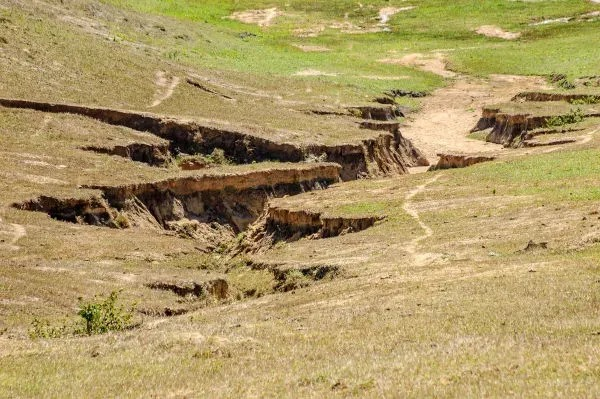
\includegraphics[width=\textwidth,height=4.4cm,keepaspectratio]{figures/foto_pastagem_ravinas.jpg}
    \par\small\textbf{(A)} Pastagem degradada com ravinas escalonadas e solo exposto.
  \end{minipage}\hfill
  \begin{minipage}[t]{0.48\textwidth}
    \centering
    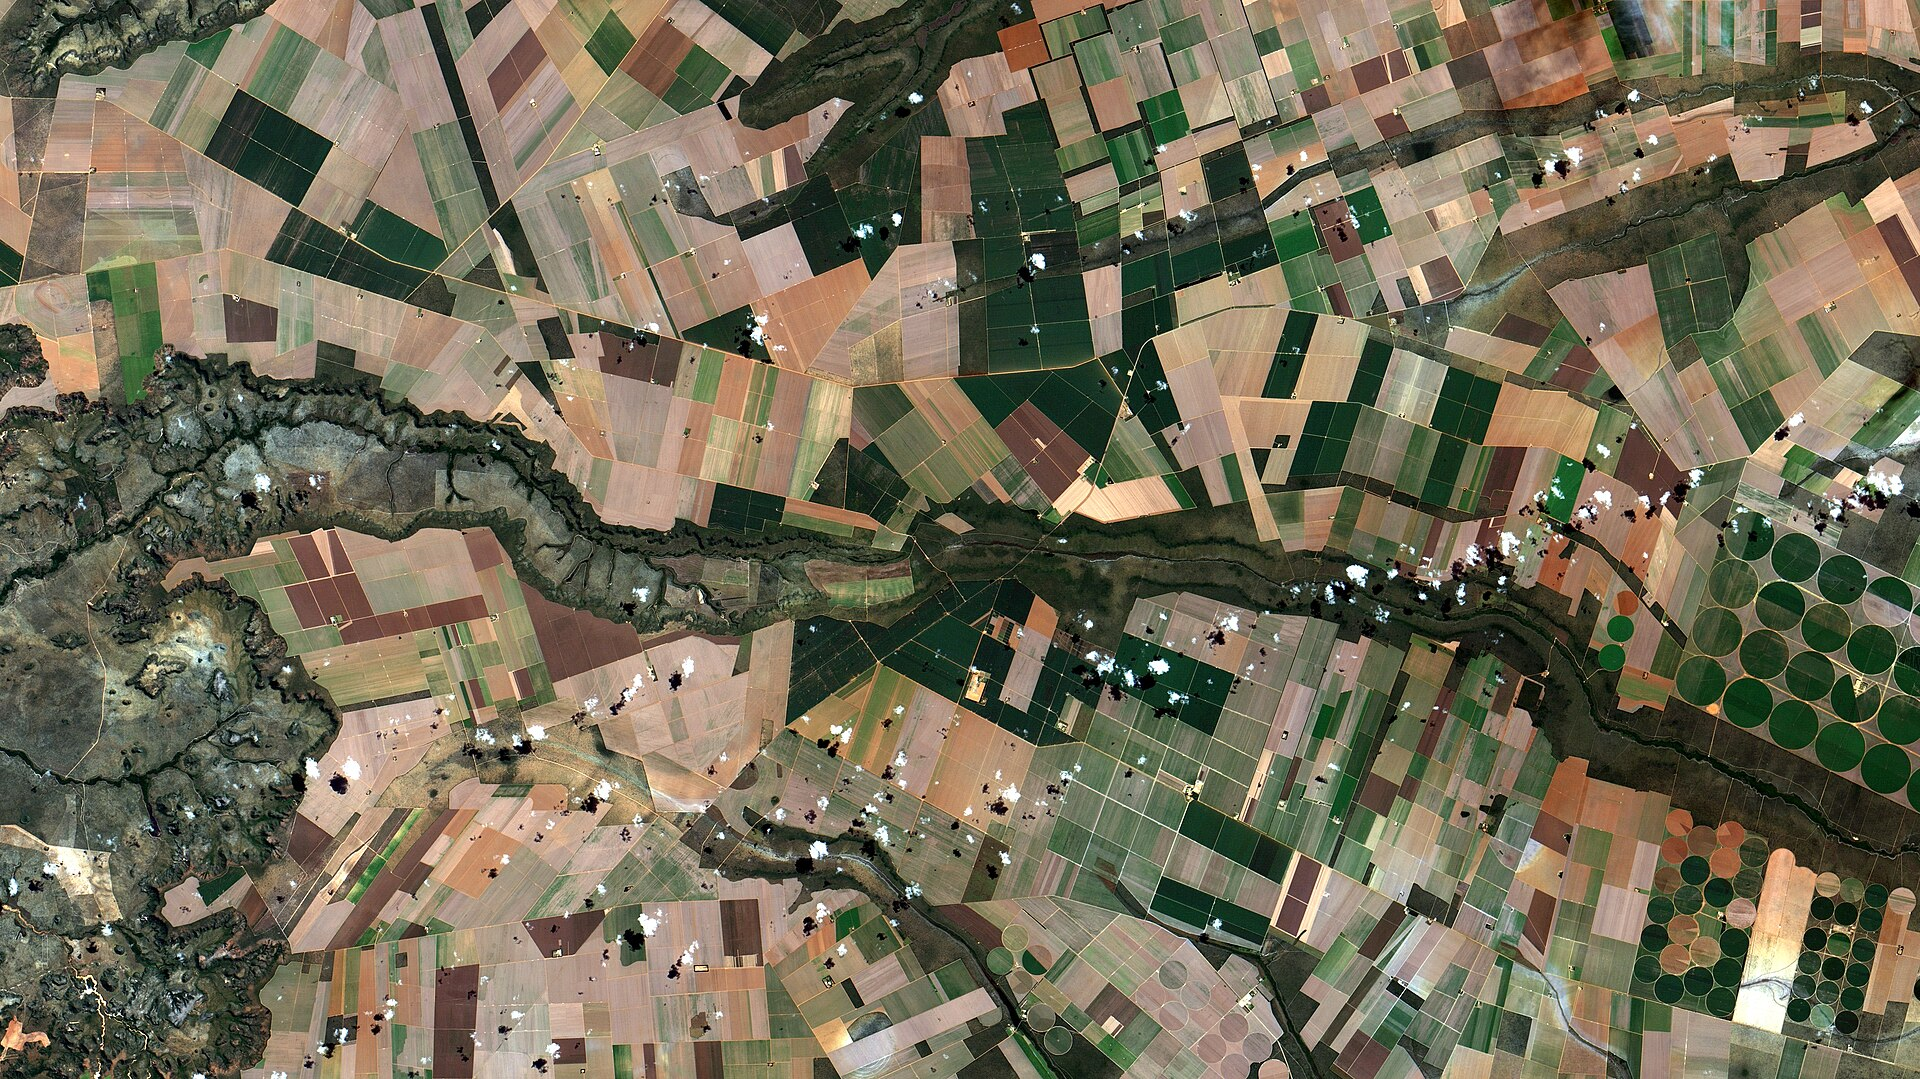
\includegraphics[width=\textwidth,height=4.4cm,keepaspectratio]{figures/foto_pivos_oeste_baiano.jpg}
    \par\small\textbf{(B)} Pivôs centrais de irrigação no Cerrado do Oeste Baiano (CBERS-4 MUX).
  \end{minipage}
  \caption{\textbf{Vetores de mudança no uso da terra na Bahia.} \textit{O que observar:} no painel A, a perda de cobertura vegetal em áreas de pastoreio intensivo expõe o solo ao escoamento concentrado e desencadeia incisões erosivas escalonadas. No painel B, os círculos escuros evidenciam a conversão em larga escala das chapadas do Oeste Baiano por agricultura irrigada mecanizada, elevando a pressão sobre a recarga hídrica. Fonte: Acervo didático CHF662 (A) e INPE/Wikimedia Commons, CC BY-SA (B).}
  \label{fig:vetores_bahia}
\end{figure}


\subsection{Degradação dos Solos e Processos Erosivos}

O solo não é um substrato inerte sobre o qual se constroem edificações ou se aplicam fertilizantes; trata-se de um corpo natural tridimensional, dinâmico e vivo, cuja formação (pedogênese) demanda séculos ou milênios. A degradação edáfica manifesta-se pela perda progressiva de suas funções físicas, químicas e biológicas: redução do teor de matéria orgânica, quebra dos agregados, selamento superficial, compactação pelo pisoteio animal ou tráfego de máquinas, salinização em perímetros irrigados mal drenados e remoção acelerada de partículas pela erosão hídrica e eólica.

Quando a taxa de remoção de solo supera amplamente a taxa natural de formação, a erosão evolui da forma \emph{laminar} (lavagem difusa da camada superficial mais fértil) para a forma \emph{linear} (sulcos, ravinas e voçorocas). Os sedimentos mobilizados das encostas não desaparecem: são transportados pela rede de drenagem e depositados em calhas fluviais, barreiros, cisternas rurais e açudes, reduzindo sua capacidade de armazenamento de água.

\subsection{Escassez Hídrica: Condição Climática versus Produção Socioambiental}

Um dos equívocos mais persistentes sobre o Nordeste brasileiro é explicar a escassez hídrica exclusivamente pela baixa média pluviométrica. O clima semiárido apresenta, de fato, chuvas concentradas no tempo, elevada variabilidade interanual e altas taxas de evapotranspiração potencial, características naturais que definem a \textbf{semiaridez}. Contudo, a \textbf{escassez hídrica vivenciada pela população} é resultado direto da interação entre essa dinâmica climática e fatores socioespaciais: desmatamento das cabeceiras e matas ciliares, compactação do solo (que impede a recarga do lençol freático), assoreamento de reservatórios, contaminação de mananciais e distribuição desigual da infraestrutura de captação e acesso à água.

\begin{boxConceito}[Cadeia de Retroalimentação Solo--Água--Uso da Terra]
  
Degradação dos solos, escassez hídrica e mudança no uso da terra não ocorrem como listas paralelas de problemas: elas formam um circuito retroalimentado. A supressão vegetal reduz a infiltração e intensifica o escoamento superficial; o escoamento acelerado remove o solo fértil e assoreia os corpos d'água; a perda de fertilidade e de disponibilidade hídrica pressiona os produtores a expandir o desmatamento sobre novas áreas frágeis, ampliando a vulnerabilidade socioambiental.
\end{boxConceito}

\begin{center}
\begin{tikzpicture}[
  node distance=0.45cm and 0.55cm,
  stepbox/.style={draw=uefsNavy, fill=bgSoft, rounded corners=3pt, line width=0.8pt, align=center, font=\footnotesize, inner sep=5pt, text width=3.2cm},
  alertbox/.style={draw=uefsAlert, fill=bgAlert, rounded corners=3pt, line width=0.9pt, align=center, font=\footnotesize, inner sep=5pt, text width=3.3cm},
  arr/.style={-{Stealth[length=2.2mm]}, line width=0.9pt, color=uefsNavy}
]
  \node[stepbox] (s1) at (0,0) {\textbf{1. Mudança no uso da terra}\\Supressão da Caatinga e sobrepastoreio};
  \node[stepbox] (s2) at (4.1,0) {\textbf{2. Degradação do solo}\\Exposição, selamento e menor infiltração};
  \node[stepbox] (s3) at (8.2,0) {\textbf{3. Dinâmica erosiva}\\Escoamento rápido, sulcos e ravinas};
  \node[alertbox] (s4) at (12.3,0) {\textbf{4. Escassez e risco}\\Assoreamento, menor recarga e vulnerabilidade};

  \draw[arr] (s1) -- (s2);
  \draw[arr] (s2) -- (s3);
  \draw[arr] (s3) -- (s4);

  % Seta de retroalimentação inferior
  \draw[arr, color=uefsAlert, dashed, line width=0.9pt] (s4.south) -- ++(0,-0.65) -| node[pos=0.25, below, font=\scriptsize\itshape, color=uefsAlert]{Retroalimentação positiva (ciclo amplificador): queda de produtividade pressiona novas áreas frágeis} (s1.south);
\end{tikzpicture}
\par\smallskip
{\small\color{uefsMuted}\textbf{Esquema 1.2:} Cadeia processual de retroalimentação entre uso da terra, degradação edáfica e escassez hídrica em ambientes semiáridos.}
\end{center}

\section{O Debate Crítico: Desenvolvimento Sustentável versus Sustentabilidade}

A partir da publicação do Relatório \emph{Nosso Futuro Comum} (Relatório Brundtland, 1987) e da Conferência das Nações Unidas sobre Meio Ambiente e Desenvolvimento (Rio-92), a expressão \textbf{desenvolvimento sustentável} ganhou enorme visibilidade internacional, sendo definida como aquele capaz de atender às necessidades do presente sem comprometer a capacidade das gerações futuras de atenderem às suas próprias necessidades.

À primeira vista, a formulação parece consensual e inquestionável. Entretanto, autores como Carlos Walter Porto-Gonçalves (\emph{Os (des)caminhos do meio ambiente}, 2006) e Enrique Leff (2001) demonstram que o conceito abriga contradições profundas. Porto-Gonçalves chama atenção para a estrutura política da expressão: ao acoplar o adjetivo ``sustentável'' ao substantivo ``desenvolvimento'', o discurso institucional dominante preserva intacto o projeto desenvolvimentista baseado na expansão contínua da produção de mercadorias, no consumo crescente de energia e na subordinação de territórios periféricos ao mercado mundial.

Sob essa perspectiva crítica, a noção de desenvolvimento sustentável muitas vezes opera como mecanismo de \emph{recodificação econômica da natureza}: a floresta, a água e o clima passam a ser valorados apenas como ``capital natural'' ou ``serviços mercantilizáveis'', sem questionar quem detém o controle dos territórios, quem se beneficia dos ganhos econômicos e quem arca com a poluição, o deslocamento compulsório e a degradação do solo.

Em contraposição, o debate sobre \textbf{sustentabilidade} (ou sustentabilidade socioambiental) propõe deslocar o foco do crescimento econômico ilimitado para a manutenção da integridade ecológica, da diversidade cultural e da equidade territorial. A sustentabilidade, nesse sentido, não é um selo de marketing empresarial nem uma meta técnica universalmente imposta de cima para baixo, mas um projeto histórico e geográfico que reconhece os limites biofísicos dos ecossistemas e valoriza modos locais de convivência com o ambiente, como as estratégias de convivência com o Semiárido baseadas em conservação de solo, captação descentralizada de água de chuva e manejo sustentável da Caatinga.

\begin{center}
\renewcommand{\arraystretch}{1.24}
\small
\begin{tabularx}{\textwidth}{@{}p{3.0cm} p{6.2cm} >{\raggedright\arraybackslash}X@{}}
  \toprule
  \rowcolor{uefsNavy}
  \textcolor{white}{\bfseries Critério de Análise} & \textcolor{white}{\bfseries Discurso Hegemônico de Desenvolvimento Sustentável} & \textcolor{white}{\bfseries Perspectiva Crítica de Sustentabilidade Socioambiental} \\
  \midrule
  \textbf{Eixo central} & Conciliar crescimento econômico contínuo com eficiência tecnológica e controle de impactos. & Garantir integridade dos sistemas ecológicos, justiça socioambiental e reprodução digna da vida. \\
  \rowcolor{bgGray}
  \textbf{Leitura da natureza} & Capital natural, estoque de recursos mensuráveis pelo mercado e ativos compensáveis. & Patrimônio socioecológico complexo, dotado de limites biofísicos e significados culturais plurais. \\
  \textbf{Papel da técnica} & Solução principal para a crise (ecoeficiência, substituição de insumos, mercado verde). & Ferramenta necessária, mas subordinada a critérios éticos, ecológicos e democráticos de decisão. \\
  \rowcolor{bgGray}
  \textbf{Relação com o território} & Tende a homogeneizar modelos produtivos e minimizar conflitos distributivos. & Reconhece conflitos territoriais, desigualdades de poder e diversidade de saberes locais. \\
  \textbf{Referência-base} & Crítica formulada em Leff (2001, cap. 2) e Porto-Gonçalves (2006). & Proposta articulada em Leff (2001), Porto-Gonçalves (2006) e na Geografia Socioambiental. \\
  \bottomrule
\end{tabularx}
\par\smallskip
{\small\color{uefsMuted}\textbf{Tabela 1.2:} Síntese comparativa entre o discurso convencional de desenvolvimento sustentável e a perspectiva crítica de sustentabilidade.}
\end{center}

\section{Planejamento Ambiental e o Papel Integrador da Geografia}

Diante de uma crise simultaneamente ecológica, econômica e territorial, o \textbf{planejamento ambiental} apresenta-se como instrumento fundamental de mediação entre a dinâmica da natureza e as demandas da sociedade. Planejar ambientalmente significa ir além de ações emergenciais pós-desastre: envolve levantar evidências empíricas sobre o meio físico, biótico e socioespacial (diagnóstico), projetar tendências de degradação ou recuperação sob diferentes cenários de uso da terra (prognóstico), estabelecer diretrizes de zoneamento, conservação e restauração (ordenamento) e acompanhar continuamente os resultados por meio de indicadores auditáveis (monitoramento).

É precisamente nesse terreno que a \textbf{Geografia} desempenha um papel integrador insubstituível frente à fragmentação disciplinar:
\begin{enumerate}[leftmargin=1.6em, itemsep=2.5pt]
  \item \textbf{Articulação físico-biótico--socioespacial:} a formação geográfica capacita o profissional a ler simultaneamente o relevo, os solos, a rede de drenagem e a cobertura vegetal juntamente com a estrutura fundiária, a urbanização, as redes de infraestrutura e os conflitos territoriais.
  \item \textbf{Domínio da espacialidade e da cartografia:} problemas ambientais nunca são abstratos; eles têm localização, extensão, conectividade e padrões espaciais que podem ser mapeados, modelados e cruzados em Sistemas de Informação Geográfica (SIG) e trabalhos de campo.
  \item \textbf{Leitura multiescalar:} o(a) geógrafo(a) conecta processos que ocorrem na escala da parcela de solo ou da vertente (erosão em sulcos) com a escala da bacia hidrográfica (assoreamento de mananciais), da região (políticas para o Semiárido) e das redes econômicas globais (demanda por energia e commodities).
  \item \textbf{Mediação interdisciplinar:} por transitar entre as ciências da Terra e as ciências humanas, a Geografia atua como ponte entre engenheiros, biólogos, agrônomos, gestores públicos e comunidades locais na construção de diagnósticos ambientais coerentes.
\end{enumerate}

\begin{boxDica}[Conexão Direta com os Próximos Módulos e o Trabalho Prático Final]
Tudo o que você estudará nos próximos capítulos de CHF662 desdobra os fundamentos apresentados aqui: no Módulo 2, a Avaliação de Impacto Ambiental (AIA) e a análise integrada; no Módulo 3, a bacia hidrográfica, a morfopedologia, os geossistemas e a fragilidade ambiental; no Módulo 4, os indicadores ambientais e de qualidade do solo (incluindo a viagem de campo no Semiárido Baiano); e no Módulo 5, a bioengenharia de água e solo, a legislação e o Diagnóstico Ambiental Aplicado (50\% da nota final). Manter desde o Capítulo 1 o hábito de integrar processos naturais e decisões sociais evitará diagnósticos fragmentados na Prova Teórica e no Trabalho Final.
\end{boxDica}

% ----------------------------------------------------------------------------
% ETAPA 4 — ESTUDOS DE CASO E EXEMPLOS RESOLVIDOS PASSO A PASSO
% ----------------------------------------------------------------------------
\etapa{4}{ESTUDOS DE CASO E EXEMPLOS RESOLVIDOS PASSO A PASSO}

\noindent\textit{Nota metodológica:} Os cenários numéricos e localidades estilizadas abaixo são \textbf{cenários didáticos ilustrativos}, construídos exclusivamente para treinar a aplicação rigorosa dos referenciais teóricos de Leff (2001) e Porto-Gonçalves (2006) a situações concretas da prática geográfica.

\begin{boxExemplo}{1.1: Básico}{Fragmentação Disciplinar em Projeto de Contenção de Erosão}
\passoEnunciado{Em um município fictício do Semiárido Baiano \textit{(cenário didático ilustrativo)}, uma prefeitura contratou uma empresa para conter o assoreamento de um açude comunitário. A equipe técnica elaborou apenas um projeto de dragagem mecânica do reservatório e construção de um muro de concreto próximo ao sangradouro, sem avaliar o uso do solo nas cabeceiras da microbacia nem ouvir os agricultores que utilizam a água. Dois anos após a obra, o açude voltou a apresentar acúmulo intenso de sedimentos.}
\passoDados{Intervenção exclusivamente estrutural/corretiva (dragagem e muro de concreto); ausência de diagnóstico da cobertura vegetal e dos solos nas vertentes a montante; ausência de participação dos usuários locais; retorno do assoreamento em 2 anos.}
\passoPedido{Diagnosticar a falha epistemológica e metodológica do projeto à luz de Enrique Leff (2001) e indicar como uma abordagem interdisciplinar geográfica reestruturaria a intervenção.}
\passoMetodo{Análise epistemológica baseada nos conceitos de \emph{racionalidade econômica/instrumental}, \emph{fragmentação disciplinar}, \emph{saber ambiental} e \emph{interdisciplinaridade} (Leff, 2001, cap. 2).}
\passoContas{%
  \begin{enumerate}[leftmargin=1.5em, itemsep=2pt]
    \item \textbf{Identificação do sintoma versus causa:} a dragagem atuou apenas sobre o sintoma final (sedimento acumulado no açude), ignorando a causa geradora nas vertentes a montante (solo exposto, erosão laminar e linear, retirada da vegetação ripária).
    \item \textbf{Diagnóstico epistemológico (Leff, 2001):} o projeto reproduziu a \emph{fragmentação disciplinar} e a \emph{racionalidade instrumental}, tratando um problema socioambiental complexo como mera questão pontual de engenharia civil.
    \item \textbf{Reestruturação interdisciplinar:} uma equipe coordenada sob perspectiva geográfica integrada deveria: (a) delimitar a microbacia de contribuição do açude; (b) mapear áreas de solo exposto, sobrepastoreio e focos erosivos nas cabeceiras; (c) dialogar com os agricultores para identificar pressões de uso da terra e saberes locais de manejo; e (d) combinar medidas conservacionistas na vertente (recomposição vegetal, retenção de enxurrada, manejo do pastoreio) com ações de manutenção do reservatório.
  \end{enumerate}
}
\passoResposta{O fracasso recorrente do projeto decorre da fragmentação disciplinar e da racionalidade instrumental, que trataram o assoreamento como falha pontual dissociada da dinâmica da microbacia e do uso social da terra. A solução exige abordagem interdisciplinar e planejamento integrado a montante e junto à comunidade.}
\passoVerificacao{A análise é ambientalmente coerente: dragar um açude sem reduzir a produção de sedimentos nas encostas apenas reinicia o ciclo de assoreamento a cada estação chuvosa, desperdiçando recursos públicos e mantendo a vulnerabilidade hídrica.}
\end{boxExemplo}

\begin{boxExemplo}{1.2: Básico}{Diferenciando Semiaridez Climática de Escassez Hídrica Socioambiental}
\passoEnunciado{Duas microbacias rurais vizinhas no Semiárido Baiano \textit{(cenário didático ilustrativo)} registram exatamente a mesma precipitação média anual de $580\text{ mm}$, concentrada entre novembro e março, sobre substrato geológico e relevo semelhantes. Na Microbacia A, $65\%$ da área mantém cobertura de Caatinga manejada, faixas de mata ciliar conservadas e práticas de retenção de água no solo; suas cacimbas permanecem com água na estação seca. Na Microbacia B, $78\%$ da área foi convertida em pastagem degradada com solo compactado e margens desmatadas; os reservatórios secam rapidamente após as chuvas e o solo apresenta sulcos erosivos.}
\passoDados{Precipitação idêntica ($580\text{ mm/ano}$) e substrato semelhante em ambas as microbacias. Microbacia A: $65\%$ de vegetação nativa, mata ciliar preservada, disponibilidade hídrica mantida na estiagem. Microbacia B: $78\%$ de pastagem degradada, solo compactado, margens desmatadas, rápida perda de água e erosão em sulcos.}
\passoPedido{Explicar por que o determinismo climático não explica a diferença observada entre as duas microbacias e demonstrar a relação causal entre uso da terra, solo e água.}
\passoMetodo{Análise comparativa controlada (mesmo clima, diferentes usos da terra) articulando processos hidrogeomorfológicos básicos e leitura socioambiental da escassez hídrica.}
\passoContas{%
  \begin{enumerate}[leftmargin=1.5em, itemsep=2pt]
    \item \textbf{Controle da variável climática:} como ambas as microbacias recebem $580\text{ mm/ano}$ sob o mesmo regime de chuvas concentradas, a diferença na disponibilidade de água na estação seca não pode ser atribuída apenas à falta de chuva.
    \item \textbf{Dinâmica na Microbacia A:} a cobertura vegetal protege a superfície do solo contra o impacto das gotas de chuva, mantém porosidade elevada e favorece a infiltração, recarregando o solo e os reservatórios rasos (cacimbas) para o período seco.
    \item \textbf{Dinâmica na Microbacia B:} a remoção da vegetação e a compactação reduzem a taxa de infiltração; assim, grande parcela dos $580\text{ mm}$ transforma-se rapidamente em escoamento superficial, gerando sulcos erosivos, arraste de sedimentos e baixa recarga hídrica subsuperficial.
    \item \textbf{Síntese conceitual:} a semiaridez é condição climática natural comum às duas áreas, mas a escassez hídrica severa na Microbacia B é agravada pelo modelo de uso e ocupação do solo.
  \end{enumerate}
}
\passoResposta{A diferença decorre do manejo do uso da terra e das condições do solo, e não apenas do clima: a degradação vegetal e edáfica na Microbacia B converte a chuva em escoamento rápido e erosão, reduzindo a infiltração e produzindo escassez hídrica socioambiental.}
\passoVerificacao{O raciocínio respeita o balanço hídrico elementar: para uma mesma entrada pluviométrica ($P = 580\text{ mm}$), quanto menor a infiltração em solos degradados, maior o escoamento superficial imediato e menor a água armazenada disponível durante a estiagem.}
\end{boxExemplo}

\begin{figure}[H]
  \centering
  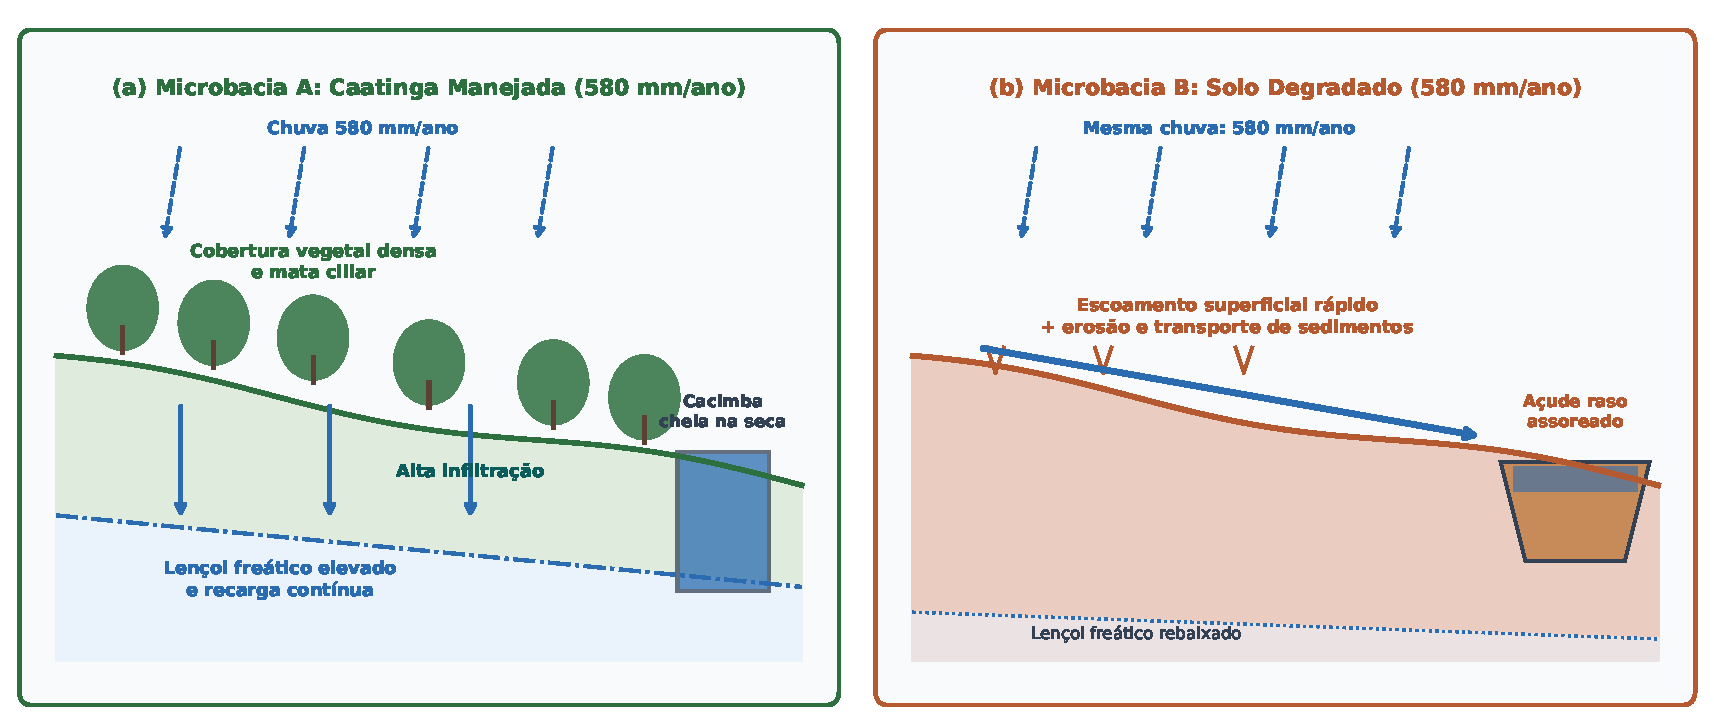
\includegraphics[width=0.96\textwidth]{figures/fig_cap01_contraste_microbacias.pdf}
  \caption{\textbf{Contraste hidrogeomorfológico entre semiaridez climática e escassez socioambiental.} \textit{O que observar:} sob a mesma precipitação anual de 580 mm, a Microbacia A conserva a cobertura arbustiva, favorece a infiltração e mantém o lençol freático elevado para abastecimento em cacimbas. Na Microbacia B, a compactação do solo redireciona a água para o escoamento superficial rápido, acelerando a erosão e o assoreamento do açude. Fonte: Elaboração didática CHF662.}
  \label{fig:contraste_microbacias}
\end{figure}


\begin{boxExemplo}{1.3: Intermediário}{Análise Crítica de um Discurso de ``Desenvolvimento Sustentável''}
\passoEnunciado{Um consórcio agroindustrial divulga um documento promocional anunciando a implantação de um polo de monocultura irrigada de exportação em uma bacia hidrográfica de transição Cerrado--Caatinga \textit{(cenário didático ilustrativo)}. O texto classifica o empreendimento como exemplo de ``desenvolvimento sustentável'' porque utilizará pivôs com sensores digitais que economizam $15\%$ de água em comparação a sistemas antigos e compensará a supressão de vegetação nativa mediante a compra de créditos ambientais em outra região do país.}
\passoDados{Alegações do consórcio: ganho de $15\%$ na eficiência de irrigação por sensores; compensação ambiental fora da bacia impactada; expansão de monocultura intensiva com remoção de vegetação nativa local e aumento da captação hídrica total.}
\passoPedido{Avaliar criticamente o uso do termo ``desenvolvimento sustentável'' nesse documento à luz de Porto-Gonçalves (2006) e Leff (2001), apontando as limitações socioambientais ocultadas pela peça promocional.}
\passoMetodo{Análise crítica do discurso ambiental com base na distinção entre \emph{desenvolvimento sustentável hegemônico} e \emph{sustentabilidade socioambiental} (Porto-Gonçalves, 2006; Leff, 2001).}
\passoContas{%
  \begin{enumerate}[leftmargin=1.5em, itemsep=2pt]
    \item \textbf{Análise do ganho de ecoeficiência ($15\%$):} economizar água por hectare em relação a técnicas antigas não garante redução do consumo total de água na bacia se a área irrigada se expandir de forma absoluta. A técnica melhora a eficiência produtiva sem questionar o limite hídrico regional.
    \item \textbf{Crítica à compensação desterritorializada:} comprar créditos ambientais em outra região trata a natureza como mercadoria intercambiável (lógica da racionalidade econômica criticada por Leff, 2001). Contudo, a biodiversidade, a proteção do solo e a recarga hídrica perdidas na bacia local não são fisicamente repostas por uma área conservada a centenas de quilômetros.
    \item \textbf{Ocultamento de dimensões sociais (Porto-Gonçalves, 2006):} o discurso adota o adjetivo ``sustentável'' para legitimar o modelo desenvolvimentista, omitindo questões centrais como quem perde acesso à água a jusante, como se alteram a estrutura fundiária e a segurança alimentar local e se as comunidades atingidas participaram da decisão.
  \end{enumerate}
}
\passoResposta{O documento emprega ``desenvolvimento sustentável'' em sentido retórico e mercadológico: reduz a questão ambiental à eficiência tecnológica parcial e à compensação financeira fora do território, desconsiderando limites hídricos da bacia e impactos socioespaciais locais.}
\passoVerificacao{A crítica é equilibrada e rigorosa: não nega a utilidade de sensores de irrigação, mas demonstra que eficiência técnica isolada não equivale à sustentabilidade ecológica e social em escala de bacia hidrográfica.}
\end{boxExemplo}

\begin{boxExemplo}{1.4: Intermediário}{Quantificação Didática de Mudanças no Uso da Terra em Microbacia}
\passoEnunciado{Durante um exercício de diagnóstico preliminar sobre uma microbacia fictícia de $1.200\text{ ha}$ no Semiárido Baiano \textit{(cenário didático ilustrativo)}, uma turma de Geografia comparou o mapeamento de uso e cobertura da terra entre dois anos de referência ($t_0$ e $t_1$, com intervalo de 15 anos) e obteve a tabela abaixo:}
\passoDados{%
  Área total da microbacia: $A_{\text{total}} = 1.200\text{ ha}$. Distribuição por classe:
  \begin{itemize}[leftmargin=1.5em, itemsep=1pt]
    \item Caatinga arbóreo-arbustiva densa: $660\text{ ha}$ em $t_0$ e $360\text{ ha}$ em $t_1$;
    \item Pastagem manejada e agricultura familiar diversificada: $300\text{ ha}$ em $t_0$ e $270\text{ ha}$ em $t_1$;
    \item Pastagem degradada com cobertura rala: $180\text{ ha}$ em $t_0$ e $390\text{ ha}$ em $t_1$;
    \item Solo exposto / áreas com erosão visível: $60\text{ ha}$ em $t_0$ e $180\text{ ha}$ em $t_1$.
  \end{itemize}
}
\passoPedido{(a) Calcular a variação absoluta (em $\text{ha}$), a variação relativa percentual de cada classe e a participação percentual das classes degradadas (pastagem degradada + solo exposto) em $t_0$ e $t_1$; (b) interpretar geograficamente o significado ambiental dessa trajetória.}
\passoMetodo{Cálculo passo a passo de variações absolutas ($\Delta A = A_{t_1} - A_{t_0}$), relativas ($\Delta\% = \frac{A_{t_1} - A_{t_0}}{A_{t_0}} \times 100\%$) e proporções sobre a área total ($p = \frac{A}{A_{\text{total}}} \times 100\%$), seguido de interpretação integrada solo--água--uso da terra.}
\passoContas{%
  \begin{enumerate}[leftmargin=1.5em, itemsep=2.5pt]
    \item \textbf{Conferência da área total:}
    Em $t_0$: $660 + 300 + 180 + 60 = 1.200\text{ ha}$.
    Em $t_1$: $360 + 270 + 390 + 180 = 1.200\text{ ha}$. (Conservação da área verificada.)

    \item \textbf{Variação absoluta ($\Delta A$) e relativa ($\Delta\%$) por classe:}
    \begin{itemize}[leftmargin=1.4em, itemsep=1.5pt]
      \item \emph{Caatinga densa:} $\Delta A = 360 - 660 = -300\text{ ha}$; $\Delta\% = \frac{-300}{660} \times 100\% \approx -45,5\%$.
      \item \emph{Pastagem manejada / agricultura familiar:} $\Delta A = 270 - 300 = -30\text{ ha}$; $\Delta\% = \frac{-30}{300} \times 100\% = -10,0\%$.
      \item \emph{Pastagem degradada:} $\Delta A = 390 - 180 = +210\text{ ha}$; $\Delta\% = \frac{+210}{180} \times 100\% \approx +116,7\%$.
      \item \emph{Solo exposto / erosão visível:} $\Delta A = 180 - 60 = +120\text{ ha}$; $\Delta\% = \frac{+120}{60} \times 100\% = +200,0\%$.
    \end{itemize}

    \item \textbf{Participação conjunta das classes degradadas sobre a área total:}
    \begin{itemize}[leftmargin=1.4em, itemsep=1.5pt]
      \item Em $t_0$: $A_{\text{deg},0} = 180 + 60 = 240\text{ ha} \implies p_0 = \frac{240}{1.200} \times 100\% = 20,0\%$.
      \item Em $t_1$: $A_{\text{deg},1} = 390 + 180 = 570\text{ ha} \implies p_1 = \frac{570}{1.200} \times 100\% = 47,5\%$.
      \item Acréscimo na participação degradada: $47,5\% - 20,0\% = +27,5\text{ pontos percentuais}$ (ou $+330\text{ ha}$).
    \end{itemize}

    \item \textbf{Interpretação geográfica integrada:} em 15 anos, a microbacia perdeu $45,5\%$ de sua cobertura nativa densa, enquanto a área de solo exposto triplicou ($+200\%$). Em $t_1$, quase metade da microbacia ($47,5\%$) encontra-se sob cobertura rala ou sem proteção vegetal, indicando elevada exposição à erosão hídrica, provável redução da infiltração, aceleração do escoamento superficial e risco crescente de assoreamento dos corpos d'água e queda de renda rural.
  \end{enumerate}
}
\passoResposta{A Caatinga densa retraiu $-300\text{ ha}$ ($-45,5\%$), o solo exposto triplicou ($+120\text{ ha}$; $+200,0\%$) e as classes degradadas saltaram de $20,0\%$ para $47,5\%$ da microbacia, configurando um quadro crítico de degradação hidrogeomorfológica e perda de sustentabilidade territorial.}
\passoVerificacao{Verificação aritmética e física: a soma das variações absolutas anula-se ($-300 - 30 + 210 + 120 = 0\text{ ha}$), confirmando consistência matemática; ambientalmente, o avanço de $27,5$ pontos percentuais de áreas degradadas justifica prioridade imediata de planejamento conservacionista e recuperação.}
\end{boxExemplo}

\begin{boxExemplo}{1.5: Avançado}{Diretrizes de Planejamento Ambiental Integrado em Área de Múltiplas Pressões}
\passoEnunciado{Na periferia de uma cidade média do interior da Bahia \textit{(cenário didático ilustrativo)}, uma bacia hidrográfica de pequeno porte concentra quatro processos simultâneos: (i) expansão de loteamentos populares sem drenagem pluvial em encostas de declividade moderada a forte; (ii) supressão da vegetação ciliar de um riacho intermitente que abastece hortas periurbanas; (iii) extração irregular de areia no leito do riacho para a construção civil; e (iv) lançamento de esgoto doméstico sem tratamento. A administração municipal propôs apenas ``multar os pequenos agricultores'' e ``canalizar o riacho com concreto''.}
\passoDados{Quatro vetores simultâneos de pressão (urbanização sem drenagem, desmatamento ciliar, mineração irregular de areia e esgoto doméstico) atuando na mesma microbacia; proposta municipal restrita a punição seletiva e canalização rígida.}
\passoPedido{Criticar a proposta municipal usando os conceitos de crise de racionalidade (Leff, 2001) e sustentabilidade crítica (Porto-Gonçalves, 2006) e formular quatro diretrizes integradas de planejamento ambiental lideradas por uma perspectiva geográfica.}
\passoMetodo{Integração dos referenciais epistemológicos do capítulo (Leff, 2001; Porto-Gonçalves, 2006) com os princípios do planejamento ambiental geográfico (diagnóstico multiescalar, interdisciplinaridade e participação social).}
\passoContas{%
  \begin{enumerate}[leftmargin=1.5em, itemsep=2.5pt]
    \item \textbf{Crítica à proposta municipal:}
    \begin{itemize}[leftmargin=1.4em, itemsep=1.5pt]
      \item \emph{Racionalidade instrumental:} canalizar o riacho com concreto transfere a velocidade do escoamento para jusante, agrava enchentes em outros trechos e elimina a função ecológica da calha natural, sem resolver o lançamento de esgoto nem a erosão das encostas.
      \item \emph{Injustiça socioambiental:} responsabilizar apenas os pequenos agricultores ignora a ausência de políticas habitacionais e de saneamento básico, bem como a cadeia econômica da construção civil que demanda areia ilegal.
    \end{itemize}
    \item \textbf{Quatro diretrizes integradas de planejamento ambiental:}
    \begin{itemize}[leftmargin=1.4em, itemsep=1.5pt]
      \item \emph{Diretriz 1, Diagnóstico espacial integrado da microbacia:} mapear uso da terra, áreas de risco nas encostas, pontos de lançamento de efluentes, cavas de extração mineral e trechos de APP degradada.
      \item \emph{Diretriz 2, Ordenamento territorial e saneamento:} disciplinar a expansão urbana, implantar drenagem sustentável (pavimentos permeáveis e bacias de retenção) e universalizar a coleta e o tratamento de esgoto.
      \item \emph{Diretriz 3, Recuperação hidrogeomorfológica e controle da extração:} coibir a lavra ilegal de areia com fiscalização e alternativas regulamentadas, recompor a mata ciliar e adotar técnicas conservacionistas nas vertentes.
      \item \emph{Diretriz 4, Gestão participativa e apoio à agricultura periurbana:} instituir comitê ou fórum da microbacia envolvendo moradores, horticultores, técnicos e poder público, convertendo os agricultores em agentes de conservação em vez de bodes expiatórios.
    \end{itemize}
  \end{enumerate}
}
\passoResposta{A proposta municipal fracassa por adotar solução tecnocrática e socialmente injusta; o planejamento ambiental geográfico exige diagnosticar os quatro vetores na escala da microbacia e articular ordenamento urbano, saneamento, recuperação ripária e gestão participativa.}
\passoVerificacao{As quatro diretrizes atacam simultaneamente os processos físicos (escoamento, erosão, qualidade da água) e as causas socioespaciais (habitação precária, déficit de saneamento, cadeia da construção civil), refletindo a passagem da fragmentação para a racionalidade ambiental.}
\end{boxExemplo}

% ----------------------------------------------------------------------------
% ETAPA 5 — ERROS CONCEITUAIS E METODOLÓGICOS MAIS COMUNS
% ----------------------------------------------------------------------------
\etapa{5}{ERROS CONCEITUAIS E METODOLÓGICOS MAIS COMUNS}

\begin{boxErro}[Erro 1.1: Reduzir a Crise Ambiental à ``Falta de Consciência Individual'']
\textbf{Equívoco frequente:} atribuir a degradação dos solos, a poluição hídrica ou o desmatamento exclusivamente à ``falta de educação'' ou a maus hábitos individuais dos cidadãos.

\textbf{Por que está incorreto:} embora práticas educativas sejam relevantes, esse argumento oculta determinantes estruturais (modelo econômico, padrão de uso da terra, concentração fundiária, déficit de saneamento e decisões políticas) que Leff (2001) identifica como núcleo da crise civilizatória.

\textbf{Como evitar:} analise sempre a articulação entre comportamentos locais, estruturas produtivas, políticas públicas e interesses econômicos em disputa no território.
\end{boxErro}

\begin{boxErro}[Erro 1.2: Confundir Multidisciplinaridade com Interdisciplinaridade Ambiental]
\textbf{Equívoco frequente:} acreditar que um estudo ambiental torna-se interdisciplinar apenas por conter capítulos separados escritos por um geólogo, um biólogo e um sociólogo.

\textbf{Por que está incorreto:} a mera justaposição de textos especializados sem diálogo metodológico caracteriza \emph{multidisciplinaridade}. Como mostra Leff (2001), a \emph{interdisciplinaridade ambiental} exige construir problemas integrados e explicar como processos físicos, bióticos e sociais condicionam-se mutuamente.

\textbf{Como evitar:} em seus relatórios e provas, explicite sempre as \emph{conexões causais} entre as variáveis (por exemplo, como uma decisão econômica de uso da terra altera a infiltração e agrava o assoreamento).
\end{boxErro}

\begin{boxErro}[Erro 1.3: Usar ``Desenvolvimento Sustentável'' como Sinônimo Neutro de ``Sustentabilidade'']
\textbf{Equívoco frequente:} empregar ambos os termos indistintamente, assumindo que qualquer projeto rotulado como ``desenvolvimento sustentável'' é ecologicamente íntegro e socialmente justo.

\textbf{Por que está incorreto:} conforme demonstra Porto-Gonçalves (2006), ``desenvolvimento sustentável'' é um conceito em disputa que frequentemente subordina a conservação ambiental à lógica do crescimento econômico contínuo e à mercantilização da natureza.

\textbf{Como evitar:} ao analisar políticas ou projetos, pergunte sempre: \emph{sustentável para quem, em qual escala espacial e com quais custos ecológicos e territoriais?}
\end{boxErro}

\begin{boxErro}[Erro 1.4: Explicar a Degradação do Semiárido pelo Determinismo Climático]
\textbf{Equívoco frequente:} afirmar que a erosão dos solos e a escassez hídrica no Semiárido Baiano são ``consequências inevitáveis da falta de chuva''.

\textbf{Por que está incorreto:} a semiaridez é uma condição climática natural à qual a Caatinga é evolutivamente adaptada. A degradação severa do solo e a vulnerabilidade hídrica resultam da combinação entre chuvas concentradas e práticas inadequadas de desmatamento, sobrepastoreio, compactação e desigualdade no acesso à água.

\textbf{Como evitar:} separe claramente o que é \emph{condicionante climático natural} do que é \emph{processo agravado pelo manejo e pela organização socioespacial}.
\end{boxErro}

% ----------------------------------------------------------------------------
% ETAPA 6 — EXERCÍCIOS DE FIXAÇÃO
% ----------------------------------------------------------------------------
\etapa{6}{EXERCÍCIOS DE FIXAÇÃO}

\subsection*{Nível 1: Básicos (Compreensão Conceitual)}

\begin{enumerate}[leftmargin=1.8em, itemsep=4pt]
  \item Explique, com base em Enrique Leff (2001), por que a crise ambiental contemporânea não pode ser compreendida apenas como uma crise ecológica ou tecnológica, mas como uma crise civilizatória e de racionalidade.
  \espacoResolucao[1.8cm]

  \item Diferencie \emph{racionalidade econômica} de \emph{racionalidade ambiental} segundo Leff (2001), indicando o papel das chamadas ``externalidades'' no primeiro caso.
  \espacoResolucao[1.8cm]

  \item Apresente duas diferenças fundamentais entre a abordagem \emph{multidisciplinar} e a abordagem \emph{interdisciplinar} na elaboração de diagnósticos ambientais.
  \espacoResolucao[1.8cm]

  \item Explique por que a supressão da vegetação nativa desencadeia simultaneamente processos de degradação do solo e alterações na disponibilidade hídrica de uma microbacia.
  \espacoResolucao[1.8cm]

  \item Sintetize a diferença entre \emph{semiaridez climática} e \emph{escassez hídrica socioambiental} no contexto do Semiárido Baiano.
  \espacoResolucao[1.8cm]

\subsection*{Nível 2: Intermediários (Análise Crítica e Aplicação)}

  \item Com base em Porto-Gonçalves (2006), analise criticamente a tensão existente entre o substantivo ``desenvolvimento'' e o adjetivo ``sustentável'' na expressão \emph{desenvolvimento sustentável}.
  \espacoResolucao[1.8cm]

  \item Um município baiano pretende elaborar um plano de conservação de nascentes, mas contratou estudos isolados de geologia, botânica e economia que não se comunicam entre si. Identifique o limite metodológico desse procedimento e proponha como a Geografia pode exercer papel integrador nesse planejamento ambiental.
  \espacoResolucao[1.8cm]

  \item Em um cenário didático ilustrativo, uma microbacia de $800\text{ ha}$ no Semiárido passou, em 10 anos, de $520\text{ ha}$ para $320\text{ ha}$ de cobertura nativa de Caatinga, enquanto a área de solo exposto cresceu de $40\text{ ha}$ para $140\text{ ha}$. Calcule a variação absoluta (em $\text{ha}$) e percentual de ambas as classes e explique dois desdobramentos esperados sobre o escoamento superficial e o assoreamento local.
  \espacoResolucao[1.8cm]

  \item Compare brevemente os principais vetores contemporâneos de mudança no uso da terra no Semiárido Baiano e no Oeste Baiano (Cerrado), destacando como a escala regional orienta o diagnóstico geográfico.
  \espacoResolucao[1.8cm]

  \item Por que a adoção exclusiva de soluções de ecoeficiência (como redução pontual de consumo de insumos por unidade produzida) pode ser insuficiente para alcançar a sustentabilidade socioambiental de um território? Relacione sua resposta a Leff (2001).
  \espacoResolucao[1.8cm]

\subsection*{Nível 3: Aplicados e Objetivos (Múltipla Escolha)}

  \item Segundo Enrique Leff (2001, cap. 2), a construção do \emph{saber ambiental} frente à crise contemporânea implica:
  \begin{alternativas}
    \item Substituir integralmente as ciências naturais por análises filosóficas, dispensando medições empíricas de solo e água.
    \item Somar relatórios independentes de diferentes áreas técnicas sem alterar os pressupostos de cada disciplina.
    \item Questionar a fragmentação do conhecimento e a racionalidade econômica hegemônica, rearticulando saberes disciplinares e locais sob uma racionalidade ambiental.
    \item Transferir a resolução dos impactos ambientais exclusivamente aos mecanismos automáticos de precificação do mercado financeiro.
    \item Restringir o debate ambiental à preservação de parques isolados, desvinculando-o do planejamento territorial e produtivo.
  \end{alternativas}
  \espacoResolucao[1.8cm]

  \item A respeito da cadeia de processos que conecta mudanças no uso da terra, degradação dos solos e escassez hídrica no Semiárido Baiano, assinale a alternativa \textbf{correta}:
  \begin{alternativas}
    \item A baixa infiltração de água no solo depende apenas da quantidade anual de chuvas, não sofrendo influência da cobertura vegetal ou da compactação.
    \item A retirada da vegetação nativa e o sobrepastoreio ampliam a exposição do solo, reduzem a infiltração, aceleram o escoamento superficial e intensificam a erosão e o assoreamento de reservatórios.
    \item A erosão laminar restringe-se a regiões tropicais úmidas de Mata Atlântica, não ocorrendo em áreas de Caatinga devido à baixa precipitação anual.
    \item O assoreamento de açudes é um processo benéfico no Semiárido porque aumenta a profundidade útil dos reservatórios na estação seca.
    \item A escassez hídrica nordestina decorre unicamente de anomalias climáticas naturais, sem relação com o desmatamento ciliar ou a gestão territorial.
  \end{alternativas}
  \espacoResolucao[1.8cm]

  \item Na leitura crítica proposta por Porto-Gonçalves (2006) sobre o conceito de \emph{desenvolvimento sustentável}, destaca-se que:
  \begin{alternativas}
    \item A expressão representa um consenso científico definitivo e neutro, aceito sem tensões políticas por todos os grupos sociais.
    \item O conceito rompe integralmente com a lógica de expansão contínua da produção de mercadorias adotada desde a Revolução Industrial.
    \item O adjetivo ``sustentável'' muitas vezes funciona como verniz legitimador do modelo desenvolvimentista hegemônico, ocultando desigualdades territoriais e limites ecológicos.
    \item A sustentabilidade só pode ser atingida mediante a homogeneização cultural e a substituição de saberes locais por pacotes tecnológicos globais.
    \item O debate sobre sustentabilidade restringe-se à gestão de resíduos sólidos urbanos, não abrangendo conflitos agrários ou hídricos.
  \end{alternativas}
  \espacoResolucao[1.8cm]

  \item Qual atributo caracteriza mais adequadamente o papel integrador da Geografia no planejamento ambiental frente à fragmentação disciplinar?
  \begin{alternativas}
    \item A capacidade de articular componentes físico-bióticos e processos socioespaciais em múltiplas escalas, empregando leitura espacial, trabalho de campo e mediação interdisciplinar.
    \item A exclusividade na realização de análises laboratoriais químicas de água e solo, dispensando a colaboração com outras áreas científicas.
    \item O foco exclusivo na descrição de aspectos fisiográficos naturais, deixando os fatores econômicos e políticos fora do diagnóstico ambiental.
    \item A padronização de soluções técnicas idênticas para qualquer região do país, independentemente das especificidades locais de relevo, clima e cultura.
    \item A substituição do diagnóstico empírico prévio por intervenções emergenciais de engenharia após a ocorrência de desastres ambientais.
  \end{alternativas}
  \espacoResolucao[1.8cm]

  \item Considere um cenário didático ilustrativo em que uma área rural teve $300\text{ ha}$ de vegetação nativa suprimidos em uma microbacia de $1.000\text{ ha}$ que originalmente possuía $600\text{ ha}$ de vegetação nativa. Sobre essa mudança no uso da terra, é \textbf{correto} afirmar que:
  \begin{alternativas}
    \item A vegetação nativa sofreu redução relativa de $30\%$ em relação à sua área inicial.
    \item A participação da vegetação nativa na microbacia passou de $60\%$ para $30\%$, representando perda relativa de $50\%$ da cobertura nativa original.
    \item A participação da vegetação nativa passou de $50\%$ para $20\%$ da área total da microbacia.
    \item A mudança no uso da terra não produz efeitos hidrológicos relevantes enquanto restar pelo menos $20\%$ de cobertura vegetal.
    \item A redução relativa da vegetação nativa foi de $60\%$, correspondendo à mesma taxa de aumento do volume de água armazenado no solo.
  \end{alternativas}
  \espacoResolucao[1.8cm]
\end{enumerate}

% ----------------------------------------------------------------------------
% ETAPA 7 — QUESTÕES DE PROVAS, ENADE E CONCURSOS AMBIENTAIS
% ----------------------------------------------------------------------------
\etapa{7}{QUESTÕES DE PROVAS, ENADE E CONCURSOS AMBIENTAIS}

\begin{enumerate}[leftmargin=1.8em, itemsep=5pt, start=16]
  \item \textbf{(Questão autoral, estilo ENADE / Concurso Ambiental)} Um relatório técnico estadual diagnosticou a degradação de uma bacia hidrográfica semiárida em três capítulos redigidos sem integração: o primeiro descreveu litologia e solos; o segundo listou espécies da flora; e o terceiro apresentou indicadores de renda municipal. Ao final, o documento atribuiu a escassez hídrica ``exclusivamente ao baixo índice pluviométrico da região'' e sugeriu a construção de barragens de concreto como única medida necessária. Com base nos fundamentos da Análise Ambiental (Leff, 2001; Porto-Gonçalves, 2006), avalie as afirmações a seguir:
  \begin{enumerate}[label=\Roman*., leftmargin=1.6em, itemsep=1.5pt]
    \item O relatório exemplifica uma abordagem multidisciplinar fragmentada, e não uma análise interdisciplinar integrada.
    \item A conclusão do relatório incorre em determinismo climático ao ignorar o papel do uso da terra, da cobertura vegetal e da desigualdade de acesso à água na produção da escassez hídrica.
    \item A recomendação exclusiva de obras de concreto expressa uma racionalidade instrumental que desconsidera a dinâmica das vertentes e os saberes locais de convivência com o Semiárido.
    \item A separação estanque entre capítulos físicos e socioeconômicos é o procedimento ideal na Geografia por garantir neutralidade científica.
  \end{enumerate}
  É correto apenas o que se afirma em:
  \begin{alternativas}
    \item I e IV.
    \item II e IV.
    \item I, II e III.
    \item II, III e IV.
    \item I, II, III e IV.
  \end{alternativas}
  \espacoResolucao[1.8cm]

  \item \textbf{(Questão autoral, estilo ENADE / Concurso Ambiental)} Para o cargo de Analista Ambiental em órgão público de gestão territorial, exige-se domínio conceitual das diferenças entre crescimento econômico, desenvolvimento sustentável e sustentabilidade socioambiental. Considerando a abordagem crítica trabalhada na Geografia contemporânea (Leff, 2001; Porto-Gonçalves, 2006), assinale a alternativa que expressa corretamente uma diretriz coerente com a \textbf{racionalidade ambiental}:
  \begin{alternativas}
    \item Aceitar a degradação severa de cabeceiras de drenagem em regiões semiáridas desde que compensada pela compra de títulos financeiros ambientais em outros biomas.
    \item Subordinar o zoneamento ambiental de uma bacia hidrográfica exclusivamente à taxa de retorno econômico de curto prazo dos empreendimentos licenciados.
    \item Priorizar o planejamento ambiental integrado em escala de bacia, articulando conservação do solo e da água, limites biofísicos dos ecossistemas, equidade social e participação das populações locais.
    \item Transferir a responsabilidade integral pela recuperação de áreas degradadas a campanhas pontuais de sensibilização individual, dispensando instrumentos de ordenamento territorial.
    \item Adotar pacotes tecnológicos uniformes em todos os biomas brasileiros, desconsiderando a diversidade ecológica da Caatinga, do Cerrado e da Mata Atlântica.
  \end{alternativas}
  \espacoResolucao[1.8cm]

  \item \textbf{(Questão autoral, estilo ENADE / Concurso Ambiental)} Ao planejar o diagnóstico ambiental de uma microbacia sujeita à conversão acelerada de vegetação nativa em pastagens extensivas, um(a) geógrafo(a) propõe relacionar o mapeamento multitemporal de uso da terra com o levantamento de focos erosivos, a situação das matas ciliares e as condições socioeconômicas dos produtores rurais. Essa proposta metodológica reflete:
  \begin{alternativas}
    \item Uma postura estritamente naturalista, pois privilegia processos geomorfológicos em detrimento da organização espacial humana.
    \item O papel integrador da Geografia na Análise Ambiental, ao articular variáveis físico-bióticas e socioespaciais para identificar causas sistêmicas da degradação e subsidiar o planejamento territorial.
    \item Um procedimento disciplinar isolado, uma vez que o uso de mapas multitemporais dispensa o diálogo com outras ciências ambientais.
    \item A aplicação direta da racionalidade econômica clássica, pois trata a perda de solo apenas como custo externo sem repercussão territorial.
    \item Uma limitação de escala, pois a análise de microbacias impede compreender conexões com dinâmicas regionais ou políticas públicas de conservação.
  \end{alternativas}
  \espacoResolucao[1.8cm]
\end{enumerate}

\begin{boxDica}[Orientações para o Estudo Orientado e a Prova Dissertativa (Semana 10)]
A Avaliação Teórica de CHF662 (Semana 10) tem caráter predominantemente dissertativo. Para responder com excelência às questões sobre o Capítulo 1, estruture seus textos em três passos:
\begin{enumerate}[leftmargin=1.5em, itemsep=2pt]
  \item \textbf{Ancoragem conceitual explícita:} cite e defina com precisão os autores e categorias da ementa, como \emph{crise civilizatória}, \emph{racionalidade ambiental} e \emph{interdisciplinaridade} em Leff (2001); crítica ao \emph{desenvolvimento sustentável} em Porto-Gonçalves (2006).
  \item \textbf{Cadeia causal físico-social:} demonstre como mudanças no uso da terra acionam degradação do solo e escassez hídrica, evitando respostas vagas ou deterministas.
  \item \textbf{Contextualização geográfica:} ilustre o argumento com realidades concretas da Bahia e do Semiárido, destacando a contribuição integradora da Geografia para o planejamento ambiental.
\end{enumerate}
\end{boxDica}

% ----------------------------------------------------------------------------
% ETAPA 8 — GABARITO COMENTADO (PÁGINA SEPARADA)
% ----------------------------------------------------------------------------
\clearpage
\etapa{8}{GABARITO COMENTADO}

\begin{boxGabarito}[Resolução Comentada: Nível 1 (Questões 1 a 5)]
\begin{enumerate}[leftmargin=1.8em, itemsep=4pt]
  \item \textbf{Crise civilizatória e de racionalidade (Leff, 2001):} Para Leff (2001), a crise ambiental revela os limites estruturais do projeto moderno-industrial de civilização. Ela decorre da forma como a sociedade organiza a produção (baseada no crescimento contínuo e na exploração ilimitada da natureza) e o próprio conhecimento (fragmentado em disciplinas isoladas). Por isso, ajustes puramente tecnológicos não bastam sem repensar a racionalidade que orienta a economia, a ciência e a relação com o ambiente.

  \item \textbf{Racionalidade econômica vs. racionalidade ambiental:} A \emph{racionalidade econômica} prioriza a maximização produtiva e financeira no curto prazo, tratando a degradação do solo, da água e da biodiversidade como ``externalidades'' fora do cálculo econômico. Já a \emph{racionalidade ambiental} busca reorientar a produção e o conhecimento com base na produtividade ecológica, na equidade social, na diversidade cultural e na sustentabilidade de longo prazo.

  \item \textbf{Multidisciplinaridade vs. interdisciplinaridade:} (i) Na \emph{multidisciplinaridade}, cada disciplina analisa o ambiente separadamente e justapõe resultados sem diálogo conceitual; na \emph{interdisciplinaridade}, o problema é formulado conjuntamente e os métodos são articulados para explicar interações causais. (ii) Enquanto a multidisciplinaridade tende a gerar diagnósticos fragmentados (``colchas de retalhos''), a interdisciplinaridade produz sínteses integradas capazes de orientar intervenções sobre as causas da degradação.

  \item \textbf{Supressão vegetal, solo e água:} Sem a proteção do dossel e da serapilheira, as gotas de chuva atingem o solo diretamente, desagregando partículas e causando selamento superficial. Isso reduz a infiltração da água (diminuindo a recarga do solo e dos aquíferos) e aumenta o escoamento superficial, que arrasta a camada fértil do solo, abre sulcos e ravinas e assoreia corpos d'água a jusante.

  \item \textbf{Semiaridez climática vs. escassez hídrica socioambiental:} A \emph{semiaridez} é uma característica climática natural definida pela irregularidade das chuvas e pela alta evapotranspiração. A \emph{escassez hídrica socioambiental}, por sua vez, é a falta de acesso seguro à água para consumo e produção, agravada pelo desmatamento de nascentes e matas ciliares, compactação dos solos, assoreamento de reservatórios e concentração desigual das infraestruturas hídricas.
\end{enumerate}
\end{boxGabarito}

\begin{boxGabarito}[Resolução Comentada: Nível 2 (Questões 6 a 10)]
\begin{enumerate}[leftmargin=1.8em, itemsep=4pt, start=6]
  \item \textbf{Tensão em ``desenvolvimento sustentável'' (Porto-Gonçalves, 2006):} O substantivo ``desenvolvimento'' carrega historicamente a lógica de expansão industrial, aumento do consumo energético e subordinação territorial ao mercado. Quando o adjetivo ``sustentável'' lhe é acrescentado sem alterar essa estrutura, o conceito tende a legitimar o mesmo modelo concentrador sob nova roupagem discursiva, ocultando conflitos sociais e limites biofísicos.

  \item \textbf{Limite metodológico e papel da Geografia:} O procedimento do município é apenas \emph{multidisciplinar} e fragmentado, incapaz de explicar como fatores geológicos, vegetais e econômicos interagem na degradação das nascentes. A Geografia integra esses elementos ao adotar recortes espaciais funcionais (como a microbacia hidrográfica), cruzar dados físico-bióticos e de uso da terra por meio de cartografia e campo, e articular o diagnóstico técnico às demandas das comunidades locais.

  \item \textbf{Cálculo e interpretação do cenário didático ($800\text{ ha}$):}
  \begin{itemize}[leftmargin=1.4em, itemsep=1.5pt]
    \item \emph{Caatinga nativa:} $\Delta A = 320 - 520 = -200\text{ ha}$; $\Delta\% = \frac{-200}{520} \times 100\% \approx -38,5\%$. (Em termos da área total, caiu de $65,0\%$ para $40,0\%$.)
    \item \emph{Solo exposto:} $\Delta A = 140 - 40 = +100\text{ ha}$; $\Delta\% = \frac{+100}{40} \times 100\% = +250,0\%$. (Em termos da área total, subiu de $5,0\%$ para $17,5\%$.)
    \item \emph{Desdobramentos esperados:} (1) elevação do escoamento superficial concentrado durante as chuvas intensas devido à menor infiltração nos $140\text{ ha}$ expostos; (2) maior transporte de sedimentos das vertentes para a rede de drenagem, acelerando o assoreamento de riachos e reservatórios locais.
  \end{itemize}

  \item \textbf{Vetores regionais na Bahia:} No \emph{Semiárido Baiano} (Caatinga), predominam pressões ligadas à supressão de vegetação lenhosa (lenha/carvão), sobrepastoreio extensivo, manejo inadequado de áreas frágeis e implantação de grandes infraestruturas sobre solos rasos. No \emph{Oeste Baiano} (Cerrado), sobressai a conversão mecanizada de grandes extensões de chapadões em monocultivos intensivos e irrigação em larga escala, pressionando a recarga hídrica regional. Reconhecer essa diferenciação regional evita diagnósticos genéricos e orienta estratégias adequadas a cada domínio.

  \item \textbf{Limites da ecoeficiência isolada (Leff, 2001):} Melhorar a eficiência técnica por unidade produzida não impede o aumento absoluto do consumo de solo, água e energia quando a escala de produção continua crescendo indefinidamente. Além disso, a ecoeficiência não resolve desigualdades territoriais nem conflitos pelo acesso aos recursos naturais, razão pela qual Leff (2001) defende a transição para uma racionalidade ambiental abrangente.
\end{enumerate}
\end{boxGabarito}

\begin{boxGabarito}[Resolução Comentada: Nível 3 e Questões de Provas/Concursos (Questões 11 a 18)]
\begin{enumerate}[leftmargin=1.8em, itemsep=4pt, start=11]
  \item \textbf{Gabarito: (C).} Leff (2001, cap. 2) define o saber ambiental como um campo que questiona a fragmentação disciplinar e a racionalidade econômica dominante, propondo a interdisciplinaridade e o diálogo com saberes locais. \emph{Incorretas:} (A) o saber ambiental não descarta medições empíricas das ciências naturais; (B) descreve multidisciplinaridade, não interdisciplinaridade; (D) o mercado não internaliza espontaneamente os limites ecológicos; (E) restringe a questão ambiental a áreas isoladas.

  \item \textbf{Gabarito: (B).} A remoção da vegetação nativa e o sobrepastoreio desprotegem e compactam o solo, reduzindo a infiltração, ampliando o escoamento superficial e intensificando erosão e assoreamento. \emph{Incorretas:} (A) a infiltração depende fortemente da vegetação e da estrutura do solo; (C) a erosão laminar é recorrente no Semiárido sob chuvas concentradas; (D) o assoreamento reduz, em vez de aumentar, a profundidade e o volume útil dos açudes; (E) reproduz o erro do determinismo climático.

  \item \textbf{Gabarito: (C).} Porto-Gonçalves (2006) mostra que o adjetivo ``sustentável'' frequentemente legitima o projeto desenvolvimentista tradicional sem alterar suas bases concentradoras e predatórias. \emph{Incorretas:} (A) trata-se de conceito em intensa disputa política; (B) o discurso convencional não rompe com a lógica de expansão contínua; (D) a sustentabilidade crítica valoriza a diversidade cultural e os saberes locais; (E) a temática abrange diretamente questões agrárias, hídricas e territoriais.

  \item \textbf{Gabarito: (A).} A força integradora da Geografia reside em articular componentes físico-bióticos e socioespaciais em múltiplas escalas, unindo leitura espacial, campo e mediação interdisciplinar. \emph{Incorretas:} (B) análises laboratoriais exigem diálogo multidisciplinar/interdisciplinar, não monopólio; (C) exclui a dimensão social; (D) ignora a heterogeneidade geográfica; (E) substitui planejamento preventivo por reação emergencial.

  \item \textbf{Gabarito: (B).} Inicialmente, a vegetação nativa ocupava $\frac{600}{1.000} \times 100\% = 60\%$ da microbacia. Após a supressão de $300\text{ ha}$, restaram $600 - 300 = 300\text{ ha}$, o que equivale a $\frac{300}{1.000} \times 100\% = 30\%$ da área total. A perda relativa sobre a vegetação original é $\frac{300}{600} \times 100\% = 50\%$. \emph{Incorretas:} (A) confunde redução sobre a área total ($30$ pontos percentuais) com redução relativa da classe ($50\%$); (C) e (E) apresentam cálculos equivocados; (D) a remoção de metade da vegetação nativa já altera substancialmente o regime hidrológico.

  \item \textbf{Gabarito: (C).} As afirmativas I, II e III estão corretas: capítulos sem diálogo caracterizam multidisciplinaridade fragmentada (I); culpar exclusivamente a chuva reproduz determinismo climático (II); e restringir a intervenção a barragens de concreto expressa racionalidade instrumental alheia às vertentes e aos saberes locais (III). \emph{Incorreta:} a afirmativa IV contradiz o princípio integrador da Análise Ambiental na Geografia, que busca superar a cisão físico--humano.

  \item \textbf{Gabarito: (C).} Uma diretriz coerente com a racionalidade ambiental (Leff, 2001) e a sustentabilidade crítica (Porto-Gonçalves, 2006) integra planejamento em escala de bacia, conservação de solo e água, limites biofísicos, equidade e participação social. \emph{Incorretas:} (A) reduz ecossistemas locais a ativos financeiros intercambiáveis; (B) subordina o ambiente ao lucro de curto prazo; (D) individualiza um problema estrutural; (E) ignora a diversidade socioecológica dos biomas brasileiros.

  \item \textbf{Gabarito: (B).} Ao cruzar mapeamento multitemporal de uso da terra, erosão, estado das matas ciliares e condições socioeconômicas dos produtores, o(a) geógrafo(a) operacionaliza a análise ambiental integrada para identificar causas sistêmicas e fundamentar o planejamento. \emph{Incorretas:} (A) a proposta inclui explicitamente fatores socioeconômicos; (C) não se trata de ação isolada nem dispensa diálogo técnico; (D) opõe-se à racionalidade econômica que externaliza danos; (E) a microbacia articula-se a escalas regionais e políticas públicas mais amplas.
\end{enumerate}
\end{boxGabarito}

% ----------------------------------------------------------------------------
% ETAPA 9 — RESUMO DO CAPÍTULO
% ----------------------------------------------------------------------------
\begin{boxResumo}
\begin{itemize}[leftmargin=1.5em, itemsep=3pt]
  \item \textbf{Crise ambiental (Leff, 2001):} não é mero acidente técnico ou ecológico, mas crise civilizatória, econômica e epistemológica originada na racionalidade instrumental e na fragmentação disciplinar.
  \item \textbf{Saber ambiental e interdisciplinaridade:} exigir diálogo real entre disciplinas e saberes locais para formular problemas integrados e explicar conexões causais (superando a ``colcha de retalhos'' multidisciplinar).
  \item \textbf{Tríade uso da terra, solo, água:} no Brasil, no Nordeste e no Semiárido Baiano, a supressão vegetal e o manejo inadequado desencadeiam compactação, erosão, menor infiltração, assoreamento e agravamento da escassez hídrica socioambiental.
  \item \textbf{Desenvolvimento sustentável vs. sustentabilidade (Porto-Gonçalves, 2006):} enquanto o discurso hegemônico frequentemente preserva a expansão mercantil sob verniz ecológico, a sustentabilidade crítica prioriza integridade ecológica, diversidade cultural e justiça territorial.
  \item \textbf{Papel da Geografia no planejamento ambiental:} articular dinâmicas físico-bióticas e socioespaciais em múltiplas escalas, combinando cartografia, campo e mediação interdisciplinar para diagnosticar, planejar, conservar e recuperar áreas degradadas.
\end{itemize}
\end{boxResumo}

% ----------------------------------------------------------------------------
% ETAPA 10 — TESTE DE APRENDIZAGEM (CHECKPOINT)
% ----------------------------------------------------------------------------
\begin{boxTeste}
Responda rapidamente sem consultar o texto e confira seu desempenho ao final. Julgue cada proposição como Verdadeira (\textbf{V}) ou Falsa (\textbf{F}):
\begin{enumerate}[leftmargin=1.8em, itemsep=3pt]
  \item (\quad) Para Enrique Leff (2001), a crise ambiental pode ser resolvida apenas por inovações tecnológicas isoladas, sem necessidade de transformar a racionalidade econômica nem a fragmentação disciplinar.
  \item (\quad) No Semiárido Baiano, duas microbacias sob o mesmo regime pluviométrico podem apresentar níveis muito diferentes de disponibilidade hídrica e erosão em função da cobertura vegetal e do manejo do solo.
  \item (\quad) Segundo Porto-Gonçalves (2006), a noção de ``desenvolvimento sustentável'' é politicamente disputada e pode servir para legitimar padrões predatórios de acumulação quando não questiona o modelo desenvolvimentista.
  \item (\quad) A Geografia contribui para o planejamento ambiental por articular processos físico-bióticos e socioespaciais em múltiplas escalas, atuando como ponte interdisciplinar.
\end{enumerate}

\vspace{4pt}
\textbf{Gabarito do Checkpoint:} 1.~\F \quad|\quad 2.~\V \quad|\quad 3.~\V \quad|\quad 4.~\V

\textbf{Critério de domínio:} Acertou $\mathbf{\ge 3/4}$? Você assimilou os fundamentos do Capítulo 1 e está pronto(a) para avançar ao Capítulo 2 (base do EO1). Acertou $\mathbf{< 3/4}$? Releia a Etapa 3 (Tabelas 1.1 e 1.2) e os quadros da Etapa 5 antes de iniciar a próxima semana.
\end{boxTeste}

% ============================================================================
% MÓDULO 1 - FUNDAMENTOS EPISTEMOLÓGICOS E CONCEITUAIS DA ANÁLISE AMBIENTAL
% CAPÍTULO 2 - A MODERNIDADE, A GEOGRAFIA E A RELAÇÃO SOCIEDADE-NATUREZA
% ============================================================================

\chapter{A Modernidade, a Geografia e a Relação Sociedade-Natureza}
\noindent\tagEmenta\ \tagEO{1}\par\vspace{6pt}

% ----------------------------------------------------------------------------
% ETAPA 1 - OBJETIVOS DE APRENDIZAGEM
% ----------------------------------------------------------------------------
\begin{capObjetivos}
Ao concluir este capítulo, base direta para a elaboração do \textbf{Estudo Orientado 1 (EO1)}, você será capaz de:
\begin{enumerate}[leftmargin=1.6em, itemsep=2.5pt]
  \item Compreender a formação histórica da questão ambiental na modernidade e o papel da ruptura cartesiana na separação entre sociedade e natureza.
  \item Analisar a tese de Carlos Walter Porto-Gonçalves (2006, p. 8--36) de que a natureza é também uma construção social e historicamente instituída por cada cultura.
  \item Explicar como a racionalidade instrumental converte elementos naturais em ``recursos'' e mercadorias, gerando descompasso entre o tempo econômico e os tempos ecológicos.
  \item Interpretar conflitos socioambientais como disputas pela produção do espaço geográfico, analisando frentes concretas da Bahia e do Nordeste (expansão energética, barragens, fronteira agrícola e acesso à água).
  \item Introduzir os fundamentos da abordagem socioambiental proposta por Francisco Mendonça (2001) para superar a dicotomia clássica entre Geografia Física e Geografia Humana.
\end{enumerate}
\end{capObjetivos}

% ----------------------------------------------------------------------------
% ETAPA 2 - REVISÃO DE PRÉ-REQUISITOS
% ----------------------------------------------------------------------------
\begin{capRevisao}
Este capítulo aprofunda diretamente os debates abertos na Semana 1. Antes de iniciar a leitura, assegure-se de recordar:
\begin{itemize}[leftmargin=1.5em, itemsep=2.5pt]
  \item \textbf{Crise de racionalidade (Cap. 1),} a crise ambiental contemporânea resulta da racionalidade econômica dominante e da fragmentação do conhecimento (Leff, 2001).
  \item \textbf{Crítica ao desenvolvimento sustentável (Cap. 1),} o modo como nomeamos e conceituamos o ambiente envolve disputas políticas e projetos distintos de sociedade (Porto-Gonçalves, 2006).
  \item \textbf{Dualismo na história da Geografia,} desde sua institucionalização acadêmica no século XIX, a Geografia conviveu com a tensão entre abordagens voltadas aos fenômenos físico-naturais e abordagens centradas nas dinâmicas socioeconômicas e culturais.
\end{itemize}
\end{capRevisao}

% ----------------------------------------------------------------------------
% ETAPA 3 - EXPLICAÇÃO TEÓRICA
% ----------------------------------------------------------------------------
\etapa{3}{Fundamentação Teórica: Modernidade, Apropriação da Natureza e Conflitos Territoriais}

\begin{boxSimbolo}[Vocabulário Técnico e Conceitos-Chave do Capítulo]
Na análise histórica da questão ambiental, a \textbf{Modernidade} designa o projeto filosófico, científico e econômico consolidado entre os séculos XVI e XVIII em torno do progresso linear, da ciência mecanicista e do domínio técnico da natureza. Seu núcleo epistemológico reside na \textbf{ruptura cartesiana} entre sujeito pensante (\emph{res cogitans}) e matéria externa (\emph{res extensa}), que legitimou a \textbf{racionalidade instrumental} voltada ao cálculo de meios eficientes de controle e retorno econômico. Nesse percurso, Porto-Gonçalves (2006) mostra que a \textbf{natureza como construção social} convive com sua materialidade física, enquanto um \textbf{recurso natural} só adquire essa condição mediante \textbf{apropriação da natureza} por um sistema técnico e jurídico específico. Disputas assimétricas na \textbf{produção do espaço} originam \textbf{conflitos socioambientais}, cujo exame integrado fundamenta a \textbf{abordagem socioambiental} de Mendonça (2001).
\end{boxSimbolo}

\section{Formação Histórica da Questão Ambiental na Modernidade}

A forma como hoje falamos em ``meio ambiente'', ``recursos naturais'' ou ``impacto ambiental'' resulta de uma longa transformação histórica iniciada na transição da Idade Média para a \textbf{Modernidade} europeia, intensificada pela expansão marítimo-colonial a partir do final do século XV, pela Revolução Científica dos séculos XVI e XVII e pela Revolução Industrial a partir do século XVIII. Durante esse processo, alterou-se profundamente tanto a base material da produção quanto a visão de mundo que legitimava a intervenção humana sobre o planeta. A expansão colonial incorporou vastos territórios das Américas, da África e da Ásia às rotas comerciais europeias, reorganizando ecossistemas inteiros em torno de produtos primários como açúcar, metais preciosos, madeira, algodão e café. Na etapa industrial, o uso massivo de combustíveis fósseis (inicialmente carvão mineral e, depois, petróleo) rompeu a dependência exclusiva da força muscular, animal e hidráulica local, multiplicando em escala sem precedentes a capacidade humana de alterar relevos, cursos d'água, solos e atmosfera.

\subsection{A Ruptura Cartesiana entre Sociedade e Natureza}

Essa transformação material foi acompanhada e filosoficamente legitimada por uma mudança radical no modo de pensar. Filósofos e cientistas fundadores da ciência moderna, como Francis Bacon e René Descartes, consolidaram uma concepção mecanicista do mundo. Na formulação cartesiana, estabeleceu-se uma cisão ontológica entre o sujeito racional humano (\emph{res cogitans}) e a matéria extensa (\emph{res extensa}), isto é, a natureza externa. A natureza passou a ser comparada a uma grande máquina regida por leis matemáticas decifráveis, de modo que conhecê-la passou a significar \textbf{dominá-la, controlá-la e submetê-la} aos desígnios humanos.

Essa \textbf{ruptura moderna entre sociedade e natureza} produziu consequências decisivas para a Análise Ambiental ao externalizar o mundo natural, fragmentar o saber científico e cindir a própria Geografia (Figura~\ref{fig:sociedade-natureza}). Por meio da \textbf{externalização da natureza}, o ser humano passou a conceber-se fora e acima do mundo natural, tratando rios, florestas e solos como objetos externos disponíveis à exploração contínua. Essa postura epistemológica alimentou a \textbf{fragmentação científica}, dividindo o conhecimento entre as ciências da natureza (dedicadas ao mundo físico-biológico) e as ciências humanas (voltadas à cultura e à economia). Ao institucionalizar-se como ciência moderna no século XIX, a própria Geografia absorveu essa fratura e estruturou uma \textbf{dicotomia interna} entre uma Geografia Física orientada às leis naturais e uma Geografia Humana focada na sociedade, superada contemporaneamente pela abordagem socioambiental.

\begin{figure}[H]
  \centering
  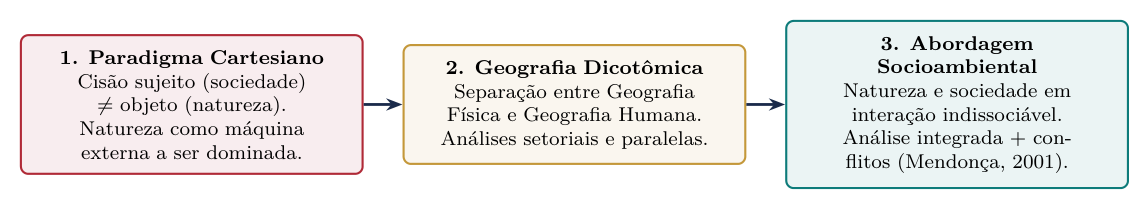
\includegraphics[width=0.92\textwidth]{figures/esquema_sociedade_natureza.png}
  \caption{Percurso histórico-epistemológico da ruptura cartesiana e da Geografia dicotômica até a emergência da abordagem socioambiental integrada (elaborado com base em Mendonça, 2001).}
  \label{fig:sociedade-natureza}
\end{figure}

\section{A Natureza como Construção Social e Histórica (Porto-Gonçalves, 2006)}

Nas páginas 8 a 36 de \emph{Os (des)caminhos do meio ambiente} (2006), Carlos Walter Porto-Gonçalves desenvolve uma tese central para a formação em Geografia, afirmando que \textbf{toda sociedade e toda cultura cria, inventa e institui uma determinada ideia do que seja a natureza}. Essa afirmação merece atenção rigorosa para evitar leituras simplistas. Reconhecer que a natureza é uma \emph{construção social e histórica} afirma a existência material objetiva da chuva, das rochas, da gravidade e dos processos biológicos, ao mesmo tempo em que destaca que o modo como os seres humanos percebem, classificam, valorizam e se relacionam com esses elementos varia profundamente ao longo da história e entre diferentes culturas.

Ao longo do tempo, diferentes matrizes histórico-culturais instituíram concepções distintas de natureza com expressões espaciais próprias (Porto-Gonçalves, 2006, p. 8--36). Em visões pré-modernas e entre povos indígenas e comunidades tradicionais brasileiras, rios, serras e matas constituem uma totalidade viva e um território de memória, pertencimento e reprodução comunitária, orientando manejos adaptados aos ciclos sazonais, como as áreas de uso comum no Semiárido (Figura~\ref{fig:potigua_cap2}).

\begin{figure}[H]
  \centering
  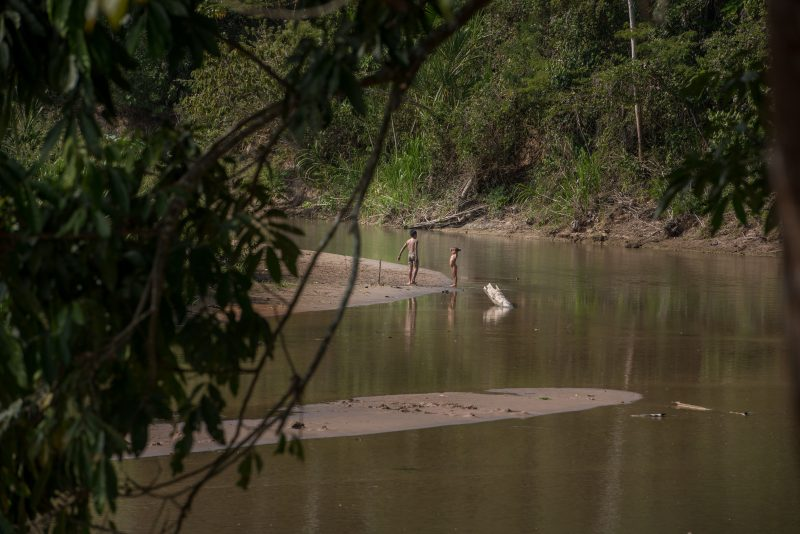
\includegraphics[width=0.76\textwidth]{figures/potigua.jpg}
  \caption{Território indígena e tradicional, expressando a natureza como espaço de vida, memória e pertencimento coletivo. Fonte: Acervo didático CHF662.}
  \label{fig:potigua_cap2}
\end{figure}

Em contraste histórico com essa territorialidade, a modernidade cartesiana e industrial concebeu a natureza como máquina externa e estoque mensurável de recursos sob dominação técnica contínua, multiplicando grandes obras, monoculturas, urbanização acelerada e frentes extrativas de alto impacto como a mineração industrial em larga escala (Figura~\ref{fig:grandes_minas_cap2}). Porto-Gonçalves (2006) aponta ainda um paradoxo revelador da modernidade, pois, paralelamente à devastação urbano-industrial, consolidou-se um preservacionismo excludente que romantiza a ``natureza intocada'' pela ausência humana e cria ilhas de proteção em conflito com moradores locais. Tanto o produtivismo quanto o preservacionismo excludente compartilham a raiz cartesiana que opõe sociedade e natureza como polos excludentes, fratura superada apenas pela perspectiva socioambiental crítica que articula materialidade biofísica, cultura, justiça territorial e convivência regional.

\begin{figure}[H]
  \centering
  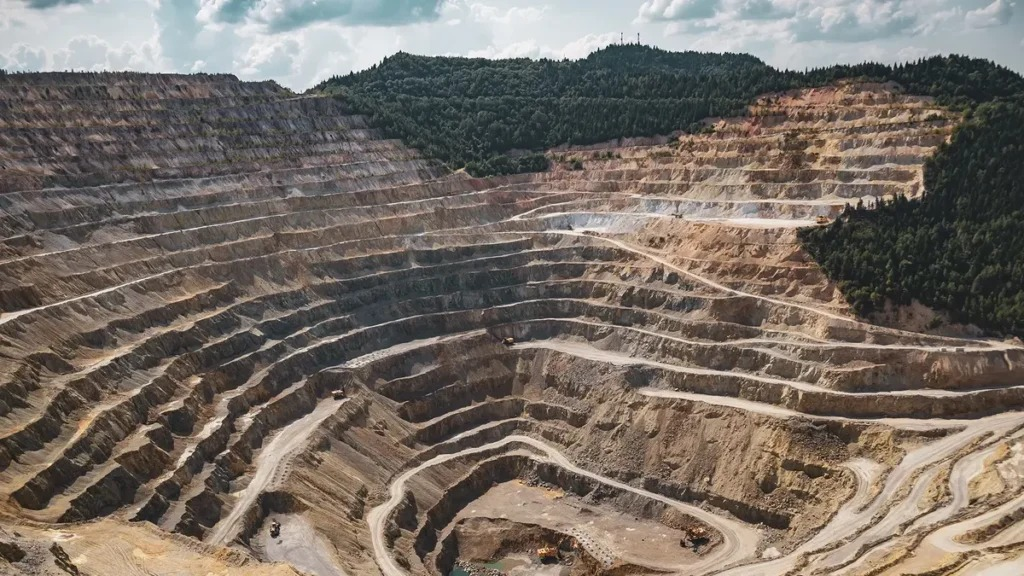
\includegraphics[width=0.76\textwidth]{figures/grandes_minas.jpg}
  \caption{Mineração industrial em larga escala, exemplificando a redução do relevo e do subsolo a mercadoria e estoque extrativo sob a racionalidade instrumental. Fonte: Acervo didático CHF662.}
  \label{fig:grandes_minas_cap2}
\end{figure}

O Exemplo 2.1 mostra como a concepção de ``natureza intocada'' reaparece em relatórios ambientais contemporâneos, reproduzindo o dualismo cartesiano.

\begin{boxExemplo}{2.1 (Básico)}{Identificando o Dualismo Cartesiano em um Relatório Ambiental}
\passoEnunciado{Para criar uma unidade de conservação de proteção integral em uma serra fictícia da Bahia \textit{(cenário didático ilustrativo)}, uma consultoria entregou um relatório técnico dividido em duas partes sem conexão. O Volume 1 descreve a flora e as nascentes como ``patrimônio natural puro'', e o Volume 2 recomenda a retirada imediata de 35 famílias que vivem há três gerações na área praticando extrativismo de baixa intensidade e manejo comunitário de pastagens, classificando qualquer presença humana como ``fator de destruição da natureza''.}
\passoDados{Relatório dividido em dois volumes isolados; idealização da área como ``natureza pura''; recomendação de remoção de 35 famílias tradicionais sem avaliar seus modos históricos de manejo.}
\passoPedido{Identificar qual concepção de natureza fundamenta o relatório à luz de Porto-Gonçalves (2006) e explicar por que essa postura reproduz o dualismo moderno.}
\passoMetodo{Análise epistemológica das concepções de natureza e do paradoxo preservacionista excludente em Porto-Gonçalves (2006, p. 8--36).}
\passoContas{%
\textbf{Passo 1, Concepção subjacente.} O relatório adota o mito da ``natureza intocada'', definindo o natural exclusivamente pela ausência de seres humanos.\\
\textbf{Passo 2, Raiz cartesiana (Porto-Gonçalves, 2006).} Embora aparente opor-se à exploração predatória, essa visão parte da mesma ruptura moderna que separa rigidamente sociedade e natureza em polos excludentes.\\
\textbf{Passo 3, Equívoco geográfico e social.} Ao tratar todas as formas de presença humana como igualmente destrutivas, a consultoria ignora que os modos de manejo tradicional dessas 35 famílias podem ter contribuído para conservar a cobertura vegetal e as nascentes ao longo de gerações, gerando um conflito socioambiental desnecessário.}
\passoResposta{O relatório fundamenta-se na concepção dicotômica da ``natureza intocada'', herdeira da ruptura cartesiana entre sociedade e natureza, ao opor automaticamente conservação ambiental e presença de populações tradicionais.}
\passoVerificacao{A crítica é coerente com a Análise Ambiental contemporânea, pois conservar nascentes exige avaliar empiricamente o impacto real de cada prática de uso da terra, diferenciando manejo comunitário de baixo impacto de pressões predatórias externas.}
\end{boxExemplo}

Ao estudar a tese de Porto-Gonçalves (2006), um equívoco recorrente consiste em interpretar a ideia de construção social como negação da realidade material dos processos naturais, conforme destacado no alerta a seguir.

\begin{boxErro}[Erro 2.1: Confundir ``Natureza como Construção Social'' com Negação da Materialidade Física]
\textbf{Equívoco frequente:} interpretar a tese de Porto-Gonçalves (2006) como se a erosão, as chuvas ou os processos geológicos fossem apenas ``invenções da mente humana'' sem realidade material.

\textbf{Por que está incorreto:} a materialidade biofísica existe objetivamente e obedece a leis físicas, químicas e biológicas. O que é social e historicamente construído é a \emph{ideia} de natureza, o significado cultural que lhe atribuímos e as formas técnicas e econômicas pelas quais a apropriamos e transformamos.

\textbf{Como evitar:} afirme sempre a dupla dimensão segundo a qual os processos naturais possuem dinâmica material própria, enquanto sua apropriação, valoração e interpretação são mediadas pela história e pela sociedade.
\end{boxErro}

\section{Apropriação dos Recursos Naturais e Racionalidade Instrumental}

Sob a modernidade capitalista, os elementos biofísicos da superfície terrestre passam por um processo sistemático de conversão em \textbf{recursos naturais}. Esse detalhe conceitual mostra-se decisivo na Geografia, pois a água, o vento, o solo ou um mineral existem independentemente da economia, adquirindo a condição de ``recursos'' quando um grupo social dispõe de técnica, demanda econômica e respaldo jurídico-político para se apropriar deles. Ao redigir diagnósticos ambientais, o(a) geógrafo(a) distingue três níveis operacionais interligados, começando pelo \textbf{elemento natural} em sua dinâmica biofísica (como o regime de ventos nas serras do Semiárido ou a água infiltrada em um aquífero), passando ao \textbf{recurso natural} quando incorporado por técnicas e finalidades sociais específicas (como o potencial eólico mapeado para geração elétrica ou a água captada para irrigação) e alcançando a condição de \textbf{mercadoria} quando esse recurso é apropriado privadamente e submetido à lógica de compra, venda e especulação. Grande parte dos conflitos socioambientais nasce quando um bem essencial à reprodução comunitária é transformado em mercadoria excludente.

Assim, a \textbf{apropriação dos recursos naturais} é guiada por uma \textbf{racionalidade instrumental} na qual a técnica é mobilizada para acelerar o giro do capital, ampliar a escala de extração e reduzir custos privados de produção. Disso decorre um descompasso estrutural entre duas temporalidades que governam o espaço geográfico (Figura~\ref{fig:temporalidades}). De um lado, o \textbf{tempo do capital}, rápido e linear, exige retorno financeiro em poucos anos, colheitas sucessivas, ampliação acelerada de redes energéticas e expansão contínua sobre novas fronteiras de terra e água. De outro lado, o \textbf{tempo da natureza}, lento e cíclico, envolve décadas para a regeneração florestal da Caatinga e do Cerrado, séculos para a formação de centímetros de solo fértil e ciclos plurianuais para a recarga de aquíferos subterrâneos.

\begin{figure}[H]
  \centering
  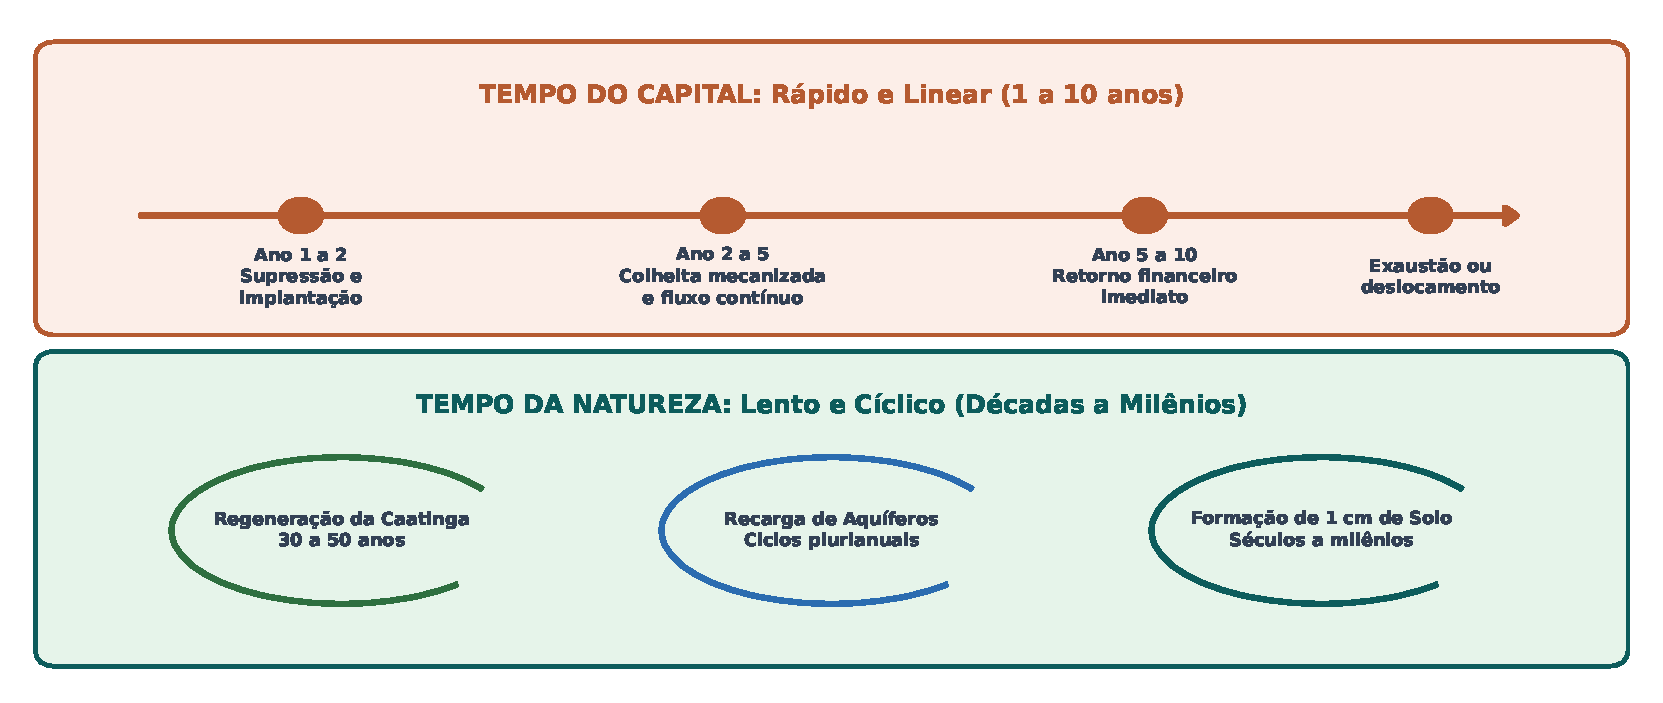
\includegraphics[width=0.94\textwidth]{figures/fig_cap02_temporalidades.pdf}
  \caption{Descompasso de temporalidades entre o tempo linear do capital (retorno em 1 a 10 anos) e o tempo cíclico da natureza (regeneração da Caatinga, recarga de aquíferos e pedogênese em décadas a milênios). Fonte: Elaboração didática CHF662 com base em Leff (2001) e Porto-Gonçalves (2006).}
  \label{fig:temporalidades}
\end{figure}

O Exemplo 2.2 ilustra como um elemento biofísico permanente no sertão baiano adquire o estatuto de recurso econômico e reconfigura relações fundiárias e ambientais.

\begin{boxExemplo}{2.2 (Básico)}{Da Natureza ao Recurso Natural: o Vento nas Serras do Semiárido}
\passoEnunciado{Durante décadas, os ventos intensos que sopram no topo de uma serra da Caatinga \textit{(cenário didático ilustrativo)} eram percebidos pelos moradores locais apenas como parte do clima cotidiano, influenciando a secagem do solo e o manejo dos rebanhos em áreas de uso comum. Nos últimos cinco anos, após o avanço de turbinas de grande porte, o mapeamento anemométrico e a instalação de uma subestação elétrica próxima, o mesmo vento passou a atrair grandes investimentos e contratos de arrendamento de terras para implantação de um complexo eólico.}
\passoDados{Elemento biofísico preexistente dado pelo regime de ventos intensos na serra; novos fatores históricos e técnicos envolvendo aerogeradores de grande porte, mapeamento de potencial eólico e proximidade de linhas de transmissão; consequência marcada por revalorização fundiária e contratos de arrendamento.}
\passoPedido{Explicar, com base na distinção entre \emph{elemento natural} e \emph{recurso natural}, por que o vento adquiriu valor econômico territorial apenas recentemente e quais tensões socioambientais podem emergir.}
\passoMetodo{Análise geográfica do processo de apropriação dos recursos naturais e da produção do espaço sob racionalidade instrumental.}
\passoContas{%
\textbf{Passo 1, De elemento natural a recurso.} O vento sempre existiu fisicamente na serra, mas só se converteu em \emph{recurso energético} quando condições técnicas (aerogeradores), infraestruturais (linhas de transmissão) e econômicas (mercado de energia) permitiram sua apropriação rentável.\\
\textbf{Passo 2, Reconfiguração espacial.} A implantação das torres exige estradas de acesso largas, bases de concreto e faixas de servidão, o que altera a cobertura de Caatinga, expõe o solo à erosão na base das torres e interfere na avifauna.\\
\textbf{Passo 3, Tensões socioambientais emergentes.} O cercamento de áreas antes usadas coletivamente, a assimetria na negociação de contratos de arrendamento e o desconforto acústico próximo às moradias transformam um projeto de ``energia renovável'' em arena de conflito territorial quando falta planejamento socioambiental justo.}
\passoResposta{O vento tornou-se recurso natural apenas quando incorporado por um conjunto técnico, infraestrutural e econômico específico; sua apropriação reorganiza o território da serra e pode gerar impactos físicos e conflitos fundiários com comunidades locais.}
\passoVerificacao{O exemplo antecipa uma lição-chave para a viagem de campo da Semana 11 (eixo de Canudos), mostrando que ser fonte renovável mantém a necessidade de avaliar impactos ambientais e conflitos territoriais.}
\end{boxExemplo}

\section{Conflitos Socioambientais e Produção do Espaço na Bahia e no Nordeste}

A apropriação desigual dos recursos naturais nunca ocorre em um espaço vazio. Todo território já é ocupado, manejado e significado por diferentes grupos sociais (comunidades camponesas, quilombolas, indígenas, pescadores artesanais, agricultores familiares, moradores urbanos, empresas e Estado). Quando um empreendimento ou política altera a qualidade do solo, o regime das águas, o acesso à terra ou o modo de vida local em benefício de determinados agentes e em prejuízo de outros, emergem \textbf{conflitos socioambientais}. Um conflito socioambiental constitui uma disputa concreta pela \textbf{produção do espaço geográfico}, na qual diferentes atores defendem usos incompatíveis ou assimétricos para o mesmo território. No Nordeste brasileiro e no estado da Bahia, quatro frentes territoriais exemplificam essa dinâmica.

Na frente de \textbf{expansão energética} no Semiárido Baiano, a combinação entre ventos constantes nas serras e chapadas, topografia favorável e proximidade de linhas de transmissão transformou áreas de Caatinga e espaços de uso rural em polos eólicos e solares (tema direto da Viagem de Campo da Semana~11). Embora apresentadas como fontes limpas de carbono, essas instalações modificam a paisagem imediata das comunidades rurais ao inserir aerogeradores de grande porte junto a moradias e cercados familiares (Figura~\ref{fig:parque_eolico_rural}), além de envolver supressão vegetal para plataformas e parques fotovoltaicos extensivos (Figura~\ref{fig:solar_desmatamento}), abertura de acessos pesados, compactação e erosão na base das torres, ruído contínuo e contratos assimétricos de arrendamento com famílias de fundo de pasto.

\begin{figure}[H]
  \centering
  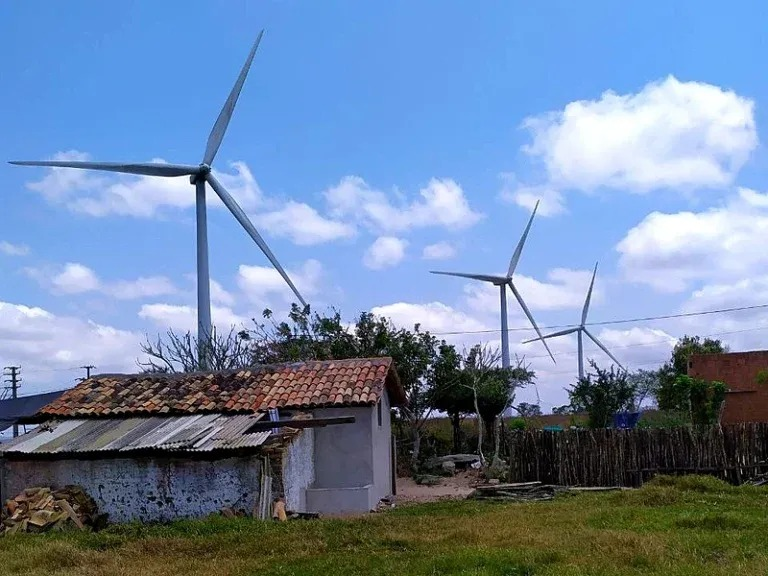
\includegraphics[width=0.76\textwidth]{figures/foto_parque_eolico_rural.jpg}
  \caption{Aerogeradores instalados em proximidade direta a moradias rurais no Semiárido, ilustrando a convivência cotidiana entre infraestruturas energéticas, ruído e organização espacial camponesa. Fonte: Acervo didático CHF662.}
  \label{fig:parque_eolico_rural}
\end{figure}

\begin{figure}[H]
  \centering
  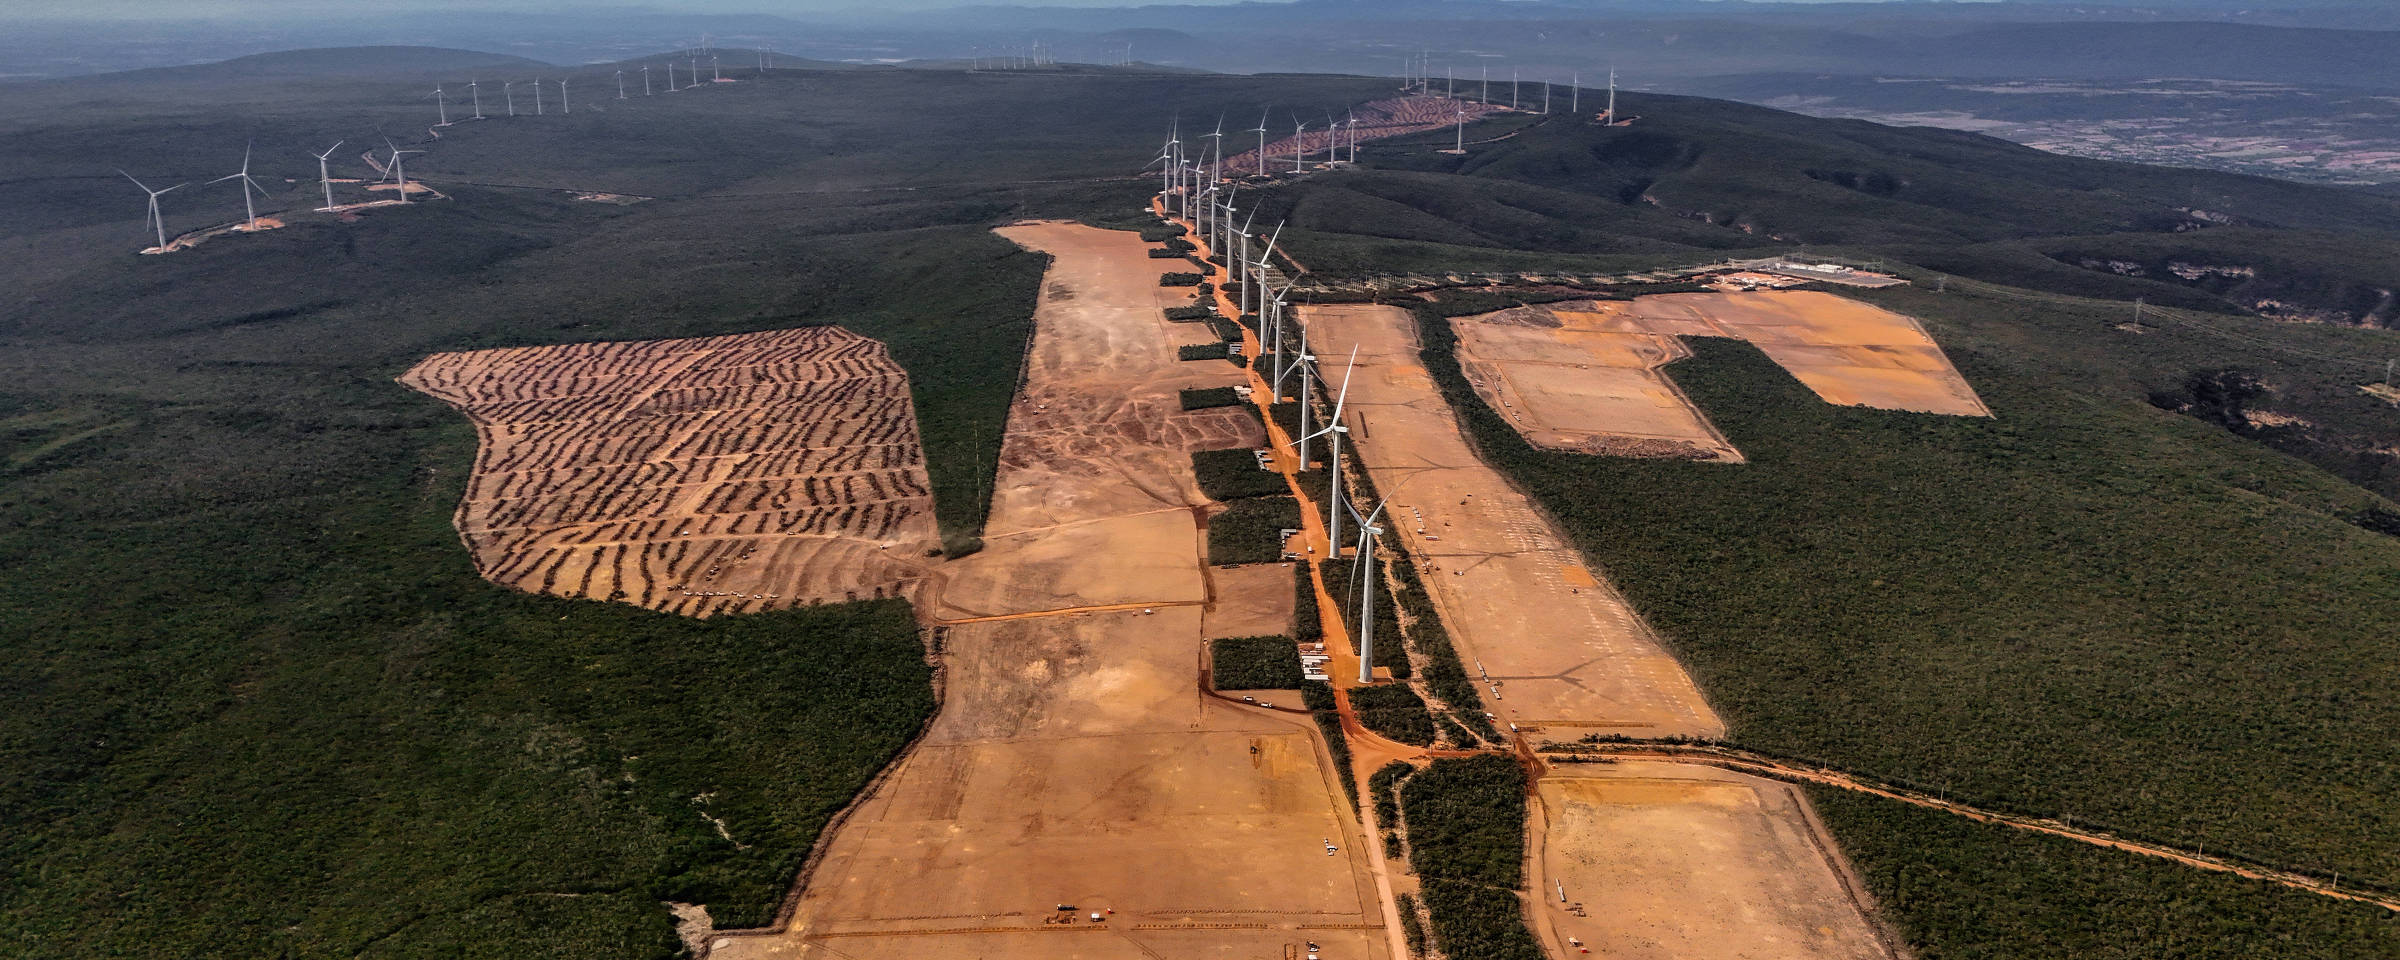
\includegraphics[width=0.76\textwidth]{figures/solar_desmatamento.jpg}
  \caption{Supressão da vegetação nativa associada à implantação de infraestrutura energética no Semiárido, evidenciando alterações na cobertura superficial e na dinâmica erosiva. Fonte: Acervo didático CHF662.}
  \label{fig:solar_desmatamento}
\end{figure}

Na frente das \textbf{barragens e grandes empreendimentos hídricos}, a construção de reservatórios de grande porte e projetos de regularização fluvial no Nordeste e na bacia do rio São Francisco, como a UHE Sobradinho (Figura~\ref{fig:sobradinho_barragem}), reconfigurou profundamente vales inteiros. Ao lado da geração hidrelétrica e da oferta de água para polos irrigados, esses empreendimentos implicaram o alagamento de terras férteis de vazante, o deslocamento compulsório de populações ribeirinhas, a alteração do pulso natural de cheias e vazantes e mudanças na dinâmica hidrossedimentológica a jusante, afetando a pesca artesanal e acelerando a erosão marginal.

\begin{figure}[H]
  \centering
  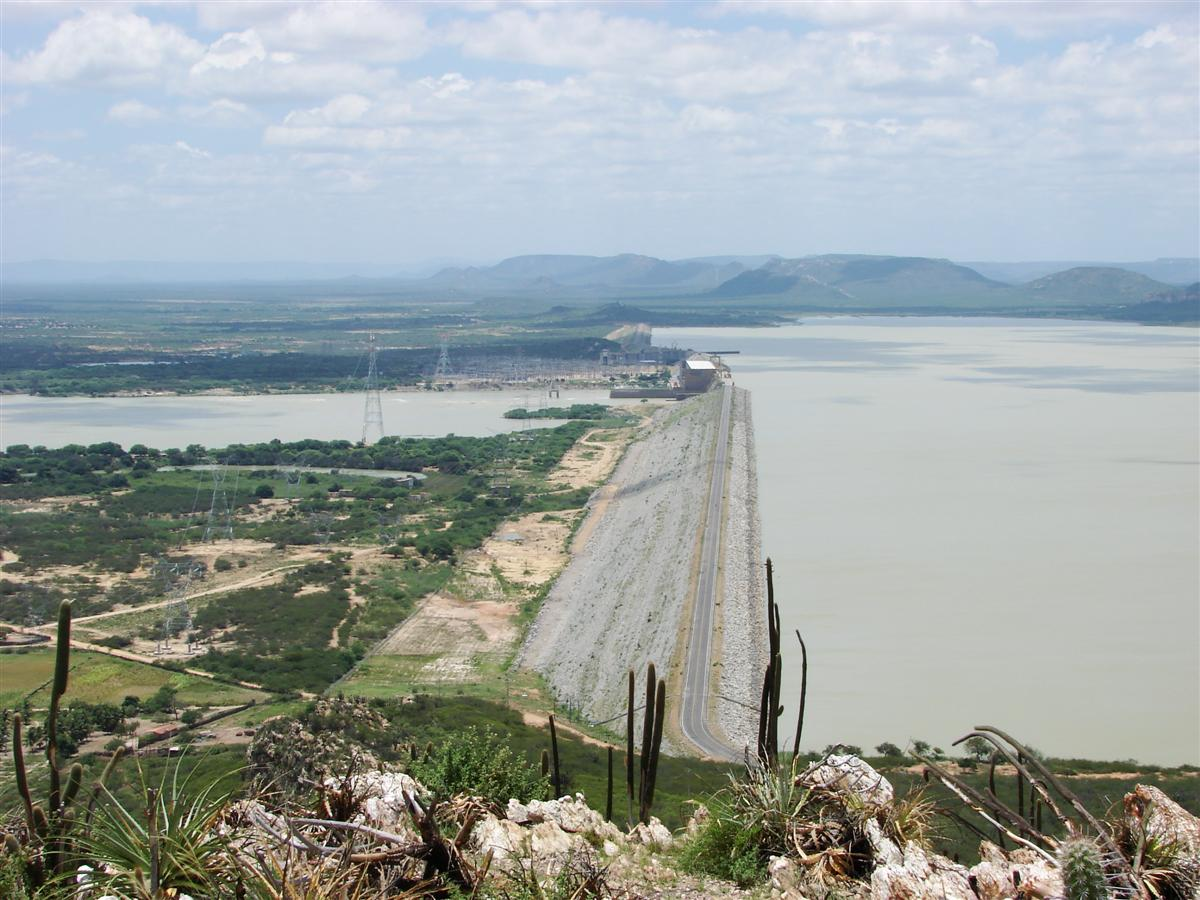
\includegraphics[width=0.76\textwidth]{figures/Barragem_de_Sobradinho-BA.jpg}
  \caption{Barragem da Usina Hidrelétrica de Sobradinho no Rio São Francisco (BA), marco da regularização de vazões e da reorganização territorial do vale. Fonte: Acervo didático CHF662.}
  \label{fig:sobradinho_barragem}
\end{figure}

Para compreender quantitativamente como disputas pela água em reservatórios expressam apropriação desigual, o Exemplo 2.3 analisa um balanço volumétrico simplificado em um açude comunitário.

\begin{boxExemplo}{2.3 (Intermediário)}{Balanço Hídrico Didático e Conflito Socioambiental em Açude Semiárido}
\passoEnunciado{Em uma microbacia semiárida fictícia \textit{(cenário didático ilustrativo)}, um açude público possui volume útil estimado de $120.000\text{ m}^3$ ao final da estação chuvosa, destinado a atender à demanda de 8 meses de estiagem (240 dias). O reservatório abastece 250 famílias de agricultores familiares (consumo médio estimado de $0{,}5\text{ m}^3/\text{dia}$ por família para usos domésticos e dessedentação de pequenos animais) e também passou a sofrer captação de um empreendimento privado de irrigação intensiva instalado a montante, que demanda $450\text{ m}^3/\text{dia}$. Desconsidere, neste exercício inicial, a evaporação direta para focar no balanço das demandas humanas.}
\passoDados{Volume útil disponível $V_{\text{disp}} = 120.000\text{ m}^3$; período de estiagem $T = 240\text{ dias}$; demanda comunitária de $250\text{ famílias} \times 0{,}5\text{ m}^3/(\text{família}\cdot\text{dia})$; demanda do empreendimento privado de $450\text{ m}^3/\text{dia}$.}
\passoPedido{Calcular a demanda total de cada grupo nos 240 dias, verificar se o volume disponível suporta ambos os usos simultaneamente e interpretar o resultado como um conflito socioambiental pelo acesso à água.}
\passoMetodo{Cálculo passo a passo de balanço volumétrico simples ($V = Q \times T$) articulado à análise geográfica de conflitos socioambientais e racionalidade instrumental.}
\passoContas{%
\textbf{Passo 1, Demanda diária e total das 250 famílias comunitárias.}
\[
Q_{\text{fam}} = 250 \times 0{,}5 = 125\text{ m}^3/\text{dia} \qquad\qquad V_{\text{fam}} = 125\text{ m}^3/\text{dia} \times 240\text{ dias} = 30.000\text{ m}^3
\]
\textbf{Passo 2, Demanda total do empreendimento privado de irrigação.}
\[
V_{\text{priv}} = 450\text{ m}^3/\text{dia} \times 240\text{ dias} = 108.000\text{ m}^3
\]
\textbf{Passo 3, Demanda conjunta e saldo hídrico.}
\[
V_{\text{total}} = V_{\text{fam}} + V_{\text{priv}} = 30.000 + 108.000 = 138.000\text{ m}^3
\]
\[
\text{Saldo} = V_{\text{disp}} - V_{\text{total}} = 120.000 - 138.000 = -18.000\text{ m}^3 \quad (\text{déficit de } 18.000\text{ m}^3)
\]
\textbf{Passo 4, Participação percentual nas demandas.} As 250 famílias respondem por $\frac{30.000}{138.000} \times 100\% \approx 21{,}7\%$ da demanda total (consumindo apenas $25\%$ do volume útil do açude), enquanto o único empreendimento privado responde por $\frac{108.000}{138.000} \times 100\% \approx 78{,}3\%$ (exigindo sozinho $90\%$ de toda a água armazenada).\\
\textbf{Passo 5, Interpretação socioambiental.} O déficit de $18.000\text{ m}^3$ decorre da apropriação concentrada do recurso sob racionalidade instrumental, uma vez que o açude atenderia quatro vezes a necessidade básica das 250 famílias. Como a evaporação real no Semiárido reduziria ainda mais o volume disponível, o colapso do abastecimento humano ocorreria antes do fim dos 240 dias.}
\passoResposta{As demandas somam $138.000\text{ m}^3$ frente a $120.000\text{ m}^3$ disponíveis, gerando déficit de $18.000\text{ m}^3$. O empreendimento privado concentra $78{,}3\%$ da demanda, caracterizando um conflito socioambiental distributivo pelo uso da água.}
\passoVerificacao{A soma $30.000 + 108.000 = 138.000\text{ m}^3$ confirma o déficit; pela Política Nacional de Recursos Hídricos (Lei nº 9.433/1997), em situações de escassez, o uso prioritário dos recursos hídricos é o consumo humano e a dessedentação de animais, reforçando a ilegitimidade de sacrificar o abastecimento das 250 famílias.}
\end{boxExemplo}

Reduzir conflitos distributivos desse tipo a problemas de comunicação impede o reconhecimento das relações de poder envolvidas, como aponta o alerta seguinte.

\begin{boxErro}[Erro 2.2: Tratar Conflitos Socioambientais como ``Falta de Diálogo'' ou ``Resistência ao Progresso'']
\textbf{Equívoco frequente:} explicar a oposição de comunidades rurais ou ribeirinhas a grandes obras (barragens, parques energéticos, fronteira agrícola) como ``desinformação'' ou ``atraso cultural''.

\textbf{Por que está incorreto:} conflitos socioambientais expressam disputas concretas e legítimas por água, solo, território, saúde e reprodução social. Rotular populações afetadas como ``contra o progresso'' oculta assimetrias de poder e a distribuição desigual de custos e benefícios.

\textbf{Como evitar:} identifique em todo conflito os atores envolvidos, os recursos disputados, os impactos físico-bióticos diferenciados e os projetos de território em confronto.
\end{boxErro}

Na terceira frente, relativa à \textbf{fronteira agrícola do Oeste Baiano} sob o domínio do Cerrado, a expansão acelerada da agricultura mecanizada intensiva sobre os chapadões (Figura~\ref{fig:pivos_matopiba}) reestruturou a economia regional e elevou a pressão sobre a vegetação nativa, sobre áreas estratégicas de recarga hídrica associadas ao sistema Aquífero Urucuia e sobre vazões de rios afluentes. Esse avanço desencadeou disputas territoriais pelo uso da terra e da água envolvendo comunidades tradicionais geraizeiras e de fecho de pasto nos fundos de vale.

\begin{figure}[H]
  \centering
  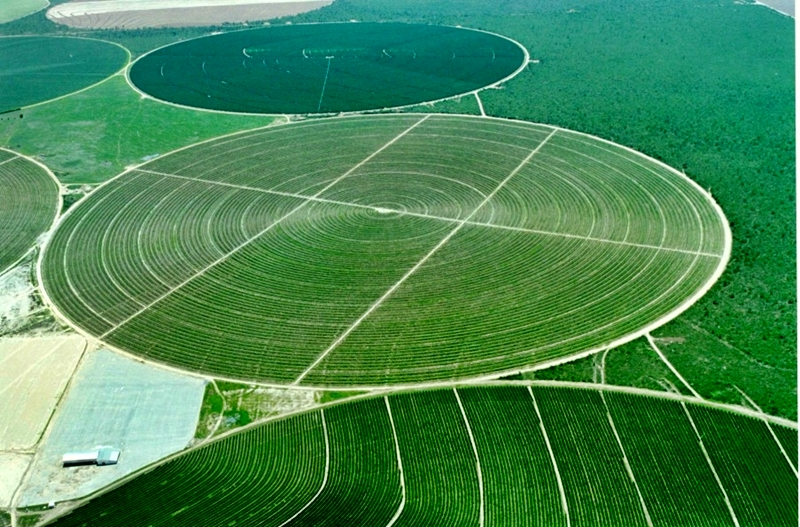
\includegraphics[width=0.76\textwidth]{figures/pivos_matopiba_cerrado.jpg}
  \caption{Irrigação com pivôs centrais no Cerrado do MATOPIBA, expressando a conversão intensiva das áreas de recarga em chapadões. Fonte: Acervo didático CHF662.}
  \label{fig:pivos_matopiba}
\end{figure}

Na quarta frente, associada ao \textbf{acesso desigual à água e à permanência territorial no Semiárido}, políticas historicamente centradas no ``combate à seca'' privilegiaram grandes açudes e obras concentradas em propriedades privadas, mantendo populações rurais dependentes de carros-pipa em estiagens. Em resposta a essa lógica concentradora, comunidades quilombolas (Figura~\ref{fig:quilombo_territorio}), associações rurais, movimentos sociais e universidades vêm consolidando estratégias de \textbf{convivência com o Semiárido}, articulando organização comunitária, tecnologias sociais descentralizadas de captação de água de chuva e manejo conservacionista do solo. O Exemplo 2.4 analisa a conectividade física e social entre chapadões convertidos e vales ocupados por comunidades tradicionais no Cerrado Baiano.

\begin{figure}[H]
  \centering
  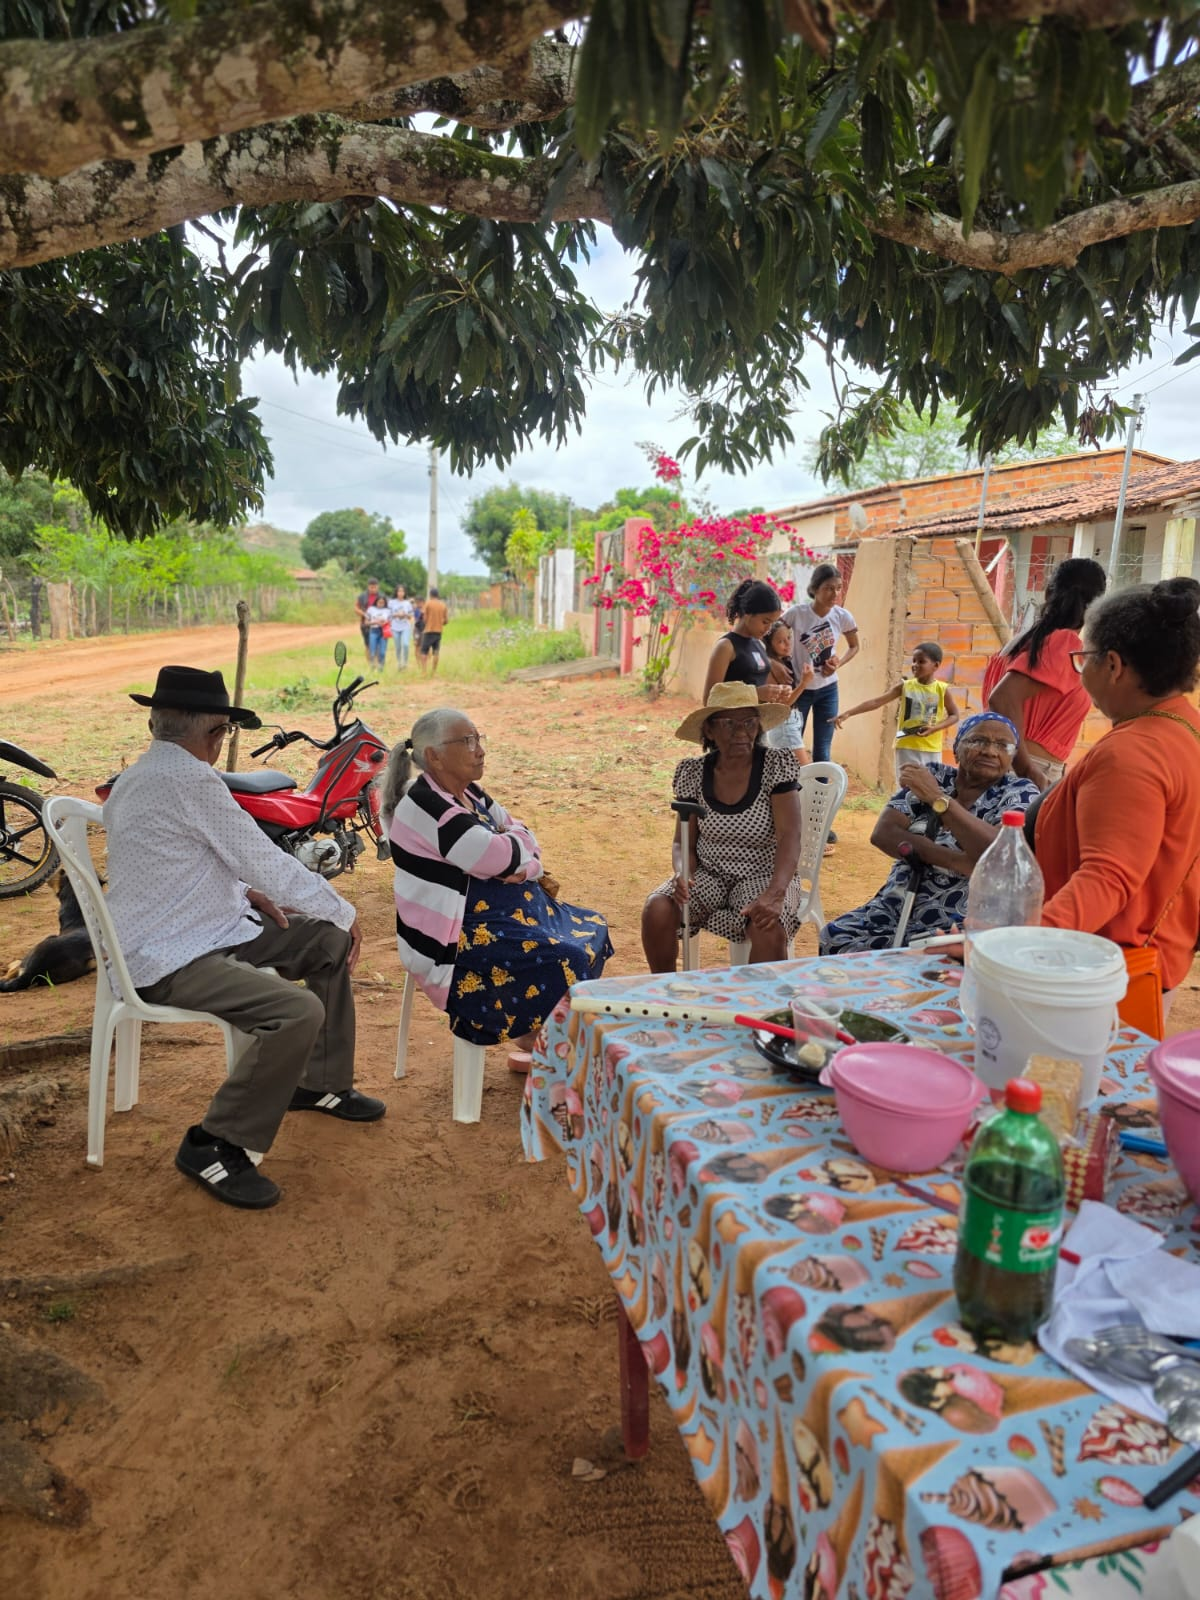
\includegraphics[width=0.76\textwidth]{figures/foto_quilombo_territorio.jpg}
  \caption{Comunidade quilombola de Tranqueira (BA), representando territorialidade tradicional, permanência comunitária e manejo adaptado ao ambiente semiárido. Fonte: Projeto Catuxe/UEFS.}
  \label{fig:quilombo_territorio}
\end{figure}

\begin{boxExemplo}{2.4 (Intermediário)}{Expansão da Fronteira Agrícola e Abordagem Socioambiental no Cerrado Baiano}
\passoEnunciado{Em uma sub-bacia fictícia de chapadão no Oeste Baiano \textit{(cenário didático ilustrativo)}, com área total de $40.000\text{ ha}$, o mapeamento de cobertura vegetal mostrou que, em 15 anos, a vegetação nativa de Cerrado reduziu-se de $32.000\text{ ha}$ para $14.000\text{ ha}$, substituída por lavouras mecanizadas irrigadas por pivôs centrais. Paralelamente, comunidades de fecho de pasto situadas nos vales a jusante relatam redução na vazão de veredas que utilizavam para cultivo de subsistência e criação extensiva.}
\passoDados{Área da sub-bacia de $40.000\text{ ha}$; Cerrado nativo reduzido de $32.000\text{ ha}$ para $14.000\text{ ha}$ em 15 anos; expansão de pivôs centrais no topo do chapadão; redução de vazão em veredas usadas por comunidades de fecho de pasto a jusante.}
\passoPedido{Calcular a área convertida e o percentual da sub-bacia que perdeu vegetação nativa nesse intervalo, construindo uma leitura integrada do caso segundo a Geografia Socioambiental de Mendonça (2001).}
\passoMetodo{Quantificação da conversão de cobertura vegetal seguida de análise dialética entre dinâmica físico-hidrológica (recarga no chapadão e descarga nas veredas) e conflito territorial (Mendonça, 2001).}
\passoContas{%
\textbf{Passo 1, Quantificação da perda de Cerrado.} A variação absoluta é $\Delta A = 14.000 - 32.000 = -18.000\text{ ha}$, correspondendo a $\frac{18.000}{40.000} \times 100\% = 45{,}0\%$ da sub-bacia e a $\frac{18.000}{32.000} \times 100\% = 56{,}25\%$ do Cerrado existente no início do período.\\
\textbf{Passo 2, Leitura físico-hidrológica integrada.} Os chapadões arenosos do Cerrado funcionam como áreas estratégicas de infiltração e recarga subterrânea que alimentam nascentes e veredas nos vales. A conversão de $45\%$ da sub-bacia associada à captação intensiva por pivôs centrais altera o balanço hídrico local e reduz a contribuição para os cursos d'água a jusante.\\
\textbf{Passo 3, Leitura socioambiental (Mendonça, 2001).} Enquanto uma leitura puramente física mediria apenas a vazão das veredas e uma abordagem puramente social descreveria apenas a disputa fundiária, a Geografia Socioambiental une ambos os planos ao evidenciar que a produção do espaço pelo agronegócio intensivo no topo da bacia transfere custos hídricos e vulnerabilidade social para as comunidades tradicionais nos fundos de vale.}
\passoResposta{Foram convertidos $18.000\text{ ha}$ ($45{,}0\%$ da sub-bacia e $56{,}25\%$ do Cerrado inicial). Sob a Geografia Socioambiental (Mendonça, 2001), o rebaixamento das veredas evidencia a inseparabilidade entre conectividade hidrológica chapadão-vale e apropriação desigual do território.}
\passoVerificacao{Os cálculos fecham ($32.000 - 18.000 = 14.000\text{ ha}$, restando $35\%$ da sub-bacia com Cerrado nativo), e a interpretação respeita a lógica de bacia hidrográfica ao conectar uso do solo em área de recarga com impactos socioespaciais a jusante.}
\end{boxExemplo}

Reconhecer o papel das comunidades tradicionais na conservação de veredas e áreas de uso comum previne o erro clássico de igualar toda presença humana à degradação ambiental.

\begin{boxErro}[Erro 2.3: Reproduzir o Mito da ``Natureza Intocada'' na Conservação Ambiental]
\textbf{Equívoco frequente:} supor que toda presença humana degrada o ambiente na mesma medida e que conservar significa necessariamente esvaziar territórios de seus habitantes tradicionais.

\textbf{Por que está incorreto:} como aponta Porto-Gonçalves (2006), essa postura reproduz a cisão cartesiana entre humano e natural, equiparando sistemas comunitários de baixo impacto a empreendimentos industriais de alta degradação.

\textbf{Como evitar:} analise empiricamente as práticas reais de uso da terra e reconheça que populações tradicionais frequentemente atuam como guardiãs da sociobiodiversidade.
\end{boxErro}

\section{Introdução à Abordagem Socioambiental na Geografia (Mendonça, 2001)}

Diante das limitações do dualismo cartesiano e da intensidade dos conflitos territoriais contemporâneos, a Geografia brasileira desenvolveu esforços consistentes para superar a separação entre o estudo da natureza e o estudo da sociedade. Um marco de referência desse movimento é o artigo \emph{Geografia socioambiental}, publicado por Francisco Mendonça na revista \emph{Terra Livre} (n. 16, 2001, p. 139--158). Mendonça (2001) questiona o uso genérico do termo ``ambiental'' quando reduzido exclusivamente à esfera natural (relevo, clima, fauna e flora) sem incorporar sujeitos históricos, desigualdade social e relações de poder. Por isso, o autor defende a adoção deliberada do prefixo \textbf{``socio-''} na expressão \textbf{Geografia Socioambiental}, afirmando desde a própria denominação que os problemas ambientais só podem ser compreendidos na interação dialética entre natureza e sociedade.

Essa introdução à abordagem socioambiental estabelece princípios metodológicos que serão aprofundados no Capítulo~3. A \textbf{superação da dicotomia físico-humana} articula as especificidades da geomorfologia, da climatologia e da geografia agrária diante de problemas concretos em que processos naturais e sociais se coproduzem. A \textbf{centralidade da sociedade na problemática ambiental} reconhece que enchentes urbanas, erosão acelerada, desertificação ou escassez hídrica atingem os grupos sociais de forma desigual conforme a vulnerabilidade e a organização do espaço. Além disso, o \textbf{compromisso com o diagnóstico e a intervenção territorial} combina rigor teórico-metodológico e relevância social para subsidiar políticas públicas, licenciamento, regras de alocação de água e recuperação de áreas degradadas. Esses quatro eixos, compreendendo a ruptura cartesiana na modernidade, a natureza como construção histórica (Porto-Gonçalves, 2006), os conflitos socioambientais na Bahia e no Nordeste e a abordagem socioambiental (Mendonça, 2001), formam a base direta para a elaboração do Estudo Orientado 1 (EO1) e conduzem à formalização do Sistema GTP no Capítulo~3.

% ----------------------------------------------------------------------------
% ETAPA 4 - SÍNTESE AVANÇADA E ESTUDO DE CASO INTEGRADOR
% ----------------------------------------------------------------------------
\etapa{4}{Síntese Avançada: Barragens, Temporalidades e Conflito Territorial}

Grandes obras de regularização fluvial oferecem um laboratório privilegiado para observar como a racionalidade instrumental, a imposição do tempo linear sobre os pulsos naturais e a desconsideração das territorialidades locais convergem no mesmo vale. O Exemplo 2.5 integra Porto-Gonçalves (2006) e Mendonça (2001) na avaliação socioambiental de uma barragem nordestina.

\begin{boxExemplo}{2.5 (Avançado)}{Barragem Fluvial, Descompasso de Temporalidades e Conflito Territorial}
\passoEnunciado{A construção de uma barragem de médio porte em um vale fluvial nordestino \textit{(cenário didático ilustrativo)} regularizou a vazão do rio para garantir geração elétrica e fornecimento constante a um perímetro agroindustrial. Cinco anos após o enchimento do reservatório, observam-se três efeitos encadeados, compreendendo a perda da prática secular de agricultura de vazante por comunidades ribeirinhas reassentadas em terrenos secos, a redução da deposição natural de nutrientes nas várzeas a jusante com intensificação da erosão marginal pela retenção de sedimentos no reservatório, e o declínio da pesca artesanal devido à barreira física à migração de peixes e à homogeneização do pulso de cheias.}
\passoDados{Obra de regularização fluvial voltada à geração elétrica e irrigação intensiva; três efeitos após 5 anos envolvendo perda da agricultura de vazante pós-reassentamento, retenção de sedimentos com erosão marginal a jusante e declínio da pesca artesanal.}
\passoPedido{Analisar o caso integrando a racionalidade instrumental e o descompasso entre tempo do capital e tempo ecológico, a concepção de natureza subjacente à obra (Porto-Gonçalves, 2006) e diretrizes de diagnóstico sob a ótica da Geografia Socioambiental (Mendonça, 2001).}
\passoMetodo{Síntese teórico-metodológica articulando Porto-Gonçalves (2006, p. 8--36), Mendonça (2001) e processos hidrossedimentológicos fluviais básicos.}
\passoContas{%
\textbf{Passo 1, Racionalidade instrumental e temporalidades.} O projeto tratou o rio sob o tempo linear e contínuo da produção industrial (vazão regularizada o ano inteiro), suprimindo o pulso sazonal de cheias e vazantes que estruturava tanto o ecossistema aquático (reprodução de peixes e renovação sedimentar das várzeas) quanto o calendário agrícola das famílias ribeirinhas.\\
\textbf{Passo 2, Concepção moderna de natureza (Porto-Gonçalves, 2006).} O rio foi concebido como tubulação hidráulica ou estoque de energia potencial a ser domado pela engenharia, ignorando que, para os ribeirinhos, ele constitui um território de vida historicamente construído. O reassentamento em terras secas pressupôs que qualquer lote substitui outro, apagando a especificidade ecológica e cultural da várzea.\\
\textbf{Passo 3, Diretrizes de diagnóstico socioambiental (Mendonça, 2001).} Um diagnóstico rigoroso deve avaliar a bacia inteira (montante, reservatório e jusante) com balanço de sedimentos e estabilidade de margens, mapear territorialidades tradicionais e dependência direta dos pulsos hidrológicos antes do licenciamento, e propor regras de vazões ambientais (hidrograma ecológico) acompanhadas de reparação territorial e participação comunitária na gestão do reservatório.}
\passoResposta{O caso evidencia como a racionalidade instrumental transforma um sistema fluvial vivo em infraestrutura setorial, rompendo simultaneamente processos hidrossedimentológicos e modos de vida ribeirinhos; a Geografia Socioambiental exige diagnosticar a bacia de forma integrada e reconhecer os sujeitos territoriais afetados.}
\passoVerificacao{A análise confirma a interdependência entre físico e social, pois a retenção de sedimentos pela barragem gera erosão marginal a jusante, empobrece várzeas e compromete a segurança alimentar e a renda das comunidades.}
\end{boxExemplo}

% ----------------------------------------------------------------------------
% ETAPA 5 - ARMADILHA CONCEITUAL E MATERIAIS AUDIOVISUAIS DE APOIO
% ----------------------------------------------------------------------------
\etapa{5}{Armadilha Conceitual e Materiais Audiovisuais de Apoio}

Ao aplicar a Geografia Socioambiental em trabalhos acadêmicos e relatórios técnicos, um erro frequente consiste em justapor capítulos independentes sobre o meio físico e a sociedade, mantendo intacta a cisão cartesiana sob nova nomenclatura.

\begin{boxErro}[Erro 2.4: Reduzir a Geografia Socioambiental à Justaposição de Física e Humana]
\textbf{Equívoco frequente:} acreditar que aplicar Mendonça (2001) consiste em escrever uma seção sobre clima e solo e outra seção independente sobre população e economia.

\textbf{Por que está incorreto:} justapor capítulos paralelos mantém intacta a dicotomia clássica da Geografia. A abordagem socioambiental exige mostrar como processos naturais e dinâmicas sociais interagem e se modificam reciprocamente no mesmo espaço.

\textbf{Como evitar:} formule suas análises a partir de nexos causais integrados, explicando como o modelo de ocupação de uma encosta ou bacia altera processos erosivos e concentra riscos sobre grupos vulneráveis.
\end{boxErro}

Para aprofundar os temas históricos e conceituais da relação sociedade-natureza na modernidade, assista às videoaulas indicadas na página da disciplina, iniciando por \textit{Relações de apropriação e transformação da natureza pelas sociedades humanas} (\url{https://www.youtube.com/watch?v=HX13IX_4290}) e complementando com \textit{Gestão Ambiental - Conceitos e Evolução das questões ambientais} (\url{https://www.youtube.com/watch?v=9eDzntrUvHY}), que contextualizam a trajetória histórica do pensamento ambiental e os modos de apropriação territorial.

% ----------------------------------------------------------------------------
% ETAPA 6 - EXERCÍCIOS DE FIXAÇÃO
% ----------------------------------------------------------------------------
\etapa{6}{EXERCÍCIOS DE FIXAÇÃO}

\subsection*{Nível 1: Básicos (Compreensão Conceitual)}

\begin{enumerate}[leftmargin=1.8em, itemsep=4pt]
  \item Explique em que consiste a \emph{ruptura cartesiana} entre sociedade e natureza na modernidade e aponte uma consequência direta dessa cisão para a organização da Geografia clássica.
  \espacoResolucao[1.8cm]

  \item Com base em Porto-Gonçalves (2006, p. 8--36), esclareça o significado da afirmação de que a natureza é uma \emph{construção social e histórica}, cuidando para preservar o reconhecimento da materialidade dos processos físicos.
  \espacoResolucao[1.8cm]

  \item Diferencie \emph{elemento natural} de \emph{recurso natural}, ilustrando com um exemplo concreto da realidade baiana ou nordestina.
  \espacoResolucao[1.8cm]

  \item Explique o descompasso entre o \emph{tempo do capital} e o \emph{tempo da natureza} no contexto da racionalidade instrumental moderna.
  \espacoResolucao[1.8cm]

  \item Segundo Francisco Mendonça (2001), qual é a justificativa teórica e metodológica para o uso do prefixo ``socio-'' na expressão \emph{Geografia Socioambiental}?
  \espacoResolucao[1.8cm]

\subsection*{Nível 2: Intermediários (Análise Crítica e Aplicação)}

  \item Analise o paradoxo apontado por Porto-Gonçalves (2006) entre a exploração predatória da natureza como mercadoria e a defesa de uma ``natureza intocada'' sem presença humana. O que essas duas visões têm em comum?
  \espacoResolucao[1.8cm]

  \item Escolha uma das quatro frentes de conflito socioambiental discutidas no capítulo (expansão energética no Semiárido, barragens fluviais, fronteira agrícola no Oeste Baiano ou acesso desigual à água) e identifique o recurso apropriado, os principais atores em disputa e dois impactos físico-bióticos articulados a efeitos sociais.
  \espacoResolucao[1.8cm]

  \item Em um cenário didático ilustrativo, um reservatório comunitário no Semiárido dispõe de $90.000\text{ m}^3$ de volume útil para 200 dias de estiagem. Duas demandas disputam essa água, sendo 150 famílias que consomem $0{,}6\text{ m}^3/\text{dia}$ cada e um empreendimento externo que solicita autorização para captar $400\text{ m}^3/\text{dia}$. Calcule a demanda total de cada parte no período, verifique se há déficit e analise o caso sob a ótica dos conflitos socioambientais.
  \espacoResolucao[1.8cm]

  \item Diferencie as políticas históricas de ``combate à seca'' das estratégias contemporâneas de ``convivência com o Semiárido'', relacionando essa distinção à racionalidade instrumental e à justiça socioambiental.
  \espacoResolucao[1.8cm]

  \item Elabore um parágrafo analítico demonstrando como a abordagem socioambiental (Mendonça, 2001) supera tanto o naturalismo redutor quanto o sociologismo que ignora o suporte físico-biótico do território.
  \espacoResolucao[1.8cm]

\subsection*{Nível 3: Aplicados e Objetivos (Múltipla Escolha)}

  \item Na análise de Porto-Gonçalves (2006, p. 8--36) sobre a formação histórica da questão ambiental na modernidade, a separação entre sociedade e natureza:
  \begin{alternativas}
    \item É uma característica biológica universal presente de forma idêntica em todas as culturas humanas desde a pré-história.
    \item Consolida-se historicamente com o pensamento moderno-cartesiano, instituindo a natureza como objeto externo e passivo a ser dominado pela ciência e pela técnica.
    \item Foi completamente superada pela Revolução Industrial, que reintegrou o ritmo produtivo das fábricas aos ciclos lentos dos ecossistemas.
    \item Refere-se exclusivamente à divisão administrativa entre zonas urbanas e zonas rurais nos municípios brasileiros.
    \item Impediu o desenvolvimento das ciências da natureza, pois o mecanicismo cartesiano rejeitava qualquer estudo matemático do mundo físico.
  \end{alternativas}
  \espacoResolucao[1.8cm]

  \item Sobre o processo pelo qual um elemento biofísico passa a ser tratado como \emph{recurso natural}, é \textbf{correto} afirmar que:
  \begin{alternativas}
    \item Todo elemento físico da crosta terrestre é automaticamente um recurso econômico, independentemente da técnica ou da organização social existente.
    \item A transformação de elementos da natureza em recursos naturais depende de condições técnicas, econômicas, culturais e políticas historicamente situadas.
    \item Recursos renováveis, como o vento e a energia solar, jamais geram impactos ambientais ou conflitos territoriais quando apropriados em larga escala.
    \item A apropriação de recursos naturais sob racionalidade instrumental respeita integralmente o tempo geológico de formação dos solos e de recarga dos aquíferos.
    \item A noção de recurso natural é neutra e alheia às disputas fundiárias ou à produção do espaço geográfico.
  \end{alternativas}
  \espacoResolucao[1.8cm]

  \item No contexto da Bahia e do Nordeste, a expansão de parques eólicos em áreas serranas da Caatinga exemplifica um conflito socioambiental porque:
  \begin{alternativas}
    \item A geração eólica produz grandes volumes de gases de efeito estufa diretamente na atmosfera do Semiárido durante a rotação das pás.
    \item Embora utilize fonte renovável, a apropriação espacial das serras provoca supressão vegetal, erosão na base das torres, interferência na avifauna e tensões fundiárias com comunidades locais.
    \item Os ventos do Semiárido são insuficientes para movimentar turbinas, tornando a região tecnicamente inviável para energia eólica.
    \item As comunidades locais opõem-se por princípio a qualquer forma de energia elétrica, recusando-se a utilizar eletricidade em suas residências.
    \item Os impactos físicos das obras restringem-se ao interior das subestações urbanas, sem atingir o relevo, os solos ou a vegetação da Caatinga.
  \end{alternativas}
  \espacoResolucao[1.8cm]

  \item De acordo com a proposta de \emph{Geografia Socioambiental} formulada por Francisco Mendonça (2001):
  \begin{alternativas}
    \item O estudo ambiental deve restringir-se aos fenômenos climáticos e geomorfológicos naturais, evitando interferência de temas sociais e políticos.
    \item A Geografia Física deve ser extinta dos cursos de graduação, pois apenas a análise econômica explica a degradação do espaço.
    \item A incorporação do termo ``socioambiental'' busca superar a dicotomia físico-humana, compreendendo o ambiente a partir da interação indissociável entre natureza e sociedade.
    \item Os desastres e a degradação ambiental atingem de maneira uniforme todas as classes sociais, independentemente da organização do território.
    \item A abordagem socioambiental consiste em anexar um capítulo de demografia ao final de relatórios geomorfológicos sem estabelecer relações causais entre eles.
  \end{alternativas}
  \espacoResolucao[1.8cm]

  \item Em um cenário didático ilustrativo, uma comunidade tradicional de fundo de pasto e uma empresa agroindustrial disputam o uso das águas de um riacho que nasce em área de chapadão. A análise desse episódio como \textbf{conflito socioambiental} exige reconhecer que:
  \begin{alternativas}
    \item Trata-se apenas de um mal-entendido de comunicação que desaparece assim que a empresa apresentar seu catálogo comercial.
    \item Existe confronto entre diferentes racionalidades, interesses e modos de apropriação do território e da água, com efeitos diretos sobre a dinâmica hidrológica e a reprodução social.
    \item O conflito só tem relevância geográfica se houver alteração na precipitação média anual registrada na estação meteorológica mais próxima.
    \item A solução técnica adequada consiste em transferir integralmente o controle da bacia ao agente de maior capacidade de investimento financeiro.
    \item A análise deve desconsiderar o uso do solo na área de recarga do chapadão, pois a questão pertence exclusivamente ao direito privado.
  \end{alternativas}
  \espacoResolucao[1.8cm]
\end{enumerate}

% ----------------------------------------------------------------------------
% ETAPA 7 - QUESTÕES DE PROVAS, ENADE E CONCURSOS AMBIENTAIS
% ----------------------------------------------------------------------------
\etapa{7}{QUESTÕES DE PROVAS, ENADE E CONCURSOS AMBIENTAIS}

\begin{enumerate}[leftmargin=1.8em, itemsep=5pt, start=16]
  \item \textbf{(Questão autoral, estilo ENADE / Concurso Ambiental)} Leia o excerto adaptado dos debates epistemológicos da Geografia contemporânea: \emph{``Toda sociedade, toda cultura cria, inventa, institui uma determinada ideia do que seja a natureza. Nesse sentido, o conceito de natureza é criado e instituído historicamente pelos seres humanos.''} (em diálogo com Porto-Gonçalves, 2006). Com base nessa perspectiva e na formação histórica da questão ambiental na modernidade, assinale a alternativa \textbf{correta}:
  \begin{alternativas}
    \item A afirmação nega a existência física de processos geomorfológicos e hidrológicos, reduzindo o meio ambiente a uma ficção linguística sem base material.
    \item A ideia moderna de natureza como objeto externo e dominável serviu de suporte ideológico à apropriação instrumental dos territórios e ao aprofundamento da crise ambiental.
    \item A concepção cartesiana promoveu a reunificação harmoniosa entre cultura, religião, ecossistemas locais e economia industrial desde o século XVII.
    \item O conceito de natureza permaneceu imutável desde a Antiguidade até o século XXI, alterando-se apenas a tecnologia empregada na agricultura.
    \item A defesa de áreas naturais completamente isoladas da ação humana rompe definitivamente com a dicotomia moderna entre sociedade e natureza.
  \end{alternativas}
  \espacoResolucao[1.8cm]

  \item \textbf{(Questão autoral, estilo ENADE / Concurso Ambiental)} Considere a implantação de grandes barragens e a expansão da fronteira agrícola mecanizada em bacias hidrográficas do Nordeste brasileiro. Sob a perspectiva da produção do espaço geográfico e da Geografia Socioambiental (Mendonça, 2001), analise as proposições abaixo:
  \begin{enumerate}[label=\Roman*., leftmargin=1.6em, itemsep=1.5pt]
    \item A regularização artificial de vazões por barragens pode alterar a dinâmica hidrossedimentológica a jusante e desestruturar modos de vida ribeirinhos baseados no pulso natural de cheias e vazantes.
    \item A conversão acelerada de vegetação nativa em áreas de recarga hídrica conecta processos físico-hidrológicos a conflitos territoriais com comunidades situadas nos vales a jusante.
    \item O descompasso entre o tempo acelerado de retorno do capital e o tempo lento de regeneração edáfica e hidrológica intensifica quadros de degradação e vulnerabilidade socioambiental.
    \item Por envolverem obras de infraestrutura autorizadas pelo Estado, grandes empreendimentos hídricos e agrícolas são tecnicamente neutros e não constituem conflitos socioambientais.
  \end{enumerate}
  Estão corretas apenas as proposições:
  \begin{alternativas}
    \item I e IV.
    \item II e IV.
    \item I, II e III.
    \item II, III e IV.
    \item I, III e IV.
  \end{alternativas}
  \espacoResolucao[1.8cm]

  \item \textbf{(Questão autoral, estilo ENADE / Concurso Ambiental)} Em um concurso para Geógrafo(a) de órgão ambiental estadual, solicitou-se a escolha da diretriz metodológica mais coerente com a abordagem socioambiental (Mendonça, 2001) para diagnosticar conflitos de uso da terra e escassez hídrica em uma bacia do Semiárido Baiano. A alternativa que atende rigorosamente a essa diretriz é:
  \begin{alternativas}
    \item Elaborar exclusivamente o mapeamento geomorfológico e climático da bacia, deixando as questões de acesso à água e posse da terra fora do escopo do relatório técnico.
    \item Adotar o enfoque de ``combate à seca'' baseado unicamente em obras hidráulicas concentradas, dispensando o diagnóstico da cobertura vegetal e das práticas comunitárias.
    \item Integrar o levantamento dos processos físico-bióticos (relevo, solos, vegetação e dinâmica hídrica) à análise das relações sociais, dos conflitos de uso dos recursos e das vulnerabilidades territoriais.
    \item Substituir o levantamento de campo e os indicadores físicos por entrevistas de opinião, pois a abordagem socioambiental considera dispensáveis os dados da Geografia Física.
    \item Aplicar o mesmo modelo produtivo mecanizado em toda a bacia para padronizar o uso do solo e eliminar diferenças culturais entre os moradores.
  \end{alternativas}
  \espacoResolucao[1.8cm]
\end{enumerate}

\begin{boxDica}[Orientações para o Estudo Orientado 1 (EO1) e a Prova Dissertativa]
O \textbf{EO1} (valor $0{,}5$ ponto, entregue na Semana 2) exige leitura atenta de \textbf{Porto-Gonçalves (2006, p. 8--36)} e introdução a \textbf{Mendonça (2001)}. Para produzir uma resposta sólida no EO1 e na Prova Teórica (Semana 10):
\begin{enumerate}[leftmargin=1.5em, itemsep=2pt]
  \item \textbf{Evite resumos descritivos soltos,} articulando explicitamente a cadeia que vai da modernidade e ruptura cartesiana até a conversão da natureza em mercadoria, os conflitos socioambientais e a resposta da Geografia Socioambiental.
  \item \textbf{Dê concretude geográfica,} exemplificando conflitos socioambientais com processos reais da Bahia e do Nordeste (eólicas no Semiárido, barragens, Oeste Baiano ou acesso à água), sem inventar dados estatísticos.
  \item \textbf{Use vocabulário preciso,} distinguindo \emph{elemento natural} de \emph{recurso natural}, diferenciando \emph{construção social da ideia de natureza} de negação da materialidade física e justificando o papel do prefixo ``socio-'' em Mendonça (2001).
\end{enumerate}
\end{boxDica}

% ----------------------------------------------------------------------------
% ETAPA 8 - GABARITO COMENTADO (PÁGINA SEPARADA)
% ----------------------------------------------------------------------------
\clearpage
\etapa{8}{GABARITO COMENTADO}

\begin{boxGabarito}[Resolução Comentada: Nível 1 (Questões 1 a 5)]
\begin{enumerate}[leftmargin=1.8em, itemsep=4pt]
  \item \textbf{Ruptura cartesiana e Geografia clássica.} A ruptura cartesiana separou o sujeito racional humano (\emph{res cogitans}, sociedade e cultura) da matéria externa (\emph{res extensa}, natureza), concebendo a natureza como máquina passiva a ser dominada pela ciência e pela técnica. Na Geografia institucionalizada no século XIX, essa cisão manifestou-se na dicotomia entre uma Geografia Física voltada às leis naturais e uma Geografia Humana voltada à sociedade, muitas vezes desconectadas entre si.

  \item \textbf{Natureza como construção social e histórica (Porto-Gonçalves, 2006).} Afirmar que a natureza é socialmente construída pressupõe o reconhecimento da existência material de rios, rochas e processos físicos, destacando que o modo como cada sociedade define, significa, valoriza e se relaciona com o mundo natural varia histórica e culturalmente, do pertencimento comunitário em povos tradicionais à mercantilização na modernidade capitalista.

  \item \textbf{Elemento natural e recurso natural.} Um \emph{elemento natural} existe pela dinâmica biofísica da Terra independentemente de sua exploração econômica (como o regime de ventos nas serras da Caatinga ou as águas subterrâneas do Cerrado). Ele se torna \emph{recurso natural} quando um conjunto técnico, econômico e político o apropria e o valoriza para fins produtivos (como na instalação de parques eólicos com linhas de transmissão ou na perfuração de poços para irrigação mecanizada).

  \item \textbf{Tempo do capital e tempo da natureza.} Sob a racionalidade instrumental, o tempo econômico exige retorno rápido, intensificação contínua e expansão de fronteiras em poucos anos, ao passo que os processos ecológicos e pedogenéticos (formação do solo, regeneração da Caatinga, recarga de aquíferos) operam em escalas lentas de décadas ou séculos. Esse descompasso produz exaustão de solos, sobre-exploração hídrica e perda de resiliência ambiental.

  \item \textbf{O prefixo ``socio-'' em Mendonça (2001).} Mendonça (2001) adota ``Geografia Socioambiental'' para enfatizar que a problemática ambiental abrange indissociavelmente os elementos físico-bióticos, a sociedade, seus conflitos, suas desigualdades e o modo como o espaço é produzido e apropriado.
\end{enumerate}
\end{boxGabarito}

\begin{boxGabarito}[Resolução Comentada: Nível 2 (Questões 6 a 10)]
\begin{enumerate}[leftmargin=1.8em, itemsep=4pt, start=6]
  \item \textbf{Paradoxo da exploração predatória e da ``natureza intocada'' (Porto-Gonçalves, 2006).} Embora pareçam opostas, ambas as visões compartilham o mesmo fundamento cartesiano ao separar rigidamente seres humanos e natureza. Enquanto o produtivismo exclui a natureza da esfera ética para explorá-la como mercadoria, o preservacionismo excludente exclui populações tradicionais da natureza ao presumir que qualquer presença humana é igualmente destrutiva.

  \item \textbf{Análise de uma frente socioambiental (resposta-modelo para expansão eólica no Semiárido).} O recurso apropriado compreende o regime de ventos e as áreas serranas da Caatinga; os atores em disputa reúnem empresas geradoras de energia, proprietários de terra, Estado e comunidades rurais ou de fundo de pasto; e os impactos físico-bióticos articulados a efeitos sociais incluem abertura de acessos com compactação e erosão na base das torres (degradando pastagens nativas usadas pelas famílias), além do cercamento de áreas comuns e ruído contínuo que alteram o uso comunitário e a qualidade de vida local. Qualquer uma das outras três frentes analisadas na Etapa 3 é igualmente válida se apresentar recurso, atores e impactos físico-sociais com rigor.

  \item \textbf{Cálculo e análise do cenário didático ($90.000\text{ m}^3$).}
  A demanda comunitária das 150 famílias corresponde a $Q_{\text{fam}} = 150 \times 0{,}6 = 90\text{ m}^3/\text{dia}$, totalizando $V_{\text{fam}} = 90 \times 200 = 18.000\text{ m}^3$ ($20\%$ do reservatório). A demanda do empreendimento externo soma $V_{\text{emp}} = 400 \times 200 = 80.000\text{ m}^3$ ($88{,}9\%$ do reservatório). Somadas, as demandas atingem $V_{\text{total}} = 18.000 + 80.000 = 98.000\text{ m}^3$, gerando saldo de $90.000 - 98.000 = -8.000\text{ m}^3$ (déficit de $8.000\text{ m}^3$, mesmo desconsiderando a evaporação). Como o reservatório supriria cinco vezes a necessidade básica das 150 famílias, o déficit decorre da concentração de $81{,}6\%$ da demanda total ($\frac{80.000}{98.000}$) em um único agente externo, configurando conflito socioambiental distributivo pelo acesso à água.

  \item \textbf{``Combate à seca'' e ``convivência com o Semiárido''.} O ``combate à seca'' apoia-se na racionalidade instrumental que tenta vencer o clima com grandes obras centralizadas, historicamente associadas à concentração fundiária e hídrica. A ``convivência com o Semiárido'' reconhece as características ecológicas da Caatinga e do regime pluviométrico, promovendo tecnologias sociais descentralizadas de captação, conservação do solo e democratização do acesso à água com justiça socioambiental.

  \item \textbf{Superação do naturalismo e do sociologismo (Mendonça, 2001).} A Geografia Socioambiental recusa tanto o naturalismo que analisa relevo, clima e hidrografia isolados da sociedade, da economia e do conflito, quanto o sociologismo que discute disputas sociais abstraídas da materialidade do solo, da água e dos ecossistemas. Ao integrar os dois polos em nexos causais concretos, explica simultaneamente a dinâmica física da degradação e a distribuição social das vulnerabilidades.
\end{enumerate}
\end{boxGabarito}

\begin{boxGabarito}[Resolução Comentada: Nível 3 e Questões de Provas/Concursos (Questões 11 a 18)]
\begin{enumerate}[leftmargin=1.8em, itemsep=4pt, start=11]
  \item \textbf{Gabarito: (B).} Porto-Gonçalves (2006) mostra que a separação sujeito-objeto consolidada na modernidade cartesiana instituiu a natureza como matéria externa e passiva a ser controlada pela técnica. As alternativas (A), (C), (D) e (E) erram ao universalizar a visão moderna para toda a história, afirmar que a Revolução Industrial reintegrou ciclos ecológicos, reduzir o processo a limites administrativos ou negar a matematização cartesiana da física.

  \item \textbf{Gabarito: (B).} Um elemento natural passa à condição de recurso natural quando incorporado por técnicas, demandas econômicas e arranjos políticos historicamente situados. As demais alternativas desconsideram a historicidade técnica e social do conceito, supõem neutralidade em fontes renováveis de grande escala ou afirmam respeito automático aos tempos geológicos.

  \item \textbf{Gabarito: (B).} A geração eólica utiliza fonte renovável, mas sua implantação espacial na Caatinga envolve supressão vegetal, erosão na base das torres, interferência na avifauna e conflitos fundiários e contratuais com comunidades locais, ocorrendo justamente nas serras e áreas rurais de implantação.

  \item \textbf{Gabarito: (C).} Mendonça (2001) propõe a Geografia Socioambiental exatamente para superar a dicotomia físico-humana e analisar o ambiente como interação indissociável entre natureza e sociedade, evitando reducionismos unilaterais e justaposições sem nexos causais.

  \item \textbf{Gabarito: (B).} Um conflito socioambiental envolve disputa entre diferentes projetos, racionalidades e modos de uso do território e dos recursos hídricos, com impactos materiais sobre a bacia e a reprodução social, inclusive quando a precipitação média permanece constante.

  \item \textbf{Gabarito: (B).} A instituição moderna da natureza como objeto externo e passivo legitimou sua apropriação instrumental e a intensificação da degradação ambiental (Porto-Gonçalves, 2006), sem negar a materialidade física dos processos geomorfológicos e hidrológicos.

  \item \textbf{Gabarito: (C).} As proposições I, II e III articulam corretamente a dinâmica física (sedimentos, recarga hídrica, tempo ecológico) e os conflitos territoriais (ribeirinhos, comunidades de vale, vulnerabilidade socioambiental). A proposição IV é falsa porque autorização estatal ou grande porte técnico mantém possibilidades concretas de conflito socioambiental.

  \item \textbf{Gabarito: (C).} A diretriz coerente com Mendonça (2001) integra os processos físico-bióticos (relevo, solos, vegetação, água) à análise das relações sociais, conflitos de uso e vulnerabilidades territoriais, preservando dados físicos de campo em diálogo com a realidade social.
\end{enumerate}
\end{boxGabarito}

% ----------------------------------------------------------------------------
% ETAPA 9 - RESUMO DO CAPÍTULO
% ----------------------------------------------------------------------------
\begin{boxResumo}
\begin{itemize}[leftmargin=1.5em, itemsep=3pt]
  \item \textbf{Modernidade e ruptura cartesiana,} a ciência mecanicista moderna separou sujeito (sociedade) e objeto (natureza), legitimando a dominação técnica do mundo natural e influenciando a dicotomia histórica entre Geografia Física e Geografia Humana.
  \item \textbf{Natureza como construção social (Porto-Gonçalves, 2006, p. 8--36),} preservando a materialidade física dos processos naturais, cada sociedade institui historicamente o que entende por natureza, explicando o paradoxo entre exploração mercantil e mito da ``natureza intocada''.
  \item \textbf{Apropriação instrumental,} elementos biofísicos tornam-se ``recursos naturais'' e mercadorias sob técnicas e relações de poder específicas, opondo o tempo rápido do capital ao tempo lento dos ciclos ecológicos e pedogenéticos.
  \item \textbf{Conflitos socioambientais na Bahia e no Nordeste,} disputas pela produção do espaço manifestam-se em frentes como expansão eólica no Semiárido, barragens fluviais, fronteira agrícola no Oeste Baiano e acesso desigual à água (``combate à seca'' frente à ``convivência com o Semiárido'').
  \item \textbf{Geografia Socioambiental (Mendonça, 2001),} supera o naturalismo e o sociologismo isolados ao analisar o ambiente como interação dialética entre dinâmicas físico-bióticas, organização espacial e justiça socioambiental.
\end{itemize}
\end{boxResumo}

% ----------------------------------------------------------------------------
% ETAPA 10 - TESTE DE APRENDIZAGEM (CHECKPOINT)
% ----------------------------------------------------------------------------
\begin{boxTeste}
Responda sem consultar o capítulo e avalie sua preparação para o \textbf{Estudo Orientado 1 (EO1)}. Julgue cada item como Verdadeiro (\textbf{V}) ou Falso (\textbf{F}).
\begin{enumerate}[leftmargin=1.8em, itemsep=3pt]
  \item (\quad) A ruptura cartesiana contribuiu para que a natureza fosse concebida na modernidade como objeto externo, mensurável e passivo diante da dominação técnica.
  \item (\quad) Segundo Porto-Gonçalves (2006), defender que a natureza é uma construção social significa negar que processos físicos como erosão e chuvas tenham existência material objetiva.
  \item (\quad) A implantação de parques eólicos no Semiárido Baiano, embora baseada em fonte renovável, pode gerar impactos físico-bióticos e conflitos socioambientais em torno do uso da terra e da Caatinga.
  \item (\quad) A Geografia Socioambiental proposta por Mendonça (2001) busca integrar a dinâmica físico-natural e a organização socioespacial, superando a dicotomia clássica entre Geografia Física e Geografia Humana.
\end{enumerate}

\vspace{4pt}
\textbf{Gabarito do Checkpoint:} 1.~\V \quad|\quad 2.~\F \quad|\quad 3.~\V \quad|\quad 4.~\V

\textbf{Critério de domínio:} Acertou $\mathbf{\ge 3/4}$? Você domina a base conceitual necessária para entregar o \textbf{EO1} com rigor e avançar ao Capítulo 3 (EO2). Acertou $\mathbf{< 3/4}$? Revise especialmente os Erros 2.1 e 2.4 e as quatro frentes de conflito da Etapa 3 antes de redigir seu Estudo Orientado.
\end{boxTeste}

% ============================================================================
% MÓDULO 1 - CAPÍTULO 3: ABORDAGENS AMBIENTAIS NO PENSAMENTO GEOGRÁFICO MODERNO
% Componente: CHF662 - Análise Ambiental (DCHF/UEFS)
% Vínculo no Plano CHF662: Semana 3 | Estudo Orientado 2 (EO2) | Prova Teórica
% ============================================================================

\chapter[Abordagens Ambientais na Geografia Moderna]{Abordagens Ambientais no Pensamento Geográfico Moderno}
\label{cap:abordagens-geografia}

\noindent\tagEmenta\ \tagEO{2}

\vspace{4pt}

% ============================================================================
% ETAPA 1 - OBJETIVOS DE APRENDIZAGEM
% ============================================================================
\begin{capObjetivos}
Ao concluir este capítulo, você será capaz de:
\begin{enumerate}[leftmargin=1.6em, itemsep=2.5pt]
  \item Reconstituir a evolução histórica da temática ambiental no pensamento geográfico moderno, compreendendo as causas e os limites da dicotomia entre Geografia Física e Geografia Humana.
  \item Explicar os fundamentos teórico-metodológicos da \textbf{Geografia Socioambiental} (Mendonça, 2001) e justificar por que a análise ambiental exige a articulação entre processos físico-bióticos e dinâmicas socioespaciais.
  \item Distinguir com precisão conceitual e operacional as categorias \textbf{espaço geográfico}, \textbf{paisagem}, \textbf{território} e \textbf{ambiente}, aplicando cada termo de modo adequado em diagnósticos técnicos.
  \item Aplicar o esboço metodológico da paisagem e o \textbf{Sistema Tripolar GTP (Geossistema, Território e Paisagem)} de Georges Bertrand (2004) a situações reais de planejamento e conflitos ambientais na Bahia e no Semiárido.
  \item Diferenciar multidisciplinaridade, interdisciplinaridade e transdisciplinaridade na elaboração de estudos ambientais integrados, auditando o equilíbrio analítico de pareceres e diagnósticos.
\end{enumerate}
\end{capObjetivos}

% ============================================================================
% ETAPA 2 - REVISÃO DE PRÉ-REQUISITOS
% ============================================================================
\begin{capRevisao}
Antes de avançar nas correntes internas da Geografia e no sistema GTP, recupere dois pilares consolidados nos Capítulos 1 e 2:
\begin{itemize}[leftmargin=1.5em, itemsep=2.5pt]
  \item \textbf{Crise ambiental como crise de racionalidade (Cap. 1, Leff, 2001),} os problemas ambientais contemporâneos (erosão acelerada, escassez hídrica, perda de biodiversidade) expressam um modelo civilizatório que fragmentou o conhecimento e tratou a natureza como estoque inesgotável.
  \item \textbf{Natureza como construção histórica e conflitos socioambientais (Cap. 2, Porto-Gonçalves, 2006),} a modernidade instaurou uma separação filosófica entre sociedade (sujeito) e natureza (objeto), gerando disputas territoriais concretas em torno do solo, da água e da cobertura vegetal.
  \item \textbf{Ponte para este capítulo,} se a crise ambiental articula simultaneamente natureza e sociedade, cabe compreender como a Geografia se organizou historicamente para estudá-la e quais modelos conceituais permitem superar a fratura entre o físico e o humano.
\end{itemize}
\end{capRevisao}

% ============================================================================
% ETAPA 3 - EXPLICAÇÃO TEÓRICA
% ============================================================================
\etapa{3}{Fundamentação Teórica: Da Dicotomia Clássica à Geografia Socioambiental e ao Sistema GTP}

\begin{boxSimbolo}[Vocabulário Técnico e Convenções do Capítulo]
Neste capítulo, a \textbf{dicotomia físico-humana} designa a separação teórico-metodológica entre o meio biofísico e as relações sociais, superada pela \textbf{Geografia Socioambiental} (Mendonça, 2001). Quatro categorias operam com recortes distintos na análise territorial, compreendendo o \textbf{espaço geográfico} (totalidade de sistemas de objetos e de ações), a \textbf{paisagem} (expressão material, perceptível e patrimonial), o \textbf{território} (espaço delimitado por poder, gestão e normas) e o \textbf{ambiente} (sistema de interações físico-químicas, bióticas e socioeconômicas). Para integrar essas dimensões, o \textbf{Sistema GTP} de Georges Bertrand (2004) articula \textbf{G}eossistema (fonte natural), \textbf{T}erritório (recurso e gestão) e \textbf{P}aisagem (identidade e patrimônio), cujo equilíbrio didático em diagnósticos é auditado pelo índice $I_{\text{GTP}}$.
\end{boxSimbolo}

\section{Evolução das Abordagens Ambientais no Pensamento Geográfico Moderno}

A relação entre grupos humanos e o meio natural acompanhou a Geografia desde sua sistematização como ciência acadêmica no século XIX. Contudo, a forma de interpretar essa relação mudou profundamente ao longo das correntes do pensamento geográfico moderno. Compreender essa trajetória evita que o analista ambiental repita reducionismos históricos, sejam eles naturalistas (que ignoram desigualdades e decisões políticas) ou exclusivamente sociologizantes (que tratam o espaço como palco neutro, sem relevo, solo ou regime hidrológico).

Na \textbf{Geografia Clássica} (século XIX e primeira metade do século XX), a unidade entre natureza e humanidade figurava como um ideal disciplinar, ainda que sob enfoques distintos. \textbf{Alexander von Humboldt e Karl Ritter} conceberam a Terra como um todo orgânico e articulado, com Humboldt destacando a interdependência entre clima, relevo e vegetação em escalas zonais e altitudinais na sua \textit{Naturgemälde} de 1805 e lançando bases para a análise integrada da paisagem (Figura~\ref{fig:humboldt_cap3}). Em outra vertente do século XIX, o \textbf{determinismo ambiental} associado a Friedrich Ratzel enfatizou a influência direta das condições naturais, como clima, solo e posição geográfica, sobre a organização dos povos e dos Estados, reduzindo a agência técnica, política e cultural em leituras que serviram para justificar projetos coloniais. Em reação ao determinismo, o \textbf{possibilismo} de Paul Vidal de La Blache (do final do século XIX até meados do século XX) argumentou que a natureza oferece possibilidades e limites, cabendo às sociedades selecionar e transformar o meio por meio da técnica, da cultura e do \textit{gênero de vida}, ainda que mantivesse enfoque fortemente descritivo e baixa formalização de fluxos sistêmicos.

\begin{figure}[H]
  \centering
  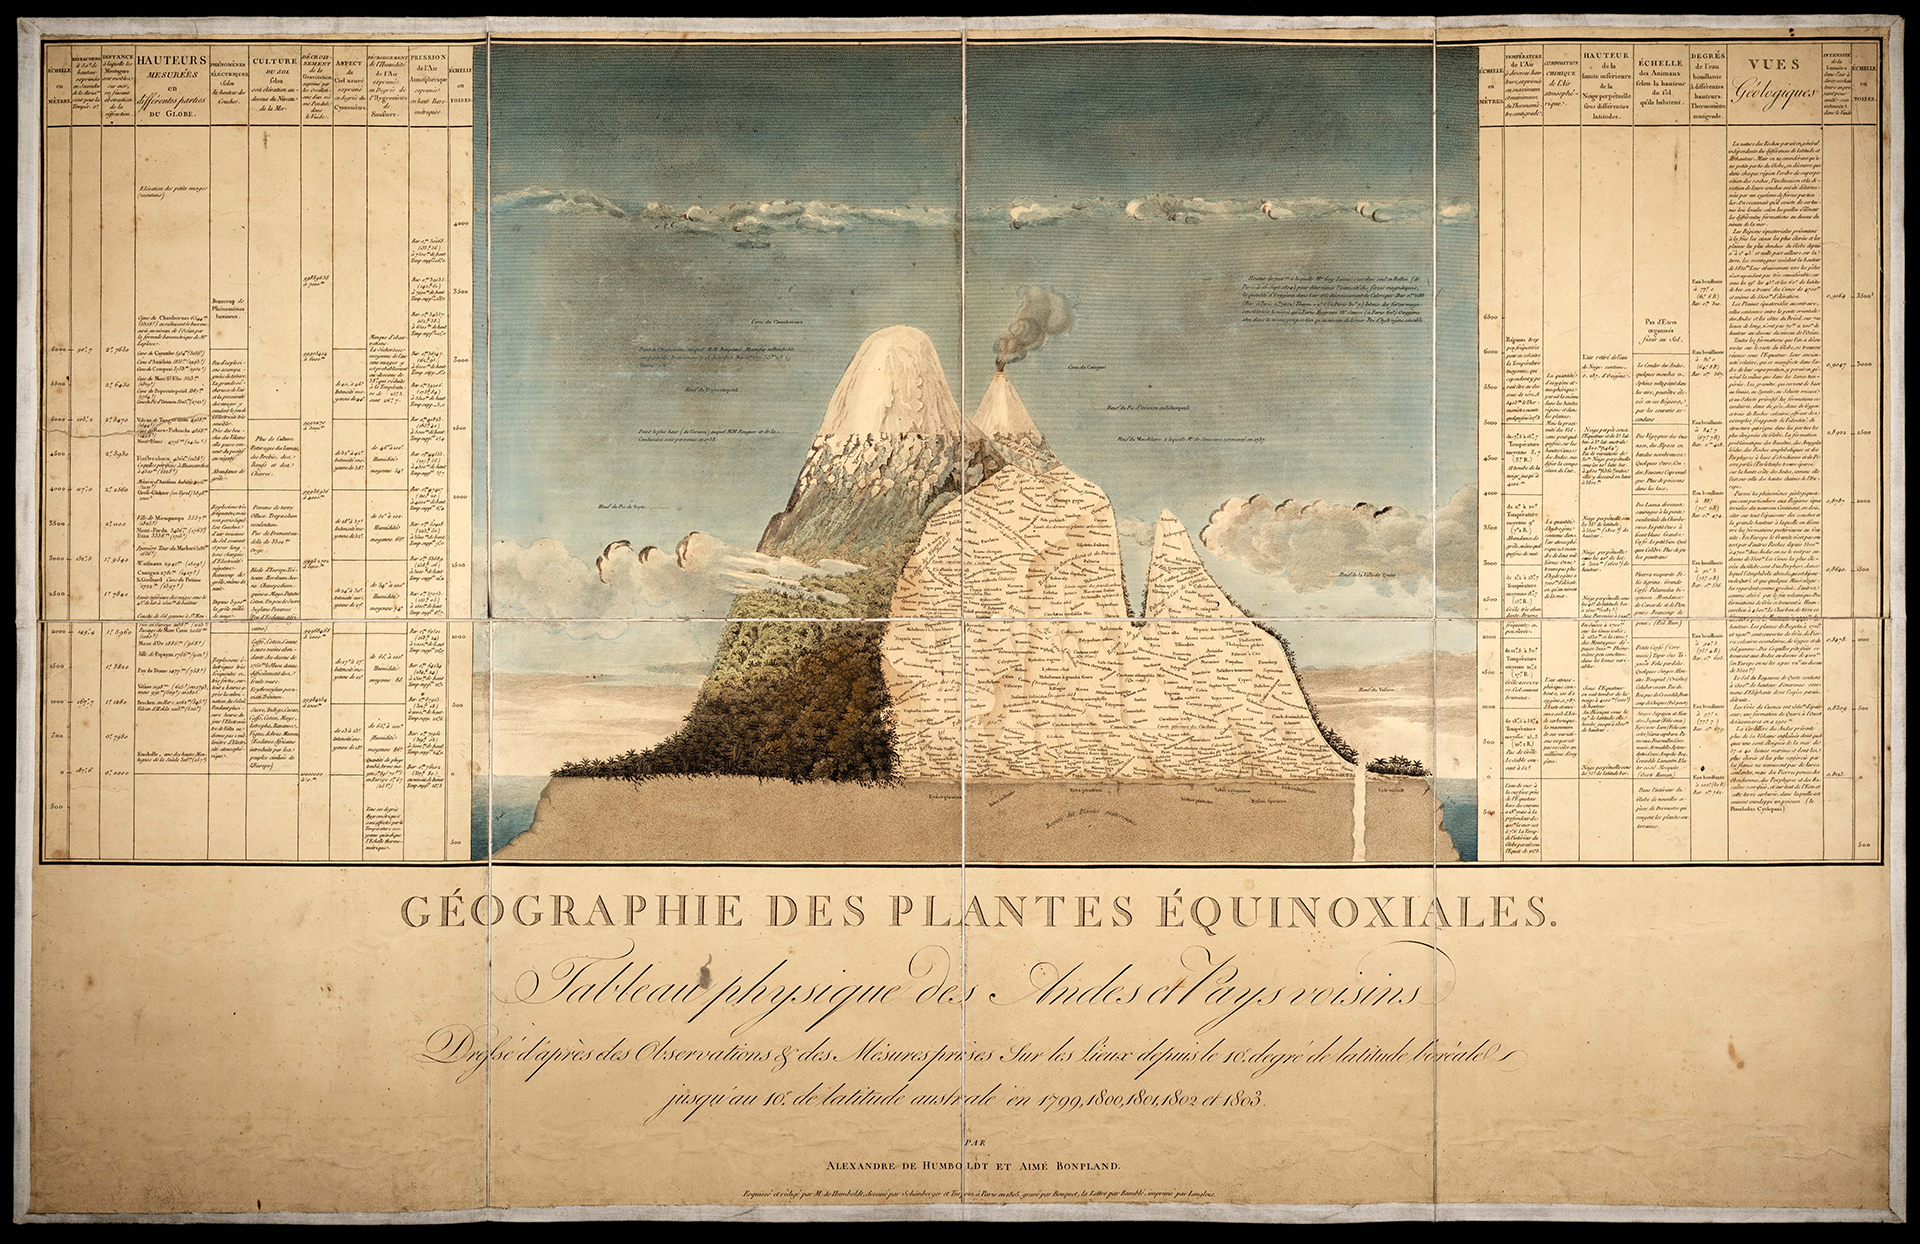
\includegraphics[width=0.80\textwidth]{figures/naturgemalde_humboldt.png}
  \caption{\textit{Naturgemälde} de Alexander von Humboldt (1805), representando a síntese zonal e altitudinal integrada entre clima, relevo e vegetação na Geografia Clássica. Fonte: Acervo histórico em domínio público.}
  \label{fig:humboldt_cap3}
\end{figure}

A partir da segunda metade do século XX, a especialização científica e os debates epistemológicos aprofundaram a cisão interna da disciplina. A \textbf{Geografia Teorético-Quantitativa} (1950--1970) modelou a natureza como sistema aberto de fluxos de matéria e energia por meio da Teoria Geral dos Sistemas e da estatística, o que fortaleceu estudos morfométricos de bacias hidrográficas e de climatologia dinâmica, mas introduziu risco de tecnicismo neutro ao abstrair conflitos políticos e desigualdades territoriais. Em resposta a esse formalismo, a \textbf{Geografia Crítica Clássica} (1970--1980) trouxe o materialismo histórico, o conflito de classes e a produção capitalista do espaço para o centro da análise, desnaturalizando a pobreza e a segregação urbana. Todavia, como observa Francisco Mendonça (2001), durante quase duas décadas parte expressiva da Geografia Humana crítica secundarizou a materialidade físico-ecológica (o chamado ``exílio da natureza''), enquanto setores da Geografia Física refugiaram-se em descrições estritamente naturalistas alheias à ação humana estruturante.

Somente a partir do final dos anos 1980 e desde a década de 1990, impulsionada pela crise ecológica global, pelas conferências ambientais (como a Rio-92) e pelo avanço das abordagens sistêmicas e socioambientais, a Geografia retomou o desafio de religar seus dois grandes ramos em bases metodológicas rigorosas. Situações concretas como a ocupação desigual de encostas e planícies urbanas (Figura~\ref{fig:segregacao_encosta_cap3}) ilustram por que a análise ambiental atual exige articular geomorfologia de vertentes e produção social do espaço mediante trabalho interdisciplinar, domínio de escalas e rigor de campo.

\begin{figure}[H]
  \centering
  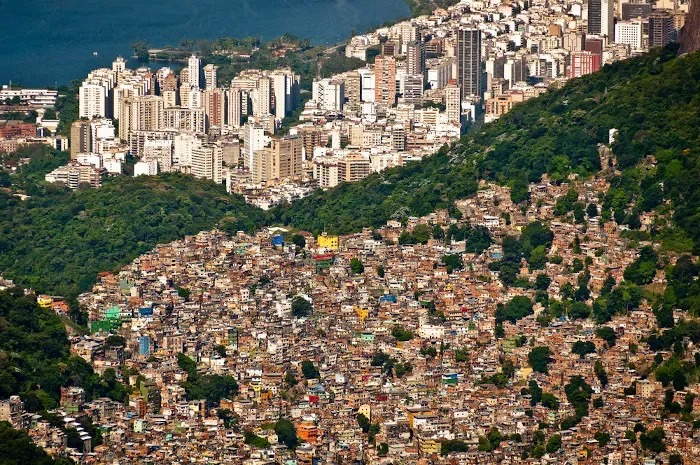
\includegraphics[width=0.78\textwidth]{figures/foto_segregacao_encosta_urbana.jpg}
  \caption{Ocupação desigual de encostas e planície urbana, evidenciando a necessidade de integrar geomorfologia de vertentes, drenagem e segregação socioespacial (Mendonça, 2001). Fonte: Acervo didático CHF662.}
  \label{fig:segregacao_encosta_cap3}
\end{figure}

\section{A Superação da Dicotomia e a Geografia Socioambiental (Mendonça, 2001)}

A divisão entre Geografia Física e Geografia Humana tornou-se um obstáculo operacional concreto para o geógrafo que atua em Análise Ambiental. Considere uma erosão em voçoroca que ameaça casas em um bairro periférico de Feira de Santana (BA) ou o assoreamento de um açude comunitário no Semiárido. Um diagnóstico restrito à erodibilidade do solo, à declividade da vertente e à intensidade das chuvas ignora a ausência de drenagem urbana, o loteamento irregular em Área de Preservação Permanente (APP) e a omissão do poder público. Inversamente, um diagnóstico limitado à especulação imobiliária e à segregação socioespacial deixa de medir declividade, textura do solo, vazão de pico e capacidade de infiltração, falhando ao dimensionar soluções para conter a voçoroca ou estabilizar o talude.

Diante dessa insuficiência bilateral, Francisco Mendonça (2001) sistematizou a proposta da \textbf{Geografia Socioambiental}. O autor demonstra que a palavra ``ambiente'' frequentemente era apropriada no Brasil por duas tradições incompletas, quais sejam a tradição naturalista, que a confundia com ecologia biológica sem seres humanos, e a tradição conservacionista pontual, desconectada dos conflitos territoriais. Na Geografia Socioambiental, o prefixo \textit{socio} constitui um posicionamento científico explícito, reafirmando que os problemas ambientais contemporâneos decorrem da interação indissociável entre a dinâmica dos elementos naturais (clima, relevo, água, solo e vegetação) e a organização social (modo de produção, técnica, legislação, desigualdade e cultura). Todo fenômeno ambiental envolve simultaneamente processos biofísicos e sociais, pois a degradação atinge desigualmente grupos situados no território e toda intervenção técnica sobre o meio físico resulta de escolhas econômicas e políticas. Ao preservar as especialidades técnicas da geomorfologia, da pedologia, da climatologia e da geografia urbana ou agrária, essa abordagem combate o isolamento compartimentado ao formular o problema ambiental, desde a origem, como uma questão híbrida de mútua determinação. O Exemplo 3.1 ilustra como essa reformulação opera diante de enchentes urbanas.

\begin{boxExemplo}{3.1 (Básico)}{Superando a Dicotomia Físico-Humana em Enchentes Urbanas}
\passoEnunciado{Durante a estação chuvosa, bairros situados na cabeceira do Rio Subaé, em Feira de Santana (BA), sofrem alagamentos recorrentes. Dois consultores emitiram pareceres conflitantes, com o Parecer 1 atribuindo o problema exclusivamente a chuvas convectivas intensas e relevo plano mal drenado, e o Parecer 2 sustentando que se trata apenas de segregação urbana e descaso político, sem considerar a hidrografia local. Reformule o diagnóstico sob a ótica da Geografia Socioambiental.}
\passoDados{Cabeceira urbana do Rio Subaé (Feira de Santana, BA); Parecer 1 focado exclusivamente em pluviosidade e topografia; Parecer 2 focado exclusivamente em segregação urbana e gestão municipal; referencial de Mendonça (2001).}
\passoPedido{Identificar o viés epistemológico presente em cada parecer e propor uma formulação integrada que supere a dicotomia.}
\passoMetodo{Análise epistemológica pela Geografia Socioambiental (Mendonça, 2001), verificando como processos físico-hidrológicos e decisões socioespaciais se codeterminam.}
\passoContas{%
\textbf{Passo 1, Diagnóstico do Parecer 1.} Reproduz o reducionismo naturalista (Geografia Física isolada). Ao atribuir o alagamento apenas à chuva e ao relevo plano, naturaliza um evento que foi amplificado pela impermeabilização do solo, pelo aterramento de nascentes e lagoas e pela ocupação de planícies de inundação.\\
\textbf{Passo 2, Diagnóstico do Parecer 2.} Reproduz o reducionismo sociologizante (Geografia Humana sem base material). Embora aponte corretamente a desigualdade urbana, ignora parâmetros físicos indispensáveis (capacidade de infiltração, cota de inundação e seção de escoamento), impedindo o dimensionamento de soluções drenantes.\\
\textbf{Passo 3, Reformulação socioambiental integrada.} Articula os dois eixos em uma cadeia causal única, onde a expansão urbana sem planejamento impermeabilizou áreas de recarga e estreitou canais naturais (processo social e territorial), o que reduziu a infiltração e elevou o escoamento superficial em eventos de chuva intensa sobre relevo de baixa declividade (dinâmica físico-hidrológica), atingindo prioritariamente famílias de menor renda assentadas nas áreas de várzea (desigualdade socioespacial).}
\passoResposta{Ambos os pareceres são dicotômicos (naturalista no Parecer 1 e sociologizante no Parecer 2). A leitura socioambiental integra a dinâmica hidrológica da cabeceira (infiltração, relevo plano e chuvas intensas) à produção desigual do espaço urbano (impermeabilização, aterramento de lagoas e vulnerabilidade habitacional).}
\passoVerificacao{A síntese faz sentido ambiental e técnico porque permite combinar ações estruturais (parques lineares, retenção de águas pluviais e desimpermeabilização) com ações territoriais e sociais (revisão do zoneamento urbano e regularização fundiária segura).}
\end{boxExemplo}

Aplicar a abordagem de Mendonça (2001) exige ir além da simples reunião de capítulos temáticos independentes, erro metodológico destacado a seguir.

\begin{boxErro}[Erro 1: Confundir Geografia Socioambiental com Soma Mecânica de Capítulos]
\textbf{Equívoco frequente:} acreditar que basta escrever uma seção de ``aspectos físicos'' (clima, relevo e solo) e outra seção separada de ``aspectos humanos'' (população e economia) para cumprir a abordagem socioambiental de Mendonça (2001).

\textbf{Por que está incorreto:} justapor partes desconexas reproduz a dicotomia clássico-positivista sob aparência integrada (multidisciplinaridade fragmentada).

\textbf{Como evitar:} explicite sempre as \textbf{relações causais e de retroalimentação} entre as dinâmicas naturais e sociais, mostrando como o manejo do solo intensifica a erosão e como essa erosão reduz a renda agrícola e agrava conflitos locais.
\end{boxErro}

\section{Distinção Rigorosa e Articulação: Espaço, Paisagem, Território e Ambiente}

Um dos erros mais frequentes em provas universitárias, relatórios de licenciamento e estudos orientados consiste em empregar \textit{espaço}, \textit{paisagem}, \textit{território} e \textit{ambiente} como palavras intercambiáveis para evitar repetições textuais. Em Análise Ambiental, cada uma dessas quatro categorias recorta um ângulo analítico específico da realidade geográfica e ativa instrumentos distintos de diagnóstico.

Como categoria matriz e mais abrangente da Geografia, o \textbf{espaço geográfico} representa, conforme a formulação clássica de Milton Santos, um conjunto indissociável, solidário e contraditório de sistemas de objetos (naturais e técnicos) e sistemas de ações (sociais, econômicas e normativas). Respondendo a como o espaço é produzido e reorganizado historicamente, essa categoria abrange, no Semiárido Baiano, a expansão da infraestrutura energética e viária que integra o sertão à rede elétrica nacional.

Em recorte imediato da experiência sensível, a \textbf{paisagem} corresponde à dimensão visível, material e simbólica do espaço geográfico em determinado momento, interrogando o que se vê, como a forma se estrutura e que sentido ela possui para os grupos locais. Resulta da acumulação desigual de tempos da natureza (geológico, geomorfológico e ecológico) e tempos sociais (formas de cultivo, estradas, cidades e represas). Na análise ambiental, permite ler marcas concretas de estabilidade ou degradação e expressa o vínculo cultural com o lugar, a exemplo do mosaico de caatinga arbustiva, afloramentos graníticos, pastagens e torres eólicas visíveis nas serras sertanejas.

Quando o foco recai sobre quem controla, regula, usa e disputa determinada área, mobiliza-se a categoria \textbf{território}, definida por relações de poder, apropriação, delimitação jurídica e gestão. Um município, uma bacia hidrográfica sob comitê de gestão, uma Unidade de Conservação, um assentamento rural ou a poligonal de um parque eólico constituem territórios. Sem essa categoria, o diagnóstico deixa de identificar quem decide, quem lucra, quem arca com os custos da degradação e quais normas incidem sobre o local, como ocorre na sobreposição entre contratos de arrendamento eólico, terras de fundo de pasto e limites de APP.

De modo complementar, o \textbf{ambiente} expressa o sistema relacional formado pelas interações entre fatores abióticos (clima, água, solo e relevo), bióticos (flora, fauna e microrganismos) e antrópicos (tecnologia, uso da terra, infraestrutura e organização social). Orientado pela pergunta de como os fluxos ecológicos e sociais se afetam mutuamente, esse conceito pressupõe um sistema de referência com o qual os fatores físicos, bióticos e sociais interagem, permitindo avaliar como a supressão vegetal em vertente altera o escoamento superficial, a perda de solo e a fauna associada no Semiárido. O Exemplo 3.2 exercita essa distinção a partir de registros de campo na Lagoa Grande, em Feira de Santana.

\begin{boxExemplo}{3.2 (Básico)}{Distinção Operacional entre Espaço, Paisagem, Território e Ambiente}
\passoEnunciado{Uma equipe de estudantes de CHF662 realiza trabalho de campo no entorno da Lagoa Grande, em Feira de Santana (BA), área que passou por obras de urbanização, requalificação paisagística e controle de drenagem. Em seus cadernos de campo, os alunos registraram quatro observações distintas e precisam classificá-las corretamente segundo as quatro categorias geográficas estudadas.}
\passoDados{Observação I registra que as margens exibem espelho d'água cercado por macrófitas, pista de caminhada, vegetação arbustiva e bairros residenciais, sendo reconhecidas pela população como área de lazer e memória hídrica da cidade. Observação II registra que a fiscalização municipal e a legislação estadual de APP delimitam faixas não edificáveis e regulam o uso comercial no entorno. Observação III registra que o aporte de esgoto clandestino elevou a carga de nutrientes na água, reduzindo o oxigênio dissolvido e alterando a biota aquática. Observação IV registra que a requalificação insere a lagoa na rede viária e na valorização imobiliária da malha urbana de Feira de Santana, reorganizando objetos técnicos e fluxos da cidade.}
\passoPedido{Associar cada observação à categoria geográfica predominante (espaço geográfico, paisagem, território ou ambiente) e justificar tecnicamente cada enquadramento.}
\passoMetodo{Aplicação dos núcleos analíticos e perguntas-chave definidos na Seção 3.3 deste capítulo.}
\passoContas{%
\textbf{Passo 1, Observação I.} Enfatiza a fisionomia visível (espelho d'água, vegetação, pista e bairros) e a percepção e memória afetiva da população, correspondendo à categoria \textbf{Paisagem}.\\
\textbf{Passo 2, Observação II.} Enfatiza normas jurídicas (APP), fiscalização estatal, delimitação de faixas e controle de uso, tratando de relações de poder e gestão e correspondendo à categoria \textbf{Território}.\\
\textbf{Passo 3, Observação III.} Descreve interações físico-químicas, bióticas e antrópicas (carga de nutrientes causando redução de oxigênio dissolvido e alteração da biota), correspondendo à categoria \textbf{Ambiente}.\\
\textbf{Passo 4, Observação IV.} Aborda a totalidade da produção urbana (integração de sistemas de objetos viários e imobiliários e sistemas de ações econômicas na cidade), correspondendo à categoria \textbf{Espaço Geográfico}.}
\passoResposta{I corresponde a Paisagem; II corresponde a Território; III corresponde a Ambiente; IV corresponde a Espaço Geográfico.}
\passoVerificacao{Cada categoria respondeu a uma pergunta diferente sobre o mesmo lugar (Lagoa Grande), comprovando que os quatro termos possuem núcleos analíticos próprios e se complementam na construção do diagnóstico.}
\end{boxExemplo}

Empregar essas categorias como meros sinônimos estilísticos compromete a precisão jurídica e técnica de laudos ambientais, como adverte o Erro 2.

\begin{boxErro}[Erro 2: Empregar Espaço, Paisagem, Território e Ambiente como Sinônimos]
\textbf{Equívoco frequente:} em textos acadêmicos e relatórios, o estudante escreve ``território'' em um parágrafo e ``paisagem'' ou ``ambiente'' no parágrafo seguinte apenas para evitar repetir a mesma palavra.

\textbf{Por que está incorreto:} cada categoria define um recorte teórico e operacional distinto. Falar em ``preservar a paisagem'' quando o conflito envolve disputa fundiária ou poder de gestão (território) enfraquece a precisão técnica do argumento.

\textbf{Como evitar:} antes de escolher o termo, verifique o foco da frase, utilizando \textit{território} para poder, gestão e norma, \textit{paisagem} para fisionomia, memória e percepção, \textit{ambiente} para interação físico-biótico-social e \textit{espaço geográfico} para a totalidade de objetos e ações.
\end{boxErro}

\section{O Esboço Metodológico da Paisagem e o Sistema Tripolar GTP (Bertrand, 2004)}

O geógrafo francês Georges Bertrand exerceu influência decisiva sobre a Análise Ambiental brasileira. Em seu texto clássico de 1968 (\textit{Paisagem e Geografia Física Global, esboço metodológico}), traduzido no Brasil em 1971 e republicado em 2004, Bertrand definiu a paisagem como o resultado da combinação dinâmica e instável de elementos físicos, biológicos e antrópicos que, reagindo dialeticamente uns sobre os outros, formam um conjunto único e indissociável em perpétua evolução. Naquela primeira formulação, Bertrand propôs uma taxonomia escalar centrada no conceito de \textbf{geossistema}, entendido como a interseção entre \textit{potencial ecológico} (geomorfologia, clima e hidrologia), \textit{exploração biológica} (vegetação, solo e fauna) e \textit{ação antrópica}.

Posteriormente, reconhecendo que o conceito de geossistema mantinha forte peso naturalista e demandava maior integração com as dimensões políticas, econômicas e simbólicas dos problemas ambientais contemporâneos, Georges Bertrand (em conjunto com Claude Bertrand, em textos difundidos no Brasil a partir de 2004) reformulou sua proposta no \textbf{Sistema Tripolar GTP (Geossistema, Território e Paisagem)}. Em conjunto com a tríade socioambiental de Mendonça (2001), que situa a Análise Ambiental Integrada na interseção entre Meio Físico, Meio Biótico e Sociedade \& Território (Figura~\ref{fig:triade-gtp}, Subfigura (a)), o modelo GTP estabelece três entradas metodológicas articuladas por setas bidirecionais (Figura~\ref{fig:triade-gtp}, Subfigura (b)).

\begin{figure}[htbp]
  \centering
  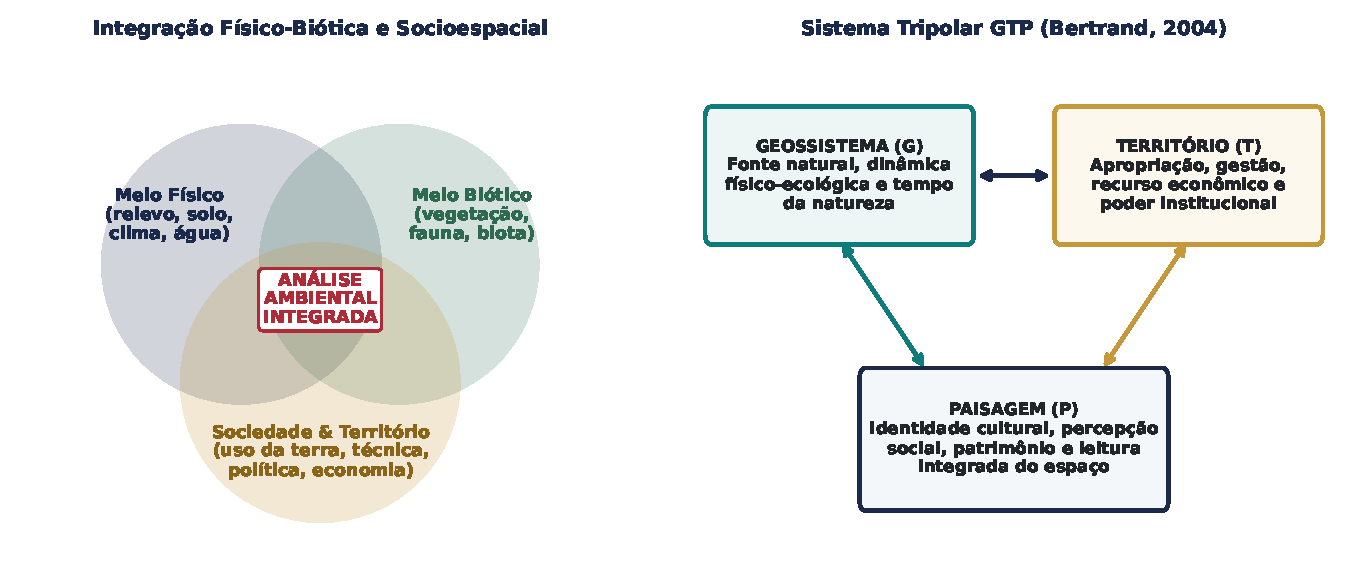
\includegraphics[width=0.94\textwidth]{figures/fig01_triade_socioambiental.pdf}
  \caption{Fundamentos integradores da Análise Ambiental na Geografia moderna: (a) interseção entre Meio Físico, Meio Biótico e Sociedade \& Território (Mendonça, 2001); (b) Sistema Tripolar GTP de Georges Bertrand (2004) com relações bidirecionais entre Geossistema (G), Território (T) e Paisagem (P). Fonte: Elaboração didática CHF662.}
  \label{fig:triade-gtp}
\end{figure}

Cada polo do Sistema GTP interroga o mesmo objeto socioambiental em uma temporalidade própria. O \textbf{Polo G, Geossistema} (a \textit{fonte} ou \textit{source}), analisa o funcionamento biofísico e ecológico do espaço e incorpora a antropização como força atuante nos fluxos de energia, água, sedimentos e nutrientes, operando principalmente no \textit{tempo da natureza}. O \textbf{Polo T, Território} (o \textit{recurso} ou \textit{ressource}), examina a dimensão socioeconômica, jurídica e política, tratando dos modos de apropriação, uso produtivo da terra, regulação legal, gestão de bacias e distribuição desigual de benefícios e danos no \textit{tempo social e institucional}. O \textbf{Polo P, Paisagem} (a \textit{ressurgência}, identidade e patrimônio, ou \textit{ressourcement}), investiga a dimensão cultural, simbólica, estética e perceptiva no \textit{tempo da memória e da cultura}.

Na prática de diagnósticos socioambientais, a fricção simultânea entre o uso territorial intensivo, a capacidade de suporte do meio físico e os conflitos culturais de apropriação exige articular os três polos com a hierarquia taxonômica das unidades inferiores propostas por Bertrand, variando da escala regional da \textit{Região Natural} ($100$ a $1.000\text{ km}$, cartografia $1:250.000$ ou menor) ao \textit{Geossistema} (alguns a dezenas de $\text{km}^2$, escala $1:50.000$), ao \textit{Geofácies} (centenas de $\text{m}^2$, escala $1:10.000$) e ao \textit{Geótopo} (dezenas de $\text{m}^2$, como uma voçoroca, em levantamento $1:2.000$), conforme organizado na Figura~\ref{fig:gtp_paisagem_taxonomia}. As setas bidirecionais entre G, T e P indicam que uma decisão territorial (como liberar loteamentos em cabeceiras) altera o funcionamento do geossistema (elevando o escoamento e os picos de cheia) e transforma a paisagem, assim como a mobilização cultural por uma paisagem patrimonial (P) pode induzir a criação de uma Unidade de Conservação (T) que estabiliza o balanço hídrico (G).

\begin{figure}[H]
  \centering
  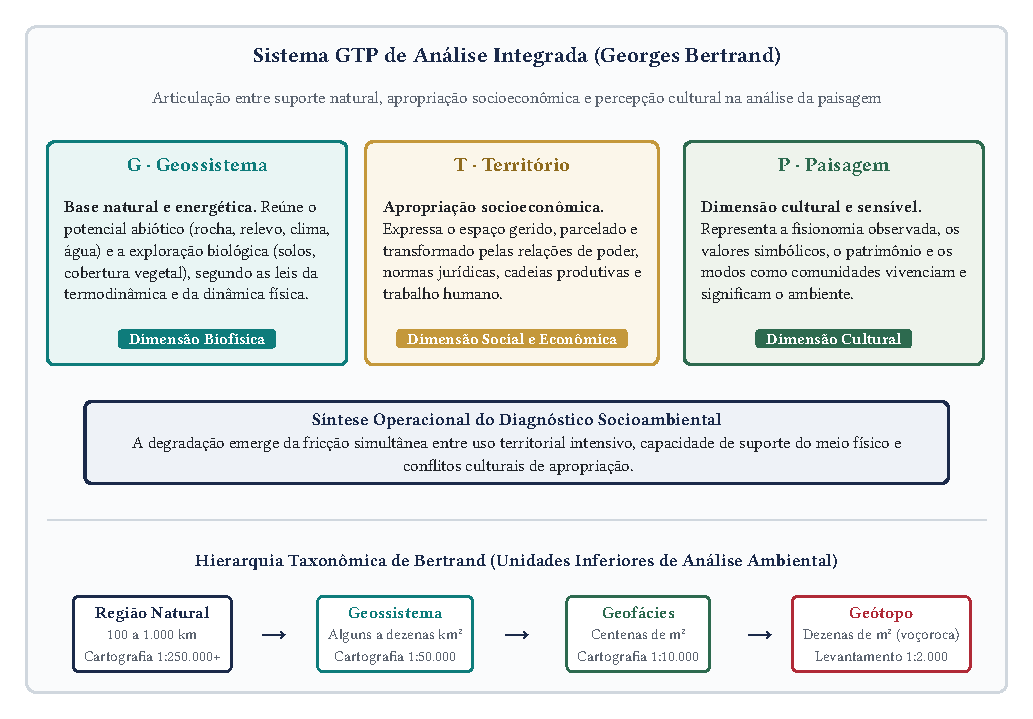
\includegraphics[width=0.94\textwidth]{figures/fig_cap03_gtp_paisagem.pdf}
  \caption{Articulação entre os três polos do Sistema GTP (Geossistema, Território e Paisagem) e a hierarquia taxonômica de Bertrand para as unidades inferiores de análise ambiental e suas escalas cartográficas de trabalho. Fonte: Elaboração didática CHF662.}
  \label{fig:gtp_paisagem_taxonomia}
\end{figure}

O Exemplo 3.3 aplica o Sistema Tripolar GTP e suas retroalimentações a um complexo eólico no Semiárido Baiano.

\begin{boxExemplo}{3.3 (Intermediário)}{Aplicação do Sistema Tripolar GTP em Parque Eólico no Semiárido}
\passoEnunciado{Na preparação para a atividade de campo de CHF662 no eixo energético do Semiárido Baiano (região de Canudos e Sertão), solicita-se estruturar um roteiro de análise integrada sobre a implantação de um complexo eólico em chapadas e tabuleiros de Caatinga, utilizando o Sistema Tripolar GTP de Georges Bertrand (2004).}
\passoDados{Elementos identificados em campo compreendem abertura de acessos e terraplanagem para bases de aerogeradores em solos arenosos e pedregosos de Caatinga com ravinamento incipiente nas bordas das plataformas (a); contratos de arrendamento de terras entre empresas energéticas e proprietários ou posseiros, além do licenciamento junto ao INEMA e disputas por áreas de pastoreio comunitário (b); e transformação visual das serras sertanejas pelas torres de grande porte, ruído aerodinâmico e ressignificação do lugar pelos moradores locais (c).}
\passoPedido{Enquadrar os elementos nos polos G, T e P e demonstrar duas retroalimentações (interações bidirecionais) entre os polos.}
\passoMetodo{Matriz tripolar GTP de Bertrand (2004), compreendendo Geossistema (fonte e biofísico), Território (recurso, gestão e poder) e Paisagem (identidade, percepção e patrimônio).}
\passoContas{%
\textbf{Passo 1, Enquadramento no Polo G (Geossistema).} Refere-se aos elementos (a), analisando a remoção da Caatinga, a exposição de solos frágeis ao impacto das chuvas concentradas do Semiárido, o escoamento concentrado nas estradas de serviço, a formação de ravinas nas bases das torres e os efeitos sobre a avifauna local.\\
\textbf{Passo 2, Enquadramento no Polo T (Território).} Refere-se aos elementos (b), analisando a governança energética, os contratos de arrendamento, as condicionantes do licenciamento ambiental (INEMA), a reorganização fundiária e os conflitos de acesso a áreas tradicionais de fundo de pasto.\\
\textbf{Passo 3, Enquadramento no Polo P (Paisagem).} Refere-se aos elementos (c), analisando a alteração da fisionomia das serras, a percepção sonora e visual do parque pelos moradores e o conflito entre o discurso da ``energia limpa'' e a memória territorial sertaneja.\\
\textbf{Passo 4, Interações bidirecionais.} Na interação $T \leftrightarrow G$, decisões contratuais e de traçado viário ($T$) determinam onde ocorrerá supressão vegetal e terraplanagem, desencadeando erosão em encostas ($G$), enquanto a erosão que desestabiliza estradas e taludes ($G$) impõe custos de manutenção e obrigações corretivas no licenciamento ($T$). Na interação $P \leftrightarrow T$, a percepção negativa de ruído e de descaracterização das serras ($P$) fortalece a mobilização comunitária por audiências públicas e revisão de distâncias mínimas das torres em relação às casas ($T$).}
\passoResposta{Polo G trata da dinâmica solo-água-vegetação-avifauna nas plataformas e acessos; Polo T trata de arrendamentos, licenciamento e conflitos fundiários; Polo P trata da reconfiguração visual e sonora e da identidade sertaneja. As conexões $T \leftrightarrow G$ e $P \leftrightarrow T$ evidenciam a indivisibilidade do sistema.}
\passoVerificacao{O roteiro cobre todas as dimensões exigidas na viagem de campo da Semana 11, evitando reduzir a energia eólica a um debate exclusivamente técnico-elétrico ou exclusivamente paisagístico.}
\end{boxExemplo}

Um equívoco frequente ao operar esse modelo consiste em supor que o Geossistema se restringe a ambientes sem presença humana, conforme destacado abaixo.

\begin{boxErro}[Erro 3: Entender o Polo Geossistema (G) como ``Natureza Intocada'']
\textbf{Equívoco frequente:} imaginar que, no Sistema GTP de Bertrand (2004), o Geossistema exclui qualquer ação humana e só existiria em florestas virgens ou parques sem moradores.

\textbf{Por que está incorreto:} desde 1968, e de forma ainda mais clara no modelo GTP, Bertrand inclui a \textbf{antropização} como componente interno da dinâmica geossistêmica. Uma bacia rural cultivada ou uma várzea urbana continuam operando como geossistemas profundamente modificados pela sociedade.

\textbf{Como evitar:} lembre que o polo G focaliza o \textit{funcionamento biofísico e ecológico} (incluindo os efeitos físicos da ação humana), enquanto os polos T e P tratam da gestão e poder e da identidade e percepção.
\end{boxErro}

Para auditar se um relatório ambiental integra os três polos de Bertrand (2004) de modo equilibrado entre o meio físico e a dimensão social, adota-se em CHF662 uma métrica didática de treinamento baseada na média harmônica das notas de cobertura técnica de cada polo ($g, t, p \in [0, 10]$). Diferentemente da média aritmética simples, a média harmônica penaliza fortemente o polo deficitário, refletindo o princípio sistêmico de que a integração é limitada pelo elo mais fraco. Esse recurso didático complementa o julgamento técnico sem substituir as evidências qualitativas e quantitativas que sustentam cada nota atribuída na rubrica de avaliação.

\begin{boxFormula}[Índice Didático de Equilíbrio Analítico GTP ($I_{\text{GTP}}$)]
\[
I_{\text{GTP}} = \frac{3\,g\,t\,p}{g\,t + g\,p + t\,p} \qquad (\text{para } g, t, p > 0; \quad I_{\text{GTP}} = 0 \text{ se } g = 0, \, t = 0 \text{ ou } p = 0)
\]
Nas aplicações de CHF662, $g$, $t$ e $p$ representam as notas de cobertura técnica ($0$ a $10$) atribuídas aos polos Geossistema, Território e Paisagem segundo rubrica explícita. Valores de $I_{\text{GTP}} \ge 7{,}0$ indicam diagnóstico bem integrado nos três polos; o intervalo $4{,}0 \le I_{\text{GTP}} < 7{,}0$ indica integração parcial com polo subdesenvolvido; e $I_{\text{GTP}} < 4{,}0$ caracteriza diagnóstico fragmentado ou dicotômico.
\end{boxFormula}

O Exemplo 3.4 demonstra numericamente por que relatórios com a mesma média aritmética podem exibir níveis opostos de equilíbrio socioambiental quando avaliados pelo $I_{\text{GTP}}$.

\begin{boxExemplo}{3.4 (Intermediário)}{Auditoria Quantitativa de Relatórios Ambientais com o Índice $I_{\text{GTP}}$}
\passoEnunciado{Para subsidiar o plano de gestão de uma microbacia no Vale do Paraguaçu (BA), um órgão público avaliou dois diagnósticos preliminares elaborados por consultorias diferentes. A comissão avaliadora atribuiu notas de $0$ a $10$ para a consistência técnica em cada polo do sistema GTP. Verifique numericamente qual diagnóstico apresenta real integração socioambiental.}
\passoDados{Diagnóstico X com Geossistema $g_X = 10{,}0$, Território $t_X = 1{,}0$ e Paisagem $p_X = 1{,}0$. Diagnóstico Y com Geossistema $g_Y = 4{,}0$, Território $t_Y = 4{,}0$ e Paisagem $p_Y = 4{,}0$. Critério de referência $I_{\text{GTP}} = \frac{3\,g\,t\,p}{g\,t + g\,p + t\,p}$.}
\passoPedido{Calcular a média aritmética ($\text{MA}$) e o índice $I_{\text{GTP}}$ de ambos os diagnósticos e interpretar o significado metodológico da diferença encontrada.}
\passoMetodo{Cálculo passo a passo de $\text{MA}$ e $I_{\text{GTP}}$ conforme o quadro de fórmulas da Etapa 3.}
\passoContas{%
\textbf{Passo 1, Médias aritméticas.}
\[
\text{MA}_X = \frac{10{,}0 + 1{,}0 + 1{,}0}{3} = \frac{12{,}0}{3} = 4{,}00 \qquad\text{e}\qquad \text{MA}_Y = \frac{4{,}0 + 4{,}0 + 4{,}0}{3} = \frac{12{,}0}{3} = 4{,}00.
\]
Pela média aritmética simples, os dois relatórios pareceriam empatados.\\
\textbf{Passo 2, Cálculo de $I_{\text{GTP}}$ para o Diagnóstico X.} O numerador resulta em $3 \times 10{,}0 \times 1{,}0 \times 1{,}0 = 30{,}0$, e o denominador soma $(10{,}0 \times 1{,}0) + (10{,}0 \times 1{,}0) + (1{,}0 \times 1{,}0) = 21{,}0$, resultando em $I_{\text{GTP}, X} = \frac{30{,}0}{21{,}0} = \frac{10}{7} \approx 1{,}43$ (diagnóstico fragmentado e dicotômico).\\
\textbf{Passo 3, Cálculo de $I_{\text{GTP}}$ para o Diagnóstico Y.} O numerador alcança $3 \times 4{,}0 \times 4{,}0 \times 4{,}0 = 192{,}0$, e o denominador soma $(4{,}0 \times 4{,}0) + (4{,}0 \times 4{,}0) + (4{,}0 \times 4{,}0) = 48{,}0$, resultando em $I_{\text{GTP}, Y} = \frac{192{,}0}{48{,}0} = 4{,}00$ (integração parcial equilibrada).\\
\textbf{Passo 4, Comparação percentual.} O Diagnóstico Y obtém $I_{\text{GTP}}$ superior ao de X em $\frac{4{,}00 - 1{,}43}{1{,}43} \times 100\% \approx 180\%$, apesar da mesma soma de notas ($12{,}0$).}
\passoResposta{$\text{MA}_X = \text{MA}_Y = 4{,}00$; contudo, $I_{\text{GTP}, X} \approx 1{,}43$ (fragmentado) e $I_{\text{GTP}, Y} = 4{,}00$ (integração parcial equilibrada). O Diagnóstico Y mostra maior coerência com a abordagem socioambiental, embora ambos precisem ser aprimorados para atingir o patamar integrado ($\ge 7{,}0$).}
\passoVerificacao{O resultado respeita a desigualdade entre médias (a média harmônica é sempre menor ou igual à média aritmética, igualando-se apenas quando $g = t = p$) e a lógica ambiental, pois excelência isolada em mapeamento físico deixa sem resposta os conflitos territoriais e a percepção social.}
\end{boxExemplo}

\section{Interdisciplinaridade e Análise Ambiental Integrada}

Nenhuma disciplina isolada domina todos os métodos exigidos por um diagnóstico ambiental de alta complexidade. Entretanto, reunir diversos profissionais em uma mesma equipe raramente garante uma análise integrada, razão pela qual a epistemologia ambiental distingue três níveis de cooperação entre saberes. Na \textbf{multidisciplinaridade} (justaposição), especialistas como geólogo, biólogo, engenheiro, sociólogo e geógrafo elaboram capítulos separados sobre a mesma área, sem formular perguntas comuns nem cruzar variáveis, produzindo o ``relatório em gavetas'', no qual o capítulo de solos permanece isolado do de uso da terra e do de saúde pública. Na \textbf{interdisciplinaridade} (integração metodológica), diferentes disciplinas definem conjuntamente o problema ambiental, compatibilizam escalas espaciais e temporais, trocam dados e constroem sínteses integradas, como mapas de fragilidade socioambiental, matrizes de impacto cruzado e zoneamentos participativos. Na \textbf{transdisciplinaridade} (diálogo com saberes locais), além de integrar disciplinas científicas, o estudo incorpora o conhecimento empírico e territorial das comunidades (agricultores familiares, pescadores, comunidades de fundo de pasto e quilombolas), indispensável para compreender o regime histórico de riachos intermitentes, manchas de solo fértil e usos tradicionais da biota. Nesse arranjo, pela formação voltada à espacialidade, à cartografia temática, às escalas e à interface natureza-sociedade, o geógrafo atua como um \textit{articulador espacial}, capaz de traduzir dados setoriais em uma leitura territorial integrada e propositiva.

% ============================================================================
% ETAPA 4 - SÍNTESE AVANÇADA E ESTUDO DE CASO INTEGRADOR
% ============================================================================
\etapa{4}{Síntese Avançada: Desenho de Projeto Interdisciplinar em Microbacia}

A passagem de diagnósticos fragmentados para projetos interdisciplinares e transdisciplinares exige compatibilizar escalas cartográficas, definir uma unidade espacial comum e formular perguntas articuladoras que conectem processos físicos, gestão territorial e experiência comunitária. O Exemplo 3.5 demonstra como reestruturar um termo de referência originalmente multidisciplinar em uma microbacia periurbana baiana.

\begin{boxExemplo}{3.5 (Avançado)}{Desenho de Projeto Interdisciplinar em Microbacia Periurbana}
\passoEnunciado{A prefeitura de um município da Região Metropolitana de Feira de Santana contratou um estudo ambiental para uma microbacia afluente do Rio Jacuípe que enfrenta desmatamento de mata ciliar, retirada irregular de areia e expansão de chácaras sem esgotamento sanitário. A proposta inicial da empresa previa cinco relatórios isolados (Geologia, Botânica, Hidrologia, Economia e Sociologia) entregues em anexos separados, em escalas cartográficas diferentes ($1:100.000$ na Geologia e $1:5.000$ no cadastro urbano). Reestruture a proposta para garantir interdisciplinaridade efetiva.}
\passoDados{Microbacia periurbana afluente do Rio Jacuípe (BA); problemas de supressão ripária, mineração irregular de areia e loteamento sem saneamento; proposta inicial com 5 anexos independentes em escalas incompatíveis ($1:100.000$ e $1:5.000$).}
\passoPedido{Diagnosticar a falha metodológica da proposta original e propor um protocolo interdisciplinar e transdisciplinar de trabalho.}
\passoMetodo{Distinção entre multidisciplinaridade, interdisciplinaridade e transdisciplinaridade articulada ao papel integrador do geógrafo e à compatibilização de escalas.}
\passoContas{%
\textbf{Passo 1, Diagnóstico da falha.} A proposta original caracteriza \textbf{multidisciplinaridade justaposta}. Além da ausência de problema comum, a incompatibilidade escalar impede o cruzamento espacial, pois uma base geológica $1:100.000$ carece de resolução para localizar processos erosivos de margem e relacioná-los aos lotes em escala $1:5.000$.\\
\textbf{Passo 2, Recorte espacial e escala comum.} Adotar a \textbf{microbacia hidrográfica} como unidade física de integração, harmonizando todas as camadas temáticas (solos, declividade, cobertura vegetal, uso da terra, pontos de lançamento de efluentes e cavas de areia) na escala operacional de detalhe ($1:10.000$ ou $1:5.000$).\\
\textbf{Passo 3, Pergunta interdisciplinar unificadora.} Substituir os cinco inventários soltos por uma questão articuladora voltada a investigar como a expansão de chácaras e a extração de areia alteram a conectividade hidrossedimentológica, a qualidade da água e os conflitos territoriais na microbacia.\\
\textbf{Passo 4, Produtos integrados e transdisciplinaridade.} Gerar um mapa-síntese socioambiental (cruzando polos G, T e P) e realizar oficinas participativas com moradores e pequenos produtores para incorporar o histórico local de cheias, nascentes extintas e usos tradicionais da água (dimensão transdisciplinar).}
\passoResposta{A proposta original é meramente multidisciplinar e escalarmente incompatível. A reestruturação exige unidade espacial comum (microbacia em escala de detalhe $1:5.000$ a $1:10.000$), pergunta-problema compartilhada, matriz integradora GTP e oficinas participativas (transdisciplinaridade).}
\passoVerificacao{A solução assegura que os dados físicos (erosão e qualidade hídrica) orientem diretamente o ordenamento territorial e a fiscalização ambiental, evitando relatórios desconexos que permanecem sem aplicação prática.}
\end{boxExemplo}

% ============================================================================
% ETAPA 5 - ARMADILHA CONCEITUAL E MATERIAIS AUDIOVISUAIS DE APOIO
% ============================================================================
\etapa{5}{Armadilha Conceitual e Materiais Audiovisuais de Apoio}

Mesmo quando o diagnóstico ambiental equilibra bem os dados físicos do geossistema e as normas do território, é frequente negligenciar o polo Paisagem por considerá-lo subjetivo ou secundário, erro que compromete a aceitação social e a eficácia das intervenções.

\begin{boxErro}[Erro 4: Tratar a Paisagem (P) como Aspecto Meramente Decorativo ou Estético]
\textbf{Equívoco frequente:} desvalorizar o polo Paisagem do sistema GTP em diagnósticos ambientais, considerando-o ``subjetivo demais'' frente aos dados numéricos de solo e água.

\textbf{Por que está incorreto:} a paisagem expressa vínculos de pertencimento, memória coletiva e leitura histórica do espaço. Projetos de intervenção (como barragens, parques eólicos ou recuperação de lagoas urbanas) frequentemente fracassam ou geram forte resistência social quando ignoram o valor identitário e patrimonial que as comunidades atribuem à paisagem.

\textbf{Como evitar:} integre levantamentos de percepção ambiental, história oral e patrimônio paisagístico ao diagnóstico físico e territorial.
\end{boxErro}

Para ampliar a compreensão sobre a síntese integrada da paisagem e os grandes domínios morfoclimáticos na Geografia brasileira, assista à videoaula recomendada na página da disciplina, intitulada \textit{Domínios Morfoclimáticos do Brasil (Aziz Ab'Sáber)} (\url{https://www.youtube.com/watch?v=M9AaD1DZnnQ}), que apresenta a articulação entre relevo, clima, solos e cobertura vegetal na leitura espacial brasileira.

% ============================================================================
% ETAPA 6 - EXERCÍCIOS DE FIXAÇÃO (15 EXERCÍCIOS EM 3 NÍVEIS)
% ============================================================================
\etapa{6}{Exercícios de Fixação}

\subsection*{Nível Básico (Exercícios 1 a 5)}

\begin{enumerate}[leftmargin=1.8em, itemsep=4pt]
  \item Explique, com suas próprias palavras, qual é a principal diferença entre a visão da relação sociedade-natureza no \textbf{determinismo ambiental} e no \textbf{possibilismo}.
  \espacoResolucao[2.0cm]

  \item Por que a Geografia Crítica das décadas de 1970 e 1980, apesar de seus avanços na compreensão da produção social do espaço, acabou reforçando indiretamente a dicotomia entre Geografia Física e Geografia Humana?
  \espacoResolucao[2.0cm]

  \item Segundo Mendonça (2001), por que a expressão \textbf{Geografia Socioambiental} utiliza o prefixo ``socio''? Isso representa uma redundância conceitual? Justifique.
  \espacoResolucao[2.0cm]

  \item Indique os três polos do \textbf{Sistema Tripolar GTP} proposto por Georges Bertrand (2004), associando cada polo ao seu papel analítico principal (\textit{fonte}, \textit{recurso} ou \textit{identidade e patrimônio}).
  \espacoResolucao[2.0cm]

  \item Diferencie \textbf{multidisciplinaridade} de \textbf{interdisciplinaridade} na elaboração de um diagnóstico ambiental de bacia hidrográfica.
  \espacoResolucao[2.0cm]
\end{enumerate}

\subsection*{Nível Intermediário (Exercícios 6 a 10)}

\begin{enumerate}[leftmargin=1.8em, itemsep=4pt, resume]
  \item Observe a Figura~\ref{fig:triade-gtp} (Subfigura (b)). Por que as setas que conectam Geossistema (G), Território (T) e Paisagem (P) são \textbf{bidirecionais} ($\leftrightarrow$), diferenciando-se de setas de sentido único ($\rightarrow$)? Dê um exemplo concreto no Semiárido baiano.
  \espacoResolucao[2.3cm]

  \item Em um município do Recôncavo Baiano, a expansão de loteamentos sobre áreas de manguezal provocou supressão vegetal, assoreamento de canais de maré, disputa judicial com marisqueiras e perda de referência cultural da comunidade pesqueira. Classifique esses quatro fenômenos segundo as categorias \textbf{ambiente}, \textbf{território} e \textbf{paisagem}, indicando como eles se articulam no \textbf{espaço geográfico}.
  \espacoResolucao[2.5cm]

  \item Dois grupos de estudantes apresentaram propostas de Diagnóstico Ambiental para uma microbacia de Feira de Santana (BA) e receberam as seguintes notas nos polos GTP:
  \begin{itemize}[leftmargin=1.5em, itemsep=1pt]
    \item \textbf{Grupo 1,} $g = 10{,}0$; $t = 2{,}0$; $p = 2{,}0$.
    \item \textbf{Grupo 2,} $g = 6{,}0$; $t = 6{,}0$; $p = 6{,}0$.
  \end{itemize}
  Calcule a média aritmética ($\text{MA}$) e o índice de equilíbrio $I_{\text{GTP}}$ de cada grupo, passo a passo, e classifique o nível de integração de ambos os trabalhos.
  \espacoResolucao[2.8cm]

  \item Um parecer técnico sobre desertificação no norte da Bahia descreve detalhadamente o déficit hídrico climático e o sobrepastejo caprino, mas omite completamente a estrutura fundiária, a ausência de assistência técnica rural e o modo como os sertanejos percebem o ressecamento das nascentes. Analise criticamente esse parecer à luz do Sistema GTP.
  \espacoResolucao[2.3cm]

  \item Explique como a \textbf{transdisciplinaridade} pode enriquecer um diagnóstico ambiental conduzido por geógrafos em comunidades rurais de fundo de pasto no Semiárido baiano, citando dois tipos de informações locais que raramente constam em bases cartográficas oficiais.
  \espacoResolucao[2.3cm]
\end{enumerate}

\subsection*{Nível Aplicado: Questões Objetivas (Exercícios 11 a 15)}

\begin{enumerate}[leftmargin=1.8em, itemsep=5pt, resume]
  \item Em relação à evolução das abordagens ambientais no pensamento geográfico moderno, assinale a alternativa correta:
  \begin{alternativas}
    \item A Geografia Clássica do século XIX recusava qualquer estudo sobre clima, relevo ou vegetação, concentrando-se apenas na economia urbana.
    \item O determinismo ambiental defendia que a técnica humana supera integralmente os limites ecológicos de qualquer região.
    \item A Geografia Socioambiental (Mendonça, 2001) propõe superar a separação entre Geografia Física e Geografia Humana integrando processos naturais e dinâmicas sociais.
    \item A Geografia Teorético-Quantitativa eliminou o uso de modelos sistêmicos por considerá-los incompatíveis com a análise ambiental.
    \item A Geografia Crítica dos anos 1970 priorizou o estudo da pedogênese e da geomorfologia de vertentes como eixo central de suas pesquisas.
  \end{alternativas}
  \espacoResolucao[1.2cm]

  \item No planejamento de uma Unidade de Conservação na Chapada Diamantina (BA), o analista precisa examinar as normas de uso do solo, o zoneamento do plano de manejo e os conflitos de competência entre órgãos municipais, estaduais e associações comunitárias. A categoria geográfica que expressa diretamente essa dimensão de poder e gestão é:
  \begin{alternativas}
    \item Geótopo.
    \item Território.
    \item Potencial ecológico.
    \item Bioma.
    \item Clímax edáfico.
  \end{alternativas}
  \espacoResolucao[1.2cm]

  \item No Sistema Tripolar GTP de Georges Bertrand (2004), a correspondência correta entre os polos e seus respectivos focos analíticos é:
  \begin{alternativas}
    \item Geossistema = identidade cultural; Território = fluxos hidrológicos; Paisagem = normas jurídicas.
    \item Geossistema = recurso econômico; Território = tempo geológico; Paisagem = apenas estética de cartões-postais.
    \item Geossistema = natureza intocada sem ação humana; Território = clima regional; Paisagem = bacia hidrográfica.
    \item Geossistema = funcionamento biofísico e ecológico (fonte); Território = apropriação, gestão e poder (recurso); Paisagem = percepção, identidade e patrimônio (ressurgência).
    \item Geossistema = modelo matemático urbano; Território = vegetação nativa; Paisagem = levantamento topográfico sem observador.
  \end{alternativas}
  \espacoResolucao[1.2cm]

  \item Um Estudo de Impacto Ambiental (EIA) reúne capítulos elaborados isoladamente por um geólogo, um biólogo e um sociólogo, sem cruzamento cartográfico, sem padronização de escala e sem discussão conjunta das causas dos impactos. Epistemologicamente, esse estudo caracteriza-se como:
  \begin{alternativas}
    \item Transdisciplinar, pois envolve especialistas de diferentes áreas técnicas.
    \item Interdisciplinar, uma vez que contém tanto dados naturais quanto sociais no mesmo volume.
    \item Multidisciplinar justaposto, pois soma descrições setoriais sem integração metodológica real.
    \item Sistêmico tripolar, por apresentar exatamente três profissionais na equipe técnica.
    \item Possibilista integrado, por respeitar a autonomia absoluta de cada disciplina.
  \end{alternativas}
  \espacoResolucao[1.2cm]

  \item Um relatório de diagnóstico ambiental obteve notas $g = 8{,}0$ em Geossistema, $t = 8{,}0$ em Território e $p = 0{,}0$ em Paisagem (ausência total de análise paisagística e perceptiva). Aplicando o critério didático do índice $I_{\text{GTP}}$, conclui-se que:
  \begin{alternativas}
    \item O relatório alcança integração plena, pois a média aritmética dos dois polos preenchidos é $8{,}0$.
    \item $I_{\text{GTP}} = 0{,}0$, evidenciando ruptura da integração tripolar pela supressão completa do polo Paisagem.
    \item $I_{\text{GTP}} = 5{,}33$, classificando o relatório como parcialmente integrado.
    \item A ausência do polo Paisagem é irrelevante em diagnósticos ambientais, pois o polo P interfere pouco na gestão territorial.
    \item O relatório deve ser considerado de viés exclusivamente sociologizante.
  \end{alternativas}
  \espacoResolucao[1.2cm]
\end{enumerate}

% ============================================================================
% ETAPA 7 - QUESTÕES ESTILO ENADE E CONCURSOS AMBIENTAIS
% ============================================================================
\etapa{7}{Questões no Estilo ENADE e Concursos Ambientais}

\begin{boxDica}[Estratégia para o Estudo Orientado 2 (EO2) e para a Avaliação Teórica]
No \textbf{EO2} (Semana 3, baseado em Mendonça, 2001, e Bertrand, 2004) e na \textbf{Prova Teórica} (Semana 10), as questões dissertativas e objetivas costumam cobrar três habilidades integradas:
\begin{enumerate}[leftmargin=1.5em, itemsep=1.5pt]
  \item Demonstrar por que a análise ambiental supera tanto a Geografia Física isolada quanto a Geografia Humana desconectada da base biofísica.
  \item Aplicar corretamente as categorias \textit{espaço, paisagem, território e ambiente} a um caso concreto, evitando definições decoradas sem exemplo.
  \item Articular os três polos do \textbf{Sistema GTP} destacando as interações entre o tempo da natureza (G), o tempo da gestão e economia (T) e o tempo da cultura e memória (P).
\end{enumerate}
\end{boxDica}

\begin{enumerate}[leftmargin=1.8em, itemsep=5pt, start=16]
  \item \textbf{(Questão autoral, estilo ENADE / Geografia)} A implantação de grandes projetos de irrigação no Vale do São Francisco reorganizou o uso da água, substituiu extensas áreas de Caatinga por monocultivos de fruticultura, redefiniu relações fundiárias e alterou profundamente o modo como populações ribeirinhas vivenciam e representam o rio. Analisando essa transformação à luz da Geografia Socioambiental (Mendonça, 2001) e do Sistema GTP (Bertrand, 2004), avalie as afirmações a seguir:
  \begin{enumerate}[label=\Roman*., leftmargin=2.0em, itemsep=2pt]
    \item O polo Geossistema (G) permite investigar exclusivamente a vazão natural anterior à construção de barragens, devendo excluir os efeitos da irrigação sobre a salinização dos solos.
    \item O polo Território (T) evidencia a apropriação diferencial dos recursos hídricos, o papel das políticas públicas de irrigação e os conflitos entre grandes empreendimentos e agricultores familiares.
    \item O polo Paisagem (P) capta a reconfiguração fisionômica das margens e a transformação simbólica e identitária na relação das comunidades ribeirinhas com o rio.
    \item A articulação entre G, T e P supera a dicotomia clássico-positivista ao demonstrar que impactos hidrológicos e conflitos fundiários pertencem à mesma totalidade socioambiental.
  \end{enumerate}
  É correto apenas o que se afirma em:
  \begin{alternativas}
    \item I e II.
    \item I e III.
    \item II e IV.
    \item II, III e IV.
    \item I, II, III e IV.
  \end{alternativas}
  \espacoResolucao[1.3cm]

  \item \textbf{(Questão autoral, estilo Concurso Analista Ambiental / INEMA-IBAMA)} Em uma audiência pública para licenciamento de rodovia estadual que atravessa serras e comunidades tradicionais no interior da Bahia, a equipe consultora apresentou um relatório contendo mapas detalhados de litologia, declividade e remanescentes florestais, mas declarou que ``os conflitos fundiários e o valor cultural atribuído às serras pelas comunidades locais fogem ao escopo ambiental por serem temas estritamente sociológicos''. À luz dos fundamentos da Análise Ambiental na Geografia moderna, essa justificativa é:
  \begin{alternativas}
    \item Correta, pois a análise ambiental restringe-se aos meios físico e biótico, deixando questões territoriais para o Poder Judiciário.
    \item Correta, visto que o conceito de geossistema exclui variáveis culturais e institucionais de qualquer estudo de impacto.
    \item Incorreta, pois reproduz a dicotomia natureza-sociedade e desconsidera que território e paisagem são dimensões constitutivas da análise ambiental integrada.
    \item Incorreta apenas quanto aos conflitos fundiários, sendo correta quanto à exclusão do valor cultural das serras, que carece de relevância geográfica.
    \item Parcialmente correta, pois a interdisciplinaridade exige que os temas sociais sejam analisados somente após a emissão da licença de operação.
  \end{alternativas}
  \espacoResolucao[1.3cm]

  \item \textbf{(Questão autoral, estilo Concurso Geógrafo / Planejamento Territorial)} Assinale a alternativa que estabelece corretamente a relação entre \textbf{escala}, \textbf{interdisciplinaridade} e \textbf{categorias geográficas} na condução de um diagnóstico ambiental aplicado em microbacias hidrográficas:
  \begin{alternativas}
    \item A justaposição de mapas em escalas incompatíveis ($1:250.000$ e $1:2.000$) é desejável porque amplia a diversidade de fontes no relatório multidisciplinar.
    \item O geógrafo substitui integralmente biólogos, engenheiros e juristas na análise ambiental, dispensando a cooperação interdisciplinar.
    \item A distinção entre espaço, paisagem, território e ambiente é irrelevante na prática técnica, servindo apenas para debates filosóficos sem repercussão cartográfica.
    \item A análise ambiental integrada requer compatibilização de escalas espaciais e temporais, formulação interdisciplinar do problema e articulação das dinâmicas biofísicas (G) com a gestão territorial (T) e a leitura paisagística (P).
    \item A transdisciplinaridade consiste em substituir medições de campo e dados hidrológicos exclusivamente por relatos informais de moradores locais.
  \end{alternativas}
  \espacoResolucao[1.3cm]
\end{enumerate}

% ============================================================================
% ETAPA 8 - GABARITO INTEGRALMENTE COMENTADO (EM PÁGINA SEPARADA)
% ============================================================================
\clearpage
\etapa{8}{Gabarito Integralmente Comentado (Exercícios 1 a 18)}

\begin{boxGabarito}[Resolução: Nível Básico (Exercícios 1 a 5)]
\begin{enumerate}[leftmargin=1.8em, itemsep=4pt]
  \item \textbf{Determinismo e Possibilismo.} No \textit{determinismo ambiental} (associado a Ratzel e leituras deterministas posteriores), as condições naturais (clima, relevo e solo) determinam diretamente a organização e o desenvolvimento das sociedades. No \textit{possibilismo} (Vidal de La Blache), a natureza oferece possibilidades e condicionantes, cabendo à sociedade escolher, adaptar-se e transformar o meio por intermédio da técnica, da cultura e do \textit{gênero de vida}.
  \item \textbf{Geografia Crítica e dicotomia.} Ao reagir ao formalismo quantitativo e priorizar o materialismo histórico e as relações sociais de produção, parte expressiva da Geografia Humana crítica dos anos 1970--1980 afastou-se do estudo dos processos naturais (relevo, solos, clima e hidrologia). Em paralelo, setores da Geografia Física mantiveram-se restritos a análises naturalistas, consolidando duas comunidades científicas com pouco diálogo.
  \item \textbf{Prefixo ``socio'' em Mendonça (2001).} A escolha evita qualquer redundância. Ela marca explicitamente o rompimento com a tradição naturalista que igualava ``ambiente'' à natureza sem seres humanos. O termo \textit{Geografia Socioambiental} afirma que a dinâmica natural e a organização social atuam de forma indissociável na produção e na resolução dos problemas ambientais.
  \item \textbf{Sistema Tripolar GTP (Bertrand, 2004).} \textbf{Geossistema (G)} corresponde ao polo biofísico, entendido como \textit{fonte} (\textit{source}) e dinâmicas ecológicas; \textbf{Território (T)} corresponde ao polo socioeconômico, jurídico e político, entendido como \textit{recurso} (\textit{ressource}) e gestão; e \textbf{Paisagem (P)} corresponde ao polo cultural, identitário e perceptivo, entendido como \textit{patrimônio e ressurgência} (\textit{resourcement}).
  \item \textbf{Multidisciplinaridade e Interdisciplinaridade.} Na \textit{multidisciplinaridade}, especialistas produzem diagnósticos paralelos e isolados sobre a mesma bacia (capítulos justapostos sem diálogo). Na \textit{interdisciplinaridade}, as áreas definem conjuntamente o problema, compatibilizam escalas, cruzam variáveis físicas, bióticas e sociais e constroem sínteses integradas.
\end{enumerate}
\end{boxGabarito}

\begin{boxGabarito}[Resolução: Nível Intermediário (Exercícios 6 a 10)]
\begin{enumerate}[leftmargin=1.8em, itemsep=4pt, start=6]
  \item \textbf{Setas bidirecionais na Figura~\ref{fig:triade-gtp}.} Indicam causalidade recíproca (retroalimentação) entre os três polos, sem hierarquia rígida de mão única. No Semiárido baiano, por exemplo, a implantação de perímetro irrigado ou parque eólico (decisão de gestão no polo T) remove a Caatinga e intensifica processos erosivos ou salinização (alteração no polo G), modificando a fisionomia e o vínculo comunitário com o lugar (polo P); por sua vez, a perda produtiva do solo (G) e a resistência cultural local (P) pressionam a revisão de licenças e normas territoriais (T).
  \item \textbf{Manguezal no Recôncavo Baiano.}
  Em \textit{Ambiente}, enquadram-se a supressão vegetal do manguezal e o assoreamento dos canais de maré (interação físico-biótica alterada por ação antrópica). Em \textit{Território}, situam-se a expansão de loteamentos sobre área protegida e a disputa judicial com as marisqueiras pelo controle e acesso ao estuário. Em \textit{Paisagem}, figuram a transformação visual do estuário e a perda de referência cultural e identitária da comunidade pesqueira. No \textit{Espaço Geográfico}, articula-se a totalidade histórica envolvendo expansão imobiliária, infraestruturas urbanas, estuário e ações dos diferentes agentes sociais.
  \item \textbf{Cálculo passo a passo de $\text{MA}$ e $I_{\text{GTP}}$.}
  Para o \textbf{Grupo 1} ($g = 10{,}0$; $t = 2{,}0$; $p = 2{,}0$), a média aritmética é $\text{MA}_1 = \frac{10{,}0 + 2{,}0 + 2{,}0}{3} = \frac{14{,}0}{3} \approx 4{,}67$; o numerador de $I_{\text{GTP}}$ resulta em $3 \times 10{,}0 \times 2{,}0 \times 2{,}0 = 120{,}0$ e o denominador soma $(10{,}0 \times 2{,}0) + (10{,}0 \times 2{,}0) + (2{,}0 \times 2{,}0) = 44{,}0$, gerando $I_{\text{GTP}, 1} = \frac{120{,}0}{44{,}0} = \frac{30}{11} \approx 2{,}73$ (\textbf{fragmentado e dicotômico}, pois $< 4{,}0$). Para o \textbf{Grupo 2} ($g = 6{,}0$; $t = 6{,}0$; $p = 6{,}0$), $\text{MA}_2 = \frac{6{,}0 + 6{,}0 + 6{,}0}{3} = 6{,}00$, com numerador $3 \times 6{,}0 \times 6{,}0 \times 6{,}0 = 648{,}0$ e denominador $(6{,}0 \times 6{,}0) \times 3 = 108{,}0$, resultando em $I_{\text{GTP}, 2} = \frac{648{,}0}{108{,}0} = 6{,}00$ (\textbf{integração parcial equilibrada}, faixa $4{,}0 \le I_{\text{GTP}} < 7{,}0$). Logo, o Grupo 2 alcança integração superior ($6{,}00$ contra $2{,}73$), evidenciando que o equilíbrio entre os três polos supera o desempenho unilateral.
  \item \textbf{Crítica ao parecer sobre desertificação.} O parecer contempla parcialmente o polo \textbf{Geossistema (G)} (déficit hídrico e sobrepastejo), mas falha severamente nos polos \textbf{Território (T)} (ao omitir concentração fundiária, crédito e assistência técnica que condicionam a lotação animal) e \textbf{Paisagem (P)} (ao desconsiderar a percepção e a memória hídrica dos sertanejos), gerando recomendações limitadas ou culpabilizadoras do pequeno produtor.
  \item \textbf{Transdisciplinaridade em comunidades de fundo de pasto.} Integra saberes científicos e conhecimentos tradicionais construídos por gerações, captando informações ausentes em bases oficiais, como o histórico de perenidade ou intermitência de olhos d'água e cacimbas ao longo de décadas e o reconhecimento empírico de manchas de solo mais produtivas, plantas indicadoras de salinidade ou compactação e rotas sazonais de pastoreio comunitário.
\end{enumerate}
\end{boxGabarito}

\begin{boxGabarito}[Resolução: Nível Aplicado e Estilo ENADE/Concursos (Exercícios 11 a 18)]
\begin{enumerate}[leftmargin=1.8em, itemsep=3.5pt, start=11]
  \item \textbf{Gabarito: (C).} Mendonça (2001) formula a Geografia Socioambiental exatamente para superar a fratura entre Geografia Física e Geografia Humana. As demais alternativas invertem a postura da Geografia Clássica, do determinismo, da Geografia Teorético-Quantitativa ou da Geografia Crítica dos anos 1970.
  \item \textbf{Gabarito: (B).} Normas de uso do solo, zoneamento e conflitos de competência institucional definem relações de poder e gestão, núcleo analítico da categoria \textbf{Território}.
  \item \textbf{Gabarito: (D).} Reproduz fielmente a estrutura tripolar de Bertrand (2004), associando G ao funcionamento biofísico e ecológico (fonte), T à gestão, apropriação e poder (recurso) e P à percepção, identidade e patrimônio (ressurgência).
  \item \textbf{Gabarito: (C).} A simples soma de capítulos setoriais sem diálogo, sem problema comum e sem compatibilização de escala é a definição clássica de \textbf{multidisciplinaridade justaposta}.
  \item \textbf{Gabarito: (B).} Pela definição do índice didático $I_{\text{GTP}}$, quando qualquer um dos três polos é nulo ($p = 0$), resulta $I_{\text{GTP}} = 0{,}0$, sinalizando ausência de integração tripolar porque a média harmônica impede compensar um polo zerado.
  \item \textbf{Gabarito: (D).} A afirmação I é falsa porque o polo Geossistema (G) inclui a antropização (como os efeitos da irrigação e da salinização dos solos). As afirmações II, III e IV descrevem com exatidão os polos T, P e o caráter integrador do sistema GTP.
  \item \textbf{Gabarito: (C).} A justificativa da consultoria reproduz a dicotomia clássica natureza-sociedade, ignorando que conflitos fundiários (Território) e valores culturais e patrimoniais das serras (Paisagem) integram a Análise Ambiental moderna e influenciam diretamente a viabilidade socioambiental do empreendimento.
  \item \textbf{Gabarito: (D).} A análise integrada demanda escalas compatíveis, cooperação interdisciplinar em torno de perguntas comuns e articulação entre os polos G, T e P, preservando a cooperação com outros especialistas e as medições empíricas de campo.
\end{enumerate}
\end{boxGabarito}

% ============================================================================
% ETAPA 9 - RESUMO DO CAPÍTULO
% ============================================================================
\begin{boxResumo}
\begin{itemize}[leftmargin=1.5em, itemsep=2.5pt]
  \item \textbf{Trajetória histórica,} a Geografia moderna passou pelo determinismo, possibilismo, revolução teorético-quantitativa e Geografia Crítica, acumulando uma dicotomia interna entre o físico e o humano que a análise ambiental contemporânea precisa superar.
  \item \textbf{Geografia Socioambiental (Mendonça, 2001),} reafirma a indissociabilidade entre processos biofísicos e organização social; o prefixo \textit{socio} recusa tanto o reducionismo naturalista quanto a análise social sem materialidade ecológica.
  \item \textbf{Quatro categorias não intercambiáveis,} \textbf{Espaço geográfico} (totalidade de objetos e ações), \textbf{Paisagem} (fisionomia, memória e percepção), \textbf{Território} (poder, apropriação, normas e gestão) e \textbf{Ambiente} (interações físico-biótico-antrópicas).
  \item \textbf{Sistema Tripolar GTP (Bertrand, 2004),} integra três entradas complementares em interação bidirecional, articulando \textbf{G}eossistema (fonte e tempo da natureza, com antropização), \textbf{T}erritório (recurso e tempo social e jurídico) e \textbf{P}aisagem (identidade e patrimônio no tempo da cultura), em diálogo com a hierarquia taxonômica da paisagem.
  \item \textbf{Integração de saberes,} superar a \textit{multidisciplinaridade} (capítulos isolados) rumo à \textit{interdisciplinaridade} (problema e escala comuns) e à \textit{transdisciplinaridade} (diálogo com saberes locais).
\end{itemize}
\end{boxResumo}

% ============================================================================
% ETAPA 10 - TESTE DE APRENDIZAGEM (CHECKPOINT)
% ============================================================================
\begin{boxTeste}
Responda sem consultar as seções anteriores e confira o gabarito ao final.
\begin{enumerate}[leftmargin=1.6em, itemsep=3pt]
  \item (\textbf{V ou F}) No Sistema GTP de Bertrand (2004), o polo Geossistema exclui qualquer influência da ação humana, aplicando-se apenas a áreas de vegetação primária sem ocupação.
  \item (\textbf{V ou F}) A Geografia Socioambiental (Mendonça, 2001) propõe extinguir a geomorfologia e a pedologia para substituí-las exclusivamente pela sociologia ambiental.
  \item \textbf{Aplicação conceitual,} um estudo sobre a criação de uma Área de Proteção Ambiental (APA) no Semiárido analisa a disputa entre mineradoras, prefeitura e associações comunitárias pelo zoneamento de uso. Qual categoria geográfica central (espaço, paisagem, território ou ambiente) e qual polo do GTP estão em foco principal?
  \item \textbf{Cálculo rápido,} um diagnóstico obteve notas $g = 6{,}0$, $t = 3{,}0$ e $p = 2{,}0$ nos polos GTP. Calcule $I_{\text{GTP}}$ e classifique o nível de integração.
\end{enumerate}
\vspace{3pt}
\hrule
\vspace{4pt}
{\footnotesize\textbf{Gabarito do Checkpoint:}
\textbf{1.} \F\ (o geossistema incorpora a antropização como força atuante na dinâmica biofísica). \quad
\textbf{2.} \F\ (valoriza as especialidades físicas e humanas, mas exige sua articulação integrada em problemas socioambientais). \quad
\textbf{3.} Categoria \textbf{Território}; Polo GTP \textbf{T (Território, recurso, gestão e poder)}. \quad
\textbf{4.} $I_{\text{GTP}} = \frac{3 \times 6{,}0 \times 3{,}0 \times 2{,}0}{(6{,}0\times 3{,}0)+(6{,}0\times 2{,}0)+(3{,}0\times 2{,}0)} = \frac{108{,}0}{18{,}0 + 12{,}0 + 6{,}0} = \frac{108{,}0}{36{,}0} = \mathbf{3{,}00}$ (\textbf{diagnóstico fragmentado e dicotômico}, pois $I_{\text{GTP}} < 4{,}0$).}
\end{boxTeste}

% ============================================================================
% MÓDULO 1 - CAPÍTULO 4: CONCEITOS E DEFINIÇÕES OPERACIONAIS DA ANÁLISE AMBIENTAL
% Componente: CHF662 - Análise Ambiental (DCHF/UEFS)
% Vínculo no Plano CHF662: Semana 4 | Estudo Orientado 3 (EO3) | Prova Teórica
% ============================================================================

\chapter[Conceitos Operacionais da Análise Ambiental]{Conceitos e Definições Operacionais da Análise Ambiental}
\label{cap:conceitos-operacionais}

\noindent\tagEmenta\ \tagEO{3}

\vspace{4pt}

% ============================================================================
% ETAPA 1 - OBJETIVOS DE APRENDIZAGEM
% ============================================================================
\begin{capObjetivos}
Ao concluir este capítulo, você será capaz de:
\begin{enumerate}[leftmargin=1.6em, itemsep=2.5pt]
  \item Definir rigorosamente \textbf{ambiente} e \textbf{meio ambiente} segundo a legislação brasileira (PNMA e CONAMA) e a literatura técnica de referência (Sánchez, 2013; Tauk-Tornisielo, 1996).
  \item Distinguir \textbf{aspecto ambiental} de \textbf{impacto ambiental} na cadeia causa-efeito e classificar impactos segundo natureza, ordem causal, prazo, duração, reversibilidade, abrangência, cumulatividade e sinergia.
  \item Diferenciar com precisão jurídica e técnica \textbf{poluição} e \textbf{degradação ambiental}, reconhecendo casos de degradação sem lançamento de poluentes.
  \item Separar operacionalmente \textbf{perigo ou ameaça ($P$)}, \textbf{vulnerabilidade ($V$)}, \textbf{fragilidade ambiental} e \textbf{risco ambiental ($R = P \times V$)}, executando cálculos matriciais e avaliando variações percentuais de risco após medidas de intervenção.
  \item Comparar \textbf{resiliência}, \textbf{recuperação}, \textbf{restauração}, \textbf{reabilitação} e \textbf{sustentabilidade}, selecionando a estratégia técnica adequada para diferentes passivos ambientais.
\end{enumerate}
\end{capObjetivos}

% ============================================================================
% ETAPA 2 - REVISÃO DE PRÉ-REQUISITOS
% ============================================================================
\begin{capRevisao}
No Capítulo 3, você consolidou a lente epistemológica da Análise Ambiental na Geografia moderna (Geografia Socioambiental de Mendonça e Sistema Tripolar GTP de Bertrand). Agora, o passo seguinte é dominar o \textbf{léxico operacional} usado em laudos técnicos, perícias, licenciamentos e estudos científicos:
\begin{itemize}[leftmargin=1.5em, itemsep=2.5pt]
  \item \textbf{Do conceito amplo à definição operacional,} no debate cotidiano, palavras como ``impacto'', ``poluição'', ``degradação'', ``perigo'' e ``risco'' costumam aparecer como sinônimos imprecisos. Em um Estudo de Impacto Ambiental (EIA) ou em um Plano de Recuperação de Áreas Degradadas (PRAD), confundir esses termos invalida o diagnóstico e compromete decisões legais.
  \item \textbf{Conexão com os próximos módulos,} as definições construídas neste capítulo (com base em Sánchez, 2013, cap. 1, e Tauk-Tornisielo, 1996) fundamentam diretamente a Avaliação de Impacto Ambiental (Cap. 5), a fragilidade de Ross (Cap. 9), o diagnóstico de erosão (Cap. 12), a bioengenharia (Cap. 13) e o PRAD (Cap. 14).
\end{itemize}
\end{capRevisao}

% ============================================================================
% ETAPA 3 - EXPLICAÇÃO TEÓRICA
% ============================================================================
\etapa{3}{Fundamentação Teórica: Vocabulário Operacional, Cadeias Causais e Matriz de Risco}

\begin{boxSimbolo}[Símbolos, Siglas e Convenções do Capítulo]
O arcabouço normativo e técnico deste capítulo articula a \textbf{PNMA} (Política Nacional do Meio Ambiente, Lei nº 6.938/1981), as resoluções do \textbf{CONAMA} (como a Resolução nº 01/1986 sobre impacto ambiental), o \textbf{SNUC} (Lei nº 9.985/2000 sobre recuperação e restauração) e a norma \textbf{ISO 14001} (distinção entre aspecto e impacto). Na avaliação semiquantitativa de riscos, $P$ designa o perigo ou ameaça em escala ordinal de $1$ a $4$ (Baixo a Crítico), $V$ indica a vulnerabilidade socioambiental ou estrutural de $0$ a $4$ (Nula a Muito alta), $R = P \times V$ representa o índice de risco ambiental ($0$ a $16$) e $\Delta R\%$ mede sua variação percentual após medidas preventivas ou mitigadoras.
\end{boxSimbolo}

\section{Ambiente e Meio Ambiente: Enquadramento Legal e Científico}

Na legislação brasileira, a Política Nacional do Meio Ambiente (Lei nº 6.938/1981, Art. 3º, inciso I) define \textbf{meio ambiente} como o ``conjunto de condições, leis, influências e interações de ordem física, química e biológica, que permite, abriga e rege a vida em todas as suas formas''. Essa definição marcou um avanço histórico ao reconhecer o caráter sistêmico e interativo do ambiente, superando a lista estática de elementos isolados.

Na prática da Análise Ambiental contemporânea, conforme destacam Sánchez (2013, cap. 1) e Tauk-Tornisielo (1996), o conceito operacional de \textbf{ambiente} precisa ser lido de forma ampliada, abrangendo tanto o meio natural (físico e biótico) quanto o meio construído e as relações socioeconômicas e culturais. Essa ampliação é confirmada pela própria Resolução CONAMA nº 01/1986, que ao regulamentar a Avaliação de Impacto Ambiental exige o diagnóstico integrado de três meios, compreendendo o \textit{meio físico} (subsolo, água, ar, clima, relevo e solos), o \textit{meio biológico e ecossistemas naturais} (fauna, flora e interações ecológicas) e o \textit{meio socioeconômico} (uso e ocupação do solo, infraestrutura, economia local, patrimônio histórico e cultural).

\section{Aspecto Ambiental, Impacto Ambiental e Classificação de Impactos}

Um dos avanços conceituais mais importantes da gestão ambiental moderna, consolidado pela norma ABNT NBR ISO 14001 e sistematizado por Sánchez (2013), consiste na separação rigorosa entre \textbf{atividade}, \textbf{aspecto ambiental} e \textbf{impacto ambiental} em uma cadeia causal contínua (Figura~\ref{fig:aspecto-risco}, Subfigura (a)). A \textbf{atividade humana} funciona como causa geradora, englobando toda ação, obra, processo produtivo ou serviço executado pela sociedade, como a abertura de estrada em encosta, a operação de um laticínio, a terraplanagem de um parque eólico ou a implantação de uma estação de tratamento de esgoto. Dessa atividade deriva o \textbf{aspecto ambiental}, isto é, o mecanismo de interação pelo qual elementos das atividades, produtos ou serviços entram em contato com o meio ambiente, a exemplo da supressão da cobertura vegetal com exposição do solo à chuva, do lançamento de efluente líquido com carga orgânica, da emissão de poeira ou da captação de água subterrânea. Como consequência desse contato surge o \textbf{impacto ambiental}, definido pela Resolução CONAMA nº 01/1986 (Art. 1º) e por Sánchez (2013) como qualquer alteração das propriedades físicas, químicas e biológicas do meio ambiente resultante das atividades humanas que afete a saúde, a segurança, o bem-estar da população, as atividades sociais e econômicas, a biota, as condições estéticas e sanitárias ou a qualidade dos recursos ambientais.

Diferentemente do senso comum, no qual ``impacto'' costuma aparecer como sinônimo de prejuízo, na Análise Ambiental técnica o impacto corresponde a qualquer alteração da qualidade ambiental produzida por ação humana, podendo assumir caráter \textbf{adverso (negativo)}, quando degrada o meio, ou \textbf{benéfico (positivo)}, quando melhora condições ecológicas ou socioeconômicas, como na recomposição de mata ciliar ou na implantação de saneamento básico. A cadeia causal da atividade ao impacto articula-se diretamente com a matriz conceitual de risco ambiental (Figura~\ref{fig:aspecto-risco}), cuja estrutura $4 \times 4$ será detalhada na seção sobre risco.

\begin{figure}[htbp]
  \centering
  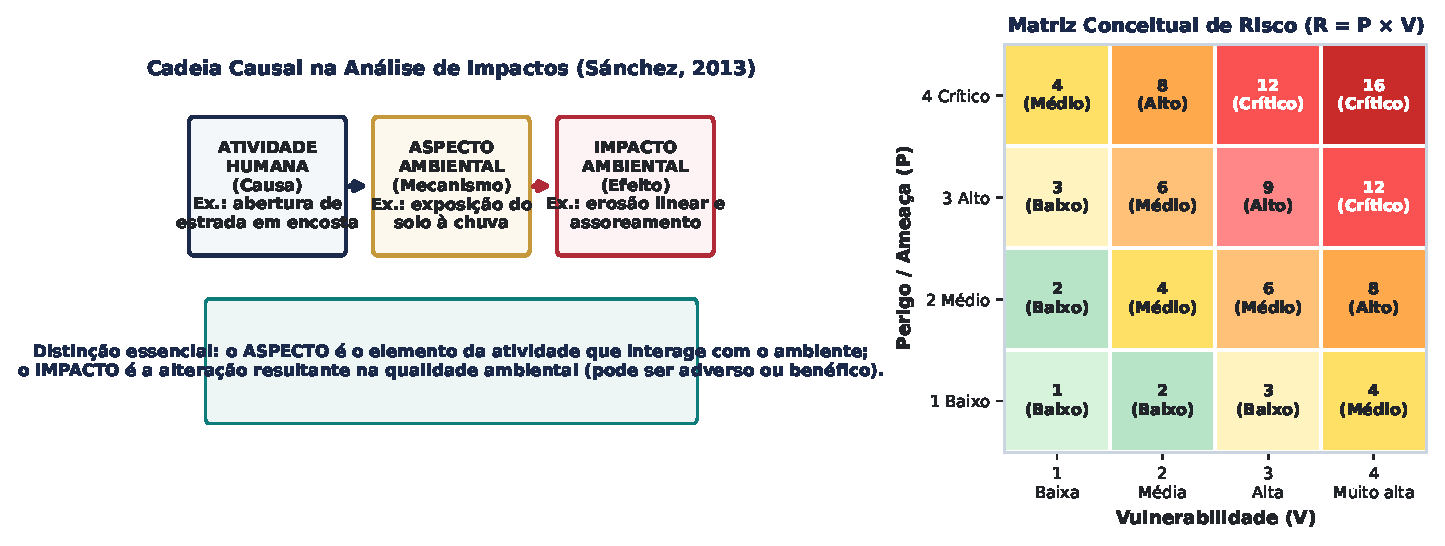
\includegraphics[width=0.95\textwidth]{figures/fig02_aspecto_impacto_risco.pdf}
  \caption{Conceitos operacionais centrais da Análise Ambiental: (a) cadeia causal Atividade Humana, Aspecto Ambiental e Impacto Ambiental segundo Sánchez (2013); (b) Matriz Conceitual de Risco Ambiental ($R = P \times V$) em escala ordinal $4 \times 4$ (Baixo, Médio, Alto e Crítico). Fonte: Elaboração didática CHF662.}
  \label{fig:aspecto-risco}
\end{figure}

Para que os impactos identificados em um diagnóstico sejam comparáveis e subsidiem medidas mitigadoras proporcionais, a Análise Ambiental classifica cada impacto segundo sete atributos operacionais (Sánchez, 2013). Quanto à \textbf{natureza (valor)}, distingue-se o impacto adverso (como erosão em sulcos após desmatamento) do benéfico (como o aumento da infiltração após bioengenharia de talude). Quanto à \textbf{ordem causal}, separa-se o impacto direto ou primário (remoção da vegetação em margem) do indireto ou secundário (assoreamento a jusante reduzindo o volume útil de um reservatório). Pelo \textbf{prazo de manifestação}, diferencia-se o efeito imediato (ruído e poeira durante uma obra) daquele de médio ou longo prazo (salinização progressiva de solo irrigado no Semiárido). Quanto à \textbf{duração}, o impacto pode ser temporário (turbidez restrita à construção de um bueiro), permanente (submersão definitiva de um vale por barragem) ou cíclico. Quanto à \textbf{reversibilidade}, distinguem-se alterações reversíveis mediante manejo (compactação superficial) daquelas irreversíveis (extinção local de espécie endêmica ou perda total de horizonte orgânico em rocha exposta). Pela \textbf{abrangência espacial}, classifica-se o efeito em local ou pontual, regional (alteração hidrológica na bacia do Rio Paraguaçu) ou estratégico. Ademais, quanto à \textbf{interação e acumulação}, o impacto \textbf{cumulativo} resulta da soma de efeitos semelhantes ao longo do tempo ou de múltiplos empreendimentos (como dezenas de pequenos barramentos reduzindo a vazão total de um rio), enquanto o impacto \textbf{sinérgico} decorre da interação entre dois ou mais impactos distintos cujo efeito combinado supera a soma isolada das partes (como supressão de mata ciliar associada ao lançamento de esgoto doméstico elevando drasticamente a eutrofização e o assoreamento). O Exemplo 4.1 aplica essa cadeia causal e sua classificação a uma obra viária urbana.

\begin{boxExemplo}{4.1 (Básico)}{Cadeia Atividade-Aspecto-Impacto e Classificação em Obra Urbana}
\passoEnunciado{A prefeitura de Feira de Santana realiza uma obra de abertura de avenida marginal com drenagem pluvial ao longo de um córrego urbano. Durante a terraplanagem em período chuvoso, máquinas retiram a vegetação de barranco sem instalar barreiras de contenção de sedimentos, gerando enxurrada barrenta que atinge o córrego e assoreia um trecho de $400\text{ m}$ a jusante. Estruture a cadeia causal e classifique o impacto de assoreamento.}
\passoDados{Obra de abertura de avenida marginal; retirada de vegetação e exposição de solo sem contenção durante chuvas; carreamento de sedimentos e assoreamento de $400\text{ m}$ do córrego a jusante.}
\passoPedido{Separar atividade, aspecto ambiental e impacto ambiental (direto e indireto), classificando o assoreamento pelos critérios de Sánchez (2013).}
\passoMetodo{Cadeia causal da Figura~\ref{fig:aspecto-risco} (Sánchez, 2013) e os sete atributos operacionais de classificação de impactos.}
\passoContas{%
\textbf{Passo 1, Cadeia causal.} A \textbf{atividade humana} é a terraplanagem para abertura da avenida marginal. O \textbf{aspecto ambiental} consiste na supressão da cobertura vegetal com exposição do solo solto à ação erosiva da chuva e carreamento de partículas para a drenagem. O \textbf{impacto ambiental direto} corresponde à erosão acelerada no talude da obra e ao aumento imediato da turbidez da água, desencadeando o \textbf{impacto ambiental indireto} de assoreamento da calha do córrego ao longo de $400\text{ m}$ a jusante, com redução da seção de escoamento e maior risco de transbordamento.\\
\textbf{Passo 2, Classificação do impacto ``assoreamento a jusante''.} O efeito apresenta natureza \textbf{adversa}, ordem causal \textbf{indireta} (decorrente da erosão no talude), prazo \textbf{imediato a médio prazo} (já nas primeiras chuvas intensas), duração \textbf{temporária a permanente} (enquanto faltarem desassoreamento e estabilização da margem), caráter \textbf{reversível} mediante manejo corretivo (contenção de taludes e remoção controlada de sedimentos), abrangência \textbf{local} ($400\text{ m}$ na microbacia urbana) e comportamento \textbf{cumulativo} ao somar-se a sedimentos de outros loteamentos na mesma bacia.}
\passoResposta{Atividade definida pela terraplanagem; Aspecto definido pela exposição de solo sem contenção; Impacto direto em erosão e turbidez; Impacto indireto em assoreamento a jusante (adverso, indireto, imediato a médio prazo, reversível mediante intervenção, local e potencialmente cumulativo).}
\passoVerificacao{A separação clara entre aspecto e impacto permite atacar a causa (instalar barreiras de contenção, biomantas e drenagem provisória sobre o solo exposto) antes que o assoreamento se consolide.}
\end{boxExemplo}

Trocar o mecanismo de interação (aspecto) pela alteração ambiental resultante (impacto) é uma das falhas mais comuns em matrizes de Avaliação de Impacto Ambiental, como aponta o Erro 1.

\begin{boxErro}[Erro 1: Confundir Aspecto Ambiental com Impacto Ambiental]
\textbf{Equívoco frequente:} listar em uma matriz de AIA o ``desmatamento'' ou o ``lançamento de esgoto'' na coluna de \textit{impactos ambientais}.

\textbf{Por que está incorreto:} desmatamento (supressão vegetal) e lançamento de esgoto são \textbf{aspectos ambientais} (mecanismos pelos quais a atividade interage com o meio). Os \textbf{impactos} são as alterações resultantes na qualidade ambiental, como perda de habitat, erosão laminar, redução do oxigênio dissolvido ou mortandade de peixes.

\textbf{Como evitar:} teste sempre a frase com o conector ``provoca'', verificando que a \textit{Atividade} gera o \textit{Aspecto}, que \textbf{provoca} o \textit{Impacto}.
\end{boxErro}

\section{Poluição versus Degradação Ambiental}

A Lei nº 6.938/1981 (Art. 3º, incisos II e III) e Sánchez (2013) estabelecem uma relação lógica precisa de gênero e espécie entre degradação ambiental e poluição. A \textbf{degradação da qualidade ambiental} corresponde ao gênero, definido como a \textit{alteração adversa} das características do meio ambiente por meio de processos físicos, químicos ou biológicos que reduzem a qualidade ecológica, a produtividade do solo, a estabilidade do relevo ou a funcionalidade dos ecossistemas. Dentro desse conjunto mais amplo situa-se a \textbf{poluição} como espécie particular, caracterizada pela degradação da qualidade ambiental resultante de atividades que prejudiquem a saúde, a segurança e o bem-estar da população, criem condições adversas às atividades sociais e econômicas, afetem desfavoravelmente a biota ou as condições estéticas e sanitárias do meio ambiente, ou \textit{lancem matérias ou energia em desacordo com os padrões ambientais estabelecidos}.

Na prática pericial, \textbf{toda poluição causa degradação ambiental, enquanto a degradação ambiental também ocorre sem lançamento de poluentes}. Assim, o desmatamento ilegal de uma encosta de Caatinga seguido de sobrepastejo provoca compactação do solo, perda de biodiversidade e erosão em ravinas, configurando severa \textbf{degradação ambiental} mesmo na ausência de substâncias tóxicas ou poluentes químicos. Já o despejo de efluente industrial com metais pesados em um córrego acima dos padrões do CONAMA caracteriza simultaneamente \textbf{poluição} e \textbf{degradação ambiental}. O Exemplo 4.2 aplica essa distinção a duas propriedades rurais vizinhas.

\begin{boxExemplo}{4.2 (Básico)}{Poluição vs. Degradação Ambiental em Duas Propriedades no Semiárido}
\passoEnunciado{Durante fiscalização técnica em uma sub-bacia do Semiárido baiano, um analista avalia duas propriedades rurais vizinhas. Na Propriedade Alfa, o superpastejo contínuo removeu o estrato herbáceo, compactou o solo e desencadeou sulcos e ravinas profundas em encosta. Na Propriedade Beta, um pequeno laticínio lança soro de leite e água de lavagem sem tratamento diretamente em um riacho intermitente, elevando a Demanda Bioquímica de Oxigênio (DBO) muito acima dos limites do CONAMA e provocando mortandade de peixes nas poças remanescentes. Classifique cada situação quanto a degradação ambiental e poluição.}
\passoDados{Propriedade Alfa com superpastejo, solo compactado e erosão em ravinas sem lançamento de substâncias químicas ou efluentes. Propriedade Beta com lançamento de efluente orgânico fora dos padrões legais, elevação de DBO e mortandade de peixes.}
\passoPedido{Determinar, com base na Lei nº 6.938/1981 e em Sánchez (2013), se cada caso caracteriza degradação ambiental, poluição ou ambos.}
\passoMetodo{Aplicação dos incisos II e III do Art. 3º da PNMA (gênero dado pela degradação e espécie dada pela poluição).}
\passoContas{%
\textbf{Passo 1, Análise da Propriedade Alfa.} Ocorre alteração adversa severa das propriedades físicas e ecológicas do solo (compactação, perda de cobertura e erosão em ravinas), sem lançamento de substância poluente em desacordo com padrões de emissão. Caracteriza-se, portanto, \textbf{degradação ambiental} sem poluição em sentido estrito.\\
\textbf{Passo 2, Análise da Propriedade Beta.} Ocorre lançamento de matéria orgânica em desacordo com os padrões ambientais vigentes, afetando desfavoravelmente a biota (mortandade de peixes) e as condições sanitárias da água. Como toda poluição constitui uma forma específica de degradação, o caso reúne simultaneamente \textbf{poluição hídrica} e \textbf{degradação ambiental}.}
\passoResposta{Propriedade Alfa apresenta degradação ambiental sem poluição. Propriedade Beta apresenta poluição hídrica e, consequentemente, degradação ambiental.}
\passoVerificacao{O enquadramento jurídico e técnico está consistente com a relação de inclusão da PNMA ($\text{poluição} \subset \text{degradação}$), orientando respostas distintas, como manejo conservacionista do solo e pastagem em Alfa e estação de tratamento de efluentes com autuação por poluição em Beta.}
\end{boxExemplo}

Igualar poluição e degradação ou negar a existência de impactos positivos gera enquadramentos jurídicos equivocados, como detalhado no Erro 2.

\begin{boxErro}[Erro 2: Tratar Todo Impacto como Negativo e Igualar Poluição a Degradação]
\textbf{Equívoco frequente:} afirmar que ``não há impacto ambiental em projetos de recuperação'' ou dizer que ``a erosão do solo por pastoreio é um caso de poluição''.

\textbf{Por que está incorreto:} projetos de recuperação geram \textbf{impactos ambientais benéficos} (positivos); além disso, erosão sem lançamento de substâncias em desacordo com padrões legais constitui \textbf{degradação ambiental}, distinguindo-se de poluição.

\textbf{Como evitar:} qualifique sempre o impacto (adverso ou benéfico) e verifique se houve lançamento de matéria ou energia ou alteração sanitária prevista no Art. 3º, III da PNMA antes de usar o termo poluição.
\end{boxErro}

\section{Perigo, Vulnerabilidade, Fragilidade Ambiental e Risco Ambiental}

Quatro conceitos frequentemente confundidos em relatórios técnicos precisam ser rigorosamente separados para fundamentar mapas de risco, defesa civil e ordenamento territorial, cuja lógica matricial foi introduzida na Subfigura (b) da Figura~\ref{fig:aspecto-risco}. O \textbf{perigo ou ameaça ($P$)} designa o evento ou fenômeno físico, biológico ou tecnológico com potencial intrínseco de causar dano a pessoas, bens ou ecossistemas (como chuva extrema concentrada, escorregamento translacional em encosta, inundação brusca ou rompimento de barragem), referindo-se à \textit{probabilidade e intensidade do evento potencialmente danoso}.

Diante dessa ameaça, a \textbf{vulnerabilidade ($V$)} mede o grau de exposição, suscetibilidade e incapacidade de proteção, resposta ou recuperação de uma população, edificação, infraestrutura ou atividade econômica. Trata-se de um atributo com forte componente socioespacial, pois famílias com moradias precárias em fundos de vale sem drenagem nem alerta precoce apresentam vulnerabilidade muito superior à de edificações estruturadas fora da cota de inundação diante da mesma chuva. Já a \textbf{fragilidade ambiental} expressa uma propriedade física e ecológica intrínseca de um ambiente ou unidade de paisagem de sofrer desestabilização frente a processos morfodinâmicos e intervenções humanas, em função da interação entre declividade, solo, litologia, clima e cobertura vegetal (conceito formalizado no Cap.~9 com a metodologia de Ross, 1994), subsistindo mesmo quando falta ocupação humana.

Dessa articulação emerge o \textbf{risco ambiental ($R$)}, entendido como a expectativa de perdas ou danos resultante da interseção entre um \textbf{perigo ($P$)} e um sistema \textbf{vulnerável ($V$)}. A distinção entre fragilidade física e risco socioambiental evidencia-se quando comparamos duas encostas com idêntica declividade de $38\%$ e solo raso (Figura~\ref{fig:risco_vs_fragilidade}). Enquanto a Vertente~1 permanece conservada e sem população exposta ($V = 0 \Rightarrow R = 0$), na Vertente~2 o desmatamento e a ocupação irregular na base elevam o perigo e a vulnerabilidade até o risco crítico ($R = 16$).

\begin{figure}[H]
  \centering
  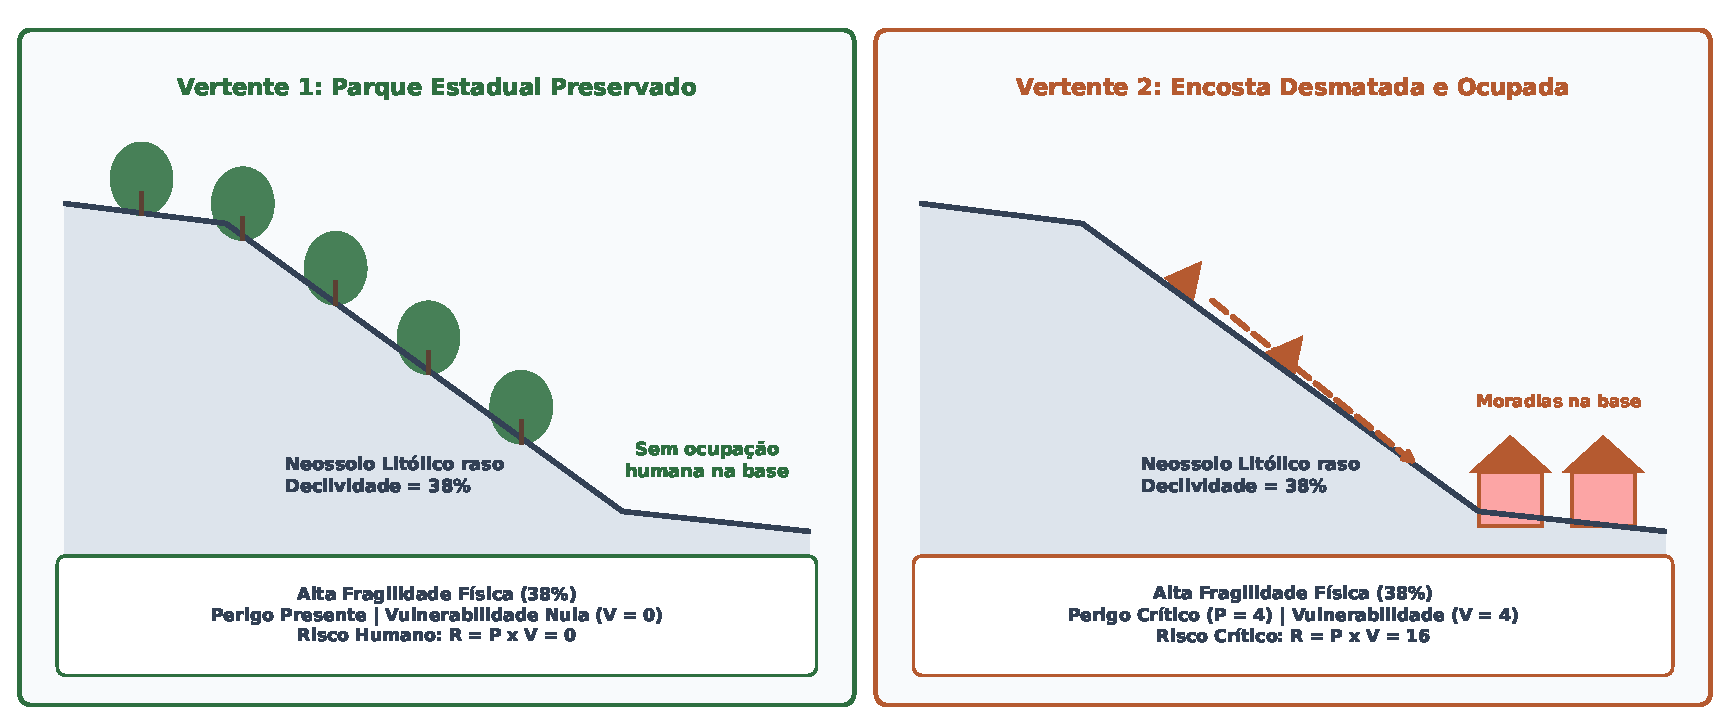
\includegraphics[width=0.95\textwidth]{figures/fig_cap04_risco_vs_fragilidade.pdf}
  \caption{Distinção operacional entre fragilidade física, perigo, vulnerabilidade e risco ($R = P \times V$) em duas encostas com mesma declividade de 38\% e solo raso, contrastando risco humano nulo na Vertente 1 ($V = 0$) e risco crítico na Vertente 2 ($R = 16$). Fonte: Elaboração didática CHF662.}
  \label{fig:risco_vs_fragilidade}
\end{figure}

Na análise semiquantitativa de riscos socioambientais alinhada à matriz $4 \times 4$ da Subfigura (b) da Figura~\ref{fig:aspecto-risco}, o índice de risco ambiental $R$ resulta do produto entre o nível de perigo ($P$) e o nível de vulnerabilidade ($V$), servindo a redução relativa $\Delta R\%$ para medir o efeito de intervenções preventivas ou mitigadoras. Quando as variáveis são ordinais, o produto $R$ opera como convenção de priorização de gestão, orientando decisões conforme as faixas de risco sem representar probabilidade numérica direta de ocorrência.

\begin{boxFormula}[Equação e Variação Percentual do Risco Ambiental ($R = P \times V$)]
\begin{align}
  R &= P \times V \\
  \Delta R\% &= \frac{R_{\text{final}} - R_{\text{inicial}}}{R_{\text{inicial}}} \times 100\%
\end{align}
Nestas expressões, $P \in \{1, 2, 3, 4\}$ representa o nível de Perigo ($1 = \text{Baixo}$, $2 = \text{Médio}$, $3 = \text{Alto}$, $4 = \text{Crítico}$) e $V \in \{0, 1, 2, 3, 4\}$ indica a Vulnerabilidade ($0 = \text{Nula}$ por ausência de exposição, $1 = \text{Baixa}$, $2 = \text{Média}$, $3 = \text{Alta}$, $4 = \text{Muito alta}$). Os valores de $R$ ($0$ a $16$) agrupam-se nas classes \textbf{Baixo} ($1 \le R \le 3$), \textbf{Médio} ($4 \le R \le 6$), \textbf{Alto} ($8 \le R \le 9$) e \textbf{Crítico} ($R \ge 12$).
\end{boxFormula}

O Exemplo 4.3 demonstra o cálculo matricial do risco em três setores de encosta e quantifica a redução percentual alcançada após obras de drenagem, bioengenharia e realocação.

\begin{boxExemplo}{4.3 (Intermediário)}{Cálculo Matricial e Redução Percentual de Risco Ambiental ($R = P \times V$)}
\passoEnunciado{A Defesa Civil de um município do Recôncavo Baiano mapeou três setores de uma vertente sujeita a escorregamentos (Setores A, B e C) utilizando a matriz $4 \times 4$ da Figura~\ref{fig:aspecto-risco}. Posteriormente, no setor mais grave, a prefeitura executou obras de drenagem superficial, estabilização de talude com bioengenharia e realocação das casas mais precárias. Avalie o risco inicial de cada setor e quantifique o efeito percentual da intervenção.}
\passoDados{Cenário inicial com Setor A ($P = 4$, $V = 4$), Setor B ($P = 3$, $V = 3$) e Setor C ($P = 4$, $V = 1$). Cenário pós-intervenção no Setor A com perigo reduzido de $4$ para $3$ (drenagem e estabilização) e vulnerabilidade reduzida de $4$ para $2$ (realocação e reforço estrutural).}
\passoPedido{Calcular $R = P \times V$ e classificar os setores A, B e C antes da obra, determinando também o novo risco de A e a variação percentual $\Delta R\%$.}
\passoMetodo{Aplicação da equação $R = P \times V$, das faixas da Figura~\ref{fig:aspecto-risco} (1--3 Baixo; 4--6 Médio; 8--9 Alto; 12--16 Crítico) e de $\Delta R\% = \frac{R_1 - R_0}{R_0}\times 100\%$.}
\passoContas{%
\textbf{Passo 1, Cálculo inicial dos três setores.} No Setor A, $R_A = 4 \times 4 = 16$ (\textbf{Risco Crítico}); no Setor B, $R_B = 3 \times 3 = 9$ (\textbf{Risco Alto}); no Setor C, $R_C = 4 \times 1 = 4$ (\textbf{Risco Médio}).\\
\textbf{Passo 2, Comparação crítica entre B e C.} Embora o Setor C possua perigo maior ($P = 4$) do que o Setor B ($P = 3$), seu risco ($R_C = 4$) corresponde a menos da metade do risco de B ($R_B = 9$) porque a vulnerabilidade em C é baixa ($V = 1$).\\
\textbf{Passo 3, Cenário pós-intervenção no Setor A ($P_1 = 3$, $V_1 = 2$).}
\[
R_{A,\text{final}} = 3 \times 2 = 6 \quad (\textbf{Risco Médio}).
\]
\textbf{Passo 4, Variação percentual do risco no Setor A.}
\[
\Delta R\% = \frac{6 - 16}{16} \times 100\% = \frac{-10}{16} \times 100\% = -0{,}625 \times 100\% = -62{,}50\%.
\]}
\passoResposta{Inicialmente, Setor A = $16$ (Crítico), Setor B = $9$ (Alto) e Setor C = $4$ (Médio). Após intervenção no Setor A, $R = 6$ (Médio), representando redução de $62{,}50\%$ no índice de risco.}
\passoVerificacao{O resultado faz pleno sentido matemático ($6/16 = 37{,}5\%$ do risco original, logo queda de $62{,}5\%$) e operacional, demonstrando que atuar simultaneamente sobre o perigo (engenharia e bioengenharia) e sobre a vulnerabilidade (ordenamento e habitação) produz queda acentuada de risco.}
\end{boxExemplo}

Rotular mapas puramente físicos de declividade ou erodibilidade como mapas de risco ignora a dimensão de exposição humana, equívoco alertado a seguir.

\begin{boxErro}[Erro 3: Confundir Fragilidade Ambiental ou Perigo com Risco]
\textbf{Equívoco frequente:} chamar um mapa de declividade ou de erodibilidade de ``mapa de risco ambiental'' sem considerar a presença e a vulnerabilidade da população ou da infraestrutura.

\textbf{Por que está incorreto:} declividade e erodibilidade expressam \textbf{fragilidade} ou \textbf{perigo físico ($P$)}. Sem vulnerabilidade ($V > 0$), falta exposição capaz de gerar risco socioambiental ($R = P \times V$).

\textbf{Como evitar:} verifique se os dois fatores ($P$ e $V$) estão explicitamente presentes no diagnóstico antes de empregar a palavra risco.
\end{boxErro}

O Exemplo 4.4 consolida a separação entre fragilidade potencial, perigo, vulnerabilidade e risco em duas vertentes idênticas da Caatinga sob usos distintos do solo.

\begin{boxExemplo}{4.4 (Intermediário)}{Fragilidade Ambiental vs. Perigo vs. Risco em Vertentes da Caatinga}
\passoEnunciado{Considere duas vertentes geomorfologicamente idênticas no Semiárido baiano, ambas com $38\%$ de declividade, Neossolo Litólico raso e chuvas concentradas de alta erosividade. A Vertente 1 localiza-se no interior de um Parque Estadual preservado, sem estradas nem moradores. A Vertente 2 teve sua vegetação suprimida e recebeu um loteamento residencial irregular na base da encosta. Compare fragilidade ambiental, perigo, vulnerabilidade e risco nas duas vertentes.}
\passoDados{Vertente 1 com declividade $38\%$, solo raso, vegetação de Caatinga preservada e ausência de população ou bens expostos. Vertente 2 com mesma declividade e solo, vegetação suprimida e loteamento irregular na base.}
\passoPedido{Diferenciar conceitualmente a condição de cada vertente quanto a fragilidade potencial, perigo, vulnerabilidade e risco socioambiental.}
\passoMetodo{Distinção rigorosa entre fragilidade intrínseca do meio físico, ameaça física, exposição humana e risco conforme a Seção 4.4.}
\passoContas{%
\textbf{Passo 1, Fragilidade potencial (meio físico).} Ambas as vertentes apresentam \textbf{alta fragilidade natural potencial}, pois compartilham declividade elevada ($38\%$), solo raso e chuvas erosivas. Na Vertente 1, a cobertura vegetal conservada protege o solo (menor fragilidade emergente); na Vertente 2, a supressão vegetal eleva a instabilidade.\\
\textbf{Passo 2, Perigo ou Ameaça ($P$).} Em ambas existe potencial físico de escoamento rápido e queda de material, acentuado na Vertente 2 pela retirada da vegetação e pelos cortes de talude do loteamento.\\
\textbf{Passo 3, Vulnerabilidade ($V$).} Na Vertente 1, faltam pessoas, habitações ou infraestruturas expostas ($V = 0$ do ponto de vista socioambiental humano). Na Vertente 2, há moradias precárias diretamente na zona de impacto ($V$ alta ou muito alta).\\
\textbf{Passo 4, Risco Socioambiental ($R$).} Na Vertente 1, apesar da alta fragilidade física, o risco de desastre humano é \textbf{nulo} ($R = P \times 0 = 0$). Na Vertente 2, a convergência entre alto perigo e alta vulnerabilidade gera \textbf{risco alto ou crítico}.}
\passoResposta{Ambas possuem alta fragilidade física potencial, porém apenas a Vertente 2 apresenta risco socioambiental humano elevado, em virtude da exposição de moradores vulneráveis e da desestabilização antrópica da cobertura vegetal.}
\passoVerificacao{Esse contraste comprova por que mapas de fragilidade física exigem o cruzamento com dados de exposição e vulnerabilidade social antes de receberem o rótulo de ``mapas de risco''.}
\end{boxExemplo}

\section{Resiliência, Recuperação, Restauração, Reabilitação e Sustentabilidade}

Quando um ambiente já sofreu degradação, o analista ambiental precisa avaliar sua capacidade de resposta espontânea e definir o objetivo técnico viável de intervenção, articulando os limiares de tolerância da matriz de risco às trajetórias de resiliência do sistema (Figura~\ref{fig:matriz_risco_tolerancia}). Enquanto níveis baixos de risco ($R \le 3$) demandam monitoramento e níveis médios ($4 \le R \le 6$) requerem controle preventivo, situações de risco alto ($8$ a $9$) exigem mitigação prioritária e riscos críticos ($\ge 12$) impõem intervenção imediata, pois o sistema aproxima-se do limiar de ruptura estrutural.

O ponto de partida dessa avaliação é a \textbf{resiliência}, entendida como a capacidade de um ecossistema ou sistema socioambiental absorver perturbações dentro da faixa de resistência elástica, reorganizar-se e retornar ao estado funcional quando cessa a pressão. Quando a perda de horizontes férteis A e B, a compactação severa ou a incisão em ravinas ultrapassam o \textbf{limiar crítico de ruptura} (ponto de não retorno), o sistema ingressa em um novo estado degradado marcado por \textbf{histerese} (Figura~\ref{fig:matriz_risco_tolerancia}), no qual a mera retirada do fator de pressão falha em recompor o ambiente espontaneamente, exigindo PRAD e bioengenharia.

\begin{figure}[H]
  \centering
  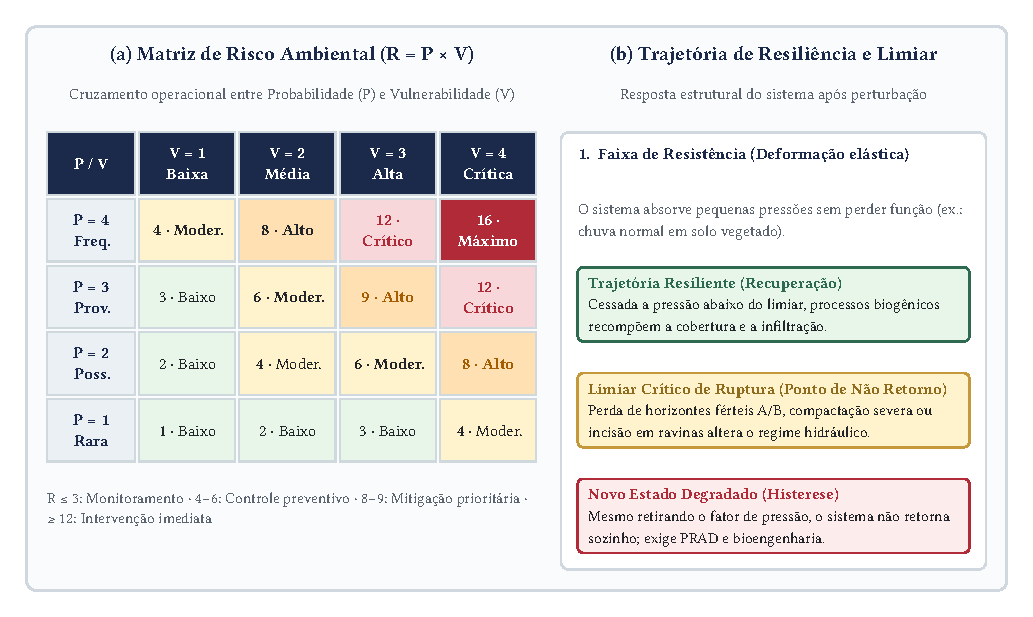
\includegraphics[width=0.95\textwidth]{figures/fig_cap04_matriz_risco_tolerancia.pdf}
  \caption{Articulação entre classes de tolerância e ação na Matriz de Risco Ambiental ($R = P \times V$, Painel (a)) e trajetória de resiliência, limiar crítico de ruptura e histerese após degradação severa (Painel (b)). Fonte: Elaboração didática CHF662.}
  \label{fig:matriz_risco_tolerancia}
\end{figure}

Quando a intervenção humana se torna necessária, Sánchez (2013) e a Lei do SNUC (Lei nº 9.985/2000, Art. 2º, incisos XIII e XIV) diferenciam estratégias com metas técnicas precisas. A \textbf{recuperação ambiental} opera como conceito guarda-chuva técnico e legal adotado em PRAD e licenciamento, designando a restituição de um ecossistema degradado a uma \textit{condição não degradada} que pode igualar-se ou diferir da condição original. Dentro desse espectro, a \textbf{restauração ecológica} representa o objetivo mais exigente, buscando restituir a estrutura, a composição de espécies nativas e as funções ecológicas o mais próximo possível da \textit{condição original pré-distúrbio}, meta indicada para APPs, nascentes e Unidades de Conservação onde a resiliência e os remanescentes permitem recomposição nativa. Já a \textbf{reabilitação ambiental} conduz a área degradada a um estado estável, seguro e funcional voltado a um \textit{novo uso predefinido} (produtivo, urbano, paisagístico ou de lazer) em locais muito alterados, como cavas urbanas ou antigas pedreiras em que o retorno ao estado original é inviável física ou economicamente. Em situações com passivos químicos por hidrocarbonetos, chorume, metais pesados ou agrotóxicos persistentes, aplica-se a \textbf{remediação} (Sánchez, 2013), voltada a remover, conter ou neutralizar contaminantes no solo e na água subterrânea.

Articulando essas escalas no longo prazo, a \textbf{sustentabilidade} atua como princípio orientador que mantém o uso dos recursos naturais dentro da capacidade de suporte e regeneração dos ecossistemas, integrando integridade ecológica, viabilidade econômica, justiça socioespacial e equidade intergeracional. Na literatura ambiental, distingue-se a \textit{sustentabilidade fraca}, que admite substituir capital natural por capital financeiro ou tecnológico, da \textit{sustentabilidade forte}, que reconhece funções ecológicas críticas insubstituíveis, como água doce, solos férteis e biodiversidade.

% ============================================================================
% ETAPA 4 - SÍNTESE AVANÇADA E ESTUDO DE CASO INTEGRADOR
% ============================================================================
\etapa{4}{Síntese Avançada: Resiliência, Sinergia e Escolha de Estratégia em PRAD}

Passivos ambientais severos frequentemente combinam baixa resiliência física, ruptura topográfica irreversível e pressões difusas provenientes do entorno urbano ou agrícola. O Exemplo 4.5 integra os conceitos de resiliência, impacto sinérgico e escolha técnica entre restauração e reabilitação para fundamentar um Plano de Recuperação de Áreas Degradadas.

\begin{boxExemplo}{4.5 (Avançado)}{Escolha entre Restauração e Reabilitação em Passivo Minerário}
\passoEnunciado{Na planície fluvial do Rio Jacuípe (BA), uma área de $8\text{ ha}$ usada por 15 anos para extração irregular de areia deixou cavas com $4\text{ m}$ de profundidade que atingiram o lençol freático, margens instáveis em desmoronamento e perda completa do horizonte A do solo. A área está hoje cercada por expansão urbana e por pequenas lavouras que aplicam fertilizantes solúveis. O Ministério Público exigiu um PRAD. Discuta a resiliência local, o potencial impacto cumulativo e sinérgico com as lavouras vizinhas e justifique tecnicamente a escolha entre restauração ecológica integral e reabilitação ambiental.}
\passoDados{Passivo de $8\text{ ha}$ com cavas de $4\text{ m}$ atingindo o lençol freático, margens instáveis, ausência de solo superficial, entorno urbano e agrícola com fertilizantes e exigência legal de PRAD.}
\passoPedido{Avaliar a resiliência do sistema, a possibilidade de impacto sinérgico com o entorno e a estratégia mais adequada entre restauração e reabilitação.}
\passoMetodo{Critérios de resiliência, impactos cumulativos e sinérgicos e distinção entre recuperação, restauração e reabilitação segundo Sánchez (2013) e Lei do SNUC.}
\passoContas{%
\textbf{Passo 1, Avaliação da resiliência.} A resiliência natural está severamente comprometida (\textbf{muito baixa}). A remoção de $4\text{ m}$ de sedimento eliminou o horizonte superficial, a matéria orgânica e o banco de sementes, alterando irreversivelmente a topografia e expondo a água subterrânea em condição de histerese na qual a regeneração espontânea falha em restituir a floresta ciliar original.\\
\textbf{Passo 2, Impacto sinérgico com as lavouras.} O escoamento superficial carregando nutrientes das lavouras vizinhas (aspecto agrícola) encontra o lençol freático exposto nas cavas estagnadas (aspecto minerário). A combinação desses dois processos distintos gera eutrofização acelerada e risco de contaminação do aquífero, efeito mais intenso do que cada atividade isolada (\textbf{impacto sinérgico}).\\
\textbf{Passo 3, Escolha entre restauração e reabilitação.} A \textbf{restauração ecológica integral} (retorno exato à planície original pré-mineração) exigiria milhões de metros cúbicos de material de aterro externo, criando novas áreas degradadas de empréstimo e tornando-se ambiental e economicamente inviável. A estratégia tecnicamente recomendada é a \textbf{reabilitação ambiental} (inserida no guarda-chuva legal da recuperação), promovendo retaludamento e estabilização das margens das cavas com bioengenharia, implantação de faixa tampão de vegetação nativa ciliar para filtrar nutrientes das lavouras e conversão das lagoas estabilizadas em parque ecológico e área segura de amortecimento hídrico.}
\passoResposta{Resiliência muito baixa; risco de impacto sinérgico (eutrofização e contaminação do aquífero pela interação entre cava aberta e fertilizantes); a estratégia indicada é a \textbf{reabilitação ambiental} associada à faixa tampão vegetada nativa nas bordas, descartando a restauração topográfica integral por inviabilidade física e ecológica.}
\passoVerificacao{A decisão respeita a legislação (o PRAD exige recuperação, que admite reabilitação quando o retorno ao estado original é impraticável) e neutraliza tanto a instabilidade geotécnica das margens quanto a vulnerabilidade do lençol freático.}
\end{boxExemplo}

% ============================================================================
% ETAPA 5 - ARMADILHA CONCEITUAL E MATERIAIS AUDIOVISUAIS DE APOIO
% ============================================================================
\etapa{5}{Armadilha Conceitual e Materiais Audiovisuais de Apoio}

Ao redigir planos de recuperação ou condicionar licenciamentos, um equívoco recorrente consiste em prometer metas tecnicamente inviáveis por confundir o significado jurídico de recuperação, restauração e reabilitação.

\begin{boxErro}[Erro 4: Prometer ``Restauração Integral'' Onde Apenas a Reabilitação é Viável]
\textbf{Equívoco frequente:} redigir em um PRAD que uma cava profunda de mineração ou uma área urbana aterrada será ``integralmente restaurada à sua condição original''.

\textbf{Por que está incorreto:} a restauração exige aproximação máxima da estrutura, composição e funções originais pré-distúrbio, o que frequentemente se torna impossível após alterações geomorfológicas irreversíveis. Promessas inexequíveis levam à rejeição do PRAD ou ao descumprimento de condicionantes.

\textbf{Como evitar:} avalie a resiliência e o grau de alteração do relevo e do solo; adote a \textbf{restauração} apenas quando o retorno ao ecossistema de referência for factível, e a \textbf{reabilitação} quando o objetivo for um novo uso estável e seguro.
\end{boxErro}

Para aprofundar a compreensão integrada dos conceitos de degradação, vulnerabilidade, fragilidade e resiliência ambiental aplicados a estudos técnicos, assista à videoaula recomendada na página da disciplina, intitulada \textit{Degradação Ambiental} (\url{https://www.youtube.com/watch?v=5EFxN7jGob8}), que revisa esses conceitos operacionais e suas implicações para o planejamento e a recuperação de áreas degradadas.

% ============================================================================
% ETAPA 6 - EXERCÍCIOS DE FIXAÇÃO (15 EXERCÍCIOS EM 3 NÍVEIS)
% ============================================================================
\etapa{6}{Exercícios de Fixação}

\subsection*{Nível Básico (Exercícios 1 a 5)}

\begin{enumerate}[leftmargin=1.8em, itemsep=4pt]
  \item Apresente a definição legal de \textbf{meio ambiente} segundo a Lei nº 6.938/1981 (PNMA) e explique por que Sánchez (2013) recomenda incluir explicitamente o meio construído e as relações socioeconômicas na Análise Ambiental.
  \espacoResolucao[2.0cm]

  \item Para a atividade humana ``operação de uma indústria cerâmica de pequeno porte'', cite um exemplo de \textbf{aspecto ambiental} e um exemplo do correspondente \textbf{impacto ambiental}.
  \espacoResolucao[2.0cm]

  \item Explique a diferença entre \textbf{impacto cumulativo} e \textbf{impacto sinérgico}, apresentando um exemplo prático para cada um em uma bacia hidrográfica.
  \espacoResolucao[2.0cm]

  \item Justifique a afirmação segundo a qual toda poluição provoca degradação ambiental, embora a degradação ambiental também ocorra sem poluição.
  \espacoResolucao[2.0cm]

  \item Defina \textbf{resiliência ambiental} e explique por que um solo decapado até a rocha apresenta resiliência muito menor do que uma pastagem abandonada cercada por fragmentos de mata nativa.
  \espacoResolucao[2.0cm]
\end{enumerate}

\subsection*{Nível Intermediário (Exercícios 6 a 10)}

\begin{enumerate}[leftmargin=1.8em, itemsep=4pt, resume]
  \item Uma encosta ocupada (Encosta X) foi avaliada inicialmente com Perigo Alto ($P_0 = 3$) e Vulnerabilidade Muito Alta ($V_0 = 4$). Após obras de retaludamento, drenagem pluvial e melhoria estrutural das moradias, os indicadores caíram para Perigo Médio ($P_1 = 2$) e Vulnerabilidade Média ($V_1 = 2$). Calcule passo a passo o risco inicial $R_0$ e sua classe, o risco final $R_1$ e sua classe, e a variação percentual $\Delta R\%$.
  \espacoResolucao[2.8cm]

  \item Compare duas margens de rio urbano usando a matriz $4 \times 4$ da Figura~\ref{fig:aspecto-risco}, considerando que a \textbf{Margem Y} tem $P = 4$ e $V = 3$, enquanto a \textbf{Margem Z} tem $P = 3$ e $V = 2$. Determine o índice e a classe de risco de cada margem e indique qual delas deve receber prioridade emergencial de intervenção, justificando.
  \espacoResolucao[2.3cm]

  \item A implantação de uma Estação de Tratamento de Esgoto (ETE) municipal gera ruído temporário durante os 8 meses de obras, mas, após entrar em operação, reduz em $85\%$ a carga orgânica lançada no rio local durante décadas. Classifique esses dois impactos segundo os critérios de \textbf{natureza}, \textbf{duração} e \textbf{reversibilidade}.
  \espacoResolucao[2.3cm]

  \item Diferencie \textbf{fragilidade ambiental}, \textbf{perigo} e \textbf{risco} no contexto de um paredão rochoso instável localizado em área desabitada de parque estadual e, em comparação, imediatamente acima de uma rodovia federal movimentada.
  \espacoResolucao[2.3cm]

  \item Uma pedreira de granito desativada na periferia de uma cidade média do Nordeste possui paredões verticais de $18\text{ m}$ e piso totalmente rochoso. Entre \textbf{restauração ecológica} e \textbf{reabilitação ambiental}, qual alternativa é tecnicamente mais adequada? Justifique sua escolha.
  \espacoResolucao[2.3cm]
\end{enumerate}

\subsection*{Nível Aplicado: Questões Objetivas (Exercícios 11 a 15)}

\begin{enumerate}[leftmargin=1.8em, itemsep=5pt, resume]
  \item Na cadeia causal apresentada por Sánchez (2013) e na Figura~\ref{fig:aspecto-risco}, ao analisar a atividade ``aplicação de fertilizantes em área agrícola declivosa'', constitui um \textbf{aspecto ambiental} e o seu respectivo \textbf{impacto ambiental}, nessa ordem:
  \begin{alternativas}
    \item Eutrofização do açude; carreamento de nitrogênio e fósforo pela enxurrada.
    \item Carreamento de nutrientes pela enxurrada para o corpo d'água; eutrofização do açude e proliferação de algas.
    \item Aplicação de fertilizantes; compra de insumos agrícolas.
    \item Proliferação de algas; abertura de estrada rural.
    \item Redução do oxigênio dissolvido; emissão de licença ambiental.
  \end{alternativas}
  \espacoResolucao[1.2cm]

  \item Em uma bacia hidrográfica do Semiárido, cinco pequenas indústrias lançam efluentes tratados dentro do padrão individual, mas a soma das cargas ao longo do rio reduz gradualmente a qualidade da água na foz. Esse fenômeno caracteriza um impacto tipicamente:
  \begin{alternativas}
    \item Benéfico e pontual.
    \item Irreversível e imediato apenas na fonte.
    \item Cumulativo.
    \item Natural e sem origem antrópica.
    \item Estético sem alteração físico-química.
  \end{alternativas}
  \espacoResolucao[1.2cm]

  \item Segundo a Matriz Conceitual de Risco ($R = P \times V$, escala $1$ a $4$ da Figura~\ref{fig:aspecto-risco}), uma área classificada com Perigo Crítico ($P = 4$) e Vulnerabilidade Baixa ($V = 1$) apresenta:
  \begin{alternativas}
    \item $R = 16$ (Risco Crítico).
    \item $R = 12$ (Risco Crítico).
    \item $R = 8$ (Risco Alto).
    \item $R = 4$ (Risco Médio).
    \item $R = 2$ (Risco Baixo).
  \end{alternativas}
  \espacoResolucao[1.2cm]

  \item De acordo com a Lei do SNUC (Lei nº 9.985/2000) e com Sánchez (2013), a restituição de um ecossistema degradado a uma condição \textbf{o mais próximo possível da sua condição original} denomina-se:
  \begin{alternativas}
    \item Remediação.
    \item Reabilitação.
    \item Restauração.
    \item Compensação financeira.
    \item Mitigação preventiva.
  \end{alternativas}
  \espacoResolucao[1.2cm]

  \item Sobre o conceito de \textbf{sustentabilidade forte}, em contraste com a sustentabilidade fraca, é correto afirmar que:
  \begin{alternativas}
    \item Admite substituir integralmente ecossistemas críticos por capital financeiro ou infraestrutura artificial.
    \item Reconhece que determinadas funções ecológicas e estoques naturais críticos (como água doce, solos férteis e biodiversidade) são insubstituíveis e impõem limites biofísicos ao crescimento econômico.
    \item Aplica-se exclusivamente a unidades de conservação sem presença humana no entorno.
    \item Desconsidera a justiça social e a dimensão intergeracional na gestão ambiental.
    \item Equivale à compensação pecuniária automática de qualquer dano irreversível.
  \end{alternativas}
  \espacoResolucao[1.2cm]
\end{enumerate}

% ============================================================================
% ETAPA 7 - QUESTÕES ESTILO ENADE E CONCURSOS AMBIENTAIS
% ============================================================================
\etapa{7}{Questões no Estilo ENADE e Concursos Ambientais}

\begin{boxDica}[Estratégia para o Estudo Orientado 3 (EO3) e para a Avaliação Teórica]
No \textbf{EO3} (Semana 4, baseado em Sánchez, 2013, cap. 1, e Tauk-Tornisielo, 1996) e em concursos para Analista Ambiental (IBAMA, ICMBio e INEMA), há três pegadinhas recorrentes que você agora sabe desarmar:
\begin{enumerate}[leftmargin=1.5em, itemsep=1.5pt]
  \item \textbf{Aspecto $\neq$ Impacto,} identificando sempre se o enunciado descreve o mecanismo de interação (aspecto) ou a mudança no estado do meio (impacto).
  \item \textbf{Degradação $\supset$ Poluição,} verificando se houve lançamento de poluente ou alteração sanitária prevista em lei ou apenas degradação física e ecológica (como erosão e desmatamento).
  \item \textbf{Restauração $\neq$ Reabilitação $\neq$ Recuperação,} lembrando que \textit{recuperação} é o termo geral (condição não degradada, igual ou diferente da original), enquanto \textit{restauração} busca o estado original e \textit{reabilitação} destina a área a um novo uso funcional estável.
\end{enumerate}
\end{boxDica}

\begin{enumerate}[leftmargin=1.8em, itemsep=5pt, start=16]
  \item \textbf{(Questão autoral, estilo Concurso Analista Ambiental / IBAMA)} Com base na Política Nacional do Meio Ambiente (Lei nº 6.938/1981), na Resolução CONAMA nº 01/1986 e na obra de Sánchez (2013), julgue as proposições abaixo:
  \begin{enumerate}[label=\Roman*., leftmargin=2.0em, itemsep=2pt]
    \item Um impacto ambiental é necessariamente negativo, razão pela qual programas de recuperação florestal deixam de produzir impactos ambientais.
    \item A remoção da vegetação ciliar com consequente assoreamento de curso d'água constitui degradação ambiental mesmo na ausência de lançamento de efluentes químicos tóxicos.
    \item A interação entre dois impactos distintos cujo efeito conjunto supera a soma de seus efeitos isolados define o caráter sinérgico do impacto.
    \item A exposição do solo decorrente da abertura de uma estrada é o aspecto ambiental, enquanto a perda de solo por erosão laminar e o aumento da turbidez no córrego são os impactos ambientais.
  \end{enumerate}
  Estão corretas apenas as proposições:
  \begin{alternativas}
    \item I e II.
    \item I e III.
    \item II e IV.
    \item II, III e IV.
    \item I, II, III e IV.
  \end{alternativas}
  \espacoResolucao[1.3cm]

  \item \textbf{(Questão autoral, estilo ENADE / Geografia)} Duas comunidades localizam-se na mesma bacia hidrográfica semiárida, submetidas a eventos de enxurrada súbita de igual intensidade (mesmo perigo físico $P = 3$). A Comunidade 1 possui sistema de drenagem pluvial, construções em alvenaria fora da cota máxima de cheia e plano de alerta comunitário ($V = 1$). A Comunidade 2 ocupa precariamente a planície de inundação, sem drenagem nem alerta ($V = 4$). À luz dos conceitos operacionais de perigo, vulnerabilidade e risco ($R = P \times V$), assinale a alternativa correta:
  \begin{alternativas}
    \item Ambas as comunidades possuem o mesmo risco ambiental, pois estão expostas à mesma intensidade pluviométrica ($P = 3$).
    \item A Comunidade 1 apresenta risco baixo ($R = 3$) e a Comunidade 2 apresenta risco crítico ($R = 12$), demonstrando o peso determinante da vulnerabilidade socioespacial na produção de desastres.
    \item A Comunidade 2 apresenta risco médio ($R = 7$), resultado da soma entre perigo ($3$) e vulnerabilidade ($4$).
    \item A vulnerabilidade é uma propriedade estritamente geológica do terreno, independente da renda, da infraestrutura e da localização das moradias.
    \item Para reduzir o risco da Comunidade 2, a única medida tecnicamente possível consiste em modificar o regime climático regional para eliminar a chuva intensa.
  \end{alternativas}
  \espacoResolucao[1.3cm]

  \item \textbf{(Questão autoral, estilo Concurso Perito Ambiental / INEMA)} Um empreendimento de extração de argila abandonou, há dez anos, uma área de $12\text{ ha}$ sem solo superficial, com cavas alagadas e taludes instáveis em periferia urbana. O laudo pericial constatou resiliência natural muito baixa e propôs estabilizar os taludes, revegetar as margens com espécies nativas e integrar o espelho d'água a um parque urbano de retenção de cheias, deixando claro que a reconstituição do relevo e da floresta originais mostra-se inviável. Conceitualmente, a intervenção proposta corresponde à:
  \begin{alternativas}
    \item Restauração ecológica integral, pois utiliza espécies nativas nas margens.
    \item Remediação química, visto que a área estava abandonada há dez anos.
    \item Reabilitação ambiental, modalidade de recuperação que destina a área degradada a um novo uso estável e funcional distinto da condição original.
    \item Degradação controlada, uma vez que preserva a modificação topográfica prévia.
    \item Sustentabilidade fraca ilegal, pois o SNUC proíbe qualquer intervenção que deixe de reconstituir integralmente o estado original.
  \end{alternativas}
  \espacoResolucao[1.3cm]
\end{enumerate}

% ============================================================================
% ETAPA 8 - GABARITO INTEGRALMENTE COMENTADO (EM PÁGINA SEPARADA)
% ============================================================================
\clearpage
\etapa{8}{Gabarito Integralmente Comentado (Exercícios 1 a 18)}

\begin{boxGabarito}[Resolução: Nível Básico (Exercícios 1 a 5)]
\begin{enumerate}[leftmargin=1.8em, itemsep=4pt]
  \item \textbf{Meio ambiente (PNMA e Sánchez, 2013).} Pela Lei nº 6.938/1981 (Art. 3º, I), meio ambiente é o conjunto de condições, leis, influências e interações de ordem física, química e biológica que permite, abriga e rege a vida em todas as suas formas. Sánchez (2013) destaca a inclusão do meio construído e das relações socioeconômicas porque as atividades humanas transformam continuamente os sistemas naturais e os impactos ambientais atingem diretamente a saúde, a economia, o patrimônio e o bem-estar social (como reconhece a Resolução CONAMA nº 01/1986).
  \item \textbf{Indústria cerâmica (aspecto e impacto).} Um exemplo de \textit{aspecto ambiental} é a emissão de fumaça e material particulado pela queima de lenha nos fornos (ou extração de argila em várzea), provocando o \textit{impacto ambiental} de degradação da qualidade do ar e agravo a doenças respiratórias no entorno (ou desestabilização de margens e perda de vegetação ciliar).
  \item \textbf{Cumulativo e Sinérgico.} O impacto \textit{cumulativo} resulta da soma de impactos semelhantes ao longo do tempo ou de diversas fontes (como múltiplos barramentos rurais em uma bacia reduzindo progressivamente a vazão no exutório). O impacto \textit{sinérgico} resulta da interação entre dois ou mais impactos distintos cujo efeito combinado supera a soma isolada das partes (como remoção de mata ciliar somada ao lançamento de esgoto doméstico, acelerando conjuntamente o assoreamento e a eutrofização severa do rio).
  \item \textbf{Poluição $\subset$ Degradação.} Pela PNMA (Art. 3º, II e III), degradação é o gênero (qualquer alteração adversa do meio), enquanto poluição é uma espécie específica de degradação (ligada a prejuízos à saúde, biota ou bem-estar ou lançamento de matéria e energia fora dos padrões). Logo, toda poluição degrada o ambiente, ao passo que processos como desmatamento, compactação e erosão degradam o ambiente sem envolver poluição química.
  \item \textbf{Resiliência.} Capacidade do sistema absorver perturbações e recuperar estrutura e funções essenciais. O solo decapado até a rocha perdeu horizonte orgânico, estrutura porosa, retenção hídrica e banco de sementes (resiliência muito baixa, próxima ao quadro de histerese); já a pastagem cercada por fragmentos nativos preserva solo e fonte próxima de propágulos (sementes e dispersores), conferindo resiliência muito mais alta.
\end{enumerate}
\end{boxGabarito}

\begin{boxGabarito}[Resolução: Nível Intermediário (Exercícios 6 a 10)]
\begin{enumerate}[leftmargin=1.8em, itemsep=4pt, start=6]
  \item \textbf{Cálculo passo a passo do risco na Encosta X.}
  O risco inicial é $R_0 = P_0 \times V_0 = 3 \times 4 = \mathbf{12}$ (\textbf{Risco Crítico}, pois $R \ge 12$). O risco final reduz-se a $R_1 = P_1 \times V_1 = 2 \times 2 = \mathbf{4}$ (\textbf{Risco Médio}, faixa $4 \le R \le 6$). A variação percentual resulta em
  \[
  \Delta R\% = \frac{R_1 - R_0}{R_0} \times 100\% = \frac{4 - 12}{12} \times 100\% = \frac{-8}{12} \times 100\% = -\frac{2}{3} \times 100\% \approx \mathbf{-66{,}67\%}.
  \]
  A intervenção reduziu o índice de risco em $66{,}67\%$, deslocando a encosta da classe Crítica para a classe Média.
  \item \textbf{Comparação Margem Y e Margem Z.}
  A Margem Y alcança $R_Y = 4 \times 3 = \mathbf{12}$ (\textbf{Risco Crítico}), enquanto a Margem Z registra $R_Z = 3 \times 2 = \mathbf{6}$ (\textbf{Risco Médio}). A \textbf{Margem Y} deve receber intervenção emergencial prioritária, pois possui o dobro do índice de risco de Z e encontra-se na faixa crítica ($R = 12$).
  \item \textbf{Classificação dos impactos da ETE.}
  O ruído durante 8 meses de obras apresenta natureza \textbf{adversa}, duração \textbf{temporária} e caráter \textbf{reversível} (cessando ao término da obra). A redução de $85\%$ da carga orgânica no rio apresenta natureza \textbf{benéfica}, duração \textbf{permanente} (enquanto a ETE operar adequadamente) e caráter \textbf{reversível} caso a estação deixe de receber manutenção.
  \item \textbf{Paredão rochoso instável.}
  No parque desabitado, há alta \textbf{fragilidade} física e existência de \textbf{perigo} de queda de blocos ($P > 0$), porém faltam elementos humanos expostos ($V = 0$), resultando em \textbf{risco humano nulo}. Acima da rodovia movimentada, mantêm-se a mesma fragilidade e perigo físico, agora combinados com alta exposição de veículos e passageiros ($V > 0$), configurando \textbf{risco socioambiental elevado} que exige obras de contenção e monitoramento.
  \item \textbf{Pedreira de granito desativada.} A estratégia tecnicamente adequada é a \textbf{reabilitação ambiental}. A remoção de $18\text{ m}$ de maciço rochoso alterou irreversivelmente a topografia e eliminou o solo original, tornando inviável a restauração ecológica à condição pré-mineração. A reabilitação permite estabilizar os paredões, drenar a cava e criar um uso seguro (como parque geológico, anfiteatro ou área de lazer com vegetação rupestre adaptada).
\end{enumerate}
\end{boxGabarito}

\begin{boxGabarito}[Resolução: Nível Aplicado e Estilo ENADE/Concursos (Exercícios 11 a 18)]
\begin{enumerate}[leftmargin=1.8em, itemsep=3.5pt, start=11]
  \item \textbf{Gabarito: (B).} O carreamento de nutrientes pela enxurrada é o mecanismo de interação com o meio (\textit{aspecto}), enquanto a eutrofização e a proliferação de algas representam a alteração na qualidade da água (\textit{impacto}). A alternativa (A) inverte causa e efeito.
  \item \textbf{Gabarito: (C).} A soma de múltiplas contribuições semelhantes ao longo do rio que deteriora gradualmente a qualidade hídrica na foz define o \textbf{impacto cumulativo}.
  \item \textbf{Gabarito: (D).} Pela fórmula $R = P \times V$, temos $R = 4 \times 1 = 4$. Na matriz $4 \times 4$ da Figura~\ref{fig:aspecto-risco}, valores entre $4$ e $6$ correspondem à classe \textbf{Risco Médio}.
  \item \textbf{Gabarito: (C).} A Lei do SNUC (Art. 2º, XIV) define \textbf{restauração} exatamente como a restituição de um ecossistema ou população silvestre degradada o mais próximo possível de sua condição original.
  \item \textbf{Gabarito: (B).} A \textbf{sustentabilidade forte} recusa a substituibilidade plena entre capital natural e capital financeiro, afirmando que funções ecológicas críticas (água, solo e biodiversidade) impõem limites biofísicos reais.
  \item \textbf{Gabarito: (D).} A proposição I é falsa porque impactos ambientais podem ser benéficos (como em programas de recuperação florestal). As proposições II (degradação sem poluente químico), III (definição exata de sinergia) e IV (distinção correta entre aspecto e impacto) estão integralmente corretas.
  \item \textbf{Gabarito: (B).} Comunidade 1 obtém $R_1 = 3 \times 1 = 3$ (Risco Baixo), e Comunidade 2 atinge $R_2 = 3 \times 4 = 12$ (Risco Crítico). Mesmo sob igual perigo ($P = 3$), a vulnerabilidade socioespacial quadruplicou o índice de risco. As demais alternativas usam soma como operação matricial, reduzem vulnerabilidade à geologia ou ignoram medidas de proteção social.
  \item \textbf{Gabarito: (C).} Como a área será estabilizada e destinada a um novo uso funcional (parque de retenção de cheias) sem reconstituição da condição original, trata-se de \textbf{reabilitação ambiental}, uma modalidade legítima de recuperação prevista no escopo de um PRAD.
\end{enumerate}
\end{boxGabarito}

% ============================================================================
% ETAPA 9 - RESUMO DO CAPÍTULO
% ============================================================================
\begin{boxResumo}
\begin{itemize}[leftmargin=1.5em, itemsep=2.2pt]
  \item \textbf{Ambiente,} sistema de interações físico-químicas, bióticas e socioeconômicas (Lei nº 6.938/1981; CONAMA nº 01/1986; Sánchez, 2013).
  \item \textbf{Cadeia Causal,} a Atividade Humana (causa) gera o Aspecto Ambiental (mecanismo), que provoca o Impacto Ambiental (efeito adverso ou benéfico).
  \item \textbf{Atributos dos Impactos,} natureza (adverso ou benéfico), ordem (direto ou indireto), prazo (imediato, médio ou longo), duração (temporário ou permanente), reversibilidade, abrangência espacial, cumulatividade e sinergia.
  \item \textbf{Poluição e Degradação,} degradação é o gênero (toda alteração adversa); poluição é espécie (degradação associada a danos sanitários ou bióticos ou lançamento de matéria e energia fora dos padrões).
  \item \textbf{Fragilidade, Perigo, Vulnerabilidade e Risco,} fragilidade é intrínseca ao sistema biofísico; risco exige interseção entre perigo ($P$) e vulnerabilidade ($V$), calculado na matriz $4 \times 4$ por $R = P \times V$ ($1$--$3$ Baixo; $4$--$6$ Médio; $8$--$9$ Alto; $12$--$16$ Crítico).
  \item \textbf{Resiliência e Intervenção,} \textit{recuperação} (condição não degradada, termo geral) engloba \textit{restauração} (próximo ao original) e \textit{reabilitação} (novo uso funcional estável); \textit{remediação} trata contaminantes químicos; \textit{sustentabilidade forte} respeita limites ecológicos insubstituíveis e evita cruzar o limiar de histerese.
\end{itemize}
\end{boxResumo}

% ============================================================================
% ETAPA 10 - TESTE DE APRENDIZAGEM (CHECKPOINT)
% ============================================================================
\begin{boxTeste}
Responda sem consultar o texto e verifique o gabarito logo abaixo.
\begin{enumerate}[leftmargin=1.6em, itemsep=3pt]
  \item (\textbf{V ou F}) Na Resolução CONAMA nº 01/1986 e em Sánchez (2013), o conceito de impacto ambiental aplica-se exclusivamente a alterações negativas provocadas por atividades industriais.
  \item (\textbf{V ou F}) A compactação do solo e a erosão em sulcos causadas por manejo inadequado de pastagem constituem degradação ambiental, mesmo na ausência de lançamento de poluentes químicos.
  \item \textbf{Cálculo rápido,} na matriz $R = P \times V$ ($1$ a $4$), uma área com $P = 3$ e $V = 3$ recebe qual valor e qual classe de risco? Se a vulnerabilidade for reduzida para $V = 2$ (mantendo $P = 3$), qual será o novo risco e sua classe?
  \item \textbf{Enquadramento técnico,} qual é a diferença central de objetivo entre \textbf{restauração} e \textbf{reabilitação} ambiental?
\end{enumerate}
\vspace{3pt}
\hrule
\vspace{4pt}
{\footnotesize\textbf{Gabarito do Checkpoint:}
\textbf{1.} \F\ (impacto pode ser adverso ou benéfico e resultar de qualquer atividade humana, abrangendo também obras e serviços). \quad
\textbf{2.} \V\ (degradação é o gênero amplo; poluição é espécie particular). \quad
\textbf{3.} Inicial $R = 3 \times 3 = \mathbf{9}$ (\textbf{Risco Alto}); final $R = 3 \times 2 = \mathbf{6}$ (\textbf{Risco Médio}). \quad
\textbf{4.} A \textbf{restauração} busca restituir o ecossistema o mais próximo possível de sua condição original pré-distúrbio; a \textbf{reabilitação} destina a área degradada a um novo uso estável e funcional diferente do original.}
\end{boxTeste}

% ============================================================================
% SIMULADO E REVISÃO INTEGRADA DO MÓDULO 1 (CAPÍTULOS 1 A 4)
% Componente: CHF662 — Análise Ambiental (DCHF/UEFS)
% Vínculo no Plano CHF662: Revisão EO1–EO3 e Preparação para Prova Teórica
% ============================================================================

\clearpage
\phantomsection
\addcontentsline{toc}{chapter}{Simulado e Revisão Integrada: Módulo 1}
\chapter*{Simulado e Revisão Integrada: Módulo 1}
\markboth{SIMULADO DO MÓDULO 1}{SIMULADO DO MÓDULO 1}

\noindent\tagEmenta\ \tagEO{1}\ \tagEO{2}\ \tagEO{3}

\vspace{6pt}

\begin{boxConceito}[Instruções de Aplicação e Alinhamento Avaliativo]
Este simulado integra os conteúdos dos \textbf{Capítulos 1 a 4} (Semanas 1 a 4 do Plano CHF662), preparando diretamente para a consolidação dos \textbf{Estudos Orientados (EO1, EO2 e EO3)} e para a \textbf{Avaliação Teórica Individual} (Semana 10).
\begin{itemize}[leftmargin=1.5em, itemsep=2pt]
  \item \textbf{Tempo sugerido:} 90 minutos (50 minutos para as 8 questões objetivas + 40 minutos para as 2 questões dissertativas).
  \item \textbf{Modo de estudo:} resolva todas as questões sem consulta. Ao concluir, utilize o \textbf{Gabarito Integralmente Comentado}, o \textbf{Espelho Dissertativo} e a \textbf{Tabela de Diagnóstico de Revisão} na página seguinte para identificar exatamente quais capítulos revisar.
  \item \textbf{Pontuação simulada (escala $0$ a $10,0$):} Questões 1 a 8 valem $0,75$ ponto cada ($6,0$ pontos); Questões 9 e 10 valem $2,0$ pontos cada ($4,0$ pontos).
\end{itemize}
\end{boxConceito}

% ============================================================================
% PARTE I — QUESTÕES OBJETIVAS CONTEXTUALIZADAS (1 A 8)
% ============================================================================
\section*{Parte I: Questões Objetivas (Estilo ENADE e Concursos Ambientais)}

\begin{enumerate}[leftmargin=1.8em, itemsep=6pt]

  \item \textbf{(Cap. 1, Questão autoral, estilo ENADE / Geografia)} Ao discutir a crise ambiental contemporânea, Enrique Leff (2001) sustenta que a degradação generalizada dos solos, a escassez hídrica e a perda de biodiversidade não podem ser solucionadas apenas por ajustes tecnológicos pontuais. De acordo com essa perspectiva epistemológica, a crise ambiental contemporânea caracteriza-se fundamentalmente como:
  \begin{alternativas}
    \item Um ciclo climático puramente geológico, independente das formas de organização econômica e técnica da humanidade.
    \item Uma crise civilizatória e de racionalidade científica e econômica, produzida por um modelo que fragmentou o saber e tratou a natureza como recurso ilimitado.
    \item Um desequilíbrio restrito a países de clima semiárido, solucionável apenas pela importação de tecnologia de irrigação intensiva.
    \item Uma consequência inevitável do crescimento demográfico absoluto, desvinculada dos padrões de consumo e da desigualdade territorial.
    \item Um problema estritamente jurídico, cuja resolução depende apenas da ampliação do valor das multas administrativas sem mudança produtiva.
  \end{alternativas}
  \espacoResolucao[1.2cm]

  \item \textbf{(Caps. 1 e 2, Questão autoral, estilo ENADE / Geografia)} Carlos Walter Porto-Gonçalves (2006) analisa como o pensamento moderno consolidou a ideia de ``natureza'' como algo externo à humanidade, passível de domínio técnico irrestrito. Sobre as consequências dessa concepção moderna na relação sociedade--natureza, assinale a alternativa correta:
  \begin{alternativas}
    \item A modernidade integrou plenamente os saberes tradicionais e os ciclos ecológicos locais ao ritmo de acumulação industrial.
    \item A noção de natureza é universal e imutável em todas as culturas, não sofrendo influência histórica, política ou simbólica.
    \item A separação sujeito--objeto legitimou a apropriação mercantil dos recursos naturais e invisibilizou modos de vida de populações que se concebem como parte dos ecossistemas.
    \item A Geografia moderna surgiu para rejeitar completamente o estudo da materialidade natural em favor da filosofia abstrata.
    \item A concepção moderna eliminou os conflitos socioambientais ao garantir distribuição homogênea de água e terra no espaço rural brasileiro.
  \end{alternativas}
  \espacoResolucao[1.2cm]

  \item \textbf{(Cap. 2, Questão autoral, estilo Concurso Analista Ambiental / INEMA)} Em uma região do Semiárido baiano, a instalação de um empreendimento minerário de grande porte alterou o acesso de comunidades tradicionais de fundo de pasto a aguadas comunitárias e áreas de uso coletivo da Caatinga. A empresa classificou a reação comunitária como ``entrave cultural ao progresso''. À luz do debate sobre conflitos socioambientais (Porto-Gonçalves, 2006; Mendonça, 2001), esse episódio expressa:
  \begin{alternativas}
    \item Um conflito socioambiental territorial, no qual distintos grupos sociais disputam a apropriação material, simbólica e decisória da base ecológica local.
    \item Uma divergência puramente técnica que deve ser resolvida sem participação social, bastando apresentar mapas geológicos do minério.
    \item Um problema restrito à Geografia Física, pois envolve apenas a recarga hídrica subterrânea das aguadas.
    \item Uma comprovação do determinismo ambiental, visto que o clima semiárido impede qualquer convivência produtiva sustentável.
    \item Um impacto exclusivamente natural, sem relação com modelos de desenvolvimento ou desigualdade de poder.
  \end{alternativas}
  \espacoResolucao[1.2cm]

  \item \textbf{(Cap. 3, Questão autoral, estilo ENADE / Geografia)} Sobre a proposta da \textbf{Geografia Socioambiental} formulada por Francisco Mendonça (2001) e sua posição frente à história do pensamento geográfico moderno, avalie as afirmações a seguir:
  \begin{enumerate}[label=\Roman*., leftmargin=2.0em, itemsep=2pt]
    \item A proposta surge como resposta crítica à dicotomia entre uma Geografia Física excessivamente naturalista e uma Geografia Humana que secundarizou a materialidade ecológica.
    \item O prefixo ``socio'' indica que os problemas ambientais resultam da interação indissociável entre processos biofísicos e organização social, política e econômica.
    \item A abordagem socioambiental recomenda que o relatório de diagnóstico seja dividido em anexos isolados de meio físico e meio humano sem cruzamento causal, para preservar a neutralidade de cada ramo.
  \end{enumerate}
  É correto o que se afirma apenas em:
  \begin{alternativas}
    \item I.
    \item II.
    \item I e II.
    \item II e III.
    \item I, II e III.
  \end{alternativas}
  \espacoResolucao[1.2cm]

  \item \textbf{(Cap. 3, Questão autoral, estilo Concurso Geógrafo / Planejamento Ambiental)} No diagnóstico integrado de uma microbacia urbana com lagoas assoreadas em Feira de Santana (BA), uma equipe aplicou o \textbf{Sistema Tripolar GTP} de Georges Bertrand (2004). Assinale a alternativa que associa corretamente um procedimento de campo ao respectivo polo do sistema:
  \begin{alternativas}
    \item Levantamento de escrituras, legislação de APP e disputas imobiliárias $\rightarrow$ Polo Geossistema (G).
    \item Medição da taxa de infiltração do solo, balanço hídrico e transporte de sedimentos sob influência da impermeabilização urbana $\rightarrow$ Polo Geossistema (G).
    \item Entrevistas sobre memória afetiva das lagoas e valorização simbólica do espelho d'água pelos moradores antigos $\rightarrow$ Polo Território (T).
    \item Mapeamento de declividade e granulometria dos sedimentos depositados no fundo da lagoa $\rightarrow$ Polo Paisagem (P), por tratar-se de dinâmica estritamente cultural.
    \item Fiscalização de loteamentos irregulares pela secretaria municipal de meio ambiente $\rightarrow$ Polo Paisagem (P), por envolver a estética dos muros urbanos.
  \end{alternativas}
  \espacoResolucao[1.2cm]

  \item \textbf{(Cap. 4, Questão autoral, estilo Concurso Analista Ambiental / IBAMA)} Durante a implantação de uma linha de transmissão elétrica atravessando vertentes íngremes e cursos d'água, a supressão da mata ciliar somou-se à compactação do solo por maquinário pesado. Essa combinação intensificou o escoamento concentrado e provocou ravinas muito mais profundas do que ocorreria se apenas um dos dois processos atuasse isoladamente. Conforme Sánchez (2013) e a Resolução CONAMA nº 01/1986, é correto afirmar que:
  \begin{alternativas}
    \item A formação de ravinas é o aspecto ambiental, enquanto a supressão da mata ciliar e a compactação são os impactos ambientais.
    \item O agravamento desproporcional resultante da interação entre dois processos distintos exemplifica o caráter \textbf{sinérgico} do impacto ambiental.
    \item Por não envolver lançamento de produto químico tóxico, a erosão em ravinas não constitui degradação ambiental nem impacto ambiental.
    \item A obra produz apenas impactos permanentes e irreversíveis, não sendo possível adotar medidas mitigadoras ou de recuperação.
    \item O impacto descrito classifica-se como benéfico e indireto, por ampliar a visibilidade dos afloramentos rochosos na bacia.
  \end{alternativas}
  \espacoResolucao[1.2cm]

  \item \textbf{(Cap. 4, Questão autoral, estilo Concurso Defesa Civil / Gestão de Riscos)} Um município baiano aplicou a matriz conceitual de risco ambiental $R = P \times V$ (escala ordinal de $1$ a $4$, com classes: $1$--$3$ Baixo; $4$--$6$ Médio; $8$--$9$ Alto; $12$--$16$ Crítico) a quatro setores de encosta e fundo de vale, obtendo os seguintes dados:
  \begin{center}
  \renewcommand{\arraystretch}{1.15}
  \small
  \begin{tabular}{@{}lcc@{}}
    \toprule
    \rowcolor{uefsNavy}
    \textcolor{white}{\bfseries Setor Avaliado} & \textcolor{white}{\bfseries Perigo ($P$)} & \textcolor{white}{\bfseries Vulnerabilidade ($V$)} \\
    \midrule
    Setor I (encosta íngreme ocupada sem drenagem) & $4$ & $4$ \\
    \rowcolor{bgGray}
    Setor II (margem de córrego com ocupação consolidada precária) & $3$ & $3$ \\
    Setor III (encosta muito íngreme com vegetação preservada e acesso restrito) & $4$ & $1$ \\
    \rowcolor{bgGray}
    Setor IV (área de baixa declividade com moradias de vulnerabilidade alta) & $2$ & $3$ \\
    \bottomrule
  \end{tabular}
  \end{center}
  Com base no cálculo exato de $R = P \times V$, assinale a alternativa correta:
  \begin{alternativas}
    \item Os Setores I e III pertencem ambos à classe Crítica, pois compartilham $P = 4$.
    \item O Setor II ($R = 9$, Alto) apresenta risco inferior ao do Setor IV ($R = 6$, Médio).
    \item O Setor I apresenta risco Crítico ($R = 16$), o Setor II apresenta risco Alto ($R = 9$), e os Setores III ($R = 4$) e IV ($R = 6$) enquadram-se na classe de risco Médio.
    \item A ordem decrescente de prioridade técnica de intervenção é: Setor I $>$ Setor III $>$ Setor II $>$ Setor IV.
    \item O Setor III deve ser classificado como Risco Baixo ($R = 4$) porque sua vulnerabilidade é igual a $1$.
  \end{alternativas}
  \espacoResolucao[1.5cm]

  \item \textbf{(Cap. 4, Questão autoral, estilo Concurso Perito Ambiental / IBAMA--INEMA)} Uma antiga área de mineração de cascalho em encosta do Semiárido sofreu decapagem completa do solo e rebaixamento topográfico de $6\text{ m}$, apresentando resiliência natural muito baixa. O órgão ambiental exige um PRAD que elimine a erosão ativa, estabilize os taludes e permita o aproveitamento seguro do terreno como viveiro comunitário de mudas nativas e área de captação de água pluvial, reconhecendo a impossibilidade física de reconstituir o relevo e a vegetação originais. O conceito operacional que define corretamente essa estratégia é:
  \begin{alternativas}
    \item Restauração ecológica integral.
    \item Poluição controlada.
    \item Reabilitação ambiental (enquadrada no conceito amplo de recuperação).
    \item Fragilidade potencial nula.
    \item Remediação química de metais pesados.
  \end{alternativas}
  \espacoResolucao[1.2cm]

\end{enumerate}

% ============================================================================
% PARTE II — QUESTÕES DISSERTATIVAS PREPARATÓRIAS (9 E 10)
% ============================================================================
\section*{Parte II: Questões Dissertativas (Preparação para EO1--EO3 e Prova Teórica)}

\begin{enumerate}[leftmargin=1.8em, itemsep=6pt, start=9]

  \item \textbf{(Integração Caps. 1, 2 e 3, Preparatória para EO1, EO2 e Prova Teórica)} Em uma microbacia do Semiárido baiano, a expansão de atividades intensivas sem planejamento desencadeou conflitos pelo uso da água, desmatamento de cabeceiras e perda de referência cultural dos moradores com o riacho local. Redija um texto técnico articulado (15 a 22 linhas) explicando:
  \begin{enumerate}[label=(\alph*), leftmargin=1.8em, itemsep=1.5pt]
    \item Como a crise ambiental nesse caso reflete a ruptura moderna entre sociedade e natureza (Leff, 2001; Porto-Gonçalves, 2006);
    \item Por que a Geografia Socioambiental (Mendonça, 2001) supera os limites das análises puramente naturalistas ou exclusivamente sociais;
    \item Como o \textbf{Sistema Tripolar GTP} de Georges Bertrand (2004) organizaria o diagnóstico integrado dessa microbacia nos polos Geossistema (G), Território (T) e Paisagem (P).
  \end{enumerate}
  \espacoResolucao[4.4cm]

  \item \textbf{(Integração Caps. 3 e 4, Preparatória para EO3 e Prova Teórica)} Durante a abertura de uma estrada de acesso em vertente declivosa da Caatinga sem sistema de drenagem, o solo exposto sofreu ravinamento severo e sedimentos foram carreados para um açude comunitário situado na base da encosta, onde vivem famílias dependentes da água armazenada. Com base em Sánchez (2013) e Tauk-Tornisielo (1996):
  \begin{enumerate}[label=(\alph*), leftmargin=1.8em, itemsep=1.5pt]
    \item Decomponha a cadeia causal identificando \textbf{atividade}, \textbf{aspecto ambiental}, \textbf{impacto direto} e \textbf{impacto indireto};
    \item Esclareça se o assoreamento do açude por sedimentos erodidos configura degradação ambiental, poluição ou ambos, justificando com base na PNMA;
    \item Considere que, no Cenário 1 (sem drenagem nem contenção), a área de jusante apresenta Perigo Crítico ($P_1 = 4$) e Vulnerabilidade Alta ($V_1 = 3$). No Cenário 2 (após implantação de drenagem, paliçadas retentoras de sedimentos e proteção das margens do açude), o perigo cai para Médio ($P_2 = 2$) e a vulnerabilidade para Média ($V_2 = 2$). Calcule $R_1$, $R_2$, suas respectivas classes na matriz $4 \times 4$ e a variação percentual $\Delta R\%$;
    \item Indique se a recomposição das margens do açude (APP) deve priorizar \textbf{restauração} ou \textbf{reabilitação}, justificando sua resposta.
  \end{enumerate}
  \espacoResolucao[4.4cm]

\end{enumerate}

% ============================================================================
% GABARITO INTEGRALMENTE COMENTADO, ESPELHO E TABELA DE DIAGNÓSTICO
% ============================================================================
\clearpage
\section*{Parte III: Gabarito Integralmente Comentado (Questões 1 a 8)}

\begin{boxGabarito}[Análise Comentada das Questões Objetivas]
\begin{enumerate}[leftmargin=1.8em, itemsep=4pt]
  \item \textbf{Gabarito: (B).} Para Enrique Leff (2001), a crise ambiental é uma crise civilizatória e de racionalidade (epistemológica e econômica) derivada da fragmentação do conhecimento e da lógica de acumulação que ignora limites ecológicos. \textit{Distratores:} (A) naturaliza a crise; (C) reduz a questão ao clima semiárido; (D) reproduz neomalthusianismo simplista; (E) reduz o problema a multas administrativas.
  \item \textbf{Gabarito: (C).} Porto-Gonçalves (2006) demonstra que a separação moderna sujeito--objeto transformou a natureza em objeto externo e mercadoria, deslegitimando saberes e territorialidades de povos integrados aos ecossistemas. \textit{Distratores:} (A) e (E) invertem o processo histórico; (B) naturaliza uma categoria histórica; (D) distorce a história da Geografia.
  \item \textbf{Gabarito: (A).} A disputa por aguadas e terras de uso coletivo envolvendo empresas e comunidades tradicionais caracteriza um conflito socioambiental territorial (apropriação material, simbólica e poder decisório). \textit{Distratores:} (B), (C) e (E) despolitizam e fragmentam o fenômeno; (D) ressuscita o determinismo ambiental.
  \item \textbf{Gabarito: (C).} As afirmações I e II reproduzem fielmente os fundamentos da Geografia Socioambiental em Mendonça (2001). A afirmação III é falsa porque anexos isolados sem cruzamento causal caracterizam a multidisciplinaridade justaposta que a Geografia Socioambiental busca superar.
  \item \textbf{Gabarito: (B).} Taxa de infiltração, balanço hídrico e transporte de sedimentos (incluindo o efeito físico da impermeabilização urbana) pertencem ao polo \textbf{Geossistema (G)}. \textit{Distratores:} (A) descreve Território, não G; (C) descreve Paisagem, não T; (D) descreve Geossistema, não P; (E) descreve Território, não P.
  \item \textbf{Gabarito: (B).} Quando dois processos distintos (supressão de mata ciliar + compactação por máquinas) interagem gerando efeito maior do que a soma isolada das partes, o impacto é \textbf{sinérgico}. \textit{Distratores:} (A) inverte aspecto e impacto; (C) confunde degradação com poluição química; (D) ignora a mitigação/recuperação; (E) classifica erroneamente como benéfico.
  \item \textbf{Gabarito: (C).} Cálculos passo a passo na matriz $R = P \times V$:
  \begin{itemize}[leftmargin=1.4em, itemsep=1pt]
    \item Setor I: $R_{\text{I}} = 4 \times 4 = 16$ (\textbf{Crítico});
    \item Setor II: $R_{\text{II}} = 3 \times 3 = 9$ (\textbf{Alto});
    \item Setor III: $R_{\text{III}} = 4 \times 1 = 4$ (\textbf{Médio});
    \item Setor IV: $R_{\text{IV}} = 2 \times 3 = 6$ (\textbf{Médio}).
  \end{itemize}
  Ordem decrescente real: $\text{I} (16) > \text{II} (9) > \text{IV} (6) > \text{III} (4)$. \textit{Distratores:} (A) ignora $V=1$ no Setor III; (B) inverte $9$ e $6$; (D) erra a ordem entre II, III e IV; (E) classifica $R = 4$ como Baixo (a faixa Baixo vai de $1$ a $3$).
  \item \textbf{Gabarito: (C).} Como a área possui resiliência muito baixa e alteração topográfica irreversível, sendo destinada a um novo uso produtivo e seguro (viveiro e captação pluvial), aplica-se a \textbf{reabilitação ambiental} (modalidade de recuperação). \textit{Distratores:} (A) restauração exigiria aproximação da condição original; (B) não se trata de poluição; (D) e (E) são conceitos incompatíveis com o caso.
\end{enumerate}
\end{boxGabarito}

\section*{Parte IV: Espelho Dissertativo e Rubrica de Correção (Questões 9 e 10)}

\begin{boxGabarito}[Espelho Dissertativo: Questão 9 (Valor: 2,0 pontos)]
\textbf{Eixos obrigatórios e pontuação:}
\begin{itemize}[leftmargin=1.5em, itemsep=2pt]
  \item \textbf{Item (a), Ruptura sociedade--natureza (0,6 pt):} explicitar que a crise local não é mera falha técnica ou destino climático, mas reflexo da racionalidade econômica e científica moderna que separou sociedade e natureza (Leff, 2001; Porto-Gonçalves, 2006), tratando água e vegetação como insumos apropriáveis de forma desigual.
  \item \textbf{Item (b), Geografia Socioambiental (0,6 pt):} demonstrar que a análise puramente naturalista oculta os conflitos pelo uso da água e as decisões econômicas, enquanto a análise exclusivamente social omite o funcionamento hidrológico e a degradação das cabeceiras; a Geografia Socioambiental (Mendonça, 2001) integra ambas as dimensões como unidade inseparável.
  \item \textbf{Item (c), Aplicação do Sistema GTP (0,8 pt):} organizar claramente os três polos de Bertrand (2004) e suas interações: \textbf{G (Geossistema)}, balanço hídrico, infiltração, desmatamento de cabeceiras e erosão; \textbf{T (Território)}, outorga/disputa pelo uso da água, estrutura fundiária, normas de APP e gestão da bacia; \textbf{P (Paisagem)}, transformação fisionômica do vale e perda de memória/identidade cultural dos moradores com o riacho.
\end{itemize}
\end{boxGabarito}

\begin{boxGabarito}[Espelho Dissertativo: Questão 10 (Valor: 2,0 pontos)]
\textbf{Eixos obrigatórios e pontuação:}
\begin{itemize}[leftmargin=1.5em, itemsep=2pt]
  \item \textbf{Item (a), Cadeia causal (0,5 pt):} \textit{Atividade:} abertura de estrada de acesso em vertente declivosa; \textit{Aspecto ambiental:} remoção da vegetação e exposição do solo sem drenagem adequada; \textit{Impacto direto:} erosão acelerada / ravinamento na encosta; \textit{Impacto indireto:} carreamento de sedimentos e assoreamento do açude comunitário a jusante (com redução do volume útil de água).
  \item \textbf{Item (b), Degradação vs. Poluição (0,4 pt):} configura inequivocamente \textbf{degradação ambiental} (alteração adversa das propriedades do solo e do corpo hídrico, PNMA Art. 3º, II). Caso o aporte de sedimentos eleve a turbidez e os sólidos suspensos acima dos padrões legais, prejudicando o abastecimento humano, a biota aquática e as condições sanitárias da água (PNMA Art. 3º, III), também se enquadra como \textbf{poluição hídrica} (por poluição física/sedimentar).
  \item \textbf{Item (c), Cálculos de Risco e $\Delta R\%$ (0,7 pt):}
  \begin{itemize}[leftmargin=1.3em, itemsep=1pt]
    \item Cenário 1: $R_1 = P_1 \times V_1 = 4 \times 3 = \mathbf{12}$ (\textbf{Risco Crítico}).
    \item Cenário 2: $R_2 = P_2 \times V_2 = 2 \times 2 = \mathbf{4}$ (\textbf{Risco Médio}).
    \item Variação percentual: $\Delta R\% = \frac{4 - 12}{12} \times 100\% = \frac{-8}{12} \times 100\% \approx \mathbf{-66,67\%}$ (redução de $66,67\%$ no índice de risco).
  \end{itemize}
  \item \textbf{Item (d), Restauração vs. Reabilitação na APP do açude (0,4 pt):} como se trata de \textbf{Área de Preservação Permanente (APP)} com função ecológica essencial de retenção de sedimentos e proteção hídrica, a diretriz prioritária é a \textbf{restauração ecológica} da faixa ciliar com espécies nativas da Caatinga, aproximando a estrutura e a função protetora do ecossistema original (admitindo-se ações estruturais auxiliares de bioengenharia para conter os sedimentos).
\end{itemize}
\end{boxGabarito}

\section*{Parte V: Tabela de Diagnóstico de Revisão do Módulo 1}

Marque abaixo o seu desempenho em cada questão. Se você errou ou teve dúvida em algum item, retorne imediatamente ao capítulo indicado antes de iniciar o Módulo 2:

\begin{center}
\renewcommand{\arraystretch}{1.22}
\small
\begin{tabularx}{\textwidth}{@{}c c p{3.8cm} >{\raggedright\arraybackslash}X c@{}}
  \toprule
  \rowcolor{uefsNavy}
  \textcolor{white}{\bfseries Questão} & \textcolor{white}{\bfseries Revisar} & \textcolor{white}{\bfseries Tema Central} & \textcolor{white}{\bfseries Referência-Base e Ação Recomendada} & \textcolor{white}{\bfseries Acertou?} \\
  \midrule
  \textbf{Q1} & \textbf{Cap. 1} & Crise ambiental e racionalidade & Leff (2001, cap. 2). Reler Etapas 3 e 9 do Cap. 1. & [ \quad ] \\
  \rowcolor{bgGray}
  \textbf{Q2} & \textbf{Cap. 1--2} & Modernidade e natureza social & Porto-Gonçalves (2006). Revisar transição sujeito--objeto (Cap. 2). & [ \quad ] \\
  \textbf{Q3} & \textbf{Cap. 2} & Conflitos socioambientais & Porto-Gonçalves (2006); Mendonça (2001). Revisar casos do Cap. 2 (EO1). & [ \quad ] \\
  \rowcolor{bgGray}
  \textbf{Q4} & \textbf{Cap. 3} & Geografia Socioambiental & Mendonça (2001). Reler Seção 3.2 e Erros 1--2 do Cap. 3 (EO2). & [ \quad ] \\
  \textbf{Q5} & \textbf{Cap. 3} & Sistema Tripolar GTP & Bertrand (2004). Revisar Figura~\ref{fig:triade-gtp} e Exemplos 3.2--3.3. & [ \quad ] \\
  \rowcolor{bgGray}
  \textbf{Q6} & \textbf{Cap. 4} & Aspecto, impacto e sinergia & Sánchez (2013, cap. 1); CONAMA 01/86. Reler Seção 4.2 e Erro 1 (EO3). & [ \quad ] \\
  \textbf{Q7} & \textbf{Cap. 4} & Matriz de Risco ($R = P \times V$) & Sánchez (2013). Refazer cálculo da Figura~\ref{fig:aspecto-risco} e Exemplo 4.3. & [ \quad ] \\
  \rowcolor{bgGray}
  \textbf{Q8} & \textbf{Cap. 4} & Reabilitação vs. Restauração & Sánchez (2013); Lei do SNUC. Reler Seção 4.5, Exemplo 4.5 e Erro 4. & [ \quad ] \\
  \textbf{Q9} & \textbf{Caps. 1--3} & Síntese dissertativa EO1--EO2 & Articular Leff, Porto-Gonçalves, Mendonça e Bertrand em parágrafos integrados. & [ \quad ] \\
  \rowcolor{bgGray}
  \textbf{Q10} & \textbf{Caps. 3--4} & Diagnóstico técnico EO3 & Treinar cadeia causal, PNMA, matriz $R = P \times V$ e escolha de PRAD. & [ \quad ] \\
  \bottomrule
\end{tabularx}
\end{center}


% --- MÓDULO 2 — AIA E ANÁLISE AMBIENTAL INTEGRADA ---
% ============================================================================
% MÓDULO 2 — ABERTURA E CAPÍTULO 5
% CHF662 — ANÁLISE AMBIENTAL (DCHF/UEFS)
% ============================================================================

\aberturaModulo{MÓDULO 2}{AVALIAÇÃO DE IMPACTO AMBIENTAL E ANÁLISE INTEGRADA}{Semanas 5 e 6 $\bullet$ Base do Estudo Orientado EO4, Prova Teórica e Trabalho Final}{%
  O Módulo 2 estabelece a passagem entre os fundamentos epistemológicos e conceituais estudados no Módulo 1 e a prática técnica da Análise Ambiental aplicada ao território. Nas próximas duas semanas letivas, você aprenderá a antecipar consequências de intervenções humanas antes que os danos se tornem irreversíveis e a integrar processos físico-bióticos e socioespaciais sob uma perspectiva sistêmica e multiescalar.

  \vspace{4pt}
  \begin{itemize}[leftmargin=1.5em, itemsep=3pt]
    \item \textbf{Capítulo 5, Avaliação de Impacto Ambiental (AIA) e Planejamento Ambiental (Semana 5 $\bullet$ Base do EO4):} natureza preventiva da AIA, encadeamento completo de etapas (triagem, escopo, diagnóstico, áreas de influência, métodos de identificação e previsão, prognóstico, hierarquia de mitigação, compensação, Plano Básico Ambiental e monitoramento), com demonstração numérica de matrizes ponderadas.
    \item \textbf{Capítulo 6, Fundamentos da Análise Ambiental Integrada, Escalas e Ordenamento Territorial (Semana 6):} interações funcionais entre os meios físico, biótico e antrópico, acoplamento entre escalas espaciais e temporais, falácia de escala, sistemas ambientais abertos, balanços de massa, limiares (\textit{thresholds}), retroalimentação e Zoneamento Ecológico-Econômico (ZEE).
    \item \textbf{Simulado e Revisão Integrada do Módulo 2:} 8 questões objetivas autorais no estilo ENADE e concursos ambientais, 2 questões dissertativas no formato da Avaliação Teórica da disciplina, gabarito comentado, espelho dissertativo e tabela de diagnóstico de revisão.
  \end{itemize}
}

\chapter{Avaliação de Impacto Ambiental (AIA) e Planejamento Ambiental}
\label{cap:aia}

\noindent\tagEmenta\ \tagEO{4}\ \tagPratica
\par\vspace{6pt}

% ============================================================================
% ETAPA 1 — OBJETIVOS
% ============================================================================
\begin{capObjetivos}
  Ao concluir este capítulo, você será capaz de:
  \begin{itemize}[leftmargin=1.5em, itemsep=2.5pt]
    \item Explicar o conceito, a finalidade preventiva e o papel da Avaliação de Impacto Ambiental (AIA) no planejamento e no licenciamento ambiental, diferenciando AIA de EIA/RIMA.
    \item Descrever em sequência lógica as etapas do processo de AIA, abrangendo triagem (\textit{screening}), definição de escopo (\textit{scoping} e Termo de Referência), diagnóstico ambiental, delimitação de áreas de influência (ADA, AID e AII), identificação e previsão de impactos, prognóstico, mitigação, compensação, Plano Básico Ambiental (PBA) e monitoramento pós-implantação.
    \item Aplicar e interpretar os principais métodos de identificação e valoração de impactos, incluindo listagens de controle (\textit{checklists}), Matriz de Leopold e matrizes ponderadas, redes de interação e sobreposição de cartas em SIG.
    \item Empregar a Hierarquia de Mitigação (\textbf{Evitar $\to$ Minimizar $\to$ Recuperar $\to$ Compensar}) para ordenar decisões técnicas e distinguir medidas mitigadoras de compensatórias.
    \item Avaliar criticamente a efetividade de programas de monitoramento no PBA, utilizando indicadores quantitativos de linha de base e metas ambientais auditáveis.
  \end{itemize}
\end{capObjetivos}

% ============================================================================
% ETAPA 2 — REVISÃO
% ============================================================================
\begin{capRevisao}
  Antes de avançar para os instrumentos da AIA, retome quatro noções consolidadas no Módulo 1 (especialmente no Capítulo 4):
  \begin{enumerate}[leftmargin=1.6em, itemsep=2.5pt]
    \item \textbf{Aspecto ambiental versus impacto ambiental:} o \emph{aspecto} corresponde à causa ligada à atividade humana (por exemplo, supressão de vegetação ou lançamento de efluente), enquanto o \emph{impacto} designa a alteração resultante na qualidade ambiental (como perda de solo por erosão ou eutrofização), podendo ser adverso ou benéfico.
    \item \textbf{Degradação ambiental:} alteração adversa dos processos, funções ou componentes ambientais que reduz a capacidade do sistema de sustentar a biodiversidade e os serviços ecossistêmicos. Todo processo de degradação decorre de impactos adversos, embora nem todo impacto produza degradação irreversível.
    \item \textbf{Vulnerabilidade, fragilidade e risco:} a fragilidade refere-se à suscetibilidade intrínseca e emergente do meio físico-biótico; a vulnerabilidade expressa o grau de exposição e suscetibilidade social ou ecológica diante de um perigo; o risco combina perigo e vulnerabilidade.
    \item \textbf{Política Nacional do Meio Ambiente (PNMA, Lei nº 6.938/1981):} instituiu a AIA como um de seus instrumentos centrais, posteriormente regulamentada pelas Resoluções CONAMA nº 001/1986 e nº 237/1997.
  \end{enumerate}
\end{capRevisao}

% ============================================================================
% ETAPA 3 — EXPLICAÇÃO TEÓRICA E EXEMPLOS INTERCALADOS
% ============================================================================
\etapa{3}{Fundamentação Teórica: Processo de AIA, Métodos e Mitigação}

\begin{boxSimbolo}[Vocabulário Técnico e Siglas Essenciais da AIA]
  Na análise de empreendimentos, a \textbf{Avaliação de Impacto Ambiental (AIA)} designa o processo sistemático e preventivo que examina as consequências futuras de uma proposta antes da decisão administrativa. Quando há potencial de significativa degradação, o processo concretiza-se no \textbf{Estudo de Impacto Ambiental (EIA)}, documento técnico completo, acompanhado pelo \textbf{Relatório de Impacto Ambiental (RIMA)}, sua síntese acessível à sociedade. O escopo e o detalhamento exigidos constam no \textbf{Termo de Referência (TR)}, emitido pelo órgão licenciador. Espacialmente, os levantamentos distinguem a \textbf{Área Diretamente Afetada (ADA)}, a \textbf{Área de Influência Direta (AID)} e a \textbf{Área de Influência Indireta (AII)} para os meios físico, biótico e socioeconômico. Na etapa executiva, o \textbf{Plano Básico Ambiental (PBA)} organiza os programas de controle e monitoramento. Nas matrizes ponderadas adaptadas de Leopold, cada interação entre o fator $i$ e a ação $j$ recebe sinal ($s_{ij}$), magnitude ($M_{ij}$, de $1$ a $10$), importância ($I_{ij}$, de $1$ a $10$) e pontuação ponderada $P_{ij} = s_{ij} \cdot M_{ij} \cdot I_{ij}$, enquanto a parcela inevitável após todas as intervenções de controle recebe o nome de \textbf{impacto residual}.
\end{boxSimbolo}

\section{Conceito, Natureza Preventiva e Papel da AIA no Planejamento}

A \textbf{Avaliação de Impacto Ambiental (AIA)} opera como um instrumento de política e planejamento ambiental de caráter preventivo. Como sintetiza Sánchez (2013, cap. 7), avaliar impactos ambientais significa identificar, prever, interpretar e comunicar, \emph{antes} que uma obra, atividade ou política seja implantada, as alterações que ela poderá provocar nos meios físico, biótico e socioeconômico, propondo medidas capazes de evitar ou reduzir danos e ampliar benefícios.

No Brasil, a AIA integra os instrumentos da Política Nacional do Meio Ambiente (Lei nº 6.938/1981) e articula-se diretamente ao licenciamento ambiental (Brasil/MMA, 2016; Vital et al., 2020). O Estudo de Impacto Ambiental e seu respectivo Relatório (EIA/RIMA) representam a modalidade mais completa desse processo, exigida para empreendimentos potencialmente causadores de significativa degradação ambiental conforme a Resolução CONAMA nº 001/1986. Além do EIA/RIMA, o processo de AIA abrange estudos simplificados (como o Relatório Ambiental Simplificado, o Plano de Controle Ambiental e o Estudo Ambiental Preliminar), o exame técnico pelo órgão licenciador, as audiências públicas e o acompanhamento posterior à concessão da licença.

\subsection{A AIA como Instrumento do Planejamento Ambiental}

Quando reduzida a um rito cartorial executado depois que todas as decisões de engenharia já estão fechadas, a AIA perde sua função preventiva e converte-se em justificativa documental tardia. Para cumprir seu papel no \textbf{planejamento ambiental}, o estudo precisa atuar desde a concepção do projeto, orientando três decisões estruturantes. No plano espacial, subsidia a comparação de \textbf{alternativas locacionais}, definindo onde instalar a infraestrutura para resguardar nascentes, Áreas de Preservação Permanente (APPs), solos suscetíveis à erosão e territórios de elevado valor sociocultural. De forma complementar, orienta a seleção de \textbf{alternativas tecnológicas}, contrastando métodos construtivos e processos produtivos para escolher aqueles que geram menor volume de rejeitos, menor supressão vegetal e menor demanda hídrica. Simultaneamente, exige a avaliação da \textbf{alternativa zero}, referente à manutenção do território sem a obra, verificando se o interesse público e o balanço socioambiental justificam a intervenção proposta.

A distinção entre o processo amplo de avaliação e suas peças documentais previne equívocos frequentes no licenciamento, conforme destacado a seguir.

\begin{boxErro}[Erro 1: Confundir AIA com EIA/RIMA ou Tratar o Licenciamento como Burocracia]
  \textbf{Equívoco frequente:} Afirmar que ``todo licenciamento exige EIA/RIMA'' ou empregar AIA e EIA como sinônimos exatos.\par
  \textbf{Correção técnica:} A AIA corresponde ao \emph{processo amplo} de avaliação prévia de impactos (triagem, escopo, estudos, decisão e acompanhamento), enquanto o EIA/RIMA constitui uma de suas \emph{modalidades documentais}, exigida quando há potencial de significativa degradação ambiental. Empreendimentos de menor porte ou potencial poluidor passam pela etapa de triagem e apresentam estudos simplificados, como o Relatório Ambiental Simplificado (RAS) ou o Plano de Controle Ambiental (PCA).
\end{boxErro}

\section{Etapas do Processo de Avaliação de Impacto Ambiental}

A literatura internacional e os manuais brasileiros de referência (Sánchez, 2013; Brasil/MMA, 2016) organizam a AIA em um encadeamento lógico e iterativo de etapas no qual cada fase condiciona a consistência da etapa seguinte, como se observa no Painel (a) da Figura~\ref{fig:aia_mitigacao}.

\begin{figure}[htbp]
  \centering
  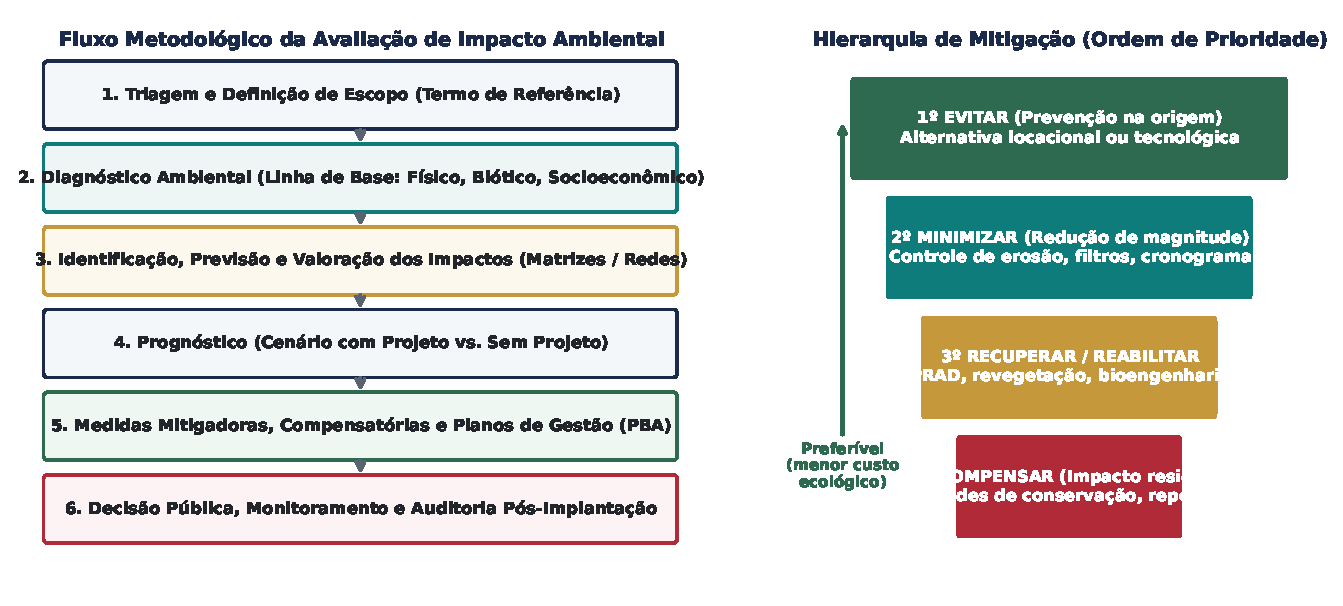
\includegraphics[width=0.95\textwidth]{figures/fig03_etapas_aia_mitigacao.pdf}
  \caption{Fluxo metodológico da Avaliação de Impacto Ambiental (a) e ordem de prioridade técnica da Hierarquia de Mitigação (b). Fonte: elaboração didática CHF662 com base em Sánchez (2013) e Brasil/MMA (2016).}
  \label{fig:aia_mitigacao}
\end{figure}

\subsection{Triagem e Definição de Escopo (Termo de Referência)}

A \textbf{triagem (\textit{screening})} abre o processo ao responder se o projeto requer EIA/RIMA completo, estudo ambiental simplificado ou dispensa de AIA. Essa decisão combina a tipologia da atividade (rodovias, parques eólicos, mineração ou barragens), o porte do empreendimento (área ocupada, potência instalada ou vazão captada) e a \textbf{sensibilidade ambiental do sítio}, avaliando a proximidade de Unidades de Conservação, terras indígenas, comunidades tradicionais, nascentes ou remanescentes de Caatinga conservada.

Confirmada a exigência de estudo ambiental, a \textbf{definição de escopo (\textit{scoping})} delimita os temas e processos que exigem investigação aprofundada, evitando relatórios extensos repletos de dados secundários desconexos e estudos omissos quanto aos riscos principais. O produto formal dessa etapa é o \textbf{Termo de Referência (TR)}, emitido pelo órgão ambiental competente (como o INEMA na Bahia ou o IBAMA na esfera federal) ou estruturado como proposta técnica pelo consultor para validação prévia.

Na prática profissional, uma proposta consistente de Termo de Referência encadeia cinco blocos integrados. O bloco inicial fixa a abrangência do estudo (EIA, RIMA e, quando houver risco químico ou tecnológico, Estudo de Análise de Risco) e exige levantamentos primários em campo articulados a bases oficiais recentes (IBGE, INEMA, ANA e universidades), com protocolos explícitos de amostragem. O bloco seguinte caracteriza o empreendimento por meio de cadastro técnico, histórico da área, mapa de localização em escala de detalhe (como $1{:}10.000$) inserido na bacia hidrográfica, mapa de restrições legais e descrição operacional de insumos, resíduos sólidos (ABNT NBR 10004 a 10007), efluentes, ruído e tráfego.

Em seguida, o TR especifica os parâmetros mínimos do diagnóstico na AID e na AII em escalas cartográficas compatíveis, usualmente $1{:}25.000$ para a AID e $1{:}50.000$ para a AII. Esse diagnóstico cobre geologia, geomorfologia, hidrografia e qualidade do ar no meio físico; inventários florísticos e faunísticos com curvas de suficiência amostral no meio biótico; e dinâmica demográfica, uso do solo, anuência do IPHAN para patrimônio arqueológico e levantamento específico de povos indígenas e comunidades quilombolas segundo registros da Fundação Cultural Palmares e do INCRA no meio socioeconômico. No bloco final, o documento define o método de valoração de impactos, os programas ambientais do PBA com cronograma e orçamento, as cartas temáticas sobre base planialtimétrica comum, as diretrizes de redação acessível do RIMA, as Anotações de Responsabilidade Técnica (ARTs) da equipe e os procedimentos de consulta pública.

\subsection{Diagnóstico Ambiental (Linha de Base) e Áreas de Influência}

O diagnóstico constrói a \textbf{linha de base (\textit{baseline})}, retratando de modo qualiquantitativo as condições do ambiente antes da intervenção. No \textbf{meio físico}, levantam-se clima, geologia, geomorfologia, solos, recursos hídricos superficiais e subterrâneos, qualidade do ar e ruído de fundo para aferir a suscetibilidade do substrato à erosão e às alterações hidrológicas. No \textbf{meio biótico}, inventariam-se fitofisionomias, flora (com atenção a espécies endêmicas e ameaçadas), fauna terrestre e aquática e corredores ecológicos. No \textbf{meio socioeconômico}, analisam-se demografia, uso e ocupação da terra, estrutura produtiva, serviços públicos, comunidades quilombolas, indígenas e de fundo de pasto e patrimônio cultural, revelando como os grupos locais dependem dos recursos afetados.

Para espacializar esses levantamentos, o diagnóstico delimita três escalas geográficas fundamentadas em processos físicos, ecológicos e territoriais reais, e nunca em círculos arbitrários traçados no mapa. A \textbf{Área Diretamente Afetada (ADA)} corresponde à superfície efetivamente ocupada pelas estruturas físicas do projeto, incluindo canteiros, estradas de acesso, jazidas e áreas de bota-fora, a exemplo da poligonal das bases de torres eólicas e das vias abertas na Caatinga. A \textbf{Área de Influência Direta (AID)} abrange o espaço submetido aos impactos primários de implantação e operação; no meio físico, acompanha os divisores topográficos da microbacia drenada pela ADA e a direção do escoamento superficial até o exutório afetado, enquanto nos meios biótico e socioeconômico acompanha manchas de ruído, dispersão de poeira, áreas de afugentamento de fauna e povoados lindeiros. A \textbf{Área de Influência Indireta (AII)} engloba o espaço atingido por desdobramentos secundários, como municípios receptores de tráfego pesado e arrecadação tributária ou a sub-bacia regional a jusante.

Traçar círculos concêntricos arbitrários ignora a direção natural da drenagem e deixa setores vulneráveis fora do monitoramento, erro contrastado com a delimitação hidrográfica correta na Figura~\ref{fig:areas_influencia}.

\begin{figure}[H]
  \centering
  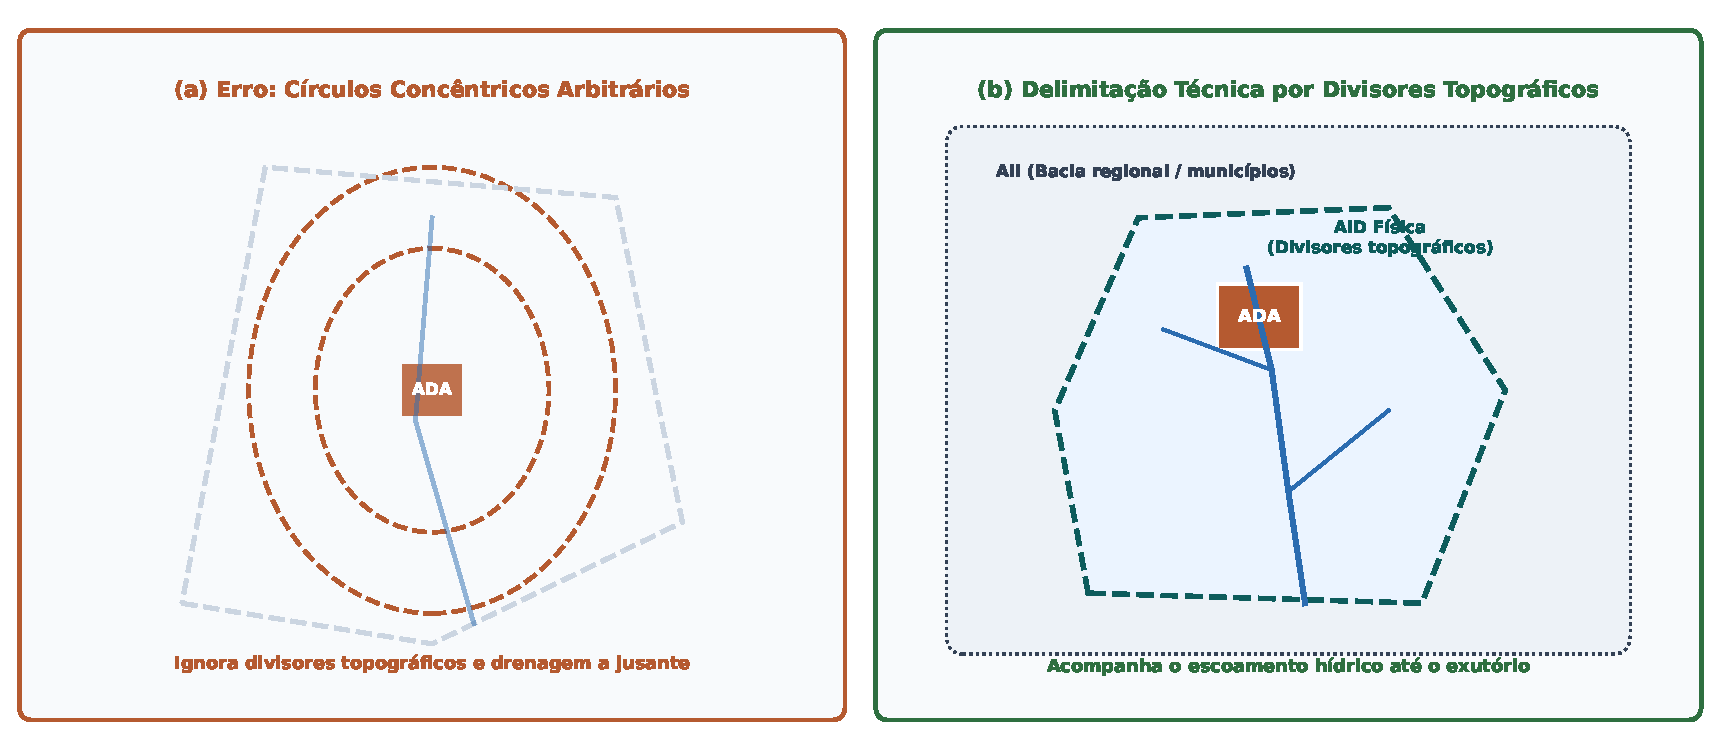
\includegraphics[width=0.96\textwidth]{figures/fig_cap05_areas_influencia.pdf}
  \caption{Delimitação técnica das Áreas de Influência (ADA, AID e AII) em bacia hidrográfica: (a) traçado circular arbitrário que ignora o escoamento e (b) delimitação física orientada pelos divisores topográficos e pela rede de drenagem a jusante da ADA. Fonte: elaboração didática CHF662 com base em Sánchez (2013).}
  \label{fig:areas_influencia}
\end{figure}

O Exemplo 5.1 quantifica a proporção espacial entre ADA, AID e AII em um empreendimento solar no Semiárido baiano.

\begin{boxExemplo}{5.1}{Delimitação Quantitativa de ADA, AID e AII em Parque Solar no Semiárido (Básico)}
  \passoEnunciado{Uma empresa propõe a instalação de uma usina solar fotovoltaica em área rural de transição semiárida na Bahia. O projeto prevê $45{,}0\text{ ha}$ ocupados pelos arranjos de painéis solares e $3{,}5\text{ ha}$ destinados à subestação, canteiro de obras e estradas internas de acesso. A microbacia hidrográfica que drena o empreendimento possui $620{,}0\text{ ha}$, e o município de inserção ocupa $48.500{,}0\text{ ha}$.}
  \passoDados{Área dos painéis $= 45{,}0\text{ ha}$; áreas de apoio e acessos $= 3{,}5\text{ ha}$; área da microbacia (AID do meio físico) $= 620{,}0\text{ ha}$; área do município (AII socioeconômica) $= 48.500{,}0\text{ ha}$.}
  \passoPedido{Calcular a Área Diretamente Afetada (ADA) total, determinar o percentual que a ADA representa em relação à AID e à AII, e justificar por que a AID do meio físico deve acompanhar os divisores da microbacia.}
  \passoMetodo{Soma das superfícies de intervenção direta para obtenção da ADA e cálculo das razões percentuais ($\text{ADA}/\text{AID} \times 100\%$ e $\text{ADA}/\text{AII} \times 100\%$), segundo os critérios espaciais de Sánchez (2013).}
  \passoContas{%
    Somando as superfícies de supressão e ocupação direta, obtém-se a ADA total e suas proporções nas áreas de influência:
    \begin{align*}
      \text{ADA} &= 45{,}0 + 3{,}5 = 48{,}5\text{ ha} \\
      \frac{\text{ADA}}{\text{AID}} \times 100\% &= \frac{48{,}5}{620{,}0} \times 100\% \approx 7{,}82\% \\
      \frac{\text{ADA}}{\text{AII}} \times 100\% &= \frac{48{,}5}{48.500{,}0} \times 100\% = 0{,}10\%.
    \end{align*}
    Quanto ao critério físico, o escoamento superficial, o carreamento de sedimentos e eventuais vazamentos de transformadores seguem a gravidade e os divisores topográficos. Um círculo fixo de $1\text{ km}$ incluiria trechos de bacias vizinhas sem conexão hídrica com o parque e deixaria de fora o exutório a jusante que receberá os sedimentos.}
  \passoResposta{$\text{ADA} = 48{,}5\text{ ha}$, correspondendo a $7{,}82\%$ da AID (microbacia) e $0{,}10\%$ da AII (município). A AID física deve coincidir com a microbacia porque os fluxos hidrossedimentológicos seguem a drenagem natural.}
  \passoVerificacao{A hierarquia espacial $\text{ADA} < \text{AID} < \text{AII}$ ($48{,}5 < 620{,}0 < 48.500{,}0\text{ ha}$) é coerente. Embora $0{,}10\%$ do município pareça pequeno na escala da AII, ocupar $7{,}82\%$ da microbacia local com superfícies compactadas altera o pico de escoamento superficial se faltarem drenagem e proteção do solo.}
\end{boxExemplo}

\subsection{Identificação, Previsão e Valoração de Impactos}

Nesta etapa, cruzam-se as ações do projeto (planejamento, implantação, operação e desativação) com os fatores ambientais descritos na linha de base. Cada impacto é caracterizado quanto à \textbf{natureza} (adverso ou benéfico), \textbf{incidência} (direto ou indireto), \textbf{abrangência} (local, regional ou estratégica), \textbf{temporalidade} (imediato, médio ou longo prazo), \textbf{duração} (temporário, permanente ou cíclico), \textbf{reversibilidade} (reversível ou irreversível) e \textbf{cumulatividade ou sinergia} com outros empreendimentos da bacia.

Quatro famílias metodológicas sustentam essa identificação e valoração conforme a complexidade do projeto. As \textbf{listagens de controle (\textit{checklists})} reúnem fatores ambientais e impactos potenciais por tipologia de obra em formato simples, descritivo ou escalar, oferecendo rapidez e padronização na triagem e no escopo, ainda que sejam estáticas e tenham dificuldade para explicitar encadeamentos indiretos. As \textbf{matrizes de interação}, com destaque para a Matriz de Leopold (Leopold et al., 1971) e suas versões ponderadas, cruzam em tabela bidimensional as ações do empreendimento (colunas) com os fatores ambientais (linhas), avaliando cada interação por sinal, magnitude e importância para hierarquizar prioridades.

Para rastrear cadeias causais complexas, empregam-se as \textbf{redes de interação (\textit{networks})}, estruturadas como grafos causa-efeito que encadeiam um impacto primário (direto) aos impactos secundários e terciários (indiretos). No Semiárido, a abertura de uma estrada sem sistema de drenagem desencadeia compactação e exposição do solo com concentração do escoamento superficial (1ª ordem), que evolui para sulcos erosivos, ravinas e carreamento de sedimentos ao riacho (2ª ordem) até assorear o açude comunitário e reduzir a oferta hídrica na estiagem (3ª ordem), encadeamento esquematizado na Figura~\ref{fig:rede_interacao}.

\begin{figure}[H]
  \centering
  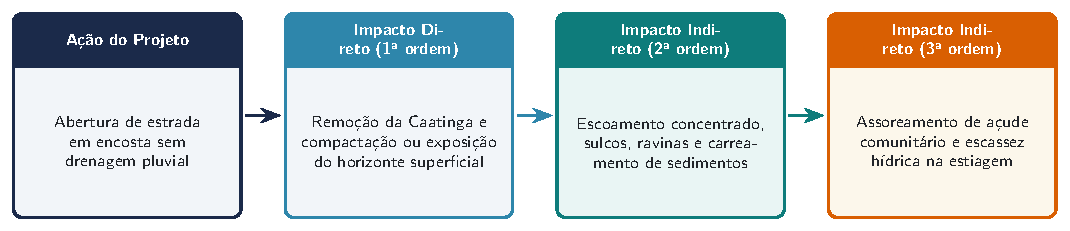
\includegraphics[width=0.95\textwidth]{figures/fig_cap05_rede_interacao.pdf}
  \caption{Rede de interação em cascata a partir da abertura de estrada sem drenagem, conectando a compactação inicial (1ª ordem) ao ravinamento (2ª ordem) e ao assoreamento de açudes a jusante (3ª ordem). Fonte: elaboração didática CHF662.}
  \label{fig:rede_interacao}
\end{figure}

Em campo, a transição da compactação inicial para o escoamento concentrado torna-se visível assim que as primeiras chuvas intensas incidem sobre a faixa exposta da via sem caixas secas ou saídas d'água, abrindo sulcos laterais que conduzem sedimentos para as drenagens próximas (Figura~\ref{fig:foto_estrada_sulco}).

\begin{figure}[H]
  \centering
  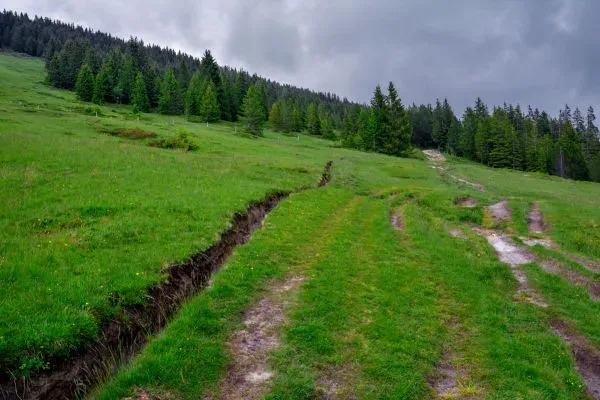
\includegraphics[width=0.68\textwidth]{figures/foto_estrada_sulco_erosivo.jpg}
  \caption{Registro de campo de escoamento concentrado e formação de sulco erosivo lateral em acesso rural sem drenagem pluvial. Fonte: acervo didático CHF662.}
  \label{fig:foto_estrada_sulco}
\end{figure}

Na quarta família metodológica, a \textbf{sobreposição de cartas (\textit{overlay}) e Sistemas de Informação Geográfica (SIG)}, derivada do método de Ian McHarg (1969), cruza camadas georreferenciadas (declividade, solos, hidrografia, APPs, remanescentes florestais e áreas urbanas) por álgebra de mapas. Essa abordagem explicita a distribuição espacial exata dos conflitos e subsidia a comparação de alternativas locacionais, dependendo da qualidade e da escala da base cartográfica adotada, tema aprofundado no Capítulo 6. A tabela a seguir sintetiza a escolha prática entre os quatro métodos.

\begin{center}
\renewcommand{\arraystretch}{1.20}
\small
\begin{tabularx}{\textwidth}{@{}p{2.7cm} >{\raggedright\arraybackslash}X >{\raggedright\arraybackslash}X p{2.7cm}@{}}
  \toprule
  \rowcolor{uefsNavy}
  \textcolor{white}{\bfseries Método} & \textcolor{white}{\bfseries Principal vantagem} & \textcolor{white}{\bfseries Principal limitação} & \textcolor{white}{\bfseries Uso ideal} \\
  \midrule
  \textbf{Checklists} & Rapidez e padronização inicial. & Estrutura estática, sem cadeias causais. & Triagem e escopo. \\
  \rowcolor{bgGray}
  \textbf{Matriz de Leopold} & Liga ações a fatores e prioriza ações críticas. & Pouca clareza para efeitos indiretos. & Síntese de EIAs e PCAs. \\
  \textbf{Redes de Interação} & Evidencia impactos indiretos e cumulativos. & Visualmente complexa em grandes projetos. & Bacias, erosão e hidrologia. \\
  \rowcolor{bgGray}
  \textbf{Sobreposição / SIG} & Localiza conflitos e compara traçados. & Depende da escala e qualidade dos mapas. & Traçados e zoneamentos. \\
  \bottomrule
\end{tabularx}
\end{center}

\subsection{Matriz de Leopold Ponderada: Magnitude, Importância e Balanço}

Na adaptação ponderada da Matriz de Leopold (Leopold et al., 1971), cada célula $(i, j)$ com interação efetiva entre o \textbf{fator ambiental $i$} (linha) e a \textbf{ação $j$} (coluna) recebe três parâmetros. O \textbf{sinal ($s_{ij} \in \{-1, +1\}$)} assume $-1$ para impacto adverso e $+1$ para impacto benéfico, registrando-se $0$ quando a interação é inexistente. A \textbf{magnitude ($M_{ij} \in \{1, \dots, 10\}$)} mede a intensidade e extensão física da alteração sobre o fator, enquanto a \textbf{importância ($I_{ij} \in \{1, \dots, 10\}$)} expressa a relevância ecológica, funcional, social ou legal do receptor atingido, atingindo notas máximas em nascentes, espécies ameaçadas ou comunidades tradicionais.

\begin{boxFormula}[Equações da Matriz de Leopold Ponderada]
\begin{align*}
  P_{ij} &= s_{ij} \cdot \left(M_{ij} \times I_{ij}\right), \qquad P_{ij} \in [-100, +100] \\[4pt]
  T_j &= \sum_{i=1}^{m} P_{ij} \qquad \text{(total da coluna } j \text{ sobre os } m \text{ fatores)} \\[4pt]
  F_i &= \sum_{j=1}^{n} P_{ij} \qquad \text{(total da linha } i \text{ sob as } n \text{ ações)} \\[4pt]
  B &= \sum_{i=1}^{m}\sum_{j=1}^{n} P_{ij} = \sum_{j=1}^{n} T_j = \sum_{i=1}^{m} F_i \\[4pt]
  \Sigma^{-} &= \sum_{P_{ij}<0} P_{ij}, \qquad \Sigma^{+} = \sum_{P_{ij}>0} P_{ij}
\end{align*}
Nessas equações, $P_{ij}$ é a pontuação celular, $T_j$ mede o saldo da ação $j$, $F_i$ acumula a pressão sobre o fator $i$, $B$ é o balanço líquido global, $\Sigma^{-}$ reúne a carga adversa total e $\Sigma^{+}$ soma a carga benéfica total.
\end{boxFormula}

Para acompanhar o cálculo em escala reduzida, considere uma mini-matriz com duas ações ($A_1$: supressão vegetal em encosta; $A_2$: contratação de mão de obra local) e dois fatores ($F_1$: solo e suscetibilidade erosiva; $F_2$: renda familiar). Na célula $(F_1, A_1)$, a supressão gera dano severo ($s=-1$, $M=8$, $I=9$), resultando em $P_{11} = -72$, enquanto em $(F_2, A_1)$ o pagamento temporário pela limpeza produz efeito positivo discreto ($s=+1$, $M=2$, $I=3$), com $P_{21} = +6$. A ação $A_2$ não altera fisicamente o solo ($P_{12} = 0$), mas eleva a renda local ($s=+1$, $M=6$, $I=7$), gerando $P_{22} = +42$. Somando colunas e linhas, tem-se $T_1 = -66$, $T_2 = +42$, $F_1 = -72$, $F_2 = +48$, carga adversa $\Sigma^{-} = -72$, carga benéfica $\Sigma^{+} = +48$ e balanço $B = -24$. A estrutura operacional dessa matriz em planilha eletrônica está representada na Figura~\ref{fig:matriz_leopold_excel}.

\begin{figure}[H]
  \centering
  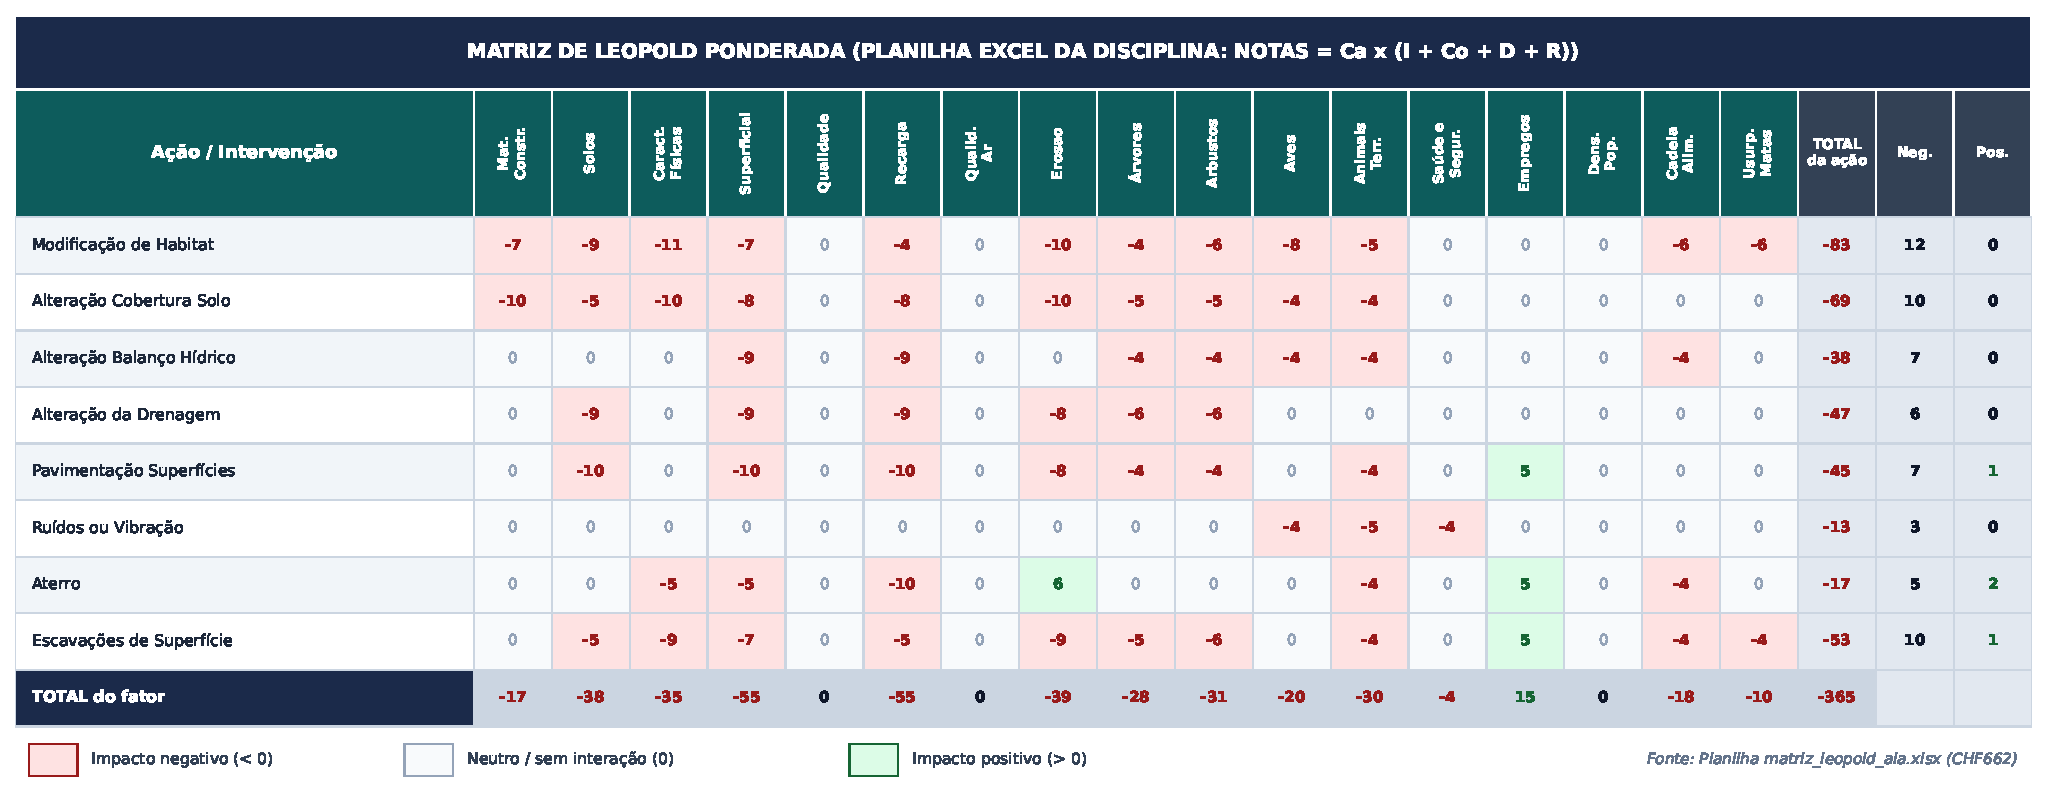
\includegraphics[width=0.98\textwidth]{figures/fig_cap05_matriz_leopold_excel.pdf}
  \caption{Matriz de Leopold Ponderada na planilha eletrônica da disciplina, destacando impactos adversos em vermelho, benéficos em verde e os totais por ação e fator ambiental. Fonte: planilha didática \texttt{matriz\_leopold\_aia.xlsx} (CHF662).}
  \label{fig:matriz_leopold_excel}
\end{figure}

O Exemplo 5.2 aplica esse equacionamento completo à avaliação de um parque eólico na Caatinga baiana.

\begin{boxExemplo}{5.2}{Matriz de Leopold Ponderada em Parque Eólico na Caatinga (Básico e Intermediário)}
  \passoEnunciado{Durante a AIA de um parque eólico no Semiárido baiano, a equipe técnica estruturou uma matriz cruzando três ações ($A_1$: supressão vegetal e abertura de acessos; $A_2$: escavação e concretagem das fundações das torres; $A_3$: operação dos aerogeradores e contratação de serviços locais) com quatro fatores ambientais ($F_1$: solo e processos erosivos; $F_2$: fauna e avifauna; $F_3$: qualidade da água superficial; $F_4$: emprego e renda local).}
  \passoDados{Avaliações $(s, M, I)$ atribuídas após vistorias de campo e linha de base: em $F_1$ (Solo/Erosão), $A_1 = (-, 8, 9)$, $A_2 = (-, 6, 8)$ e $A_3 = 0$; em $F_2$ (Fauna/Avifauna), $A_1 = (-, 7, 8)$, $A_2 = (-, 3, 5)$ e $A_3 = (-, 5, 9)$; em $F_3$ (Qualidade da água), $A_1 = (-, 5, 7)$, $A_2 = (-, 4, 7)$ e $A_3 = 0$; em $F_4$ (Emprego/Renda), $A_1 = (+, 3, 5)$, $A_2 = (+, 4, 5)$ e $A_3 = (+, 7, 8)$.}
  \passoPedido{Calcular todas as pontuações celulares $P_{ij}$, os totais por ação ($T_j$), os totais por fator ($F_i$), a carga adversa ($\Sigma^{-}$), a carga benéfica ($\Sigma^{+}$) e o balanço líquido ($B$), identificando a ação mais crítica e o fator mais impactado.}
  \passoMetodo{Aplicação das equações da Matriz de Leopold Ponderada ($P_{ij} = s_{ij} \cdot M_{ij} \cdot I_{ij}$), com verificação cruzada pela identidade $\sum T_j = \sum F_i = B$.}
  \passoContas{%
    Calculando cada célula por linha: em $F_1$, $P_{11} = -72$, $P_{12} = -48$ e $P_{13} = 0$; em $F_2$, $P_{21} = -56$, $P_{22} = -15$ e $P_{23} = -45$; em $F_3$, $P_{31} = -35$, $P_{32} = -28$ e $P_{33} = 0$; e em $F_4$, $P_{41} = +15$, $P_{42} = +20$ e $P_{43} = +56$. Os valores consolidam-se na matriz a seguir:
    \begin{center}
    \renewcommand{\arraystretch}{1.15}
    \small
    \begin{tabularx}{0.96\linewidth}{@{}X r r r r@{}}
      \toprule
      \textbf{Fator Ambiental} & \textbf{$A_1$ (Acessos)} & \textbf{$A_2$ (Fundações)} & \textbf{$A_3$ (Operação)} & \textbf{Total $F_i$} \\
      \midrule
      $F_1$, Solo / Erosão & $-72$ & $-48$ & $0$ & $\mathbf{-120}$ \\
      $F_2$, Fauna / Avifauna & $-56$ & $-15$ & $-45$ & $\mathbf{-116}$ \\
      $F_3$, Qualidade da água & $-35$ & $-28$ & $0$ & $\mathbf{-63}$ \\
      $F_4$, Emprego / Renda & $+15$ & $+20$ & $+56$ & $\mathbf{+91}$ \\
      \midrule
      \textbf{Total da Ação ($T_j$)} & $\mathbf{-148}$ & $\mathbf{-71}$ & $\mathbf{+11}$ & $\mathbf{B = -208}$ \\
      \bottomrule
    \end{tabularx}
    \end{center}
    Conferindo as somas marginais e separando as cargas adversa e benéfica:
    \begin{align*}
      \sum F_i &= (-120) + (-116) + (-63) + 91 = -208, \\
      \sum T_j &= (-148) + (-71) + 11 = -208, \\
      \Sigma^{-} &= -72 - 48 - 56 - 15 - 45 - 35 - 28 = -299, \\
      \Sigma^{+} &= +15 + 20 + 56 = +91.
    \end{align*}}
  \passoResposta{A ação mais impactante negativamente é $A_1$ (supressão e acessos, $T_1 = -148$) e o fator mais vulnerável é $F_1$ (solo/erosão, $F_1 = -120$), seguido de $F_2$ (fauna/avifauna, $F_2 = -116$). A carga adversa vale $\Sigma^{-} = -299$, a benéfica vale $\Sigma^{+} = +91$ e o balanço líquido fecha em $B = -208$.}
  \passoVerificacao{A igualdade $\sum F_i = \sum T_j = \Sigma^{-} + \Sigma^{+} = -208$ confirma a exatidão aritmética. Mesmo com $T_3 = +11$ na operação, a célula $P_{23} = -45$ (colisão de avifauna, com importância $I = 9$) exige monitoramento e desligamento preventivo para espécies como a arara-azul-de-lear na região de Canudos, jamais sendo anulada pelos $+56$ pontos de renda.}
\end{boxExemplo}

A interpretação isolada do saldo líquido $B$ costuma induzir erros graves na tomada de decisão, conforme detalhado no alerta a seguir.

\begin{boxErro}[Erro 2: Somar Benefícios Econômicos com Danos Ecológicos na Matriz]
  \textbf{Equívoco frequente:} Concluir que um empreendimento é ambientalmente viável porque a soma algébrica $B = \Sigma^{+} + \Sigma^{-}$ ficou positiva ou próxima de zero (por exemplo, $+80$ em arrecadação contra $-75$ em destruição de nascente).\par
  \textbf{Correção técnica:} A pontuação da Matriz de Leopold é semiquantitativa e reúne dimensões incomensuráveis. Empregos temporários não evitam o assoreamento de mananciais nem compensam a extinção local de fauna. Por isso, deve-se reportar $\Sigma^{-}$ e $\Sigma^{+}$ separadamente, destacando toda célula adversa de alta importância ($I \ge 8$) ou irreversível para vinculá-la a medidas concretas de mitigação.
\end{boxErro}

\subsection{Prognóstico Ambiental e Efeitos Cumulativos}

O prognóstico projeta a evolução futura da qualidade ambiental por meio de dois cenários comparativos obrigatórios com o mesmo horizonte temporal. O \textbf{cenário sem projeto (alternativa zero)} retrata a trajetória provável da bacia na ausência da obra, incorporando tendências já em curso como expansão urbana, sobrepastejo, variações climáticas ou regeneração natural. O \textbf{cenário com projeto} projeta a trajetória com o empreendimento em dois estágios: primeiro sem medidas mitigadoras, para dimensionar o risco potencial, e em seguida com os controles propostos, revelando o impacto residual. O impacto real atribuível ao projeto corresponde à diferença dinâmica entre a trajetória futura com o projeto e a trajetória futura sem o projeto.

Essa projeção deve considerar também os \textbf{impactos cumulativos}, que emergem quando pressões de diferentes empreendimentos convergem sobre o mesmo receptor. Estradas de parques eólicos vizinhos podem direcionar enxurradas para o mesmo riacho, enquanto captações distintas afetam a disponibilidade hídrica do mesmo trecho fluvial, exigindo definir explicitamente o receptor, a área de acumulação e o período analisado. O Exemplo 5.3 mostra como comparar alternativas locacionais no prognóstico por meio de critérios ponderados.

\begin{boxExemplo}{5.3}{Prognóstico e Seleção Multicritério de Alternativas Locacionais (Intermediário)}
  \passoEnunciado{No estudo de duplicação de uma rodovia estadual na Bahia, o EIA comparou duas alternativas locacionais diante do cenário sem projeto: o \textbf{Traçado A} (mais curto, atravessando uma APP de nascente e um fragmento contínuo de Caatinga) e o \textbf{Traçado B} ($1{,}2\text{ km}$ mais extenso, contornando a APP por áreas já antropizadas de pastagem).}
  \passoDados{Quatro critérios ponderados (soma dos pesos $= 1{,}00$) em escala de \textbf{severidade adversa} de $0$ (nenhum dano) a $10$ (dano máximo): $C_1$, supressão de APP e vegetação nativa ($w_1 = 0{,}35$; A $= 9$, B $= 3$); $C_2$, risco erosivo e assoreamento ($w_2 = 0{,}30$; A $= 8$, B $= 4$); $C_3$, fragmentação e atropelamento de fauna ($w_3 = 0{,}20$; A $= 8$, B $= 4$); $C_4$, custo e extensão adicional ($w_4 = 0{,}15$; A $= 4$, B $= 7$).}
  \passoPedido{Calcular o Índice de Impacto Adverso Ponderado ($I_{\text{adv}}$) de cada alternativa, determinar a redução percentual do índice ao optar pelo melhor traçado e identificar o degrau da Hierarquia de Mitigação correspondente.}
  \passoMetodo{Cálculo da média ponderada $I_{\text{adv}} = \sum_{k=1}^{4} w_k \cdot C_k$ e da variação relativa $(I_A - I_B)/I_A \times 100\%$.}
  \passoContas{%
    Os pesos somam $0{,}35 + 0{,}30 + 0{,}20 + 0{,}15 = 1{,}00$. Calculando os índices ponderados e a redução relativa de severidade:
    \begin{align*}
      I_A &= (0{,}35 \times 9) + (0{,}30 \times 8) + (0{,}20 \times 8) + (0{,}15 \times 4) \\
          &= 3{,}15 + 2{,}40 + 1{,}60 + 0{,}60 = 7{,}75 \\
      I_B &= (0{,}35 \times 3) + (0{,}30 \times 4) + (0{,}20 \times 4) + (0{,}15 \times 7) \\
          &= 1{,}05 + 1{,}20 + 0{,}80 + 1{,}05 = 4{,}10 \\
      \text{Redução} &= \frac{7{,}75 - 4{,}10}{7{,}75} \times 100\% = \frac{3{,}65}{7{,}75} \times 100\% \approx 47{,}10\%.
    \end{align*}}
  \passoResposta{O Traçado B é superior ($I_B = 4{,}10$ contra $I_A = 7{,}75$), reduzindo em $47{,}10\%$ a severidade adversa global. Essa escolha representa o 1º degrau da Hierarquia de Mitigação (\textbf{Evitar}), por alternativa locacional.}
  \passoVerificacao{Como a escala mede severidade adversa, o menor valor indica melhor desempenho. Apesar do maior custo inicial no critério $C_4$ ($7$ contra $4$), o Traçado B evita intervenções em APP, obras emergenciais contra erosão e passivos de compensação.}
\end{boxExemplo}

\subsection{Hierarquia de Mitigação, Medidas Mitigadoras e Compensatórias}

Diante de impactos adversos previstos, a tomada de decisão obedece a uma ordem estrita de prioridade técnica conhecida como \textbf{Hierarquia de Mitigação}, representada no Painel (b) da Figura~\ref{fig:aia_mitigacao}. No \textbf{1º degrau, Evitar (prevenção na origem)}, ajustam-se localização, traçado, cronograma ou tecnologia para impedir que o impacto ocorra, sendo o nível de maior eficácia ecológica. Quando a prevenção integral é inviável, aplica-se o \textbf{2º degrau, Minimizar}, utilizando controles de engenharia e manejo (como bacias de contenção de sedimentos, supressão seletiva e controle de poeira) para abater magnitude, duração ou extensão do dano.

Nas áreas afetadas temporariamente durante a obra, como canteiros, taludes de corte e áreas de empréstimo, atua-se no \textbf{3º degrau, Recuperar ou Reabilitar (\textit{in situ})}, restabelecendo as funções do solo, da drenagem e da cobertura vegetal mediante Plano de Recuperação de Áreas Degradadas (PRAD) e bioengenharia. Somente para o dano inevitável que persiste após esses três degraus, denominado \textbf{impacto residual}, recorre-se ao \textbf{4º degrau, Compensar}, por meio de apoio a Unidades de Conservação (art. 36 da Lei nº 9.985/2000, SNUC), reposição florestal equivalente ou superior e programas comunitários. De modo paralelo, impactos benéficos recebem \textbf{medidas potencializadoras}, como capacitação profissional prévia para ampliar a contratação de moradores locais.

O Exemplo 5.4 demonstra o abatimento sequencial (em cascata) ao longo dos quatro degraus da Hierarquia de Mitigação.

\begin{boxExemplo}{5.4}{Aplicação Sequencial da Hierarquia de Mitigação em Loteamento Periurbano (Intermediário e Avançado)}
  \passoEnunciado{O anteprojeto de um loteamento periurbano previa a supressão de $12{,}0\text{ ha}$ de vegetação nativa e um aporte de $480{,}0\text{ t/ano}$ de sedimentos para um riacho a jusante. Após revisão técnica, aplicaram-se sequencialmente os quatro degraus da Hierarquia de Mitigação.}
  \passoDados{No degrau \textbf{Evitar}, a exclusão de quadras em encostas íngremes evita $45\%$ da supressão e $45\%$ do aporte de sedimentos. No degrau \textbf{Minimizar}, o corte seletivo poupa $1{,}6\text{ ha}$ e bacias de contenção retêm $60\%$ do sedimento restante. No degrau \textbf{Recuperar}, a bioengenharia recupera $2{,}0\text{ ha}$ temporários e retém $75\%$ do sedimento remanescente. No degrau \textbf{Compensar}, exige-se reposição na razão $2{:}1$ sobre a perda permanente residual.}
  \passoPedido{Calcular o saldo remanescente de vegetação afetada e de sedimentos em cada degrau, o abatimento percentual acumulado de sedimentos e a área de compensação ecológica no 4º degrau.}
  \passoMetodo{Abatimento em cascata sobre o saldo remanescente de cada etapa, evitando somar percentuais diretamente sobre a carga inicial.}
  \passoContas{%
    Para a trajetória da supressão vegetal (em $\text{ha}$) e do aporte de sedimentos (em $\text{t/ano}$), aplicam-se os abatimentos etapa a etapa:
    \begin{align*}
      \text{Vegetação após Evitar} &= 12{,}0 - (0{,}45 \times 12{,}0) = 12{,}0 - 5{,}4 = 6{,}6\text{ ha} \\
      \text{após Minimizar} &= 6{,}6 - 1{,}6 = 5{,}0\text{ ha} \\
      \text{após Recuperar (residual)} &= 5{,}0 - 2{,}0 = 3{,}0\text{ ha} \\
      \text{Área a Compensar (}2{:}1\text{)} &= 2 \times 3{,}0 = 6{,}0\text{ ha}
    \end{align*}
    \begin{align*}
      \text{Sedimentos após Evitar} &= 480{,}0 - (0{,}45 \times 480{,}0) = 264{,}0\text{ t/ano} \\
      \text{após Minimizar} &= 264{,}0 - (0{,}60 \times 264{,}0) = 105{,}6\text{ t/ano} \\
      \text{após Recuperar (residual)} &= 105{,}6 - (0{,}75 \times 105{,}6) = 26{,}4\text{ t/ano} \\
      \text{Abatimento acumulado} &= \frac{480{,}0 - 26{,}4}{480{,}0} \times 100\% = 94{,}50\%.
    \end{align*}}
  \passoResposta{O impacto residual permanente reduz-se a $3{,}0\text{ ha}$ de vegetação (exigindo $6{,}0\text{ ha}$ de compensação na razão $2{:}1$) e a $26{,}4\text{ t/ano}$ de sedimentos (abatimento total de $94{,}50\%$).}
  \passoVerificacao{Pelo produto em cascata, $480{,}0 \times 0{,}55 \times 0{,}40 \times 0{,}25 = 26{,}4\text{ t/ano}$. Sem seguir a hierarquia, tentar compensar os $12{,}0\text{ ha}$ iniciais exigiria $24{,}0\text{ ha}$ de reposição e manteria o riacho assoreado com $480\text{ t/ano}$ de sedimentos.}
\end{boxExemplo}

Propor compensação financeira antes de esgotar alternativas locacionais e medidas de engenharia viola diretamente a Hierarquia de Mitigação, como alerta o quadro a seguir.

\begin{boxErro}[Erro 3: Inverter a Hierarquia de Mitigação ao Priorizar a Compensação]
  \textbf{Equívoco frequente:} Propor diretamente compensação financeira ou plantio em outro município para suprimir uma APP ou fragmento florestal sem avaliar alternativas de traçado ou tecnologia que evitassem a perda.\par
  \textbf{Correção técnica:} A compensação ocupa o \textbf{4º e último degrau} da hierarquia, destinando-se exclusivamente ao impacto residual que permanece após esgotadas as etapas de evitar, minimizar e recuperar no local.
\end{boxErro}

\subsection{Plano Básico Ambiental (PBA) e Monitoramento Pós-Implantação}

Na etapa decisória, o órgão ambiental emite parecer técnico pelo deferimento com condicionantes ou pelo indeferimento das licenças (Licença Prévia, Licença de Instalação e Licença de Operação). Os compromissos assumidos no EIA convertem-se em projetos executivos detalhados no \textbf{Plano Básico Ambiental (PBA)}, que estrutura programas de controle de erosão, monitoramento da qualidade da água, resgate de fauna, educação ambiental e PRAD. Cada programa necessita de condição inicial documentada, meta verificável, frequência de amostragem e responsável técnico.

O \textbf{monitoramento pós-implantação} fecha o ciclo da AIA ao confrontar os indicadores medidos em operação com os valores da linha de base e interpretar desvios junto aos registros de chuva e manutenção. Caso um indicador ultrapasse o limite da condicionante ambiental, aciona-se a \textbf{gestão adaptativa} para corrigir imediatamente os dispositivos de controle em campo.

% ============================================================================
% ETAPA 4 — ESTUDO DE CASO AVANÇADO (EXEMPLO 5.5)
% ============================================================================
\etapa{4}{Aplicação Integrada: Auditoria de Monitoramento no PBA}

A verificação quantitativa de desempenho durante a obra exige descontar a condição natural registrada na linha de base antes de calcular a eficiência das medidas de controle, evitando subestimar ou superestimar o abatimento real obtido em campo, como demonstrado no Exemplo 5.5.

\begin{boxExemplo}{5.5}{Auditoria de Eficiência no Monitoramento Pós-Implantação do PBA (Avançado)}
  \passoEnunciado{Durante a construção de uma barragem de regularização hídrica no rio Jacuípe (Bahia), a linha de base registrou turbidez média de $18{,}0\text{ NTU}$ a jusante em estiagem. Na terraplenagem inicial sem controle, a turbidez subiu para $112{,}0\text{ NTU}$. Após a instalação de cortinas de siltagem e diques do PBA, o monitoramento mediu $33{,}0\text{ NTU}$. A condicionante da Licença de Instalação fixava limite máximo de $40{,}0\text{ NTU}$.}
  \passoDados{Linha de base $T_0 = 18{,}0\text{ NTU}$; turbidez sem mitigação $T_{\text{sem}} = 112{,}0\text{ NTU}$; turbidez com PBA $T_{\text{com}} = 33{,}0\text{ NTU}$; limite legal $T_{\max} = 40{,}0\text{ NTU}$.}
  \passoPedido{Calcular o acréscimo de turbidez atribuível à obra sem mitigação, o acréscimo residual após o PBA, a eficiência percentual de abatimento da carga antrópica e emitir parecer técnico sobre o atendimento à condicionante.}
  \passoMetodo{Cálculo da anomalia acima da linha de base ($\Delta T = T - T_0$) e da eficiência de abatimento incremental $E_f = \frac{\Delta T_{\text{sem}} - \Delta T_{\text{com}}}{\Delta T_{\text{sem}}} \times 100\%$.}
  \passoContas{%
    Descontando a turbidez natural $T_0$ da linha de base, calculam-se os acréscimos e a eficiência do PBA:
    \begin{align*}
      \Delta T_{\text{sem}} &= 112{,}0 - 18{,}0 = 94{,}0\text{ NTU} \\
      \Delta T_{\text{com}} &= 33{,}0 - 18{,}0 = 15{,}0\text{ NTU} \\
      \Delta T_{\text{abatida}} &= 94{,}0 - 15{,}0 = 79{,}0\text{ NTU} \\
      E_f &= \frac{79{,}0}{94{,}0} \times 100\% \approx 84{,}04\%.
    \end{align*}
    Como $33{,}0\text{ NTU} \le 40{,}0\text{ NTU}$, a condicionante da Licença de Instalação está atendida com folga de $7{,}0\text{ NTU}$.}
  \passoResposta{O acréscimo sem controle foi de $94{,}0\text{ NTU}$, reduzido para $15{,}0\text{ NTU}$ residuais com eficiência de abatimento de $84{,}04\%$. A condicionante de $40{,}0\text{ NTU}$ está atendida, mantendo-se o monitoramento contínuo na estação chuvosa.}
  \passoVerificacao{Descontar $T_0 = 18{,}0\text{ NTU}$ no denominador é indispensável porque o controle ambiental visa abater o acréscimo gerado pela obra sobre o fundo natural do rio; sem esse desconto, o cálculo subestimaria a eficiência real ($79/112 = 70{,}54\%$).}
\end{boxExemplo}

% ============================================================================
% ETAPA 5 — ERRO 4 E MATERIAIS AUDIOVISUAIS DE APOIO
% ============================================================================
\etapa{5}{Armadilha Conceitual e Materiais Audiovisuais de Apoio}

Mesmo quando um estudo adota equações corretas na matriz de impacto ou no monitoramento do PBA, uma delimitação espacial mal fundamentada compromete toda a amostragem dos meios físico, biótico e socioeconômico.

\begin{boxErro}[Erro 4: Delimitar ADA, AID e AII como Círculos Concêntricos Arbitrários]
  \textbf{Equívoco frequente:} Traçar raios fixos de $500\text{ m}$ (AID) e $5\text{ km}$ (AII) no mapa sem considerar divisores de bacia, direção dos ventos, rotas de fauna ou malha viária.\par
  \textbf{Correção técnica:} Processos ambientais propagam-se segundo fluxos físicos e sociais anisotrópicos. Um efluente lançado num riacho percorre quilômetros a jusante pelo talvegue, mas permanece ausente a $200\text{ m}$ além do divisor topográfico. Delimite a AID física pela microbacia drenada, a AID biótica pelos habitats conectados e a AII pela rede territorial e municipal afetada.
\end{boxErro}

Para consolidar o entendimento sobre degradação ambiental, papel preventivo da AIA e estruturação de EIA/RIMA, assista às videoaulas selecionadas na página da disciplina: \textit{O papel da Avaliação de Impacto Ambiental na gestão ambiental} (\url{https://www.youtube.com/watch?v=oDceh9hvPc8}), \textit{EIA-RIMA, Conceitos e Definições de Impactos Ambientais} (\url{https://www.youtube.com/watch?v=m8rg8SnhSfQ}) e \textit{Degradação Ambiental} (\url{https://www.youtube.com/watch?v=5EFxN7jGob8}), que articulam diagnóstico, prognóstico e medidas mitigadoras no licenciamento brasileiro.

% ============================================================================
% ETAPA 6 — EXERCÍCIOS DE FIXAÇÃO (15 EXERCÍCIOS: 5 BÁSICOS, 5 INTERM., 5 OBJ.)
% ============================================================================
\etapa{6}{Exercícios de Fixação}

\subsection*{Nível 1: Básico (Conceitos, Etapas e Cálculos Fundamentais)}

\begin{enumerate}[leftmargin=1.8em, itemsep=4pt]
  \item Explique, com base em Sánchez (2013), qual é o papel preventivo da Avaliação de Impacto Ambiental (AIA) e por que sua inserção tardia, após a definição do projeto de engenharia, compromete sua eficácia no planejamento ambiental.
  \espacoResolucao[2.0cm]

  \item Em uma matriz de interação ponderada adaptada de Leopold, uma atividade de terraplenagem apresentou três interações relevantes: solo e erosão $(-, M=7, I=8)$; qualidade do ar por poeira $(-, M=4, I=6)$; e contratação temporária de operadores locais $(+, M=6, I=5)$. Calcule a pontuação $P_{ij}$ de cada célula, a carga adversa ($\Sigma^{-}$), a carga benéfica ($\Sigma^{+}$) e o total $T_j$ dessa ação.
  \espacoResolucao[2.2cm]

  \item Diferencie claramente as etapas de \textbf{triagem (\textit{screening})} e \textbf{definição de escopo (\textit{scoping})}, indicando qual documento oficial formaliza o resultado da definição de escopo no licenciamento ambiental brasileiro.
  \espacoResolucao[2.0cm]

  \item Defina \textbf{ADA}, \textbf{AID} e \textbf{AII} e dê um exemplo concreto de cada uma para a implantação de um aterro sanitário regional no interior da Bahia.
  \espacoResolucao[2.1cm]

  \item Compare as quatro famílias de métodos de identificação de impactos (\textit{checklists}, Matriz de Leopold, redes de interação e sobreposição de cartas em SIG), indicando uma vantagem específica de cada método.
  \espacoResolucao[2.2cm]
\end{enumerate}

\subsection*{Nível 2: Intermediário (Aplicação Quantitativa e Análise Técnica)}

\begin{enumerate}[leftmargin=1.8em, itemsep=4pt, resume]
  \item Um empreendimento de extração de areia em planície fluvial foi avaliado por meio de uma matriz ponderada $3 \times 3$, com as ações $A_1$ (dragagem no leito), $A_2$ (abertura de pátio e estrada de acesso) e $A_3$ (comercialização e geração de empregos) e os fatores $F_1$ (estabilidade das margens e do leito), $F_2$ (turbidez e biota aquática) e $F_3$ (renda e arrecadação municipal):
  \begin{itemize}[leftmargin=1.4em, itemsep=1pt]
    \item $F_1$: $A_1=(-, 9, 9)$; $A_2=(-, 5, 7)$; $A_3=0$.
    \item $F_2$: $A_1=(-, 8, 8)$; $A_2=(-, 4, 6)$; $A_3=0$.
    \item $F_3$: $A_1=(+, 3, 4)$; $A_2=(+, 2, 4)$; $A_3=(+, 6, 6)$.
  \end{itemize}
  Calcule todas as células $P_{ij}$, os totais $T_j$ e $F_i$, $\Sigma^{-}$, $\Sigma^{+}$ e o balanço $B$. Identifique a ação mais degradadora e o fator mais crítico.
  \espacoResolucao[3.2cm]

  \item Um projeto agroindustrial previa inicialmente suprimir $20{,}0\text{ ha}$ de vegetação nativa. Aplicando a Hierarquia de Mitigação, a realocação do galpão evitou $35\%$ da supressão inicial; o ajuste das vias internas minimizou $20\%$ da área restante; e a restauração de áreas temporárias recuperou $2{,}4\text{ ha}$. Sabendo que o órgão licenciador determinou compensação na razão $3{:}1$ sobre o impacto permanente residual, calcule a área remanescente em cada degrau e a área total a ser compensada.
  \espacoResolucao[2.8cm]

  \item Na escolha tecnológica para uma Estação de Tratamento de Efluentes (ETE), duas opções ($E_1$ e $E_2$) foram avaliadas em escala de \textbf{desempenho ambiental positivo} ($0$ = péssimo; $10$ = excelente) sob quatro critérios ponderados: eficiência de remoção de carga orgânica ($w_1 = 0{,}35$: $E_1=6$, $E_2=9$), controle de odores ($w_2 = 0{,}30$: $E_1=5$, $E_2=8$), possibilidade de reúso agrícola no Semiárido ($w_3 = 0{,}20$: $E_1=7$, $E_2=8$) e menor custo de implantação ($w_4 = 0{,}15$: $E_1=9$, $E_2=6$). Calcule a nota ponderada de cada alternativa e justifique a escolha técnica.
  \espacoResolucao[2.6cm]

  \item Desenhe ou descreva textualmente uma \textbf{rede de interação} de três níveis (impacto primário $\to$ secundário $\to$ terciário) desencadeada pela abertura de vias de acesso sem drenagem em encosta declivosa da Caatinga, associando ao menos uma medida preventiva e uma medida corretiva do PBA para interromper a cascata.
  \espacoResolucao[2.4cm]

  \item No monitoramento do PBA de uma obra rodoviária, a linha de base de Sólidos Suspensos Totais (SST) em um riacho era de $25{,}0\text{ mg/L}$. Durante a escavação sem bacias de decantação, o valor atingiu $145{,}0\text{ mg/L}$. Após a implantação das bacias previstas no PBA, a concentração caiu para $43{,}0\text{ mg/L}$. Calcule o acréscimo sem controle, o acréscimo residual e a eficiência percentual de abatimento da carga antrópica.
  \espacoResolucao[2.4cm]
\end{enumerate}

\subsection*{Nível 3: Questões Objetivas de Fixação (A a E)}

\begin{enumerate}[leftmargin=1.8em, itemsep=5pt, resume]
  \item \textbf{[Autoral, CHF662]} No processo de Avaliação de Impacto Ambiental, o prognóstico compara o cenário com projeto ao cenário sem projeto (alternativa zero). Assinale a alternativa que interpreta corretamente o conceito de \textbf{cenário sem projeto}:
  \begin{alternativas}
    \item Representa a manutenção estática e imutável das condições atuais medidas na linha de base, sem qualquer variação futura.
    \item Projeta a evolução futura provável do ambiente na ausência do empreendimento, incorporando tendências climáticas, ecológicas e de uso da terra já em curso.
    \item Equivale ao cenário com projeto após a aplicação integral das medidas compensatórias previstas no PBA.
    \item É exigido apenas quando o empreendedor decide abandonar a obra antes da emissão da Licença Prévia.
    \item Dispensa a realização do diagnóstico ambiental da linha de base nos meios físico e biótico.
  \end{alternativas}
  \espacoResolucao[1.2cm]

  \item \textbf{[Autoral, CHF662]} Assinale a alternativa que apresenta na ordem correta, da maior para a menor prioridade técnica e ecológica, os degraus da \textbf{Hierarquia de Mitigação}:
  \begin{alternativas}
    \item Compensar $\to$ Recuperar $\to$ Minimizar $\to$ Evitar.
    \item Minimizar $\to$ Evitar $\to$ Compensar $\to$ Recuperar.
    \item Evitar $\to$ Recuperar $\to$ Minimizar $\to$ Compensar.
    \item Evitar $\to$ Minimizar $\to$ Recuperar $\to$ Compensar.
    \item Monitorar $\to$ Compensar $\to$ Evitar $\to$ Minimizar.
  \end{alternativas}
  \espacoResolucao[1.2cm]

  \item \textbf{[Autoral, CHF662]} Em uma Matriz de Leopold Ponderada ($P_{ij} = s_{ij} \cdot M_{ij} \cdot I_{ij}$), uma ação de instalação de canteiro de obras apresentou três células preenchidas: erosão laminar $(-, M=8, I=9)$, afugentamento de fauna $(-, M=6, I=7)$ e geração de empregos temporários $(+, M=5, I=4)$. Sobre o resultado dessa coluna, é correto afirmar que:
  \begin{alternativas}
    \item A pontuação líquida da ação é $T = -94$, com carga adversa $\Sigma^{-} = -114$, e os $+20$ pontos de emprego não eliminam a necessidade de controle erosivo.
    \item A pontuação líquida da ação é $T = -134$, pois todas as células devem ser somadas em módulo negativo.
    \item A pontuação líquida da ação é $T = -52$, obtida somando apenas magnitude e importância sem multiplicá-las.
    \item Como existem $+20$ pontos benéficos, o impacto de erosão laminar cai automaticamente de $-72$ para $-52$.
    \item A pontuação líquida da ação é $T = +114$, caracterizando a ação como ambientalmente neutra.
  \end{alternativas}
  \espacoResolucao[1.2cm]

  \item \textbf{[Autoral, CHF662]} Qual método de identificação e avaliação de impactos é o mais adequado para \textbf{explicitar visualmente o encadeamento entre impactos primários (diretos) e impactos secundários e terciários (indiretos)} em uma bacia hidrográfica?
  \begin{alternativas}
    \item Listagem de controle simples (\textit{checklist} binário).
    \item Rede de interação (grafo causa-efeito).
    \item Inventário financeiro de compensação ambiental.
    \item Formulário cadastral de triagem administrativa.
    \item Tabela de coordenadas geográficas da ADA.
  \end{alternativas}
  \espacoResolucao[1.2cm]

  \item \textbf{[Autoral, CHF662]} Em relação ao \textbf{Plano Básico Ambiental (PBA)} e ao monitoramento pós-implantação, assinale a afirmação correta:
  \begin{alternativas}
    \item O PBA substitui o diagnóstico da linha de base, sendo entregue antes mesmo da definição de escopo.
    \item O monitoramento pós-implantação tem caráter meramente decorativo, pois as previsões do EIA nunca apresentam incertezas.
    \item O PBA detalha operacionalmente os programas de mitigação, controle, recuperação e monitoramento, cujos indicadores são comparados à linha de base para permitir gestão adaptativa.
    \item O PBA aplica-se exclusivamente à compensação financeira prevista na Lei do SNUC, não contemplando controle de erosão nem qualidade da água.
    \item O monitoramento só deve iniciar após a desativação definitiva do empreendimento.
  \end{alternativas}
  \espacoResolucao[1.2cm]
\end{enumerate}

% ============================================================================
% ETAPA 7 — QUESTÕES DE PROVAS, ENADE E CONCURSOS AMBIENTAIS (3 AUTORAIS)
% ============================================================================
\etapa{7}{Questões no Estilo ENADE e Concursos Ambientais}

\begin{enumerate}[leftmargin=1.8em, itemsep=5pt, resume]
  \item \textbf{[Autoral, Estilo ENADE / Geografia]} A implantação de grandes empreendimentos energéticos e rodoviários no Semiárido brasileiro exige estudos ambientais rigorosos no âmbito da AIA. Considere as afirmações a seguir sobre o papel do geógrafo na AIA:
  \begin{enumerate}[label=\Roman*., leftmargin=2.0em, itemsep=2pt]
    \item A delimitação das áreas de influência (ADA, AID e AII) deve respeitar a dinâmica espacial específica de cada meio, como divisores de microbacias no meio físico e redes de mobilidade e serviços no meio socioeconômico, descartando raios circulares arbitrários.
    \item A sobreposição de cartas em SIG (inspirada no método de McHarg) permite integrar fragilidades do relevo, solos, APPs e uso da terra para subsidiar a escolha de alternativas locacionais que evitem impactos na origem.
    \item Na fase de prognóstico, o diagnóstico da linha de base torna-se dispensável porque a compensação ambiental corrige automaticamente todos os impactos residuais.
  \end{enumerate}
  É correto o que se afirma apenas em:
  \begin{alternativas}
    \item I.
    \item III.
    \item I e II.
    \item II e III.
    \item I, II e III.
  \end{alternativas}
  \espacoResolucao[1.2cm]

  \item \textbf{[Autoral, Estilo Concurso Analista Ambiental / IBAMA e INEMA]} Uma consultoria apresentou ao órgão ambiental um EIA de uma ferrovia cujo traçado original cortava um trecho de mata ciliar e uma nascente perene. No capítulo de mitigação, o estudo manteve o traçado original e propôs, como única medida, o pagamento de compensação financeira para criação de parque em outra região do Estado. À luz da teoria da AIA (Sánchez, 2013) e da Hierarquia de Mitigação, o parecer técnico do analista ambiental deve:
  \begin{alternativas}
    \item Aprovar integralmente a proposta, pois a compensação financeira ocupa o topo da Hierarquia de Mitigação.
    \item Exigir complementação do estudo com avaliação efetiva de alternativas locacionais (degrau \emph{Evitar}) e de medidas de engenharia para redução de danos (degrau \emph{Minimizar}), reservando a compensação estritamente a eventuais impactos residuais inevitáveis.
    \item Dispensar a etapa de monitoramento no PBA, já que o recurso financeiro foi depositado previamente.
    \item Substituir o EIA por uma listagem de controle simples, pois ferrovias não geram impactos indiretos.
    \item Aprovar a obra desde que a soma algébrica da Matriz de Leopold seja positiva devido à geração de empregos.
  \end{alternativas}
  \espacoResolucao[1.2cm]

  \item \textbf{[Autoral, Estilo Concurso Órgão Ambiental Estadual]} Associe corretamente cada instrumento ou etapa da AIA à sua função principal:
  \begin{center}
  \small
  \begin{tabularx}{0.96\linewidth}{@{}l X@{}}
    (1) Termo de Referência (TR) & (\quad) Execução operacional de programas de controle, recuperação e monitoramento na implantação/operação. \\
    (2) Diagnóstico (Linha de Base) & (\quad) Definição do escopo, conteúdo técnico mínimo e profundidade exigida nos estudos ambientais. \\
    (3) Matriz de Leopold & (\quad) Caracterização prévia dos meios físico, biótico e socioeconômico antes da intervenção. \\
    (4) Plano Básico Ambiental (PBA) & (\quad) Cruzamento sistemático entre ações do projeto e fatores ambientais por magnitude e importância. \\
  \end{tabularx}
  \end{center}
  A sequência numérica correta, de cima para baixo, é:
  \begin{alternativas}
    \item 4, 1, 2, 3.
    \item 1, 4, 3, 2.
    \item 4, 2, 1, 3.
    \item 3, 1, 2, 4.
    \item 2, 1, 4, 3.
  \end{alternativas}
  \espacoResolucao[1.2cm]
\end{enumerate}

\begin{boxDica}[Conexão com o Estudo Orientado EO4 e o Trabalho Prático Final]
  No \textbf{Estudo Orientado EO4} (Semana 5), ao analisar o texto de Sánchez (2013, cap. 7) e o guia do MMA (2016), concentre sua argumentação na AIA como processo preventivo de decisão, na escolha justificada de métodos (matriz ponderada, rede de interação e SIG) e na aplicação rigorosa da Hierarquia de Mitigação. No \textbf{Trabalho Prático Final}, a mesma sequência entre linha de base, valoração de impactos e hierarquia de intervenção estruturará o plano de manejo da área de estudo.
\end{boxDica}

% ============================================================================
% ETAPA 8 — GABARITO COMENTADO (PÁGINA SEPARADA — TODOS OS 18 EXERCÍCIOS)
% ============================================================================
\clearpage
\etapa{8}{Gabarito Comentado e Resoluções Passo a Passo}

\begin{boxGabarito}[Resoluções dos Exercícios 1 a 10 (Básicos e Intermediários)]
  \begin{enumerate}[leftmargin=1.8em, itemsep=4pt]
    \item \textbf{Papel preventivo da AIA:} a AIA antecipa consequências físicas, bióticas e socioeconômicas \emph{antes} da decisão de autorizar um empreendimento, orientando alternativas locacionais, tecnológicas e a alternativa zero. Quando inserida tardiamente (com traçado e engenharia já fechados), resta apenas remediar danos ou compensar perdas que poderiam ter sido evitadas na origem, desvirtuando o planejamento ambiental.

    \item \textbf{Cálculo de 3 células da Matriz de Leopold:}
    \begin{itemize}[leftmargin=1.4em, itemsep=1pt]
      \item Solo e erosão: $P_1 = -1 \times (7 \times 8) = -56$.
      \item Qualidade do ar: $P_2 = -1 \times (4 \times 6) = -24$.
      \item Contratação local: $P_3 = +1 \times (6 \times 5) = +30$.
      \item Carga adversa: $\Sigma^{-} = -56 + (-24) = -80$; carga benéfica: $\Sigma^{+} = +30$; total da ação: $T = -80 + 30 = -50$.
    \end{itemize}

    \item \textbf{Triagem versus Definição de Escopo:} a \emph{triagem} (\textit{screening}) decide \emph{se} o projeto precisa de AIA e qual o grau de complexidade do estudo (EIA/RIMA, estudo simplificado ou dispensa). A \emph{definição de escopo} (\textit{scoping}) estabelece \emph{quais} temas, métodos, áreas e impactos críticos devem ser aprofundados. Seu produto oficial é o \textbf{Termo de Referência (TR)}.

    \item \textbf{ADA, AID e AII para um aterro sanitário:}
    \begin{itemize}[leftmargin=1.4em, itemsep=1pt]
      \item \textbf{ADA:} poligonal das células de resíduos, lagoas de chorume, drenagem, balança e vias internas.
      \item \textbf{AID:} microbacia a jusante passível de sofrer alterações hídricas caso ocorra vazamento, área de dispersão de odores e ruído e propriedades vizinhas diretamente expostas.
      \item \textbf{AII:} municípios consorciados que enviam resíduos ao aterro e a sub-bacia hidrográfica regional.
    \end{itemize}

    \item \textbf{Vantagem específica de cada método:} \textit{checklists} oferecem rapidez e padronização inicial; a Matriz de Leopold estabelece vínculo explícito entre cada ação e cada fator com priorização por magnitude e importância; as redes de interação rastreiam impactos indiretos (2ª e 3ª ordens) e efeitos em cascata; e a sobreposição de cartas em SIG explicita os conflitos espaciais para subsidiar alternativas locacionais.

    \item \textbf{Matriz $3 \times 3$ completa (extração de areia):}
    \begin{itemize}[leftmargin=1.4em, itemsep=1pt]
      \item Linha $F_1$ (Margens/leito): $P_{11} = -(9 \times 9) = -81$; $P_{12} = -(5 \times 7) = -35$; $P_{13} = 0 \implies F_1 = -81 - 35 = -116$.
      \item Linha $F_2$ (Turbidez/biota): $P_{21} = -(8 \times 8) = -64$; $P_{22} = -(4 \times 6) = -24$; $P_{23} = 0 \implies F_2 = -64 - 24 = -88$.
      \item Linha $F_3$ (Renda/arrecadação): $P_{31} = +(3 \times 4) = +12$; $P_{32} = +(2 \times 4) = +8$; $P_{33} = +(6 \times 6) = +36 \implies F_3 = +56$.
      \item Somas das colunas: $T_1 = -81 - 64 + 12 = -133$; $T_2 = -35 - 24 + 8 = -51$; $T_3 = 0 + 0 + 36 = +36$.
      \item Cargas e balanço: $\Sigma^{-} = -81 - 35 - 64 - 24 = -204$; $\Sigma^{+} = +12 + 8 + 36 = +56$; $B = -204 + 56 = -148$ (confirmação: $F_1+F_2+F_3 = -116 - 88 + 56 = -148$ e $T_1+T_2+T_3 = -133 - 51 + 36 = -148$).
      \item \textbf{Conclusão:} a ação mais degradadora é $A_1$ (dragagem, $T_1 = -133$) e o fator mais crítico é $F_1$ (estabilidade de margens e leito, $F_1 = -116$).
    \end{itemize}

    \item \textbf{Hierarquia de Mitigação (projeto agroindustrial):}
    \begin{itemize}[leftmargin=1.4em, itemsep=1pt]
      \item Inicial: $20{,}0\text{ ha}$.
      \item 1º Evitar ($35\%$): evita $0{,}35 \times 20{,}0 = 7{,}0\text{ ha} \implies$ restam $20{,}0 - 7{,}0 = 13{,}0\text{ ha}$.
      \item 2º Minimizar ($20\%$ do restante): reduz $0{,}20 \times 13{,}0 = 2{,}6\text{ ha} \implies$ restam $13{,}0 - 2{,}6 = 10{,}4\text{ ha}$.
      \item 3º Recuperar ($2{,}4\text{ ha}$ temporários): impacto permanente residual $= 10{,}4 - 2{,}4 = 8{,}0\text{ ha}$.
      \item 4º Compensar (razão $3{:}1$ sobre o residual): $3 \times 8{,}0 = \mathbf{24{,}0\text{ ha}}$ a compensar.
    \end{itemize}

    \item \textbf{Seleção tecnológica da ETE (escala positiva, maior é melhor):}
    \begin{itemize}[leftmargin=1.4em, itemsep=1pt]
      \item $E_1 = (0{,}35 \times 6) + (0{,}30 \times 5) + (0{,}20 \times 7) + (0{,}15 \times 9) = 2{,}10 + 1{,}50 + 1{,}40 + 1{,}35 = \mathbf{6{,}35}$.
      \item $E_2 = (0{,}35 \times 9) + (0{,}30 \times 8) + (0{,}20 \times 8) + (0{,}15 \times 6) = 3{,}15 + 2{,}40 + 1{,}60 + 0{,}90 = \mathbf{8{,}05}$.
      \item \textbf{Conclusão:} a alternativa $E_2$ supera $E_1$ por $1{,}70$ ponto, sendo a opção tecnicamente recomendada pela superioridade em remoção orgânica, controle de odores e reúso agrícola no Semiárido.
    \end{itemize}

    \item \textbf{Rede de interação (3 ordens) e interrupção da cascata:}
    A abertura de acesso sem drenagem em encosta provoca remoção da cobertura vegetal e compactação do leito da via (1ª ordem, direto), elevando o escoamento concentrado, a abertura de sulcos e ravinas e o transporte de sedimentos (2ª ordem, indireto), que culminam no assoreamento do reservatório ou riacho a jusante com perda de qualidade e oferta de água (3ª ordem, indireto). Como medida preventiva, adota-se traçado em nível com canaletas e bacias de retenção; como medida corretiva, estabilizam-se ravinas com paliçadas e bioengenharia associadas a desassoreamento controlado.

    \item \textbf{Monitoramento de SST no PBA:}
    \begin{itemize}[leftmargin=1.4em, itemsep=1pt]
      \item Acréscimo sem controle: $\Delta_{\text{sem}} = 145{,}0 - 25{,}0 = 120{,}0\text{ mg/L}$.
      \item Acréscimo residual após PBA: $\Delta_{\text{com}} = 43{,}0 - 25{,}0 = 18{,}0\text{ mg/L}$.
      \item Abatimento obtido: $120{,}0 - 18{,}0 = 102{,}0\text{ mg/L}$.
      \item Eficiência percentual sobre a carga antrópica: $E_f = \frac{102{,}0}{120{,}0} \times 100\% = \mathbf{85{,}00\%}$.
    \end{itemize}
  \end{enumerate}
\end{boxGabarito}

\begin{boxGabarito}[Gabarito Comentado das Questões Objetivas (11 a 18)]
  \begin{itemize}[leftmargin=1.5em, itemsep=3.5pt]
    \item \textbf{Questão 11, Gabarito (B).} O cenário sem projeto é dinâmico e projeta a evolução provável da área sem o empreendimento, incorporando tendências existentes. (A) erra ao congelar a linha de base; (C) confunde com pós-compensação; (D) e (E) distorcem sua função metodológica.
    \item \textbf{Questão 12, Gabarito (D).} A ordem universal de prioridade técnica e ecológica da Hierarquia de Mitigação é \textbf{Evitar $\to$ Minimizar $\to$ Recuperar $\to$ Compensar}.
    \item \textbf{Questão 13, Gabarito (A).} Calculando célula a célula: $-(8 \times 9) = -72$, $-(6 \times 7) = -42$ e $+(5 \times 4) = +20$. Logo, $\Sigma^{-} = -72 - 42 = -114$, $\Sigma^{+} = +20$ e $T = -114 + 20 = -94$. Os $+20$ pontos de emprego pertencem a dimensão socioeconômica distinta e não mitigam a erosão.
    \item \textbf{Questão 14, Gabarito (B).} As \textbf{redes de interação} foram concebidas justamente para explicitar graficamente cadeias de impactos de 1ª, 2ª e 3ª ordens (diretos e indiretos).
    \item \textbf{Questão 15, Gabarito (C).} O PBA traduz os compromissos da AIA em programas executivos auditáveis, confrontados continuamente com a linha de base para permitir gestão adaptativa.
    \item \textbf{Questão 16, Gabarito (C).} As afirmativas I e II estão rigorosamente corretas. A afirmativa III é falsa porque o diagnóstico da linha de base é indispensável para projetar cenários e auditar o monitoramento, e a compensação jamais substitui a prevenção ou corrige todos os impactos.
    \item \textbf{Questão 17, Gabarito (B).} Pular diretamente para a compensação financeira sem analisar alternativas locacionais (\textit{Evitar}) e controles de engenharia (\textit{Minimizar}) viola a Hierarquia de Mitigação; cabe ao órgão ambiental exigir complementação do estudo.
    \item \textbf{Questão 18, Gabarito (A).} A associação correta de cima para baixo é: PBA (4), programas operacionais; TR (1), escopo e conteúdo mínimo; Diagnóstico/Linha de Base (2), caracterização prévia dos três meios; Matriz de Leopold (3), cruzamento ações $\times$ fatores por magnitude e importância $\implies$ \textbf{4, 1, 2, 3}.
  \end{itemize}
\end{boxGabarito}

% ============================================================================
% ETAPA 9 — RESUMO DO CAPÍTULO
% ============================================================================
\begin{boxResumo}
  \begin{itemize}[leftmargin=1.5em, itemsep=2.5pt]
    \item \textbf{Essência da AIA:} processo \textbf{preventivo} que informa a tomada de decisão \emph{antes} da implantação de projetos, integrando alternativas locacionais, tecnológicas e a alternativa zero (Sánchez, 2013; Brasil/MMA, 2016).
    \item \textbf{Fluxo das etapas:} Triagem (\textit{screening}) $\to$ Escopo (\textit{scoping} / TR) $\to$ Diagnóstico (linha de base nos meios físico, biótico e socioeconômico com ADA, AID e AII) $\to$ Identificação/Previsão/Valoração $\to$ Prognóstico (com vs. sem projeto) $\to$ Mitigação/Compensação e PBA $\to$ Decisão e Monitoramento pós-implantação.
    \item \textbf{Métodos complementares:} \textit{Checklists} (rapidez inicial), Matriz de Leopold Ponderada ($P_{ij} = s_{ij} \cdot M_{ij} \cdot I_{ij}$, sempre separando $\Sigma^{-}$ e $\Sigma^{+}$), Redes de Interação (efeitos indiretos em cascata) e Sobreposição em SIG (localização e alternativas locacionais).
    \item \textbf{Hierarquia de Mitigação:} \textbf{1º Evitar $\to$ 2º Minimizar $\to$ 3º Recuperar $\to$ 4º Compensar} (apenas para o impacto residual inevitável).
    \item \textbf{Auditoria do PBA:} eficiência de abatimento sobre a carga antrópica calculada em relação à linha de base ($E_f = \frac{T_{\text{sem}} - T_{\text{com}}}{T_{\text{sem}} - T_0} \times 100\%$), viabilizando gestão adaptativa.
  \end{itemize}
\end{boxResumo}

% ============================================================================
% ETAPA 10 — TESTE DE APRENDIZAGEM (CHECKPOINT — 4 ITENS + GABARITO)
% ============================================================================
\begin{boxTeste}
  Marque Verdadeiro (\V) ou Falso (\F) para testar seu domínio antes de avançar ao Capítulo 6:
  \begin{enumerate}[leftmargin=1.8em, itemsep=3pt]
    \item (\quad) A AIA equivale exatamente ao EIA/RIMA, sendo dispensada para empreendimentos que apresentam apenas PCA ou RAS.
    \item (\quad) Na Matriz de Leopold Ponderada, um saldo líquido positivo ($B > 0$) não isenta o empreendedor de mitigar células adversas de alta importância ($I \ge 8$).
    \item (\quad) Na Hierarquia de Mitigação, a compensação ecológica deve ser aplicada somente ao impacto residual que permanece após esgotadas as etapas de evitar, minimizar e recuperar.
    \item (\quad) A delimitação da AID do meio físico deve acompanhar limites naturais dos processos afetados (como divisores de microbacia), descartando círculos arbitrários traçados no mapa.
  \end{enumerate}
  \vspace{4pt}
  {\footnotesize\textbf{Gabarito do Checkpoint:} 1. \F\ (o EIA/RIMA é uma modalidade dentro do processo mais amplo de AIA); 2. \V; 3. \V; 4. \V.}
\end{boxTeste}

% ============================================================================
% MÓDULO 2 — CAPÍTULO 6
% CHF662 — ANÁLISE AMBIENTAL (DCHF/UEFS)
% ============================================================================

\chapter{Fundamentos da Análise Ambiental Integrada, Escalas e Ordenamento Territorial}
\label{cap:analise_integrada}

\noindent\tagEmenta\ \tagPratica
\par\vspace{6pt}

% ============================================================================
% ETAPA 1 — OBJETIVOS
% ============================================================================
\begin{capObjetivos}
  Ao concluir este capítulo, você será capaz de:
  \begin{itemize}[leftmargin=1.5em, itemsep=2.5pt]
    \item Integrar os elementos e fatores dos meios \textbf{físico}, \textbf{biótico} e \textbf{antrópico}, superando inventários setoriais fragmentados na Análise Ambiental.
    \item Diferenciar e acoplar \textbf{escalas espaciais} (parcela, vertente, microbacia, bacia regional e bioma) e \textbf{escalas temporais} (evento, sazonal, histórica e geológica), identificando e evitando a \textbf{falácia de escala}.
    \item Modelar o ambiente como um \textbf{sistema ambiental aberto}, calculando balanços de massa e estoques ($\Delta S = E - S_{\text{out}}$), interpretando limiares (\textit{thresholds}) e distinguindo retroalimentação (\textit{feedback}) positiva de negativa.
    \item Estabelecer a distinção conceitual e operacional rigorosa entre \textbf{planejamento ambiental}, \textbf{planejamento territorial} e \textbf{ordenamento territorial}.
    \item Explicar a estrutura, o marco legal e a aplicação do \textbf{Zoneamento Ecológico-Econômico (ZEE)} como instrumento central de ordenamento territorial.
  \end{itemize}
\end{capObjetivos}

% ============================================================================
% ETAPA 2 — REVISÃO
% ============================================================================
\begin{capRevisao}
  Para aproveitar plenamente este capítulo, resgate três fundamentos trabalhados anteriormente:
  \begin{enumerate}[leftmargin=1.6em, itemsep=2.5pt]
    \item \textbf{Geografia Socioambiental (Cap. 3):} o ambiente é uma totalidade híbrida em que processos naturais e práticas sociais se codeterminam historicamente; analisar relevo ou água sem considerar uso da terra e conflitos territoriais produz diagnósticos incompletos.
    \item \textbf{Resiliência e fragilidade (Cap. 4):} os sistemas ambientais absorvem perturbações até determinado limite; ultrapassado esse patamar, mudam abruptamente de estado funcional.
    \item \textbf{Diagnóstico e áreas de influência na AIA (Cap. 5):} a escolha da escala de análise (ADA, AID, AII) determina quais processos aparecem no mapa e quais desaparecem por generalização cartográfica.
  \end{enumerate}
\end{capRevisao}

% ============================================================================
% ETAPA 3 — EXPLICAÇÃO TEÓRICA
% ============================================================================
\etapa{3}{Explicação Teórica e Fundamentos Metodológicos}

\begin{boxSimbolo}[Vocabulário Sistêmico, Escalar e de Ordenamento]
  \renewcommand{\arraystretch}{1.18}
  \small
  \begin{tabularx}{\textwidth}{@{}l >{\raggedright\arraybackslash}X@{}}
    \toprule
    \textbf{Termo / Símbolo} & \textbf{Definição operacional na Análise Ambiental Integrada} \\
    \midrule
    \textbf{Sistema aberto} & Conjunto de componentes inter-relacionados que troca continuamente matéria e energia com o meio externo por meio de entradas ($E$) e saídas ($S_{\text{out}}$). \\
    \textbf{$\Delta S = E - S_{\text{out}}$} & Equação de balanço de massa ou energia: variação do estoque interno ($\Delta S$) igual à diferença entre entradas e saídas em determinado intervalo de tempo. \\
    \textbf{Limiar (\textit{Threshold})} & Valor crítico de uma variável a partir do qual o sistema altera abruptamente seu regime de funcionamento (por exemplo, intensidade de chuva superior à capacidade de infiltração do solo). \\
    \textbf{Retroalimentação} & Mecanismo de retorno pelo qual uma saída influencia novas entradas ou processos internos; pode ser \textbf{negativa} (estabilizadora) ou \textbf{positiva} (amplificadora de mudança/degradação). \\
    \textbf{Falácia de escala} & Erro metodológico de extrapolar diretamente taxas, relações causais ou padrões observados em uma escala espacial ou temporal para outra escala sem considerar os processos emergentes intermediários. \\
    \textbf{SDR ($Y / E_b$)} & Razão de Entrega de Sedimentos (\textit{Sediment Delivery Ratio}): fração da erosão bruta das vertentes ($E_b$) que efetivamente alcança o exutório da bacia ($Y$). \\
    \textbf{ZEE} & Zoneamento Ecológico-Econômico: instrumento de ordenamento territorial que integra potencialidades e fragilidades geoambientais e socioeconômicas em zonas com diretrizes de uso. \\
    \bottomrule
  \end{tabularx}
\end{boxSimbolo}

\section{Elementos dos Meios Físico, Biótico e Antrópico e suas Interações}

Um erro recorrente em relatórios ambientais consiste em tratar o diagnóstico como uma colagem de capítulos isolados sobre rochas, plantas e população, sem explicar como esses compartimentos interagem na paisagem. A \textbf{Análise Ambiental Integrada} (Castro; Lemos, 2016; Drew, 1989) rompe com essa visão compartimentada ao focar tanto os \emph{elementos} constituintes quanto, sobretudo, as \textbf{relações funcionais} que conectam os três subsistemas da paisagem.

O \textbf{meio físico (abiótico)} abrange o substrato geológico, as formas de relevo e declividade, os tipos e propriedades dos solos, o regime climático (chuva, radiação e evapotranspiração) e a dinâmica hidrológica superficial e subterrânea, fornecendo a matriz energética, topográfica e material de suporte do sistema. Sobre essa base atua o \textbf{meio biótico}, composto pelas formações vegetais, fauna, microrganismos edáficos, teias tróficas e fluxos gênicos, que funciona como regulador ativo do meio físico ao interceptar gotas de chuva, elevar a rugosidade superficial, estruturar o solo com matéria orgânica e raízes e reciclar nutrientes. Por sua vez, o \textbf{meio antrópico (socioeconômico e cultural)} reúne os padrões de uso e cobertura da terra, os sistemas agropecuários, a urbanização, a infraestrutura viária e energética, a estrutura fundiária, a organização comunitária e as instituições públicas, operando simultaneamente como agente transformador dos fluxos de matéria e energia e como receptor das alterações ambientais desencadeadas.

No Semiárido baiano, essas interações tornam-se imediatamente visíveis em uma única encosta de Caatinga. A retirada da vegetação lenhosa (ação antrópica sobre o meio biótico) expõe um Neossolo ou Argissolo raso (meio físico) ao impacto direto das chuvas torrenciais convectivas, reduz a matéria orgânica e a infiltração, acelera o escoamento superficial, abre sulcos e ravinas, assoreia o barreiro ou açude comunitário e agrava a escassez de água na estiagem, gerando um retorno direto sobre o meio socioeconômico.

\section{Sistemas Ambientais Abertos, Limiares e Retroalimentação}

A fundamentação sistêmica da Análise Ambiental apoia-se na Teoria Geral dos Sistemas (Bertalanffy, 2010) e na abordagem dos sistemas ambientais (Drew, 1989; Christofoletti, 1999). Paisagens, vertentes e bacias hidrográficas são \textbf{sistemas ambientais abertos}, isto é, recebem continuamente fluxos externos de matéria e energia (\textbf{entradas} ou \textit{inputs}, como radiação solar, chuva, insumos agrícolas e trabalho humano), transformam e armazenam parte desses fluxos em \textbf{estoques internos} (solo, água subterrânea, biomassa, nutrientes) por meio de \textbf{processos} (infiltração, intemperismo, fotossíntese, erosão) e exportam fluxos (\textbf{saídas} ou \textit{outputs}, como vazão fluvial, sedimentos, evapotranspiração e colheitas).

O Painel A da Figura~\ref{fig:sistema_escalas} ilustra essa arquitetura aberta e o circuito de retorno (\textbf{retroalimentação} ou \textit{feedback}), que governa a estabilidade ou o colapso do sistema.

\begin{figure}[htbp]
  \centering
  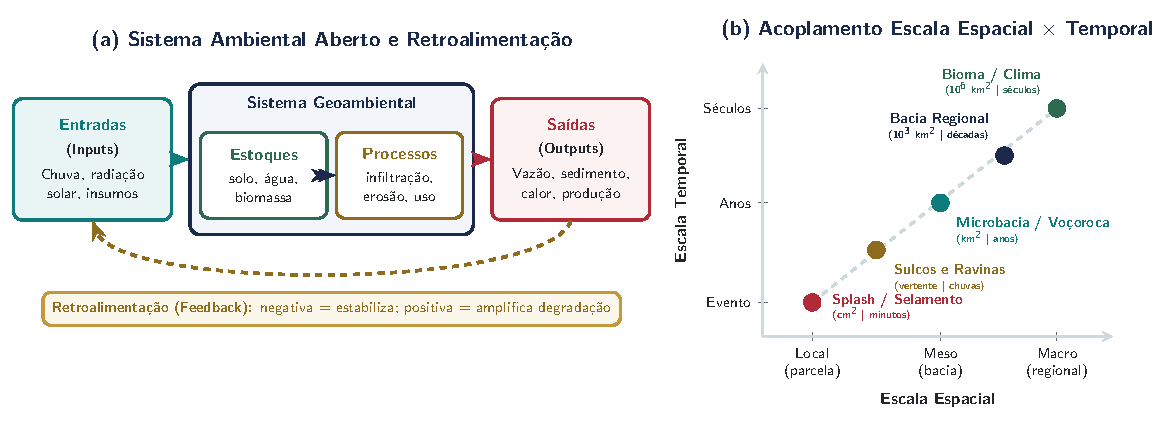
\includegraphics[width=0.95\textwidth]{figures/fig04_sistema_aberto_escalas.pdf}
  \caption{Representação do sistema ambiental aberto com entradas, estoques, processos, saídas e retroalimentação (Painel A) e acoplamento entre escalas espaciais e temporais na dinâmica geoambiental (Painel B). Fonte: elaboração didática da disciplina CHF662 com base em Drew (1989) e Castro; Lemos (2016).}
  \label{fig:sistema_escalas}
\end{figure}

\begin{boxConceito}[Equilíbrio Dinâmico, Limiares (\textit{Thresholds}) e Retroalimentação]
  Em um sistema ambiental aberto, o \textbf{equilíbrio dinâmico (\textit{steady state})} ocorre quando as entradas e saídas se compensam em média ao longo do tempo ($\Delta S \approx 0$), mantendo os estoques estáveis apesar da circulação contínua de água, energia e matéria; trata-se de autorregulação ativa, e não de imobilidade. Essa estabilidade depende da \textbf{retroalimentação negativa (\textit{feedback} negativo)}, mecanismo estabilizador que amortece uma perturbação e devolve o sistema ao estado de referência. Em uma vertente bem vegetada, por exemplo, um aumento moderado de chuva eleva a umidade do solo, estimula o crescimento herbáceo, amplia a interceptação e a infiltração e, por consequência, reduz o escoamento erosivo.

  Em sentido oposto, a \textbf{retroalimentação positiva (\textit{feedback} positivo)} atua como mecanismo amplificador que reforça o desvio inicial, podendo conduzir o sistema à degradação acelerada. Na dinâmica de desertificação ou erosão linear, o sobrepastejo reduz a cobertura vegetal, o que aumenta o selamento e a compactação do solo, derruba a infiltração e eleva o escoamento superficial; essa enxurrada carreia matéria orgânica e sementes, dificulta ainda mais a regeneração vegetal e acelera a abertura de ravinas e voçorocas. Essa transição de regime ocorre quando se ultrapassam \textbf{limiares (\textit{thresholds})}, definidos como pontos críticos de ruptura a partir dos quais o sistema muda de comportamento. Tais limiares podem ser \textbf{extrínsecos}, quando disparados por um evento externo (como uma chuva cuja intensidade ultrapassa a taxa máxima de infiltração do solo, $I > f_c$), ou \textbf{intrínsecos}, quando resultam do enfraquecimento interno gradual do próprio sistema (como o desgaste progressivo da coesão de um talude até o rompimento repentino).
\end{boxConceito}

\section{Escalas Espaciais, Escalas Temporais e o Risco da Falácia de Escala}

Nenhum processo geoambiental ocorre fora de uma escala determinada. Como mostra o Painel B da Figura~\ref{fig:sistema_escalas}, existe um \textbf{acoplamento natural entre escala espacial e escala temporal}: processos microscópicos ou pontuais costumam ocorrer em minutos ou horas, enquanto transformações de bacias regionais e biomas desdobram-se em décadas, séculos ou milênios.

\begin{center}
\renewcommand{\arraystretch}{1.20}
\small
\begin{tabularx}{\textwidth}{@{}p{2.7cm} p{2.5cm} p{2.7cm} >{\raggedright\arraybackslash}X@{}}
  \toprule
  \rowcolor{uefsNavy}
  \textcolor{white}{\bfseries Escala Espacial} & \textcolor{white}{\bfseries Ordem de Área} & \textcolor{white}{\bfseries Escala Temporal Típica} & \textcolor{white}{\bfseries Processos e Aplicações Dominantes} \\
  \midrule
  \textbf{Parcela / Microescala} & $\text{cm}^2$ a $10^2\,\text{m}^2$ & Minutos a horas (evento chuvoso) & Impacto da gota (\textit{splash}), selamento superficial, infiltração pontual e erosão laminar inicial. \\
  \rowcolor{bgGray}
  \textbf{Vertente / Encosta} & $10^2\,\text{m}^2$ a $\text{ha}$ & Chuvas intensas a ciclos sazonais & Escoamento concentrado, formação de sulcos e ravinas, deslizamentos de taludes e manejo conservacionista local. \\
  \textbf{Microbacia} & $1$ a $50\,\text{km}^2$ & Meses a anos (ciclos anuais) & Evolução de voçorocas, conectividade vertente--canal, balanço hídrico local, PRAD e diagnósticos municipais. \\
  \rowcolor{bgGray}
  \textbf{Bacia Regional} & $10^2$ a $10^5\,\text{km}^2$ & Anos a décadas (escala histórica) & Assoreamento de grandes reservatórios, conflitos pelo uso da água, planos de bacia e ZEE estadual. \\
  \textbf{Bioma / Macroescala} & $> 10^5\,\text{km}^2$ & Décadas a milênios (tempo geológico/climático) & Dinâmica climática regional, aridização/desertificação, evolução geomorfológica e grandes políticas territoriais. \\
  \bottomrule
\end{tabularx}
\end{center}

Ignorar o acoplamento entre escalas leva à \textbf{falácia de escala}, um dos erros mais graves na Geografia e na Análise Ambiental, que se manifesta em duas direções opostas. Na \textbf{extrapolação ascendente indevida (micro para macro)}, assume-se que uma taxa de erosão medida em parcela experimental de $10\,\text{m}^2$ multiplica-se linearmente por toda uma bacia de $1\,000\,\text{ha}$; na realidade, grande parte do solo erodido nas encostas fica retida em sopés côncavos, depressões, barreiras vegetais e planícies aluviais antes de atingir o rio principal, fazendo com que a Razão de Entrega de Sedimentos (SDR) seja inferior à unidade. Na \textbf{inferência descendente indevida (macro para micro)}, utiliza-se um mapa de escala pequena ($1:250\,000$ ou $1:1\,000\,000$), elaborado para planejamento estadual, para localizar uma ravina de $4\,\text{m}$ de largura ou projetar uma paliçada de bioengenharia. Em escala cartográfica $1:D$, o menor detalhe graficamente distinguível no papel ($\approx 0{,}2\,\text{mm} = 0{,}0002\,\text{m}$) corresponde no terreno a $d_{\min} = 0{,}0002 \times D$ metros; logo, em uma carta $1:250\,000$, qualquer feição menor que $50\,\text{m}$ desaparece da representação gráfica.

\begin{boxFormula}[Balanço de Massa em Sistema Aberto, Razão de Entrega de Sedimentos (SDR) e Resolução de Escala]
  \textbf{1. Equação geral do balanço em um sistema ambiental aberto:}
  \[
    \Delta S = E - S_{\text{out}}
  \]
  Para o \textbf{balanço hídrico} de uma microbacia (em $\text{mm/ano}$):
  \[
    \Delta S = P - \left(ET + Q_s + Q_b\right)
  \]
  onde $P$ é a precipitação (entrada), $ET$ é a evapotranspiração real, $Q_s$ é o escoamento superficial direto e $Q_b$ é o escoamento de base/drenagem profunda (saídas). Se $\Delta S = 0$, há equilíbrio dinâmico; se $\Delta S < 0$, ocorre depleção do estoque hídrico do solo/aquífero; se $\Delta S > 0$, ocorre recarga.

  \vspace{4pt}
  \textbf{2. Razão de Entrega de Sedimentos (\textit{Sediment Delivery Ratio}, SDR) e quantificação da falácia de escala:}
  \[
    \text{SDR} = \frac{Y}{E_b} \qquad \Longleftrightarrow \qquad Y = E_b \times \text{SDR}, \qquad \text{com } 0 < \text{SDR} \le 1
  \]
  onde $E_b$ é a erosão bruta nas vertentes ($\text{t/(ha}\cdot\text{ano)}$) e $Y$ é a produção específica de sedimentos medida no exutório da bacia ($\text{t/(ha}\cdot\text{ano)}$). Para uma bacia de área $A$ ($\text{ha}$), sendo $E_{b,\text{tot}} = E_b \times A$ a erosão bruta total e $Y_{\text{tot}} = Y \times A$ o aporte total no exutório ($\text{t/ano}$), a massa total retida internamente nas encostas e planícies (colúvios e alúvios) é $R_{\text{sed}} = (E_b - Y) \times A$. Quando um analista extrapola dados de parcela para a bacia assumindo implicitamente $\text{SDR} = 1$, comete erro relativo de superestimativa igual a:
  \[
    \text{Erro (\%)} = \frac{E_{b,\text{tot}} - Y_{\text{tot}}}{Y_{\text{tot}}} \times 100\% = \left(\frac{1}{\text{SDR}} - 1\right) \times 100\%.
  \]

  \vspace{4pt}
  \textbf{3. Menor feição representável em carta de escala $1:D$ (erro gráfico de $0{,}2\,\text{mm}$):}
  \[
    d_{\min}\,(\text{m}) = 0{,}0002 \times D.
  \]
\end{boxFormula}

\section{Dinâmica Geoambiental, Planejamento Ambiental, Planejamento Territorial e Ordenamento Territorial}

Compreender a \textbf{dinâmica geoambiental}, isto é, o comportamento integrado das paisagens frente às pressões climáticas e socioeconômicas, é a base técnica indispensável para orientar decisões públicas sobre o uso do espaço. Contudo, na literatura técnica e em concursos, três expressões correlatas são frequentemente confundidas: \textbf{planejamento ambiental}, \textbf{planejamento territorial} e \textbf{ordenamento territorial} (Arruda, 2013; IBGE, 2018).

\begin{center}
\renewcommand{\arraystretch}{1.22}
\small
\begin{tabularx}{\textwidth}{@{}p{2.9cm} >{\raggedright\arraybackslash}X >{\raggedright\arraybackslash}X p{3.1cm}@{}}
  \toprule
  \rowcolor{uefsNavy}
  \textcolor{white}{\bfseries Conceito} & \textcolor{white}{\bfseries Objeto e foco central} & \textcolor{white}{\bfseries Natureza e função} & \textcolor{white}{\bfseries Instrumentos típicos} \\
  \midrule
  \textbf{Planejamento Ambiental} & Qualidade dos ecossistemas, recursos naturais, fragilidades, riscos e serviços ecossistêmicos. & Processo contínuo de diagnóstico, prognóstico e formulação de diretrizes para conservar, recuperar e compatibilizar atividades humanas à capacidade de suporte ambiental. & AIA, Planos de Bacia Hidrográfica, Planos de Manejo de UCs, PRAD, planos municipais de saneamento e conservação. \\
  \rowcolor{bgGray}
  \textbf{Planejamento Territorial} & Organização socioespacial abrangente (economia, infraestrutura, mobilidade, habitação, redes urbanas e rurais, incluindo a dimensão ambiental). & Processo estratégico multissetorial de definição de cenários, prioridades de investimento e articulação de políticas públicas sobre o território. & Planos Diretores Municipais, Planos de Desenvolvimento Regional, Planos Plurianuais territorializados. \\
  \textbf{Ordenamento Territorial} & Regulação espacial efetiva da distribuição das atividades, usos do solo e ocupação humana no território. & Expressão \textbf{normativa, cartográfica e vinculante} do Estado para compatibilizar usos produtivos, infraestrutura e proteção ambiental, reduzindo conflitos socioespaciais. & \textbf{Zoneamento Ecológico-Econômico (ZEE)}, macrozoneamento do Plano Diretor, zoneamento costeiro e agrícola. \\
  \bottomrule
\end{tabularx}
\end{center}

Em síntese operacional, o \textbf{planejamento ambiental} define os limites, potenciais e fragilidades dos sistemas naturais; o \textbf{planejamento territorial} integra esses condicionantes às demandas econômicas, sociais e de infraestrutura; e o \textbf{ordenamento territorial} traduz essas diretrizes em normas espaciais e zoneamentos concretos de regulação do uso da terra.

\section{Zoneamento Ecológico-Econômico (ZEE) como Instrumento de Ordenamento}

Previsto originalmente na Política Nacional do Meio Ambiente (Lei nº 6.938/1981) e regulamentado pelo \textbf{Decreto Federal nº 4.297/2002}, o \textbf{Zoneamento Ecológico-Econômico (ZEE)} é o principal instrumento técnico-político de organização do território no Brasil. Longe de constituir um conjunto estático de restrições ou um documento meramente cartográfico, o ZEE opera como um processo participativo e multidisciplinar que cruza a \textbf{potencialidade socioeconômica} com a \textbf{vulnerabilidade e fragilidade natural} dos sistemas geoambientais (IBGE, 2018; Arruda, 2013).

A partir desse cruzamento, o território é dividido em \textbf{zonas homogêneas} com regras específicas de uso, manejo e investimento público. As \textbf{Zonas de Consolidação Produtiva} reúnem áreas de alta aptidão e baixa fragilidade natural, nas quais o uso agropecuário, industrial ou urbano deve ser otimizado com boas práticas de conservação de solo e água. Já as \textbf{Zonas de Uso Restrito ou Manejo Sustentável} correspondem a áreas de fragilidade média a alta que admitem atividades produtivas de baixo impacto, como extrativismo sustentável, sistemas agroflorestais, ecoturismo e manejo da Caatinga. Em áreas já submetidas a processos de degradação (erosão acelerada, desertificação e matas ciliares suprimidas), instituem-se \textbf{Zonas de Recuperação Ambiental}, prioritárias para PRAD, bioengenharia e recomposição florestal. Por sua vez, as \textbf{Zonas de Proteção e Conservação} abrangem setores de altíssima fragilidade, relevância hídrica ou biodiversidade endêmica (APPs, nascentes, Unidades de Conservação e corredores ecológicos), voltados prioritariamente à preservação.

O ZEE dialoga diretamente com a AIA (Capítulo 5), pois, quando um estado ou município dispõe de um ZEE atualizado em escala compatível, a etapa de triagem e a seleção de alternativas locacionais tornam-se muito mais céleres, transparentes e seguras juridicamente.

% ============================================================================
% ETAPA 4 — ESTUDOS DE CASO E EXEMPLOS RESOLVIDOS (5 EXEMPLOS, 7 PASSOS CADA)
% ============================================================================
\etapa{4}{Estudos de Caso e Exemplos Resolvidos Passo a Passo}

\begin{boxExemplo}{6.1}{Balanço Hídrico em Sistema Ambiental Aberto no Semiárido (Nível Básico)}
  \passoEnunciado{Uma microbacia experimental inserida no domínio da Caatinga foi monitorada durante um ano hidrológico completo. Deseja-se avaliar se o sistema hídrico local operou em equilíbrio dinâmico, recarga ou depleção de estoque.}
  \passoDados{Entrada anual de precipitação $P = 680\,\text{mm/ano}$. Saídas anuais medidas: evapotranspiração real $ET = 545\,\text{mm/ano}$; escoamento superficial direto $Q_s = 115\,\text{mm/ano}$; escoamento de base / drenagem profunda $Q_b = 35\,\text{mm/ano}$.}
  \passoPedido{Calcular o total de saídas ($S_{\text{out}}$), a variação do estoque hídrico interno ($\Delta S$) e interpretar o estado funcional do sistema nesse ano hidrológico.}
  \passoMetodo{Aplicação da equação de conservação de massa em sistema ambiental aberto: $\Delta S = P - (ET + Q_s + Q_b)$.}
  \passoContas{%
    \begin{enumerate}[leftmargin=1.5em, itemsep=2pt]
      \item \textbf{Soma das saídas do sistema ($S_{\text{out}}$):}
      \[
        S_{\text{out}} = ET + Q_s + Q_b = 545 + 115 + 35 = 695\,\text{mm/ano}.
      \]
      \item \textbf{Variação do estoque hídrico ($\Delta S$):}
      \[
        \Delta S = P - S_{\text{out}} = 680 - 695 = -15\,\text{mm/ano}.
      \]
      \item \textbf{Interpretação física:} o sinal negativo ($\Delta S = -15\,\text{mm/ano}$) indica que as saídas superaram as entradas em $15\,\text{mm}$; logo, o sistema consumiu parte da água armazenada previamente no solo e nos reservatórios subterrâneos rasos (depleção líquida de estoque).
    \end{enumerate}
  }
  \passoResposta{Total de saídas $S_{\text{out}} = 695\,\text{mm/ano}$ e variação do estoque $\Delta S = -15\,\text{mm/ano}$, caracterizando depleção moderada do estoque hídrico interno nesse ano.}
  \passoVerificacao{O valor é fisicamente coerente para o Semiárido baiano: a evapotranspiração consome a maior parcela da chuva ($545/680 \approx 80{,}15\%$), e déficits interanuais moderados de estoque são esperados em anos de precipitação ligeiramente abaixo da média, sendo compensados nos anos mais chuvosos se a cobertura vegetal preservar a infiltração.}
\end{boxExemplo}

\begin{boxExemplo}{6.2}{Quantificando a Falácia de Escala pela Razão de Entrega de Sedimentos: SDR (Nível Básico–Intermediário)}
  \passoEnunciado{Em uma parcela experimental de $20\,\text{m}^2$ de solo exposto em uma microbacia do Piemonte da Diamantina, mediu-se uma taxa de erosão bruta de $E_b = 24{,}0\,\text{t/(ha}\cdot\text{ano)}$. Para estimar o assoreamento de um açude no exutório da bacia (área total $A = 1\,500\,\text{ha}$), um técnico multiplicou diretamente a taxa da parcela pela área da bacia. Entretanto, o monitoramento hidrossedimentológico no exutório registrou uma chegada efetiva de $Y_{\text{tot}} = 9\,720\,\text{t/ano}$.}
  \passoDados{$E_b = 24{,}0\,\text{t/(ha}\cdot\text{ano)}$; área da bacia $A = 1\,500\,\text{ha}$; produção total medida no exutório $Y_{\text{tot}} = 9\,720\,\text{t/ano}$.}
  \passoPedido{Calcular: (a) a erosão bruta total estimada pela extrapolação linear do técnico; (b) a produção específica real $Y$; (c) a Razão de Entrega de Sedimentos (SDR); (d) a massa anual de sedimentos retida nas vertentes e planícies; e (e) o erro percentual causado pela falácia de escala.}
  \passoMetodo{Aplicação das relações de escala hidrossedimentológica: $E_{b,\text{tot}} = E_b \cdot A$, $Y = Y_{\text{tot}}/A$, $\text{SDR} = Y / E_b$, $R_{\text{sed}} = E_{b,\text{tot}} - Y_{\text{tot}}$ e $\text{Erro (\%)} = (E_{b,\text{tot}} - Y_{\text{tot}})/Y_{\text{tot}} \times 100\%$.}
  \passoContas{%
    \begin{enumerate}[leftmargin=1.5em, itemsep=2pt]
      \item \textbf{Extrapolação linear do técnico (erosão bruta total):}
      \[
        E_{b,\text{tot}} = 24{,}0\,\text{t/(ha}\cdot\text{ano)} \times 1\,500\,\text{ha} = 36\,000\,\text{t/ano}.
      \]
      \item \textbf{Produção específica real de sedimentos no exutório ($Y$):}
      \[
        Y = \frac{9\,720\,\text{t/ano}}{1\,500\,\text{ha}} = 6{,}48\,\text{t/(ha}\cdot\text{ano)}.
      \]
      \item \textbf{Razão de Entrega de Sedimentos (SDR):}
      \[
        \text{SDR} = \frac{Y}{E_b} = \frac{6{,}48}{24{,}0} = 0{,}27 \quad (\text{ou } 27\%).
      \]
      \item \textbf{Massa de sedimentos retida internamente na bacia:}
      \[
        R_{\text{sed}} = 36\,000 - 9\,720 = 26\,280\,\text{t/ano} \quad (73\% \text{ do solo mobilizado}).
      \]
      \item \textbf{Erro percentual de superestimativa (falácia de escala):}
      \[
        \text{Erro (\%)} = \frac{36\,000 - 9\,720}{9\,720} \times 100\% = \frac{26\,280}{9\,720} \times 100\% \approx 270{,}37\%.
      \]
    \end{enumerate}
  }
  \passoResposta{$E_{b,\text{tot}} = 36\,000\,\text{t/ano}$; $Y = 6{,}48\,\text{t/(ha}\cdot\text{ano)}$; $\text{SDR} = 0{,}27$; sedimentos retidos $= 26\,280\,\text{t/ano}$; erro de superestimativa $= 270{,}37\%$.}
  \passoVerificacao{Confere-se a fórmula alternativa do erro: $(1/\text{SDR} - 1)\times 100\% = (1/0{,}27 - 1)\times 100\% = (3{,}7037 - 1)\times 100\% = 270{,}37\%$. Ambientalmente, esse resultado demonstra a essência da \textbf{falácia de escala}: taxas medidas em parcela de $20\,\text{m}^2$ não consideram a rede de deposição em sopés, depressões e matas ciliares que retém $73\%$ dos sedimentos ao longo de uma bacia de $1\,500\,\text{ha}$.}
\end{boxExemplo}

\begin{boxExemplo}{6.3}{Limiar de Infiltração e Retroalimentação Positiva versus Negativa (Nível Intermediário)}
  \passoEnunciado{Duas vertentes vizinhas com mesma litologia e declividade no Semiárido baiano recebem a mesma chuva convectiva intensa de $I = 65{,}0\,\text{mm/h}$ durante $1$ hora. A \textbf{Vertente 1} possui cobertura de Caatinga conservada com serrapilheira e capacidade de infiltração estável $f_{c1} = 78{,}0\,\text{mm/h}$. A \textbf{Vertente 2} foi submetida a sobrepastejo contínuo, apresentando solo compactado com capacidade de infiltração reduzida para $f_{c2} = 22{,}0\,\text{mm/h}$.}
  \passoDados{Intensidade da chuva $I = 65{,}0\,\text{mm/h}$; limiar de infiltração da Vertente 1: $f_{c1} = 78{,}0\,\text{mm/h}$; limiar de infiltração da Vertente 2: $f_{c2} = 22{,}0\,\text{mm/h}$.}
  \passoPedido{Calcular o excesso de precipitação transformado em escoamento superficial ($R = \max(0, I - f_c)$) e o percentual da chuva que escoa superficialmente em cada vertente, identificando em qual delas o limiar extrínseco foi rompido e qual tipo de retroalimentação predomina.}
  \passoMetodo{Comparação direta entre a entrada externa ($I$) e o limiar interno de infiltração ($f_c$), seguida da análise sistêmica dos circuitos de retroalimentação.}
  \passoContas{%
    \begin{enumerate}[leftmargin=1.5em, itemsep=2pt]
      \item \textbf{Vertente 1 (Caatinga conservada):}
      Como $I = 65{,}0\,\text{mm/h} < f_{c1} = 78{,}0\,\text{mm/h}$, o limiar de infiltração \textbf{não é ultrapassado}:
      \[
        R_1 = \max(0,\; 65{,}0 - 78{,}0) = 0{,}0\,\text{mm/h} \quad (0\% \text{ de escoamento hortoniano}).
      \]
      Toda a lâmina de $65{,}0\,\text{mm}$ infiltra-se, recarregando a umidade do solo, sustentando a vegetação e mantendo a estrutura porosa (\textbf{retroalimentação negativa}, estabilizadora).
      \item \textbf{Vertente 2 (Pastagem compactada):}
      Como $I = 65{,}0\,\text{mm/h} > f_{c2} = 22{,}0\,\text{mm/h}$, o limiar de infiltração é \textbf{rompido}:
      \[
        R_2 = 65{,}0 - 22{,}0 = 43{,}0\,\text{mm/h}.
      \]
      \item \textbf{Percentual da chuva convertido em escoamento superficial na Vertente 2:}
      \[
        \frac{R_2}{I} \times 100\% = \frac{43{,}0}{65{,}0} \times 100\% \approx 66{,}15\%.
      \]
      Mais de dois terços da chuva escoam velozmente pela superfície, removendo solo fértil, sementes e nutrientes, o que dificulta a regeneração vegetal e reduz ainda mais $f_c$ nas chuvas seguintes (\textbf{retroalimentação positiva}, amplificadora da degradação).
    \end{enumerate}
  }
  \passoResposta{Vertente 1: $R_1 = 0{,}0\,\text{mm/h}$ ($0\%$, abaixo do limiar, retroalimentação negativa). Vertente 2: $R_2 = 43{,}0\,\text{mm/h}$ ($66{,}15\%$ da chuva vira enxurrada, limiar rompido, retroalimentação positiva degradativa).}
  \passoVerificacao{O contraste entre $0\,\text{mm/h}$ e $43{,}0\,\text{mm/h}$ sob exatamente a mesma chuva demonstra que a degradação no Semiárido não decorre apenas da ``força da natureza'', mas da interação entre o evento climático (meio físico) e o manejo do solo/vegetação (meios biótico e antrópico).}
\end{boxExemplo}

\begin{boxExemplo}{6.4}{Escolha de Escala Cartográfica e Erro Gráfico Mínimo em Diagnósticos (Nível Intermediário–Avançado)}
  \passoEnunciado{Uma equipe de Geografia precisa mapear ravinas com largura média de $4{,}0\,\text{m}$ e faixas de mata ciliar de $15{,}0\,\text{m}$ em uma microbacia de $850\,\text{ha}$ ($8{,}5\,\text{km}^2$) próxima a Feira de Santana. A prefeitura dispõe de três bases cartográficas: uma carta regional do ZEE ($1:250\,000$), uma carta topográfica sistemática ($1:50\,000$) e um ortomosaico detalhado ($1:10\,000$).}
  \passoDados{Erro gráfico mínimo no papel $= 0{,}2\,\text{mm} = 0{,}0002\,\text{m}$; escalas disponíveis: $D_1 = 250\,000$, $D_2 = 50\,000$ e $D_3 = 10\,000$; alvos de mapeamento: ravinas ($4{,}0\,\text{m}$) e mata ciliar ($15{,}0\,\text{m}$).}
  \passoPedido{Calcular a menor feição representável no terreno ($d_{\min}$) em cada escala e determinar qual base é tecnicamente adequada para mapear os dois alvos sem incorrer em falácia de escala.}
  \passoMetodo{Aplicação da relação de resolução gráfica cartográfica $d_{\min} = 0{,}0002 \times D$ e comparação direta com a largura real das feições-alvo.}
  \passoContas{%
    \begin{enumerate}[leftmargin=1.5em, itemsep=2pt]
      \item \textbf{Carta regional ($1:250\,000$):}
      \[
        d_{\min,1} = 0{,}0002 \times 250\,000 = 50{,}0\,\text{m}.
      \]
      Nem a mata ciliar ($15{,}0\,\text{m} < 50{,}0\,\text{m}$) nem as ravinas ($4{,}0\,\text{m} < 50{,}0\,\text{m}$) podem ser representadas com fidelidade geométrica.
      \item \textbf{Carta topográfica municipal ($1:50\,000$):}
      \[
        d_{\min,2} = 0{,}0002 \times 50\,000 = 10{,}0\,\text{m}.
      \]
      A mata ciliar ($15{,}0\,\text{m} > 10{,}0\,\text{m}$) já é representável, porém as ravinas ($4{,}0\,\text{m} < 10{,}0\,\text{m}$) permanecem abaixo do limite gráfico.
      \item \textbf{Base detalhada ($1:10\,000$):}
      \[
        d_{\min,3} = 0{,}0002 \times 10\,000 = 2{,}0\,\text{m}.
      \]
      Tanto a mata ciliar ($15{,}0\,\text{m} > 2{,}0\,\text{m}$) quanto as ravinas ($4{,}0\,\text{m} > 2{,}0\,\text{m}$) são representáveis em escala real.
    \end{enumerate}
  }
  \passoResposta{As menores feições representáveis são $50{,}0\,\text{m}$ ($1:250\,000$), $10{,}0\,\text{m}$ ($1:50\,000$) e $2{,}0\,\text{m}$ ($1:10\,000$). Somente a escala $1:10\,000$ (ou maior detalhe, como $1:5\,000$ obtida por drone/VANT) permite mapear simultaneamente as ravinas de $4{,}0\,\text{m}$ e a mata ciliar de $15{,}0\,\text{m}$.}
  \passoVerificacao{Concluir que ``não existem ravinas na microbacia'' após inspecionar uma carta $1:250\,000$ seria um exemplo clássico de falácia de escala descendente: a ausência no mapa reflete a limitação da escala escolhida, não a inexistência do processo erosivo em campo.}
\end{boxExemplo}

\begin{boxExemplo}{6.5}{Zoneamento Ecológico-Econômico (ZEE) e Articulação com o Ordenamento Territorial (Nível Avançado)}
  \passoEnunciado{Após integrar levantamentos de solos, declividade, remanescentes de Caatinga, recursos hídricos e uso agropecuário, um município baiano de $1\,200\,\text{km}^2$ elaborou sua proposta de Zoneamento Ecológico-Econômico (ZEE), distribuindo o território em quatro zonas.}
  \passoDados{Área total do município $= 1\,200\,\text{km}^2$:
  \begin{itemize}[leftmargin=1.5em, itemsep=1.5pt]
    \item $Z_1$, Zona de Consolidação Produtiva: $420\,\text{km}^2$;
    \item $Z_2$, Zona de Expansão com Manejo Sustentável: $330\,\text{km}^2$;
    \item $Z_3$, Zona de Recuperação Ambiental (áreas degradadas/erosão): $210\,\text{km}^2$;
    \item $Z_4$, Zona de Proteção e Conservação (nascentes, serras e UCs): $240\,\text{km}^2$.
  \end{itemize}}
  \passoPedido{Verificar o fechamento territorial das áreas, calcular o percentual de cada zona, determinar o percentual conjunto destinado à conservação e recuperação ($Z_3 + Z_4$) e distinguir o papel do planejamento ambiental, do planejamento territorial e do ordenamento territorial nesse caso.}
  \passoMetodo{Cálculo de participação percentual ($A_k / A_{\text{total}} \times 100\%$) e classificação funcional conforme Arruda (2013) e IBGE (2018).}
  \passoContas{%
    \begin{enumerate}[leftmargin=1.5em, itemsep=2pt]
      \item \textbf{Verificação da soma das áreas:} $420 + 330 + 210 + 240 = 1\,200\,\text{km}^2$ ($100{,}0\%$, fechamento exato).
      \item \textbf{Percentual de cada zona:}
      \begin{align*}
        \%Z_1 &= \frac{420}{1\,200} \times 100\% = 35{,}0\%, & \%Z_2 &= \frac{330}{1\,200} \times 100\% = 27{,}5\%, \\
        \%Z_3 &= \frac{210}{1\,200} \times 100\% = 17{,}5\%, & \%Z_4 &= \frac{240}{1\,200} \times 100\% = 20{,}0\%.
      \end{align*}
      \item \textbf{Soma das zonas de proteção e recuperação ($Z_3 + Z_4$):}
      \[
        A_{3+4} = 210 + 240 = 450\,\text{km}^2 \implies \frac{450}{1\,200} \times 100\% = 37{,}5\% \quad (\text{ou } 17{,}5\% + 20{,}0\% = 37{,}5\%).
      \]
      \item \textbf{Articulação conceitual:} o \textbf{planejamento ambiental} forneceu o diagnóstico integrado de solos, nascentes, fragilidades e áreas degradadas ($Z_3$ e $Z_4$); o \textbf{planejamento territorial} compatibilizou essas informações com as metas de produção agropecuária, estradas e abastecimento urbano ($Z_1$ e $Z_2$); o \textbf{ordenamento territorial} normatizou o mapa final do ZEE em lei/decreto, vinculando licenciamento ambiental, crédito rural e investimentos públicos às regras de cada zona.
    \end{enumerate}
  }
  \passoResposta{$Z_1 = 35{,}0\%$, $Z_2 = 27{,}5\%$, $Z_3 = 17{,}5\%$ e $Z_4 = 20{,}0\%$; conservação e recuperação somam $450\,\text{km}^2$ ($37{,}5\%$ do município). O ZEE materializa o ordenamento territorial apoiado pelos planejamentos ambiental e territorial.}
  \passoVerificacao{A soma dos percentuais fecha em $35{,}0 + 27{,}5 + 17{,}5 + 20{,}0 = 100{,}0\%$. Territorialmente, reservar $37{,}5\%$ para proteção e recuperação enquanto se direcionam $62{,}5\%$ para produção consolidada e manejo sustentável mostra que o ZEE não paralisa o desenvolvimento econômico, mas o redireciona para áreas com capacidade de suporte adequada.}
\end{boxExemplo}

% ============================================================================
% ETAPA 5 — ERROS MAIS COMUNS (4 BOXES)
% ============================================================================
\etapa{5}{Erros Mais Comuns em Análise Integrada, Escalas e Ordenamento}

\begin{boxErro}[Erro 1: Confundir retroalimentação positiva com algo ``bom'' ou desejável]
  \textbf{Equívoco frequente:} interpretar ``retroalimentação positiva'' como um processo ambientalmente benéfico e ``retroalimentação negativa'' como algo prejudicial.
  \par\textbf{Por que está incorreto:} na Teoria dos Sistemas, os adjetivos \emph{positivo} e \emph{negativo} têm sentido matemático/cibernético, não moral. \textbf{Negativa} significa que o retorno \emph{opõe-se} ao desvio inicial e estabiliza o sistema; \textbf{positiva} significa que o retorno \emph{soma-se} ao desvio inicial e o amplifica, constituindo o motor típico de voçorocamentos, desertificação e colapsos ecológicos.
  \par\textbf{Como evitar:} associe sempre \textbf{negativa = freio estabilizador} e \textbf{positiva = acelerador/bola de neve}.
\end{boxErro}

\begin{boxErro}[Erro 2: Praticar a falácia de escala extrapolando dados de parcela diretamente para a bacia]
  \textbf{Equívoco frequente:} multiplicar a perda de solo medida em parcela de $10\,\text{m}^2$ pela área inteira de uma bacia de $5\,000\,\text{ha}$ e afirmar que toda aquela massa chegará ao rio principal.
  \par\textbf{Por que está incorreto:} ignora os estoques intermediários e a deposição ao longo das encostas e planícies (Razão de Entrega de Sedimentos $\text{SDR} < 1$). Do mesmo modo, utilizar cartas regionais ($1:250\,000$) para diagnosticar feições de poucos metros omite processos críticos locais.
  \par\textbf{Como evitar:} explicite sempre a escala espacial e temporal da medição e verifique se o modelo ou a carta escolhida possui resolução compatível com o fenômeno analisado.
\end{boxErro}

\begin{boxErro}[Erro 3: Reduzir a Análise Ambiental Integrada à soma de relatórios setoriais desconexos]
  \textbf{Equívoco frequente:} entregar um trabalho com uma seção de geologia, uma de vegetação e uma de população que nunca se referenciam entre si.
  \par\textbf{Por que está incorreto:} sem explicitar como a declividade e o solo respondem à retirada da vegetação e como isso repercute no uso da terra e na oferta hídrica, não há análise integrada, apenas um inventário descritivo fragmentado.
  \par\textbf{Como evitar:} ao redigir qualquer diagnóstico, use verbos de processo e encadeamento (infiltra, concentra, carreia, protege, amplifica, restringe) conectando explicitamente os meios físico, biótico e antrópico.
\end{boxErro}

\begin{boxErro}[Erro 4: Tratar planejamento ambiental, planejamento territorial e ordenamento territorial como sinônimos]
  \textbf{Equívoco frequente:} usar os três termos de maneira intercambiável em provas ou confundir ZEE com simples criação de Unidades de Conservação.
  \par\textbf{Por que está incorreto:} embora articulados, possuem recortes distintos: o planejamento ambiental foca processos e limites ecológicos; o planejamento territorial integra todas as dimensões socioespaciais e de infraestrutura; o ordenamento territorial corresponde à regulação espacial normativa do uso da terra (tendo no ZEE um instrumento que abrange tanto zonas produtivas quanto zonas de recuperação e conservação).
  \par\textbf{Como evitar:} memorize a tríade funcional: \emph{limites ambientais} (planejamento ambiental) $\to$ \emph{estratégia multissetorial} (planejamento territorial) $\to$ \emph{regulação espacial normativa} (ordenamento territorial / ZEE).
\end{boxErro}

% ============================================================================
% ETAPA 6 — EXERCÍCIOS DE FIXAÇÃO (15 EXERCÍCIOS: 5 BÁSICOS, 5 INTERM., 5 OBJ.)
% ============================================================================
\etapa{6}{Exercícios de Fixação}

\subsection*{Nível 1: Básico (Sistemas Abertos, Escalas e Ordenamento)}

\begin{enumerate}[leftmargin=1.8em, itemsep=4pt]
  \item Explique por que uma bacia hidrográfica é classificada como um \textbf{sistema ambiental aberto}, exemplificando duas entradas, dois estoques internos, dois processos e duas saídas.
  \espacoResolucao[2.0cm]

  \item Diferencie \textbf{retroalimentação negativa} e \textbf{retroalimentação positiva} em sistemas ambientais, apresentando um exemplo concreto de cada mecanismo na dinâmica erosiva de uma encosta.
  \espacoResolucao[2.0cm]

  \item Um açude no Semiárido baiano recebeu em um ano $E = 12\,500\,\text{t/ano}$ de sedimentos transportados pelos riachos afluentes e exportou pelo vertedouro $S_{\text{out}} = 3\,200\,\text{t/ano}$. Calcule a variação do estoque de sedimentos retidos no reservatório ($\Delta S$) e a eficiência percentual de retenção de sedimentos do açude.
  \espacoResolucao[2.1cm]

  \item O que é \textbf{falácia de escala} na Análise Ambiental? Dê um exemplo de erro cometido ao passar da microescala para a macroescala e outro ao passar da macroescala para a microescala.
  \espacoResolucao[2.1cm]

  \item Estabeleça a diferença conceitual entre \textbf{planejamento ambiental}, \textbf{planejamento territorial} e \textbf{ordenamento territorial}, situando o papel do Zoneamento Ecológico-Econômico (ZEE).
  \espacoResolucao[2.2cm]
\end{enumerate}

\subsection*{Nível 2: Intermediário (Cálculos Sistêmicos, Escalas e ZEE)}

\begin{enumerate}[leftmargin=1.8em, itemsep=4pt, resume]
  \item Em uma microbacia de $800\,\text{ha}$, a erosão bruta média das vertentes estimada por parcelas é $E_b = 18{,}0\,\text{t/(ha}\cdot\text{ano)}$. Sabe-se que a Razão de Entrega de Sedimentos da microbacia é $\text{SDR} = 0{,}32$. Calcule: (a) a erosão bruta total ($E_{b,\text{tot}}$); (b) a produção específica ($Y$) e total ($Y_{\text{tot}}$) de sedimentos no exutório; (c) a massa anual retida nas vertentes e planícies; e (d) o erro percentual de superestimativa que ocorreria caso um analista assumisse $\text{SDR} = 1$.
  \espacoResolucao[2.8cm]

  \item Uma mesma microbacia recebeu precipitação anual de $P = 750\,\text{mm/ano}$ em dois cenários de cobertura do solo:
  \begin{itemize}[leftmargin=1.4em, itemsep=1pt]
    \item \textbf{Cenário 1 (Vegetação nativa conservada):} $ET = 590\,\text{mm}$, $Q_s = 90\,\text{mm}$, $Q_b = 70\,\text{mm}$.
    \item \textbf{Cenário 2 (Após desmatamento e compactação):} $ET = 430\,\text{mm}$, $Q_s = 340\,\text{mm}$, $Q_b = 25\,\text{mm}$.
  \end{itemize}
  Calcule $\Delta S$ em ambos os cenários, determine que percentual da chuva virou escoamento superficial ($Q_s/P$) no Cenário 2 e interprete as consequências para a vazão na estiagem ($Q_b$) e para a erosão.
  \espacoResolucao[2.8cm]

  \item Utilizando o erro gráfico mínimo de $0{,}2\,\text{mm}$ no papel ($d_{\min} = 0{,}0002 \times D$), calcule a menor feição representável no terreno para as escalas $1:100\,000$, $1:25\,000$ e $1:5\,000$. Em seguida, informe quais dessas escalas conseguem representar: (a) uma faixa de mata ciliar de $15{,}0\,\text{m}$ de largura; (b) uma ravina incipiente de $1{,}5\,\text{m}$ de largura.
  \espacoResolucao[2.5cm]

  \item Explique a diferença entre \textbf{limiar extrínseco} e \textbf{limiar intrínseco} na dinâmica geoambiental, ilustrando cada tipo com um processo real de instabilidade de encostas ou erosão no Brasil.
  \espacoResolucao[2.2cm]

  \item O ZEE de uma sub-bacia hidrográfica de $2\,500\,\text{km}^2$ definiu a seguinte repartição percentual: $40\%$ de Zona de Consolidação Produtiva, $26\%$ de Zona de Manejo Sustentável, $16\%$ de Zona de Recuperação Ambiental e $18\%$ de Zona de Proteção e Conservação. Calcule a área em $\text{km}^2$ de cada zona e verifique se o plano atende a uma diretriz estadual que exige no mínimo $30\%$ do território sob conservação ou recuperação.
  \espacoResolucao[2.4cm]
\end{enumerate}

\subsection*{Nível 3: Questões Objetivas de Fixação (A–E)}

\begin{enumerate}[leftmargin=1.8em, itemsep=5pt, resume]
  \item \textbf{[Autoral, CHF662]} Em uma vertente degradada do Semiárido, a remoção da Caatinga expõe o solo ao impacto das gotas de chuva, gerando crosta superficial, redução da infiltração, aumento da enxurrada e carreamento de matéria orgânica, o que impede a germinação de novas plantas e intensifica ainda mais a erosão. Na teoria dos sistemas ambientais, esse encadeamento caracteriza:
  \begin{alternativas}
    \item Sistema fechado em equilíbrio termodinâmico estático.
    \item Retroalimentação negativa de autorregulação ecológica.
    \item Retroalimentação positiva amplificadora da degradação.
    \item Neutralidade escalar sem rompimento de limiar.
    \item Ciclo biogeoquímico conservativo com ganho de estoque edáfico.
  \end{alternativas}
  \espacoResolucao[1.2cm]

  \item \textbf{[Autoral, CHF662]} Sobre o acoplamento entre escalas espaciais e temporais na Análise Ambiental Integrada, assinale a alternativa correta:
  \begin{alternativas}
    \item Processos como o impacto da gota de chuva (\textit{splash}) e o selamento superficial atuam na macroescala continental ao longo de milênios.
    \item A dinâmica de uma microbacia ou a evolução de voçorocas manifestam-se tipicamente na escala local a mesoescala, ao longo de meses e anos.
    \item A escala temporal é independente da escala espacial, podendo qualquer processo ser monitorado em um único dia de campo.
    \item Cartas na escala $1:1\,000\,000$ são ideais para medir a largura de sulcos erosivos em pequenas propriedades rurais.
    \item O estudo de biomas prescinde de séries históricas pluridecadais por depender apenas de eventos horários isolados.
  \end{alternativas}
  \espacoResolucao[1.2cm]

  \item \textbf{[Autoral, CHF662]} Qual alternativa distingue corretamente \textbf{ordenamento territorial} de \textbf{planejamento ambiental}?
  \begin{alternativas}
    \item O ordenamento territorial restringe-se ao monitoramento químico da água, enquanto o planejamento ambiental define a malha rodoviária.
    \item O planejamento ambiental diagnostica fragilidades, riscos e capacidades de suporte dos ecossistemas, ao passo que o ordenamento territorial traduz diretrizes socioespaciais e ambientais em regulação normativa e espacial dos usos da terra (como o ZEE).
    \item O ordenamento territorial é facultativo e exclusivamente acadêmico, enquanto o planejamento ambiental não utiliza mapas.
    \item O planejamento ambiental proíbe qualquer atividade produtiva, enquanto o ordenamento territorial dispensa critérios ecológicos.
    \item Ambos são sinônimos perfeitos de licenciamento ambiental de obras pontuais.
  \end{alternativas}
  \espacoResolucao[1.2cm]

  \item \textbf{[Autoral, CHF662]} Em uma bacia de $600\,\text{ha}$, medições em parcela indicaram erosão bruta de $15{,}0\,\text{t/(ha}\cdot\text{ano)}$. Sabendo que a Razão de Entrega de Sedimentos da bacia é $\text{SDR} = 0{,}40$, a produção anual de sedimentos que efetivamente chega ao exutório e a massa retida internamente nas vertentes e planícies são, respectivamente:
  \begin{alternativas}
    \item $9\,000\,\text{t/ano}$ e $0\,\text{t/ano}$.
    \item $5\,400\,\text{t/ano}$ e $3\,600\,\text{t/ano}$.
    \item $3\,600\,\text{t/ano}$ e $5\,400\,\text{t/ano}$.
    \item $2\,400\,\text{t/ano}$ e $6\,600\,\text{t/ano}$.
    \item $6\,000\,\text{t/ano}$ e $3\,000\,\text{t/ano}$.
  \end{alternativas}
  \espacoResolucao[1.2cm]

  \item \textbf{[Autoral, CHF662]} De acordo com o Decreto Federal nº 4.297/2002 e os fundamentos do IBGE (2018), o \textbf{Zoneamento Ecológico-Econômico (ZEE)} caracteriza-se por:
  \begin{alternativas}
    \item Ser um mapa exclusivamente voltado à demarcação de parques nacionais, excluindo áreas agrícolas e urbanas.
    \item Integrar potencialidades socioeconômicas e vulnerabilidades/fragilidades geoambientais para dividir o território em zonas com diretrizes específicas de uso, manejo, recuperação e proteção.
    \item Substituir a obrigatoriedade do Estudo de Impacto Ambiental (EIA) para grandes hidrelétricas e minerações.
    \item Operar apenas na escala de parcela experimental ($1:500$), sendo inviável em estados ou bacias regionais.
    \item Utilizar apenas variáveis climáticas, dispensando informações de solos, relevo e estrutura social.
  \end{alternativas}
  \espacoResolucao[1.2cm]
\end{enumerate}

% ============================================================================
% ETAPA 7 — QUESTÕES DE PROVAS, ENADE E CONCURSOS AMBIENTAIS (3 AUTORAIS)
% ============================================================================
\etapa{7}{Questões no Estilo ENADE e Concursos Ambientais}

\begin{enumerate}[leftmargin=1.8em, itemsep=5pt, resume]
  \item \textbf{[Autoral, Estilo ENADE / Geografia]} A abordagem sistêmica aplicada à Análise Ambiental Integrada (Drew, 1989; Castro; Lemos, 2016) compreende a paisagem como resultado de interações dinâmicas entre fluxos de matéria, energia e decisões humanas. Avalie as asserções a seguir e a relação proposta entre elas:
  \begin{quote}
    \textbf{I.} A extrapolação linear de taxas de perda de solo obtidas em pequenas parcelas experimentais para grandes bacias hidrográficas costuma superestimar significativamente o aporte real de sedimentos no exutório.
    \par\vspace{3pt}
    \textbf{PORQUE}
    \par\vspace{3pt}
    \textbf{II.} Ao mudar da escala de parcela para a escala de bacia, emergem processos intermediários de desconectividade e deposição em sopés, depressões, barreiras vegetais e planícies aluviais, fazendo com que a Razão de Entrega de Sedimentos (SDR) seja inferior a $1$.
  \end{quote}
  A respeito dessas asserções, assinale a opção correta:
  \begin{alternativas}
    \item As asserções I e II são proposições verdadeiras, e a II é uma justificativa correta da I.
    \item As asserções I e II são proposições verdadeiras, mas a II não é uma justificativa correta da I.
    \item A asserção I é uma proposição verdadeira, e a II é uma proposição falsa.
    \item A asserção I é uma proposição falsa, e a II é uma proposição verdadeira.
    \item As asserções I e II são proposições falsas.
  \end{alternativas}
  \espacoResolucao[1.2cm]

  \item \textbf{[Autoral, Estilo Concurso Geógrafo / Planejamento Territorial]} Considere o balanço de um sistema ambiental aberto sujeito a intervenções humanas. Analise as proposições abaixo:
  \begin{enumerate}[label=\Roman*., leftmargin=2.0em, itemsep=2pt]
    \item Quando a entrada de energia ou matéria ultrapassa um limiar (\textit{threshold}) crítico do sistema, como uma chuva cuja intensidade excede a capacidade de infiltração de um solo compactado, ocorre mudança brusca no comportamento hidrológico da vertente.
    \item No equilíbrio dinâmico (\textit{steady state}), os fluxos de entrada e saída cessam completamente, impedindo qualquer troca com o entorno.
    \item A substituição de vegetação nativa por superfícies impermeabilizadas tende a elevar o escoamento superficial direto ($Q_s$) e a reduzir a recarga subterrânea e o escoamento de base ($Q_b$).
  \end{enumerate}
  Está correto o que se afirma apenas em:
  \begin{alternativas}
    \item I.
    \item II.
    \item I e II.
    \item I e III.
    \item I, II e III.
  \end{alternativas}
  \espacoResolucao[1.2cm]

  \item \textbf{[Autoral, Estilo Concurso Analista Ambiental / IBAMA--INEMA]} Na gestão pública brasileira, um governo estadual contratou estudos integrados de relevo, solos, vegetação, clima, estrutura fundiária e cadeias produtivas para definir zonas de consolidação agropecuária, zonas de manejo sustentável da Caatinga, zonas prioritárias para recuperação de terras degradadas e zonas de proteção de mananciais, com força normativa para orientar licenciamentos e políticas públicas. O instrumento de ordenamento territorial descrito corresponde ao:
  \begin{alternativas}
    \item Relatório de Impacto Ambiental (RIMA) de obra linear.
    \item Zoneamento Ecológico-Econômico (ZEE).
    \item Inventário Florestal de Parcela Permanente.
    \item Programa de Monitoramento de Ruído em Canteiro de Obras.
    \item Termo de Referência simplificado de triagem.
  \end{alternativas}
  \espacoResolucao[1.2cm]
\end{enumerate}

\begin{boxDica}[Ponte entre o Módulo 2 e o Módulo 3 (Bacias, Morfopedologia e Ross)]
  Os conceitos deste capítulo (sistema aberto, balanço de fluxos, escalas e interações físico-biótico-antrópicas) são a engrenagem direta do \textbf{Módulo 3}. A partir da Semana 7, você aplicará essa visão sistêmica à \textbf{bacia hidrográfica} como unidade operacional (Cap. 7), à \textbf{morfopedologia de vertentes} (Cap. 8) e aos modelos de \textbf{geossistema, ecodinâmica de Tricart e fragilidade de Ross} (Cap. 9), todos cobrados na Avaliação Teórica da Semana 10!
\end{boxDica}

% ============================================================================
% ETAPA 8 — GABARITO COMENTADO (PÁGINA SEPARADA — TODOS OS 18 EXERCÍCIOS)
% ============================================================================
\clearpage
\etapa{8}{Gabarito Comentado e Resoluções Passo a Passo}

\begin{boxGabarito}[Resoluções dos Exercícios 1 a 10 (Básicos e Intermediários)]
  \begin{enumerate}[leftmargin=1.8em, itemsep=4pt]
    \item \textbf{Bacia hidrográfica como sistema aberto:} troca continuamente energia e matéria com o entorno. \emph{Entradas:} precipitação e radiação solar (além de insumos agrícolas). \emph{Estoques internos:} água no solo/aquífero e biomassa/solo. \emph{Processos:} infiltração e erosão/intemperismo. \emph{Saídas:} vazão fluvial no exutório, sedimentos exportados e evapotranspiração.

    \item \textbf{Retroalimentação negativa versus positiva:} a \emph{negativa} amortece perturbações e devolve estabilidade (ex.: aumento da cobertura vegetal aumenta a infiltração, reduz a enxurrada e conserva o solo, favorecendo ainda mais a vegetação). A \emph{positiva} amplifica o desvio inicial (ex.: perda de cobertura vegetal aumenta compactação e escoamento, que remove nutrientes e sementes, impedindo a revegetação e acelerando a formação de ravinas e voçorocas).

    \item \textbf{Balanço de sedimentos no açude:}
    \begin{itemize}[leftmargin=1.4em, itemsep=1pt]
      \item Variação do estoque retido (assoreamento anual): $\Delta S = E - S_{\text{out}} = 12\,500 - 3\,200 = \mathbf{+9\,300\,\text{t/ano}}$.
      \item Eficiência de retenção do reservatório: $\frac{9\,300}{12\,500} \times 100\% = \mathbf{74{,}40\%}$.
      \item Interpretação: quase três quartos de todo o sedimento que entra no açude ficam depositados em seu fundo, reduzindo progressivamente sua capacidade de armazenamento de água.
    \end{itemize}

    \item \textbf{Falácia de escala:} erro de transpor taxas, padrões ou conclusões de uma escala para outra sem considerar os mecanismos intermediários. \emph{Micro $\to$ macro:} multiplicar diretamente a erosão de uma parcela de $10\,\text{m}^2$ pela área de uma bacia inteira sem aplicar a SDR. \emph{Macro $\to$ micro:} usar uma carta $1:250\,000$ (resolução mínima de $50\,\text{m}$) para projetar intervenção em uma ravina de $4\,\text{m}$.

    \item \textbf{Distinção conceitual:} o \emph{planejamento ambiental} analisa limites, fragilidades e serviços dos sistemas naturais; o \emph{planejamento territorial} articula esses condicionantes com economia, infraestrutura e políticas socioespaciais; o \emph{ordenamento territorial} normatiza espacialmente a distribuição dos usos do solo. O \textbf{ZEE} é o instrumento-chave de ordenamento que espacializa potencialidades e fragilidades em zonas com diretrizes vinculantes.

    \item \textbf{SDR e falácia de escala ($800\,\text{ha}$):}
    \begin{itemize}[leftmargin=1.4em, itemsep=1pt]
      \item (a) Erosão bruta total: $E_{b,\text{tot}} = 18{,}0 \times 800 = \mathbf{14\,400\,\text{t/ano}}$.
      \item (b) Produção específica: $Y = E_b \times \text{SDR} = 18{,}0 \times 0{,}32 = \mathbf{5{,}76\,\text{t/(ha}\cdot\text{ano)}}$. Produção total no exutório: $Y_{\text{tot}} = 5{,}76 \times 800 = \mathbf{4\,608\,\text{t/ano}}$ (ou $14\,400 \times 0{,}32 = 4\,608\,\text{t/ano}$).
      \item (c) Massa retida internamente: $R_{\text{sed}} = 14\,400 - 4\,608 = \mathbf{9\,792\,\text{t/ano}}$ ($68\%$ do total).
      \item (d) Erro percentual se assumisse $\text{SDR} = 1$: $\frac{14\,400 - 4\,608}{4\,608} \times 100\% = \frac{9\,792}{4\,608} \times 100\% = \mathbf{212{,}50\%}$ de superestimativa.
    \end{itemize}

    \item \textbf{Balanço hídrico nos dois cenários ($P = 750\,\text{mm/ano}$):}
    \begin{itemize}[leftmargin=1.4em, itemsep=1pt]
      \item Cenário 1 (conservado): $S_{\text{out},1} = 590 + 90 + 70 = 750\,\text{mm} \implies \Delta S_1 = 750 - 750 = \mathbf{0\,\text{mm/ano}}$ (equilíbrio dinâmico).
      \item Cenário 2 (desmatado/compactado): $S_{\text{out},2} = 430 + 340 + 25 = 795\,\text{mm} \implies \Delta S_2 = 750 - 795 = \mathbf{-45\,\text{mm/ano}}$ (depleção de estoque).
      \item Fração de escoamento superficial no Cenário 2: $\frac{340}{750} \times 100\% \approx \mathbf{45{,}33\%}$ da chuva (contra apenas $90/750 = 12{,}0\%$ no Cenário 1).
      \item Consequências: o disparo do escoamento superficial ($90 \to 340\,\text{mm}$) acelera enchentes rápidas e erosão linear nas chuvas, enquanto a queda da recarga e do escoamento de base ($70 \to 25\,\text{mm}$) faz riachos e nascentes secarem mais cedo na estiagem.
    \end{itemize}

    \item \textbf{Resolução gráfica por escala ($d_{\min} = 0{,}0002 \times D$):}
    \begin{itemize}[leftmargin=1.4em, itemsep=1pt]
      \item $1:100\,000 \implies d_{\min} = 0{,}0002 \times 100\,000 = \mathbf{20{,}0\,\text{m}}$.
      \item $1:25\,000 \implies d_{\min} = 0{,}0002 \times 25\,000 = \mathbf{5{,}0\,\text{m}}$.
      \item $1:5\,000 \implies d_{\min} = 0{,}0002 \times 5\,000 = \mathbf{1{,}0\,\text{m}}$.
      \item (a) Mata ciliar de $15{,}0\,\text{m}$: representável em $1:25\,000$ ($5{,}0\,\text{m}$) e $1:5\,000$ ($1{,}0\,\text{m}$), mas invisível em $1:100\,000$ ($20{,}0\,\text{m}$).
      \item (b) Ravina de $1{,}5\,\text{m}$: representável \textbf{somente} na escala $1:5\,000$ ($1{,}0\,\text{m}$).
    \end{itemize}

    \item \textbf{Limiar extrínseco versus intrínseco:} o \emph{limiar extrínseco} é disparado por uma força externa que excede a resistência do sistema (ex.: chuva convectiva extrema com $I > f_c$ deflagrando enxurrada e deslizamento). O \emph{limiar intrínseco} resulta da evolução interna lenta que reduz a estabilidade até o colapso sem necessidade de evento externo excepcional (ex.: intemperismo gradual e solapamento progressivo da base de um barranco fluvial até seu desmoronamento súbito).

    \item \textbf{Distribuição de áreas no ZEE ($2\,500\,\text{km}^2$):}
    \begin{itemize}[leftmargin=1.4em, itemsep=1pt]
      \item Consolidação Produtiva ($40\%$): $0{,}40 \times 2\,500 = \mathbf{1\,000\,\text{km}^2}$.
      \item Manejo Sustentável ($26\%$): $0{,}26 \times 2\,500 = \mathbf{650\,\text{km}^2}$.
      \item Recuperação Ambiental ($16\%$): $0{,}16 \times 2\,500 = \mathbf{400\,\text{km}^2}$.
      \item Proteção e Conservação ($18\%$): $0{,}18 \times 2\,500 = \mathbf{450\,\text{km}^2}$.
      \item Conferência: $1\,000 + 650 + 400 + 450 = 2\,500\,\text{km}^2$.
      \item Soma Recuperação + Conservação: $16\% + 18\% = \mathbf{34\%}$ ($850\,\text{km}^2$), \textbf{atendendo} à diretriz mínima de $30\%$ com folga de $4$ pontos percentuais ($100\,\text{km}^2$).
    \end{itemize}
  \end{enumerate}
\end{boxGabarito}

\begin{boxGabarito}[Gabarito Comentado das Questões Objetivas (11 a 18)]
  \begin{itemize}[leftmargin=1.5em, itemsep=3.5pt]
    \item \textbf{Questão 11, Gabarito: (C).} Cada etapa do processo amplifica o desvio inicial de degradação (menos cobertura $\to$ mais enxurrada $\to$ menos solo e menos cobertura), definindo um circuito de \textbf{retroalimentação positiva}.
    \item \textbf{Questão 12, Gabarito: (B).} Microbacias e voçorocas situam-se na escala local/mesoescala com evolução em meses e anos, refletindo o acoplamento espaço-temporal da Figura~\ref{fig:sistema_escalas}. As demais alternativas invertem as escalas ou negam esse acoplamento.
    \item \textbf{Questão 13, Gabarito: (B).} O planejamento ambiental fornece a leitura técnica dos limites e fragilidades ecológicas; o ordenamento territorial traduz as diretrizes territoriais e ambientais em normas espaciais vinculantes de uso do solo (como o ZEE).
    \item \textbf{Questão 14, Gabarito: (C).} Erosão bruta total $= 15{,}0 \times 600 = 9\,000\,\text{t/ano}$. Com $\text{SDR} = 0{,}40$, chega ao exutório $Y_{\text{tot}} = 9\,000 \times 0{,}40 = \mathbf{3\,600\,\text{t/ano}}$, ficando retidos internamente $9\,000 - 3\,600 = \mathbf{5\,400\,\text{t/ano}}$.
    \item \textbf{Questão 15, Gabarito: (B).} O ZEE cruza potencialidades socioeconômicas e vulnerabilidades/fragilidades naturais para estruturar zonas produtivas, de manejo, de recuperação e de proteção (Decreto nº 4.297/2002; IBGE, 2018).
    \item \textbf{Questão 16, Gabarito: (A).} Ambas as asserções são verdadeiras e a II explica causalmente a I: é exatamente a existência de retenção intermediária ($\text{SDR} < 1$) ao mudar de escala que torna incorreta a multiplicação linear dos dados de parcela pela área da bacia.
    \item \textbf{Questão 17, Gabarito: (D).} I e III estão corretas. II é falsa porque, no equilíbrio dinâmico (\textit{steady state}), os fluxos de entrada e saída continuam ativos e equivalentes ($\Delta S \approx 0$), sem jamais cessar.
    \item \textbf{Questão 18, Gabarito: (B).} A integração multidisciplinar de variáveis físico-bióticas e socioeconômicas para definir zonas normativas de uso produtivo, manejo, recuperação e conservação descreve exatamente o \textbf{Zoneamento Ecológico-Econômico (ZEE)}.
  \end{itemize}
\end{boxGabarito}

% ============================================================================
% ETAPA 9 — RESUMO DO CAPÍTULO
% ============================================================================
\begin{boxResumo}
  \begin{itemize}[leftmargin=1.5em, itemsep=2.5pt]
    \item \textbf{Análise Ambiental Integrada:} foca as conexões funcionais entre os meios \textbf{físico}, \textbf{biótico} e \textbf{antrópico}, superando diagnósticos setoriais fragmentados (Castro; Lemos, 2016; Drew, 1989).
    \item \textbf{Sistemas ambientais abertos:} operam por entradas ($E$), estoques, processos e saídas ($S_{\text{out}}$), regidos pelo balanço $\Delta S = E - S_{\text{out}}$. \textbf{Retroalimentação negativa} estabiliza o sistema; \textbf{retroalimentação positiva} amplifica desvios e degradação; \textbf{limiares} marcam rupturas de regime.
    \item \textbf{Escalas e falácia de escala:} escala espacial (parcela $\to$ bioma) e escala temporal (evento $\to$ tempo geológico) são acopladas. Extrapolar parcela para bacia sem $\text{SDR} = Y / E_b$ ou usar carta de pequena escala ($d_{\min} = 0{,}0002 \times D$) para feições locais configura falácia de escala.
    \item \textbf{Tríade de gestão do espaço:} \textbf{Planejamento Ambiental} (limites e potencialidades ecológicas) $\leftrightarrow$ \textbf{Planejamento Territorial} (estratégia socioespacial multissetorial) $\leftrightarrow$ \textbf{Ordenamento Territorial} (regulação normativa espacial do uso da terra, materializada no \textbf{ZEE}).
  \end{itemize}
\end{boxResumo}

% ============================================================================
% ETAPA 10 — TESTE DE APRENDIZAGEM (CHECKPOINT — 4 ITENS + GABARITO)
% ============================================================================
\begin{boxTeste}
  Assinale Verdadeiro (\V) ou Falso (\F) para confirmar o domínio do Capítulo 6 antes de iniciar o Simulado do Módulo 2:
  \begin{enumerate}[leftmargin=1.8em, itemsep=3pt]
    \item (\quad) Em um sistema ambiental aberto, equilíbrio dinâmico significa que as entradas igualam as saídas em média ($\Delta S \approx 0$), com circulação contínua de matéria e energia.
    \item (\quad) A retroalimentação positiva atua sempre na conservação ambiental, freando processos erosivos em encostas degradadas.
    \item (\quad) Em uma carta topográfica na escala $1:50\,000$ (erro gráfico de $0{,}2\,\text{mm}$), a menor feição representável no terreno é de $10{,}0\,\text{m}$.
    \item (\quad) O Zoneamento Ecológico-Econômico (ZEE) é um instrumento de ordenamento territorial que articula zonas produtivas, de manejo sustentável, de recuperação e de proteção.
  \end{enumerate}
  \vspace{4pt}
  {\footnotesize\textbf{Gabarito do Checkpoint:} 1. \V; 2. \F\ (retroalimentação positiva amplifica o desvio inicial, como na erosão acelerada; quem estabiliza é a negativa); 3. \V\ ($0{,}0002 \times 50\,000 = 10{,}0\,\text{m}$); 4. \V.}
\end{boxTeste}

% ============================================================================
% MÓDULO 2 — SIMULADO E REVISÃO INTEGRADA
% CHF662 — ANÁLISE AMBIENTAL (DCHF/UEFS)
% ============================================================================

\clearpage
\phantomsection
\addcontentsline{toc}{chapter}{Simulado e Revisão Integrada — Módulo 2}
\chapter*{Simulado e Revisão Integrada — Módulo 2}
\markboth{SIMULADO — MÓDULO 2}{SIMULADO — MÓDULO 2}

\begin{boxConceito}[Instruções de Aplicação e Autodiagnóstico (Semanas 5 e 6)]
  Este simulado integra integralmente os conteúdos dos \textbf{Capítulos 5 e 6} (Avaliação de Impacto Ambiental, Matriz de Leopold, Hierarquia de Mitigação, PBA, Sistemas Ambientais Abertos, Escalas, Falácia de Escala e Ordenamento Territorial/ZEE), preparando você simultaneamente para o \textbf{Estudo Orientado EO4}, para a \textbf{Avaliação Teórica da Semana 10} e para a etapa metodológica do \textbf{Trabalho Prático Final}.
  \begin{itemize}[leftmargin=1.5em, itemsep=2pt]
    \item \textbf{Tempo sugerido:} $90$ minutos ($40$ min para as 8 questões objetivas + $50$ min para as 2 questões dissertativas).
    \item \textbf{Regra de ouro:} resolva todas as questões sem consultar o gabarito; somente depois faça a correção comentada e preencha a \textbf{Tabela de Diagnóstico de Revisão} ao final.
  \end{itemize}
\end{boxConceito}

\section*{Parte I — Questões Objetivas (Estilo ENADE e Concursos Ambientais)}

\begin{enumerate}[leftmargin=1.8em, itemsep=6pt]
  \item \textbf{[Autoral — Estilo ENADE / AIA e Etapas]} Um empreendedor solicitou licença ambiental para construir uma pequena central hidrelétrica em um rio intermitente do interior baiano. Antes de iniciar o levantamento de campo, o órgão ambiental verificou o porte e a sensibilidade da área, definiu que seria exigido EIA/RIMA e emitiu o documento contendo as diretrizes mínimas de estudo. Essas duas etapas iniciais correspondem, respectivamente, a:
  \begin{alternativas}
    \item Prognóstico e Plano Básico Ambiental (PBA).
    \item Triagem (\textit{screening}) e Definição de Escopo (\textit{scoping} / Termo de Referência).
    \item Monitoramento pós-implantação e Compensação Ambiental.
    \item Diagnóstico da linha de base e Auditoria de Licença de Operação.
    \item Sobreposição cartográfica e Rede de Interação.
  \end{alternativas}
  \espacoResolucao[1.1cm]

  \item \textbf{[Autoral — Estilo Concurso Analista Ambiental / Matriz de Leopold]} Em uma Matriz de Leopold Ponderada ($P_{ij} = s_{ij} \cdot M_{ij} \cdot I_{ij}$), a ação ``escavação de jazida de empréstimo'' apresentou três interações: estabilidade de encostas $(-, M=9, I=8)$, qualidade da água por sedimentos $(-, M=5, I=6)$ e renda de prestadores locais $(+, M=6, I=5)$. Assinale a alternativa correta sobre a pontuação e a interpretação técnica dessa coluna:
  \begin{alternativas}
    \item $\Sigma^{-} = -102$, $\Sigma^{+} = +30$, total $T = -72$; a renda gerada não elimina o risco geotécnico de $-72$ em estabilidade de encostas.
    \item $\Sigma^{-} = -72$, $\Sigma^{+} = +60$, total $T = -12$; a obra dispensa mitigação por saldo quase neutro.
    \item $\Sigma^{-} = -102$, $\Sigma^{+} = +30$, total $T = -132$; os valores positivos devem ser subtraídos da carga negativa.
    \item $\Sigma^{-} = -28$, $\Sigma^{+} = +11$, total $T = -17$; magnitude e importância devem ser somadas em cada célula.
    \item $\Sigma^{-} = -72$, $\Sigma^{+} = +30$, total $T = -42$; o impacto na água é anulado pelo impacto positivo em renda.
  \end{alternativas}
  \espacoResolucao[1.2cm]

  \item \textbf{[Autoral — Estilo Concurso Órgão Ambiental / Áreas de Influência e Métodos]} Uma equipe técnica precisa avaliar um projeto de linha de transmissão que atravessa três municípios do Semiárido baiano. Para escolher o traçado com menor conflito sobre APPs e remanescentes de Caatinga e, simultaneamente, mapear efeitos indiretos sobre a erosão e os açudes a jusante, a combinação metodológica mais consistente consiste em:
  \begin{alternativas}
    \item Delimitar a AID como círculo fixo de $1\,\text{km}$ e aplicar exclusivamente uma listagem de controle simples.
    \item Integrar sobreposição de cartas em SIG (para alternativas locacionais) com redes de interação (para cadeias de impactos diretos e indiretos), delimitando a AID física pelas microbacias interceptadas.
    \item Dispensar a linha de base biótica e aplicar apenas a compensação financeira prevista no SNUC.
    \item Utilizar apenas a AII municipal para projetar a fundação de cada torre, desconsiderando a ADA.
    \item Substituir o prognóstico comparativo pelo cenário estático anterior à obra.
  \end{alternativas}
  \espacoResolucao[1.1cm]

  \item \textbf{[Autoral — Estilo Concurso IBAMA / Hierarquia de Mitigação]} O projeto original de ampliação de um distrito industrial previa suprimir $16{,}0\,\text{ha}$ de vegetação nativa. Após revisão pela Hierarquia de Mitigação: (1) o redesenho das quadras evitou $25\%$ da supressão inicial; (2) técnicas construtivas seletivas minimizaram $25\%$ da área restante; e (3) a revegetação de áreas temporárias recuperou $3{,}0\,\text{ha}$. Se o órgão licenciador exigir compensação na razão $2:1$ sobre o impacto permanente residual, a área total a ser compensada será de:
  \begin{alternativas}
    \item $6{,}0\,\text{ha}$.
    \item $9{,}0\,\text{ha}$.
    \item $12{,}0\,\text{ha}$.
    \item $18{,}0\,\text{ha}$.
    \item $32{,}0\,\text{ha}$.
  \end{alternativas}
  \espacoResolucao[1.4cm]

  \item \textbf{[Autoral — Estilo ENADE / Sistemas Abertos e Retroalimentação]} Sobre o funcionamento de paisagens e bacias hidrográficas como sistemas ambientais abertos (Drew, 1989; Castro; Lemos, 2016), analise as afirmativas:
  \begin{enumerate}[label=\Roman*., leftmargin=2.0em, itemsep=2pt]
    \item Quando as entradas superam as saídas ($\Delta S > 0$) no balanço de sedimentos de um reservatório, ocorre acúmulo interno de sedimentos (assoreamento), reduzindo o volume útil de água.
    \item A retroalimentação negativa atua amortecendo desvios em relação ao equilíbrio dinâmico, enquanto a retroalimentação positiva amplifica perturbações e pode acelerar processos de degradação.
    \item Um limiar (\textit{threshold}) corresponde ao ponto crítico a partir do qual o sistema sofre mudança qualitativa ou abrupta em seu regime de funcionamento.
  \end{enumerate}
  É correto o que se afirma em:
  \begin{alternativas}
    \item I, apenas.
    \item II, apenas.
    \item I e II, apenas.
    \item II e III, apenas.
    \item I, II e III.
  \end{alternativas}
  \espacoResolucao[1.1cm]

  \item \textbf{[Autoral — Estilo Concurso Geógrafo / Falácia de Escala e SDR]} Em uma bacia hidrográfica de $1\,000\,\text{ha}$, a erosão bruta estimada em parcelas nas vertentes é de $20{,}0\,\text{t/(ha}\cdot\text{ano)}$, mas o monitoramento no exutório registra uma produção total de sedimentos de $5\,000\,\text{t/ano}$. Sobre esse diagnóstico, é correto afirmar que:
  \begin{alternativas}
    \item A Razão de Entrega de Sedimentos é $\text{SDR} = 0{,}25$, indicando que $15\,000\,\text{t/ano}$ ($75\%$) ficam retidas nas vertentes, sopés e planícies; assumir que todo o solo erodido chega ao exutório configura falácia de escala.
    \item A Razão de Entrega de Sedimentos é $\text{SDR} = 0{,}75$, pois $75\%$ dos sedimentos chegam ao exutório.
    \item A erosão bruta total da bacia é de $5\,000\,\text{t/ano}$, havendo igualdade entre a escala de parcela e a escala de bacia.
    \item O monitoramento no exutório está incorreto, porque em sistemas abertos $\text{SDR}$ é sempre maior que $1$.
    \item A retenção interna de sedimentos é de $5\,000\,\text{t/ano}$, igual à carga exportada.
  \end{alternativas}
  \espacoResolucao[1.4cm]

  \item \textbf{[Autoral — Estilo ENADE / Escala Cartográfica e Análise Integrada]} Um município pretende utilizar a base cartográfica do Zoneamento Ecológico-Econômico estadual na escala $1:250\,000$ como única fonte para delimitar, em campo, faixas de mata ciliar de $30\,\text{m}$ e ravinas de $5\,\text{m}$ de largura. Considerando o erro gráfico mínimo de $0{,}2\,\text{mm}$ no papel, essa decisão técnica é:
  \begin{alternativas}
    \item Adequada, pois na escala $1:250\,000$ a menor feição representável é de $0{,}5\,\text{m}$.
    \item Adequada para a mata ciliar e inadequada apenas para as ravinas.
    \item Inadequada para ambos os alvos, pois na escala $1:250\,000$ a menor feição representável é de $50\,\text{m}$, incorrendo em falácia de escala por uso de base regional em demanda de detalhe local.
    \item Adequada, porque a escala cartográfica não interfere na visualização de feições lineares.
    \item Inadequada apenas porque o ZEE não considera a vegetação ripária.
  \end{alternativas}
  \espacoResolucao[1.2cm]

  \item \textbf{[Autoral — Estilo Concurso Planejamento Territorial / Ordenamento e ZEE]} Assinale a alternativa que articula corretamente \textbf{planejamento ambiental}, \textbf{planejamento territorial}, \textbf{ordenamento territorial} e \textbf{ZEE}:
  \begin{alternativas}
    \item O ZEE dispensa o planejamento ambiental porque trata exclusivamente da arrecadação tributária municipal.
    \item O planejamento ambiental estabelece a leitura dos limites, fragilidades e serviços ecossistêmicos; o planejamento territorial integra essa base às estratégias socioespaciais e de infraestrutura; e o ordenamento territorial confere expressão espacial normativa por meio de instrumentos como o ZEE.
    \item O ordenamento territorial antecede qualquer diagnóstico geoambiental e independe da escala adotada.
    \item O planejamento territorial restringe-se às áreas urbanas, enquanto o ordenamento territorial aplica-se apenas a Unidades de Conservação de proteção integral.
    \item Planejamento ambiental e ordenamento territorial são instrumentos exclusivos da iniciativa privada no âmbito do PBA.
  \end{alternativas}
  \espacoResolucao[1.1cm]
\end{enumerate}

\section*{Parte II — Questões Dissertativas (Formato da Avaliação Teórica CHF662)}

\begin{enumerate}[leftmargin=1.8em, itemsep=6pt, resume]
  \item \textbf{[Questão Dissertativa 1 — AIA, Matriz Ponderada, Hierarquia de Mitigação e PBA (Valor de referência: $1{,}5$ ponto)]}
  Uma mineradora de brita planeja instalar uma pedreira próxima a uma microbacia do Semiárido baiano. Na avaliação preliminar, cruzaram-se duas ações ($A_1$: decapeamento do solo e corte de vegetação; $A_2$: implantação de bacias de contenção e operação regular) com três fatores ($F_1$: solo e processos erosivos; $F_2$: vegetação e APP; $F_3$: empregos e serviços locais), obtendo-se as pontuações $(s, M, I)$:
  \begin{itemize}[leftmargin=1.5em, itemsep=1.5pt]
    \item $F_1$: $A_1=(-, 8, 9)$; $A_2=(-, 3, 5)$;
    \item $F_2$: $A_1=(-, 7, 9)$; $A_2=(-, 2, 6)$;
    \item $F_3$: $A_1=(+, 4, 5)$; $A_2=(+, 6, 7)$.
  \end{itemize}
  \begin{enumerate}[label=(\alph*), leftmargin=1.8em, itemsep=2pt]
    \item Calcule todas as células $P_{ij}$, os totais por linha ($F_i$), os totais por coluna ($T_j$), as cargas $\Sigma^{-}$ e $\Sigma^{+}$ e o balanço $B$. Justifique por que o saldo positivo em $F_3$ não anula a criticidade de $F_1$ e $F_2$.
    \item Aplique os quatro degraus da \textbf{Hierarquia de Mitigação} propondo uma ação concreta para cada degrau no caso da pedreira.
    \item Indique dois programas obrigatórios do \textbf{Plano Básico Ambiental (PBA)} e os respectivos indicadores mensuráveis que devem ser comparados à linha de base no monitoramento pós-implantação.
  \end{enumerate}
  \espacoResolucao[4.0cm]

  \item \textbf{[Questão Dissertativa 2 — Sistemas Abertos, Limiares, Escalas e Ordenamento Territorial (Valor de referência: $1{,}5$ ponto)]}
  Em uma microbacia semiárida degradada por sobrepastejo, o monitoramento anual registrou precipitação $P = 720\,\text{mm/ano}$, evapotranspiração real $ET = 480\,\text{mm/ano}$, escoamento superficial $Q_s = 260\,\text{mm/ano}$ e escoamento de base $Q_b = 20\,\text{mm/ano}$. Durante um evento convectivo de verão, caiu uma chuva de intensidade $I = 70\,\text{mm/h}$ sobre um solo compactado cuja capacidade de infiltração era $f_c = 25\,\text{mm/h}$.
  \begin{enumerate}[label=(\alph*), leftmargin=1.8em, itemsep=2pt]
    \item Calcule a variação do estoque hídrico anual ($\Delta S$) e o excesso de precipitação convertido em enxurrada ($R$) durante o evento chuvoso (em $\text{mm/h}$ e em percentual da chuva). Explique o papel do limiar de infiltração e da retroalimentação positiva na degradação observada.
    \item Explique como a escala espacial e a escala temporal diferem entre o diagnóstico do evento chuvoso na vertente e o planejamento da sub-bacia regional, indicando o risco de falácia de escala.
    \item Diferencie \textbf{planejamento ambiental}, \textbf{planejamento territorial} e \textbf{ordenamento territorial}, explicando como o \textbf{Zoneamento Ecológico-Econômico (ZEE)} deve enquadrar essa microbacia degradada.
  \end{enumerate}
  \espacoResolucao[4.0cm]
\end{enumerate}

% ============================================================================
% GABARITO COMENTADO, ESPELHO DISSERTATIVO E DIAGNÓSTICO DE REVISÃO
% ============================================================================
\clearpage
\section*{Gabarito Comentado — Simulado do Módulo 2}

\begin{center}
\renewcommand{\arraystretch}{1.2}
\small
\begin{tabularx}{\textwidth}{@{}c c c c c c c c@{}}
  \toprule
  \rowcolor{uefsNavy}
  \textcolor{white}{\bfseries Q1} & \textcolor{white}{\bfseries Q2} & \textcolor{white}{\bfseries Q3} & \textcolor{white}{\bfseries Q4} & \textcolor{white}{\bfseries Q5} & \textcolor{white}{\bfseries Q6} & \textcolor{white}{\bfseries Q7} & \textcolor{white}{\bfseries Q8} \\
  \midrule
  \textbf{B} & \textbf{A} & \textbf{B} & \textbf{C} & \textbf{E} & \textbf{A} & \textbf{C} & \textbf{B} \\
  \bottomrule
\end{tabularx}
\end{center}

\begin{boxGabarito}[Comentário Detalhado das Questões Objetivas (Q1 a Q8)]
  \begin{itemize}[leftmargin=1.5em, itemsep=3.5pt]
    \item \textbf{Q1 — (B):} decidir pela exigência de EIA/RIMA segundo porte e sensibilidade é \textbf{triagem (\textit{screening})}; emitir o Termo de Referência fixando diretrizes e profundidade é \textbf{definição de escopo (\textit{scoping})}.
    \item \textbf{Q2 — (A):} células: $-(9 \times 8) = -72$, $-(5 \times 6) = -30$ e $+(6 \times 5) = +30$. Assim, $\Sigma^{-} = -72 - 30 = -102$, $\Sigma^{+} = +30$ e $T = -102 + 30 = -72$. Benefícios de renda são incomensuráveis com risco geotécnico de encosta.
    \item \textbf{Q3 — (B):} SIG/sobreposição orienta alternativas locacionais; redes de interação evidenciam impactos indiretos em cascata; a AID física deve respeitar as microbacias interceptadas, não círculos arbitrários.
    \item \textbf{Q4 — (C):} passo a passo na Hierarquia de Mitigação: inicial $= 16{,}0\,\text{ha}$; 1º Evitar ($25\%$): $16{,}0 - 4{,}0 = 12{,}0\,\text{ha}$; 2º Minimizar ($25\%$ de $12{,}0$): $12{,}0 - 3{,}0 = 9{,}0\,\text{ha}$; 3º Recuperar ($3{,}0\,\text{ha}$ temporários): residual permanente $= 9{,}0 - 3{,}0 = 6{,}0\,\text{ha}$; 4º Compensar ($2:1$): $2 \times 6{,}0 = \mathbf{12{,}0\,\text{ha}}$.
    \item \textbf{Q5 — (E):} todas as três afirmativas (I, II e III) expressam corretamente os princípios de balanço de massa, retroalimentação negativa/positiva e limiares em sistemas ambientais abertos.
    \item \textbf{Q6 — (A):} erosão bruta total $= 20{,}0 \times 1\,000 = 20\,000\,\text{t/ano}$. Como chegam $5\,000\,\text{t/ano}$ ao exutório, $\text{SDR} = 5\,000 / 20\,000 = \mathbf{0{,}25}$ ($25\%$), restando $20\,000 - 5\,000 = \mathbf{15\,000\,\text{t/ano}}$ ($75\%$) retidos internamente na bacia.
    \item \textbf{Q7 — (C):} $d_{\min} = 0{,}0002 \times 250\,000 = \mathbf{50\,\text{m}}$. Tanto a mata ciliar ($30\,\text{m}$) quanto as ravinas ($5\,\text{m}$) estão abaixo da resolução gráfica da carta, caracterizando falácia de escala descendente.
    \item \textbf{Q8 — (B):} apresenta com rigor a articulação complementar entre planejamento ambiental, planejamento territorial e ordenamento territorial/ZEE (Arruda, 2013; IBGE, 2018).
  \end{itemize}
\end{boxGabarito}

\section*{Espelho de Correção das Questões Dissertativas (Q9 e Q10)}

\begin{boxGabarito}[Espelho Dissertativo — Questão 9 ($1{,}5$ ponto)]
  \begin{itemize}[leftmargin=1.5em, itemsep=3pt]
    \item \textbf{Item (a) — $0{,}6$ ponto:}
    Células: $P_{11} = -(8 \times 9) = -72$, $P_{12} = -(3 \times 5) = -15 \implies F_1 = -87$; $P_{21} = -(7 \times 9) = -63$, $P_{22} = -(2 \times 6) = -12 \implies F_2 = -75$; $P_{31} = +(4 \times 5) = +20$, $P_{32} = +(6 \times 7) = +42 \implies F_3 = +62$.
    Colunas: $T_1 = -72 - 63 + 20 = -115$; $T_2 = -15 - 12 + 42 = +15$.
    Cargas e balanço: $\Sigma^{-} = -72 - 15 - 63 - 12 = -162$; $\Sigma^{+} = +20 + 42 = +62$; $B = -162 + 62 = -100$ (conferência: $-87 - 75 + 62 = -100$ e $-115 + 15 = -100$).
    \emph{Justificativa técnica:} os $+62$ pontos de emprego pertencem à esfera econômica e não restauram fisicamente o solo erodido ($-87$) nem a vegetação/APP ($-75$), exigindo mitigação dirigida às células críticas ($P_{11} = -72$ e $P_{21} = -63$).
    \item \textbf{Item (b) — $0{,}5$ ponto:}
    \textbf{1º Evitar:} redefinir a poligonal de lavra e acessos para manter intacta a APP e trechos mais íngremes; \textbf{2º Minimizar:} implantar drenagem perimetral, bacias de decantação, aspersão de poeira e decapeamento em fases; \textbf{3º Recuperar:} estocar o solo superficial (\textit{topsoil}) e executar PRAD com bioengenharia e espécies nativas da Caatinga nas bancadas exauridas; \textbf{4º Compensar:} reposição florestal ou apoio a UC proporcional apenas à área de perda permanente residual.
    \item \textbf{Item (c) — $0{,}4$ ponto:}
    Exemplos aceitos: (1) \emph{Programa de Monitoramento da Qualidade da Água e Sedimentos} (indicadores: turbidez em NTU e sólidos suspensos totais em $\text{mg/L}$ comparados à linha de base); (2) \emph{Programa de Controle Erosivo e PRAD} (indicadores: taxa de sobrevivência de mudas, cobertura vegetal em $\%$ e monitoramento de sulcos/pinos de erosão).
  \end{itemize}
\end{boxGabarito}

\begin{boxGabarito}[Espelho Dissertativo — Questão 10 ($1{,}5$ ponto)]
  \begin{itemize}[leftmargin=1.5em, itemsep=3pt]
    \item \textbf{Item (a) — $0{,}6$ ponto:}
    Balanço hídrico anual: $S_{\text{out}} = 480 + 260 + 20 = 760\,\text{mm/ano} \implies \Delta S = 720 - 760 = \mathbf{-40\,\text{mm/ano}}$ (depleção de estoque).
    Evento chuvoso: como $I = 70\,\text{mm/h} > f_c = 25\,\text{mm/h}$, rompe-se o limiar extrínseco de infiltração, gerando enxurrada $R = 70 - 25 = \mathbf{45\,\text{mm/h}}$, o que equivale a $\frac{45}{70} \times 100\% \approx \mathbf{64{,}29\%}$ da chuva.
    \emph{Retroalimentação positiva:} o excesso de enxurrada arrasta solo superficial, matéria orgânica e sementes, agravando o selamento, reduzindo ainda mais $f_c$ e amplificando o ciclo de degradação e baixa recarga ($Q_b = 20\,\text{mm/ano}$).
    \item \textbf{Item (b) — $0{,}45$ ponto:}
    O evento chuvoso na vertente opera na microescala/escala de vertente e na escala temporal de minutos a horas (evento), governado por infiltração e erosão concentrada. O planejamento da sub-bacia regional opera na mesoescala/macroescala e em escalas de anos a décadas, integrando retenção de sedimentos ($\text{SDR} < 1$), uso da terra e gestão hídrica. Extrapolar linearmente o escoamento ou a erosão da vertente para toda a sub-bacia (ou usar mapas regionais grosseiros para projetar obras locais) incorre em \textbf{falácia de escala}.
    \item \textbf{Item (c) — $0{,}45$ ponto:}
    \emph{Planejamento ambiental:} diagnostica fragilidades, estoques hídricos e degradação; \emph{planejamento territorial:} articula esses limites às atividades pecuárias, estradas e demandas comunitárias; \emph{ordenamento territorial:} normatiza espacialmente o uso da terra. No \textbf{ZEE}, essa microbacia degradada deve ser enquadrada prioritariamente como \textbf{Zona de Recuperação Ambiental} (ou manejo restrito pós-reabilitação), recebendo ações de exclusão temporária do sobrepastejo, conservação de solo/água e recomposição vegetal.
  \end{itemize}
\end{boxGabarito}

\section*{Tabela de Diagnóstico de Revisão — Módulo 2}

Marque os itens em que você errou ou teve insegurança e execute imediatamente a revisão direcionada indicada na última coluna antes de avançar ao Módulo 3:

\begin{center}
\renewcommand{\arraystretch}{1.22}
\small
\begin{tabularx}{\textwidth}{@{}c c p{4.2cm} >{\raggedright\arraybackslash}X@{}}
  \toprule
  \rowcolor{uefsNavy}
  \textcolor{white}{\bfseries Questão} & \textcolor{white}{\bfseries Cap.} & \textcolor{white}{\bfseries Conteúdo Avaliado} & \textcolor{white}{\bfseries Ação Corretiva de Revisão} \\
  \midrule
  Q1, Q3 & Cap. 5 & Etapas da AIA, ADA/AID/AII e métodos & Reler Seção 5.2 (Figura~\ref{fig:aia_mitigacao}), Exemplo 5.1 e Erro Comum 4. \\
  \rowcolor{bgGray}
  Q2, Q9(a) & Cap. 5 & Matriz de Leopold Ponderada e incomensurabilidade & Refazer o quadro de equações do Cap. 5, o Exemplo 5.2 e o Erro Comum 2. \\
  Q4, Q9(b--c) & Cap. 5 & Hierarquia de Mitigação, PBA e monitoramento & Revisar Painel B da Figura~\ref{fig:aia_mitigacao}, Exemplos 5.4 e 5.5 e Erro Comum 3. \\
  \rowcolor{bgGray}
  Q5, Q10(a) & Cap. 6 & Sistemas abertos, balanço, limiares e retroalimentação & Reler Seção 6.2 (Figura~\ref{fig:sistema_escalas}), Exemplos 6.1 e 6.3 e Erro Comum 1. \\
  Q6, Q7, Q10(b) & Cap. 6 & Escalas, SDR, resolução cartográfica e falácia de escala & Refazer o quadro de fórmulas do Cap. 6, Exemplos 6.2 e 6.4 e Erro Comum 2. \\
  \rowcolor{bgGray}
  Q8, Q10(c) & Cap. 6 & Planejamento ambiental, territorial, ordenamento e ZEE & Revisar a tabela comparativa da Seção 6.4, Seção 6.5, Exemplo 6.5 e Erro Comum 4. \\
  \bottomrule
\end{tabularx}
\end{center}


% --- MÓDULO 3 — BACIAS, MORFOPEDOLOGIA, GEOSSISTEMAS E FRAGILIDADE ---
% ============================================================================
% MÓDULO 3 — ABERTURA E CAPÍTULO 7
% Bacia Hidrográfica como Unidade de Análise Ambiental Integrada (Semana 7)
% ============================================================================

\aberturaModulo{MÓDULO 3}{BACIAS HIDROGRÁFICAS, MORFOPEDOLOGIA, GEOSSISTEMAS E FRAGILIDADE}{Semanas 7 a 10 $\bullet$ Núcleo Geográfico da Prova Teórica e do Diagnóstico Final}{%
Este módulo reúne o núcleo técnico-metodológico da Análise Ambiental na Geografia. Após estabelecer os fundamentos epistemológicos (Módulo 1) e a estrutura da Avaliação de Impacto Ambiental e da análise sistêmica multiescalar (Módulo 2), passamos a operacionalizar o diagnóstico do meio físico-biótico em recorte espacial concreto. Ao longo das Semanas 7 a 10, você dominará as ferramentas que estruturam a \textbf{Avaliação Teórica Individual (Semana 10)} e o \textbf{Trabalho Prático Final}:
\begin{itemize}[leftmargin=1.4em, itemsep=3pt, topsep=4pt]
  \item \textbf{Capítulo 7 (Semana 7), Bacia Hidrográfica:} delimitação funcional, hierarquia fluvial de Strahler, índices morfométricos ($D_d$, $K_c$, $I_c$, $H_m$, $R_r$), áreas ripárias, conectividade hidrossedimentológica e efeitos da mudança de uso da terra.
  \item \textbf{Capítulo 8 (Semana 8), Morfopedologia:} relação genética entre relevo, solo e água ao longo de vertentes (topossequências), cálculo de declividade em porcentagem e graus, classes EMBRAPA e Ross, papel da cobertura vegetal, erosão e movimentos de massa.
  \item \textbf{Capítulo 9 (Semana 9), Geossistemas, Ecodinâmica e Fragilidade Ambiental:} Teoria Geral dos Sistemas (Bertalanffy), taxonomia da paisagem (Bertrand; Rodriguez et al.), balanço entre morfogênese e pedogênese (Tricart) e análise empírica da fragilidade potencial e emergente (Ross, 1994).
  \item \textbf{Simulado Preparatório (Semana 10):} revisão integral dos Módulos 1 a 3 com 10 questões objetivas, 4 questões dissertativas no padrão da prova presencial, espelho com critérios de pontuação e diagnóstico de revisão.
\end{itemize}
}

\chapter{Bacia Hidrográfica como Unidade de Análise Ambiental Integrada}
\label{cap:bacia_hidrografica}

\noindent\tagEmenta\ \tagPratica
\par\vspace{6pt}

% ============================================================================
% ETAPA 1 — OBJETIVOS
% ============================================================================
\begin{capObjetivos}
Ao concluir este capítulo (Semana 7 do Plano CHF662), você será capaz de:
\begin{enumerate}[leftmargin=1.6em, itemsep=2pt]
  \item Definir bacia e microbacia hidrográfica sob as perspectivas espacial, topográfica e funcional, explicando por que constituem a unidade territorial preferencial de planejamento e gestão ambiental.
  \item Identificar os elementos estruturais de uma bacia (divisores topográficos, interflúvios, vertentes, talvegue, rede de drenagem, áreas ripárias e exutório) e aplicar passo a passo a \textbf{Hierarquia Fluvial de Strahler}.
  \item Calcular e interpretar os principais índices da \textbf{morfometria de bacias}: Densidade de Drenagem ($D_d$), Coeficiente de Compacidade ($K_c$), Índice de Circularidade ($I_c$), Amplitude Altimétrica ($H_m$) e Relação de Relevo ($R_r$).
  \item Analisar a \textbf{conectividade hidrossedimentológica}, a função protetora das áreas ripárias e os impactos da impermeabilização urbana e do desmatamento sobre o escoamento superficial, a erosão e os picos de cheia.
\end{enumerate}
\end{capObjetivos}

% ============================================================================
% ETAPA 2 — REVISÃO
% ============================================================================
\begin{capRevisao}
Antes de iniciar o estudo de bacias hidrográficas, retome três noções construídas nos Módulos 1 e 2:
\begin{itemize}[leftmargin=1.5em, itemsep=2pt]
  \item \textbf{Sistema aberto (Cap. 6):} uma bacia hidrográfica recebe entradas de energia solar e precipitação, processa fluxos de água, sedimentos e nutrientes em seu interior e transfere saídas (vazão fluvial, evapotranspiração e carga sólida) através de fronteiras topográficas definidas.
  \item \textbf{Escala espacial e temporal (Cap. 6):} processos hidrológicos em uma microbacia de cabeceira respondem em minutos ou horas a uma chuva convectiva, enquanto grandes bacias regionais (como a do São Francisco ou do Paraguaçu) integram respostas em dias, meses e décadas.
  \item \textbf{Leitura básica de unidades e geometria:} lembre que $1\text{ km} = 1.000\text{ m}$, $1\text{ km}^2 = 1.000.000\text{ m}^2 = 100\text{ ha}$ e $1\text{ mm}$ de chuva sobre $1\text{ m}^2$ equivale a $1\text{ litro}$ ($0{,}001\text{ m}^3$) de água.
\end{itemize}
\end{capRevisao}

% ============================================================================
% ETAPA 3 — EXPLICAÇÃO TEÓRICA E EXEMPLOS INTERCALADOS
% ============================================================================
\etapa{3}{Fundamentação Teórica: Hierarquia Fluvial, Morfometria e Conectividade}

\begin{boxSimbolo}[Vocabulário Técnico e Símbolos do Capítulo 7]
O \textbf{divisor topográfico (interflúvio)} corresponde à linha de cumeada que separa o escoamento superficial da bacia daquele que segue para unidades vizinhas, convergindo pelas vertentes até o \textbf{talvegue} (linha de menor cota no fundo do vale) e deixando o sistema pelo \textbf{exutório (seção de controle)}. Geometricamente, a bacia caracteriza-se pela \textbf{área de drenagem ($A$, $\text{km}^2$ ou $\text{ha}$)}, pelo \textbf{perímetro ($P$, $\text{km}$)}, pelo \textbf{comprimento total dos canais ($L_t$, $\text{km}$)}, pelo \textbf{comprimento axial ($L$, $\text{km}$ ou $\text{m}$)}, distinto do comprimento sinuoso do canal principal ($L_p$), e pelas \textbf{cotas extremas ($H_{\max}$ e $H_{\min}$, $\text{m}$)}. Essas variáveis sustentam os índices morfométricos ($D_d$, $K_c$, $I_c$, $H_m$ e $R_r$) e a leitura da \textbf{conectividade hidrossedimentológica}, entendida como o grau de continuidade física e funcional que transfere água e sedimentos das vertentes até o canal fluvial e o exutório.
\end{boxSimbolo}

\section{Conceito Espacial e Funcional de Bacia e Microbacia Hidrográfica}

Na Geografia Física e na Análise Ambiental, a \textbf{bacia hidrográfica} constitui uma unidade natural de drenagem delimitada pela topografia e dotada de limites físicos verificáveis em campo. Segundo \textbf{Christofoletti (1981)}, trata-se de uma área drenada por um rio ou sistema fluvial que opera como sistema aberto, no qual a água precipitada converge das áreas elevadas (divisores) para os fundos de vale (talvegues) sob ação da gravidade até deixar a unidade por uma única seção de saída, o \textbf{exutório}. Como a posição do exutório condiciona área, perímetro e comprimento do canal principal, o registro de suas coordenadas geográficas e a conferência sobre o modelo digital de elevação garantem repetibilidade ao traçado.

\textbf{Botelho e Silva (2004)} destacam que a bacia hidrográfica opera como célula integradora da gestão ambiental porque articula as trocas entre atmosfera (chuva e evapotranspiração), litosfera e pedosfera (rochas, solos, infiltração e erosão), biosfera (cobertura vegetal e biota aquática) e antroposfera (cidades, estradas, agropecuária e reservatórios). Nessa perspectiva, \textbf{Guerra e Cunha (1996)} mostram que intervenções nas vertentes, como desmatamento, abertura de acessos rurais ou impermeabilização urbana, produzem reflexos diretos nos canais a jusante sob a forma de enxurradas, erosão marginal, assoreamento e queda na qualidade da água.

\subsection{Bacia, Sub-bacia e Microbacia na Gestão Territorial}

Na prática técnica e na Política Nacional de Recursos Hídricos (Lei nº 9.433/1997), organiza-se o espaço hídrico em três níveis encaixados. Na escala regional, a \textbf{bacia hidrográfica} abrange grandes sistemas de drenagem com milhares de quilômetros quadrados, como as bacias do Rio Paraguaçu e do Rio São Francisco, geridos por Comitês de Bacia Hidrográfica. Em escala intermediária, a \textbf{sub-bacia} corresponde à área de captação de um tributário principal dentro de uma bacia maior, a exemplo do Rio Jacuípe (afluente do Paraguaçu) ou do Rio Subaé, na região de Feira de Santana (BA). Na escala local e operacional, a \textbf{microbacia} reúne unidades de pequena extensão (de poucos hectares a dezenas de quilômetros quadrados, geralmente de 1ª a 3ª ordem de Strahler) com resposta imediata a chuvas convectivas e mudanças de uso da terra, sendo a unidade preferencial para conservação do solo, recuperação de nascentes e bioengenharia.

Cabe distinguir o \textbf{divisor topográfico} (superficial), que acompanha a linha de cumeada e governa a enxurrada, do \textbf{divisor freático} (subterrâneo), que acompanha o topo do lençol freático segundo o mergulho de camadas geológicas e fraturas da rocha. Em terrenos cristalinos rasos do Semiárido baiano, ambos os divisores tendem a coincidir de modo aproximado; já em bacias sedimentares ou áreas cársticas (como o Oeste Baiano ou setores da Chapada Diamantina), o fluxo subterrâneo pode cruzar o divisor superficial e alimentar bacias vizinhas.

\section{Elementos Estruturais e Hierarquia Fluvial de Strahler}

Os cursos d'água organizam-se em redes ramificadas das cabeceiras ao exutório. Para comparar bacias de tamanhos distintos e aferir o grau de dissecação do relevo, emprega-se a \textbf{Hierarquia Fluvial de Strahler (1952)}, simplificação operacional da proposta de Horton (1945) difundida por \textbf{Christofoletti (1981)}.

\subsection{Regras da Hierarquia Fluvial de Strahler}

A ordenação de Strahler avança sempre de montante (cabeceiras) para jusante (exutório) segundo três regras fixas. Todo canal sem tributários, desde a nascente até a primeira confluência, recebe classificação de \textbf{1ª ordem}. Quando dois canais de mesma ordem se encontram ($n + n \to n + 1$), a hierarquia eleva-se em uma unidade, de modo que dois canais de 1ª ordem geram um segmento de 2ª ordem ($1 + 1 \to 2$) e dois de 2ª ordem formam um segmento de 3ª ordem ($2 + 2 \to 3$). Quando um canal de ordem inferior desemboca em um canal de ordem superior ($n + m \to \max(n, m)$), o canal receptor conserva a maior ordem ($2 + 1 \to 2$; $3 + 1 \to 3$; $3 + 2 \to 3$). Ao final do traçado, a \textbf{ordem da bacia hidrográfica} equivale à ordem do segmento principal no exutório.

O conjunto integrado de divisores, rede fluvial hierarquizada até a 3ª ordem, faixas ripárias (APPs) e seção de controle no exutório encontra-se representado na Figura~\ref{fig:bacia_strahler}.

\begin{figure}[H]
  \centering
  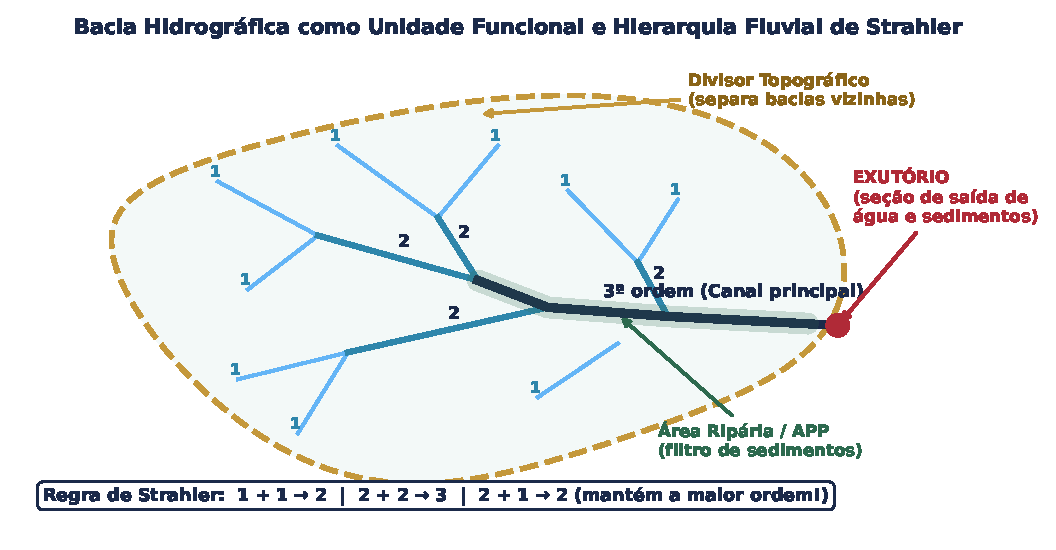
\includegraphics[width=0.92\textwidth]{figures/fig05_bacia_hidrografica_strahler.pdf}
  \caption{Elementos estruturais de uma bacia hidrográfica (divisor topográfico, áreas ripárias e exutório) e aplicação da Hierarquia Fluvial de Strahler até a 3ª ordem. Fonte: elaboração didática CHF662.}
  \label{fig:bacia_strahler}
\end{figure}

Além da ordem numérica, a geometria em planta da rede, denominada \textbf{padrão de drenagem}, revela o controle litológico e estrutural do terreno. O padrão \textbf{dendrítico (arborescente)} assemelha-se a galhos de árvore e ocorre em rochas de resistência homogênea, como granitos pouco fraturados ou camadas sedimentares horizontais. O padrão \textbf{retangular ou em treliça}, com confluências próximas a $90^\circ$, denuncia forte controle por falhas, fraturas ou dobramentos, sendo comum em setores serranos da Chapada Diamantina. Em encostas íngremes e uniformes desenvolve-se o padrão \textbf{paralelo}, com canais alongados, enquanto em morros isolados, domos ou depressões fechadas surge o padrão \textbf{radial}, divergente a partir do topo ou convergente para o centro da depressão.

O Exemplo 7.1 aplica passo a passo as três regras de Strahler a uma microbacia tributária do Rio Jacuípe.

\begin{boxExemplo}{7.1}{Hierarquia Fluvial de Strahler em uma Microbacia de Cabeceira (Básico)}
\passoEnunciado{Durante o mapeamento hidrográfico de uma microbacia afluente do Rio Jacuípe (BA), uma equipe identificou de montante para jusante sete córregos sem tributários ($C_1$ a $C_7$): $C_1$ e $C_2$ unem-se formando o trecho $T_1$; $C_3$ e $C_4$ unem-se formando $T_2$; $C_5$ desemboca em $T_2$, originando $T_3$; $T_1$ e $T_3$ encontram-se formando $T_4$; e $C_6$ e $C_7$ unem-se formando $T_5$, que desemboca em $T_4$ para gerar o canal principal $T_6$ até o exutório.}
\passoDados{Sete canais de cabeceira sem tributários ($C_1$ a $C_7$) e cinco confluências sequenciais até $T_6$.}
\passoPedido{Determinar a ordem de Strahler de cada trecho ($T_1$ a $T_6$) e a ordem final da microbacia.}
\passoMetodo{Aplicação sequencial das regras de Strahler (1952): nascentes $= 1$; encontro $n + n \to n + 1$; encontro $n + m \to \max(n, m)$.}
\passoContas{%
  Todos os sete canais sem afluentes ($C_1$ a $C_7$) pertencem à \textbf{1ª ordem}. Seguindo de montante para jusante, $T_1$ resulta de $C_1 + C_2$ ($1 + 1 \to \text{2ª ordem}$) e $T_2$ resulta de $C_3 + C_4$ ($1 + 1 \to \text{2ª ordem}$). Quando $C_5$ (1ª) encontra $T_2$ (2ª), prevalece a maior ordem em $T_3$ ($2 + 1 \to \text{2ª ordem}$). Na junção entre $T_1$ (2ª) e $T_3$ (2ª), a ordem sobe para \textbf{3ª ordem} em $T_4$ ($2 + 2 \to 3$). Na confluência seguinte, $T_5$ forma-se por $C_6 + C_7$ ($1 + 1 \to \text{2ª ordem}$) e desemboca em $T_4$ (3ª), mantendo $T_6$ na \textbf{3ª ordem} ($3 + 2 \to 3$).}
\passoResposta{$T_1 = 2^{\text{a}}$, $T_2 = 2^{\text{a}}$, $T_3 = 2^{\text{a}}$, $T_4 = 3^{\text{a}}$, $T_5 = 2^{\text{a}}$ e $T_6 = 3^{\text{a}}$ ordem, caracterizando uma \textbf{microbacia de 3ª ordem}.}
\passoVerificacao{Para surgir uma bacia de 4ª ordem seriam necessários ao menos dois canais de 3ª ordem confluindo entre si (exigindo no mínimo oito canais de 1ª ordem pareados); com sete canais de cabeceira, a 3ª ordem é o máximo possível.}
\end{boxExemplo}

Na aplicação dessa ordenação em mapas, o equívoco mais frequente consiste em somar ordens desiguais na confluência.

\begin{boxErro}[Erro 1: Somar Ordens Diferentes na Hierarquia de Strahler ($2 + 1 = 3$)]
\textbf{Equívoco frequente:} Assumir que toda confluência eleva a ordem fluvial, registrando que um canal de 2ª ordem ao receber um tributário de 1ª ordem passa a ser de 3ª ordem.\par
\textbf{Correção técnica:} Na regra de Strahler, a ordem só sobe quando confluem dois segmentos de mesma hierarquia ($1+1 \to 2$; $2+2 \to 3$). No encontro de ordens distintas, o trecho a jusante preserva a maior ordem ($2+1 \to 2$).
\end{boxErro}

\section{Morfometria de Bacias Hidrográficas}

A \textbf{análise morfométrica} traduz atributos geométricos, lineares, areais e hipsométricos da bacia em índices numéricos objetivos (Christofoletti, 1981; Villela; Mattos, 1975). Esses parâmetros permitem diagnosticar permeabilidade relativa do substrato, tempo de resposta às chuvas, suscetibilidade a enchentes e energia potencial para erosão.

\subsection{Densidade de Drenagem ($D_d$)}

Proposta por Robert E. Horton (1945), a \textbf{Densidade de Drenagem ($D_d$)} expressa o comprimento médio de canais fluviais por unidade de área da bacia, refletindo o balanço entre permeabilidade de solos e rochas, declividade, cobertura vegetal e regime pluviométrico. Em uma microbacia de área $A = 25{,}0\text{ km}^2$ e somatório dos canais $L_t = 45{,}0\text{ km}$, obtém-se $D_d = 45{,}0 / 25{,}0 = 1{,}80\text{ km}/\text{km}^2$, valor intermediário compatível com drenagem moderada.

\begin{boxFormula}[Equação da Densidade de Drenagem ($D_d$, Horton, 1945)]
\begin{align*}
  D_d &= \frac{L_t}{A}
\end{align*}
Aqui, $D_d$ é a densidade de drenagem ($\text{km}/\text{km}^2$ ou $\text{km}^{-1}$), $L_t$ representa o somatório do comprimento de todos os cursos d'água mapeados na bacia ($\text{km}$) e $A$ indica a área total de drenagem ($\text{km}^2$).
\end{boxFormula}

Valores baixos ($D_d < 0{,}5\text{ km}/\text{km}^2$) ocorrem em substratos muito permeáveis (como arenitos profundos e Latossolos arenosos) com elevada infiltração, enquanto valores altos ($D_d > 2{,}0\text{ km}/\text{km}^2$) predominam em rochas cristalinas pouco permeáveis e solos rasos do Semiárido sob chuvas concentradas. Como o comprimento $L_t$ depende da escala cartográfica e do limiar de área de contribuição adotado na extração automática em SIG, comparações entre bacias exigem redes vetorizadas na mesma escala e sob o mesmo critério. O Exemplo 7.2 ilustra esse contraste litológico em escala padronizada.

\begin{boxExemplo}{7.2}{Densidade de Drenagem e Contraste Litológico (Básico e Intermediário)}
\passoEnunciado{Em um diagnóstico comparativo na Bahia, analisaram-se duas microbacias rurais de mesma área, mapeadas na escala $1{:}25.000$: a \textbf{Microbacia A}, sobre embasamento cristalino (gnaisses) com solos rasos no Semiárido, e a \textbf{Microbacia B}, sobre bacia sedimentar arenosa com solos profundos e bem drenados.}
\passoDados{Microbacia A: $A_A = 16{,}0\text{ km}^2$ e $L_{tA} = 41{,}6\text{ km}$. Microbacia B: $A_B = 16{,}0\text{ km}^2$ e $L_{tB} = 12{,}8\text{ km}$.}
\passoPedido{Calcular a Densidade de Drenagem ($D_d$) de cada microbacia e explicar a relação entre os resultados, a permeabilidade do terreno e o escoamento superficial.}
\passoMetodo{Aplicação da equação de Horton ($D_d = L_t / A$) e razão comparativa $D_{dA}/D_{dB}$.}
\passoContas{%
  Calculando $D_d$ para as duas microbacias e comparando os valores obtidos:
  \begin{align*}
    D_{dA} &= \frac{41{,}6\text{ km}}{16{,}0\text{ km}^2} = 2{,}60\text{ km}/\text{km}^2 \\
    D_{dB} &= \frac{12{,}8\text{ km}}{16{,}0\text{ km}^2} = 0{,}80\text{ km}/\text{km}^2 \\
    \frac{D_{dA}}{D_{dB}} &= \frac{2{,}60}{0{,}80} = 3{,}25.
  \end{align*}}
\passoResposta{$D_{dA} = 2{,}60\text{ km}/\text{km}^2$ (drenagem alta) e $D_{dB} = 0{,}80\text{ km}/\text{km}^2$ (drenagem regular a baixa), sendo a densidade da Microbacia A $3{,}25$ vezes superior à da Microbacia B.}
\passoVerificacao{Rochas cristalinas e solos rasos limitam a infiltração profunda e exigem uma rede mais densa de canais para escoar a enxurrada, ao passo que arenitos e solos profundos favorecem a recarga subterrânea. Como ambas usaram a escala $1{:}25.000$, a comparação é válida.}
\end{boxExemplo}

\subsection{Índices de Forma: Coeficiente de Compacidade ($K_c$) e Índice de Circularidade ($I_c$)}

A geometria em planta da bacia controla a simultaneidade de chegada das ondas de cheia ao exutório. Em bacias próximas de um círculo, tributários distribuídos ao redor percorrem distâncias semelhantes até a saída, concentrando os picos de vazão, ao passo que bacias alongadas escalonam os tempos de viagem e atenuam o pico máximo, resposta que também depende da distribuição da chuva e da capacidade dos canais.

O \textbf{Coeficiente de Compacidade ($K_c$, Índice de Gravelius)} divide o perímetro real da bacia ($P$) pelo perímetro do círculo de mesma área ($P_c = 2\sqrt{\pi A}$), usando na prática hidrológica a constante $0{,}28$ (aproximação de $1/(2\sqrt{\pi}) \approx 0{,}2821$, que produz pequena diferença perto de $1$). Como nenhuma figura plana tem perímetro menor que o círculo de mesma área, tem-se sempre $K_c \ge 1$. De modo inverso, o \textbf{Índice de Circularidade ($I_c$, Miller, 1953)} divide a área real ($A$) pela área do círculo de mesmo perímetro ($A_c = P^2 / (4\pi)$), variando em $0 < I_c \le 1$ com $I_c \approx 1 / K_c^2$. Para a microbacia de $A = 25{,}0\text{ km}^2$ e $P = 24{,}0\text{ km}$, resultam $K_c = 0{,}28 \cdot (24{,}0 / 5{,}0) = 1{,}34$ e $I_c = (12{,}57 \times 25{,}0) / 576{,}0 \approx 0{,}55$, indicando contorno ovalado e suscetibilidade moderada a cheias.

\begin{boxFormula}[Equações de Forma: Compacidade ($K_c$) e Circularidade ($I_c$)]
\begin{align*}
  K_c &= \frac{P}{2\sqrt{\pi A}} \approx 0{,}28 \cdot \frac{P}{\sqrt{A}}, \qquad K_c \ge 1 \\[4pt]
  I_c &= \frac{4\pi \cdot A}{P^2} \approx \frac{12{,}57 \cdot A}{P^2}, \qquad 0 < I_c \le 1
\end{align*}
Em ambos os índices adimensionais, emprega-se $A$ em $\text{km}^2$ e $P$ em $\text{km}$ (ou $A$ em $\text{m}^2$ e $P$ em $\text{m}$). Quanto mais próximos de $1{,}0$ estão $K_c$ e $I_c$, mais circular é o contorno da bacia.
\end{boxFormula}

O Exemplo 7.3 aplica $K_c$ e $I_c$ à priorização de obras de macrodrenagem entre duas sub-bacias de mesma área.

\begin{boxExemplo}{7.3}{Forma da Bacia ($K_c$ e $I_c$) e Suscetibilidade a Enchentes (Intermediário)}
\passoEnunciado{A prefeitura de um município baiano precisa priorizar obras de macrodrenagem entre duas sub-bacias periurbanas de mesma área ($36{,}0\text{ km}^2$): a \textbf{Bacia X}, mais arredondada, e a \textbf{Bacia Y}, estreita e alongada.}
\passoDados{Bacia X: $A_X = 36{,}0\text{ km}^2$ e $P_X = 24{,}0\text{ km}$. Bacia Y: $A_Y = 36{,}0\text{ km}^2$ e $P_Y = 36{,}0\text{ km}$.}
\passoPedido{Calcular $K_c$ e $I_c$ de ambas as bacias e indicar qual apresenta maior suscetibilidade natural a picos rápidos de cheia.}
\passoMetodo{Cálculo de $K_c = 0{,}28 \cdot (P/\sqrt{A})$ e $I_c = (12{,}57 \cdot A)/P^2$, com classificação pela Tabela~\ref{tab:morfometria_interpretacao}.}
\passoContas{%
  Como $\sqrt{36{,}0} = 6{,}0\text{ km}$ em ambas as unidades, calculam-se os índices da Bacia X e da Bacia Y:
  \begin{align*}
    K_{cX} &= 0{,}28 \cdot \frac{24{,}0}{6{,}0} = 1{,}12, & I_{cX} &= \frac{12{,}57 \times 36{,}0}{24{,}0^2} \approx 0{,}79 \\
    K_{cY} &= 0{,}28 \cdot \frac{36{,}0}{6{,}0} = 1{,}68, & I_{cY} &= \frac{12{,}57 \times 36{,}0}{36{,}0^2} \approx 0{,}35.
  \end{align*}}
\passoResposta{Bacia X: $K_c = 1{,}12$ e $I_c = 0{,}79$ (contorno tendendo a circular, alta suscetibilidade a enchentes). Bacia Y: $K_c = 1{,}68$ e $I_c = 0{,}35$ (contorno alongado, baixa suscetibilidade a picos concentrados). A Bacia X deve receber prioridade.}
\passoVerificacao{Confere-se a consistência $1 / K_{cX}^2 = 1 / 1{,}12^2 \approx 0{,}80 \approx I_{cX}$, respeitando $K_c \ge 1$ e $I_c \le 1$.}
\end{boxExemplo}

Como $K_c$ e $I_c$ variam em direções opostas à medida que a bacia se alonga, confundir o sentido de leitura de ambos é erro comum em provas.

\begin{boxErro}[Erro 2: Confundir o Sentido de Interpretação de $K_c$ e $I_c$]
\textbf{Equívoco frequente:} Afirmar que ``quanto maior o $K_c$, mais circular é a bacia e maior o risco de enchentes'', confundindo $K_c$ com $I_c$.\par
\textbf{Correção técnica:} Os dois índices variam em sentidos opostos. Quanto mais circular a bacia, \textbf{menor} é $K_c$ (próximo de $1{,}0$) e \textbf{maior} é $I_c$ (próximo de $1{,}0$). Em bacias alongadas, $K_c$ cresce ($> 1{,}50$) e $I_c$ diminui ($< 0{,}45$). Valores com $K_c < 1$ ou $I_c > 1$ indicam erro de medição ou de cálculo.
\end{boxErro}

\subsection{Índices de Relevo: Amplitude Altimétrica ($H_m$) e Relação de Relevo ($R_r$)}

A energia potencial disponível para acelerar o escoamento e mobilizar sedimentos depende do desnível vertical combinado ao comprimento da bacia. A \textbf{Amplitude Altimétrica ($H_m$)} mede a diferença entre a cota máxima no divisor e a cota mínima no exutório, enquanto a \textbf{Relação de Relevo ($R_r$)}, proposta por Stanley Schumm (1956), divide esse desnível pelo comprimento axial ($L$). Na microbacia de referência com $H_{\max} = 420\text{ m}$, $H_{\min} = 220\text{ m}$ e $L = 8{,}0\text{ km}$, tem-se $H_m = 200\text{ m}$ e $R_r = 25{,}0\text{ m}/\text{km}$ ($0{,}025\text{ m}/\text{m}$ ou $2{,}5\%$).

\begin{boxFormula}[Equações de Relevo: Amplitude ($H_m$) e Relação de Relevo ($R_r$, Schumm, 1956)]
\begin{align*}
  H_m &= H_{\max} - H_{\min} \\[4pt]
  R_r &= \frac{H_m}{L}
\end{align*}
Aqui, $H_{\max}$ e $H_{\min}$ são as altitudes máxima e mínima ($\text{m}$), resultando em $H_m$ em metros ($\text{m}$), e $L$ é o comprimento axial da bacia ($\text{km}$ ou $\text{m}$). Expressa-se $R_r$ em $\text{m}/\text{km}$ (quando $L$ está em $\text{km}$) ou de forma adimensional em $\text{m}/\text{m}$ (convertendo $L$ para metros).
\end{boxFormula}

O Exemplo 7.4 compara duas cabeceiras baianas de mesmo comprimento axial e contrastante energia topográfica.

\begin{boxExemplo}{7.4}{Amplitude Altimétrica ($H_m$) e Relação de Relevo ($R_r$) em Cabeceiras Contrastantes (Intermediário)}
\passoEnunciado{Para avaliar o potencial energético de erosão e transporte de sedimentos, comparam-se duas microbacias de mesmo comprimento axial ($L = 6{,}0\text{ km}$): uma nas cabeceiras serranas da \textbf{Chapada Diamantina} e outra em setor aplainado do \textbf{Planalto Sertanejo}.}
\passoDados{Chapada Diamantina: $H_{\max} = 960\text{ m}$, $H_{\min} = 480\text{ m}$, $L = 6{,}0\text{ km}$. Planalto Sertanejo: $H_{\max} = 360\text{ m}$, $H_{\min} = 240\text{ m}$, $L = 6{,}0\text{ km}$.}
\passoPedido{Calcular $H_m$ e $R_r$ (em $\text{m}/\text{km}$ e em $\text{m}/\text{m}$) para ambas as unidades e interpretar suas implicações geomorfológicas.}
\passoMetodo{Aplicação de $H_m = H_{\max} - H_{\min}$ e $R_r = H_m / L$, convertendo $6{,}0\text{ km} = 6.000\text{ m}$ para a forma adimensional.}
\passoContas{%
  Calculando amplitude e relação de relevo para a Chapada Diamantina (1) e para o Planalto Sertanejo (2):
  \begin{align*}
    H_{m1} &= 960 - 480 = 480\text{ m}, & R_{r1} &= \frac{480}{6{,}0} = 80{,}0\text{ m}/\text{km} \quad \left(\frac{480}{6.000} = 0{,}080\text{ m}/\text{m}\right) \\
    H_{m2} &= 360 - 240 = 120\text{ m}, & R_{r2} &= \frac{120}{6{,}0} = 20{,}0\text{ m}/\text{km} \quad \left(\frac{120}{6.000} = 0{,}020\text{ m}/\text{m}\right).
  \end{align*}}
\passoResposta{Chapada Diamantina: $H_m = 480\text{ m}$ e $R_r = 80{,}0\text{ m}/\text{km}$ ($0{,}080\text{ m}/\text{m}$). Planalto Sertanejo: $H_m = 120\text{ m}$ e $R_r = 20{,}0\text{ m}/\text{km}$ ($0{,}020\text{ m}/\text{m}$). A microbacia serrana possui energia de relevo $4$ vezes maior.}
\passoVerificacao{O mesmo comprimento axial acomoda um desnível quatro vezes superior na Chapada, elevando a velocidade do escoamento, a competência para transportar material grosseiro e a suscetibilidade a ravinas caso haja supressão vegetal.}
\end{boxExemplo}

A compatibilidade de unidades no denominador de $R_r$ exige atenção constante para evitar discrepâncias de mil vezes no resultado numérico.

\begin{boxErro}[Erro 3: Misturar Metros e Quilômetros no Cálculo da Relação de Relevo ($R_r$)]
\textbf{Equívoco frequente:} Dividir $H_m = 200\text{ m}$ por $L = 8\text{ km}$, obter $25$ e registrar o valor como ``$25\text{ m/m}$'' ou ``$25\%$''.\par
\textbf{Correção técnica:} Ao dividir metros por quilômetros, a unidade obrigatória é $\text{m}/\text{km}$ ($25\text{ m}/\text{km}$). Para obter $R_r$ adimensional ($\text{m}/\text{m}$) ou em porcentagem, converta $L$ para metros antes da divisão: $200\text{ m} / 8.000\text{ m} = 0{,}025\text{ m}/\text{m} = 2{,}5\%$.
\end{boxErro}

Para apoiar a leitura comparativa desses parâmetros em diagnósticos ambientais, a Tabela~\ref{tab:morfometria_interpretacao} reúne as faixas de referência usuais, que devem ser sempre interpretadas em conjunto com litologia, solos, cobertura e regime pluviométrico.

\begin{table}[H]
\centering
\caption{Síntese interpretativa dos principais índices morfométricos de bacias hidrográficas.}
\label{tab:morfometria_interpretacao}
\renewcommand{\arraystretch}{1.20}
\small
\begin{tabularx}{\textwidth}{@{}p{2.7cm} p{3.1cm} >{\raggedright\arraybackslash}X@{}}
  \toprule
  \rowcolor{uefsNavy}
  \textcolor{white}{\bfseries Índice} & \textcolor{white}{\bfseries Faixa de Valores} & \textcolor{white}{\bfseries Significado Hidrológico e Ambiental} \\
  \midrule
  \multirow{3}{2.7cm}{\textbf{Densidade de Drenagem ($D_d$)}} & $< 0{,}5\text{ km}/\text{km}^2$ & Drenagem pobre; substrato muito permeável e alta infiltração. \\
  & $0{,}5\text{ a } 2{,}0\text{ km}/\text{km}^2$ & Drenagem regular a média; equilíbrio intermediário. \\
  & $> 2{,}0\text{ km}/\text{km}^2$ & Drenagem alta; substrato pouco permeável e maior dissecação. \\
  \midrule
  \rowcolor{bgGray}
  \multirow{3}{2.7cm}{\textbf{Compacidade ($K_c$)}} & $1{,}00\text{ a } 1{,}25$ & Contorno circular; alta propensão a picos rápidos de cheia. \\
  \rowcolor{bgGray}
  & $1{,}25\text{ a } 1{,}50$ & Contorno ovalado; propensão moderada a cheias. \\
  \rowcolor{bgGray}
  & $> 1{,}50$ & Contorno alongado; menor concentração simultânea de picos. \\
  \midrule
  \multirow{2}{2.7cm}{\textbf{Circularidade ($I_c$)}} & $> 0{,}51$ & Tendência circular; convergência rápida ao exutório. \\
  & $\le 0{,}51$ & Tendência alongada; escoamento distribuído no tempo. \\
  \midrule
  \rowcolor{bgGray}
  \multirow{2}{2.7cm}{\textbf{Relação de Relevo ($R_r$)}} & $< 15\text{ m}/\text{km}$ & Relevo suave; menor velocidade e tendência à deposição. \\
  \rowcolor{bgGray}
  & $> 40\text{ m}/\text{km}$ & Relevo acidentado; alta energia erosiva e de transporte. \\
  \bottomrule
\end{tabularx}
\end{table}

\section{Áreas Ripárias, Conectividade Hidrossedimentológica e Uso da Terra}

Os índices morfométricos descrevem a arquitetura física de evolução lenta da bacia, mas a resposta hidrológica real depende criticamente da cobertura vegetal nas vertentes e nas margens fluviais.

\subsection{Áreas Ripárias e Zonas Tampão}

As \textbf{áreas ripárias} (matas ciliares, galerias e várzeas marginais, protegidas como Áreas de Preservação Permanente pelo Código Florestal, Lei nº 12.651/2012) constituem a interface entre a vertente e o canal fluvial. Quando a enxurrada desce a encosta e atravessa uma faixa ripária conservada, a serapilheira e os caules aumentam a rugosidade superficial, dissipam a energia cinética do fluxo e retêm sedimentos e agroquímicos antes que atinjam o rio. Simultaneamente, o entrelaçamento das raízes eleva a resistência ao cisalhamento dos barrancos e contém o solapamento das margens, enquanto o sombreamento regula a temperatura da água e os solos porosos mantêm a recarga que sustenta o fluxo de base nas estiagens.

Quando a vegetação ciliar é suprimida em uma das margens ou em ambas, perde-se essa zona tampão filtrante e estabilizadora: o solo exposto sofre desagregação rápida e os sedimentos carreados depositam-se no leito fluvial, reduzindo a profundidade da calha e ampliando o assoreamento (Figura~\ref{fig:assoreamento_mata_ciliar}).

\begin{figure}[H]
  \centering
  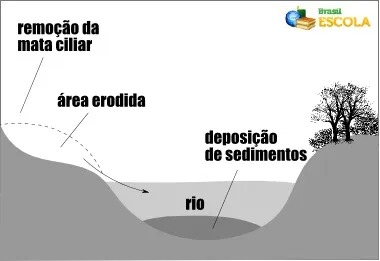
\includegraphics[width=0.72\textwidth]{figures/assoreamento_2.jpg}
  \caption{Esquema didático da remoção de mata ciliar, erosão marginal e deposição de sedimentos no leito fluvial (assoreamento). Fonte: acervo didático da disciplina.}
  \label{fig:assoreamento_mata_ciliar}
\end{figure}

\subsection{Conectividade Hidrossedimentológica}

Na geomorfologia fluvial, denomina-se \textbf{conectividade hidrossedimentológica} a eficiência com que água e sedimentos mobilizados nas vertentes alcançam a rede de canais e o exutório (Brierley; Fryirs, 2005). A \textbf{conectividade estrutural} diz respeito à continuidade física dos caminhos de fluxo no relevo (declividade, ravinas, estradas rurais mal drenadas ou galerias pluviais), enquanto a \textbf{conectividade funcional} expressa a ativação efetiva desses caminhos durante eventos chuvosos, como ocorre em canais efêmeros do Semiárido que permanecem secos na maior parte do ano e conectam-se apenas quando chuvas convectivas superam a infiltração do solo. Faixas ciliares conservadas, terraços em nível e paliçadas operam como \textbf{desconectores}, ao passo que estradas morro abaixo atuam como \textbf{conectores artificiais}.

\subsection{Impactos da Mudança de Uso da Terra: Impermeabilização e Desmatamento}

A conversão de florestas ou Caatinga conservada em pastagens compactadas ou loteamentos urbanos impermeabilizados altera profundamente o balanço hídrico da microbacia. A perda de dossel e a selagem por asfalto, telhados e solos adensados derrubam a interceptação e a infiltração, elevando o \textbf{coeficiente de escoamento superficial ($C$)} de valores típicos entre $0{,}10$ e $0{,}20$ em coberturas florestais para $0{,}65$ a $0{,}90$ em áreas urbanas densas.

Como resultado, a água escoa mais rápido pela superfície, reduz o \textbf{tempo de concentração} e gera hidrogramas com picos de cheia mais elevados e precoces sob a mesma chuva (cenário recorrente em microbacias urbanizadas de Feira de Santana, como nas cabeceiras do Subaé e do Jacuípe), enquanto a redução da infiltração diminui a recarga dos aquíferos e deprime o fluxo de base na estiagem, dinâmica contrastada com a leitura física de $D_d$, $K_c$ e $I_c$ na Figura~\ref{fig:hidrograma_impermeabilizacao}.

\begin{figure}[H]
  \centering
  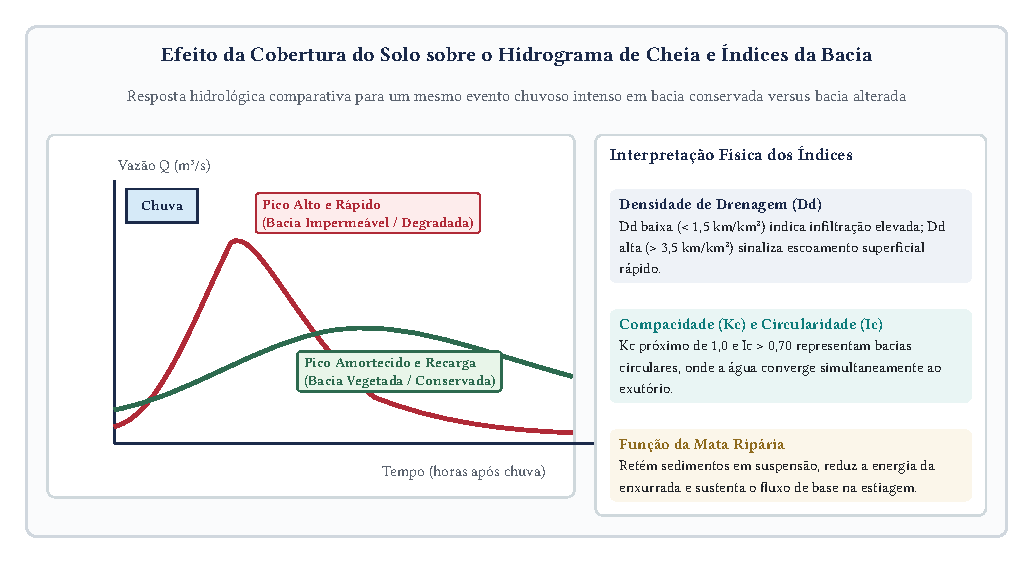
\includegraphics[width=0.95\textwidth]{figures/fig_cap07_hidrograma_impermeabilizacao.pdf}
  \caption{Comparação entre hidrogramas de cheia em bacia vegetada e bacia impermeabilizada sob mesmo evento chuvoso, articulada à interpretação física de $D_d$, $K_c$, $I_c$ e da mata ripária. Fonte: elaboração didática CHF662.}
  \label{fig:hidrograma_impermeabilizacao}
\end{figure}

% ============================================================================
% ETAPA 4 — ESTUDO DE CASO AVANÇADO (EXEMPLO 7.5)
% ============================================================================
\etapa{4}{Síntese Aplicada em Hidrologia de Microbacias}

A comparação gráfica dos hidrogramas na Figura~\ref{fig:hidrograma_impermeabilizacao} traduz-se diretamente em volumes escoados durante uma tormenta. Multiplicar a lâmina precipitada pela área da microbacia e pelo coeficiente de escoamento superficial ($C$) permite quantificar o incremento de enxurrada gerado pela urbanização sem drenagem sustentável, como desenvolvido no Exemplo 7.5.

\begin{boxExemplo}{7.5}{Impacto Hidrológico da Impermeabilização Urbana em uma Microbacia (Avançado)}
\passoEnunciado{Uma microbacia periurbana de $4{,}0\text{ km}^2$ na borda de expansão de Feira de Santana era originalmente coberta por vegetação nativa e áreas ripárias conservadas, com coeficiente médio de escoamento superficial $C_1 = 0{,}15$. Após loteamentos pavimentados, canalização de córregos e supressão da mata ciliar, o coeficiente subiu para $C_2 = 0{,}75$. Considere uma chuva intensa de $P_{\text{chuva}} = 60\text{ mm}$.}
\passoDados{$A = 4{,}0\text{ km}^2 = 4.000.000\text{ m}^2$; $P_{\text{chuva}} = 60\text{ mm} = 0{,}060\text{ m}$; $C_1 = 0{,}15$; $C_2 = 0{,}75$.}
\passoPedido{Calcular o volume total precipitado, o volume de escoamento superficial antes e depois da urbanização, a diferença absoluta e relativa e os reflexos sobre a conectividade hidrossedimentológica.}
\passoMetodo{Cálculo volumétrico do balanço superficial ($V_{\text{prec}} = P_{\text{chuva}} \cdot A$ e $V_{\text{esc}} = C \cdot V_{\text{prec}}$), seguido de análise hidrossedimentológica.}
\passoContas{%
  Convertendo $A = 4.000.000\text{ m}^2$ e $P_{\text{chuva}} = 0{,}060\text{ m}$, obtêm-se os volumes precipitado, escoados e o incremento relativo:
  \begin{align*}
    V_{\text{prec}} &= 0{,}060\text{ m} \times 4.000.000\text{ m}^2 = 240.000\text{ m}^3 \\
    V_{\text{esc},1} &= 0{,}15 \times 240.000\text{ m}^3 = 36.000\text{ m}^3 \\
    V_{\text{esc},2} &= 0{,}75 \times 240.000\text{ m}^3 = 180.000\text{ m}^3 \\
    \Delta V_{\text{esc}} &= 180.000 - 36.000 = 144.000\text{ m}^3 \qquad \left(\frac{180.000}{36.000} = 5\text{ vezes, ou }+400\%\right).
  \end{align*}
  No cenário conservado, os $204.000\text{ m}^3$ restantes ($85\%$) permaneciam retidos por interceptação, depressões e infiltração.}
\passoResposta{O escoamento superficial saltou de $36.000\text{ m}^3$ para $180.000\text{ m}^3$, um acréscimo de $144.000\text{ m}^3$ (cinco vezes o volume original) para a mesma chuva de $60\text{ mm}$.}
\passoVerificacao{Esse acréscimo equivale a cerca de $58$ piscinas olímpicas ($2.500\text{ m}^3$ cada) lançadas abruptamente no canal em poucas horas. A supressão da mata ciliar e a canalização eliminam os desconectores naturais, amplificam a conectividade artificial e provocam alagamentos a jusante, erosão marginal e queda na recarga subterrânea.}
\end{boxExemplo}

% ============================================================================
% ETAPA 5 — ERRO 4 E MATERIAIS AUDIOVISUAIS DE APOIO
% ============================================================================
\etapa{5}{Armadilha Conceitual e Materiais Audiovisuais de Apoio}

Mesmo quando os índices morfométricos são calculados corretamente nas fórmulas de Horton, Gravelius e Miller, comparar bacias vetorizadas em escalas cartográficas incompatíveis invalida qualquer conclusão sobre permeabilidade e dissecação.

\begin{boxErro}[Erro 4: Comparar Densidade de Drenagem ($D_d$) Obtida em Escalas Cartográficas Diferentes]
\textbf{Equívoco frequente:} Calcular $D_d$ de uma bacia sobre base $1{:}10.000$ e compará-la com o $D_d$ de outra bacia extraído de carta $1{:}100.000$, concluindo que a primeira apresenta substrato muito menos permeável.\par
\textbf{Correção técnica:} Cartas de pequena escala ($1{:}100.000$) generalizam a rede hidrográfica e omitem grande parte dos canais de 1ª ordem, subestimando $L_t$ e $D_d$. Comparações morfométricas válidas exigem vetorização na mesma escala e sob o mesmo critério de extração de canais.
\end{boxErro}

Para aprofundar a compreensão da bacia hidrográfica como unidade de gestão e dos processos erosivos em rede de drenagem, assista às videoaulas selecionadas na página da disciplina: \textit{Gestão de Recursos Hídricos} (\url{https://www.youtube.com/watch?v=odVchJ9pmgY}), que aborda a bacia hidrográfica na análise ambiental integrada e na Lei das Águas, e \textit{Processos Erosivos e Relevo} (\url{https://www.youtube.com/watch?v=G6Q0iU_n6xI}), dedicada à dinâmica de escoamento e morfogênese nas vertentes e canais.

% ============================================================================
% ETAPA 6 — EXERCÍCIOS DE FIXAÇÃO
% ============================================================================
\etapa{6}{Exercícios de Fixação}

\subsection*{Nível Básico (Exercícios 1 a 5)}

\begin{enumerate}[leftmargin=1.8em, itemsep=4pt]
  \item Explique, com base em Botelho e Silva (2004) e Christofoletti (1981), por que a bacia hidrográfica é considerada a unidade espacial mais adequada para a análise e o planejamento ambiental, diferenciando \textbf{divisor topográfico}, \textbf{talvegue} e \textbf{exutório}.
  \espacoResolucao[2.0cm]

  \item Uma microbacia rural apresenta área de drenagem $A = 20{,}0\text{ km}^2$ e comprimento total de canais $L_t = 35{,}0\text{ km}$. Calcule sua Densidade de Drenagem ($D_d$) e classifique-a conforme a Tabela~\ref{tab:morfometria_interpretacao}.
  \espacoResolucao[1.8cm]

  \item Calcule o Coeficiente de Compacidade ($K_c$) de uma sub-bacia com área $A = 49{,}0\text{ km}^2$ e perímetro $P = 35{,}0\text{ km}$. Indique se sua forma tende à circular, ovalada ou alongada.
  \espacoResolucao[1.8cm]

  \item Uma microbacia possui área $A = 25{,}0\text{ km}^2$ e perímetro $P = 25{,}0\text{ km}$. Calcule seu Índice de Circularidade ($I_c$) e avalie sua propensão natural a picos concentrados de enchente.
  \espacoResolucao[1.8cm]

  \item Determine a Amplitude Altimétrica ($H_m$) e a Relação de Relevo ($R_r$), em $\text{m}/\text{km}$ e em $\text{m}/\text{m}$, para uma bacia com $H_{\max} = 640\text{ m}$, $H_{\min} = 280\text{ m}$ e comprimento axial $L = 9{,}0\text{ km}$.
  \espacoResolucao[1.8cm]
\end{enumerate}

\subsection*{Nível Intermediário (Exercícios 6 a 10)}

\begin{enumerate}[leftmargin=1.8em, itemsep=4pt, resume]
  \item Compare duas bacias hidrográficas mapeadas na mesma escala ($1{:}25.000$), ambas com área $A = 64{,}0\text{ km}^2$:
  \begin{itemize}[leftmargin=1.4em, itemsep=1pt]
    \item \textbf{Bacia M1:} $P = 32{,}0\text{ km}$, $L_t = 160{,}0\text{ km}$, $H_{\max} = 540\text{ m}$, $H_{\min} = 220\text{ m}$, $L = 8{,}0\text{ km}$.
    \item \textbf{Bacia M2:} $P = 48{,}0\text{ km}$, $L_t = 51{,}2\text{ km}$, $H_{\max} = 380\text{ m}$, $H_{\min} = 220\text{ m}$, $L = 16{,}0\text{ km}$.
  \end{itemize}
  Calcule $D_d$, $K_c$, $I_c$, $H_m$ e $R_r$ para ambas e justifique qual delas exige maior cuidado contra cheias rápidas e processos erosivos.
  \espacoResolucao[2.6cm]

  \item Em uma rede hidrográfica hipotética, quatro pares de canais de 1ª ordem formam quatro canais de 2ª ordem ($A, B, C, D$). Os canais $A$ e $B$ se unem formando o trecho $X$; o canal $C$ desemboca em $X$ formando o trecho $Y$; e o canal $D$ desemboca em $Y$ formando o canal final $Z$ no exutório. Determine a ordem de Strahler de $X$, $Y$ e $Z$ e explique por que a ordem final não chegou a 4ª ordem.
  \espacoResolucao[2.0cm]

  \item Uma microbacia de $5{,}0\text{ km}^2$ sofreu desmatamento e abertura de estradas compactadas, elevando seu coeficiente de escoamento superficial de $C_1 = 0{,}20$ para $C_2 = 0{,}70$. Para uma chuva de $50\text{ mm}$, calcule o volume escoado superficialmente (em $\text{m}^3$) nos dois cenários e o percentual de aumento do escoamento.
  \espacoResolucao[2.2cm]

  \item Explique a diferença entre \textbf{conectividade estrutural} e \textbf{conectividade funcional} em uma bacia hidrográfica do Semiárido baiano e dê um exemplo de elemento que atua como \textit{conector} e outro que atua como \textit{desconector} de sedimentos.
  \espacoResolucao[2.0cm]

  \item Por que a supressão de matas ciliares (áreas ripárias) em microbacias rurais provoca simultaneamente aumento da turbidez da água, assoreamento de reservatórios e instabilidade de margens?
  \espacoResolucao[2.0cm]
\end{enumerate}

\subsection*{Questões Objetivas (Exercícios 11 a 15)}

\begin{enumerate}[leftmargin=1.8em, itemsep=5pt, resume]
  \item Na Hierarquia Fluvial de Strahler, quando um curso d'água de 3ª ordem recebe um afluente de 2ª ordem e, mais a jusante, conflui com outro curso d'água de 3ª ordem, as ordens dos segmentos imediatamente após a primeira e a segunda confluência serão, respectivamente:
  \begin{alternativas}
    \item 4ª ordem e 5ª ordem.
    \item 3ª ordem e 4ª ordem.
    \item 3ª ordem e 3ª ordem.
    \item 5ª ordem e 6ª ordem.
    \item 2ª ordem e 4ª ordem.
  \end{alternativas}

  \item Uma bacia hidrográfica apresenta $A = 100{,}0\text{ km}^2$, $P = 50{,}0\text{ km}$, $L_t = 220{,}0\text{ km}$, $H_{\max} = 750\text{ m}$, $H_{\min} = 250\text{ m}$ e $L = 20{,}0\text{ km}$. Os valores corretos de $D_d$, $K_c$ e $R_r$ (em $\text{m}/\text{km}$) são, respectivamente:
  \begin{alternativas}
    \item $2{,}20\text{ km}/\text{km}^2$; $1{,}40$; $25{,}0\text{ m}/\text{km}$.
    \item $0{,}45\text{ km}/\text{km}^2$; $1{,}40$; $25{,}0\text{ m}/\text{km}$.
    \item $2{,}20\text{ km}/\text{km}^2$; $0{,}71$; $50{,}0\text{ m}/\text{km}$.
    \item $2{,}20\text{ km}/\text{km}^2$; $1{,}40$; $0{,}25\text{ m}/\text{km}$.
    \item $4{,}40\text{ km}/\text{km}^2$; $2{,}80$; $25{,}0\text{ m}/\text{km}$.
  \end{alternativas}

  \item Sobre o Coeficiente de Compacidade ($K_c$) e o Índice de Circularidade ($I_c$), assinale a alternativa tecnicamente correta:
  \begin{alternativas}
    \item Uma bacia perfeitamente circular apresenta $K_c = 0$ e $I_c = 1$.
    \item Quanto maior o valor de $K_c$, maior a tendência da bacia à forma circular e maior o risco de cheias súbitas.
    \item Valores de $K_c$ próximos de $1{,}0$ e de $I_c$ próximos de $1{,}0$ indicam bacia mais circular e maior suscetibilidade a picos concentrados de enchente.
    \item O valor de $I_c$ pode assumir qualquer número real positivo superior a $1{,}0$ em bacias muito alongadas.
    \item Os índices $K_c$ e $I_c$ dependem exclusivamente da altitude máxima e da extensão dos rios, independendo do perímetro.
  \end{alternativas}

  \item Em relação às áreas ripárias em bacias hidrográficas, é \textbf{INCORRETO} afirmar que:
  \begin{alternativas}
    \item Atuam como zonas tampão que retêm parte dos sedimentos e nutrientes carreados das vertentes.
    \item Contribuem para a estabilização das margens fluviais por meio do sistema radicular da vegetação.
    \item Aumentam a rugosidade superficial, reduzindo a velocidade do escoamento que alcança o canal.
    \item Sua remoção eleva a conectividade hidrossedimentológica entre encostas agrícolas e o leito fluvial.
    \item Sua supressão aumenta a recarga dos aquíferos locais ao eliminar o consumo de água por evapotranspiração.
  \end{alternativas}

  \item A urbanização intensa e sem drenagem sustentável em uma microbacia provoca, no hidrograma de cheia medido no exutório:
  \begin{alternativas}
    \item Aumento do tempo de concentração e diminuição do pico de vazão.
    \item Redução do volume escoado superficialmente e elevação do fluxo de base na estiagem.
    \item Redução do tempo de concentração e aumento acentuado da vazão de pico.
    \item Manutenção inalterada da curva de cheia, pois a área da bacia permanece constante.
    \item Eliminação da conectividade estrutural entre vertentes e canais.
  \end{alternativas}
\end{enumerate}

\etapa{7}{Questões de Provas, ENADE e Concursos Ambientais}

\begin{enumerate}[leftmargin=1.8em, itemsep=5pt, start=16]
  \item \textbf{(Questão autoral, estilo ENADE / Licenciatura e Bacharelado em Geografia)} Um órgão estadual de meio ambiente avalia o pedido de supressão vegetal para expansão agropecuária em uma microbacia de cabeceira situada sobre embasamento cristalino no Nordeste brasileiro. O relatório técnico apresentou $D_d = 2{,}85\text{ km}/\text{km}^2$, $K_c = 1{,}14$ e $R_r = 55\text{ m}/\text{km}$. Com base na interpretação integrada desses indicadores morfométricos, conclui-se que a microbacia apresenta:
  \begin{alternativas}
    \item Substrato muito permeável, forma alongada e relevo plano, com baixíssima vulnerabilidade à erosão hídrica.
    \item Elevada capacidade de infiltração profunda e lenta resposta hidrológica, dispensando faixas ripárias protetoras.
    \item Baixa permeabilidade relativa, forma tendente à circular e elevada energia de relevo, indicando alta propensão natural a enxurradas rápidas e processos erosivos caso a vegetação seja suprimida.
    \item Predomínio de deposição sedimentar em planície aluvial ampla, pois $K_c$ próximo de $1{,}0$ impede a concentração do escoamento no exutório.
    \item Incompatibilidade matemática nos dados, visto que uma bacia com $D_d > 2{,}0$ não pode apresentar $K_c > 1{,}0$.
  \end{alternativas}

  \item \textbf{(Questão autoral, estilo Concurso Analista Ambiental / INEMA-BA)} Em um estudo hidrológico para outorga e prevenção de inundações, uma sub-bacia foi caracterizada por $A = 81{,}0\text{ km}^2$, $P = 36{,}0\text{ km}$, $L_t = 202{,}5\text{ km}$, $H_{\max} = 680\text{ m}$, $H_{\min} = 230\text{ m}$ e $L = 15{,}0\text{ km}$. Assinale a alternativa que apresenta corretamente os valores de $D_d$, $K_c$, $I_c$ e $R_r$ (em $\text{m}/\text{m}$) dessa sub-bacia:
  \begin{alternativas}
    \item $D_d = 2{,}50\text{ km}/\text{km}^2$; $K_c = 1{,}12$; $I_c = 0{,}79$; $R_r = 0{,}030\text{ m}/\text{m}$.
    \item $D_d = 2{,}50\text{ km}/\text{km}^2$; $K_c = 1{,}12$; $I_c = 0{,}79$; $R_r = 30{,}0\text{ m}/\text{m}$.
    \item $D_d = 0{,}40\text{ km}/\text{km}^2$; $K_c = 1{,}12$; $I_c = 0{,}79$; $R_r = 0{,}030\text{ m}/\text{m}$.
    \item $D_d = 2{,}50\text{ km}/\text{km}^2$; $K_c = 1{,}40$; $I_c = 0{,}50$; $R_r = 0{,}030\text{ m}/\text{m}$.
    \item $D_d = 2{,}50\text{ km}/\text{km}^2$; $K_c = 0{,}89$; $I_c = 1{,}26$; $R_r = 0{,}030\text{ m}/\text{m}$.
  \end{alternativas}

  \item \textbf{(Questão autoral, estilo Concurso IBAMA / Gestão de Bacias Hidrográficas)} Sobre o conceito de conectividade hidrossedimentológica aplicado à gestão de bacias hidrográficas, analise as afirmativas abaixo:
  \begin{itemize}[leftmargin=1.4em, itemsep=1.5pt]
    \item[I.] Estradas vicinais não pavimentadas construídas no sentido da declividade atuam como conectores estruturais, canalizando o escoamento das vertentes diretamente para os cursos d'água.
    \item[II.] A recomposição de matas ciliares e a implantação de barreiras de retenção de sedimentos reduzem a conectividade entre áreas degradadas e o canal principal.
    \item[III.] Em climas semiáridos, canais efêmeros podem exibir alta conectividade estrutural em mapa, mas conectividade funcional intermitente, ativada apenas em eventos pluviométricos que superam a capacidade de infiltração.
  \end{itemize}
  Está correto o que se afirma em:
  \begin{alternativas}
    \item I, apenas.
    \item II, apenas.
    \item I e II, apenas.
    \item II e III, apenas.
    \item I, II e III.
  \end{alternativas}
\end{enumerate}

\begin{boxDica}[Conexão com a Avaliação Teórica e com o Trabalho Prático Final]
Na \textbf{Prova Teórica da Semana 10}, os índices morfométricos exigem calcular ($D_d$, $K_c$, $I_c$ e $R_r$) e interpretar o comportamento físico de cada valor. No \textbf{Trabalho Prático Final}, extrair esses cinco índices em SIG (QGIS) para a microbacia escolhida, documentando a escala e o critério de extração da rede, confere precisão técnica à caracterização da área de estudo.
\end{boxDica}

\clearpage
\etapa{8}{Gabarito Comentado: Exercícios 1 a 18}

\begin{boxGabarito}[Resoluções e Justificativas: Capítulo 7]
\begin{enumerate}[leftmargin=1.8em, itemsep=3.5pt]
  \item \textbf{Conceito e elementos:} a bacia hidrográfica é uma unidade espacial natural e sistêmica na qual todos os fluxos de água, sedimentos e poluentes das vertentes convergem para um único exutório, permitindo relacionar diretamente o uso da terra ao estado dos recursos hídricos (Botelho; Silva, 2004; Christofoletti, 1981). \textit{Divisor topográfico}: linha de pontos mais altos que separa bacias adjacentes; \textit{talvegue}: linha de pontos mais baixos ao longo do vale onde se aloja o canal; \textit{exutório}: ponto de menor cota do contorno por onde sai toda a drenagem superficial.

  \item \textbf{Cálculo de $D_d$:} $D_d = L_t / A = 35{,}0 / 20{,}0 = \mathbf{1{,}75\text{ km}/\text{km}^2}$. Classificação: drenagem regular a média ($0{,}5$ a $2{,}0\text{ km}/\text{km}^2$).

  \item \textbf{Cálculo de $K_c$:} $\sqrt{49{,}0} = 7{,}0\text{ km}$. Logo, $K_c = 0{,}28 \cdot (35{,}0 / 7{,}0) = 0{,}28 \cdot 5{,}0 = \mathbf{1{,}40}$. Classificação: forma ovalada ($1{,}25$ a $1{,}50$), suscetibilidade moderada a cheias.

  \item \textbf{Cálculo de $I_c$:} $I_c = \frac{12{,}57 \cdot 25{,}0}{(25{,}0)^2} = \frac{12{,}57}{25{,}0} = \mathbf{0{,}5028 \approx 0{,}50}$. Por situar-se no limiar de $0{,}51$, indica forma intermediária (levemente alongada/ovalada), com propensão moderada a cheias concentradas.

  \item \textbf{Cálculo de $H_m$ e $R_r$:} $H_m = 640 - 280 = \mathbf{360\text{ m}}$. Em $\text{m}/\text{km}$: $R_r = 360 / 9{,}0 = \mathbf{40{,}0\text{ m}/\text{km}}$. Em $\text{m}/\text{m}$: $L = 9{,}0\text{ km} = 9.000\text{ m} \Rightarrow R_r = 360 / 9.000 = \mathbf{0{,}040\text{ m}/\text{m}}$ ($4{,}0\%$).

  \item \textbf{Comparação M1 vs. M2:} como $\sqrt{64{,}0} = 8{,}0$:
  \begin{itemize}[leftmargin=1.4em, itemsep=1pt]
    \item \textbf{M1:} $D_d = 160{,}0 / 64{,}0 = \mathbf{2{,}50\text{ km}/\text{km}^2}$; $K_c = 0{,}28 \cdot (32{,}0 / 8{,}0) = \mathbf{1{,}12}$; $I_c = 12{,}57 \cdot 64{,}0 / 32{,}0^2 = 804{,}48 / 1.024 = \mathbf{0{,}79}$; $H_m = 540 - 220 = \mathbf{320\text{ m}}$; $R_r = 320 / 8{,}0 = \mathbf{40{,}0\text{ m}/\text{km}}$ ($0{,}040\text{ m}/\text{m}$).
    \item \textbf{M2:} $D_d = 51{,}2 / 64{,}0 = \mathbf{0{,}80\text{ km}/\text{km}^2}$; $K_c = 0{,}28 \cdot (48{,}0 / 8{,}0) = \mathbf{1{,}68}$; $I_c = 12{,}57 \cdot 64{,}0 / 48{,}0^2 = 804{,}48 / 2.304 = \mathbf{0{,}35}$; $H_m = 380 - 220 = \mathbf{160\text{ m}}$; $R_r = 160 / 16{,}0 = \mathbf{10{,}0\text{ m}/\text{km}}$ ($0{,}010\text{ m}/\text{m}$).
  \end{itemize}
  \textbf{Conclusão:} a \textbf{Bacia M1} exige muito maior cuidado contra cheias rápidas e erosão, pois combina alta densidade de drenagem ($2{,}50$), contorno tendente ao circular ($K_c = 1{,}12$; $I_c = 0{,}79$) e energia de relevo quatro vezes superior ($40{,}0$ contra $10{,}0\text{ m}/\text{km}$).

  \item \textbf{Hierarquia de Strahler:} $A$ (2ª) $+ B$ (2ª) $\to X$ (\textbf{3ª ordem}). Em seguida, $X$ (3ª) $+ C$ (2ª) $\to Y$ (\textbf{3ª ordem}, pois $3 > 2$). Depois, $Y$ (3ª) $+ D$ (2ª) $\to Z$ (\textbf{3ª ordem}). A bacia permaneceu na 3ª ordem porque $C$ e $D$ desembocaram separadamente no canal de 3ª ordem; para surgir uma 4ª ordem, $C$ e $D$ precisariam ter confluído entre si formando um segundo canal de 3ª ordem antes de encontrar $X$.

  \item \textbf{Balanço do escoamento:} $A = 5{,}0\text{ km}^2 = 5.000.000\text{ m}^2$; $P_{\text{chuva}} = 50\text{ mm} = 0{,}050\text{ m}$. Volume precipitado: $V_{\text{prec}} = 0{,}050 \times 5.000.000 = 250.000\text{ m}^3$. Antes ($C_1 = 0{,}20$): $V_1 = 0{,}20 \times 250.000 = \mathbf{50.000\text{ m}^3}$. Depois ($C_2 = 0{,}70$): $V_2 = 0{,}70 \times 250.000 = \mathbf{175.000\text{ m}^3}$. Aumento absoluto: $125.000\text{ m}^3$. Percentual de aumento: $(125.000 / 50.000) \times 100 = \mathbf{+250\%}$ (ou $3{,}5$ vezes o volume inicial).

  \item \textbf{Conectividade:} a \textit{estrutural} refere-se à continuidade física dos caminhos de fluxo no terreno (declividade, ravinas, drenagem), enquanto a \textit{funcional} depende da efetiva ativação desses fluxos pela chuva. Como exemplo de \textit{conector}, cita-se uma estrada rural sem caixas secas ligada diretamente ao córrego; como exemplo de \textit{desconector}, uma faixa de mata ciliar conservada ou paliçada permeável retentora de sedimentos.

  \item \textbf{Remoção de áreas ripárias:} sem a cobertura vegetal marginal, o solo das vertentes não é filtrado antes de alcançar o rio (elevando turbidez e sedimentos em suspensão), o excesso de carga sólida deposita-se no leito e em reservatórios (assoreamento) e a perda das raízes reduz a coesão dos barrancos, acelerando o desmoronamento e solapamento das margens.

  \item \textbf{Gabarito (B).} Primeiro encontro: $3 + 2 \to 3^{\text{a}}$ ordem (mantém a maior). Segundo encontro: $3 + 3 \to 4^{\text{a}}$ ordem (ordens iguais somam $+1$).

  \item \textbf{Gabarito (A).} $D_d = 220{,}0 / 100{,}0 = 2{,}20\text{ km}/\text{km}^2$; $K_c = 0{,}28 \cdot (50{,}0 / \sqrt{100{,}0}) = 0{,}28 \cdot 5{,}0 = 1{,}40$; $H_m = 750 - 250 = 500\text{ m} \Rightarrow R_r = 500 / 20{,}0 = 25{,}0\text{ m}/\text{km}$.

  \item \textbf{Gabarito (C).} O círculo perfeito tem $K_c = 1{,}0$ e $I_c = 1{,}0$; bacias próximas desses valores concentram o escoamento mais rapidamente no exutório. (A) erra ao colocar $K_c = 0$; (B) inverte o significado de $K_c$; (D) viola o limite $I_c \le 1$; (E) ignora o papel central do perímetro $P$.

  \item \textbf{Gabarito (E).} A afirmação (E) é incorreta porque a supressão de áreas ripárias promove compactação, selamento superficial e aceleração do escoamento, reduzindo a infiltração e a recarga dos aquíferos locais, o que prejudica a vazão de estiagem.

  \item \textbf{Gabarito (C).} A impermeabilização acelera o escoamento superficial (menor tempo de concentração) e amplia o volume que chega rapidamente ao canal (maior vazão de pico).

  \item \textbf{Gabarito (C).} $D_d = 2{,}85\text{ km}/\text{km}^2$ é alto (substrato pouco permeável/cristalino), $K_c = 1{,}14$ indica forma tendente à circular (alta propensão a cheias rápidas) e $R_r = 55\text{ m}/\text{km}$ revela elevada energia de relevo e potencial erosivo.

  \item \textbf{Gabarito (A).} Contas passo a passo: $D_d = 202{,}5 / 81{,}0 = 2{,}50\text{ km}/\text{km}^2$; $\sqrt{81{,}0} = 9{,}0 \Rightarrow K_c = 0{,}28 \cdot (36{,}0 / 9{,}0) = 1{,}12$; $I_c = 12{,}57 \cdot 81{,}0 / 36{,}0^2 \approx 0{,}79$; $H_m = 680 - 230 = 450\text{ m}$ e $L = 15.000\text{ m} \Rightarrow R_r = 450 / 15.000 = 0{,}030\text{ m}/\text{m}$. Note que (B) erra a unidade de $R_r$ ($30{,}0$ seria em $\text{m}/\text{km}$, usando metros apenas no numerador).

  \item \textbf{Gabarito (E).} Todas as três proposições descrevem corretamente a dinâmica da conectividade estrutural e funcional em bacias hidrográficas, inclusive no contexto intermitente do Semiárido.
\end{enumerate}
\end{boxGabarito}

\begin{boxResumo}
\begin{itemize}[leftmargin=1.4em, itemsep=2.5pt]
  \item \textbf{Bacia hidrográfica:} sistema aberto delimitado por divisores topográficos que drena água e sedimentos até um único exutório (unidade básica de análise e gestão ambiental).
  \item \textbf{Strahler:} $1 + 1 \to 2$; $n + n \to n + 1$; $n + m \to \max(n, m)$. A ordem da bacia é a ordem do canal principal no exutório.
  \item \textbf{Formulário Morfométrico Principal:}
  \begin{align*}
    D_d &= \frac{L_t}{A} \quad (\text{km}/\text{km}^2), & K_c &= 0{,}28 \cdot \frac{P}{\sqrt{A}} \ge 1, & I_c &= \frac{12{,}57 \cdot A}{P^2} \le 1 \\
    H_m &= H_{\max} - H_{\min} \quad (\text{m}), & R_r &= \frac{H_m}{L} \quad (\text{m}/\text{km ou m}/\text{m}) & &
  \end{align*}
  \item \textbf{Dinâmica aplicada:} áreas ripárias funcionam como desconectores de sedimentos e estabilizadores de margens; desmatamento e impermeabilização elevam o coeficiente de escoamento ($C$), encurtam o tempo de concentração e amplificam enchentes e processos erosivos.
\end{itemize}
\end{boxResumo}

\begin{boxTeste}
Responda rapidamente (Verdadeiro [\V] ou Falso [\F]) sem consultar o texto e confira ao final:
\begin{enumerate}[leftmargin=1.6em, itemsep=2.5pt]
  \item (\quad) Na Hierarquia de Strahler, o encontro de um canal de 3ª ordem com um canal de 1ª ordem produz um segmento de 4ª ordem.
  \item (\quad) Entre duas bacias de mesma área, aquela com menor valor de $K_c$ (mais próximo de $1{,}0$) e maior valor de $I_c$ possui contorno mais circular e maior suscetibilidade a picos concentrados de cheia.
  \item (\quad) Em uma bacia com $H_{\max} = 500\text{ m}$, $H_{\min} = 200\text{ m}$ e $L = 10\text{ km}$, a Relação de Relevo equivale a $30\text{ m}/\text{km}$ ou $0{,}030\text{ m}/\text{m}$.
  \item (\quad) A impermeabilização urbana aumenta o escoamento superficial e reduz o tempo de concentração das cheias, mesmo quando o total precipitado não se altera.
\end{enumerate}
\vspace{4pt}
{\footnotesize\textbf{Gabarito do Checkpoint:} 1-\F\ (mantém 3ª ordem, pois $3 \neq 1$); 2-\V; 3-\V\ ($300\text{ m}/10\text{ km} = 30\text{ m}/\text{km} = 300/10.000 = 0{,}030\text{ m}/\text{m}$); 4-\V.}
\end{boxTeste}

% ============================================================================
% MÓDULO 3 — CAPÍTULO 8
% Morfopedologia e Processos Interativos Relevo–Solo–Água (Semana 8)
% ============================================================================

\chapter{Morfopedologia e Processos Interativos Relevo–Solo–Água}
\label{cap:morfopedologia}

\noindent\tagEmenta\ \tagPratica

\begin{capObjetivos}
Ao concluir este capítulo (Semana 8 do Plano CHF662), você será capaz de:
\begin{enumerate}[leftmargin=1.6em, itemsep=2pt]
  \item Explicar os fundamentos da \textbf{abordagem morfopedológica} (Guerra, 2018; Casseti, 2007; Ross, 2006) e a interdependência genética entre formas de vertente, rocha, água e distribuição de solos ao longo de uma \textbf{topossequência}.
  \item Calcular a \textbf{declividade de vertentes} em porcentagem ($S\%$) e em graus ($\theta$), tanto diretamente no terreno quanto a partir de cartas topográficas ou medições de distância inclinada, e classificá-la segundo os sistemas da \textbf{EMBRAPA} e de \textbf{Ross}.
  \item Analisar o papel regulador da cobertura vegetal no balanço entre infiltração e escoamento superficial, relacionando-o à gênese de processos erosivos e ao assoreamento de fundos de vale.
  \item Diferenciar os principais tipos de \textbf{movimentos de massa} (rastejo, escorregamento rotacional, escorregamento translacional, corrida de detritos/lama e queda de blocos) quanto à velocidade, geometria, gatilhos e sinais diagnósticos em campo.
\end{enumerate}
\end{capObjetivos}

\begin{capRevisao}
Para aproveitar integralmente este capítulo, conecte três elementos já consolidados:
\begin{itemize}[leftmargin=1.5em, itemsep=2pt]
  \item \textbf{Vertentes como subsistemas da bacia (Cap. 7):} toda bacia hidrográfica é composta por vertentes que drenam para os canais; é sobre essas encostas que a chuva incide primeiro, definindo quanto infiltrará e quanto escoará carregando sedimentos.
  \item \textbf{Noções básicas de trigonometria em triângulos retângulos:} em uma encosta inclinada, o desnível vertical ($\Delta h$) é o cateto oposto ao ângulo de inclinação $\theta$, a distância horizontal ($d_h$) é o cateto adjacente e a distância inclinada ao longo do terreno ($d_{\text{inc}}$) é a hipotenusa, de modo que $\tan\theta = \Delta h / d_h$ e $d_{\text{inc}}^2 = \Delta h^2 + d_h^2$.
  \item \textbf{Escala cartográfica:} em uma carta de escala $1:E$, cada $1\text{ cm}$ no mapa corresponde a $E\text{ cm}$ no terreno (por exemplo, na escala 1:25.000, $1\text{ cm}$ equivale a $25.000\text{ cm} = 250\text{ m}$).
\end{itemize}
\end{capRevisao}

\etapa{3}{Explicação Teórica — Abordagem Morfopedológica, Vertentes, Declividade e Movimentos de Massa}

\begin{boxSimbolo}[Vocabulário Técnico e Símbolos do Capítulo 8]
\begin{itemize}[leftmargin=1.4em, itemsep=2.5pt]
  \item \textbf{Morfopedologia:} método integrado de análise da paisagem que estuda conjuntamente a morfogênese (formas do relevo e processos geomorfológicos), a litologia e a pedogênese (formação e distribuição espacial dos solos).
  \item \textbf{Vertente (encosta):} superfície inclinada que conecta o divisor de águas (interflúvio) ao fundo de vale, composta por segmentos de diferentes curvaturas e declividades.
  \item \textbf{Topossequência (ou catena):} sucessão lateral de solos distintos que se desenvolvem do topo à base de uma mesma vertente em função das variações de relevo, drenagem interna e transporte de materiais.
  \item \textbf{Colúvio:} depósito de solo e fragmentos de rocha transportados vertente abaixo pela gravidade e pelo escoamento difuso, acumulando-se geralmente no sopé côncavo.
  \item \textbf{Desnível vertical ($\Delta h$):} diferença de altitude entre o ponto mais alto e o ponto mais baixo de um segmento de vertente ($\Delta h = H_2 - H_1$), em metros ($\text{m}$).
  \item \textbf{Distância horizontal ($d_h$):} projeção horizontal entre dois pontos da vertente (distância medida em planta ou carta topográfica), em metros ($\text{m}$).
  \item \textbf{Distância inclinada ($d_{\text{inc}}$):} comprimento real percorrido sobre a superfície inclinada do terreno (medido com trena ao longo da rampa), em metros ($\text{m}$).
  \item \textbf{Declividade ($S\%$ e $\theta$):} inclinação da vertente expressa em porcentagem ($S\%$) ou em graus sexagesimais ($\theta^\circ$).
  \item \textbf{Poropressão ($u$):} pressão exercida pela água acumulada nos poros do solo; quando positiva e elevada, reduz o atrito entre grãos e diminui a estabilidade da encosta.
\end{itemize}
\end{boxSimbolo}

\section{A Abordagem Morfopedológica: Relevo, Solo e Água em Interação}

Historicamente, a Geomorfologia (ciência das formas de relevo) e a Pedologia (ciência dos solos) desenvolveram-se muitas vezes em compartimentos separados. A \textbf{abordagem morfopedológica}, consolidada no Brasil por autores como \textbf{Castro e Salomão (2000)}, \textbf{Casseti (2007)}, \textbf{Ross (2006)} e \textbf{Guerra (2018)} a partir das contribuições francesas de Tricart e Kilian, rompe essa separação ao demonstrar que \textbf{o relevo e o solo evoluem simultaneamente sob a ação da água e da gravidade}.

Na prática da Análise Ambiental, a morfopedologia parte de um princípio direto: a geometria da vertente governa o caminho da água (se ela infiltra verticalmente ou escoa lateralmente), e esse regime hídrico governa a espessura, a textura, o grau de intemperismo e a estabilidade do solo. Em contrapartida, as propriedades do solo (porosidade, coesão, profundidade e mudança textural entre horizontes) condicionam a resistência do terreno à erosão e aos deslizamentos, moldando de volta o perfil da vertente.

\section{Formas de Vertente e Distribuição de Solos (Topossequência)}

Uma vertente típica raramente é uma rampa reta e uniforme. Ao caminhar do divisor de águas até o leito do rio, o geógrafo observa cinco setores morfopedológicos característicos, integrados na Figura~\ref{fig:morfopedologia_vertente} e detalhados na Tabela~\ref{tab:topossequencia}:

\begin{enumerate}[leftmargin=1.6em, itemsep=2.5pt]
  \item \textbf{Topo plano ou suave (interflúvio):} declividade muito baixa, energia do escoamento superficial reduzida e amplo predomínio da \textbf{infiltração vertical}. A água percola profundamente, favorecendo o intemperismo químico intenso e a formação de solos profundos, bem drenados e envelhecidos, como os \textbf{Latossolos} (típicos dos tabuleiros e chapadões baianos).
  \item \textbf{Ombro convexo (alta vertente):} a declividade começa a aumentar progressivamente para jusante. O fluxo superficial ganha velocidade e inicia-se o transporte seletivo de partículas finas (erosão laminar e rastejo). Os solos tornam-se gradualmente menos espessos.
  \item \textbf{Meia encosta retilínea (média vertente):} segmento mais inclinado da vertente, onde predomina a transferência rápida de água e sedimentos (zona de transporte/erosão). A taxa de remoção superficial aproxima-se ou supera a taxa de formação do solo, originando solos rasos, pedregosos e jovens, como \textbf{Neossolos Litólicos} e \textbf{Cambissolos}. É o setor mais suscetível a sulcos, ravinas e escorregamentos.
  \item \textbf{Sopé côncavo (baixa vertente / pedimento):} a declividade volta a diminuir, desacelerando o escoamento superficial e subsuperficial. Ocorre deposição de sedimentos coluviais vindos de montante e concentração de umidade em subsuperfície, favorecendo a formação de \textbf{Argissolos} (com acúmulo de argila no horizonte B) e \textbf{Planossolos} (comuns nas depressões sertanejas, sujeitos a adensamento subsuperficial e encharcamento sazonal).
  \item \textbf{Fundo de vale (planície fluvial / várzea):} relevo plano junto ao canal fluvial, com lençol freático raso e deposição periódica de aluviões. Desenvolvem-se solos hidromórficos (\textbf{Gleissolos}) ou jovens aluviais (\textbf{Neossolos Flúvicos}). Quando as vertentes a montante são degradadas, este setor recebe o excesso de sedimentos, sofrendo \textbf{assoreamento}.
\end{enumerate}

\begin{figure}[H]
  \centering
  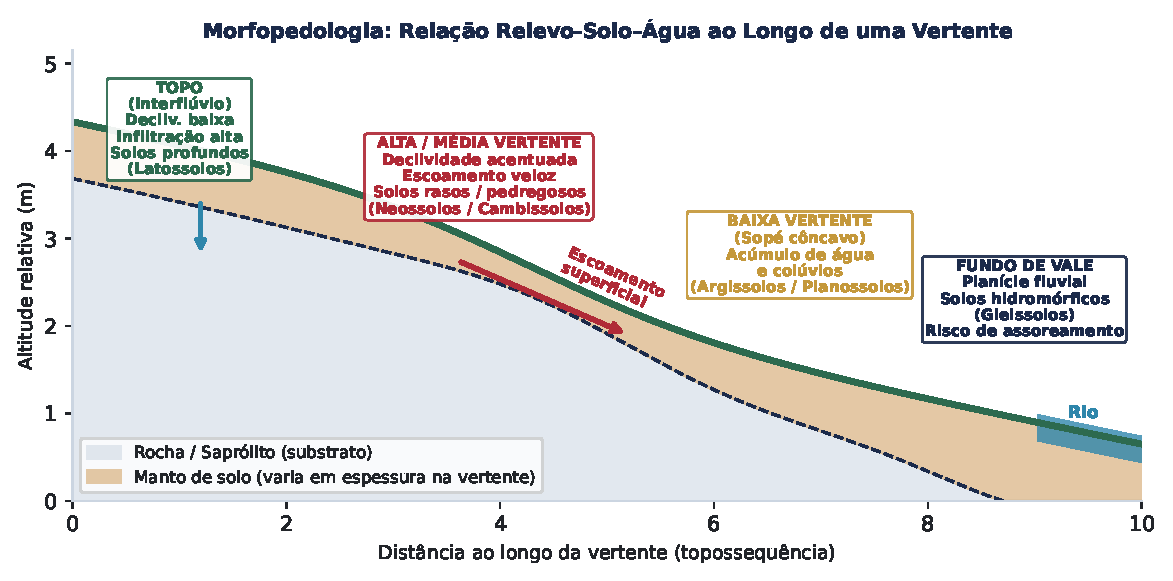
\includegraphics[width=0.94\textwidth]{figures/fig06_morfopedologia_vertente.pdf}
  \caption{Perfil morfopedológico integrado de uma vertente (topossequência), evidenciando a variação da espessura do manto de solo, do balanço infiltração/escoamento e das classes pedológicas do topo ao fundo de vale.}
  \label{fig:morfopedologia_vertente}
\end{figure}

\begin{table}[H]
\centering
\caption{Relação genética entre setores da vertente, dinâmica hídrica, classes de solos e susceptibilidade ambiental.}
\label{tab:topossequencia}
\renewcommand{\arraystretch}{1.20}
\small
\begin{tabularx}{\textwidth}{@{}p{2.3cm} p{2.2cm} p{2.9cm} p{2.7cm} >{\raggedright\arraybackslash}X@{}}
  \toprule
  \rowcolor{uefsNavy}
  \textcolor{white}{\bfseries Setor da Vertente} & \textcolor{white}{\bfseries Forma / Declividade} & \textcolor{white}{\bfseries Dinâmica Hídrica Dominante} & \textcolor{white}{\bfseries Solos Típicos (SiBCS)} & \textcolor{white}{\bfseries Fragilidade / Processo Principal} \\
  \midrule
  Topo (interflúvio) & Plano a suave ($< 8\%$) & Infiltração vertical intensa & Latossolos (profundos) & Baixa erosão natural; sensível à compactação agrícola. \\
  \rowcolor{bgGray}
  Ombro (alta vertente) & Convexo ($8\text{--}20\%$) & Aceleração do escoamento difuso & Latossolos / Argissolos & Erosão laminar e início de sulcos em solo exposto. \\
  Meia encosta & Retilíneo íngreme ($> 20\%$) & Escoamento veloz e remoção ativa & Neossolos Litólicos e Cambissolos & Alta fragilidade: ravinas e movimentos de massa. \\
  \rowcolor{bgGray}
  Sopé (baixa vertente) & Côncavo ($3\text{--}12\%$) & Convergência de fluxos e coluvionamento & Argissolos e Planossolos & Erosão em ravinas/voçorocas por fluxo subsuperficial. \\
  Fundo de vale & Plano ($< 3\%$) & Saturação hídrica e inundação & Gleissolos e Neossolos Flúvicos & Assoreamento do canal e inundações sazonais. \\
  \bottomrule
\end{tabularx}
\end{table}

\section{Declividade da Vertente: Cálculo e Classificação (EMBRAPA e Ross)}

A \textbf{declividade} é o principal parâmetro quantitativo que expressa a energia gravitacional atuante sobre uma encosta. Quanto maior a declividade, maior é a componente tangencial da gravidade que acelera o escoamento superficial e solicita o solo ao cisalhamento (deslizamento). Na Geografia e na Engenharia Ambiental, a declividade é expressa de duas maneiras complementares: em \textbf{porcentagem ($S\%$)} e em \textbf{graus ($\theta$)}.

\begin{boxFormula}[Declividade de Vertentes em Porcentagem ($S\%$) e em Graus ($\theta$)]
\textbf{Origem e finalidade:} derivada da trigonometria do triângulo retângulo formado pela projeção horizontal e pelo desnível vertical do terreno, a declividade quantifica o grau de inclinação de uma rampa para fins de mapeamento pedológico (EMBRAPA), análise de fragilidade ambiental (Ross, 1994), planejamento urbano e aplicação do Código Florestal (encostas com $\theta > 45^\circ$, ou $S > 100\%$, são APPs).

\textbf{Equações fundamentais:}
\[
  S(\%) = \frac{\Delta h}{d_h} \times 100 \qquad\text{e}\qquad \theta = \arctan\!\left(\frac{\Delta h}{d_h}\right)
\]
\textbf{Relações auxiliares indispensáveis em Geografia:}
\begin{itemize}[leftmargin=1.5em, itemsep=1.5pt]
  \item \textbf{A partir de carta topográfica (escala $1:E$):} se a distância medida no mapa entre duas curvas de nível é $d_{\text{mapa}}$ (em metros ou convertida de cm para m), então $d_h = d_{\text{mapa}} \times E$.
  \item \textbf{A partir de trena no terreno (distância inclinada $d_{\text{inc}}$):} pelo Teorema de Pitágoras, obtém-se primeiro a distância horizontal:
  \[
    d_h = \sqrt{d_{\text{inc}}^2 - \Delta h^2}.
  \]
  \item \textbf{Conversão direta entre graus e porcentagem:} $S(\%) = 100 \cdot \tan\theta$ e $\theta = \arctan(S / 100)$.
\end{itemize}

\textbf{Variáveis e unidades:} $\Delta h$ e $d_h$ devem estar obrigatoriamente na \textbf{mesma unidade de comprimento} (ambos em metros, por exemplo).

\textbf{Exemplo numérico completo:} uma encosta desce da cota $316\text{ m}$ para a cota $280\text{ m}$ ao longo de uma distância horizontal de $d_h = 200\text{ m}$.
\begin{align*}
  \Delta h &= 316 - 280 = 36\text{ m} \\
  S(\%) &= \frac{36}{200} \times 100 = 0,18 \times 100 = 18,0\% \\
  \theta &= \arctan(0,18) \approx 10,20^\circ.
\end{align*}
\textbf{Interpretação:} a cada $100\text{ m}$ percorridos na horizontal, o terreno sobe ou desce $18\text{ m}$. Pelas classes da Tabela~\ref{tab:classes_declividade}, o relevo é \textbf{Ondulado} (EMBRAPA) e apresenta \textbf{Fragilidade Média — Classe 3} (Ross, 1994).
\end{boxFormula}

Note um marco conceitual que elimina erros em provas: \textbf{uma declividade de $45^\circ$ corresponde exatamente a $100\%$}, pois $\tan(45^\circ) = 1$, o que significa que $\Delta h = d_h$ (o terreno sobe $1\text{ m}$ a cada $1\text{ m}$ na horizontal). Consequentemente, rampas mais íngremes que $45^\circ$ possuem declividades \textbf{superiores a $100\%$} (por exemplo, $60^\circ$ equivale a $\tan(60^\circ) \times 100 \approx 173,2\%$).

\begin{table}[H]
\centering
\caption{Classes de declividade segundo a EMBRAPA (relevo pedológico) e segundo Ross (1994) (fragilidade do relevo), com correspondência aproximada em graus e implicações ambientais.}
\label{tab:classes_declividade}
\renewcommand{\arraystretch}{1.18}
\small
\begin{tabularx}{\textwidth}{@{}p{2.3cm} p{2.1cm} p{2.6cm} p{2.5cm} >{\raggedright\arraybackslash}X@{}}
  \toprule
  \rowcolor{uefsNavy}
  \textcolor{white}{\bfseries EMBRAPA ($S\%$)} & \textcolor{white}{\bfseries Ângulo ($\theta^\circ$)} & \textcolor{white}{\bfseries Classe EMBRAPA} & \textcolor{white}{\bfseries Classe Ross (1994)} & \textcolor{white}{\bfseries Implicações de Uso e Processos Dominantes} \\
  \midrule
  $0\text{ a } 3\%$ & $0^\circ\text{ a } 1,7^\circ$ & Plano & \multirow{2}{2.5cm}{$< 6\%$ ($\approx 3,4^\circ$): \newline \textbf{1 — Muito Fraca}} & Escoamento lento; predomínio da infiltração; risco de encharcamento em várzeas. \\
  \rowcolor{bgGray}
  $3\text{ a } 8\%$ & $1,7^\circ\text{ a } 4,6^\circ$ & Suave ondulado & & Baixo potencial erosivo; apto à mecanização agrícola com práticas simples. \\
  $8\text{ a } 20\%$ & $4,6^\circ\text{ a } 11,3^\circ$ & Ondulado & $6\text{ a } 12\%$: \textbf{2 — Fraca} \newline $12\text{ a } 20\%$: \textbf{3 — Média} & Escoamento superficial ganha energia; exige plantio em nível, terraceamento e conservação. \\
  \rowcolor{bgGray}
  $20\text{ a } 45\%$ & $11,3^\circ\text{ a } 24,2^\circ$ & Forte ondulado & $20\text{ a } 30\%$: \textbf{4 — Forte} \newline $> 30\%$: \textbf{5 — M. Forte} & Restrito à urbanização e culturas anuais; alta suscetibilidade a erosão linear e deslizamentos. \\
  $45\text{ a } 75\%$ & $24,2^\circ\text{ a } 36,9^\circ$ & Montanhoso & $> 30\%$: \textbf{5 — M. Forte} & Uso restrito à preservação florestal e conservação; movimentos de massa frequentes se desmatado. \\
  \rowcolor{bgGray}
  $> 75\%$ & $> 36,9^\circ$ & Escarpado & $> 30\%$: \textbf{5 — M. Forte} & Escarpas abruptas; acima de $45^\circ$ ($100\%$) constitui APP legal (Lei 12.651/2012). \\
  \bottomrule
\end{tabularx}
\end{table}

\section{Cobertura Vegetal, Erosão em Vertentes e Movimentos de Massa}

\subsection{Papel da Cobertura Vegetal no Balanço Infiltração vs. Escoamento}
A cobertura vegetal constitui a primeira linha de defesa da vertente contra a degradação. Sua atuação ocorre em três níveis integrados:
\begin{enumerate}[leftmargin=1.6em, itemsep=2pt]
  \item \textbf{Dossel aéreo (copas e estratos arbustivos):} intercepta parte da chuva (retornando-a à atmosfera por evaporação) e quebra a energia cinética das gotas antes que atinjam o solo, impedindo o efeito \textbf{splash} (salpicamento) que desagrega torrões e cria crostas de selamento superficial.
  \item \textbf{Serapilheira (folhedo sobre o solo):} funciona como manta protetora de alta rugosidade hidráulica, reduzindo a velocidade do escoamento superficial e ampliando o tempo disponível para a água penetrar no solo.
  \item \textbf{Sistema radicular e atividade biológica:} raízes e fauna edáfica formam canais contínuos (\textbf{macroporosidade}) que elevam drasticamente a taxa de infiltração; simultaneamente, a evapotranspiração retira excesso de água do perfil (reduzindo a poropressão positiva) e as raízes acrescentam resistência mecânica ao cisalhamento (coesão radicular, tema aprofundado no Cap. 13).
\end{enumerate}

Quando essa proteção é removida, o escoamento superficial concentrado evolui progressivamente de erosão laminar para sulcos, ravinas e voçorocas (detalhados no Cap. 12), exportando grandes volumes de solo para o sopé e para os canais fluviais, onde geram \textbf{assoreamento}, caracterizado pela redução da profundidade da calha, pela perda de capacidade de armazenamento de açudes e pela ampliação das manchas de inundação.

\subsection{Movimentos de Massa em Encostas}
Enquanto a erosão hídrica transporta partículas de solo gradualmente pela ação da água corrente, os \textbf{movimentos de massa} (ou movimentos gravitacionais de massa) consistem no deslocamento coletivo de volumes expressivos de solo, saprólito e/ou rocha encosta abaixo, impulsionados diretamente pela força da gravidade quando as tensões cisalhantes superam a resistência interna do material (Guerra, 2018; Varnes, 1978).

Na análise ambiental e na gestão de riscos em encostas, processos frequentes em áreas serranas e em bairros periféricos sobre relevo acidentado na Bahia (como Salvador, cidades do Recôncavo e bordas de serras), distinguem-se cinco tipos principais, sistematizados na Tabela~\ref{tab:movimentos_massa}.

\begin{table}[H]
\centering
\caption{Quadro comparativo dos principais tipos de movimentos de massa em encostas.}
\label{tab:movimentos_massa}
\renewcommand{\arraystretch}{1.20}
\small
\begin{tabularx}{\textwidth}{@{}p{2.5cm} p{2.0cm} p{2.6cm} p{3.1cm} >{\raggedright\arraybackslash}X@{}}
  \toprule
  \rowcolor{uefsNavy}
  \textcolor{white}{\bfseries Tipo de Movimento} & \textcolor{white}{\bfseries Velocidade} & \textcolor{white}{\bfseries Geometria / Mecanismo} & \textcolor{white}{\bfseries Principais Gatilhos} & \textcolor{white}{\bfseries Feições Diagnósticas em Campo} \\
  \midrule
  \textbf{Rastejo (\textit{creep})} & Muito lenta ($\text{mm}$ a $\text{cm}/\text{ano}$) & Deformação plástica contínua sem plano nítido de ruptura & Ciclos de umedecimento/secagem e gravidade contínua & Árvores com troncos encurvados na base, cercas e postes inclinados, trincas lentas em muros. \\
  \rowcolor{bgGray}
  \textbf{Escorregamento rotacional} & Moderada a rápida ($\text{m/h}$ a $\text{m/s}$) & Superfície de ruptura curva (côncava em forma de colher) & Chuvas prolongadas, elevação da poropressão, cortes no pé do talude & Cicatriz em arco no topo, degrau de abatimento, massa tombada para trás e lóbulo no pé. \\
  \textbf{Escorregamento translacional (planar)} & Rápida a muito rápida ($\text{m/s}$) & Superfície de ruptura plana (contato solo–rocha ou fratura) & Chuvas intensas rápidas em solos rasos de encostas íngremes & Cicatriz rasa e alongada expondo rocha/saprólito; material desliza como placa extensa. \\
  \rowcolor{bgGray}
  \textbf{Corrida de lama / detritos} & Muito rápida a extremamente rápida & Fluxo viscoso saturado comportando-se como fluido denso & Chuvas extremas canalizadas em vales íngremes com solo solto & Canais escavados em U, blocos arrastados a longas distâncias e leques espessos no sopé. \\
  \textbf{Queda de blocos} & Extremamente rápida (queda livre) & Desprendimento abrupto de blocos em paredões subverticais & Fraturamento rochoso, alívio de tensão, raízes em fendas, chuvas & Acúmulo de blocos angulosos (depósito de tálus) na base de escarpas e falésias. \\
  \bottomrule
\end{tabularx}
\end{table}

\begin{boxConceito}[Fatores Naturais vs. Antrópicos na Fragilidade de Encostas]
A instabilidade de uma vertente resulta da interação entre \textbf{fatores condicionantes} (declividade elevada, solos rasos sobre rocha impermeável, fraturas inclinadas a favor do talude) e \textbf{fatores deflagradores} (chuvas intensas ou prolongadas). A ocupação humana desordenada agrava criticamente ambos os lados dessa equação ao: (1) executar \textbf{cortes verticais no pé da encosta} (removendo o apoio lateral natural); (2) lançar \textbf{aterros mal compactados e lixo} no topo (aumentando o peso solicitante); (3) infiltrar \textbf{águas servidas e fossas} diretamente no talude (elevando a poropressão mesmo fora do período chuvoso); e (4) suprimir a cobertura vegetal arbórea.
\end{boxConceito}

\etapa{4}{Estudos de Caso e Exemplos Resolvidos Passo a Passo}

\begin{boxExemplo}{8.1}{Declividade e Solos ao Longo de uma Topossequência (Nível Básico)}
\passoEnunciado{Durante um trabalho de campo da disciplina CHF662, os estudantes levantaram três segmentos consecutivos de uma mesma vertente: o \textbf{Topo} (desnível de $6\text{ m}$ em $300\text{ m}$ horizontais), a \textbf{Meia Encosta} (desnível de $54\text{ m}$ em $150\text{ m}$ horizontais) e o \textbf{Sopé} (desnível de $12\text{ m}$ em $200\text{ m}$ horizontais).}
\passoDados{Topo: $\Delta h = 6\text{ m}, d_h = 300\text{ m}$. Meia Encosta: $\Delta h = 54\text{ m}, d_h = 150\text{ m}$. Sopé: $\Delta h = 12\text{ m}, d_h = 200\text{ m}$.}
\passoPedido{Calcular a declividade em porcentagem ($S\%$) e em graus ($\theta$) de cada setor, classificá-los segundo EMBRAPA e Ross (1994) e indicar o solo esperado em cada posição da topossequência.}
\passoMetodo{Aplicação de $S(\%) = (\Delta h / d_h)\times 100$ e $\theta = \arctan(\Delta h / d_h)$, com enquadramento pelas Tabelas~\ref{tab:topossequencia} e~\ref{tab:classes_declividade}.}
\passoContas{%
\begin{enumerate}[leftmargin=1.6em, itemsep=2pt]
  \item \textbf{Topo:}
  \[
    S_1 = \frac{6}{300} \times 100 = 0,02 \times 100 = 2,0\% \qquad;\qquad \theta_1 = \arctan(0,02) \approx 1,15^\circ.
  \]
  \item \textbf{Meia Encosta:}
  \[
    S_2 = \frac{54}{150} \times 100 = 0,36 \times 100 = 36,0\% \qquad;\qquad \theta_2 = \arctan(0,36) \approx 19,80^\circ.
  \]
  \item \textbf{Sopé:}
  \[
    S_3 = \frac{12}{200} \times 100 = 0,06 \times 100 = 6,0\% \qquad;\qquad \theta_3 = \arctan(0,06) \approx 3,43^\circ.
  \]
\end{enumerate}}
\passoResposta{Topo: $2,0\%$ ($1,15^\circ$) — EMBRAPA Plano / Ross Classe 1 (Muito Fraca), com predomínio de \textbf{Latossolos}. Meia Encosta: $36,0\%$ ($19,80^\circ$) — EMBRAPA Forte ondulado / Ross Classe 5 (Muito Forte, $>30\%$), com \textbf{Neossolos Litólicos / Cambissolos}. Sopé: $6,0\%$ ($3,43^\circ$) — EMBRAPA Suave ondulado / Ross Classe 2 (Fraca, $6\text{--}12\%$), com \textbf{Argissolos / Planossolos}.}
\passoVerificacao{O perfil numérico reproduz o comportamento clássico da Figura~\ref{fig:morfopedologia_vertente}: declividade mínima no topo (máxima infiltração e solo profundo), salto abrupto na meia encosta (predomínio erosivo e solo raso) e suavização no sopé (acumulação coluvial).}
\end{boxExemplo}

\begin{boxExemplo}{8.2}{Cálculo de Declividade a partir de Carta Topográfica (Nível Básico–Intermediário)}
\passoEnunciado{Em uma carta topográfica na escala \textbf{1:25.000}, duas curvas de nível de cotas $260\text{ m}$ e $320\text{ m}$ estão separadas, em linha reta perpendicular às curvas, por uma distância medida na régua de $d_{\text{mapa}} = 1,2\text{ cm}$.}
\passoDados{Escala $1:25.000$ ($E = 25.000$); $H_1 = 260\text{ m}$; $H_2 = 320\text{ m}$; $d_{\text{mapa}} = 1,2\text{ cm}$.}
\passoPedido{Determinar a distância horizontal real ($d_h$), o desnível ($\Delta h$), a declividade em porcentagem ($S\%$) e em graus ($\theta$), e sua classe segundo EMBRAPA e Ross.}
\passoMetodo{Conversão da distância cartográfica para distância horizontal real em metros ($d_h = d_{\text{mapa}} \times E$), seguida do cálculo de $S(\%)$ e $\theta$.}
\passoContas{%
\begin{enumerate}[leftmargin=1.6em, itemsep=2pt]
  \item \textbf{Distância horizontal real ($d_h$):}
  \[
    d_h = 1,2\text{ cm} \times 25.000 = 30.000\text{ cm}.
  \]
  Convertendo centímetros para metros (dividindo por $100$):
  \[
    d_h = \frac{30.000}{100} = 300\text{ m}.
  \]
  \item \textbf{Desnível vertical ($\Delta h$):}
  \[
    \Delta h = 320 - 260 = 60\text{ m}.
  \]
  \item \textbf{Declividade em porcentagem e em graus:}
  \[
    S(\%) = \frac{60}{300} \times 100 = 0,20 \times 100 = 20,0\% \qquad;\qquad \theta = \arctan(0,20) \approx 11,31^\circ.
  \]
\end{enumerate}}
\passoResposta{$d_h = 300\text{ m}$, $\Delta h = 60\text{ m}$, $S = 20,0\%$ e $\theta \approx 11,31^\circ$. Classe EMBRAPA: limite superior de Ondulado ($8\text{--}20\%$); Classe Ross: início da Classe 4 — Forte ($20\text{--}30\%$).}
\passoVerificacao{Em escala 1:25.000, cada $1\text{ cm}$ vale $250\text{ m}$; logo $1,2\text{ cm}$ corresponde a $250 + 50 = 300\text{ m}$, confirmando a conversão. Como $60 / 300 = 1/5 = 0,20$, a declividade de $20\%$ e o ângulo de $11,31^\circ$ são exatos e alertam para a necessidade de práticas conservacionistas rigorosas.}
\end{boxExemplo}

\begin{boxExemplo}{8.3}{Correção de Distância Inclinada Medida com Trena em Campo (Nível Intermediário)}
\passoEnunciado{Durante uma vistoria de encosta sem mapa detalhado, um técnico mediu com trena apoiada sobre a superfície do terreno uma rampa de comprimento inclinado $d_{\text{inc}} = 100\text{ m}$. Com auxílio de nível topográfico/altímetro de precisão, verificou-se um desnível vertical de $\Delta h = 28\text{ m}$ entre a base e o topo dessa rampa.}
\passoDados{$d_{\text{inc}} = 100\text{ m}$; $\Delta h = 28\text{ m}$.}
\passoPedido{Calcular a distância horizontal real ($d_h$), a declividade correta ($S\%$ e $\theta$) e mostrar qual seria o erro caso o técnico utilizasse indevidamente $d_{\text{inc}}$ no lugar de $d_h$.}
\passoMetodo{Aplicação do Teorema de Pitágoras ($d_h = \sqrt{d_{\text{inc}}^2 - \Delta h^2}$) antes de calcular $S(\%) = (\Delta h / d_h)\times 100$ e $\theta = \arctan(\Delta h / d_h)$.}
\passoContas{%
\begin{enumerate}[leftmargin=1.6em, itemsep=2pt]
  \item \textbf{Cálculo da distância horizontal ($d_h$):}
  \[
    d_h = \sqrt{100^2 - 28^2} = \sqrt{10.000 - 784} = \sqrt{9.216} = 96,0\text{ m}.
  \]
  \item \textbf{Declividade correta em porcentagem e graus:}
  \[
    S(\%) = \frac{28}{96} \times 100 \approx 0,2917 \times 100 = 29,17\% \qquad;\qquad \theta = \arctan\!\left(\frac{28}{96}\right) \approx 16,26^\circ.
  \]
  \item \textbf{Comparação com o erro de usar $d_{\text{inc}}$ diretamente:} se o técnico dividisse $28 / 100$, obteria $28,00\%$ (subestimando a declividade em $1,17$ ponto percentual, pois $28/100 = \sin\theta$ e não $\tan\theta$).
\end{enumerate}}
\passoResposta{$d_h = 96,0\text{ m}$; declividade correta $S = 29,17\%$ e $\theta \approx 16,26^\circ$ (EMBRAPA: Forte ondulado; Ross: Classe 4 — Forte, quase no limite da Classe 5).}
\passoVerificacao{Como a hipotenusa ($d_{\text{inc}} = 100\text{ m}$) é sempre maior que o cateto horizontal ($d_h = 96\text{ m}$), usar a distância medida pela trena no denominador sempre subestima a declividade real, erro que se torna muito grave em encostas acima de $30\%$.}
\end{boxExemplo}

\begin{boxExemplo}{8.4}{Efeito da Cobertura Vegetal no Balanço Infiltração vs. Escoamento (Nível Intermediário)}
\passoEnunciado{Duas parcelas experimentais adjacentes em uma mesma meia encosta ($S = 18\%$) receberam uma chuva de $80\text{ mm}$: a \textbf{Parcela 1} possui cobertura de Caatinga arbóreo-arbustiva conservada com serapilheira (infiltração/retenção de $85\%$ e escoamento superficial de $15\%$); a \textbf{Parcela 2} encontra-se com solo exposto após queimada e pisoteio bovino (infiltração de $25\%$ e escoamento superficial de $75\%$).}
\passoDados{Chuva total $P = 80\text{ mm}$. Parcela 1: $85\%$ infiltração, $15\%$ escoamento. Parcela 2: $25\%$ infiltração, $75\%$ escoamento.}
\passoPedido{Calcular as lâminas infiltradas e escoadas (em $\text{mm}$ e em litros por $\text{m}^2$) em cada parcela, a razão entre os escoamentos e os reflexos morfopedológicos esperados.}
\passoMetodo{Cálculo proporcional das lâminas ($L_{\text{inf}}$ e $L_{\text{esc}}$) usando a equivalência $1\text{ mm} = 1\text{ L/m}^2$.}
\passoContas{%
\begin{enumerate}[leftmargin=1.6em, itemsep=2pt]
  \item \textbf{Parcela 1 (vegetação conservada):}
  \begin{align*}
    L_{\text{inf},1} &= 0,85 \times 80\text{ mm} = 68,0\text{ mm} \;\; (68\text{ L/m}^2) \\
    L_{\text{esc},1} &= 0,15 \times 80\text{ mm} = 12,0\text{ mm} \;\; (12\text{ L/m}^2).
  \end{align*}
  \item \textbf{Parcela 2 (solo exposto):}
  \begin{align*}
    L_{\text{inf},2} &= 0,25 \times 80\text{ mm} = 20,0\text{ mm} \;\; (20\text{ L/m}^2) \\
    L_{\text{esc},2} &= 0,75 \times 80\text{ mm} = 60,0\text{ mm} \;\; (60\text{ L/m}^2).
  \end{align*}
  \item \textbf{Comparação do escoamento superficial:}
  \[
    \frac{L_{\text{esc},2}}{L_{\text{esc},1}} = \frac{60,0}{12,0} = 5,0\text{ vezes}.
  \]
\end{enumerate}}
\passoResposta{Na parcela conservada infiltram $68\text{ L/m}^2$ e escoam $12\text{ L/m}^2$; no solo exposto infiltram apenas $20\text{ L/m}^2$ e escoam $60\text{ L/m}^2$, um volume superficial $5$ vezes maior.}
\passoVerificacao{Observe a soma em ambas as parcelas ($68 + 12 = 80\text{ mm}$; $20 + 60 = 80\text{ mm}$). Sobre uma vertente de $18\%$, multiplicar o escoamento por cinco sem a rugosidade da serapilheira desencadeia rapidamente erosão laminar, sulcos e assoreamento do sopé, além de reduzir em $70,6\%$ a água disponível para recarga e sobrevivência da vegetação na estação seca.}
\end{boxExemplo}

\begin{boxExemplo}{8.5}{Instabilização de Encosta Urbana por Corte de Talude (Nível Avançado)}
\passoEnunciado{Uma encosta natural com solo argilo-arenoso espesso apresenta desnível $\Delta h = 27\text{ m}$ distribuído ao longo de uma distância horizontal $d_{h1} = 150\text{ m}$. Para implantar um conjunto de residências sem projeto geotécnico, executou-se um corte no sopé da vertente, concentrando o mesmo desnível de $27\text{ m}$ em uma distância horizontal reduzida para $d_{h2} = 45\text{ m}$, acompanhado de lançamento de águas servidas a montante.}
\passoDados{$\Delta h = 27\text{ m}$; cenário natural $d_{h1} = 150\text{ m}$; cenário após corte $d_{h2} = 45\text{ m}$.}
\passoPedido{Calcular a declividade ($S\%$ e $\theta$) antes e depois da intervenção, verificar se ultrapassa o limite de APP de $45^\circ$ ($100\%$), identificar o tipo de movimento de massa mais provável e justificar os mecanismos envolvidos.}
\passoMetodo{Cálculo comparativo de $S(\%)$ e $\theta$ e diagnóstico geotécnico-morfopedológico baseado na Tabela~\ref{tab:movimentos_massa}.}
\passoContas{%
\begin{enumerate}[leftmargin=1.6em, itemsep=2pt]
  \item \textbf{Encosta natural ($d_{h1} = 150\text{ m}$):}
  \[
    S_1 = \frac{27}{150} \times 100 = 18,0\% \qquad;\qquad \theta_1 = \arctan(0,18) \approx 10,20^\circ.
  \]
  \item \textbf{Talude após corte ($d_{h2} = 45\text{ m}$):}
  \[
    S_2 = \frac{27}{45} \times 100 = 60,0\% \qquad;\qquad \theta_2 = \arctan(0,60) \approx 30,96^\circ.
  \]
  \item \textbf{Verificação do limite legal de $45^\circ$ ($100\%$):} como $30,96^\circ < 45^\circ$ ($60\% < 100\%$), o talude não atingiu o patamar de APP de encosta ($>45^\circ$), mas saltou da Classe 3 de Ross (Média) para a \textbf{Classe 5 (Muito Forte, $>30\%$)} e da classe Ondulado para \textbf{Montanhoso (EMBRAPA)}.
\end{enumerate}}
\passoResposta{A declividade mais que triplicou, passando de $18,0\%$ ($10,20^\circ$) para $60,0\%$ ($30,96^\circ$). Em solo argilo-arenoso espesso sujeito a corte no pé e saturação por águas servidas, o movimento de massa mais provável é o \textbf{escorregamento rotacional}.}
\passoVerificacao{O resultado demonstra um ponto crucial de Análise Ambiental: uma encosta não precisa atingir $45^\circ$ ($100\%$) para apresentar risco crítico! O corte retira o contraforte natural na base do maciço de solo, enquanto as águas servidas elevam a poropressão e reduzem o atrito interno, criando condições clássicas para ruptura curva (rotacional) durante eventos de chuva prolongada.}
\end{boxExemplo}

\etapa{5}{Erros Mais Comuns em Provas e Diagnósticos}

\begin{boxErro}[Erro 1 — Achar que $100\%$ de declividade equivale a um paredão vertical de $90^\circ$]
\textbf{Equívoco frequente:} associar intuitivamente $100\%$ ao ângulo reto ($90^\circ$) e concluir que $45^\circ$ valeria $50\%$.

\textbf{Correção técnica:} a declividade em porcentagem é $100 \times \tan\theta$. Como $\tan(45^\circ) = 1$, uma encosta de \textbf{$45^\circ$ tem exatamente $100\%$ de declividade} ($\Delta h = d_h$). Já uma parede vertical ($90^\circ$) possui $d_h = 0$, tendendo a declividade ao infinito.
\end{boxErro}

\begin{boxErro}[Erro 2 — Usar a distância inclinada da trena no denominador de $S(\%)$]
\textbf{Equívoco frequente:} medir $50\text{ m}$ inclinados no terreno com trena e dividir $\Delta h$ diretamente por $50\text{ m}$.

\textbf{Correção técnica:} a definição matemática de declividade usa a \textbf{distância horizontal ($d_h$)} no denominador ($\Delta h / d_h = \tan\theta$). Quando se dispõe apenas da distância inclinada ($d_{\text{inc}}$), deve-se calcular $d_h = \sqrt{d_{\text{inc}}^2 - \Delta h^2}$ antes de aplicar a fórmula.
\end{boxErro}

\begin{boxErro}[Erro 3 — Confundir escorregamento rotacional com translacional]
\textbf{Equívoco frequente:} chamar qualquer deslizamento de terra genericamente de "desmoronamento" ou trocar os condicionantes de cada tipo.

\textbf{Correção técnica:} o \textbf{escorregamento rotacional} ocorre tipicamente em solos espessos e homogêneos, formando superfície de ruptura curva (em colher); o \textbf{escorregamento translacional (planar)} ocorre em solos rasos sobre substrato rochoso ou planos de fraqueza, deslizando como uma placa paralela à superfície da encosta.
\end{boxErro}

\begin{boxErro}[Erro 4 — Analisar solo e relevo de forma desarticulada no diagnóstico]
\textbf{Equívoco frequente:} descrever o solo do topo da vertente (ex.: Latossolo profundo) e generalizar suas propriedades de alta permeabilidade para toda a encosta, incluindo a meia vertente íngreme e o fundo de vale.

\textbf{Correção técnica:} pela abordagem morfopedológica, a variação da declividade e da curvatura altera profundamente a pedogênese ao longo da topossequência. Cada compartimento (topo, ombro, meia encosta, sopé e várzea) exige diagnóstico e manejo específicos.
\end{boxErro}

\etapa{6}{Exercícios de Fixação}

\subsection*{Nível Básico (Exercícios 1 a 5)}

\begin{enumerate}[leftmargin=1.8em, itemsep=4pt]
  \item Explique o que é uma \textbf{topossequência} na abordagem morfopedológica e descreva por que os solos do topo plano tendem a ser mais profundos do que os solos da meia encosta íngreme.
  \espacoResolucao[2.0cm]

  \item Uma vertente apresenta desnível vertical $\Delta h = 15\text{ m}$ em uma distância horizontal $d_h = 250\text{ m}$. Calcule sua declividade em porcentagem ($S\%$) e em graus ($\theta$) e classifique-a segundo EMBRAPA e Ross (1994).
  \espacoResolucao[1.8cm]

  \item Determine $S(\%)$ e $\theta$ para uma encosta com $\Delta h = 45\text{ m}$ e $d_h = 150\text{ m}$, indicando sua classe na EMBRAPA e em Ross (1994).
  \espacoResolucao[1.8cm]

  \item Demonstre matematicamente por que uma encosta com $\Delta h = 80\text{ m}$ e $d_h = 80\text{ m}$ corresponde ao limite legal de APP de encosta previsto no Código Florestal ($45^\circ$).
  \espacoResolucao[1.8cm]

  \item Em uma carta topográfica na escala \textbf{1:50.000}, duas curvas de nível separadas por um desnível $\Delta h = 40\text{ m}$ distam $0,8\text{ cm}$ no mapa. Calcule a distância horizontal real ($d_h$) e a declividade ($S\%$ e $\theta$).
  \espacoResolucao[2.0cm]
\end{enumerate}

\subsection*{Nível Intermediário (Exercícios 6 a 10)}

\begin{enumerate}[leftmargin=1.8em, itemsep=4pt, resume]
  \item Em campo, mediu-se com trena sobre a rampa uma distância inclinada $d_{\text{inc}} = 50\text{ m}$ correspondente a um desnível $\Delta h = 14\text{ m}$. Calcule a distância horizontal real ($d_h$) e a declividade correta em porcentagem e em graus.
  \espacoResolucao[2.2cm]

  \item Uma vertente foi dividida em três compartimentos para zoneamento agrícola:
  \begin{itemize}[leftmargin=1.4em, itemsep=1pt]
    \item \textbf{Setor A (topo):} $\Delta h = 10\text{ m}$, $d_h = 400\text{ m}$.
    \item \textbf{Setor B (meia encosta):} $\Delta h = 64\text{ m}$, $d_h = 160\text{ m}$.
    \item \textbf{Setor C (sopé):} $\Delta h = 20\text{ m}$, $d_h = 250\text{ m}$.
  \end{itemize}
  Calcule $S(\%)$ e $\theta$ de cada setor, classifique-os segundo EMBRAPA e Ross e indique o uso mais adequado para cada compartimento.
  \espacoResolucao[2.5cm]

  \item Explique como a remoção da cobertura vegetal altera simultaneamente o efeito \textit{splash}, a macroporosidade superficial e o risco de assoreamento no fundo de vale.
  \espacoResolucao[2.0cm]

  \item Diferencie \textbf{rastejo}, \textbf{escorregamento translacional} e \textbf{corrida de detritos} quanto à velocidade do deslocamento e às feições visíveis em campo.
  \espacoResolucao[2.0cm]

  \item Por que a infiltração de águas servidas (esgoto doméstico sem coleta) em encostas ocupadas pode deflagrar movimentos de massa mesmo após chuvas moderadas? Utilize o conceito de \textbf{poropressão} na sua explicação.
  \espacoResolucao[2.0cm]
\end{enumerate}

\subsection*{Questões Objetivas (Exercícios 11 a 15)}

\begin{enumerate}[leftmargin=1.8em, itemsep=5pt, resume]
  \item Ao longo de uma topossequência típica sobre relevo dissecado, espera-se encontrar, respectivamente, no topo plano, na meia encosta íngreme e no fundo de vale hidromórfico:
  \begin{alternativas}
    \item Gleissolos, Latossolos e Neossolos Litólicos.
    \item Latossolos, Neossolos Litólicos/Cambissolos e Gleissolos.
    \item Neossolos Litólicos, Gleissolos e Latossolos.
    \item Planossolos, Latossolos e Neossolos Litólicos.
    \item Cambissolos rasos, Latossolos muito profundos e Argissolos de topo.
  \end{alternativas}

  \item Em uma carta na escala 1:25.000, a distância medida entre a curva de nível de $210\text{ m}$ e a curva de $260\text{ m}$ é de $0,8\text{ cm}$. A declividade desse trecho em porcentagem e sua classe segundo a EMBRAPA são:
  \begin{alternativas}
    \item $12,5\%$ — Ondulado.
    \item $20,0\%$ — Ondulado.
    \item $25,0\%$ — Forte ondulado.
    \item $40,0\%$ — Forte ondulado.
    \item $50,0\%$ — Montanhoso.
  \end{alternativas}

  \item Em uma vistoria técnica de encosta urbana, observaram-se árvores com troncos encurvados na base, postes ligeiramente inclinados para jusante e pequenas trincas progressivas em muros ao longo de anos, sem cicatriz abrupta de ruptura. Esse conjunto de feições é diagnóstico de:
  \begin{alternativas}
    \item Queda de blocos.
    \item Corrida de detritos.
    \item Escorregamento translacional catastrófico.
    \item Rastejo (\textit{creep}).
    \item Erosão por \textit{splash}.
  \end{alternativas}

  \item Assinale a alternativa correta sobre a relação entre declividade em graus e em porcentagem:
  \begin{alternativas}
    \item $45^\circ$ equivale a $50\%$, e $90^\circ$ equivale a $100\%$.
    \item $45^\circ$ equivale a $100\%$, e encostas mais íngremes que $45^\circ$ possuem declividades maiores que $100\%$.
    \item Nenhuma vertente natural pode ultrapassar $100\%$ de declividade.
    \item A declividade em porcentagem é obtida multiplicando o valor em graus por $2$.
    \item Quando $\Delta h = 0$, o ângulo é $45^\circ$.
  \end{alternativas}

  \item Sobre os escorregamentos rotacionais e translacionais, assinale a afirmação correta:
  \begin{alternativas}
    \item O escorregamento rotacional apresenta superfície de ruptura curva e ocorre preferencialmente em mantos de solo espessos e homogêneos.
    \item O escorregamento translacional ocorre apenas em terrenos perfeitamente planos ($< 3\%$).
    \item Cortes verticais no pé de taludes estabilizam a encosta por aliviar o peso do solo.
    \item A cobertura vegetal arbórea aumenta a poropressão positiva ao impedir a evapotranspiração.
    \item O assoreamento do fundo de vale não possui relação com os processos erosivos das vertentes.
  \end{alternativas}
\end{enumerate}

\etapa{7}{Questões de Provas, ENADE e Concursos Ambientais}

\begin{enumerate}[leftmargin=1.8em, itemsep=5pt, start=16]
  \item \textbf{(Questão autoral — estilo ENADE / Geografia)} A abordagem morfopedológica (Casseti, 2007; Ross, 2006; Guerra, 2018) supera a leitura fragmentada do meio físico ao adotar como unidade de análise a integração relevo–solo–água. Nessa perspectiva, a ocorrência de solos rasos e pedregosos (Neossolos Litólicos) na meia encosta retilínea e de solos profundos e bem drenados (Latossolos) no interflúvio aplainado explica-se fundamentalmente porque:
  \begin{alternativas}
    \item A precipitação atmosférica incide apenas nos topos planos, não alcançando as encostas inclinadas.
    \item No topo aplainado predomina a infiltração vertical e o intemperismo profundo (pedogênese), enquanto na meia encosta íngreme a energia do escoamento remove continuamente o manto de alteração (morfogênese).
    \item Os Latossolos são transportados inteiros pela gravidade dos fundos de vale para os topos.
    \item As rochas do fundo de vale são sempre mais resistentes ao intemperismo do que as do topo.
    \item A declividade não influencia o balanço entre infiltração e escoamento superficial.
  \end{alternativas}

  \item \textbf{(Questão autoral — estilo Concurso Perito / Analista Ambiental)} Durante um levantamento de fragilidade de encosta para licenciamento de um empreendimento linear, constatou-se que determinado trecho possui desnível vertical $\Delta h = 90\text{ m}$ em uma distância horizontal $d_h = 250\text{ m}$, com solo raso sobre substrato rochoso pouco permeável. Assinale a alternativa que apresenta corretamente a declividade ($S\%$ e $\theta$), a classificação de Ross (1994) e o movimento de massa de maior risco em caso de supressão vegetal e chuvas intensas:
  \begin{alternativas}
    \item $S = 36,0\%$; $\theta \approx 19,80^\circ$; Classe 5 de Ross (Muito Forte); escorregamento translacional (planar).
    \item $S = 27,8\%$; $\theta \approx 15,50^\circ$; Classe 4 de Ross (Forte); queda livre de blocos em paredão vertical.
    \item $S = 36,0\%$; $\theta \approx 19,80^\circ$; Classe 3 de Ross (Média); rastejo imperceptível sem risco imediato.
    \item $S = 18,0\%$; $\theta \approx 10,20^\circ$; Classe 2 de Ross (Fraca); erosão eólica dominante.
    \item $S = 90,0\%$; $\theta \approx 42,00^\circ$; Classe 5 de Ross (Muito Forte); subsidência cárstica.
  \end{alternativas}

  \item \textbf{(Questão autoral — estilo Concurso Defesa Civil / Geologia e Geografia Ambiental)} Em áreas urbanas brasileiras construídas sobre encostas de declividade acentuada, a prevenção de desastres por movimentos de massa requer intervenções integradas. Entre as medidas abaixo, aquela que \textbf{REDUZ efetivamente} a instabilidade da encosta é:
  \begin{alternativas}
    \item Executar cortes subverticais na base da encosta para ampliar lotes residenciais.
    \item Substituir a drenagem superficial por fossas negras infiltrando água diretamente no talude.
    \item Implantar sistema eficiente de drenagem pluvial e coleta de esgoto, evitar cortes/aterros sem contenção e manter ou recompor cobertura vegetal adaptada com técnicas de bioengenharia.
    \item Depositar entulho e solo solto sobre o ombro convexo da vertente para nivelar o terreno.
    \item Remover toda a vegetação de raízes profundas e expor o solo mineral ao sol para acelerar o ressecamento.
  \end{alternativas}
\end{enumerate}

\begin{boxDica}[Articulação Direta com o Capítulo 9 e com o Diagnóstico Final]
Os cinco patamares de declividade de Ross ($<6\%$, $6\text{--}12\%$, $12\text{--}20\%$, $20\text{--}30\%$ e $>30\%$) e o reconhecimento dos tipos de solo da topossequência aprendidos neste capítulo são exatamente os dois primeiros pilares da \textbf{Análise Empírica da Fragilidade Ambiental de Ross (1994)}, que você aplicará integralmente no Capítulo 9!
\end{boxDica}

\clearpage
\etapa{8}{Gabarito Comentado — Exercícios 1 a 18}

\begin{boxGabarito}[Resoluções e Justificativas — Capítulo 8]
\begin{enumerate}[leftmargin=1.8em, itemsep=3.5pt]
  \item \textbf{Topossequência:} é a sucessão ordenada de solos que varia do topo ao fundo de vale em uma mesma vertente. No topo plano, a baixa declividade favorece a infiltração vertical e a permanência do manto de intemperismo (gerando solos profundos como Latossolos); na meia encosta íngreme, a alta velocidade do escoamento remove continuamente partículas superficiais, mantendo os solos rasos e jovens (Neossolos Litólicos/Cambissolos).

  \item \textbf{Cálculo:} $S = (15 / 250) \times 100 = 0,06 \times 100 = \mathbf{6,0\%}$; $\theta = \arctan(0,06) \approx \mathbf{3,43^\circ}$. EMBRAPA: Suave ondulado ($3\text{--}8\%$); Ross: Classe 2 — Fraca ($6\text{--}12\%$).

  \item \textbf{Cálculo:} $S = (45 / 150) \times 100 = 0,30 \times 100 = \mathbf{30,0\%}$; $\theta = \arctan(0,30) \approx \mathbf{16,70^\circ}$. EMBRAPA: Forte ondulado ($20\text{--}45\%$); Ross: limite superior da Classe 4 — Forte ($20\text{--}30\%$).

  \item \textbf{Demonstração:} $S = (80 / 80) \times 100 = 1,0 \times 100 = \mathbf{100,0\%}$ e $\theta = \arctan(1,0) = \mathbf{45,0^\circ}$. Como a Lei nº 12.651/2012 define como APP as encostas ou partes destas com declividade superior a $45^\circ$ (equivalente a $100\%$ na linha de maior declive), esse valor representa exatamente o limiar legal.

  \item \textbf{Carta 1:50.000:} $d_h = 0,8\text{ cm} \times 50.000 = 40.000\text{ cm} = \mathbf{400\text{ m}}$. Declividade: $S = (40 / 400) \times 100 = \mathbf{10,0\%}$; $\theta = \arctan(0,10) \approx \mathbf{5,71^\circ}$ (EMBRAPA: Ondulado; Ross: Classe 2 — Fraca).

  \item \textbf{Correção de trena:} $d_h = \sqrt{50^2 - 14^2} = \sqrt{2.500 - 196} = \sqrt{2.304} = \mathbf{48,0\text{ m}}$. Declividade correta: $S = (14 / 48) \times 100 \approx \mathbf{29,17\%}$; $\theta = \arctan(14 / 48) \approx \mathbf{16,26^\circ}$.

  \item \textbf{Zoneamento dos três setores:}
  \begin{itemize}[leftmargin=1.4em, itemsep=1pt]
    \item \textbf{Setor A:} $S = (10 / 400)\times 100 = \mathbf{2,5\%}$ ($\theta \approx 1,43^\circ$) — Plano / Ross 1 (Muito Fraca): apto à agricultura mecanizada com manejo conservacionista.
    \item \textbf{Setor B:} $S = (64 / 160)\times 100 = \mathbf{40,0\%}$ ($\theta \approx 21,80^\circ$) — Forte ondulado / Ross 5 (Muito Forte): impróprio para lavouras anuais ou urbanização; recomendado para conservação/preservação florestal.
    \item \textbf{Setor C:} $S = (20 / 250)\times 100 = \mathbf{8,0\%}$ ($\theta \approx 4,57^\circ$) — limite Suave ondulado / Ross 2 (Fraca): uso agrícola ou pastagem manejada com curvas de nível e atenção à drenagem do sopé.
  \end{itemize}

  \item \textbf{Cobertura vegetal e assoreamento:} sem o dossel e a serapilheira, as gotas de chuva impactam diretamente o solo (\textit{splash}), quebram agregados e entopem os macroporos superficiais (selamento). A infiltração cai e o escoamento superficial cresce, removendo sedimentos que descem a vertente e se depositam no fundo de vale, assoreando o canal fluvial.

  \item \textbf{Diferenciação:} \textit{rastejo} é muito lento ($\text{mm--cm/ano}$), evidenciado por troncos encurvados e cercas inclinadas; \textit{escorregamento translacional} é rápido ($\text{m/s}$), formando cicatrizes planas e rasas paralelas à encosta; \textit{corrida de detritos} é muito rápida a extremamente rápida, comportando-se como fluido denso que escava canais e forma espessos leques de lama e blocos no sopé.

  \item \textbf{Águas servidas e poropressão:} o lançamento contínuo de esgoto e águas servidas mantém o solo do talude saturado ou próximo da saturação, elevando a \textbf{poropressão ($u$)}. Essa pressão da água nos poros empurra os grãos uns para longe dos outros, reduzindo a tensão efetiva e o atrito interno; assim, mesmo uma chuva moderada já é suficiente para romper o equilíbrio mecânico da encosta.

  \item \textbf{Gabarito: (B).} Sequência clássica da topossequência: Latossolos no topo aplainado, Neossolos Litólicos/Cambissolos na meia encosta íngreme e Gleissolos no fundo de vale hidromórfico.

  \item \textbf{Gabarito: (C).} $d_h = 0,8\text{ cm} \times 25.000 = 20.000\text{ cm} = 200\text{ m}$; $\Delta h = 260 - 210 = 50\text{ m}$; $S = (50 / 200)\times 100 = 25,0\%$ (EMBRAPA: Forte ondulado, faixa de $20\text{--}45\%$).

  \item \textbf{Gabarito: (D).} Deformação lenta e contínua com encurvamento da base de árvores e inclinação de postes/muros caracteriza classicamente o rastejo (\textit{creep}).

  \item \textbf{Gabarito: (B).} Como $S(\%) = 100\cdot\tan\theta$, tem-se $45^\circ \leftrightarrow 100\%$, e para $\theta > 45^\circ$ resulta $S > 100\%$.

  \item \textbf{Gabarito: (A).} Superfície de ruptura curva em solos mais espessos define o escorregamento rotacional. As demais invertem princípios geotécnicos e hidrológicos básicos.

  \item \textbf{Gabarito: (B).} A abordagem morfopedológica demonstra que a baixa declividade no topo privilegia a infiltração e a pedogênese (solos profundos), enquanto a elevada declividade da meia encosta intensifica o escoamento e a morfogênese (solos rasos).

  \item \textbf{Gabarito: (A).} $S = (90 / 250)\times 100 = 36,0\%$; $\theta = \arctan(0,36) \approx 19,80^\circ$. Como $36,0\% > 30\%$, enquadra-se na Classe 5 de Ross (Muito Forte). Em solo raso sobre substrato rochoso pouco permeável sob alta declividade, o mecanismo típico de ruptura é o escorregamento translacional (planar) ao longo do contato solo–rocha.

  \item \textbf{Gabarito: (C).} Drenagem adequada controla a poropressão; evitar cortes/aterros preserva a geometria de equilíbrio; e a cobertura vegetal/bioengenharia acrescenta proteção superficial e coesão radicular.
\end{enumerate}
\end{boxGabarito}

\begin{boxResumo}
\begin{itemize}[leftmargin=1.4em, itemsep=2.5pt]
  \item \textbf{Morfopedologia:} integra formas de relevo, solos e dinâmica hídrica em \textbf{topossequências} (topo com Latossolos profundos $\to$ meia encosta com Neossolos/Cambissolos rasos $\to$ sopé coluvial com Argissolos/Planossolos $\to$ fundo de vale com Gleissolos).
  \item \textbf{Cálculo de Declividade:}
  \[
    S(\%) = \frac{\Delta h}{d_h} \times 100 \qquad;\qquad \theta = \arctan\!\left(\frac{\Delta h}{d_h}\right) \qquad;\qquad 45^\circ \equiv 100\%
  \]
  Em cartas ($1:E$), $d_h = d_{\text{mapa}} \times E$. Em medições de trena inclinada, $d_h = \sqrt{d_{\text{inc}}^2 - \Delta h^2}$.
  \item \textbf{Classes de Ross (declividade):} $<6\%$ (1), $6\text{--}12\%$ (2), $12\text{--}20\%$ (3), $20\text{--}30\%$ (4), $>30\%$ (5).
  \item \textbf{Movimentos de massa:} rastejo (muito lento), escorregamento rotacional (curvo, solo espesso), escorregamento translacional (planar, solo raso), corrida de detritos (fluido rápido) e queda de blocos (paredões rochosos).
\end{itemize}
\end{boxResumo}

\begin{boxTeste}
Responda rapidamente (\V\ ou \F) e confira no gabarito abaixo:
\begin{enumerate}[leftmargin=1.6em, itemsep=2.5pt]
  \item (\quad) Em uma topossequência típica, a meia encosta íngreme apresenta maior taxa de infiltração e solos mais profundos do que o topo plano.
  \item (\quad) Uma encosta com desnível $\Delta h = 30\text{ m}$ e distância horizontal $d_h = 100\text{ m}$ tem declividade de $30\%$ ($\approx 16,7^\circ$).
  \item (\quad) Uma rampa de $45^\circ$ corresponde a uma declividade de $100\%$, pois $\Delta h = d_h$.
  \item (\quad) A infiltração de águas servidas em encostas ocupadas eleva a poropressão e reduz a resistência ao cisalhamento do solo, favorecendo escorregamentos.
\end{enumerate}
\vspace{4pt}
{\footnotesize\textbf{Gabarito do Checkpoint:} 1-\F\ (ocorre o inverso: topo plano tem mais infiltração e solos profundos); 2-\V; 3-\V; 4-\V.}
\end{boxTeste}

% ============================================================================
% MÓDULO 3 — CAPÍTULO 9
% Geossistemas, Ecodinâmica e Análise Empírica da Fragilidade Ambiental (Semana 9)
% ============================================================================

\chapter{Geossistemas, Ecodinâmica e Análise Empírica da Fragilidade Ambiental}
\label{cap:geossistemas_fragilidade}

\noindent\tagEmenta\ \tagPratica

\begin{capObjetivos}
Ao concluir este capítulo (Semana 9 do Plano CHF662), você será capaz de:
\begin{enumerate}[leftmargin=1.6em, itemsep=2pt]
  \item Explicar os princípios da \textbf{Teoria Geral dos Sistemas} (Bertalanffy, 2010) aplicados à paisagem, distinguindo totalidade, fluxos de matéria/energia, homeostase e propriedades emergentes.
  \item Classificar unidades espaciais segundo a \textbf{taxonomia da paisagem} de Bertrand (2004) (zona, domínio, região natural, geossistema, geofácies e geótopo) e aplicar a \textbf{compartimentação geoambiental} (Rodriguez; Silva; Cavalcanti, 2017) ao planejamento.
  \item Diagnosticar o estado dinâmico de unidades territoriais pela \textbf{Ecodinâmica de Tricart (1977)}, avaliando o balanço entre \textbf{morfogênese} e \textbf{pedogênese} em meios estáveis, intergrades e fortemente instáveis.
  \item Aplicar integralmente a \textbf{Análise Empírica da Fragilidade dos Ambientes Naturais e Antropizados} de \textbf{Ross (1994)}, atribuindo as cinco classes hierárquicas (1 a 5) para Relevo/Declividade, Solos, Clima/Pluviosidade e Uso da Terra/Cobertura Vegetal, além de calcular e interpretar os códigos da \textbf{Fragilidade Potencial ($FP$)} e da \textbf{Fragilidade Emergente ($FE$)}.
\end{enumerate}
\end{capObjetivos}

\begin{capRevisao}
Antes de avançar, retome três fundamentos consolidados nos capítulos anteriores:
\begin{itemize}[leftmargin=1.5em, itemsep=2pt]
  \item \textbf{Sistemas ambientais abertos e escalas (Cap. 6):} toda unidade da paisagem troca energia e matéria com o entorno e possui processos próprios em cada escala espacial e temporal; conclusões de detalhe não podem ser extrapoladas linearmente sem ajuste escalar.
  \item \textbf{Bacias hidrográficas e morfopedologia (Caps. 7 e 8):} a bacia fornece o recorte espacial funcional da drenagem, enquanto a vertente revela a interdependência entre declividade ($S\%$), classe de solo (topossequência) e escoamento superficial.
  \item \textbf{Classes de declividade de Ross (Cap. 8):} os cinco patamares de inclinação do terreno ($<6\%$, $6\text{--}12\%$, $12\text{--}20\%$, $20\text{--}30\%$ e $>30\%$) já dominados no Capítulo 8 constituem a primeira variável-chave da matriz de fragilidade ambiental estudada agora.
\end{itemize}
\end{capRevisao}

\etapa{3}{Explicação Teórica: Sistemas, Geossistemas, Ecodinâmica e Fragilidade Ambiental (Ross, 1994)}

\begin{boxSimbolo}[Vocabulário Técnico e Símbolos do Capítulo 9]
A análise integrada da paisagem apoia-se em conceitos sistêmicos e em uma notação específica de fragilidade. Um \textbf{sistema (Bertalanffy, 2010)} corresponde a um conjunto de elementos interdependentes em interação dinâmica, organizado como totalidade funcional capaz de receber entradas (\textit{inputs}), processá-las e emitir saídas (\textit{outputs}). Na escala geográfica, o \textbf{geossistema (Bertrand, 2004)} designa uma unidade espacial homogênea resultante da combinação dinâmica entre potencial ecológico (clima, relevo, hidrologia), exploração biológica (vegetação, solo, fauna) e ação antrópica, subdividindo-se em \textbf{geofácies}, setor fisionomicamente homogêneo (como uma encosta de Caatinga conservada), e em \textbf{geótopo}, a menor unidade espacial (como uma ravina ou afloramento rochoso).

Para diagnosticar o estado dinâmico dessas unidades, a \textbf{Ecodinâmica (Tricart, 1977)} avalia o balanço entre processos de remoção e erosão (\textbf{morfogênese}) e processos de formação de solo (\textbf{pedogênese}). Operacionalmente, a \textbf{Fragilidade Potencial ($FP$)} expressa a suscetibilidade natural intrínseca do ambiente à degradação e à erosão, determinada pelos fatores físicos ($D_R$: Relevo/Declividade; $D_S$: Solos; $D_C$: Clima/Pluviosidade), independentemente da vegetação atual, ao passo que a \textbf{Fragilidade Emergente ($FE$)} traduz a fragilidade real atual, obtida pelo cruzamento de $FP$ com o grau de proteção conferido pelo Uso da Terra e Cobertura Vegetal ($D_U$). Essa informação é sintetizada no \textbf{Código Numérico de Ross}, uma notação posicional formada pelos dígitos das classes de $1$ a $5$, com três dígitos para $FP$ ($D_R D_S D_C$) e quatro dígitos para $FE$ ($D_R D_S D_C D_U$), acompanhada da respectiva classe síntese ($1$ a $5$).
\end{boxSimbolo}

\section{Teoria Geral dos Sistemas (Bertalanffy, 2010) na Análise Ambiental}

Até meados do século XX, grande parte das ciências naturais operava de modo analítico-reducionista, isolando o solo da rocha, a vegetação do clima e o rio das encostas. Ao formular a \textbf{Teoria Geral dos Sistemas (TGS)}, o biólogo \textbf{Ludwig von Bertalanffy (2010)} demonstrou que sistemas complexos não podem ser compreendidos pela simples soma de suas partes isoladas, pois suas propriedades essenciais emergem justamente das \textbf{relações e interações} entre os componentes.

Na Análise Ambiental, a adoção da TGS traduz-se em quatro princípios operacionais articulados. Pelo princípio da \textbf{totalidade e interdependência}, alterar qualquer componente, como remover a cobertura vegetal de uma encosta, modifica imediatamente a infiltração, o escoamento superficial, a temperatura do solo, a erosão e o regime de sedimentos do rio a jusante. Paisagens e bacias hidrográficas operam como \textbf{sistemas abertos e de fluxos contínuos}, recebendo energia solar e precipitação (\textit{inputs}), transformando esses fluxos internamente e exportando água, sedimentos, calor e nutrientes (\textit{outputs}). Sob condições conservadas, esses sistemas mantêm um \textbf{equilíbrio dinâmico (homeostase)} próximo a um estado estacionário graças a mecanismos de autorregulação (\textit{feedback} negativo), mas quando perturbações antrópicas ultrapassam a capacidade de suporte, instala-se a retroalimentação positiva e a degradação acelera-se. Dessa interação conjunta nasce a \textbf{propriedade emergente}, razão pela qual a \textbf{fragilidade ambiental} pertence à combinação simultânea entre os fatores físicos e o uso humano da terra, e nunca a um elemento isolado.

\section{Geossistema, Taxonomia da Paisagem e Compartimentação Geoambiental}

Inspirado na TGS e na escola russo-soviética (Sochava), o geógrafo francês \textbf{Georges Bertrand (2004)} propôs o conceito de \textbf{geossistema} como unidade fundamental para a Geografia Física integrada. Enquanto o ecossistema privilegia as relações tróficas biológicas sem escala espacial rígida, o \textbf{geossistema constitui uma unidade territorial concreta}, situada em uma escala definida (da ordem de alguns quilômetros quadrados a centenas de quilômetros quadrados), onde interagem três conjuntos de forças. O \textbf{Potencial Ecológico} fornece a base abiótica formada por geologia, geomorfologia, clima e hidrologia; a \textbf{Exploração Biológica} reúne vegetação, solos e fauna que colonizam e protegem essa base; e a \textbf{Ação Antrópica} expressa a organização socioeconômica, o uso da terra e as intervenções técnicas que transformam ou conservam o conjunto.

Para evitar a confusão entre escalas regionais e locais (a falácia de escala vista no Cap. 6), Bertrand (2004) estruturou uma \textbf{taxonomia hierárquica da paisagem} em seis níveis, organizados das unidades superiores (zonais/estruturais) às unidades inferiores (dinâmicas/locais), conforme sintetiza a Tabela~\ref{tab:taxonomia_bertrand}.

\begin{table}[H]
\centering
\caption{Taxonomia hierárquica da paisagem segundo Bertrand (2004) e articulação escalar (Rodriguez; Silva; Cavalcanti, 2017).}
\label{tab:taxonomia_bertrand}
\renewcommand{\arraystretch}{1.18}
\small
\begin{tabularx}{\textwidth}{@{}p{2.3cm} p{2.2cm} p{2.3cm} p{3.1cm} >{\raggedright\arraybackslash}X@{}}
  \toprule
  \rowcolor{uefsNavy}
  \textcolor{white}{\bfseries Unidade} & \textcolor{white}{\bfseries Ordem (Escala G)} & \textcolor{white}{\bfseries Escala Cartográfica} & \textcolor{white}{\bfseries Critério Definidor Principal} & \textcolor{white}{\bfseries Exemplo no Brasil / Semiárido} \\
  \midrule
  \multicolumn{5}{@{}l}{\cellcolor{bgGold}\textbf{\color{uefsNavy}Unidades Superiores (condicionamento climático-estrutural)}} \\
  1. Zona & $G\text{I}$ ($>10^7\text{ km}^2$) & $< 1:10.000.000$ & Grandes faixas climáticas planetárias & Zona Intertropical. \\
  \rowcolor{bgGray}
  2. Domínio & $G\text{II}$ ($10^6\text{ km}^2$) & $1:5.000.000$ & Macroestrutura climática, relevo e bioma & Domínio das Caatingas / Depressões Sertanejas. \\
  3. Região Natural & $G\text{III}\text{--}G\text{IV}$ & $1:1.000.000$ & Compartimento geomorfológico e clima regional & Piemonte da Diamantina / Bacia do Rio Jacuípe. \\
  \midrule
  \multicolumn{5}{@{}l}{\cellcolor{bgTeal}\textbf{\color{uefsNavy}Unidades Inferiores (dinâmica integrada e diagnóstico aplicado)}} \\
  4. Geossistema & $G\text{V}$ ($10^1\text{--}10^2\text{ km}^2$) & $1:50.000$ a $1:100.000$ & Combinação potencial ecológico + exploração biológica + antrópica & Geossistema da Serra de São José (Feira de Santana/BA) ou Sub-bacia do Vaza-Barris. \\
  \rowcolor{bgGray}
  5. Geofácies & $G\text{VI}$ ($10^{-1}\text{--}10^0\text{ km}^2$) & $1:10.000$ a $1:25.000$ & Fisionomia homogênea de relevo, solo e cobertura vegetal & Meia encosta com Caatinga arbustiva raleada sobre Neossolo Litólico. \\
  6. Geótopo & $G\text{VII}$ ($<10^{-2}\text{ km}^2$) & $> 1:5.000$ & Microunidade de detalhe extremo e microclima próprio & Parede de voçoroca ativa, lajedo ou talude rodoviário. \\
  \bottomrule
\end{tabularx}
\end{table}

Na prática da Análise Ambiental no Brasil, \textbf{Rodriguez, Silva e Cavalcanti (2017)} avançam da taxonomia descritiva para a \textbf{compartimentação geoambiental}. Compartimentar significa delimitar sobre o mapa \textbf{unidades geoambientais} relativamente homogêneas quanto à sua gênese, morfologia, pedologia, drenagem e uso atual, de modo que cada compartimento receba diretrizes próprias de conservação, recuperação ou uso produtivo no ordenamento territorial.

\section{Ecodinâmica de Tricart (1977): Balanço Morfogênese vs. Pedogênese}

Enquanto Bertrand organizou a paisagem em níveis espaciais, o geomorfólogo francês \textbf{Jean Tricart (1977)} propôs classificar os ambientes segundo o seu \textbf{grau de estabilidade dinâmica}. O critério central da \textbf{Ecodinâmica} reside no balanço energético entre dois processos opostos que atuam simultaneamente em qualquer vertente. De um lado, a \textbf{pedogênese} reúne os processos físicos, químicos e biológicos que promovem o intemperismo das rochas, a infiltração da água e a formação ou espessamento dos horizontes do solo; de outro, a \textbf{morfogênese} agrupa os processos erosivos, gravitacionais e de escoamento que removem partículas da superfície, rebaixam o manto de alteração e modelam o relevo.

A partir dessa competição contínua, Tricart (1977) estabelece \textbf{três grandes tipos de meios ecodinâmicos}, detalhados na Tabela~\ref{tab:ecodinamica_tricart}. Nos \textbf{meios estáveis}, a cobertura vegetal densa e o relevo suave permitem que a infiltração domine o balanço hídrico, de modo que a pedogênese supera amplamente a morfogênese ($P \gg M$). Nos \textbf{meios intergrades (ou de transição)}, instala-se um equilíbrio dinâmico tenso ($P \approx M$), no qual a infiltração e o escoamento superficial competem continuamente, tornando o ambiente suscetível a desequilíbrios rápidos caso o manejo seja inadequado. Já nos \textbf{meios fortemente instáveis}, a combinação de declividades acentuadas, solos rasos ou expostos e chuvas concentradas faz a morfogênese predominar francamente sobre a pedogênese ($M \gg P$), disparando erosão linear e movimentos de massa.

\begin{table}[H]
\centering
\caption{Classificação ecodinâmica dos ambientes segundo Tricart (1977) e implicações para o planejamento.}
\label{tab:ecodinamica_tricart}
\renewcommand{\arraystretch}{1.20}
\small
\begin{tabularx}{\textwidth}{@{}p{2.6cm} p{2.9cm} p{3.0cm} >{\raggedright\arraybackslash}X@{}}
  \toprule
  \rowcolor{uefsNavy}
  \textcolor{white}{\bfseries Meio Ecodinâmico} & \textcolor{white}{\bfseries Balanço Morfogênese vs. Pedogênese} & \textcolor{white}{\bfseries Características Típicas} & \textcolor{white}{\bfseries Manejo e Fragilidade} \\
  \midrule
  \textbf{Meios Estáveis} & \textbf{Pedogênese supera amplamente a morfogênese} ($P \gg M$) & Cobertura vegetal densa e contínua; relevo suave ou plano; solos profundos (Latossolos); dissecação incipiente; ausência de erosão acelerada. & Baixa fragilidade natural. Suportam uso agrícola tecnificado com práticas conservacionistas preventivas; o desmatamento pode romper a estabilidade. \\
  \rowcolor{bgGray}
  \textbf{Meios Intergrades (de Transição)} & \textbf{Equilíbrio dinâmico tenso} ($P \approx M$) & Interferência permanente entre infiltração/pedogênese e escoamento/morfogênese; vertentes moderadamente inclinadas ou áreas com vegetação rala/alterada. & Suscetíveis a desequilíbrios rápidos se manejados sem critério. Exigem práticas rigorosas de conservação do solo (curvas de nível, cobertura morta, manejo de pastagem). \\
  \textbf{Meios Fortemente Instáveis} & \textbf{Morfogênese predomina francamente} ($M \gg P$) & Declividades elevadas ($>20\text{--}30\%$); solos rasos (Neossolos Litólicos) ou expostos; clima agressivo/torrencial; ocorrência de ravinas, voçorocas ou movimentos de massa. & Máxima restrição ao uso intensivo. Prioridade absoluta para preservação, bioengenharia de solos, controle de drenagem e recuperação ambiental. \\
  \bottomrule
\end{tabularx}
\end{table}

A Figura~\ref{fig:ecodinamica_ross} ilustra a ponte metodológica entre essa leitura qualitativa dos meios ecodinâmicos de Tricart ((a)) e sua operacionalização cartográfica na Matriz de Fragilidade Emergente de Ross ((b)).

\begin{figure}[H]
  \centering
  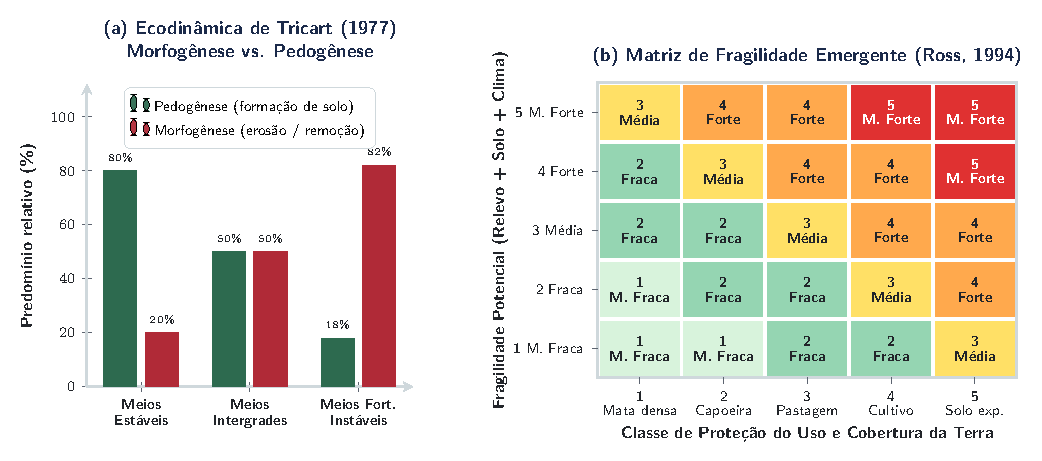
\includegraphics[width=0.95\textwidth]{figures/fig07_ecodinamica_ross_matriz.pdf}
  \caption{Integração metodológica entre a Ecodinâmica de Tricart (1977), expressa pelo balanço relativo entre pedogênese e morfogênese nos três tipos de meios ((a)), e a Matriz de Fragilidade Emergente de Ross (1994), obtida pelo cruzamento da Fragilidade Potencial com o grau de proteção do Uso da Terra ((b)).}
  \label{fig:ecodinamica_ross}
\end{figure}

\section{Análise Empírica da Fragilidade Ambiental (Ross, 1994)}

Na década de 1990, o geógrafo brasileiro \textbf{Jurandyr Luciano Sanches Ross (1994)} operacionalizou os princípios dos Geossistemas e da Ecodinâmica de Tricart em uma metodologia cartográfica e quantitativa padronizada: a \textbf{Análise Empírica da Fragilidade dos Ambientes Naturais e Antropizados}. Para manter a coerência com Tricart, Ross substituiu a expressão ``meios estáveis/instáveis'' por \textbf{Unidades Ecodinâmicas Estáveis} e \textbf{Unidades Ecodinâmicas de Instabilidade Potencial ou Emergente}, classificadas em \textbf{cinco graus hierárquicos}:
\[
  1 = \text{Muito Fraca} \quad;\quad 2 = \text{Fraca} \quad;\quad 3 = \text{Média} \quad;\quad 4 = \text{Forte} \quad;\quad 5 = \text{Muito Forte}.
\]

\begin{boxConceito}[Distinção Fundamental: Fragilidade Potencial vs. Fragilidade Emergente]
A \textbf{Fragilidade Potencial ($FP$)} expressa a suscetibilidade \emph{natural e intrínseca} do terreno antes de considerar a ação humana ou a vegetação atual, combinando exclusivamente os fatores do meio físico: \textbf{Relevo/Declividade ($D_R$)}, \textbf{Solos ($D_S$)} e \textbf{Clima/Pluviosidade ($D_C$)}. Ela responde à pergunta: \emph{``Quão vulnerável este terreno seria se perdesse sua cobertura vegetal?''} Já a \textbf{Fragilidade Emergente ($FE$)} traduz a suscetibilidade \emph{real e atual} do ambiente, resultando do cruzamento entre a \textbf{Fragilidade Potencial ($FP$)} e o grau de proteção oferecido pelo \textbf{Uso da Terra / Cobertura Vegetal ($D_U$)}, respondendo à questão: \emph{``Qual é o risco efetivo de degradação hoje, considerando o uso e a vegetação existentes?''}
\end{boxConceito}

\subsection{Tabelas Completas das Cinco Classes Hierárquicas de Ross (1994)}

As Tabelas~\ref{tab:ross_relevo_solos} e~\ref{tab:ross_clima_uso} apresentam os critérios completos das quatro variáveis básicas utilizadas na metodologia de Ross (1994). Em estudos de detalhe (microbacias e municípios, escalas de $1:10.000$ a $1:50.000$), adota-se a \textbf{declividade ($S\%$)} como indicador do relevo; em estudos regionais (escalas menores que $1:100.000$), utilizam-se os índices de dissecação do relevo (entalhamento de vales e dimensão interfluvial).

\begin{table}[H]
\centering
\caption{Classes hierárquicas de fragilidade para Relevo/Declividade ($D_R$) e Solos ($D_S$) segundo Ross (1994).}
\label{tab:ross_relevo_solos}
\renewcommand{\arraystretch}{1.18}
\small
\begin{tabularx}{\textwidth}{@{}p{1.9cm} p{2.9cm} p{3.5cm} >{\raggedright\arraybackslash}X@{}}
  \toprule
  \rowcolor{uefsNavy}
  \textcolor{white}{\bfseries Classe / Grau} & \textcolor{white}{\bfseries Declividade ($D_R$)} & \textcolor{white}{\bfseries Dissecação Regional ($D_R$)} & \textcolor{white}{\bfseries Classes de Solos / Erodibilidade ($D_S$)} \\
  \midrule
  \textbf{1, Muito Fraca} & $< 6\%$ & Muito fraca (vales muito rasos, interflúvios amplos) & Latossolos Roxos e Vermelho-Escuros de textura argilosa (muito profundos e bem estruturados). \\
  \rowcolor{bgGray}
  \textbf{2, Fraca} & $6\text{ a } 12\%$ & Fraca (entalhamento e densidade baixos) & Latossolos Vermelho-Amarelos de textura média/argilosa; Nitossolos profundos. \\
  \textbf{3, Média} & $12\text{ a } 20\%$ & Média (vertentes moderadamente dissecadas) & Latossolos Amarelos/Vermelho-Amarelos arenosos; Argissolos profundos; Cambissolos profundos. \\
  \rowcolor{bgGray}
  \textbf{4, Forte} & $20\text{ a } 30\%$ & Forte (vales entalhados e interflúvios estreitos) & Argissolos com mudança textural abrupta; Planossolos (comum no Semiárido); Cambissolos rasos/siltosos. \\
  \textbf{5, Muito Forte} & $> 30\%$ & Muito forte (escarpas, vales muito profundos) & Neossolos Litólicos (solos rasos sobre rocha), Neossolos Quartzarênicos (areias quartzosas), Gleissolos e Organossolos em áreas instáveis. \\
  \bottomrule
\end{tabularx}
\end{table}

Definidos os graus de vulnerabilidade intrínseca do relevo e dos solos na Tabela~\ref{tab:ross_relevo_solos}, o analista incorpora a agressividade climática (erosividade das chuvas) e o efeito protetor ou degradante da cobertura vegetal por meio dos critérios da Tabela~\ref{tab:ross_clima_uso}.

\begin{table}[H]
\centering
\caption{Classes hierárquicas de fragilidade para Clima/Pluviosidade ($D_C$) e Uso da Terra / Cobertura Vegetal ($D_U$) segundo Ross (1994).}
\label{tab:ross_clima_uso}
\renewcommand{\arraystretch}{1.18}
\small
\begin{tabularx}{\textwidth}{@{}p{1.9cm} p{5.5cm} >{\raggedright\arraybackslash}X@{}}
  \toprule
  \rowcolor{uefsNavy}
  \textcolor{white}{\bfseries Classe / Grau} & \textcolor{white}{\bfseries Clima / Pluviosidade ($D_C$, Erosividade)} & \textcolor{white}{\bfseries Uso da Terra / Cobertura Vegetal ($D_U$, Grau de Proteção)} \\
  \midrule
  \textbf{1, Muito Fraca} & Pluviosidade regular ao longo do ano, baixa intensidade horária, sem concentração extrema. & \textbf{Proteção Muito Alta:} florestas naturais primárias, matas ciliares densas e Caatinga arbórea fechada. \\
  \rowcolor{bgGray}
  \textbf{2, Fraca} & Precipitação moderada ($1.000\text{--}1.300\text{ mm/ano}$) com estação seca curta e chuvas pouco torrenciais. & \textbf{Proteção Alta:} florestas secundárias avançadas (capoeirões), Caatinga arbustivo-arbórea densa, silvicultura bem manejada. \\
  \textbf{3, Média} & Estação seca definida ($3\text{--}6$ meses) e chuvas concentradas no verão/outono com eventos erosivos moderados. & \textbf{Proteção Média:} pastagens bem manejadas com boa cobertura, sistemas agroflorestais (SAFs), culturas perenes (café, cacau em cabruca). \\
  \rowcolor{bgGray}
  \textbf{4, Forte} & Forte concentração pluviométrica sazonal (ou totais $>2.000\text{ mm/ano}$ com aguaceiros intensos). & \textbf{Proteção Baixa:} culturas temporárias de ciclo curto (milho, feijão, mandioca), pastagens degradadas/raleadas e áreas de queimada antiga. \\
  \textbf{5, Muito Forte} & Chuvas altamente concentradas e torrenciais (típico do Semiárido com aguaceiros sobre solo seco, ou áreas de extrema erosividade). & \textbf{Proteção Muito Baixa / Nula:} solo exposto, áreas terraplanadas, mineração, queimada recente, área urbana sem drenagem. \\
  \bottomrule
\end{tabularx}
\end{table}

\subsection{Cálculo e Leitura do Código Numérico de Ross ($FP$ e $FE$)}

Na metodologia de Ross (1994), cada unidade geoambiental recebe um \textbf{código numérico posicional} que preserva a memória individual de cada variável, impedindo que a causa do problema desapareça na média. O \textbf{Código da Fragilidade Potencial ($FP$)} é formado por \textbf{três dígitos} na ordem fixa $\mathbf{D_R\,D_S\,D_C}$ (Relevo, Solos e Clima), enquanto o \textbf{Código da Fragilidade Emergente ($FE$)} acrescenta o fator antrópico e passa a contar com \textbf{quatro dígitos} na ordem fixa $\mathbf{D_R\,D_S\,D_C\,D_U}$ (Relevo, Solos, Clima e Uso da Terra).

\begin{boxFormula}[Cálculo e Leitura da Fragilidade Potencial ($FP$) e Fragilidade Emergente ($FE$)]
\textbf{Passo 1, Atribuição dos dígitos ($1$ a $5$):} enquadre o terreno nas Tabelas~\ref{tab:ross_relevo_solos} e~\ref{tab:ross_clima_uso}, obtendo $D_R$, $D_S$, $D_C$ e $D_U$.

\textbf{Passo 2, Montagem dos códigos posicionais:}
\[
  \text{Código } FP = D_R\,D_S\,D_C \qquad\text{e}\qquad \text{Código } FE = D_R\,D_S\,D_C\,D_U.
\]

\textbf{Passo 3, Determinação da Classe Síntese de $FP$ (1 a 5):} calcula-se a média aritmética das três variáveis físicas e arredonda-se para o inteiro mais próximo de $1$ a $5$ (em empates de $0{,}5$, adota-se o valor mais conservador ou o peso dominante do relevo $D_R$):
\[
  I_{FP} = \frac{D_R + D_S + D_C}{3} \quad \xrightarrow{\text{arredondamento}} \quad \text{Classe } FP \in \{1, 2, 3, 4, 5\}.
\]

\textbf{Passo 4, Determinação da Classe Síntese de $FE$ (1 a 5) na Matriz de Fragilidade Emergente:} cruza-se a \textbf{Classe $FP$} (linha) com o dígito do \textbf{Uso da Terra $D_U$} (coluna) na adaptação didático-operacional da matriz de Ross (1994) e Spörl e Ross (2004) apresentada abaixo (Figura~\ref{fig:ecodinamica_ross}, (b)). Nos casos em que $(FP + D_U)/2$ resulta em fração $0{,}5$, a matriz pondera o efeito protetor da cobertura vegetal densa ($D_U \le 2$, arredondando para baixo) em contraste com o agravamento imposto por usos antrópicos expostos ($D_U \ge 3$, arredondando para cima):

\begin{center}
\renewcommand{\arraystretch}{1.12}
\footnotesize
\begin{tabular}{@{}l|ccccc@{}}
  \toprule
  \textbf{Fragilidade Potencial ($FP$)} $\backslash$ \textbf{Uso ($D_U$)} & \textbf{1 (M. Alta Prot.)} & \textbf{2 (Alta)} & \textbf{3 (Média)} & \textbf{4 (Baixa)} & \textbf{5 (Nula)} \\
  \midrule
  \textbf{1, Muito Fraca} & 1 (M. Fraca) & 1 (M. Fraca) & 2 (Fraca) & 2 (Fraca) & 3 (Média) \\
  \textbf{2, Fraca} & 1 (M. Fraca) & 2 (Fraca) & 2 (Fraca) & 3 (Média) & 4 (Forte) \\
  \textbf{3, Média} & 2 (Fraca) & 2 (Fraca) & 3 (Média) & 4 (Forte) & 4 (Forte) \\
  \textbf{4, Forte} & 2 (Fraca) & 3 (Média) & 4 (Forte) & 4 (Forte) & 5 (M. Forte) \\
  \textbf{5, Muito Forte} & 3 (Média) & 4 (Forte) & 4 (Forte) & 5 (M. Forte) & 5 (M. Forte) \\
  \bottomrule
\end{tabular}
\end{center}
\vspace{2pt}
{\footnotesize\emph{Nota:} na célula $(FP=5, D_U=1)$, a proteção florestal primária reduz a fragilidade emergente para \textbf{3, Média}.}

\textbf{Exemplo numérico completo:} considere uma encosta com declividade $S = 22\%$ ($D_R = 4$), Argissolo profundo ($D_S = 3$), clima semiárido com chuvas torrenciais concentradas ($D_C = 4$) e pastagem degradada ($D_U = 4$). O \textbf{Código $FP$} resulta em $\mathbf{434}$, cuja média $I_{FP} = (4 + 3 + 4)/3 = 11/3 \approx 3{,}67$ conduz à \textbf{Classe $FP = 4$ (Forte)}. Ao incorporar o uso atual, obtém-se o \textbf{Código $FE$} igual a $\mathbf{4344}$, e o cruzamento de $FP = 4$ com $D_U = 4$ na matriz acima confirma a \textbf{Classe $FE = 4$ (Forte)}. Na leitura técnica do código $4344$, o primeiro dígito ($4$) alerta que a declividade ($20\text{--}30\%$) é o principal motor físico da instabilidade, o terceiro dígito ($4$) indica forte erosividade climática, e o quarto dígito ($4$) revela que a pastagem degradada deixa o solo desprotegido, mantendo o risco real elevado (Classe 4).
\end{boxFormula}

\etapa{4}{Estudos de Caso e Exemplos Resolvidos}

\begin{boxExemplo}{9.1}{Enquadramento na Taxonomia da Paisagem de Bertrand (Nível Básico)}
\passoEnunciado{Uma equipe de Análise Ambiental da UEFS está diagnosticando processos erosivos em uma propriedade rural próxima a Feira de Santana (BA). Durante o trabalho, os estudantes precisam situar espacialmente quatro recortes: (I) o Domínio das Caatingas; (II) a sub-bacia do Rio Jacuípe (escala $1:100.000$); (III) uma vertente homogênea de pastagem sobre Argissolo ($1:15.000$); e (IV) uma voçoroca ativa com $40\,\text{m}$ de comprimento ($1:1.000$).}
\passoDados{Quatro recortes espaciais com escalas variando de continental/regional ($G\text{II}$) até o detalhe local ($G\text{VII}$).}
\passoPedido{Enquadrar corretamente cada recorte (I a IV) nas unidades taxonômicas de Bertrand (2004).}
\passoMetodo{Aplicação direta da Tabela~\ref{tab:taxonomia_bertrand} (unidades superiores e inferiores segundo ordem de grandeza e critério definidor).}
\passoContas{%
\begin{enumerate}[leftmargin=1.6em, itemsep=1.5pt]
  \item \textbf{Recorte I (Domínio das Caatingas):} escala regional/subcontinental ($G\text{II}$, $\sim 10^6\text{ km}^2$) definida por macroclima e bioma $\implies$ \textbf{Domínio}.
  \item \textbf{Recorte II (Sub-bacia em $1:100.000$):} unidade funcional concreta ($G\text{V}$, dezenas a centenas de $\text{km}^2$) que integra potencial ecológico, exploração biológica e ação antrópica $\implies$ \textbf{Geossistema}.
  \item \textbf{Recorte III (Vertente homogênea em $1:15.000$):} setor fisionomicamente uniforme dentro do geossistema ($G\text{VI}$) $\implies$ \textbf{Geofácies}.
  \item \textbf{Recorte IV (Voçoroca de $40\,\text{m}$ em $1:1.000$):} menor unidade espacial de detalhe extremo ($G\text{VII}$) $\implies$ \textbf{Geótopo}.
\end{enumerate}}
\passoResposta{I = Domínio; II = Geossistema; III = Geofácies; IV = Geótopo.}
\passoVerificacao{A sequência segue exatamente a ordem decrescente de grandeza espacial da taxonomia de Bertrand ($G\text{II} \to G\text{V} \to G\text{VI} \to G\text{VII}$), evitando misturar unidades regionais com feições pontuais de campo.}
\end{boxExemplo}

\begin{boxExemplo}{9.2}{Diagnóstico Ecodinâmico de Tricart em Três Setores de Sub-bacia (Nível Básico–Intermediário)}
\passoEnunciado{Ao percorrer uma sub-bacia do Piemonte da Chapada Diamantina, um geógrafo observou três compartimentos distintos: \textbf{Setor X}, chapada plana com vegetação arbórea conservada, Latossolo profundo e ausência de sulcos; \textbf{Setor Y}, rampa suave ($9\%$) com pastagem manejada, onde ocorrem infiltração moderada e leve escoamento laminar após chuvas fortes; \textbf{Setor Z}, encosta íngreme ($35\%$) desmatada, com Neossolo Litólico raso, ravinas profundas e blocos rolados.}
\passoDados{Setor X (plano, florestado, solo profundo); Setor Y ($S=9\%$, pastagem, erosão laminar leve); Setor Z ($S=35\%$, desmatado, solo raso, ravinas).}
\passoPedido{Classificar cada setor segundo a Ecodinâmica de Tricart (1977), explicando o balanço morfogênese vs. pedogênese.}
\passoMetodo{Comparação dos processos dominantes com os critérios da Tabela~\ref{tab:ecodinamica_tricart} e do (a) da Figura~\ref{fig:ecodinamica_ross}.}
\passoContas{%
\begin{enumerate}[leftmargin=1.6em, itemsep=1.5pt]
  \item \textbf{Setor X:} a cobertura arbórea e o relevo plano maximizam a infiltração e o intemperismo químico profundo, bloqueando a erosão superficial ($P \gg M$) $\implies$ \textbf{Meio Estável}.
  \item \textbf{Setor Y:} há competição equilibrada entre infiltração sob pastagem e remoção laminar nas chuvas intensas ($P \approx M$) $\implies$ \textbf{Meio Intergrade (de Transição)}.
  \item \textbf{Setor Z:} a alta declividade aliada à remoção da vegetação dispara erosão linear e perda acelerada de solo ($M \gg P$) $\implies$ \textbf{Meio Fortemente Instável}.
\end{enumerate}}
\passoResposta{Setor X = Meio Estável; Setor Y = Meio Intergrade; Setor Z = Meio Fortemente Instável.}
\passoVerificacao{O diagnóstico orienta diretamente a gestão: no Setor Z a prioridade é contenção erosiva e revegetação; no Setor Y, manejo conservacionista para impedir que o meio intergrade migre para a instabilidade forte.}
\end{boxExemplo}

\begin{boxExemplo}{9.3}{Cálculo Passo a Passo da Fragilidade Potencial e Emergente (Nível Intermediário)}
\passoEnunciado{Uma unidade geoambiental utilizada para estudo de planejamento municipal apresenta declividade média de $S = 15\%$, solo classificado como Argissolo profundo de textura média/argilosa, clima tropical semiárido com chuvas concentradas e torrenciais ($D_C = 4$) e uso atual por cultura temporária de mandioca em solo parcialmente descoberto.}
\passoDados{$S = 15\%$; Argissolo profundo; $D_C = 4$; uso por cultura temporária de ciclo curto.}
\passoPedido{Determinar os dígitos $D_R$, $D_S$, $D_C$ e $D_U$, montar os códigos numéricos de $FP$ e $FE$ e obter as classes síntese de Fragilidade Potencial e Emergente.}
\passoMetodo{Enquadramento pelas Tabelas~\ref{tab:ross_relevo_solos} e~\ref{tab:ross_clima_uso} e aplicação do roteiro de cálculo de Ross (1994).}
\passoContas{%
\begin{enumerate}[leftmargin=1.6em, itemsep=1.5pt]
  \item \textbf{Atribuição dos dígitos:}
  \begin{itemize}[leftmargin=1.4em, itemsep=1pt]
    \item Relevo ($S = 15\%$, faixa $12\text{--}20\%$): $D_R = 3$ (Média).
    \item Solos (Argissolo profundo): $D_S = 3$ (Média).
    \item Clima (fornecido): $D_C = 4$ (Forte).
    \item Uso da Terra (cultura temporária de ciclo curto): $D_U = 4$ (Proteção Baixa / Fragilidade Forte).
  \end{itemize}
  \item \textbf{Fragilidade Potencial ($FP$):} código posicional $\mathbf{334}$. Média física:
  \[
    I_{FP} = \frac{3 + 3 + 4}{3} = \frac{10}{3} \approx 3{,}33 \implies \text{Classe } FP = \mathbf{3\text{ (Média)}}.
  \]
  \item \textbf{Fragilidade Emergente ($FE$):} código posicional $\mathbf{3344}$. Cruzando $FP = 3$ com $D_U = 4$ na Matriz de Ross (Figura~\ref{fig:ecodinamica_ross}, (b)) $\implies$ \textbf{Classe $FE = 4$ (Forte)}.
\end{enumerate}}
\passoResposta{Código $FP = 334$ (Classe 3, Média); Código $FE = 3344$ (Classe 4, Forte).}
\passoVerificacao{Note o papel agravante do uso agrícola anual ($D_U = 4$): a unidade possui fragilidade natural média ($3$), mas o cultivo temporário com baixa proteção eleva a fragilidade real emergente para forte ($4$), exigindo plantio em nível e cobertura morta.}
\end{boxExemplo}

\begin{boxExemplo}{9.4}{Efeito Amortecedor da Vegetação na Matriz de Ross (Nível Intermediário–Avançado)}
\passoEnunciado{Considere uma encosta íngreme de $S = 24\%$ ($D_R = 4$) com Planossolo/Argissolo abrúptico ($D_S = 4$) sob regime de chuvas intensas sazonais ($D_C = 4$). Compare dois cenários de uso sobre essa mesma base física: \textbf{Cenário 1}, área mantida com mata nativa primária densa; \textbf{Cenário 2}, área totalmente desmatada e terraplanada (solo exposto) para loteamento sem drenagem.}
\passoDados{$D_R = 4$, $D_S = 4$, $D_C = 4$. Cenário 1: mata primária densa. Cenário 2: solo exposto/terraplanagem.}
\passoPedido{Calcular $FP$ e $FE$ para ambos os cenários e explicar tecnicamente a diferença obtida.}
\passoMetodo{Cálculo do código $FP$, identificação de $D_U$ pela Tabela~\ref{tab:ross_clima_uso} e leitura da Matriz de Fragilidade Emergente de Ross.}
\passoContas{%
\begin{enumerate}[leftmargin=1.6em, itemsep=1.5pt]
  \item \textbf{Fragilidade Potencial ($FP$, idêntica nos dois cenários):} código $\mathbf{444}$; $I_{FP} = (4+4+4)/3 = 4{,}0 \implies$ \textbf{Classe $FP = 4$ (Forte)}.
  \item \textbf{Cenário 1 (mata nativa densa $\implies D_U = 1$):} código $FE = \mathbf{4441}$. Na Matriz de Ross, o cruzamento $FP = 4 \times D_U = 1$ resulta em \textbf{Classe $FE = 2$ (Fraca)}.
  \item \textbf{Cenário 2 (solo exposto $\implies D_U = 5$):} código $FE = \mathbf{4445}$. Na Matriz de Ross, o cruzamento $FP = 4 \times D_U = 5$ resulta em \textbf{Classe $FE = 5$ (Muito Forte)}.
\end{enumerate}}
\passoResposta{Ambos têm $FP = 444$ (Classe 4, Forte). No Cenário 1, $FE = 4441$ (Classe 2, Fraca); no Cenário 2, $FE = 4445$ (Classe 5, Muito Forte).}
\passoVerificacao{O resultado comprova quantitativamente o princípio de Ross e Tricart: a floresta densa reduz em dois graus a fragilidade emergente ($4 \to 2$), mantendo o equilíbrio pedogenético; já a exposição do solo libera toda a energia potencial da encosta, disparando a fragilidade máxima ($5$).}
\end{boxExemplo}

\begin{boxExemplo}{9.5}{Compartimentação Geoambiental e Zoneamento de Microbacia (Nível Avançado)}
\passoEnunciado{Para elaborar o diagnóstico físico-ambiental do Trabalho Prático Final, uma microbacia do Semiárido baiano ($D_C = 4$ em toda a área) foi compartimentada em três Unidades Geoambientais (UGs):
\begin{itemize}[leftmargin=1.4em, itemsep=1pt]
  \item \textbf{UG1 (Topo de Tabuleiro):} $S = 3\%$, Latossolo Vermelho-Escuro argiloso, Caatinga arbustivo-arbórea densa;
  \item \textbf{UG2 (Meia Encosta Dissecada):} $S = 35\%$, Neossolo Litólico, pastagem degradada;
  \item \textbf{UG3 (Sopé Coluvial):} $S = 9\%$, Planossolo, sistema agroflorestal (SAF) manejado.
\end{itemize}}
\passoDados{UG1 ($S=3\%$, Latossolo argiloso, Caatinga densa); UG2 ($S=35\%$, Neossolo Litólico, pastagem degradada); UG3 ($S=9\%$, Planossolo, SAF manejado); $D_C = 4$ em toda a microbacia.}
\passoPedido{Calcular o código $FP$, a classe $FP$, o código $FE$, a classe $FE$ e o meio ecodinâmico de Tricart para cada UG, propondo diretrizes de ordenamento.}
\passoMetodo{Integração das Tabelas~\ref{tab:ecodinamica_tricart}, \ref{tab:ross_relevo_solos} e~\ref{tab:ross_clima_uso} e da Matriz de Ross.}
\passoContas{%
\begin{enumerate}[leftmargin=1.6em, itemsep=1.5pt]
  \item \textbf{UG1 (Topo):} $D_R=1$, $D_S=1$, $D_C=4$, $D_U=2$. Código $FP = \mathbf{114}$, $I_{FP} = (1+1+4)/3 = 2{,}0 \implies FP = \mathbf{2}$ (Fraca). Código $FE = \mathbf{1142}$; cruzando $FP=2 \times D_U=2 \implies FE = \mathbf{2}$ (Fraca). Meio \textbf{Estável}.
  \item \textbf{UG2 (Meia Encosta):} $D_R=5$, $D_S=5$, $D_C=4$, $D_U=4$. Código $FP = \mathbf{554}$, $I_{FP} = (5+5+4)/3 = 14/3 \approx 4{,}67 \implies FP = \mathbf{5}$ (Muito Forte). Código $FE = \mathbf{5544}$; cruzando $FP=5 \times D_U=4 \implies FE = \mathbf{5}$ (Muito Forte). Meio \textbf{Fortemente Instável}.
  \item \textbf{UG3 (Sopé):} $D_R=2$, $D_S=4$, $D_C=4$, $D_U=3$. Código $FP = \mathbf{244}$, $I_{FP} = (2+4+4)/3 = 10/3 \approx 3{,}33 \implies FP = \mathbf{3}$ (Média). Código $FE = \mathbf{2443}$; cruzando $FP=3 \times D_U=3 \implies FE = \mathbf{3}$ (Média). Meio \textbf{Intergrade}.
\end{enumerate}}
\passoResposta{UG1: $FP=114$ (2), $FE=1142$ (2, Fraca, Estável); UG2: $FP=554$ (5), $FE=5544$ (5, Muito Forte, Fortemente Instável); UG3: $FP=244$ (3), $FE=2443$ (3, Média, Intergrade).}
\passoVerificacao{O zoneamento resultante é ambientalmente coerente: UG1 comporta uso sustentável controlado; UG3 exige manejo conservacionista (manutenção do SAF e drenagem do Planossolo); UG2 deve ser destinada à preservação e recuperação (exclusão do gado e bioengenharia para conter ravinas).}
\end{boxExemplo}

\etapa{5}{Erros Mais Comuns em Provas e Diagnósticos}

\begin{boxErro}[Erro 1: Confundir Fragilidade Potencial ($FP$) com Fragilidade Emergente ($FE$)]
\textbf{Equívoco frequente:} incluir o uso da terra ($D_U$) no cálculo da Fragilidade Potencial, ou afirmar que uma encosta íngreme florestada tem ``baixa fragilidade potencial''.

\textbf{Correção técnica:} a \textbf{Fragilidade Potencial ($FP$)} depende exclusivamente dos fatores físicos naturais ($D_R, D_S, D_C$). Uma encosta de $35\%$ com solo raso continua tendo \textbf{FP Muito Forte ($5$)} mesmo sob mata primária; o que a floresta reduz é a \textbf{Fragilidade Emergente ($FE$)}, que passa a depender do uso atual ($D_U$).
\end{boxErro}

\begin{boxErro}[Erro 2: Inverter a escala de proteção do Uso da Terra ($D_U$) em Ross (1994)]
\textbf{Equívoco frequente:} atribuir classe $5$ para floresta densa (por associar $5$ ao ``máximo de vegetação'') e classe $1$ para solo exposto.

\textbf{Correção técnica:} na metodologia de Ross, \textbf{todas as variáveis seguem o sentido da fragilidade} ($1$ = menor fragilidade; $5$ = maior fragilidade). Portanto, a floresta densa, por oferecer máxima proteção contra a erosão, recebe \textbf{classe $1$}, enquanto o solo exposto recebe \textbf{classe $5$}.
\end{boxErro}

\begin{boxErro}[Erro 3: Tratar ``Meio Intergrade'' como sinônimo de ``Meio Sem Risco'']
\textbf{Equívoco frequente:} concluir que ambientes intergrades de Tricart são estáveis e dispensam práticas de manejo.

\textbf{Correção técnica:} o meio intergrade é uma \textbf{zona de transição dinâmica} ($P \approx M$). Basta uma intervenção inadequada (queimada, sobrepastejo ou corte de talude) para que a morfogênese supere a pedogênese e o setor passe rapidamente a fortemente instável.
\end{boxErro}

\begin{boxErro}[Erro 4: Usar Geossistema e Ecossistema como termos idênticos sem critério escalar]
\textbf{Equívoco frequente:} chamar qualquer parcela de $10\text{ m}^2$ ou um bioma continental inteiro de ``geossistema''.

\textbf{Correção técnica:} na taxonomia de Bertrand (2004), o geossistema ocupa a ordem $G\text{V}$ (escala de dezenas a centenas de $\text{km}^2$, cartas de $1:50.000$ a $1:100.000$). Unidades continentais pertencem à Zona/Domínio ($G\text{I}\text{--}G\text{II}$), e unidades pontuais de campo pertencem ao Geótopo ($G\text{VII}$).
\end{boxErro}

\etapa{6}{Exercícios de Fixação}

\subsection*{Nível Básico (Exercícios 1 a 5)}

\begin{enumerate}[leftmargin=1.8em, itemsep=4pt]
  \item Explique, com base na Teoria Geral dos Sistemas (Bertalanffy, 2010), por que a fragilidade ambiental é considerada uma \textbf{propriedade emergente} da paisagem e não uma característica isolada de um único elemento físico.
  \espacoResolucao[1.8cm]

  \item Liste em ordem decrescente de escala espacial as seis unidades taxonômicas da paisagem propostas por Bertrand (2004), separando as unidades superiores das unidades inferiores.
  \espacoResolucao[1.8cm]

  \item Defina \textbf{morfogênese} e \textbf{pedogênese} segundo Tricart (1977) e indique qual processo predomina nos meios estáveis e nos meios fortemente instáveis.
  \espacoResolucao[1.8cm]

  \item Um terreno possui $D_R = 2$ (declividade $8\%$), $D_S = 2$ (Latossolo Vermelho-Amarelo argiloso) e $D_C = 2$. Calcule o código numérico e a classe da \textbf{Fragilidade Potencial ($FP$)}.
  \espacoResolucao[1.6cm]

  \item Por que a floresta primária densa recebe dígito $D_U = 1$ e o solo exposto recebe dígito $D_U = 5$ na tabela de Ross (1994)?
  \espacoResolucao[1.6cm]
\end{enumerate}

\subsection*{Nível Intermediário (Exercícios 6 a 10)}

\begin{enumerate}[leftmargin=1.8em, itemsep=4pt, resume]
  \item Uma unidade geoambiental apresenta $S = 25\%$, Planossolo ($D_S = 4$), clima semiárido com chuvas torrenciais ($D_C = 4$) e uso atual com pastagem bem manejada ($D_U = 3$). Determine os códigos numéricos e as classes de $FP$ e $FE$.
  \espacoResolucao[2.0cm]

  \item Considere duas áreas vizinhas com mesma Fragilidade Potencial ($FP = 343$, Classe 3, Média): a Área A possui Caatinga arbórea densa ($D_U = 1$) e a Área B sofreu corte raso e queimada recente ($D_U = 5$). Calcule $FE$ para ambas e interprete a diferença à luz da Ecodinâmica de Tricart.
  \espacoResolucao[2.2cm]

  \item Explique a diferença conceitual e prática entre \textbf{Geossistema}, \textbf{Geofácies} e \textbf{Geótopo}, dando um exemplo de cada um em uma bacia hidrográfica do Semiárido baiano.
  \espacoResolucao[2.0cm]

  \item Uma encosta com $S = 14\%$, Neossolo Litólico ($D_S = 5$) e $D_C = 3$ é utilizada para cultivo temporário de milho ($D_U = 4$). Determine $FP$ e $FE$ e explique por que o dígito $5$ do solo exige atenção especial mesmo quando a média $I_{FP}$ é intermediária.
  \espacoResolucao[2.0cm]

  \item Como a \textbf{compartimentação geoambiental} (Rodriguez; Silva; Cavalcanti, 2017) transforma a análise teórica de geossistemas em instrumento prático para o Zoneamento Ecológico-Econômico (ZEE)?
  \espacoResolucao[2.0cm]
\end{enumerate}

\subsection*{Questões Objetivas (Exercícios 11 a 15)}

\begin{enumerate}[leftmargin=1.8em, itemsep=5pt, resume]
  \item Na taxonomia da paisagem de Bertrand (2004), uma unidade territorial de escala $1:50.000$ definida pela interação dinâmica entre potencial ecológico, exploração biológica e ação antrópica denomina-se:
  \begin{alternativas}
    \item Zona.
    \item Domínio.
    \item Geossistema.
    \item Geótopo.
    \item Bioma zonal.
  \end{alternativas}

  \item Segundo a Ecodinâmica de Tricart (1977), um ambiente com vegetação densa, relevo suave, solos profundos e predomínio nítido da infiltração e formação de solo sobre a erosão classifica-se como:
  \begin{alternativas}
    \item Meio fortemente instável.
    \item Meio estável.
    \item Meio degradado irreversível.
    \item Meio estritamente morfogenético.
    \item Meio abiótico residual.
  \end{alternativas}

  \item Na metodologia de Ross (1994), uma unidade com declividade de $22\%$ ($D_R = 4$), Argissolo abrúptico ($D_S = 4$), clima com chuvas concentradas ($D_C = 4$) e cobertura florestal primária ($D_U = 1$) possui:
  \begin{alternativas}
    \item Código $FP = 444$ (Classe 4, Forte) e código $FE = 4441$ (Classe 2, Fraca).
    \item Código $FP = 111$ (Classe 1, Muito Fraca) e código $FE = 1114$ (Classe 4, Forte).
    \item Código $FP = 444$ (Classe 4, Forte) e código $FE = 4441$ (Classe 5, Muito Forte).
    \item Código $FP = 441$ (Classe 3, Média) e código $FE = 4411$ (Classe 1, Muito Fraca).
    \item Código $FP = 555$ (Classe 5, Muito Forte) e código $FE = 5555$ (Classe 5, Muito Forte).
  \end{alternativas}

  \item Sobre as cinco classes de Uso da Terra e Cobertura Vegetal ($D_U$) propostas por Ross (1994), é correto afirmar que:
  \begin{alternativas}
    \item Quanto maior a densidade e a proteção da cobertura vegetal, maior é o número atribuído à classe ($5$ para floresta).
    \item Culturas temporárias de ciclo curto e solo exposto recebem classes baixas ($1$ e $2$) por terem menor biomassa.
    \item A classe $1$ corresponde à proteção muito alta (florestas densas) e a classe $5$ corresponde à proteção muito baixa ou nula (solo exposto).
    \item O uso da terra entra exclusivamente no cálculo da Fragilidade Potencial ($FP$).
    \item Pastagens degradadas conferem proteção superior à das florestas primárias.
  \end{alternativas}

  \item O código numérico posicional adotado por Ross (1994), como $5545$, é preferível a uma nota média única sem código porque:
  \begin{alternativas}
    \item Permite identificar qual fator específico (relevo, solo, clima ou uso) é o principal responsável pela fragilidade da unidade.
    \item Dispensa qualquer mapeamento de declividade ou de solos em SIG.
    \item Garante que todas as unidades tenham sempre o mesmo valor de fragilidade.
    \item Substitui a legislação ambiental e o licenciamento de obras.
    \item Elimina a necessidade de trabalho de campo na Análise Ambiental.
  \end{alternativas}
\end{enumerate}

\etapa{7}{Questões de Provas, ENADE e Concursos Ambientais}

\begin{enumerate}[leftmargin=1.8em, itemsep=5pt, start=16]
  \item \textbf{(Questão autoral, estilo ENADE / Geografia)} A concepção sistêmica aplicada à análise da paisagem (Bertalanffy, 2010; Bertrand, 2004) superou a abordagem setorial clássica da Geografia Física. Nessa perspectiva integrada, o conceito de \textbf{geossistema} destaca-se metodologicamente porque:
  \begin{alternativas}
    \item Analisa apenas a geologia estrutural, desconsiderando a cobertura vegetal e a ação humana.
    \item Integra o potencial ecológico (meio físico), a exploração biológica (solos e biota) e a ação antrópica em uma unidade espacial concreta e cartografável.
    \item Aplica-se exclusivamente a ambientes polares e desérticos sem ocupação humana.
    \item Reduz a dinâmica ambiental a fenômenos puramente econômicos, sem base geomorfológica.
    \item Confunde-se com o geótopo por possuir área inferior a alguns metros quadrados.
  \end{alternativas}

  \needspace{5\baselineskip}
  \item \textbf{(Questão autoral, estilo Concurso Analista Ambiental / Planejamento Territorial)} Em um estudo de Fragilidade Ambiental segundo Ross (1994), um município identificou duas áreas de mesma \textbf{Fragilidade Potencial Forte ($FP = 4$)}. A Área 1 permanece coberta por mata nativa conservada ($D_U = 1$), enquanto a Área 2 foi convertida em solo exposto para extração mineral irregular ($D_U = 5$). Comparando os dois casos na Matriz de Ross, conclui-se corretamente que:
  \begin{alternativas}
    \item A Área 1 apresenta Fragilidade Emergente Fraca ($FE = 2$) devido ao efeito protetor da floresta, enquanto a Área 2 atinge Fragilidade Emergente Muito Forte ($FE = 5$).
    \item A Área 1 apresenta $FE = 5$ por ter maior biomassa, enquanto a Área 2 tem $FE = 1$.
    \item Ambas possuem $FE = 4$, pois o uso da terra não altera a fragilidade emergente.
    \item A Área 1 perdeu sua fragilidade potencial natural ao ser protegida por lei.
    \item O código numérico da Área 2 deve ser invertido para priorizar a mineração.
  \end{alternativas}

  \item \textbf{(Questão autoral, estilo Concurso Perito Ambiental / Ecodinâmica)} Durante uma perícia em encosta rural ocupada por pecuária extensiva sobre Neossolos Litólicos ($S = 28\%$), verificou-se remoção intensa do horizonte superficial, ravinamento ativo e exposição de fragmentos rochosos, com perda quase total da capacidade de formação de novo solo. À luz de Tricart (1977), essa área encontra-se em:
  \begin{alternativas}
    \item Meio estável, com amplo predomínio da pedogênese sobre a morfogênese.
    \item Meio fortemente instável, com nítido predomínio da morfogênese sobre a pedogênese.
    \item Equilíbrio climático estático, sem risco de perda produtiva ou assoreamento.
    \item Estágio de pedogênese acelerada favorável ao pisoteio bovino intensivo.
    \item Unidade zonal de escala $G\text{I}$ imune a intervenções locais de manejo.
  \end{alternativas}
\end{enumerate}

\begin{boxDica}[Conexão Direta com a Avaliação Teórica (Semana 10) e com o Trabalho Prático Final]
Você completou o \textbf{Módulo 3}! Na Semana 10, a Avaliação Teórica cobrará exatamente a articulação entre os fundamentos socioambientais (Módulo 1), a AIA e os sistemas abertos (Módulo 2) e o tripé técnico-geográfico \textbf{Bacias + Morfopedologia + Geossistemas/Tricart/Ross} (Módulo 3). Use o \textbf{Simulado Preparatório} logo após este capítulo como treino integral em condições reais de prova!
\end{boxDica}

\clearpage
\etapa{8}{Gabarito Comentado: Exercícios 1 a 18}

\begin{boxGabarito}[Resoluções e Justificativas: Capítulo 9]
\begin{enumerate}[leftmargin=1.8em, itemsep=3.5pt]
  \item \textbf{Propriedade emergente (TGS):} a fragilidade ambiental resulta da interação simultânea entre relevo, solo, clima e cobertura vegetal/uso da terra. Nenhum elemento isolado define o risco final; uma declividade alta pode ser estabilizada por floresta densa, enquanto um solo frágil em clima torrencial degrada-se ao perder a vegetação.

  \item \textbf{Taxonomia de Bertrand (2004):} \emph{Unidades superiores:} (1) Zona, (2) Domínio, (3) Região Natural. \emph{Unidades inferiores:} (4) Geossistema, (5) Geofácies, (6) Geótopo.

  \item \textbf{Tricart (1977):} \emph{pedogênese} é o conjunto de processos que formam e aprofundam o solo; \emph{morfogênese} engloba os processos erosivos e de remoção que modelam o relevo. Nos \textbf{meios estáveis} predomina a pedogênese ($P \gg M$); nos \textbf{meios fortemente instáveis} predomina a morfogênese ($M \gg P$).

  \item \textbf{Cálculo de $FP$:} código $FP = \mathbf{222}$. Média $I_{FP} = (2+2+2)/3 = 2{,}0 \implies$ \textbf{Classe $FP = 2$ (Fraca)}.

  \item \textbf{Sentido da escala de Ross:} em Ross (1994), a escala numérica de $1$ a $5$ mede sempre o \textbf{grau de fragilidade} (de Muito Fraca a Muito Forte). Como a floresta densa protege maximamente o solo contra o impacto da chuva e o escoamento, ela gera a menor fragilidade ($D_U = 1$); o solo exposto oferece proteção nula, gerando a maior fragilidade ($D_U = 5$).

  \item \textbf{Cálculo completo ($S=25\%$, Planossolo, $D_C=4$, pastagem manejada):} $D_R=4$ ($20\text{--}30\%$), $D_S=4$, $D_C=4$, $D_U=3$. Código $FP = \mathbf{444}$, $I_{FP} = (4+4+4)/3 = 4{,}0 \implies$ \textbf{Classe $FP = 4$ (Forte)}. Código $FE = \mathbf{4443}$; cruzando $FP=4 \times D_U=3$ na Matriz de Ross $\implies$ \textbf{Classe $FE = 4$ (Forte)}.

  \item \textbf{Comparação Área A vs. Área B ($FP = 343$, Classe 3):}
  \begin{itemize}[leftmargin=1.4em, itemsep=1pt]
    \item \textbf{Área A ($D_U=1$):} $FE = \mathbf{3431} \implies$ cruzando $FP=3 \times D_U=1$ na matriz resulta \textbf{Classe $FE = 2$ (Fraca)}, comportamento próximo ao meio estável/intergrade protegido.
    \item \textbf{Área B ($D_U=5$):} $FE = \mathbf{3435} \implies$ cruzando $FP=3 \times D_U=5$ na matriz resulta \textbf{Classe $FE = 4$ (Forte)}, ruptura do equilíbrio dinâmico, migrando para forte instabilidade morfogenética.
  \end{itemize}

  \item \textbf{Diferenciação escalar no Semiárido:} \emph{Geossistema} ($1:50.000\text{--}1:100.000$): uma sub-bacia do Semiárido com suas serras, depressões e usos rurais; \emph{Geofácies} ($1:10.000\text{--}1:25.000$): uma meia encosta homogênea com Caatinga arbustiva sobre Neossolo; \emph{Geótopo} ($>1:5.000$): uma voçoroca ativa ou lajedo específico dentro dessa encosta.

  \item \textbf{Cálculo ($S=14\%$, Neossolo Litólico, $D_C=3$, milho):} $D_R=3$, $D_S=5$, $D_C=3$, $D_U=4$. Código $FP = \mathbf{353}$, $I_{FP} = (3+5+3)/3 = 11/3 \approx 3{,}67 \implies$ \textbf{Classe $FP = 4$ (Forte)}. Código $FE = \mathbf{3534}$; cruzando $FP=4 \times D_U=4 \implies$ \textbf{Classe $FE = 4$ (Forte)}. O dígito $5$ em $D_S$ alerta que o solo é muito raso (Neossolo Litólico), logo qualquer perda erosiva expõe rapidamente a rocha.

  \item \textbf{Compartimentação e ZEE:} ao delimitar unidades geoambientais homogêneas (em termos de relevo, solo, clima, ecodinâmica e uso), a compartimentação fornece a base cartográfica direta para definir zonas de preservação, recuperação ou uso produtivo sustentável no ZEE.

  \item \textbf{Gabarito: (C).} O Geossistema corresponde à unidade de ordem $G\text{V}$ (escala $1:50.000$ a $1:100.000$) que sintetiza potencial ecológico, exploração biológica e ação antrópica.

  \item \textbf{Gabarito: (B).} Predomínio da pedogênese sobre a morfogênese sob vegetação densa e relevo suave define o Meio Estável de Tricart (1977).

  \item \textbf{Gabarito: (A).} $D_R=4, D_S=4, D_C=4 \implies FP = 444$ (Classe 4, Forte). Com mata primária ($D_U=1$), $FE = 4441$ e o cruzamento $4 \times 1$ na Matriz de Ross resulta em Classe 2, Fraca.

  \item \textbf{Gabarito: (C).} Em Ross (1994), $1$ indica menor fragilidade (proteção muito alta da floresta) e $5$ indica maior fragilidade (proteção nula do solo exposto).

  \item \textbf{Gabarito: (A).} A notação posicional mantém visível a contribuição individual de cada fator ($D_R, D_S, D_C, D_U$), orientando ações corretivas específicas.

  \item \textbf{Gabarito: (B).} Bertrand (2004) concebe o geossistema como unidade territorial concreta e cartografável resultante da interação entre fatores abióticos, bióticos e antrópicos.

  \item \textbf{Gabarito: (A).} Na Matriz de Fragilidade Emergente de Ross (Figura~\ref{fig:ecodinamica_ross}, (b)), $FP=4 \times D_U=1 \implies FE=2$ (Fraca), enquanto $FP=4 \times D_U=5 \implies FE=5$ (Muito Forte).

  \item \textbf{Gabarito: (B).} Declividade acentuada ($28\%$), solo raso (Neossolo Litólico), ravinamento ativo e perda de solo caracterizam amplo predomínio da morfogênese sobre a pedogênese (Meio Fortemente Instável).
\end{enumerate}
\end{boxGabarito}

\begin{boxResumo}
\begin{itemize}[leftmargin=1.4em, itemsep=2.5pt]
  \item \textbf{TGS (Bertalanffy, 2010):} paisagens são sistemas abertos interdependentes; a fragilidade ambiental é uma propriedade emergente da interação entre componentes físicos e uso humano.
  \item \textbf{Taxonomia de Bertrand (2004):} Unidades Superiores (Zona $\to$ Domínio $\to$ Região Natural) e Unidades Inferiores (Geossistema $\to$ Geofácies $\to$ Geótopo).
  \item \textbf{Ecodinâmica (Tricart, 1977):} Meios Estáveis ($P \gg M$), Meios Intergrades ($P \approx M$) e Meios Fortemente Instáveis ($M \gg P$).
  \item \textbf{Fragilidade Ambiental (Ross, 1994):} classes de $1$ (Muito Fraca) a $5$ (Muito Forte) para $D_R$, $D_S$, $D_C$ e $D_U$.
  \item \textbf{Códigos de Ross:} Fragilidade Potencial ($FP = D_R D_S D_C$, média física) e Fragilidade Emergente ($FE = D_R D_S D_C D_U$, cruzamento de $FP \times D_U$ na Matriz de Ross).
\end{itemize}
\end{boxResumo}

\begin{boxTeste}
Responda rapidamente (\V\ ou \F) e confira no gabarito abaixo:
\begin{enumerate}[leftmargin=1.6em, itemsep=2.5pt]
  \item (\quad) Na metodologia de Ross (1994), a Fragilidade Potencial ($FP$) inclui o grau de proteção da cobertura vegetal e do uso atual da terra.
  \item (\quad) Em Ross (1994), uma floresta primária densa recebe dígito $D_U = 1$ (proteção muito alta / fragilidade muito fraca), enquanto solo exposto recebe $D_U = 5$.
  \item (\quad) Nos Meios Estáveis de Tricart (1977), a pedogênese supera amplamente a morfogênese.
  \item (\quad) Na taxonomia de Bertrand (2004), o Geótopo representa a menor unidade espacial, de detalhe extremo (como uma voçoroca ou afloramento).
\end{enumerate}
\vspace{4pt}
{\footnotesize\textbf{Gabarito do Checkpoint:} 1-\F\ ($FP$ considera apenas $D_R, D_S, D_C$; o uso $D_U$ entra apenas na Fragilidade Emergente $FE$); 2-\V; 3-\V; 4-\V.}
\end{boxTeste}

% ============================================================================
% MÓDULO 3 — SIMULADO PREPARATÓRIO PARA A AVALIAÇÃO TEÓRICA (SEMANA 10)
% Abrange integralmente os Módulos 1 a 3 (Capítulos 1 a 9)
% CHF662 — ANÁLISE AMBIENTAL (DCHF/UEFS)
% ============================================================================

\clearpage
\phantomsection
\addcontentsline{toc}{chapter}{Simulado Preparatório para a Avaliação Teórica (Semana 10: Módulos 1 a 3)}
\chapter*{Simulado Preparatório para a Avaliação Teórica: Módulos 1 a 3}
\markboth{SIMULADO, SEMANA 10 (MÓDULOS 1 A 3)}{SIMULADO, SEMANA 10 (MÓDULOS 1 A 3)}

\noindent\tagEmenta\ \tagPratica

\vspace{6pt}

\begin{boxConceito}[Instruções de Aplicação e Padrão da Avaliação Teórica (Semana 10)]
  Este simulado foi estruturado exatamente no modelo da \textbf{Avaliação Teórica Presencial da Semana 10 ($3{,}0$ pontos)}, integrando todos os conteúdos dos \textbf{Módulos 1, 2 e 3 (Capítulos 1 a 9)}: crise ambiental e epistemologia (Leff; Porto-Gonçalves; Mendonça), conceitos e AIA (Sánchez), sistemas abertos e escalas, bacias hidrográficas e morfometria, morfopedologia e declividade, geossistemas (Bertrand), ecodinâmica (Tricart) e fragilidade ambiental (Ross).
  \begin{itemize}[leftmargin=1.5em, itemsep=2pt]
    \item \textbf{Tempo sugerido:} $150$ minutos ($50$ min para as $10$ questões objetivas + $100$ min para as $4$ questões dissertativas integradoras).
    \item \textbf{Pontuação simulada (referência da Prova Presencial = $3{,}0$ pontos):} na Parte II, cada uma das $4$ questões dissertativas vale $0{,}75$ ponto ($4 \times 0{,}75 = 3{,}00$ pontos), avaliadas pelo Espelho Dissertativo ao final. As $10$ questões objetivas da Parte I funcionam como treino de fixação e diagnóstico conceitual estilo ENADE e concursos.
    \item \textbf{Regra de ouro:} resolva integralmente sem consulta antes de conferir o Gabarito Comentado e preencher a \textbf{Tabela de Diagnóstico de Revisão}.
  \end{itemize}
\end{boxConceito}

% ============================================================================
% PARTE I — 10 QUESTÕES OBJETIVAS A–E (ESTILO ENADE E CONCURSOS AMBIENTAIS)
% ============================================================================
\section*{Parte I: Questões Objetivas (Estilo ENADE e Concursos de Geografia e Análise Ambiental)}

\begin{enumerate}[leftmargin=1.8em, itemsep=6pt]
  \item \textbf{[Autoral, Estilo ENADE / Epistemologia Ambiental (Cap. 1)]} Ao analisar as raízes da crise ecológica contemporânea, Enrique Leff (2001) argumenta que a degradação dos ecossistemas e a exclusão social não resultam apenas de falhas técnicas pontuais. Segundo esse autor, a crise ambiental expressa fundamentalmente:
  \begin{alternativas}
    \item Um fenômeno natural cíclico desvinculado dos modos de produção e consumo.
    \item Uma crise civilizatória e de racionalidade científica e econômica, marcada pela fragmentação do saber e pela mercantilização ilimitada da natureza.
    \item Uma limitação exclusiva da engenharia hidráulica em regiões semiáridas.
    \item Um problema estritamente demográfico solucionável sem alteração do modelo produtivo.
    \item Uma consequência inevitável da conservação de unidades de proteção integral.
  \end{alternativas}
  \espacoResolucao[1.1cm]

  \item \textbf{[Autoral, Estilo ENADE / Sociedade--Natureza e Geografia Socioambiental (Caps. 2 e 3)]} Articulando as contribuições de Porto-Gonçalves (2006) e Mendonça (2001) sobre a relação sociedade--natureza na Geografia, assinale a alternativa correta:
  \begin{alternativas}
    \item A Geografia Socioambiental propõe separar rigidamente a Geografia Física da Geografia Humana para preservar a neutralidade científica.
    \item O conceito de natureza é uma construção histórica e cultural; a separação moderna sujeito--objeto legitimou a apropriação desigual dos recursos e os conflitos socioambientais territoriais.
    \item Os conflitos socioambientais ocorrem apenas em áreas metropolitanas industriais, inexistindo no espaço agrário ou semiárido.
    \item A abordagem socioambiental nega a materialidade física do relevo, dos solos e da água.
    \item O determinismo ambiental explica integralmente os conflitos por água no Semiárido brasileiro.
  \end{alternativas}
  \espacoResolucao[1.1cm]

  \item \textbf{[Autoral, Estilo Concurso Analista Ambiental / Conceitos Fundamentais (Cap. 4)]} Em uma comunidade ribeirinha assentada sobre planície de inundação assoreada, a ocorrência de cheias sazonais representa um perigo físico elevado, agravado pela precariedade das habitações e pela ausência de drenagem urbana. À luz de Sánchez (2013) e Tauk-Tornisielo (1996), é correto afirmar que:
  \begin{alternativas}
    \item Perigo e risco são sinônimos perfeitos, pois ambos existem mesmo sem população ou bens expostos.
    \item A resiliência ecológica aumenta quando o canal fluvial é impermeabilizado e retificado.
    \item O risco socioambiental resulta da combinação entre a ameaça (perigo de cheia) e a vulnerabilidade das pessoas e infraestruturas expostas.
    \item Degradação ambiental refere-se exclusivamente a processos naturais anteriores à ocupação humana.
    \item Impacto ambiental inclui apenas alterações negativas, nunca efeitos positivos.
  \end{alternativas}
  \espacoResolucao[1.1cm]

  \item \textbf{[Autoral, Estilo Concurso IBAMA / AIA e Matriz de Leopold Ponderada (Cap. 5)]} Na avaliação de impacto ambiental de uma rodovia rural, uma coluna da Matriz de Leopold Ponderada ($P_{ij} = s_{ij} \cdot M_{ij} \cdot I_{ij}$) apresentou três interações: supressão de mata ciliar $(-, M=8, I=7)$, erosão em cortes de talude $(-, M=4, I=5)$ e melhoria do escoamento da produção local $(+, M=5, I=6)$. Os valores de $\Sigma^{-}$, $\Sigma^{+}$ e do total da coluna $T$ são, respectivamente:
  \begin{alternativas}
    \item $\Sigma^{-} = -76$, $\Sigma^{+} = +30$, $T = -46$.
    \item $\Sigma^{-} = -56$, $\Sigma^{+} = +30$, $T = -26$.
    \item $\Sigma^{-} = -76$, $\Sigma^{+} = +11$, $T = -65$.
    \item $\Sigma^{-} = -24$, $\Sigma^{+} = +30$, $T = +6$.
    \item $\Sigma^{-} = -76$, $\Sigma^{+} = +30$, $T = -106$.
  \end{alternativas}
  \espacoResolucao[1.3cm]

  \item \textbf{[Autoral, Estilo Concurso Geógrafo / Sistemas Abertos e Falácia de Escala (Cap. 6)]} Uma microbacia hidrográfica de $800\,\text{ha}$ apresenta erosão bruta estimada em vertentes de $15{,}0\,\text{t/(ha}\cdot\text{ano)}$, mas a estação hidrossedimentológica no exutório mede uma descarga sólida de $3\,000\,\text{t/ano}$. Sobre esse balanço e o conceito de falácia de escala, assinale a alternativa correta:
  \begin{alternativas}
    \item A erosão bruta total é de $3\,000\,\text{t/ano}$ e não há retenção interna de sedimentos.
    \item A Razão de Entrega de Sedimentos é $\text{SDR} = 0{,}75$, pois $75\%$ do solo erodido alcança o exutório.
    \item A Razão de Entrega de Sedimentos é $\text{SDR} = 0{,}25$, indicando que $9\,000\,\text{t/ano}$ ficam retidas em sopés e planícies; assumir que toda a erosão de parcela chega ao exutório configura falácia de escala.
    \item O resultado indica erro de medição, pois $\text{SDR}$ em sistemas abertos é sempre igual a $1{,}0$.
    \item A retenção interna de sedimentos equivale a $3\,000\,\text{t/ano}$.
  \end{alternativas}
  \espacoResolucao[1.3cm]

  \item \textbf{[Autoral, Estilo Concurso Perito Ambiental / Morfometria de Bacias (Cap. 7)]} Uma bacia hidrográfica apresenta área $A = 25\,\text{km}^2$, perímetro $P = 22\,\text{km}$ e comprimento total da rede de drenagem $L_t = 40\,\text{km}$. Utilizando $D_d = L_t / A$ e $K_c = 0{,}28 \cdot P / \sqrt{A}$, os valores corretos da Densidade de Drenagem ($D_d$) e do Coeficiente de Compacidade ($K_c$) são, respectivamente:
  \begin{alternativas}
    \item $D_d = 0{,}625\,\text{km/km}^2$ e $K_c = 1{,}000$.
    \item $D_d = 1{,}60\,\text{km/km}^2$ e $K_c = 1{,}232$.
    \item $D_d = 1{,}60\,\text{km/km}^2$ e $K_c = 0{,}880$.
    \item $D_d = 2{,}20\,\text{km/km}^2$ e $K_c = 1{,}232$.
    \item $D_d = 1{,}82\,\text{km/km}^2$ e $K_c = 2{,}464$.
  \end{alternativas}
  \espacoResolucao[1.3cm]

  \item \textbf{[Autoral, Estilo ENADE / Bacias, Áreas Ripárias e Conectividade (Cap. 7)]} Em uma microbacia rural do Semiárido baiano, a substituição da vegetação ripária nativa por pastagem compactada e abertura de estradas não pavimentadas cruzando talvegues provoca, de forma integrada:
  \begin{alternativas}
    \item Aumento da infiltração profunda, redução dos picos de cheia e estabilização das margens.
    \item Desconexão total entre vertentes e canais, eliminando o transporte de sedimentos.
    \item Aumento da conectividade hidrossedimentológica, elevação dos picos de cheia, erosão de margens e assoreamento acelerado dos açudes a jusante.
    \item Redução imediata da energia do escoamento superficial durante chuvas convectivas.
    \item Transformação de canais de 1ª ordem em rios perenes de 5ª ordem pelo critério de Strahler.
  \end{alternativas}
  \espacoResolucao[1.1cm]

  \item \textbf{[Autoral, Estilo Concurso Geografia / Morfopedologia e Declividade (Cap. 8)]} Em uma carta topográfica na escala $1:10\,000$, a distância medida entre duas curvas de nível com desnível $\Delta h = 45\,\text{m}$ é de $d_{\text{mapa}} = 1{,}5\,\text{cm}$. Sabendo que a encosta possui solo raso sobre rocha pouco permeável, a declividade ($S\%$ e $\theta$) e a classe de declividade segundo Ross (1994) são:
  \begin{alternativas}
    \item $S = 30{,}0\%$; $\theta \approx 16{,}70^\circ$; limite superior da Classe 4 de Ross (Forte, $20\text{--}30\%$), com risco de escorregamento translacional.
    \item $S = 3{,}0\%$; $\theta \approx 1{,}72^\circ$; Classe 1 de Ross (Muito Fraca).
    \item $S = 15{,}0\%$; $\theta \approx 8{,}53^\circ$; Classe 3 de Ross (Média).
    \item $S = 45{,}0\%$; $\theta \approx 24{,}23^\circ$; Classe 5 de Ross (Muito Forte).
    \item $S = 66{,}7\%$; $\theta \approx 33{,}69^\circ$; Classe 5 de Ross (Muito Forte).
  \end{alternativas}
  \espacoResolucao[1.3cm]

  \item \textbf{[Autoral, Estilo ENADE / Geossistemas e Ecodinâmica (Cap. 9)]} Articulando a taxonomia da paisagem de Bertrand (2004) e a Ecodinâmica de Tricart (1977), analise as afirmativas abaixo:
  \begin{enumerate}[label=\Roman*., leftmargin=2.0em, itemsep=2pt]
    \item O geossistema resulta da combinação dinâmica entre potencial ecológico, exploração biológica e ação antrópica em unidade territorial concreta.
    \item Nos meios estáveis de Tricart, a pedogênese supera amplamente a morfogênese, favorecendo solos profundos sob cobertura vegetal conservada.
    \item Nos meios fortemente instáveis, o balanço morfogênese--pedogênese pende fortemente para a morfogênese, com remoção ativa de solo e ocorrência de ravinas ou movimentos de massa.
  \end{enumerate}
  É correto o que se afirma em:
  \begin{alternativas}
    \item I, apenas.
    \item II, apenas.
    \item I e II, apenas.
    \item II e III, apenas.
    \item I, II e III.
  \end{alternativas}
  \espacoResolucao[1.1cm]

  \item \textbf{[Autoral, Estilo Concurso Órgão Ambiental / Fragilidade Ambiental de Ross (Cap. 9)]} Na Análise Empírica da Fragilidade Ambiental de Ross (1994), uma encosta possui declividade $S = 26\%$ ($D_R = 4$), Planossolo ($D_S = 4$), chuvas sazonais intensas ($D_C = 4$) e cobertura por floresta secundária avançada ($D_U = 2$). Os códigos e as classes síntese de Fragilidade Potencial ($FP$) e Fragilidade Emergente ($FE$) dessa unidade são:
  \begin{alternativas}
    \item $FP = 444$ (Classe 4, Forte) e $FE = 4442$ (Classe 3, Média).
    \item $FP = 444$ (Classe 4, Forte) e $FE = 4442$ (Classe 5, Muito Forte).
    \item $FP = 222$ (Classe 2, Fraca) e $FE = 2224$ (Classe 4, Forte).
    \item $FP = 442$ (Classe 3, Média) e $FE = 4422$ (Classe 2, Fraca).
    \item $FP = 554$ (Classe 5, Muito Forte) e $FE = 5542$ (Classe 4, Forte).
  \end{alternativas}
  \espacoResolucao[1.3cm]
\end{enumerate}

% ============================================================================
% PARTE II — 4 QUESTÕES DISSERTATIVAS INTEGRADORAS (MODELO PROVA CHF662)
% ============================================================================
\section*{Parte II: Questões Dissertativas Integradoras (Modelo da Avaliação Teórica CHF662: $3{,}0$ Pontos)}

\begin{enumerate}[leftmargin=1.8em, itemsep=6pt, resume]
  \item \textbf{[Questão Dissertativa 1, Epistemologia, Sociedade--Natureza e Conceitos de Análise Ambiental ($0{,}75$ ponto)]}
  Em um município do Semiárido baiano, a expansão desordenada de empreendimentos energéticos e minerários sobre terras de uso tradicional provocou desmatamento de Caatinga, assoreamento de aguadas comunitárias e perda de acesso das famílias à água.
  \begin{enumerate}[label=(\alph*), leftmargin=1.8em, itemsep=2pt]
    \item À luz de \textbf{Leff (2001)} e \textbf{Porto-Gonçalves (2006)}, explique por que esse cenário expressa uma crise de racionalidade e um conflito socioambiental, e não apenas um problema técnico isolado. ($0{,}25$ ponto)
    \item Com base em \textbf{Mendonça (2001)}, justifique por que a Geografia Socioambiental exige articular os processos físico-naturais e os processos sociais nesse diagnóstico. ($0{,}25$ ponto)
    \item Diferencie rigorosamente, segundo \textbf{Sánchez (2013)}, os conceitos de \textbf{impacto ambiental}, \textbf{degradação ambiental}, \textbf{vulnerabilidade} e \textbf{resiliência} aplicados ao caso descrito. ($0{,}25$ ponto)
  \end{enumerate}
  \espacoResolucao[3.6cm]

  \item \textbf{[Questão Dissertativa 2, AIA, Sistemas Abertos, Morfometria e Conectividade em Bacias ($0{,}75$ ponto)]}
  Uma microbacia hidrográfica rural possui área $A = 16\,\text{km}^2$, perímetro $P = 20\,\text{km}$ e comprimento total de canais de drenagem $L_t = 36\,\text{km}$. Prevê-se a implantação de um distrito agroindustrial na média encosta sem bacias de contenção nem preservação de APPs ripárias.
  \begin{enumerate}[label=(\alph*), leftmargin=1.8em, itemsep=2pt]
    \item Calcule a \textbf{Densidade de Drenagem ($D_d$)} e o \textbf{Coeficiente de Compacidade ($K_c$)}, interpretando a eficiência de escoamento e a forma da bacia quanto à susceptibilidade a cheias. ($0{,}25$ ponto)
    \item Explique como a remoção da mata ciliar e a impermeabilização alteram a \textbf{conectividade hidrossedimentológica} e o balanço entradas--saídas da bacia como sistema aberto. ($0{,}25$ ponto)
    \item Indique duas ações concretas aplicando os dois primeiros degraus da \textbf{Hierarquia de Mitigação} (Evitar e Minimizar) no processo de AIA desse empreendimento. ($0{,}25$ ponto)
  \end{enumerate}
  \espacoResolucao[3.8cm]

  \item \textbf{[Questão Dissertativa 3, Morfopedologia, Cálculo de Declividade e Movimentos de Massa ($0{,}75$ ponto)]}
  Durante vistoria em uma encosta urbana ocupada sem projeto geotécnico, mediu-se com trena sobre a rampa uma distância inclinada $d_{\text{inc}} = 130\,\text{m}$ entre a base e o topo, com desnível vertical $\Delta h = 50\,\text{m}$. O solo local é um manto argilo-arenoso espesso que recebe lançamento contínuo de águas servidas.
  \begin{enumerate}[label=(\alph*), leftmargin=1.8em, itemsep=2pt]
    \item Calcule a \textbf{distância horizontal real ($d_h$)}, a \textbf{declividade em porcentagem ($S\%$)} e o \textbf{ângulo em graus ($\theta$)}, classificando a encosta segundo a \textbf{EMBRAPA} e \textbf{Ross (1994)}. ($0{,}30$ ponto)
    \item Explique por que utilizar $d_{\text{inc}} = 130\,\text{m}$ diretamente no denominador de $S(\%)$ configuraria erro metodológico. ($0{,}15$ ponto)
    \item Identifique o tipo de \textbf{movimento de massa} mais provável nesse perfil espesso e explique o papel da \textbf{poropressão ($u$)} causada pelas águas servidas na ruptura do talude. ($0{,}30$ ponto)
  \end{enumerate}
  \espacoResolucao[3.8cm]

  \item \textbf{[Questão Dissertativa 4, Geossistemas, Ecodinâmica e Fragilidade Ambiental de Ross ($0{,}75$ ponto)]}
  Uma unidade geoambiental de meia encosta no Semiárido baiano apresenta declividade $S = 34\%$, Argissolo com mudança textural abrupta ($D_S = 4$), chuvas sazonais torrenciais ($D_C = 4$) e encontra-se atualmente com solo exposto após desmatamento ($D_U = 5$).
  \begin{enumerate}[label=(\alph*), leftmargin=1.8em, itemsep=2pt]
    \item Enquadre essa vertente na escala taxonômica de \textbf{Bertrand (2004)} (Geossistema vs. Geofácies) e classifique seu estado atual pela \textbf{Ecodinâmica de Tricart (1977)}, justificando o balanço morfogênese--pedogênese. ($0{,}25$ ponto)
    \item Calcule o código numérico e a classe de \textbf{Fragilidade Potencial ($FP$)} e o código numérico e a classe de \textbf{Fragilidade Emergente ($FE$)} segundo \textbf{Ross (1994)}. ($0{,}30$ ponto)
    \item Caso um projeto de recuperação recomponha a vegetação até atingir cobertura arbustivo-arbórea densa ($D_U = 2$), qual passará a ser o novo código e a nova classe de $FE$? Explique o significado ambiental dessa mudança. ($0{,}20$ ponto)
  \end{enumerate}
  \espacoResolucao[3.8cm]
\end{enumerate}

% ============================================================================
% GABARITO COMENTADO, ESPELHO DISSERTATIVO E DIAGNÓSTICO DE REVISÃO
% ============================================================================
\clearpage
\section*{Gabarito Comentado: Simulado Preparatório (Semana 10)}

\begin{center}
\renewcommand{\arraystretch}{1.2}
\small
\begin{tabularx}{\textwidth}{@{}c c c c c c c c c c@{}}
  \toprule
  \rowcolor{uefsNavy}
  \textcolor{white}{\bfseries Q1} & \textcolor{white}{\bfseries Q2} & \textcolor{white}{\bfseries Q3} & \textcolor{white}{\bfseries Q4} & \textcolor{white}{\bfseries Q5} & \textcolor{white}{\bfseries Q6} & \textcolor{white}{\bfseries Q7} & \textcolor{white}{\bfseries Q8} & \textcolor{white}{\bfseries Q9} & \textcolor{white}{\bfseries Q10} \\
  \midrule
  \textbf{B} & \textbf{B} & \textbf{C} & \textbf{A} & \textbf{C} & \textbf{B} & \textbf{C} & \textbf{A} & \textbf{E} & \textbf{A} \\
  \bottomrule
\end{tabularx}
\end{center}

\begin{boxGabarito}[Comentário Detalhado das Questões Objetivas (Q1 a Q10)]
  \begin{itemize}[leftmargin=1.5em, itemsep=3pt]
    \item \textbf{Q1, (B):} para Leff (2001), a crise ambiental é uma crise civilizatória e de racionalidade científica/econômica que fragmentou o saber e tratou a natureza como objeto mercantil infinito.
    \item \textbf{Q2, (B):} Porto-Gonçalves (2006) evidencia a historicidade da ideia de natureza e a gênese dos conflitos territoriais; Mendonça (2001) integra o quadro físico e a dinâmica social na Geografia Socioambiental.
    \item \textbf{Q3, (C):} perigo é a ameaça física (cheia); risco existe quando há população/bens vulneráveis expostos a esse perigo ($R = P \times V$).
    \item \textbf{Q4, (A):} células: $-(8 \times 7) = -56$, $-(4 \times 5) = -20$ e $+(5 \times 6) = +30$. Portanto, $\Sigma^{-} = -56 - 20 = -76$, $\Sigma^{+} = +30$ e $T = -76 + 30 = -46$.
    \item \textbf{Q5, (C):} erosão bruta total $= 15{,}0 \times 800 = 12\,000\,\text{t/ano}$. Como $3\,000\,\text{t/ano}$ saem no exutório, $\text{SDR} = 3\,000 / 12\,000 = \mathbf{0{,}25}$ ($25\%$), com $9\,000\,\text{t/ano}$ retidas na bacia.
    \item \textbf{Q6, (B):} $D_d = 40 / 25 = \mathbf{1{,}60\,\text{km/km}^2}$; $K_c = 0{,}28 \times 22 / \sqrt{25} = 6{,}16 / 5 = \mathbf{1{,}232}$.
    \item \textbf{Q7, (C):} estradas e remoção da mata ripária conectam diretamente as vertentes aos canais, acelerando o escoamento, elevando picos de cheia e assoreando reservatórios a jusante.
    \item \textbf{Q8, (A):} $d_h = 1{,}5\,\text{cm} \times 10\,000 = 15\,000\,\text{cm} = 150\,\text{m}$. Logo $S = (45 / 150) \times 100 = \mathbf{30{,}0\%}$ e $\theta = \arctan(0{,}30) \approx \mathbf{16{,}70^\circ}$ (limite superior da Classe 4 de Ross, $20\text{--}30\%$). Em solo raso sobre rocha, o mecanismo crítico é o escorregamento translacional.
    \item \textbf{Q9, (E):} as três afirmativas (I, II e III) sintetizam fielmente os conceitos de geossistema (Bertrand) e os meios estáveis e fortemente instáveis (Tricart).
    \item \textbf{Q10, (A):} $D_R=4, D_S=4, D_C=4 \implies FP = \mathbf{444}$, média $4{,}0$ (Classe 4, Forte). Cruzando $FP=4$ com $D_U=2$ na Matriz de Ross, obtém-se $FE = \mathbf{4442}$ (\textbf{Classe 3, Média}).
  \end{itemize}
\end{boxGabarito}

\section*{Espelho Dissertativo com Critérios de Pontuação (Q11 a Q14: Total: $3{,}0$ Pontos)}

\begin{boxGabarito}[Espelho: Questão 11 ($0{,}75$ ponto) e Questão 12 ($0{,}75$ ponto)]
  \textbf{Questão 11 ($0{,}75$ ponto):}
  \begin{itemize}[leftmargin=1.5em, itemsep=2.5pt]
    \item \textbf{(a) $0{,}25$ pt:} explicar que a crise decorre da racionalidade econômica instrumental que reduz a Caatinga e a água a mercadorias (Leff, 2001) e gera disputa territorial/simbólica pelo acesso aos bens comuns (Porto-Gonçalves, 2006).
    \item \textbf{(b) $0{,}25$ pt:} demonstrar que a Geografia Socioambiental (Mendonça, 2001) supera a dicotomia físico vs. humano ao integrar a dinâmica hidrológica/erosiva às relações de poder e uso do território.
    \item \textbf{(c) $0{,}25$ pt:} definir \emph{impacto ambiental} (alteração mensurável positiva ou negativa da qualidade ambiental), \emph{degradação} (perda adversa de funcionalidade ecológica/produtiva), \emph{vulnerabilidade} (grau de suscetibilidade social/ecológica ao dano) e \emph{resiliência} (capacidade de absorver perturbações e recuperar funções).
  \end{itemize}
  \vspace{4pt}
  \textbf{Questão 12 ($0{,}75$ ponto):}
  \begin{itemize}[leftmargin=1.5em, itemsep=2.5pt]
    \item \textbf{(a) $0{,}25$ pt:} $D_d = 36 / 16 = \mathbf{2{,}25\,\text{km/km}^2}$ (drenagem moderada a alta); $K_c = 0{,}28 \times 20 / \sqrt{16} = 5{,}60 / 4 = \mathbf{1{,}400}$ (forma moderadamente alongada, menos propensa a picos extremos que uma bacia circular, embora exija controle de drenagem).
    \item \textbf{(b) $0{,}25$ pt:} a impermeabilização reduz a infiltração e acelera o escoamento superficial; sem a mata ciliar, aumenta a conectividade entre vertente e canal, elevando o pico de vazão e a carga sólida exportada no exutório.
    \item \textbf{(c) $0{,}25$ pt:} \emph{Evitar:} realocar a poligonal do distrito para fora das APPs ripárias e setores mais declivosos; \emph{Minimizar:} implantar bacias de retenção/decantação, drenagem perimetral e pavimentos permeáveis.
  \end{itemize}
\end{boxGabarito}

\begin{boxGabarito}[Espelho: Questão 13 ($0{,}75$ ponto) e Questão 14 ($0{,}75$ ponto)]
  \textbf{Questão 13 ($0{,}75$ ponto):}
  \begin{itemize}[leftmargin=1.5em, itemsep=2.5pt]
    \item \textbf{(a) $0{,}30$ pt:} $d_h = \sqrt{130^2 - 50^2} = \sqrt{16\,900 - 2\,500} = \sqrt{14\,400} = \mathbf{120{,}0\,\text{m}}$. Declividade: $S = (50 / 120) \times 100 \approx \mathbf{41{,}67\%}$; $\theta = \arctan(50 / 120) \approx \mathbf{22{,}62^\circ}$. Classificação: \textbf{EMBRAPA Forte ondulado ($20\text{--}45\%$)} e \textbf{Ross Classe 5, Muito Forte ($>30\%$)}.
    \item \textbf{(b) $0{,}15$ pt:} $d_{\text{inc}}$ é a hipotenusa do triângulo retângulo; usá-la no denominador calcula $\sin\theta$ em vez de $\tan\theta$, subestimando a declividade real ($38{,}46\%$ em vez de $41{,}67\%$).
    \item \textbf{(c) $0{,}30$ pt:} em solo argilo-arenoso espesso, o mecanismo provável é o \textbf{escorregamento rotacional} (superfície de ruptura curva). As águas servidas saturam os poros e elevam a \textbf{poropressão ($u$)}, reduzindo a tensão efetiva e o atrito interno entre os grãos, facilitando o colapso.
  \end{itemize}
  \vspace{4pt}
  \textbf{Questão 14 ($0{,}75$ ponto):}
  \begin{itemize}[leftmargin=1.5em, itemsep=2.5pt]
    \item \textbf{(a) $0{,}25$ pt:} a vertente homogênea corresponde ao \textbf{Geofácies} (inserido em um \textbf{Geossistema} de sub-bacia/escala $1:50.000$). Pela Ecodinâmica de Tricart, encontra-se em \textbf{Meio Fortemente Instável}, pois a alta declividade e o solo exposto fazem a \textbf{morfogênese superar amplamente a pedogênese} ($M \gg P$).
    \item \textbf{(b) $0{,}30$ pt:} $D_R = 5$ ($34\% > 30\%$), $D_S = 4$, $D_C = 4$, $D_U = 5$. Código $FP = \mathbf{544}$; média $I_{FP} = (5+4+4)/3 = 13/3 \approx 4{,}33 \implies$ \textbf{Classe $FP = 4$ (Forte)}. Código $FE = \mathbf{5445}$; cruzando $FP=4 \times D_U=5$ na Matriz de Ross $\implies$ \textbf{Classe $FE = 5$ (Muito Forte)}.
    \item \textbf{(c) $0{,}20$ pt:} com $D_U = 2$, o novo código será $FE = \mathbf{5442}$. Cruzando $FP=4 \times D_U=2$ na Matriz de Ross, a classe cai de $5$ (Muito Forte) para \textbf{Classe $FE = 3$ (Média)}. A recomposição vegetal amortece a energia das gotas, amplia a infiltração e reduz a fragilidade real, embora a fragilidade potencial natural ($FP=4$) exija conservação permanente.
  \end{itemize}
\end{boxGabarito}

\section*{Tabela de Diagnóstico de Revisão: Preparação Final para a Semana 10}

\begin{center}
\renewcommand{\arraystretch}{1.22}
\small
\begin{tabularx}{\textwidth}{@{}c c p{4.3cm} >{\raggedright\arraybackslash}X@{}}
  \toprule
  \rowcolor{uefsNavy}
  \textcolor{white}{\bfseries Questão} & \textcolor{white}{\bfseries Módulo / Cap.} & \textcolor{white}{\bfseries Conteúdo Avaliado} & \textcolor{white}{\bfseries Ação Corretiva de Revisão} \\
  \midrule
  Q1, Q2, Q11(a--b) & Mód. 1 (Caps. 1--3) & Crise ambiental, sociedade--natureza e Geografia Socioambiental & Reler sínteses de Leff, Porto-Gonçalves e Mendonça nos Caps. 1 a 3. \\
  \rowcolor{bgGray}
  Q3, Q11(c) & Mód. 1 (Cap. 4) & Impacto, degradação, risco, vulnerabilidade e resiliência & Revisar quadros conceituais e erros comuns do Cap. 4. \\
  Q4, Q5, Q12(c) & Mód. 2 (Caps. 5--6) & Matriz de Leopold, Hierarquia de Mitigação, Sistemas e SDR & Refazer os cálculos de Leopold Ponderada, SDR e Escalas (Caps. 5 e 6). \\
  \rowcolor{bgGray}
  Q6, Q7, Q12(a--b) & Mód. 3 (Cap. 7) & Morfometria ($D_d$, $K_c$), Strahler e conectividade em bacias & Revisar quadro de equações e Exemplos 7.2 a 7.5 do Cap. 7. \\
  Q8, Q13 & Mód. 3 (Cap. 8) & Topossequência, declividade ($S\%$, $\theta$), trena e movimentos de massa & Refazer Exemplos 8.2, 8.3 e 8.5 e Erros Comuns 1--3 do Cap. 8. \\
  \rowcolor{bgGray}
  Q9, Q10, Q14 & Mód. 3 (Cap. 9) & Bertrand, Tricart (Ecodinâmica) e Ross ($FP$ e $FE$) & Revisar Tabelas 9.2--9.4, Figura~\ref{fig:ecodinamica_ross} e Exemplos 9.3--9.5. \\
  \bottomrule
\end{tabularx}
\end{center}


% --- MÓDULO 4 — INDICADORES, QUALIDADE DO SOLO E DEGRADAÇÃO ---
\aberturaModulo{MÓDULO 4}{INDICADORES AMBIENTAIS, QUALIDADE DO SOLO E DIAGNÓSTICO DE DEGRADAÇÃO}{Semanas 11 a 13 $\bullet$ Atividade de Campo no Semiárido e Base Técnica do Diagnóstico Final}{%
Este módulo marca a passagem do diagnóstico estrutural da paisagem (bacias, morfopedologia, geossistemas e fragilidade) para a \textbf{medição quantitativa, o monitoramento em campo e a avaliação operacional da degradação ambiental}. Os três capítulos articulam diretamente a viagem de campo no Semiárido Baiano e fornecem o núcleo técnico-metodológico para o Trabalho Prático Final da disciplina CHF662:
\begin{itemize}[leftmargin=1.5em, itemsep=3pt]
  \item \textbf{Capítulo 10, Indicadores Ambientais, Monitoramento e Análise de Campo no Semiárido Baiano (Semana 11):} critérios de seleção de indicadores (Fidalgo, 2003; IBGE, 2018; OECD, 2003), matrizes PER/PEIR e estudo integrado da inserção eólica e energética em Canudos e no Submédio São Francisco (Paulo Afonso, Rodelas, Sobradinho, Casa Nova, Sento Sé e Juazeiro).
  \item \textbf{Capítulo 11, Indicadores de Qualidade do Solo e Funcionalidade Edáfica (Semana 12):} atributos físicos, químicos e biológicos, Conjunto Mínimo de Dados (MDS), fator de van Bemmelen, normalização (0 a 1) e cálculo passo a passo do Índice de Qualidade do Solo (IQS).
  \item \textbf{Capítulo 12, Diagnóstico de Processos de Degradação Ambiental e Erosão Linear (Semana 13):} evolução hídrica do salpicamento (\textit{splash}) à voçoroca, \textit{piping}, Equação Universal de Perda de Solo (USLE), assoreamento de reservatórios e monitoramento em campo com pinos de erosão e perfis transversais.
  \item \textbf{Simulado e Revisão Integrada do Módulo 4:} oito questões objetivas autorais no estilo ENADE e concursos ambientais, duas questões dissertativas aplicadas, gabarito comentado, espelho de correção e quadro de autoavaliação.
\end{itemize}
}

\chapter{Indicadores Ambientais, Monitoramento e Análise de Campo no Semiárido Baiano}
\label{cap:indicadores_peir_semiarido}

\noindent\tagCampo\ \tagPratica
\vspace{4pt}

\begin{capObjetivos}
Ao concluir este capítulo, você será capaz de:
\begin{itemize}[leftmargin=1.5em, itemsep=2.5pt]
  \item Distinguir dado bruto, parâmetro, variável, indicador e índice na análise ambiental aplicada.
  \item Selecionar indicadores ambientais segundo critérios internacionais de relevância política e técnica, solidez analítica, mensurabilidade e sensibilidade (OECD, 2003; Fidalgo, 2003; IBGE, 2018).
  \item Estruturar passo a passo matrizes nos modelos Pressão--Estado--Resposta (PER) e Pressão--Estado--Impacto--Resposta (PEIR), estabelecendo nexos causais verificáveis entre vetores antrópicos e respostas de gestão.
  \item Analisar criticamente a inserção da matriz eólica na região de Canudos e no eixo energético do Submédio São Francisco (Paulo Afonso, Rodelas, Sobradinho, Casa Nova, Sento Sé e Juazeiro), relacionando viabilidade locacional, conservação da Caatinga, erosão em acessos, avifauna e usos múltiplos da água.
  \item Calcular métricas de campo e monitoramento aplicáveis a relatórios técnicos, como taxa de supressão vegetal, densidade viária de serviços, variação de vazão regularizada e estimativa corrigida de mortalidade de avifauna.
\end{itemize}
\end{capObjetivos}

\begin{capRevisao}
Para acompanhar com segurança a construção de matrizes de indicadores e o estudo de campo no Semiárido, retome os seguintes fundamentos desenvolvidos nos módulos anteriores:
\begin{itemize}[leftmargin=1.5em, itemsep=2.5pt]
  \item \textbf{Aspecto ambiental, impacto e mitigação (Capítulos 4 e 5):} aspecto é o elemento de uma atividade que interage com o meio (por exemplo, supressão vegetal para abertura de acesso); impacto é a alteração mensurável decorrente dessa interação (erosão em talude, fragmentação de habitat).
  \item \textbf{Escalas espaciais e análise integrada (Capítulo 6):} empreendimentos energéticos operam simultaneamente na escala local (base de torre e talude), na escala de microbacia (escoamento e assoreamento) e na escala regional (corredores eólicos e regularização hidrelétrica do Rio São Francisco).
  \item \textbf{Bacias hidrográficas, morfopedologia e fragilidade ambiental (Capítulos 7 a 9):} chapadas, serras residuais e pedimentos semiáridos exibem solos rasos (Neossolos Litólicos, Planossolos e Luvissolos) cuja retirada da cobertura da Caatinga eleva abruptamente a fragilidade emergente de Ross (1994).
\end{itemize}
\end{capRevisao}

\etapa{3}{Fundamentação Teórica: Indicadores Ambientais, Modelo PEIR e Campo no Semiárido}

\begin{boxSimbolo}[Vocabulário Técnico e Símbolos do Capítulo 10]
O \textbf{dado bruto} corresponde a uma observação ou contagem isolada obtida em campo, laboratório ou sensoriamento remoto, como registrar $12$ focos erosivos em uma estrada ou medir $18{,}0\text{ ha}$ de vegetação removida. Quando essa grandeza é relativizada por uma base espacial ou temporal e ligada a um objetivo de gestão, ela opera como um \textbf{indicador ambiental}, a exemplo da densidade de focos por quilômetro ($\text{focos}\cdot\text{km}^{-1}$). A agregação matemática de dois ou mais indicadores padronizados em uma métrica composta única gera um \textbf{índice ambiental}, como o Índice de Qualidade do Solo ou o Índice de Qualidade da Água. Nas equações operacionais deste capítulo, $A_{\text{sup}}$ designa a área suprimida ($\text{ha}$), $T_{\text{sup}}$ expressa a taxa percentual de supressão ($\%$), $D_v$ representa a densidade viária ($\text{km}\cdot\text{km}^{-2}$), e $M_{\text{est}}$ indica a mortalidade estimada de avifauna corrigida pela eficiência de busca ($e$) e pela persistência de carcaças ($p$).
\end{boxSimbolo}

\section{Dados, Indicadores, Índices e Pirâmide da Informação Ambiental}

No trabalho geográfico e na gestão ambiental, a abundância de dados não equivale automaticamente à qualidade do diagnóstico. Um relatório técnico repleto de tabelas desconexas pouco orienta o tomador de decisão se as variáveis não responderem a perguntas ambientais precisas. Contar $12$ focos erosivos em $2\text{ km}$ de estrada revela uma degradação muito mais severa do que contar os mesmos $12$ focos distribuídos ao longo de $40\text{ km}$. A ponte entre a medição bruta em campo e a decisão territorial é construída pelos \textbf{indicadores ambientais}.

Segundo a Organização para a Cooperação e Desenvolvimento Econômico (OECD, 2003), um indicador é um parâmetro, ou valor derivado de parâmetros, que descreve o estado de um fenômeno ou de uma área com significado que ultrapassa o valor isolado da grandeza medida. No Brasil, o IBGE (2018) e Fidalgo (2003) ressaltam que um indicador bem selecionado cumpre três funções operacionais interligadas: simplifica processos socioambientais complexos em grandezas comparáveis no espaço e no tempo, garante quantificação e rastreabilidade documental da fonte e do método de coleta, e comunica evidências objetivas para comunidades locais, conselhos de bacia e órgãos ambientais (como INEMA e IBAMA).

A informação ambiental percorre três degraus progressivos de síntese crescente, da coleta primária à tomada de decisão (Figura~\ref{fig:piramide_informacao}). Na base ficam os \textbf{dados brutos} obtidos em cadernetas de campo, estações hidrométricas ou imagens orbitais; no nível intermediário, os \textbf{indicadores} relativizam essas medições por área, tempo ou meta de referência; no topo, os \textbf{índices compostos} agregam múltiplos indicadores normalizados para apoiar decisões estratégicas, exigindo sempre o reporte dos componentes individuais para que uma média favorável em um atributo não mascare gargalos críticos em outro.

\begin{figure}[H]
  \centering
  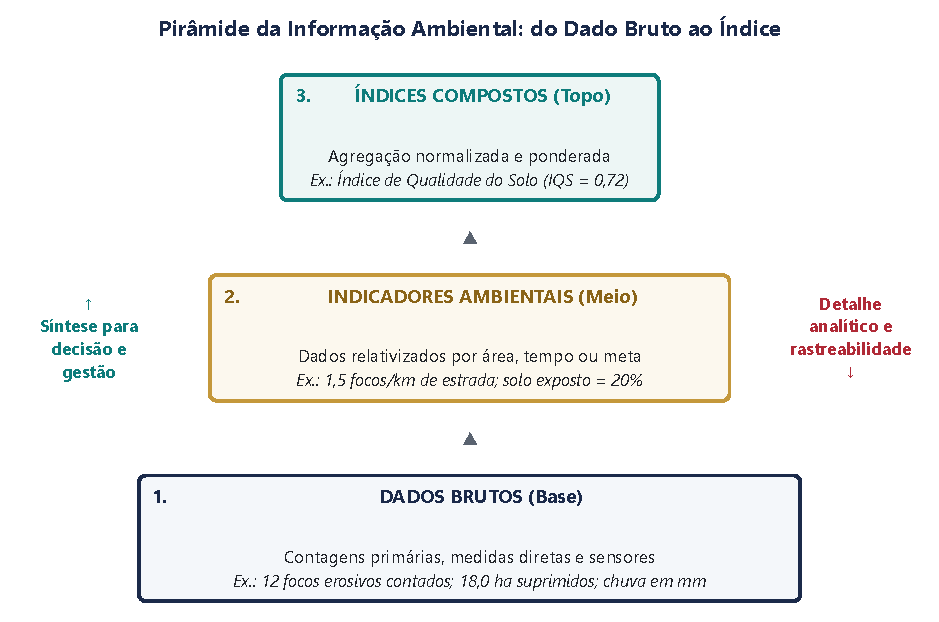
\includegraphics[width=0.90\textwidth]{figures/fig_cap10_piramide_informacao.pdf}
  \caption{Pirâmide da informação ambiental, ilustrando a passagem do dado bruto coletado em campo ao indicador relativizado e ao índice composto de decisão.}
  \label{fig:piramide_informacao}
\end{figure}

\section{Critérios de Seleção de Indicadores Ambientais}

Para evitar a escolha arbitrária de variáveis caras ou pouco informativas, OECD (2003), Fidalgo (2003) e IBGE (2018) consolidam quatro critérios de seleção que todo indicador deve atender antes de ingressar em um programa de monitoramento (Figura~\ref{fig:criterios_ocde}). A \textbf{relevância política e técnica} assegura vínculo direto com um problema concreto ou condicionante legal; a \textbf{solidez analítica} exige base científica reconhecida e protocolo repetível por técnicos independentes; a \textbf{mensurabilidade} verifica viabilidade orçamentária e regularidade temporal da série histórica; e a \textbf{sensibilidade} avalia se o indicador acusa degradação precoce e responde às intervenções corretivas em prazo útil à gestão.

\begin{figure}[H]
  \centering
  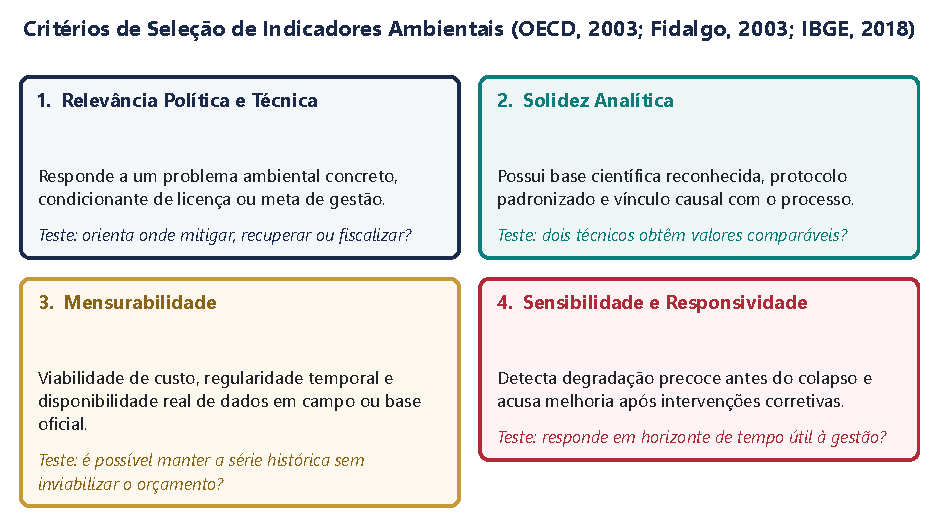
\includegraphics[width=0.92\textwidth]{figures/fig_cap10_criterios_ocde.pdf}
  \caption{Os quatro critérios de seleção de indicadores ambientais (OECD, 2003; Fidalgo, 2003; IBGE, 2018) e suas perguntas de auditoria em campo.}
  \label{fig:criterios_ocde}
\end{figure}

O Exemplo 10.1 aplica esses quatro critérios à triagem de propostas reais em um complexo eólico na Caatinga baiana.

\begin{boxExemplo}{10.1 (Básico)}{Triagem de Indicadores Ambientais segundo os Critérios da OCDE}
\passoEnunciado{Uma equipe técnica da UEFS foi convidada a propor indicadores para monitorar a conservação da Caatinga no entorno de um complexo eólico em Canudos (BA), avaliando quatro candidatos: percentual de área com solo exposto em cortes e platôs (I); percepção genérica de beleza da paisagem sem questionário padronizado (II); densidade de focos erosivos ativos por quilômetro de acesso (III); e sequenciamento genômico semanal de todos os micro-organismos do solo em 80 pontos (IV).}
\passoDados{Critérios obrigatórios de triagem (OECD, 2003; Fidalgo, 2003; IBGE, 2018): relevância política/técnica, solidez analítica, mensurabilidade e sensibilidade, avaliados como \textit{Atende (A)}, \textit{Atende parcialmente (P)} ou \textit{Não atende (N)}.}
\passoPedido{Avaliar os quatro candidatos, justificar quais devem ser selecionados e apontar o critério violado nos indicadores descartados.}
\passoMetodo{Aplicação da matriz de aderência aos quatro critérios de seleção de indicadores ambientais, verificando rigor científico, viabilidade operacional e vínculo direto com o problema de degradação.}
\passoContas{
Os \textbf{Candidatos I e III} atendem plenamente aos quatro critérios: medem proteção superficial e erosão linear com protocolo replicável em campo/imagens (A), baixo custo de repetição semestral (A) e alta sensibilidade a obras de drenagem e revegetação (A). O \textbf{Candidato II} falha em \textbf{solidez analítica (N)} e \textbf{mensurabilidade replicável (N)} por carecer de questionário estruturado e desenho amostral. O \textbf{Candidato IV} falha em \textbf{mensurabilidade operacional e financeira (N)}, com custo proibitivo e ausência de vínculo direto com a gestão de erosão.}
\passoResposta{Selecionam-se os indicadores I e III. O indicador II exige reformulação metodológica; o indicador IV é inviável para o monitoramento rotineiro proposto.}
\passoVerificacao{Os dois indicadores aprovados cobrem diretamente o estado físico da superfície e o impacto erosivo linear com orçamento realista e auditável.}
\end{boxExemplo}

\section{Modelos PER, PEIR e DPSIR: Arquitetura Causal e Construção de Matrizes}

Um conjunto de indicadores ganha força interpretativa quando organizado dentro de uma estrutura lógica que explicite causa, alteração do meio, dano e solução. O modelo \textbf{PER (Pressão--Estado--Resposta)}, formulado por Anthony Friend e David Rapport e difundido pela OCDE (OECD, 2003), parte de uma lógica de retroalimentação na qual atividades humanas exercem \textit{pressões} sobre o meio, modificam o \textit{estado} dos recursos naturais e provocam \textit{respostas} técnicas ou políticas da sociedade voltadas a conter as pressões ou recuperar o ambiente.

Posteriormente, o Programa das Nações Unidas para o Meio Ambiente (PNUMA/UNEP) refinou essa estrutura para o modelo \textbf{PEIR (Pressão--Estado--Impacto--Resposta)}, amplamente adotado pelo IBGE, MMA e órgãos estaduais brasileiros. A inclusão do compartimento \textbf{Impacto (I)} separa com nitidez a alteração biofísica do meio (\textit{Estado}) de suas consequências ecológicas, produtivas e socioambientais (\textit{Impacto}), facilitando a articulação direta com a Avaliação de Impacto Ambiental (Capítulo 5). Em estudos regionais de maior escala, o modelo \textbf{DPSIR} acrescenta ainda a categoria \textbf{Força Motriz (D)} antes da Pressão para explicitar vetores estruturais como metas nacionais de transição energética ou expansão agropecuária (Figura~\ref{fig:modelo_peir_semiarido}).

\begin{figure}[H]
  \centering
  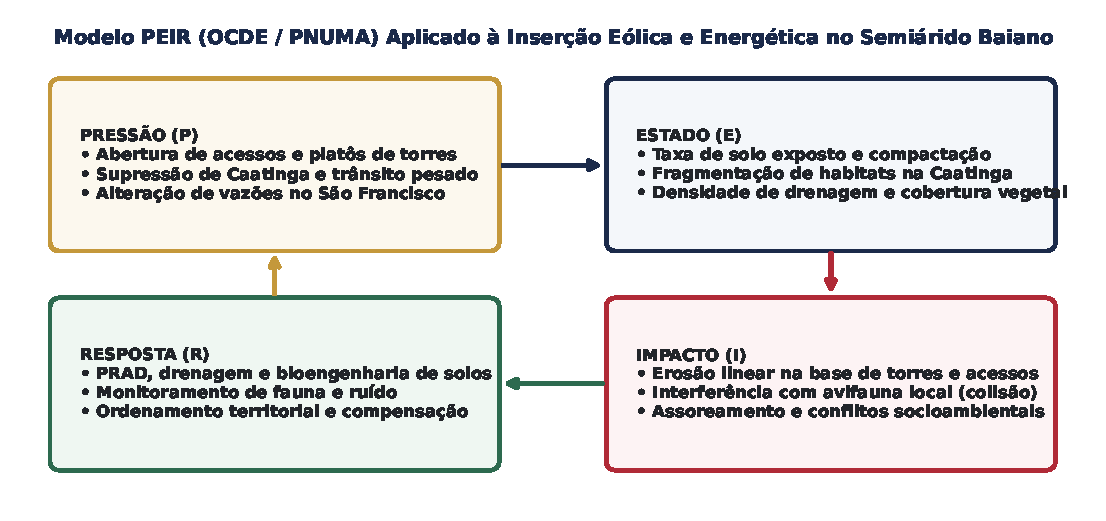
\includegraphics[width=0.94\textwidth]{figures/fig08_modelo_peir_semiarido.pdf}
  \caption{Arquitetura cíclica do modelo PEIR aplicada à inserção eólica e energética no Semiárido Baiano, integrando vetores de pressão, alterações de estado biofísico, impactos socioambientais e respostas de gestão e bioengenharia.}
  \label{fig:modelo_peir_semiarido}
\end{figure}

A leitura da Figura~\ref{fig:modelo_peir_semiarido} evidencia que o modelo PEIR opera como um \textbf{ciclo dinâmico de retroalimentação}. A \textbf{Pressão (P)} reúne ações humanas perturbadoras como a abertura de acessos e platôs ou a operação de barramentos. O \textbf{Estado (E)} retrata a condição observável dos compartimentos, como percentual de solo exposto, compactação e nível dos reservatórios. O \textbf{Impacto (I)} traduz as consequências resultantes sobre ecossistemas e comunidades, incluindo sulcos e ravinas em taludes, colisão de avifauna, assoreamento e conflitos por usos múltiplos da água. A \textbf{Resposta (R)} articula medidas corretivas e de gestão (drenagem controlada, PRAD, bioengenharia e alocação negociada em comitês de bacia), separando indicadores de execução (metros de canaleta construídos) de indicadores de resultado (redução efetiva de focos erosivos).

O Exemplo 10.3 mostra como preencher uma matriz PEIR comparando complexos eólicos e hidrelétricas ao longo do Submédio São Francisco.

\begin{boxExemplo}{10.3 (Intermediário)}{Construção de Matriz PEIR para o Eixo Energético do Submédio São Francisco}
\passoEnunciado{A partir das observações da viagem de campo entre Sobradinho, Casa Nova, Juazeiro, Rodelas e Paulo Afonso, estruture uma matriz PEIR integrando complexos eólicos em bordas de chapada e regularização hidrelétrica de vazões no Rio São Francisco.}
\passoDados{Roteiro de campo DCHF/UEFS e evidências registradas em reservatórios, calha fluvial e parques eólicos instalados sobre Caatinga hiperxerófila.}
\passoPedido{Preencher uma matriz PEIR coerente contendo Pressão, Estado, Impacto e Resposta com indicadores mensuráveis para cada vetor.}
\passoMetodo{Separação rigorosa entre atividade antrópica (P), alteração física ou biótica do compartimento (E), consequência socioambiental (I) e instrumento de gestão ou mitigação (R).}
\passoContas{
\begin{center}
\renewcommand{\arraystretch}{1.2}
\footnotesize
\begin{tabularx}{\textwidth}{@{}p{2.2cm} >{\raggedright\arraybackslash}X >{\raggedright\arraybackslash}X >{\raggedright\arraybackslash}X >{\raggedright\arraybackslash}X@{}}
  \toprule
  \rowcolor{uefsNavy}
  \textcolor{white}{\bfseries Vetor} & \textcolor{white}{\bfseries Pressão (P)} & \textcolor{white}{\bfseries Estado (E)} & \textcolor{white}{\bfseries Impacto (I)} & \textcolor{white}{\bfseries Resposta (R)} \\
  \midrule
  \textbf{Eólicas na Caatinga} & Abertura de acessos e platôs ($\text{ha}$ suprimidos; $D_v$ em $\text{km}\cdot\text{km}^{-2}$). & Solo exposto ($\%$), compactação ($D_s$) e fragmentação vegetal. & Erosão na base de torres (focos/km) e colisão de avifauna (aves/torre/ano). & Drenagem pluvial, PRAD/bioengenharia e zonas de exclusão para rotas de aves. \\
  \rowcolor{bgGray}
  \textbf{Hidrelétricas (São Francisco)} & Operação de reservatórios com redução de vazão defluente ($\text{m}^3\cdot\text{s}^{-1}$). & Alteração do pulso hidrológico, redução de lâmina d'água e bancos arenosos. & Perda de agricultura de vazante, conflitos com irrigação e degradação ripária. & Alocação negociada no CBHSF, vazão ecológica mínima e recomposição de APPs. \\
  \bottomrule
\end{tabularx}
\end{center}}
\passoResposta{A matriz PEIR articulada permite acompanhar separadamente as causas (P), as mudanças mensuráveis do meio (E), os danos ecológicos e sociais (I) e a efetividade das ações corretivas (R) nos dois eixos energéticos.}
\passoVerificacao{Cada coluna apresenta grandezas verificáveis e evita classificar uma atividade (pressão) como impacto ou um programa de monitoramento (resposta) como estado ambiental.}
\end{boxExemplo}

Ao montar uma matriz PEIR pela primeira vez, um equívoco recorrente consiste em misturar a ação humana causadora com a consequência física resultante, conforme destacado no alerta a seguir.

\begin{boxErro}[Erro 1: Confundir Dado Bruto, Pressão e Impacto na Matriz PEIR]
\textbf{Equívoco frequente:} Listar ``abertura de $18\text{ km}$ de estradas'' na coluna de Impacto (I) ou registrar ``execução de PRAD'' na coluna de Estado (E).\par
\textbf{Correção técnica:} A abertura de estradas é a ação humana geradora de perturbação, logo pertence à \textbf{Pressão (P)}. A execução do PRAD é uma intervenção corretiva da sociedade, portanto é \textbf{Resposta (R)}. O \textbf{Estado (E)} retrata a condição biofísica resultante (percentual de solo exposto), enquanto o \textbf{Impacto (I)} expressa o dano ou consequência (ravinamento em taludes, perda de biodiversidade, assoreamento).
\end{boxErro}

\section{Métricas Operacionais de Campo e Ficha do Indicador}

Para transformar observações de campo em indicadores auditáveis na matriz PEIR, empregam-se relações quantitativas com unidades explícitas acompanhadas de uma \textbf{ficha técnica padronizada}. Cada indicador deve registrar obrigatoriamente fonte dos dados, unidade de medida, período ou frequência de coleta, método de levantamento e área de referência, assegurando reprodutibilidade científica e comparação válida entre campanhas ao longo do tempo e entre setores distintos. Na ficha de cada indicador, um trecho sem vistoria constitui informação ausente, jamais valor zero, pois atribuir zero onde não houve inspeção derruba artificialmente a média calculada e mascara focos críticos de degradação.

\begin{boxFormula}[Métricas Operacionais de Campo e Monitoramento (Modelo PEIR)]
\begin{align}
  T_{\text{sup}} &= \frac{A_{\text{sup}}}{A_{\text{pol}}} \times 100\% \qquad \text{(Taxa de supressão vegetal, em \%)} \\[5pt]
  D_v &= \frac{L_{\text{acessos}}}{A_{\text{km}^2}} \qquad \text{(Densidade viária de serviço, em km}\cdot\text{km}^{-2}\text{)} \\[5pt]
  M_{\text{est}} &= \frac{N_{\text{obs}}}{e \cdot p} \qquad \text{(Mortalidade corrigida de avifauna, em aves}\cdot\text{ano}^{-1}\text{)} \\[5pt]
  \Delta_{\%} &= \frac{X_{\text{final}} - X_{\text{inicial}}}{X_{\text{inicial}}} \times 100\% \qquad \text{(Variação percentual de estado ou resposta)}
\end{align}
Nessas expressões, $A_{\text{sup}}$ é a área suprimida ($\text{ha}$) e $A_{\text{pol}}$ é a área total da poligonal ($\text{ha}$, lembrando que $1\text{ km}^2 = 100\text{ ha}$). A variável $A_{\text{km}^2}$ representa a área da poligonal em $\text{km}^2$ e $L_{\text{acessos}}$ indica a extensão total de estradas internas ($\text{km}$). Na estimativa faunística, $N_{\text{obs}}$ corresponde às carcaças encontradas em $1\text{ ano}$, $e \in (0, 1]$ expressa a eficiência do observador na busca e $p \in (0, 1]$ representa a probabilidade de a carcaça persistir no terreno sem remoção por necrófagos entre vistorias. Por fim, $\Delta_{\%}$ mede a variação relativa entre os valores inicial e final, devendo ser distinguida da variação em \textbf{pontos percentuais} (diferença direta entre taxas já expressas em porcentagem).
\end{boxFormula}

O Exemplo 10.2 demonstra o cálculo conjunto da taxa de supressão e da densidade viária em um parque eólico no Semiárido.

\begin{boxExemplo}{10.2 (Intermediário)}{Cálculo de Supressão Vegetal e Densidade Viária em Parque Eólico}
\passoEnunciado{Durante a análise do Estudo de Impacto Ambiental (EIA) de um parque eólico situado em uma chapada no eixo Canudos--Sento Sé, quantifique a taxa percentual de supressão da Caatinga e a densidade de acessos internos dentro da poligonal do empreendimento.}
\passoDados{Área total da poligonal: $A_{\text{pol}} = 1.600\text{ ha}$. Aerogeradores: $25$ torres com platô de $0{,}45\text{ ha}$ cada. Estradas internas: $L_{\text{acessos}} = 18{,}0\text{ km}$ com largura média de $10\text{ m}$. Subestação e canteiro: $2{,}75\text{ ha}$.}
\passoPedido{Calcular a área total suprimida $A_{\text{sup}}$ em hectares, a taxa percentual de supressão $T_{\text{sup}}$ e a densidade viária interna $D_v$ em $\text{km}\cdot\text{km}^{-2}$.}
\passoMetodo{Conversão homogênea de unidades métricas para hectares ($1\text{ ha} = 10.000\text{ m}^2$) e quilômetros quadrados ($1\text{ km}^2 = 100\text{ ha}$).}
\passoContas{
\textbf{Etapa 1, Área dos platôs e das estradas de acesso ($18{,}0\text{ km} = 18.000\text{ m}$):}
\[
A_{\text{platôs}} = 25 \times 0{,}45\text{ ha} = 11{,}25\text{ ha} \qquad\qquad A_{\text{acessos}} = \frac{18.000\text{ m} \times 10\text{ m}}{10.000\text{ m}^2\cdot\text{ha}^{-1}} = 18{,}00\text{ ha}
\]
\textbf{Etapa 2, Área total suprimida, taxa percentual e densidade viária ($A_{\text{km}^2} = 1.600 / 100 = 16{,}0\text{ km}^2$):}
\begin{align*}
A_{\text{sup}} &= 11{,}25 + 18{,}00 + 2{,}75 = 32{,}00\text{ ha} \\
T_{\text{sup}} &= \frac{32{,}00}{1.600} \times 100\% = 2{,}00\% \qquad D_v = \frac{18{,}0\text{ km}}{16{,}0\text{ km}^2} = 1{,}125\text{ km}\cdot\text{km}^{-2}
\end{align*}}
\passoResposta{Área total suprimida de $32{,}00\text{ ha}$, taxa de supressão de $2{,}00\%$ da poligonal e densidade viária interna de $1{,}125\text{ km}\cdot\text{km}^{-2}$.}
\passoVerificacao{Embora $2{,}00\%$ pareça um percentual reduzido em área absoluta, $56{,}25\%$ do total suprimido ($18{,}0\text{ ha}$) corresponde a corredores lineares, gerando densidade viária superior a $1\text{ km}\cdot\text{km}^{-2}$ e potencializando a fragmentação da Caatinga.}
\end{boxExemplo}

A interpretação isolada de $T_{\text{sup}}$ sem o cruzamento com $D_v$ leva frequentemente à subestimação dos impactos lineares sobre a fauna e a drenagem, conforme alertado a seguir.

\begin{boxErro}[Erro 2: Subestimar a Fragmentação ao Olhar Apenas o Percentual Total de Supressão]
\textbf{Equívoco frequente:} Concluir que uma taxa de supressão de $2\%$ em um parque eólico é ecologicamente irrelevante.\par
\textbf{Correção técnica:} Um pequeno percentual distribuído em malha viária extensa e linhas de transmissão cria centenas de metros de borda exposta, interrompe o deslocamento de fauna terrestre e concentra o escoamento superficial das chuvas torrenciais do Semiárido. Por isso, complementa-se $T_{\text{sup}}$ com métricas espaciais como a densidade viária ($D_v$).
\end{boxErro}

No monitoramento da avifauna, contar apenas carcaças visíveis subestima a mortalidade real porque parte delas passa despercebida na vegetação ($e < 1$) ou é removida por necrófagos antes da vistoria ($p < 1$). A comparação entre taxa bruta e corrigida contra o limiar de alerta, bem como a resposta quantitativa das medidas corretivas em um PRAD, pode ser visualizada diretamente na Figura~\ref{fig:mortalidade_eficacia} e detalhada no Exemplo 10.4.

\begin{figure}[H]
  \centering
  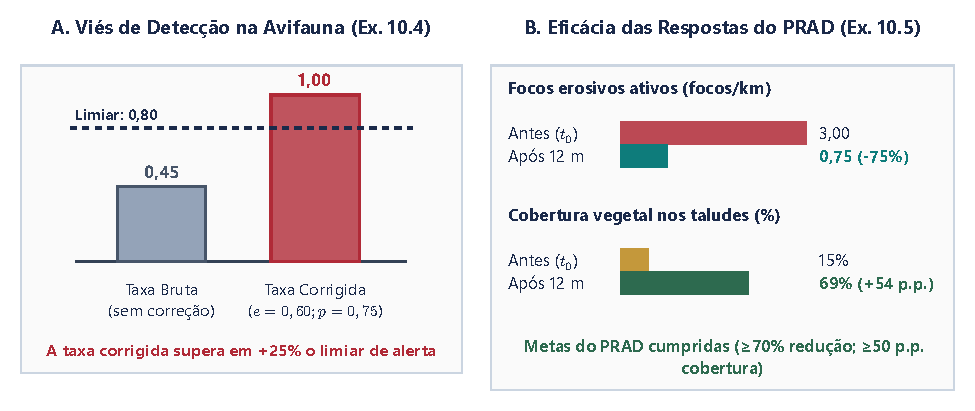
\includegraphics[width=0.92\textwidth]{figures/fig_cap10_mortalidade_eficacia.pdf}
  \caption{Comparação visual entre taxa bruta e corrigida na estimativa de mortalidade de avifauna frente ao limiar de alerta (A) e resposta quantitativa dos indicadores de recuperação após execução de PRAD (B).}
  \label{fig:mortalidade_eficacia}
\end{figure}

\begin{boxExemplo}{10.4 (Avançado)}{Indicador Corrigido de Mortalidade de Avifauna em Parque Eólico}
\passoEnunciado{O monitoramento de avifauna em um parque eólico com $40$ aerogeradores próximo a corredores ecológicos da Caatinga baiana registrou, em 12 meses de vistorias padronizadas, $18$ carcaças de aves associadas à colisão. Testes de campo indicaram eficiência de busca $e = 0{,}60$ e persistência de carcaças $p = 0{,}75$.}
\passoDados{$N_{\text{obs}} = 18$ aves/ano; $N_t = 40$ torres; $e = 0{,}60$; $p = 0{,}75$. Limiar operacional de alerta: $0{,}80\text{ ave}\cdot\text{torre}^{-1}\cdot\text{ano}^{-1}$.}
\passoPedido{Calcular a taxa bruta não corrigida por torre, a mortalidade anual estimada corrigida $M_{\text{est}}$ e a taxa corrigida por torre/ano, comparando-a ao limiar de alerta.}
\passoMetodo{Aplicação do fator de correção amostral $M_{\text{est}} = N_{\text{obs}} / (e \cdot p)$ e relativização pelo número de aerogeradores.}
\passoContas{
\begin{align*}
T_{\text{bruta}} &= \frac{18}{40} = 0{,}45\text{ ave}\cdot\text{torre}^{-1}\cdot\text{ano}^{-1} \\
e \cdot p &= 0{,}60 \times 0{,}75 = 0{,}45 \quad (\text{apenas } 45\% \text{ de detecção})
\end{align*}
\begin{align*}
M_{\text{est}} &= \frac{18}{0{,}45} = 40{,}0\text{ aves}\cdot\text{ano}^{-1} \\
T_{\text{corr}} &= \frac{40{,}0}{40} = 1{,}00\text{ ave}\cdot\text{torre}^{-1}\cdot\text{ano}^{-1}
\end{align*}
Como $1{,}00 > 0{,}80$, o limiar de alerta foi ultrapassado em $25\%$ ($\frac{1{,}00 - 0{,}80}{0{,}80}\times 100\%$).}
\passoResposta{Taxa bruta de $0{,}45\text{ ave}\cdot\text{torre}^{-1}\cdot\text{ano}^{-1}$, mas taxa corrigida de $1{,}00\text{ ave}\cdot\text{torre}^{-1}\cdot\text{ano}^{-1}$ ($M_{\text{est}} = 40$ aves/ano), superando o limiar de alerta e exigindo resposta mitigadora imediata.}
\passoVerificacao{Conforme ilustrado no Painel A da Figura~\ref{fig:mortalidade_eficacia}, a taxa bruta ocultaria a ultrapassagem do limiar caso os fatores de detecção e persistência fossem omitidos.}
\end{boxExemplo}

Sem padronização do esforço amostral e correção do viés de detecção, comparações entre campanhas perdem validade técnica.

\begin{boxErro}[Erro 3: Comparar Contagens Brutas de Fauna ou Erosão sem Padronização Amostral]
\textbf{Equívoco frequente:} Relatar apenas o número absoluto de carcaças de aves ou focos erosivos sem considerar esforço amostral, número de torres, extensão vistoriada ou eficiência de detecção.\par
\textbf{Correção técnica:} Sem relativização (por torre/ano ou por $\text{km}$ de estrada) e sem correção de viés de detecção ($e \cdot p$ no monitoramento faunístico), os números não são comparáveis entre campanhas nem entre empreendimentos, comprometendo a solidez analítica exigida pela OCDE (2003).
\end{boxErro}

\section{Estudo de Caso Integrado: Viagem de Campo no Semiárido Baiano}

A atividade de campo prevista na Semana 11 do Plano CHF662 percorre a região de \textbf{Canudos} e o eixo energético do \textbf{Submédio São Francisco}, nos municípios de \textbf{Paulo Afonso, Rodelas, Sobradinho, Casa Nova, Sento Sé e Juazeiro}, onde coexistem o bioma \textbf{Caatinga}, chapadas e serras residuais, o maior eixo hidrelétrico do Nordeste e grandes complexos eólicos e fotovoltaicos.

\subsection{Fatores Locacionais e Leitura das Infraestruturas em Campo}

A concentração de parques eólicos resulta da convergência entre o \textbf{regime de ventos alísios de sudeste e leste} (velocidades médias frequentemente entre $7{,}5$ e $9{,}5\text{ m}\cdot\text{s}^{-1}$ a $100\text{ m}$, com máxima intensidade no segundo semestre seco e complementaridade sazonal à geração hidrelétrica), o \textbf{relevo de chapadas e serras residuais} que acelera o escoamento por efeito topográfico, a \textbf{proximidade de linhas de transmissão do SIN} estruturadas a partir de Paulo Afonso e Sobradinho, e a \textbf{estrutura fundiária} com grandes imóveis e áreas de fundo de pasto.

Em campo, observa-se como os acessos e plataformas dos aerogeradores conectam a implantação elétrica à dinâmica da vertente (Figura~\ref{fig:canudos_acessos}). Superfícies expostas recebem o impacto direto das gotas de chuva, enquanto valetas e bueiros redirecionam o escoamento superficial concentrado.

\begin{figure}[H]
  \centering
  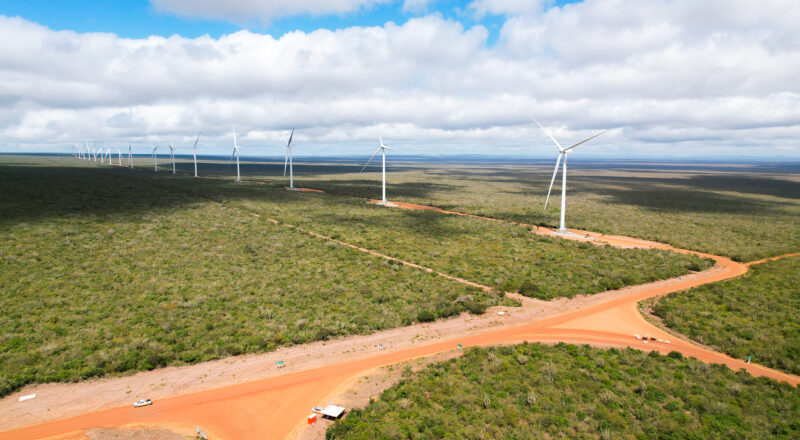
\includegraphics[width=0.78\textwidth]{figures/eolica_canudos_1.jpg}
  \caption{Aerogeradores, plataformas e acessos em área de Caatinga no eixo de Canudos. Fonte: acervo didático da disciplina.}
  \label{fig:canudos_acessos}
\end{figure}

Quando o arranjo linear das estradas de serviço atravessa divisores e unidades de drenagem, a continuidade dos corredores de solo exposto amplia a fragmentação da Caatinga e aproxima a enxurrada dos canais intermitentes (Figura~\ref{fig:canudos_linear}).

\begin{figure}[H]
  \centering
  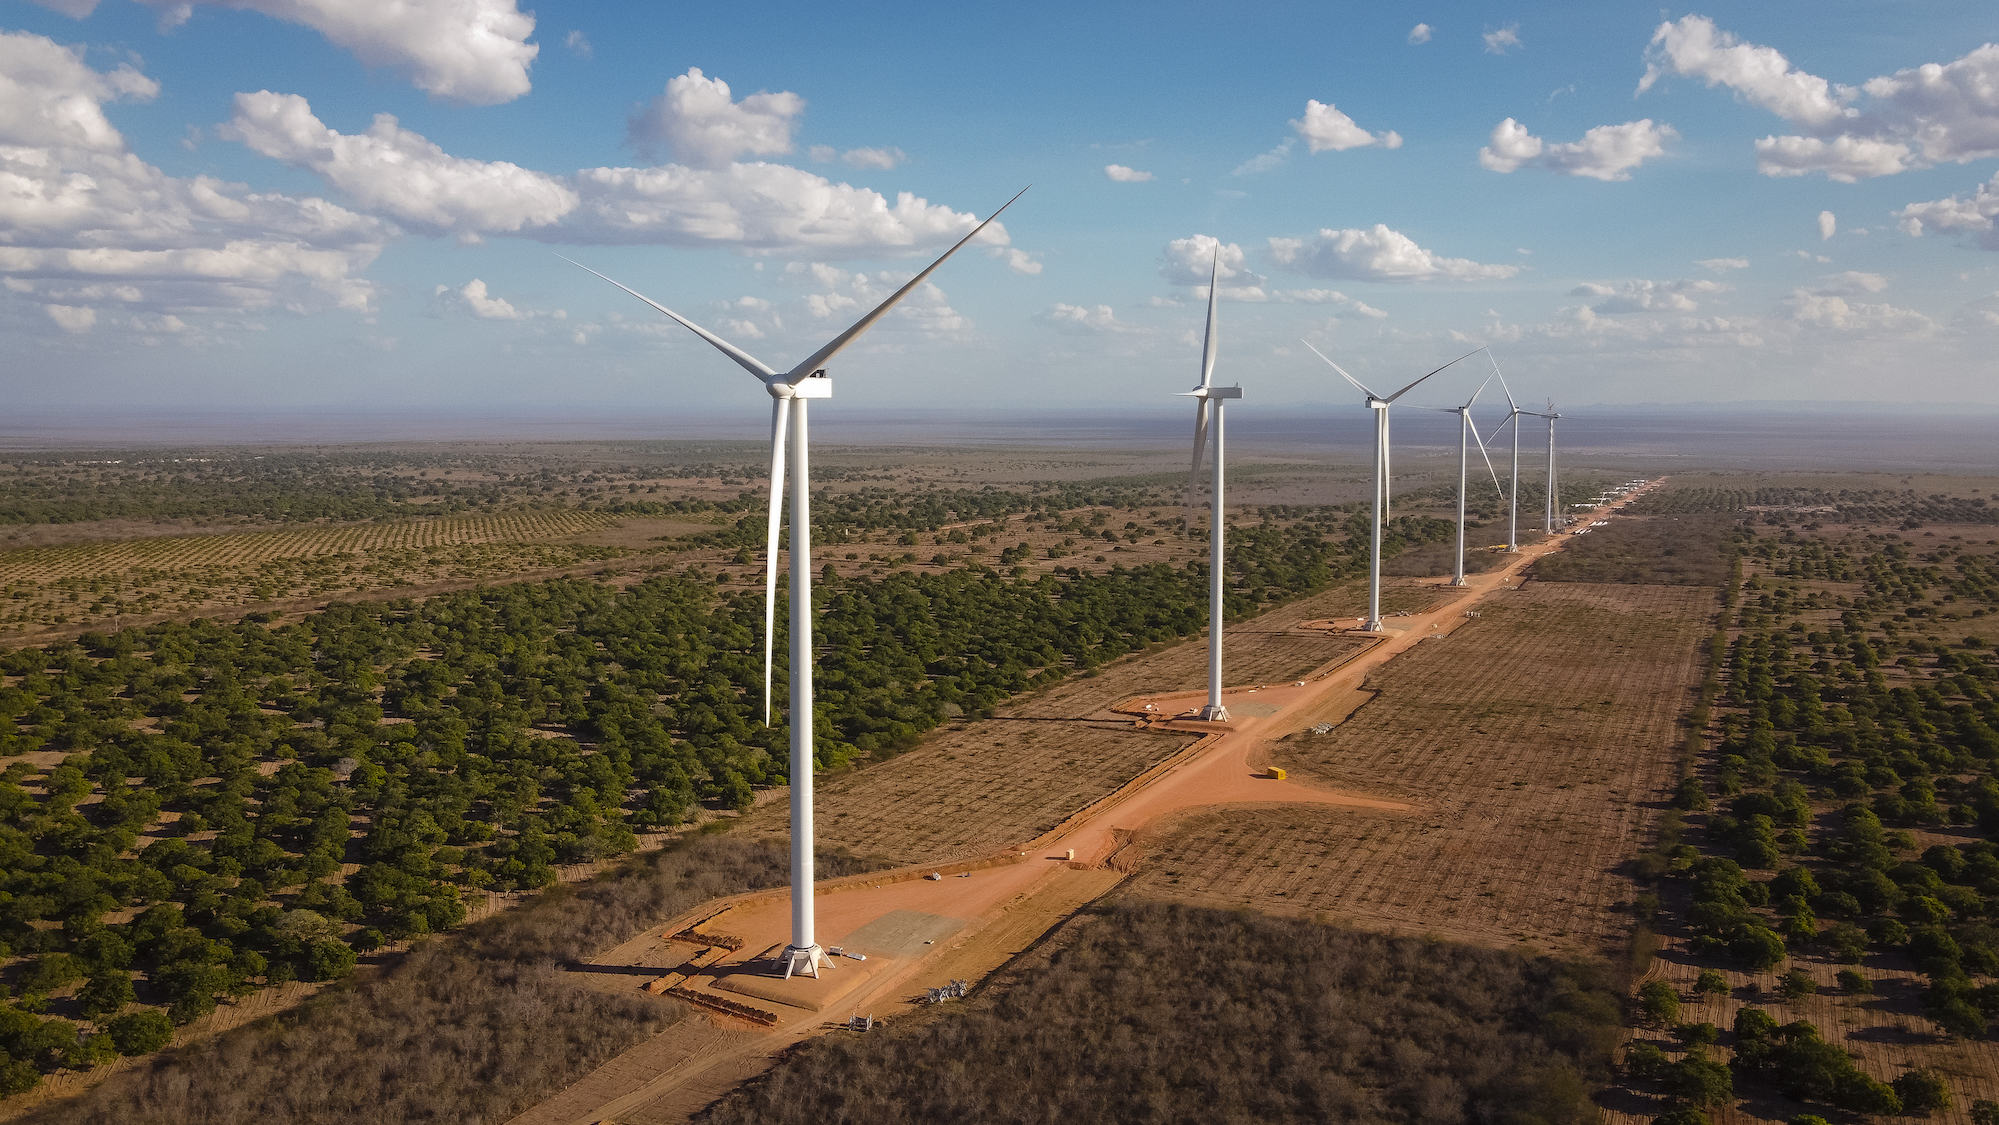
\includegraphics[width=0.78\textwidth]{figures/eolica_canudos_2.jpg}
  \caption{Arranjo linear de aerogeradores e acessos de serviço sobre superfície de solo exposto em Canudos. Fonte: acervo didático da disciplina.}
  \label{fig:canudos_linear}
\end{figure}

No eixo fluvial do Submédio São Francisco, o armazenamento hidrelétrico em Sobradinho modifica o pulso natural de cheias e vazantes, conectando geração elétrica, irrigação, abastecimento e pesca artesanal (Figura~\ref{fig:sobradinho_usina}).

\begin{figure}[H]
  \centering
  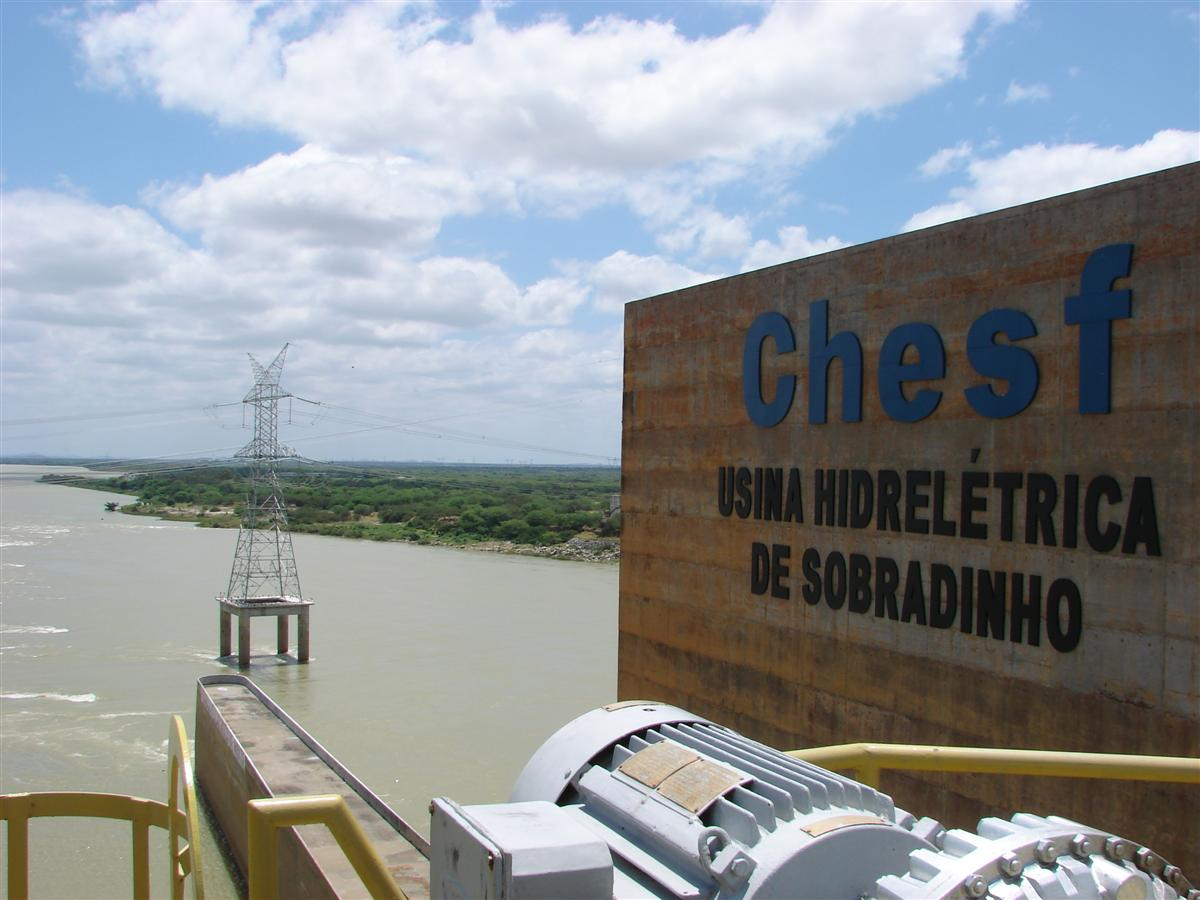
\includegraphics[width=0.78\textwidth]{figures/sobradinho_usina_glauco_umbelino.jpg}
  \caption{Usina Hidrelétrica de Sobradinho, Bahia. Fotografia de Glauco Umbelino (Wikimedia Commons, CC BY 2.0).}
  \label{fig:sobradinho_usina}
\end{figure}

Em reservatórios e chapadas semiáridas, arranjos fotovoltaicos acrescentam novas interfaces territoriais associadas à supressão vegetal em áreas planas ou à cobertura parcial do espelho d'água em sistemas flutuantes (Figura~\ref{fig:sento_se_solar}).

\begin{figure}[H]
  \centering
  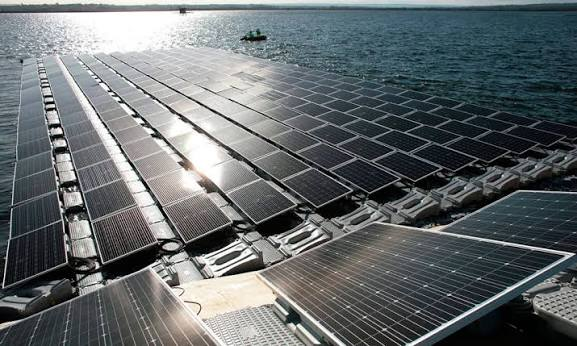
\includegraphics[width=0.78\textwidth]{figures/sento_se_solar_1.jpg}
  \caption{Módulos fotovoltaicos instalados em sistema flutuante sobre reservatório. Fonte: acervo didático da disciplina.}
  \label{fig:sento_se_solar}
\end{figure}

\subsection{Convivência com a Caatinga, Roteiro e Principais Impactos Ambientais}

A avaliação de campo no eixo Canudos--Submédio São Francisco evidencia impactos concentrados na fase de implantação e na reorganização territorial, entre os quais se destacam a supressão e a fragmentação da Caatinga por platôs e acessos para pás de $60$ a $80\text{ m}$, a erosão na base das torres e cortes de estrada em solos rasos sob chuvas convectivas concentradas, além das disputas por usos múltiplos da água diante da regularização de vazões no Rio São Francisco.

No componente faunístico, a implantação de aerogeradores e linhas de transmissão em corredores aéreos eleva o risco de colisão e cria efeito barreira para a arara-azul-de-lear (\textit{Anodorhynchus leari}), espécie endêmica e ameaçada que realiza deslocamentos diários entre os paredões areníticos usados como dormitórios e ninheiras no Raso da Catarina e as áreas de alimentação com licurizeiros (\textit{Syagrus coronata}) no entorno de Canudos (Figura~\ref{fig:arara_azul_lear}). O monitoramento contínuo das rotas de voo e o ajuste locacional de torres constituem condicionantes centrais para conciliar a geração renovável com a conservação da Caatinga.

\begin{figure}[H]
  \centering
  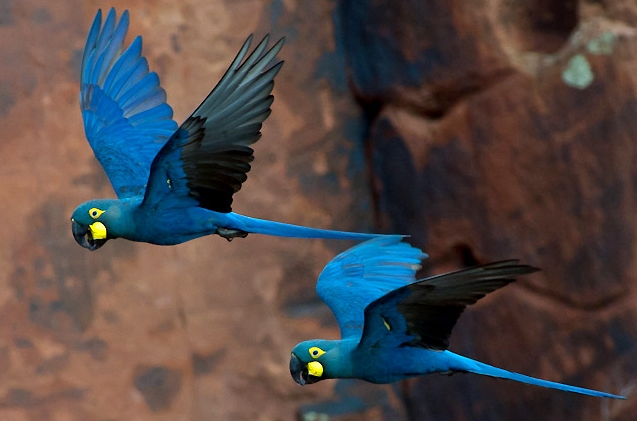
\includegraphics[width=0.76\textwidth]{figures/anodorhynchus_lear.jpg}
  \caption{Exemplares de arara-azul-de-lear (\textit{Anodorhynchus leari}) em voo junto aos paredões areníticos do Raso da Catarina, Canudos (BA), área crítica para dormitórios e corredores de forrageamento na Caatinga. Fonte: acervo didático da disciplina.}
  \label{fig:arara_azul_lear}
\end{figure}

Durante o roteiro prático, a equipe discente registra evidências georreferenciadas integrando quatro eixos: relevo e substrato (posição das torres, solos rasos e declividade), processos erosivos e drenagem (selamento, sulcos e saídas pluviais), cobertura da Caatinga e fauna (fisionomia vegetal, licurizeiros e efeito de borda) e dinâmica hídrica e socioambiental (nível dos reservatórios, irrigação e comunidades de fundo de pasto).

\etapa{4}{Avaliação de Eficácia de Respostas no Ciclo PEIR}

No fechamento do ciclo PEIR, o monitoramento pós-obra verifica quantitativamente se as ações de drenagem e revegetação cumpriram as metas estabelecidas no PRAD, como representado no Painel B da Figura~\ref{fig:mortalidade_eficacia} e calculado no Exemplo 10.5.

\begin{boxExemplo}{10.5 (Avançado)}{Avaliação Quantitativa de Eficácia de Resposta Mitigadora no Ciclo PEIR}
\passoEnunciado{Após vistoria de campo apontar erosão acelerada nos acessos de um complexo eólico no Semiárido, o empreendedor executou um programa de resposta (R) combinando canaletas revestidas, dissipadores em pedra rachão, paliçadas permeáveis e semeadura de espécies nativas da Caatinga nos taludes. Antes das obras, havia $36$ focos erosivos ativos ao longo de $12\text{ km}$ de estradas e cobertura vegetal média nos taludes de $15\%$. Doze meses após as intervenções, nova vistoria registrou $9$ focos ativos e cobertura vegetal média de $69\%$.}
\passoDados{Antes: $F_0 = 36$ focos em $12\text{ km}$; cobertura $C_0 = 15\%$. Depois (12 meses): $F_1 = 9$ focos em $12\text{ km}$; cobertura $C_1 = 69\%$. Meta contratual do PRAD: redução mínima de $70\%$ nos focos erosivos e incremento mínimo de $50$ pontos percentuais na cobertura vegetal.}
\passoPedido{Calcular a densidade inicial e final de focos erosivos, a redução percentual dos focos e o ganho absoluto (pontos percentuais) e relativo na cobertura vegetal, verificando o cumprimento das metas.}
\passoMetodo{Cálculo das razões por quilômetro de acesso e das variações absoluta e percentual entre os tempos $t_0$ e $t_1$.}
\passoContas{
\begin{align*}
D_{f,0} &= \frac{36}{12} = 3{,}00\text{ focos}\cdot\text{km}^{-1} \qquad & D_{f,1} &= \frac{9}{12} = 0{,}75\text{ foco}\cdot\text{km}^{-1} \\
\Delta F_{\%} &= \frac{9 - 36}{36} \times 100\% = -75{,}0\% & \Delta C_{\text{pp}} &= 69\% - 15\% = +54\text{ p.p.} \\
\Delta C_{\text{rel}} &= \frac{69 - 15}{15} \times 100\% = +360{,}0\% & &
\end{align*}
Conferência frente às metas: $75{,}0\% \ge 70\%$ (cumprida) e $54\text{ p.p.} \ge 50\text{ p.p.}$ (cumprida).}
\passoResposta{A densidade de focos caiu de $3{,}00$ para $0{,}75\text{ foco}\cdot\text{km}^{-1}$ (redução de $75{,}0\%$) e a cobertura vegetal avançou $+54$ pontos percentuais ($+360{,}0\%$ relativos), cumprindo ambas as metas do PRAD.}
\passoVerificacao{Distinguir \textit{pontos percentuais} ($69\% - 15\% = 54\text{ p.p.}$) de \textit{variação relativa} ($+360\%$) evita ambiguidades em auditorias ambientais, e os $9$ focos remanescentes indicam necessidade de manutenção pontual.}
\end{boxExemplo}

\etapa{5}{Armadilha Conceitual e Materiais Audiovisuais de Apoio}

Mesmo quando um empreendimento contribui para a descarbonização da matriz elétrica, o diagnóstico territorial continua indispensável para prevenir impactos locais sobre solo, água e fauna.

\begin{boxErro}[Erro 4: Assumir que Energia Eólica Equivale a Impacto Ambiental Nulo]
\textbf{Equívoco frequente:} Afirmar em diagnósticos que parques eólicos na Caatinga não causam degradação por serem fontes renováveis de baixa emissão de carbono.\par
\textbf{Correção técnica:} Toda fonte energética possui pegada territorial. No Semiárido Baiano, a implantação eólica envolve terraplenagem pesada, supressão linear da Caatinga, erosão em solos rasos de chapadas, riscos à avifauna (como a arara-azul-de-lear em Canudos) e conflitos fundiários e sonoros que exigem licenciamento rigoroso e monitoramento contínuo.
\end{boxErro}

Para aprofundar o entendimento sobre indicadores simples, índices compostos e comunicação em relatórios ambientais, assista aos vídeos selecionados na página da disciplina: \textit{Indicadores e relatórios de sustentabilidade} (\url{https://www.youtube.com/watch?v=xk-Y_YivFpU}) e \textit{Você sabe o que é o Índice de Qualidade da Água (IQA)?} (\url{https://www.youtube.com/watch?v=J2HRZjnC03w}), que exemplificam a agregação e interpretação de índices ambientais.

\etapa{6}{Exercícios de Fixação}

\subsection*{Nível Básico (Conceitos, Critérios e Modelo PEIR)}

\begin{enumerate}[leftmargin=1.8em, itemsep=6pt]
  \item Explique, com um exemplo concreto ligado ao Semiárido Baiano, a diferença entre \textbf{dado bruto}, \textbf{indicador ambiental} e \textbf{índice ambiental}.
  \espacoResolucao[1.8cm]

  \item Cite os quatro critérios principais de seleção de indicadores ambientais propostos por OECD (2003), Fidalgo (2003) e IBGE (2018), explicando o risco técnico de ignorar o critério da \textit{mensurabilidade}.
  \espacoResolucao[1.8cm]

  \item Qual é a principal diferença conceitual entre o modelo \textbf{PER} (OCDE) e o modelo \textbf{PEIR} (PNUMA/GEO)? Por que essa distinção favorece a articulação com a Avaliação de Impacto Ambiental?
  \espacoResolucao[1.8cm]

  \item Classifique cada item abaixo como \textbf{Pressão (P)}, \textbf{Estado (E)}, \textbf{Impacto (I)} ou \textbf{Resposta (R)} em um parque eólico na Caatinga: (a) abertura de $14\text{ km}$ de estradas de acesso; (b) ravina ativa de $1{,}8\text{ m}$ de profundidade na saída de bueiro; (c) percentual de solo exposto de $42\%$ no talude; (d) instalação de dissipadores de energia e revegetação com espécies nativas.
  \espacoResolucao[1.8cm]

  \item Liste três fatores locacionais geográficos que explicam a intensa concentração de parques eólicos na região de Canudos e no eixo do Submédio São Francisco (Casa Nova, Sento Sé e entorno de Sobradinho).
  \espacoResolucao[1.8cm]
\end{enumerate}

\subsection*{Nível Intermediário (Cálculos de Monitoramento e Interpretação Regional)}

\begin{enumerate}[leftmargin=1.8em, itemsep=6pt, resume]
  \item Um projeto eólico em uma poligonal de $1.200\text{ ha}$ na Bahia prevê $30$ aerogeradores com platôs de $0{,}40\text{ ha}$ cada, $12\text{ km}$ de acessos internos com $8\text{ m}$ de largura média e $2{,}4\text{ ha}$ destinados à subestação. Calcule a área total suprimida ($A_{\text{sup}}$) e a taxa percentual de supressão ($T_{\text{sup}}$).
  \espacoResolucao[2.2cm]

  \item Em um período de estiagem prolongada no Submédio São Francisco, a vazão defluente média da Usina Hidrelétrica de Sobradinho foi reduzida de $1.300\text{ m}^3\cdot\text{s}^{-1}$ para $800\text{ m}^3\cdot\text{s}^{-1}$. Calcule a variação percentual dessa vazão e cite dois impactos socioambientais diretos dessa redução ao longo do eixo Juazeiro--Rodelas--Paulo Afonso.
  \espacoResolucao[2.2cm]

  \item No monitoramento anual de avifauna de um complexo eólico com $50$ torres, registraram-se $24$ carcaças de aves. Ensaios de campo indicaram eficiência de busca $e = 0{,}80$ e persistência de carcaças $p = 0{,}60$. Calcule a mortalidade total estimada ($M_{\text{est}}$) e a taxa corrigida de mortalidade em aves por torre por ano.
  \espacoResolucao[2.2cm]

  \item Uma poligonal de empreendimento energético abrange $1.500\text{ ha}$ e contém $27\text{ km}$ de estradas internas não pavimentadas. Determine a densidade viária interna ($D_v$) em $\text{km}\cdot\text{km}^{-2}$ e discuta como esse indicador se relaciona com a erosão linear na Caatinga.
  \espacoResolucao[2.0cm]

  \item Após obras de drenagem superficial e bioengenharia nos taludes de um parque eólico, o número de focos erosivos ativos reduziu-se de $28$ para $7$ em um ano. Calcule a redução percentual obtida e classifique esse indicador dentro do modelo PEIR.
  \espacoResolucao[2.0cm]
\end{enumerate}

\subsection*{Nível Aplicado (Questões Objetivas A--E)}

\begin{enumerate}[leftmargin=1.8em, itemsep=6pt, resume]
  \item Sobre os critérios de seleção de indicadores ambientais (OECD, 2003; IBGE, 2018), assinale a alternativa correta:
  \begin{alternativas}
    \item Um indicador de alta qualidade deve dispensar qualquer protocolo padronizado, permitindo interpretações subjetivas de cada analista.
    \item A sensibilidade indica a capacidade do indicador de detectar mudanças ambientais precoces e responder às medidas de manejo em prazo útil.
    \item Indicadores compostos (índices) sempre substituem integralmente os indicadores individuais, tornando desnecessário reportar as variáveis de origem.
    \item A relevância técnica exige que o indicador utilize equipamentos laboratoriais de alto custo, independentemente da viabilidade de monitoramento contínuo.
    \item A mensurabilidade refere-se exclusivamente à possibilidade de converter variáveis qualitativas em médias aritméticas sem base amostral.
  \end{alternativas}

  \item Na matriz PEIR aplicada ao eixo energético do Submédio São Francisco, a ``implantação de um programa de monitoramento telemétrico da arara-azul-de-lear e readequação do traçado de linhas de transmissão'' corresponde ao componente:
  \begin{alternativas}
    \item Pressão (P), pois altera o cronograma financeiro do empreendimento.
    \item Estado (E), pois descreve a abundância natural da espécie na Caatinga.
    \item Impacto (I), pois representa o dano causado pelas torres ao habitat.
    \item Resposta (R), pois consiste em ação técnica e de gestão destinada a prevenir ou mitigar impactos sobre a fauna.
    \item Fator abiótico de base, externo ao ciclo PEIR.
  \end{alternativas}

  \item Um parque eólico localizado em área de $2.000\text{ ha}$ suprimiu $0{,}50\text{ ha}$ por platô em $20$ torres e abriu $15\text{ km}$ de acessos com $10\text{ m}$ de largura. Sem outras áreas suprimidas, a taxa percentual de supressão ($T_{\text{sup}}$) da poligonal é igual a:
  \begin{alternativas}
    \item $0{,}50\%$.
    \item $0{,}75\%$.
    \item $1{,}25\%$.
    \item $2{,}50\%$.
    \item $5{,}00\%$.
  \end{alternativas}

  \item Em relação aos processos físicos observados em parques eólicos implantados em chapadas e serras residuais do Semiárido Baiano, é correto afirmar que:
  \begin{alternativas}
    \item A baixa pluviosidade anual do Semiárido impede completamente a ocorrência de erosão hídrica linear na base das torres.
    \item O terraplenamento de platôs e o escoamento concentrado em estradas compactadas sobre solos rasos potencializam sulcos, ravinas e assoreamento de drenagens intermitentes.
    \item A substituição da Caatinga por solo exposto em taludes de corte reduz a energia cinética do escoamento superficial.
    \item A instalação de aerogeradores elimina a necessidade de medidas de drenagem pluvial e PRAD por se tratar de energia renovável.
    \item Os ventos alísios de sudeste são os únicos responsáveis pelo transporte de sedimentos grosseiros nos bueiros das estradas de acesso.
  \end{alternativas}

  \item Em um programa de monitoramento de colisão de avifauna com $25$ torres eólicas durante um ano, foram encontradas $15$ carcaças. Sabendo que a eficiência de busca foi $e = 0{,}50$ e a persistência de carcaças foi $p = 0{,}60$, a taxa anual corrigida de mortalidade por torre é:
  \begin{alternativas}
    \item $0{,}60\text{ ave}\cdot\text{torre}^{-1}\cdot\text{ano}^{-1}$.
    \item $1{,}20\text{ aves}\cdot\text{torre}^{-1}\cdot\text{ano}^{-1}$.
    \item $1{,}50\text{ aves}\cdot\text{torre}^{-1}\cdot\text{ano}^{-1}$.
    \item $2{,}00\text{ aves}\cdot\text{torre}^{-1}\cdot\text{ano}^{-1}$.
    \item $2{,}50\text{ aves}\cdot\text{torre}^{-1}\cdot\text{ano}^{-1}$.
  \end{alternativas}
\end{enumerate}

\etapa{7}{Questões no Estilo ENADE e Concursos Ambientais}

\begin{boxDica}[Foco de Provas, ENADE e Concursos (IBAMA / INEMA)]
Exames de Geografia e concursos para Analista Ambiental frequentemente combinam leitura crítica de matrizes PEIR com dilemas concretos da transição energética no Nordeste brasileiro. Evite respostas binárias (``energia limpa = sem impacto'' ou ``toda obra é inviável'') e demonstre domínio da diferenciação entre Pressão, Estado, Impacto e Resposta com métricas verificáveis.
\end{boxDica}

\begin{enumerate}[leftmargin=1.8em, itemsep=7pt]
  \item \textbf{[Questão Autoral, Estilo ENADE / Geografia]} A expansão da energia eólica no Semiárido Baiano, especialmente em municípios como Canudos, Sento Sé e Casa Nova, tem ampliado a participação de fontes renováveis na matriz elétrica nacional. Contudo, levantamentos de campo apontam conflitos socioambientais envolvendo fragmentação da Caatinga, erosão em estradas de acesso, ruído próximo a comunidades rurais e risco de colisão para espécies ameaçadas como a arara-azul-de-lear (\textit{Anodorhynchus leari}). À luz da Análise Ambiental integrada, avalie as afirmações a seguir:
  \begin{itemize}[leftmargin=1.4em, itemsep=2pt]
    \item[I.] A viabilidade climática da energia eólica não dispensa o planejamento locacional em escala regional para evitar corredores ecológicos críticos e áreas de uso comunal.
    \item[II.] O modelo PEIR permite distinguir claramente a abertura de acessos (Pressão), a exposição do solo (Estado), o ravinamento em taludes (Impacto) e as obras de drenagem e PRAD (Resposta).
    \item[III.] Como a área diretamente ocupada pelas fundações das torres representa pequena fração do terreno, a fragmentação gerada pela malha viária não altera a conectividade da Caatinga.
  \end{itemize}
  É correto o que se afirma em:
  \begin{alternativas}
    \item I, apenas.
    \item III, apenas.
    \item I e II, apenas.
    \item II e III, apenas.
    \item I, II e III.
  \end{alternativas}

  \item \textbf{[Questão Autoral, Estilo Concurso Analista Ambiental / INEMA-BA]} No Submédio São Francisco (trecho Sobradinho--Juazeiro--Rodelas--Paulo Afonso), a gestão ambiental enfrenta pressões simultâneas decorrentes da regularização de vazões hidrelétricas, da captação para perímetros irrigados e da expansão de infraestrutura energética. Para compor um painel estadual de monitoramento baseado no modelo PEIR, um técnico deve escolher o conjunto mais coerente de indicadores. Assinale a alternativa em que os quatro elementos correspondem, respectivamente, a \textbf{Pressão, Estado, Impacto e Resposta}:
  \begin{alternativas}
    \item Assoreamento de bancos de areia; vazão defluente reduzida; plano de bacia; perda de área de vazante.
    \item Volume captado para irrigação e operação de barramentos; nível fluviométrico e percentual de vegetação ripária; conflito por usos múltiplos da água e redução da pesca artesanal; alocação negociada de água no comitê de bacia e recomposição de APPs.
    \item Recomposição de APPs; conflito por uso da água; operação de barramentos; nível fluviométrico.
    \item Nível fluviométrico; volume captado para irrigação; recomposição de APPs; redução da pesca artesanal.
    \item Conflito por uso da água; plano de bacia; volume captado; percentual de vegetação ripária.
  \end{alternativas}

  \item \textbf{[Questão Autoral, Estilo Concurso Analista Ambiental / IBAMA]} Um órgão licenciador exigiu que um empreendimento eólico substituísse indicadores genéricos de seu Programa de Monitoramento por variáveis aderentes aos critérios da OCDE (2003). Qual proposta abaixo atende simultaneamente aos critérios de \textbf{relevância técnica, solidez analítica, mensurabilidade e sensibilidade} para monitorar processos erosivos em estradas de acesso?
  \begin{alternativas}
    \item Registro fotográfico esporádico sem coordenadas geográficas e sem escala métrica, realizado apenas quando houver reclamação de moradores.
    \item Quantificação semestral da densidade de sulcos e ravinas ativos por quilômetro de acesso ($\text{focos}\cdot\text{km}^{-1}$) e da profundidade média das incisões em seções fixas georreferenciadas, acompanhada do percentual de cobertura vegetal nos taludes.
    \item Entrevista informal anual com motoristas do parque sobre se a estrada ``parece boa ou ruim'' após as chuvas.
    \item Análise mineralógica por difração de raios X realizada semanalmente em todos os bueiros do empreendimento.
    \item Contabilização apenas da geração elétrica anual em megawatts-hora (MWh), por ser o dado de maior precisão disponível na subestação.
  \end{alternativas}
\end{enumerate}

\clearpage
\etapa{8}{Gabarito Comentado do Capítulo 10}

\begin{boxGabarito}[Resoluções Completas: Exercícios de Fixação (1 a 15)]
\begin{enumerate}[leftmargin=1.6em, itemsep=4pt]
  \item \textbf{Dado bruto} é a medição isolada sem tratamento interpretativo (ex.: $12\text{ focos}$ erosivos contados em uma estrada). \textbf{Indicador} é a variável relativizada e ligada a um objetivo de gestão (ex.: $1{,}5\text{ focos erosivos}\cdot\text{km}^{-1}$ de acesso, comparado a uma meta de controle). \textbf{Índice} é a agregação matemática de múltiplos indicadores normalizados em um número sintético único (ex.: Índice de Qualidade do Solo combinando matéria orgânica, porosidade, infiltração e densidade).
  \item Os quatro critérios são: \textbf{relevância política/técnica}, \textbf{solidez analítica}, \textbf{mensurabilidade} e \textbf{sensibilidade}. Ignorar a mensurabilidade resulta em planos de monitoramento inexequíveis na prática (custos proibitivos, ausência de dados históricos ou incapacidade de repetição temporal), gerando relatórios incompletos ou descontinuados.
  \item O modelo \textbf{PER} reúne alterações físicas do meio e suas consequências sob o guarda-chuva amplo de \textit{Estado}, ao passo que o \textbf{PEIR} desdobra o compartimento \textbf{Impacto (I)} de modo explícito. Essa separação facilita a AIA porque conecta diretamente a alteração biofísica mensurada (Estado) ao dano ecológico ou socioeconômico que exige mitigação ou compensação (Impacto).
  \item (a) \textbf{Pressão (P)}, ação antrópica geradora de perturbação; (b) \textbf{Impacto (I)}, dano erosivo linear resultante; (c) \textbf{Estado (E)}, condição atual da superfície do talude; (d) \textbf{Resposta (R)}, intervenção técnica corretiva.
  \item Três fatores principais: regime de ventos alísios de sudeste/leste constantes e intensos, complementares à sazonalidade hídrica; relevo de chapadas, patamares elevados e serras residuais que amplificam a velocidade do vento acima da rugosidade da Depressão Sertaneja; e proximidade da infraestrutura de transmissão de alta tensão do Sistema Interligado Nacional estruturada historicamente a partir das hidrelétricas de Paulo Afonso e Sobradinho.
  \item \textbf{Passo a passo:}
  Platôs: $30 \times 0{,}40\text{ ha} = 12{,}00\text{ ha}$. Acessos: $12.000\text{ m} \times 8\text{ m} = 96.000\text{ m}^2 = 9{,}60\text{ ha}$. Subestação: $2{,}40\text{ ha}$.
  Área total suprimida: $A_{\text{sup}} = 12{,}00 + 9{,}60 + 2{,}40 = \mathbf{24{,}00\text{ ha}}$.
  Taxa de supressão: $T_{\text{sup}} = (24{,}00 / 1.200) \times 100\% = \mathbf{2{,}00\%}$.
  \item \textbf{Passo a passo:}
  $\Delta_{\%} = \frac{800 - 1.300}{1.300} \times 100\% = \frac{-500}{1.300} \times 100\% \approx \mathbf{-38{,}46\%}$ (redução de $38{,}46\%$).
  Impactos diretos: restrição à agricultura de vazante e pesca artesanal, exposição de bancos arenosos com maior dificuldade de captação ribeirinha e acirramento de conflitos entre geração elétrica, perímetros irrigados e abastecimento humano.
  \item \textbf{Passo a passo:}
  Fator de detecção combinado: $e \cdot p = 0{,}80 \times 0{,}60 = 0{,}48$.
  Mortalidade total estimada: $M_{\text{est}} = 24 / 0{,}48 = \mathbf{50{,}0\text{ aves}\cdot\text{ano}^{-1}}$.
  Taxa corrigida por torre: $50{,}0 / 50 = \mathbf{1{,}00\text{ ave}\cdot\text{torre}^{-1}\cdot\text{ano}^{-1}}$.
  \item \textbf{Passo a passo:}
  Convertemos $1.500\text{ ha}$ para quilômetros quadrados: $A_{\text{km}^2} = 1.500 / 100 = 15{,}0\text{ km}^2$.
  Densidade viária: $D_v = 27 / 15{,}0 = \mathbf{1{,}80\text{ km}\cdot\text{km}^{-2}}$.
  Uma malha densa de estradas compactadas intercepta o escoamento superficial natural, reduz a infiltração e concentra enxurradas nas saídas de drenagem, desencadeando sulcos e ravinas nos solos rasos da Caatinga.
  \item \textbf{Passo a passo:}
  $\Delta F_{\%} = \frac{7 - 28}{28} \times 100\% = \frac{-21}{28} \times 100\% = \mathbf{-75{,}0\%}$ (redução de $75{,}0\%$).
  O indicador de focos erosivos ativos expressa um \textbf{Impacto (I)}, enquanto sua redução monitorada após as obras permite aferir a eficácia da \textbf{Resposta (R)} aplicada.
  \item \textbf{Gabarito: (B).} Sensibilidade e responsividade designam exatamente a capacidade de detectar alterações precoces e responder às medidas de manejo. (A) contradiz solidez analítica; (C) é falsa porque índices não substituem o reporte das variáveis de base; (D) confunde rigor com custo proibitivo; (E) distorce mensurabilidade.
  \item \textbf{Gabarito: (D).} Programas de monitoramento faunístico e readequação de traçado são ações de gestão voltadas a prevenir ou mitigar danos, caracterizando \textbf{Resposta (R)}.
  \item \textbf{Gabarito: (C).} Platôs: $20 \times 0{,}50 = 10{,}0\text{ ha}$. Acessos: $15.000\text{ m} \times 10\text{ m} = 150.000\text{ m}^2 = 15{,}0\text{ ha}$. Total: $25{,}0\text{ ha}$. Taxa: $(25{,}0 / 2.000) \times 100\% = \mathbf{1{,}25\%}$.
  \item \textbf{Gabarito: (B).} Mesmo com menor total pluviométrico anual, o Semiárido apresenta chuvas convectivas concentradas de alta erosividade; combinadas a solos rasos, terraplenagem e compactação de estradas, elas geram erosão linear intensa e assoreamento.
  \item \textbf{Gabarito: (D).} Produto $e \cdot p = 0{,}50 \times 0{,}60 = 0{,}30$. Mortalidade total estimada: $M_{\text{est}} = 15 / 0{,}30 = 50$ aves/ano. Dividindo por $25$ torres: $50 / 25 = \mathbf{2{,}00\text{ aves}\cdot\text{torre}^{-1}\cdot\text{ano}^{-1}}$.
\end{enumerate}
\end{boxGabarito}

\begin{boxGabarito}[Resoluções Completas: Questões ENADE e Concursos (1 a 3)]
\begin{enumerate}[leftmargin=1.6em, itemsep=4pt]
  \item \textbf{Gabarito: (C).} As afirmações I e II são tecnicamente corretas e articulam o planejamento locacional ao ciclo PEIR. A afirmação III está incorreta porque estruturas lineares (estradas e linhas de transmissão) fragmentam a Caatinga e ampliam o efeito de borda mesmo quando a área suprimida percentual parece pequena.
  \item \textbf{Gabarito: (B).} Apenas (B) respeita a sequência causal exata: captação/operação de barramentos (\textbf{P}) $\rightarrow$ nível fluviométrico e vegetação ripária (\textbf{E}) $\rightarrow$ conflitos hídricos e queda na pesca (\textbf{I}) $\rightarrow$ alocação negociada no CBHSF e recomposição de APPs (\textbf{R}).
  \item \textbf{Gabarito: (B).} A densidade semestral de incisões por km, profundidade em seções fixas georreferenciadas e cobertura vegetal de taludes cumpre todos os quatro critérios da OCDE: relevância direta à erosão, protocolo padronizado, viabilidade operacional e alta sensibilidade a medidas de drenagem e revegetação.
\end{enumerate}
\end{boxGabarito}

\begin{boxResumo}
\begin{itemize}[leftmargin=1.4em, itemsep=2.5pt]
  \item \textbf{Indicador vs. Dado vs. Índice:} dados brutos alimentam indicadores (variáveis relativizadas com significado de gestão), que podem ser agregados em índices compostos sem descartar a leitura individual.
  \item \textbf{Critérios de seleção (OECD, 2003; Fidalgo, 2003; IBGE, 2018):} relevância política/técnica, solidez analítica, mensurabilidade e sensibilidade.
  \item \textbf{Ciclo PEIR:} Pressão (vetores antrópicos) $\rightarrow$ Estado (condição biofísica) $\rightarrow$ Impacto (consequências ecológicas e sociais) $\rightarrow$ Resposta (mitigação, PRAD, ordenamento) $\rightarrow$ retroalimentação sobre P e E.
  \item \textbf{Campo no Semiárido Baiano (Canudos e Submédio São Francisco):} a inserção eólica e hidrelétrica exige monitoramento conjunto de supressão e fragmentação da Caatinga ($T_{\text{sup}}$ e $D_v$), erosão na base de torres e acessos, mortalidade corrigida de avifauna ($M_{\text{est}} = N_{\text{obs}}/(e\cdot p)$) e governança de vazões no Rio São Francisco.
\end{itemize}
\end{boxResumo}

\begin{boxTeste}
Avalie cada afirmação com \textbf{V} (Verdadeiro) ou \textbf{F} (Falso) antes de conferir o gabarito abaixo:
\begin{enumerate}[leftmargin=1.6em, itemsep=3pt]
  \item ( \quad ) No modelo PEIR, a abertura de estradas de acesso e a terraplenagem de platôs eólicos são classificadas como \textit{Pressão}, enquanto a formação de ravinas nos taludes configura um \textit{Impacto}.
  \item ( \quad ) Na avaliação de mortalidade de avifauna em parques eólicos, o número bruto de carcaças encontradas é suficiente, pois a eficiência de busca e a ação de necrófagos não afetam a estimativa real.
  \item ( \quad ) A complementaridade entre o regime de ventos alísios no segundo semestre e a sazonalidade hídrica do Rio São Francisco é um dos fatores locacionais estratégicos da expansão eólica no Semiárido Baiano.
  \item ( \quad ) Uma baixa taxa percentual de supressão vegetal ($2\%$) garante, por si só, ausência de fragmentação de habitats e de concentração de escoamento superficial na Caatinga.
\end{enumerate}
\vspace{4pt}
{\footnotesize\textbf{Gabarito do Checkpoint:} 1-\V \quad|\quad 2-\F\ (sem corrigir $e \cdot p$, a mortalidade real é subestimada) \quad|\quad 3-\V \quad|\quad 4-\F\ (acessos lineares geram fragmentação e concentração de enxurrada mesmo com baixo percentual de área).}
\end{boxTeste}

\chapter{Indicadores de Qualidade do Solo e Funcionalidade Edáfica}
\label{cap:qualidade_solo}

\noindent\tagPratica
\vspace{4pt}

\begin{capObjetivos}
Ao concluir este capítulo, você será capaz de:
\begin{itemize}[leftmargin=1.5em, itemsep=2.5pt]
  \item Compreender o conceito de \textbf{Qualidade do Solo} sob a perspectiva da funcionalidade ecossistêmica integrada à dinâmica hidrológica e biológica (Doran; Parkin, 1994; Karlen et al., 1997; Vezzani; Mielniczuk, 2009).
  \item Selecionar um \textbf{Conjunto Mínimo de Dados} (\textit{Minimum Data Set}, MDS) equilibrado entre indicadores físicos, químicos e biológicos para diagnósticos ambientais.
  \item Calcular e interpretar densidade do solo ($D_s$), porosidade total ($P_t$), macro e microporosidade, matéria orgânica ($MO$), carbono orgânico total ($CO$) pelo fator de van Bemmelen, estoque de carbono, soma de bases ($SB$), $CTC$ e saturação por bases ($V\%$).
  \item Normalizar indicadores edáficos na escala de $0$ a $1$ segundo funções de desempenho (``quanto maior melhor'' e ``quanto menor melhor'') e computar passo a passo um \textbf{Índice de Qualidade do Solo (IQS)}.
  \item Interpretar gráficos radar multivariados comparando áreas de referência, áreas em recuperação com bioengenharia e áreas degradadas para fundamentar o Trabalho Prático Final.
\end{itemize}
\end{capObjetivos}

\begin{capRevisao}
Antes de avançar nos indicadores edáficos quantitativos, revise três bases anteriores da apostila:
\begin{itemize}[leftmargin=1.5em, itemsep=2.5pt]
  \item \textbf{Critérios de indicadores e modelo PEIR (Capítulo 10):} os atributos do solo funcionam como indicadores de \textbf{Estado (E)} sensíveis às pressões de uso da terra (compactação, desmatamento, manejo intensivo) e permitem monitorar a resposta de projetos de recuperação.
  \item \textbf{Morfopedologia e dinâmica água--solo--relevo (Capítulo 8):} a infiltração de água no perfil controla diretamente a partição entre recarga subsuperficial e escoamento superficial erosivo.
  \item \textbf{Fragilidade ambiental emergente (Capítulo 9):} solos rasos ou degradados fisicamente perdem capacidade de amortecer chuvas intensas, deslocando o sistema para a instabilidade ecodinâmica.
\end{itemize}
\end{capRevisao}

\etapa{3}{Fundamentação Teórica: Funcionalidade Edáfica, MDS e Cálculo do IQS}

\begin{boxSimbolo}[Vocabulário Técnico e Símbolos do Capítulo 11]
A \textbf{Qualidade do Solo (QS)} expressa a capacidade de um tipo específico de solo funcionar, dentro dos limites do ecossistema natural ou manejado, para sustentar a produtividade biológica, manter a qualidade da água e do ar e suportar a saúde dos habitats (Karlen et al., 1997). Para diagnosticar essa funcionalidade de forma operacional, seleciona-se um \textbf{Conjunto Mínimo de Dados (MDS, \textit{Minimum Data Set})}, composto por um grupo enxuto e não redundante de atributos físicos, químicos e biológicos com viabilidade analítica.

Na física do solo, $D_s$ representa a densidade do solo ($\text{g}\cdot\text{cm}^{-3}$) e $D_p$ indica a densidade de partículas (usualmente $2{,}65\text{ g}\cdot\text{cm}^{-3}$ para solos minerais quartzosos), enquanto $P_t$, $P_{\text{macro}}$ e $P_{\text{micro}}$ designam a porosidade total, a macroporosidade e a microporosidade ($\%$ em volume), acompanhadas pela taxa de infiltração básica ($TIB$, $\text{mm}\cdot\text{h}^{-1}$) e pela resistência à penetração ($RP$, $\text{MPa}$). Na química edáfica, $MO$ e $CO$ correspondem à matéria orgânica e ao carbono orgânico total ($\text{g}\cdot\text{kg}^{-1}$), relacionados pelo fator de van Bemmelen ($1{,}724$), ao passo que $SB$, $CTC$ e $V\%$ medem a soma de bases ($\text{cmol}_c\cdot\text{dm}^{-3}$), a capacidade de troca catiônica e a saturação por bases ($\%$). Na integração matemática, $S_i$ é a pontuação normalizada ($0$ a $1$), $w_i$ representa o peso atribuído ($\sum w_i = 1$) e $\text{IQS}$ corresponde ao Índice de Qualidade do Solo ($0$ a $1$).
\end{boxSimbolo}

\section{Conceito de Qualidade do Solo, Propriedades Inerentes e Tríade do MDS}

Historicamente, a ciência do solo privilegiou a avaliação da fertilidade química voltada à resposta imediata de lavouras a fertilizantes minerais. Na Análise Ambiental, essa abordagem isolada mostra-se insuficiente porque um solo rico em fósforo e potássio pode sofrer compactação severa sob tráfego de máquinas ou pisoteio, perdendo sua rede de poros maiores. Quando isso ocorre, a água da chuva encontra resistência na superfície, forma enxurrada erosiva, arrasta sedimentos para os rios e reduz a recarga do lençol freático.

A partir da década de 1990, Doran e Parkin (1994) e Karlen et al. (1997) consolidaram o conceito moderno de \textbf{Qualidade do Solo}, centrado em cinco funções ecossistêmicas interdependentes. O solo regula e particiona o fluxo de água (controlando infiltração, armazenamento e drenagem), sustenta a biodiversidade e a atividade biológica subterrânea, filtra e tampona poluentes orgânicos e inorgânicos, cicla nutrientes ao mesmo tempo em que estoca carbono orgânico, e oferece suporte físico estável às raízes e às obras humanas. No Brasil, Vezzani e Mielniczuk (2009) enfatizam que essa qualidade emerge da interação contínua entre estrutura física (agregação), dinâmica da matéria orgânica e organismos vivos, exigindo comparação direta com um \textbf{solo de referência} sob vegetação nativa da mesma classe pedológica e condição climática.

Para diagnosticar se um solo perdeu funcionalidade por ação humana ou se determinada característica é natural daquele ambiente, distingue-se o potencial herdado da condição dinâmica atual (Figura~\ref{fig:triade_mds_funcoes}). As \textbf{propriedades inerentes} (textura areia--silte--argila, mineralogia da fração argila, profundidade efetiva e posição na vertente) mudam apenas em escalas geológicas e definem qual área de referência deve ser adotada. Já as \textbf{propriedades dinâmicas} (densidade, porosidade, estabilidade de agregados, matéria orgânica, infiltração e atividade microbiana) modificam-se em meses ou poucos anos conforme o manejo, formando o \textbf{Conjunto Mínimo de Dados (MDS)} dividido entre indicadores físicos, químicos e biológicos.

\begin{figure}[H]
  \centering
  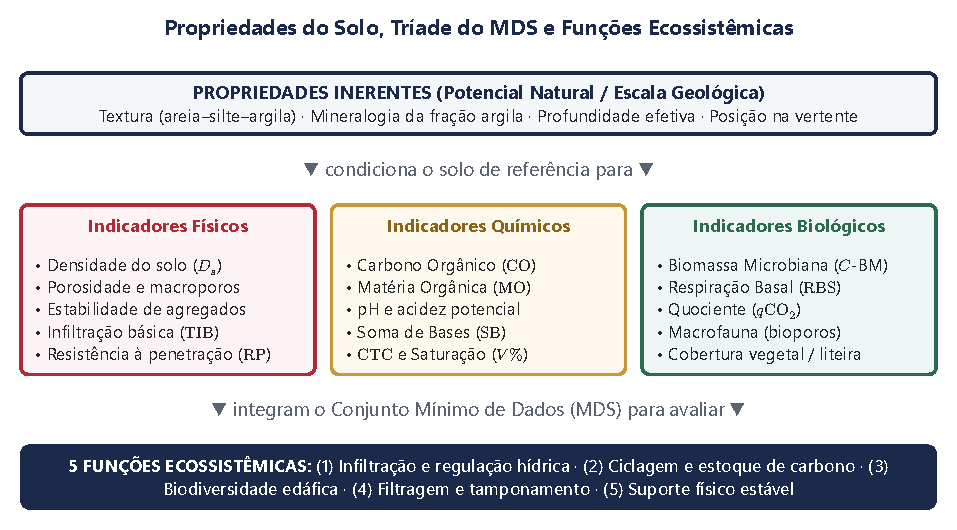
\includegraphics[width=0.92\textwidth]{figures/fig_cap11_triade_mds_funcoes.pdf}
  \caption{Relação entre propriedades inerentes do solo, tríade de indicadores dinâmicos do Conjunto Mínimo de Dados (MDS) e as cinco funções ecossistêmicas avaliadas.}
  \label{fig:triade_mds_funcoes}
\end{figure}

\section{Indicadores Físicos, Químicos e Biológicos do MDS}

\subsection{Indicadores Físicos (Arquitetura Porosa e Fluxo Hídrico)}

Os atributos físicos governam a circulação de água, ar e raízes no perfil edáfico e respondem rapidamente à degradação mecânica observada em pastagens sobrepastoreadas, áreas agrícolas convencionais e acessos de obras civis ou parques eólicos. A \textbf{densidade do solo ($D_s$)} mede a massa de solo seco contida em um volume conhecido de solo estruturado. Para preservar os poros originais sem esmagá-los, coleta-se uma amostra indeformada cravando um cilindro metálico de volume conhecido $V_t$ (anel de Kopecky) no perfil, levando-o à estufa a $105\,^\circ\text{C}$ até massa constante ($m_s$). Quanto maior a compactação imposta pelo tráfego ou pisoteio, mais partículas sólidas são comprimidas no mesmo volume e maior fica $D_s$. Solos minerais conservados exibem tipicamente valores entre $1{,}00$ e $1{,}35\text{ g}\cdot\text{cm}^{-3}$, ao passo que leituras acima de $1{,}55$--$1{,}65\text{ g}\cdot\text{cm}^{-3}$ em solos de textura média a argilosa costumam impor restrição severa ao crescimento radicular.

Para compreender o efeito real dessa compactação sobre a água e o ar, analisa-se a \textbf{porosidade total ($P_t$)} em conjunto com a separação entre \textbf{macroporosidade e microporosidade} (Figura~\ref{fig:porosidade_compactacao}). Na mesa de tensão a $6\text{ kPa}$, drenam-se os \textbf{macroporos} ($> 50\,\mu\text{m}$), responsáveis pela aeração das raízes e pela drenagem rápida da água gravitacional, restando retida a água dos \textbf{microporos} ($< 50\,\mu\text{m}$), que armazenam umidade disponível às plantas. Quando o solo sofre compressão mecânica, os macroporos colapsam primeiro, e valores de macroporosidade inferiores a $10\%$ do volume total tornam-se críticos para a oxigenação radicular.

\begin{figure}[H]
  \centering
  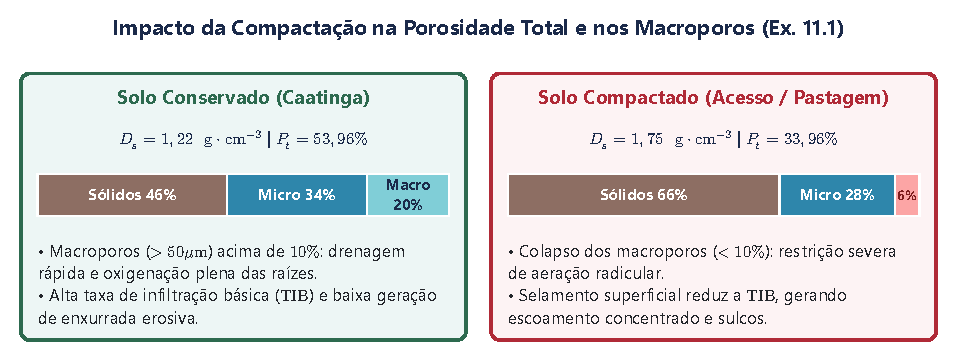
\includegraphics[width=0.92\textwidth]{figures/fig_cap11_porosidade_compactacao.pdf}
  \caption{Impacto da compactação na proporção volumétrica entre sólidos, microporos e macroporos, comparando Caatinga conservada e acesso compactado.}
  \label{fig:porosidade_compactacao}
\end{figure}

A integridade dessa arquitetura porosa depende da \textbf{estabilidade de agregados em água}, medida pelo Diâmetro Médio Ponderado (DMP) após peneiramento úmido. Agregados estáveis resistem ao impacto das gotas de chuva (\textit{splash}), prevenindo o selamento superficial. Quando o selamento ocorre ou os macroporos diminuem, cai abruptamente a \textbf{Taxa de Infiltração Básica ($TIB$)}, medida em campo com infiltrômetro de anéis concêntricos ($\text{mm}\cdot\text{h}^{-1}$), convertendo chuvas moderadas em escoamento superficial concentrado e sulcos erosivos (Figura~\ref{fig:solo_compactado_sulco}). Complementando essa leitura hidráulica, a \textbf{resistência do solo à penetração ($RP$)}, medida com penetrômetro ($\text{MPa}$), avalia o impedimento mecânico às raízes; na capacidade de campo, valores acima de $2{,}0$--$2{,}5\text{ MPa}$ restringem o alongamento radicular.

\begin{figure}[H]
  \centering
  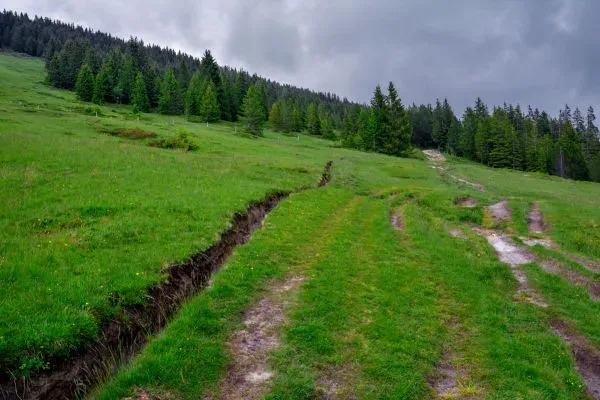
\includegraphics[width=0.78\textwidth]{figures/foto_estrada_sulco_erosivo.jpg}
  \caption{Superfície de solo compactado em acesso rural com selamento superficial, perda de macroporosidade e formação de sulco erosivo por escoamento superficial concentrado. Fonte: acervo didático da disciplina.}
  \label{fig:solo_compactado_sulco}
\end{figure}

As expressões físicas abaixo permitem quantificar densidade, porosidade total e frações porosas a partir do anel saturado ($m_{\text{sat}}$), drenado a $6\text{ kPa}$ ($m_{6\text{kPa}}$) e seco em estufa ($m_s$), com $\rho_{\text{água}} = 1{,}0\text{ g}\cdot\text{cm}^{-3}$:
\[
D_s = \frac{m_s}{V_t} \quad (\text{g}\cdot\text{cm}^{-3}) \qquad\qquad P_t = \left(1 - \frac{D_s}{D_p}\right) \times 100\%
\]
\[
P_{\text{micro}} = \frac{m_{6\text{kPa}} - m_s}{\rho_{\text{água}} \cdot V_t}\times 100\% \qquad\qquad P_{\text{macro}} = \frac{m_{\text{sat}} - m_{6\text{kPa}}}{\rho_{\text{água}} \cdot V_t}\times 100\%
\]

O Exemplo 11.1 aplica diretamente as relações de densidade e porosidade total aos dados representados na Figura~\ref{fig:porosidade_compactacao}.

\begin{boxExemplo}{11.1 (Básico)}{Cálculo de Densidade do Solo e Porosidade Total em Anel Volumétrico}
\passoEnunciado{Durante uma campanha prática da disciplina CHF662, foram coletadas amostras indeformadas ($0$--$10\text{ cm}$) utilizando anéis de Kopecky de $100\text{ cm}^3$ em um fragmento de Caatinga conservada e na borda compactada de um acesso de parque eólico ($D_p = 2{,}65\text{ g}\cdot\text{cm}^{-3}$).}
\passoDados{Volume $V_t = 100\text{ cm}^3$; massa seca na Caatinga $m_{s,1} = 122\text{ g}$; massa seca no acesso compactado $m_{s,2} = 175\text{ g}$.}
\passoPedido{Calcular a densidade do solo ($D_s$) e a porosidade total ($P_t$) em ambos os pontos e interpretar o contraste físico.}
\passoMetodo{Aplicação direta das expressões $D_s = m_s / V_t$ e $P_t = (1 - D_s / D_p)\times 100\%$.}
\passoContas{
\[
D_{s,1} = \frac{122}{100} = 1{,}22\text{ g}\cdot\text{cm}^{-3} \quad\Rightarrow\quad P_{t,1} = \left(1 - \frac{1{,}22}{2{,}65}\right)\times 100\% = 53{,}96\%
\]
\[
D_{s,2} = \frac{175}{100} = 1{,}75\text{ g}\cdot\text{cm}^{-3} \quad\Rightarrow\quad P_{t,2} = \left(1 - \frac{1{,}75}{2{,}65}\right)\times 100\% = 33{,}96\%
\]
Diferença: $P_{t,2} - P_{t,1} = -20{,}00$ pontos percentuais (perda relativa de $37{,}1\%$ do espaço poroso).}
\passoResposta{Caatinga conservada: $D_s = 1{,}22\text{ g}\cdot\text{cm}^{-3}$ e $P_t = 53{,}96\%$. Acesso compactado: $D_s = 1{,}75\text{ g}\cdot\text{cm}^{-3}$ e $P_t = 33{,}96\%$.}
\passoVerificacao{A compactação aumentou $D_s$ em $0{,}53\text{ g}\cdot\text{cm}^{-3}$ e eliminou $20$ pontos percentuais de porosidade, colapsando prioritariamente os macroporos de drenagem rápida.}
\end{boxExemplo}

Quando o diagnóstico físico inclui medições em mesa de tensão, quantifica-se separadamente quanto dessa porosidade total permanece disponível para aeração radicular, conforme mostra o Exemplo 11.4.

\begin{boxExemplo}{11.4 (Avançado)}{Separação de Macro e Microporosidade em Mesa de Tensão}
\passoEnunciado{Uma amostra indeformada de solo ($V_t = 100\text{ cm}^3$) proveniente de uma área em recuperação com bioengenharia foi saturada por capilaridade, submetida à tensão de $6\text{ kPa}$ em mesa de tensão e, finalmente, seca em estufa a $105\,^\circ\text{C}$.}
\passoDados{$V_t = 100\text{ cm}^3$; $\rho_{\text{água}} = 1{,}0\text{ g}\cdot\text{cm}^{-3}$. Massas (descontada a tara): $m_{\text{sat}} = 174\text{ g}$; $m_{6\text{kPa}} = 158\text{ g}$; $m_s = 128\text{ g}$.}
\passoPedido{Determinar $P_t^{\text{sat}}$, $P_{\text{micro}}$ e $P_{\text{macro}}$, avaliando se há restrição de aeração radicular.}
\passoMetodo{Cálculo dos volumes de água retidos em cada estado energético divididos pelo volume do anel.}
\passoContas{
\begin{align*}
P_t^{\text{sat}} &= \frac{174 - 128}{100}\times 100\% = 46{,}0\% \\
P_{\text{micro}} &= \frac{158 - 128}{100}\times 100\% = 30{,}0\% \qquad P_{\text{macro}} = \frac{174 - 158}{100}\times 100\% = 16{,}0\%
\end{align*}
Conferência aditiva: $P_{\text{micro}} + P_{\text{macro}} = 30{,}0\% + 16{,}0\% = 46{,}0\% = P_t^{\text{sat}}$.}
\passoResposta{$P_t^{\text{sat}} = 46{,}0\%$, $P_{\text{micro}} = 30{,}0\%$ e $P_{\text{macro}} = 16{,}0\%$, superando o limiar mínimo de $10\%$ sem restrição crítica à aeração.}
\passoVerificacao{A proporção de cerca de um terço de macroporos e dois terços de microporos aproxima-se do equilíbrio físico desejável para armazenamento hídrico aliado à drenagem interna.}
\end{boxExemplo}

Na interpretação de campo dos indicadores físicos, dois equívocos metodológicos comprometem os laudos de degradação: comparar solos de texturas distintas sem referência local e medir resistência à penetração sem registrar a umidade.

\begin{boxErro}[Erro 1: Comparar Áreas em Solos de Texturas Distintas Sem Referência Local]
\textbf{Equívoco frequente:} Classificar um Neossolo Quartzarênico arenoso ($D_s = 1{,}45\text{ g}\cdot\text{cm}^{-3}$) como degradado comparando-o a um Latossolo argiloso conservado ($D_s = 1{,}05\text{ g}\cdot\text{cm}^{-3}$).\par
\textbf{Correção técnica:} Solos arenosos possuem naturalmente maior densidade e menor $CTC$ do que solos argilosos bem estruturados. A área de referência sob vegetação nativa deve pertencer à \textbf{mesma classe de solo, textura e posição geomorfológica} da área diagnosticada.
\end{boxErro}

No Semiárido, a sazonalidade hídrica amplia drasticamente a coesão aparente do solo seco, exigindo cuidado adicional nas leituras de penetrômetro.

\begin{boxErro}[Erro 2: Avaliar Resistência à Penetração ($RP$) Sem Registrar a Umidade do Solo]
\textbf{Equívoco frequente:} Medir $RP$ na estação seca no Semiárido, obter valores acima de $4{,}0\text{ MPa}$ e diagnosticar compactação antrópica irreversível.\par
\textbf{Correção técnica:} A resistência mecânica à penetração aumenta exponencialmente à medida que o solo seca, devido à coesão entre partículas e à sucção matricial. Leituras de penetrômetro só são comparáveis quando realizadas sob umidade controlada (próxima à capacidade de campo) ou acompanhadas do teor gravimétrico de umidade.
\end{boxErro}

\subsection{Indicadores Químicos (Matéria Orgânica, Acidez e Troca Catiônica)}

Os atributos químicos determinam a disponibilidade de nutrientes, o poder tampão e a estabilidade coloidal do solo. Nesse compartimento, a \textbf{Matéria Orgânica ($MO$)} e o \textbf{Carbono Orgânico Total ($CO$)} integram física, química e biologia porque cimentam agregados, elevam a retenção de água e fornecem a maior parte das cargas negativas responsáveis pela $CTC$ em solos tropicais intemperizados. Como os métodos laboratoriais (Walkley--Black ou combustão seca) quantificam diretamente o carbono orgânico ($CO$), estima-se a matéria orgânica multiplicando $CO$ pelo \textbf{fator de van Bemmelen ($1{,}724$)}, baseado na convenção de que a matéria orgânica humificada contém aproximadamente $58\%$ de carbono em massa ($1 / 0{,}58 \approx 1{,}724$). As equações químicas abaixo permitem converter $CO$ em $MO$ e calcular o estoque de carbono ($EC$, em $\text{Mg C}\cdot\text{ha}^{-1}$) na camada de espessura $h_{\text{m}}$ (utilizando $1\text{ g}\cdot\text{cm}^{-3} = 1\text{ Mg}\cdot\text{m}^{-3}$):
\[
CO = \frac{MO}{1{,}724} \quad \Longleftrightarrow \quad MO = CO \times 1{,}724 \qquad\qquad EC = \left(\frac{CO_{\text{g/kg}}}{1000}\right) \cdot D_s \cdot (10.000 \cdot h_{\text{m}})
\]

O Exemplo 11.2 demonstra como padronizar laudos expressos em grandezas distintas e quantificar a perda de carbono por hectare.

\begin{boxExemplo}{11.2 (Básico/Intermediário)}{Fator de van Bemmelen e Estoque de Carbono na Camada 0--20 cm}
\passoEnunciado{Um laudo laboratorial reportou carbono orgânico total de $18{,}0\text{ g}\cdot\text{kg}^{-1}$ em um solo sob Caatinga preservada (Área A, $D_s = 1{,}25\text{ g}\cdot\text{cm}^{-3}$). Em uma pastagem degradada adjacente no mesmo solo (Área B, $D_s = 1{,}60\text{ g}\cdot\text{cm}^{-3}$), outro laboratório expressou o resultado em matéria orgânica total, $MO = 12{,}068\text{ g}\cdot\text{kg}^{-1}$.}
\passoDados{Camada $h = 0{,}20\text{ m}$. Área A: $CO_A = 18{,}0\text{ g}\cdot\text{kg}^{-1}$, $D_{s,A} = 1{,}25$. Área B: $MO_B = 12{,}068\text{ g}\cdot\text{kg}^{-1}$, $D_{s,B} = 1{,}60$. Fator de van Bemmelen: $1{,}724$.}
\passoPedido{Calcular o teor de $MO$ na Área A, o teor de $CO$ na Área B, o estoque de carbono ($EC$, em $\text{Mg C}\cdot\text{ha}^{-1}$) nas duas áreas e a perda líquida de carbono.}
\passoMetodo{Conversão via fator de van Bemmelen ($MO = 1{,}724 \cdot CO$) e cálculo da massa de solo por hectare na camada de $0{,}20\text{ m}$.}
\passoContas{
\[
MO_A = 18{,}0 \times 1{,}724 = 31{,}032\text{ g}\cdot\text{kg}^{-1} \quad (3{,}10\%) \qquad\qquad CO_B = \frac{12{,}068}{1{,}724} = 7{,}00\text{ g}\cdot\text{kg}^{-1} \quad (0{,}70\%)
\]
Volume em $1\text{ ha}$ ($0{,}20\text{ m}$): $V_{\text{ha}} = 2.000\text{ m}^3\cdot\text{ha}^{-1}$.
Área A: massa $= 2.000 \times 1{,}25 = 2.500\text{ Mg}\cdot\text{ha}^{-1} \Rightarrow EC_A = 2.500 \times 0{,}018 = 45{,}00\text{ Mg C}\cdot\text{ha}^{-1}$.
Área B: massa $= 2.000 \times 1{,}60 = 3.200\text{ Mg}\cdot\text{ha}^{-1} \Rightarrow EC_B = 3.200 \times 0{,}007 = 22{,}40\text{ Mg C}\cdot\text{ha}^{-1}$.
Perda líquida: $\Delta EC = 45{,}00 - 22{,}40 = 22{,}60\text{ Mg C}\cdot\text{ha}^{-1}$ ($-50{,}2\%$).}
\passoResposta{Área A: $MO = 31{,}032\text{ g}\cdot\text{kg}^{-1}$ e $EC = 45{,}00\text{ Mg C}\cdot\text{ha}^{-1}$. Área B: $CO = 7{,}00\text{ g}\cdot\text{kg}^{-1}$ e $EC = 22{,}40\text{ Mg C}\cdot\text{ha}^{-1}$. Perda líquida de $22{,}60\text{ Mg C}\cdot\text{ha}^{-1}$.}
\passoVerificacao{Mesmo com maior massa de solo em $20\text{ cm}$ na Área B devido à compactação ($3.200$ vs. $2.500\text{ Mg}$), a perda já ultrapassa metade do estoque original.}
\end{boxExemplo}

Na comparação entre laudos laboratoriais diferentes, um erro frequente decorre da troca direta entre carbono orgânico e matéria orgânica sem aplicar o fator de conversão.

\begin{boxErro}[Erro 3: Confundir Carbono Orgânico ($CO$) com Matéria Orgânica ($MO$)]
\textbf{Equívoco frequente:} Comparar diretamente um laudo expresso em $CO$ ($\text{g}\cdot\text{kg}^{-1}$) com outro expresso em $MO$ ($\text{g}\cdot\text{kg}^{-1}$) sem conversão prévia.\par
\textbf{Correção técnica:} A matéria orgânica contém carbono, oxigênio, hidrogênio e nitrogênio; portanto, $MO$ é sempre numericamente maior que $CO$ ($MO = 1{,}724 \times CO$). Padronize todas as amostras na mesma grandeza antes de comparar resultados ou calcular estoques de carbono.
\end{boxErro}

O \textbf{potencial hidrogeniônico (pH)} controla a solubilidade de nutrientes e a toxicidade do alumínio trocável ($Al^{3+}$) abaixo de pH $5{,}5$. No Semiárido Baiano, Luvissolos e Neossolos pouco intemperizados tendem a apresentar pH levemente ácido a neutro ($6{,}0$--$7{,}2$), enquanto Latossolos profundos de tabuleiros costumam ser mais ácidos ($4{,}5$--$5{,}5$). Associando a \textbf{Soma de Bases ($SB$)} à acidez potencial ($H^+ + Al^{3+}$), obtém-se a $CTC$ a pH $7{,}0$ e a \textbf{Saturação por Bases ($V\%$)}:
\[
SB = Ca^{2+} + Mg^{2+} + K^+ + Na^+ \qquad CTC = SB + (H^+ + Al^{3+}) \qquad V\% = \frac{SB}{CTC}\times 100\%
\]
Solos com $V\% \ge 50\%$ são classificados como \textbf{eutróficos} (alta fertilidade natural), ao passo que solos com $V\% < 50\%$ são \textbf{distróficos} (baixa fertilidade natural). O Exemplo 11.3 contrasta essas duas classes pedológicas na Bahia.

\begin{boxExemplo}{11.3 (Intermediário)}{Diagnóstico Químico: Soma de Bases, CTC e Saturação por Bases ($V\%$)}
\passoEnunciado{Compare os laudos químicos de rotina (camada $0$--$20\text{ cm}$) de dois solos baianos: Solo 1 (Luvissolo Crômico sob Caatinga no Semiárido) e Solo 2 (Latossolo Amarelo sob pastagem degradada nos Tabuleiros Costeiros).}
\passoDados{Valores em $\text{cmol}_c\cdot\text{dm}^{-3}$. Solo 1: $Ca^{2+} = 5{,}40$; $Mg^{2+} = 2{,}60$; $K^+ = 0{,}45$; $Na^+ = 0{,}15$; $H^+ + Al^{3+} = 2{,}40$. Solo 2: $Ca^{2+} = 1{,}20$; $Mg^{2+} = 0{,}60$; $K^+ = 0{,}15$; $Na^+ = 0{,}05$; $H^+ + Al^{3+} = 4{,}00$.}
\passoPedido{Calcular $SB$, $CTC$ a pH $7{,}0$ e $V\%$ para os dois solos e classificá-los quanto ao caráter eutrófico ou distrófico.}
\passoMetodo{Aplicação das equações aditivas de $SB$ e $CTC$ e cálculo da razão percentual $V\% = (SB / CTC)\times 100\%$.}
\passoContas{
\begin{align*}
SB_1 &= 8{,}60\text{ cmol}_c\cdot\text{dm}^{-3} \qquad & CTC_1 &= 8{,}60 + 2{,}40 = 11{,}00\text{ cmol}_c\cdot\text{dm}^{-3} \\
V\%_1 &= \frac{8{,}60}{11{,}00}\times 100\% = 78{,}18\% & & \\[4pt]
SB_2 &= 2{,}00\text{ cmol}_c\cdot\text{dm}^{-3} \qquad & CTC_2 &= 2{,}00 + 4{,}00 = 6{,}00\text{ cmol}_c\cdot\text{dm}^{-3} \\
V\%_2 &= \frac{2{,}00}{6{,}00}\times 100\% = 33{,}33\% & &
\end{align*}}
\passoResposta{Solo 1: $SB = 8{,}60$, $CTC = 11{,}00\text{ cmol}_c\cdot\text{dm}^{-3}$ e $V\% = 78{,}18\%$ (eutrófico). Solo 2: $SB = 2{,}00$, $CTC = 6{,}00\text{ cmol}_c\cdot\text{dm}^{-3}$ e $V\% = 33{,}33\%$ (distrófico).}
\passoVerificacao{No Semiárido, a menor lixiviação preserva bases trocáveis, enquanto nos ambientes úmidos a intensa lixiviação combinada à perda de matéria orgânica reduz $SB$, $CTC$ e $V\%$.}
\end{boxExemplo}

\subsection{Indicadores Biológicos (Motor Vivo da Funcionalidade Edáfica)}

Os indicadores biológicos costumam responder às perturbações iniciais e às ações de recuperação antes que os estoques totais de carbono ou a densidade exibam alterações mensuráveis. O \textbf{Carbono da Biomassa Microbiana ($C\text{-BM}$)} representa a fração viva da matéria orgânica (fungos, bactérias e actinomicetos, geralmente entre $1\%$ e $4\%$ do $CO$ total) e reage em poucos meses ao manejo. Interpretado junto à \textbf{Respiração Basal do Solo ($RBS$)}, que mede a liberação de $\text{CO}_2$ pela atividade metabólica, o quociente metabólico ($q\text{CO}_2 = RBS / C\text{-BM}$) funciona como termômetro de estresse ecológico: valores elevados indicam que os microrganismos gastam mais energia na manutenção celular do que no crescimento. Completa esse eixo a \textbf{fauna edáfica e a cobertura vegetal}, pois minhocas, térmitas e formigas constroem bioporos enquanto a serapilheira amortece a temperatura superficial. Em pastagens degradadas sem cobertura vegetal, a atividade biológica entra em colapso e o solo exposto evolui rapidamente para ravinas (Figura~\ref{fig:pastagem_ravinas}).

\begin{figure}[H]
  \centering
  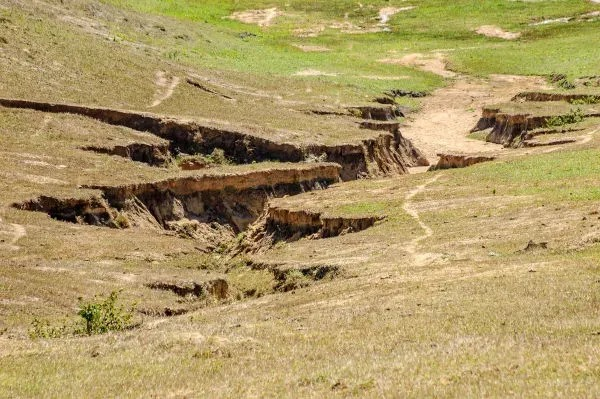
\includegraphics[width=0.78\textwidth]{figures/foto_pastagem_ravinas.jpg}
  \caption{Pastagem degradada com perda de cobertura vegetal, exposição do horizonte mineral e evolução de ravinas em vertente. Fonte: acervo didático da disciplina.}
  \label{fig:pastagem_ravinas}
\end{figure}

\section{Normalização Linear, Cálculo do IQS e Visualização Multivariada}

Como cada indicador possui unidade distinta ($\text{g}\cdot\text{kg}^{-1}$, $\text{mm}\cdot\text{h}^{-1}$, $\text{g}\cdot\text{cm}^{-3}$), converte-se cada valor bruto $x_i$ em uma nota adimensional $S_i \in [0, 1]$ para viabilizar a agregação matemática (Figura~\ref{fig:curvas_normalizacao}). Para atributos cuja elevação favorece a funcionalidade edáfica (\textbf{``quanto maior melhor''}, como $MO$, $P_t$, $TIB$ e $DMP$), aplica-se $S_i = \min\!\left(1;\; \dfrac{x_i}{x_{\text{ref}}}\right)$, travando a nota máxima em $1{,}0$. Para atributos cujo aumento indica restrição física (\textbf{``quanto menor melhor''}, como $D_s$ e $RP$), inverte-se a razão, $S_i = \min\!\left(1;\; \dfrac{x_{\text{ref}}}{x_i}\right)$.

\begin{figure}[H]
  \centering
  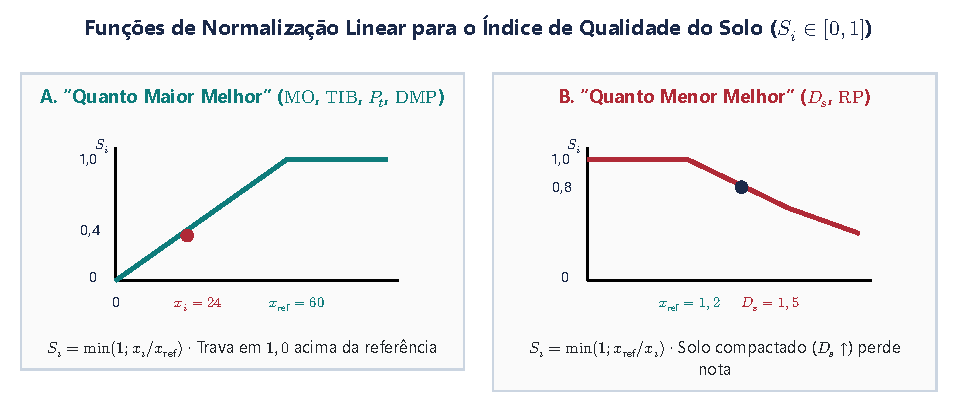
\includegraphics[width=0.92\textwidth]{figures/fig_cap11_curvas_normalizacao.pdf}
  \caption{Curvas das funções de normalização linear para indicadores ``quanto maior melhor'' (A) e ``quanto menor melhor'' (B), mostrando os pontos de referência e o comportamento fora da faixa ótima.}
  \label{fig:curvas_normalizacao}
\end{figure}

Agregando as pontuações $S_i$, calcula-se o Índice de Qualidade do Solo simples ou ponderado:
\[
\text{IQS}_{\text{simples}} = \frac{1}{n}\sum_{i=1}^{n} S_i \qquad \text{ou} \qquad \text{IQS}_{\text{ponderado}} = \sum_{i=1}^{n} w_i \, S_i \quad \left(\text{com } \sum_{i=1}^{n} w_i = 1\right)
\]

A integração dessas notas normalizadas em um \textbf{gráfico radar} (Figura~\ref{fig:qualidade_solo_radar}) preserva simultaneamente a visão global (área do polígono proporcional ao IQS) e o diagnóstico individual de cada gargalo (eixos recolhidos próximo ao centro).

\begin{figure}[H]
  \centering
  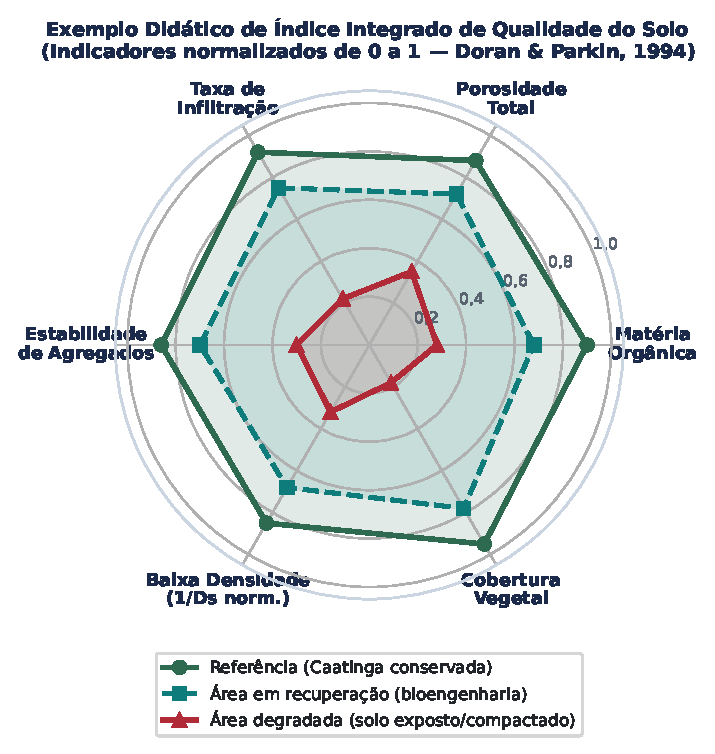
\includegraphics[width=0.80\textwidth]{figures/fig09_qualidade_solo_radar.pdf}
  \caption{Comparação multivariada de seis indicadores normalizados de qualidade do solo ($0$ a $1$) entre área de referência sob Caatinga conservada, área em recuperação com técnicas de bioengenharia e área degradada com solo exposto e compactado.}
  \label{fig:qualidade_solo_radar}
\end{figure}

Observando os cenários plotados (Figura~\ref{fig:qualidade_solo_radar}), a \textbf{área de referência sob Caatinga conservada} apresenta escores entre $0{,}85$ e $0{,}95$, resultando em $\text{IQS} = (0{,}90+0{,}88+0{,}92+0{,}86+0{,}85+0{,}95)/6 = \mathbf{0{,}893}$ (qualidade muito alta). A \textbf{área em recuperação com bioengenharia} alcança escores entre $0{,}68$ e $0{,}78$, com $\text{IQS} = \mathbf{0{,}718}$ (trajetória ascendente, com matéria orgânica e densidade ainda em consolidação). Já a \textbf{área degradada} exibe escores colapsados entre $0{,}18$ (cobertura vegetal) e $0{,}35$ (porosidade total), produzindo $\text{IQS} = \mathbf{0{,}275}$ e demandando intervenção prioritária na cobertura superficial e descompactação biológica.

\etapa{4}{Síntese Integrada do Índice de Qualidade do Solo}

O Exemplo 11.5 consolida a passagem completa das medições brutas em campo e laboratório até o cálculo dos índices simples e ponderado.

\begin{boxExemplo}{11.5 (Avançado)}{Normalização Linear e Cálculo Completo do Índice de Qualidade do Solo (IQS)}
\passoEnunciado{Para o Trabalho Prático Final, um grupo selecionou quatro indicadores para avaliar uma encosta submetida à recuperação ambiental frente a uma mata de referência no mesmo solo.}
\passoDados{$MO$ (``maior melhor''): avaliada $= 16{,}0\text{ g}\cdot\text{kg}^{-1}$, ref. $= 32{,}0$, $w_1 = 0{,}30$; $TIB$ (``maior melhor''): avaliada $= 24{,}0\text{ mm}\cdot\text{h}^{-1}$, ref. $= 60{,}0$, $w_2 = 0{,}30$; $D_s$ (``menor melhor''): avaliada $= 1{,}50\text{ g}\cdot\text{cm}^{-3}$, ref. $= 1{,}20$, $w_3 = 0{,}20$; $DMP$ (``maior melhor''): avaliada $= 1{,}25\text{ mm}$, ref. $= 2{,}50$, $w_4 = 0{,}20$.}
\passoPedido{Calcular a pontuação normalizada $S_i$ de cada indicador, o $\text{IQS}_{\text{simples}}$ e o $\text{IQS}_{\text{ponderado}}$, indicando o gargalo prioritário.}
\passoMetodo{Normalização linear conforme as curvas da Figura~\ref{fig:curvas_normalizacao} seguida das médias aritmética e ponderada.}
\passoContas{
\begin{align*}
  S_{MO} &= \frac{16{,}0}{32{,}0} = 0{,}50 \qquad & S_{TIB} &= \frac{24{,}0}{60{,}0} = 0{,}40 \\
  S_{D_s} &= \frac{1{,}20}{1{,}50} = 0{,}80 \;\text{(invertida)} \qquad & S_{DMP} &= \frac{1{,}25}{2{,}50} = 0{,}50
\end{align*}
\begin{align*}
  \text{IQS}_{\text{simples}} &= \frac{0{,}50 + 0{,}40 + 0{,}80 + 0{,}50}{4} = 0{,}550 \\
  \text{IQS}_{\text{ponderado}} &= (0{,}30 \times 0{,}50) + (0{,}30 \times 0{,}40) + (0{,}20 \times 0{,}80) + (0{,}20 \times 0{,}50) = 0{,}530
\end{align*}}
\passoResposta{Pontuações: $S_{MO}=0{,}50$, $S_{TIB}=0{,}40$, $S_{D_s}=0{,}80$, $S_{DMP}=0{,}50$. $\text{IQS}_{\text{simples}} = 0{,}550$ e $\text{IQS}_{\text{ponderado}} = 0{,}530$ (qualidade moderada). O gargalo prioritário é a taxa de infiltração básica ($S_{TIB} = 0{,}40$).}
\passoVerificacao{O $\text{IQS}_{\text{ponderado}}$ ($0{,}530$) ficou abaixo do simples ($0{,}550$) porque os maiores pesos ($0{,}30$) recaíram sobre infiltração e matéria orgânica, orientando ações focadas em cobertura morta e aporte orgânico.}
\end{boxExemplo}

\etapa{5}{Cuidado Final na Normalização e Materiais Audiovisuais de Apoio}

Ao calcular o IQS em planilhas eletrônicas, verifique sempre o sentido da função de normalização antes de gerar o gráfico radar, evitando o erro algébrico descrito a seguir.

\begin{boxErro}[Erro 4: Usar a Fórmula ``Quanto Maior Melhor'' para Densidade do Solo ($D_s$)]
\textbf{Equívoco frequente:} Normalizar $D_s$ dividindo o valor da área degradada ($1{,}75$) pelo da referência ($1{,}20$), obtendo escore superior a $1{,}0$ e premiando um solo severamente compactado.\par
\textbf{Correção técnica:} Para densidade do solo e resistência à penetração, valores maiores indicam pior qualidade física. Aplica-se obrigatoriamente a função \textbf{``quanto menor melhor''}: $S_{D_s} = \min(1;\; D_{s,\text{ref}} / D_{s,\text{avaliado}})$.
\end{boxErro}

Para consolidar a visualização dos indicadores físicos, químicos e biológicos em campo e laboratório, consulte os vídeos selecionados na página da disciplina: \textit{Análise da Saúde do Solo} (\url{https://www.youtube.com/watch?v=D8jI-ltuzVI}, cerca de 7 min, integrando matéria orgânica, densidade, porosidade e biologia edáfica), \textit{Saúde do Solo: Qualidade Biológica} (\url{https://www.youtube.com/watch?v=WHh50dAM4as}, focado em indicadores biológicos tropicais) e \textit{Degradação dos Solos} (\url{https://www.youtube.com/watch?v=QujBcIOl3qQ}, cerca de 17 min, ilustrando lixiviação, erosão, laterização e salinização).

\etapa{6}{Exercícios de Fixação}

\subsection*{Nível Básico (Conceitos de Funcionalidade Edáfica e MDS)}

\begin{enumerate}[leftmargin=1.8em, itemsep=6pt]
  \item Explique por que o conceito contemporâneo de \textbf{Qualidade do Solo} (Doran; Parkin, 1994; Karlen et al., 1997) é mais abrangente do que a noção tradicional de fertilidade química agrícola.
  \espacoResolucao[1.8cm]

  \item Diferencie \textbf{propriedades inerentes} de \textbf{propriedades dinâmicas} do solo, citando dois exemplos de cada grupo.
  \espacoResolucao[1.8cm]

  \item Qual é o significado físico e matemático do \textbf{fator de van Bemmelen ($1{,}724$)} na conversão entre carbono orgânico total ($CO$) e matéria orgânica ($MO$)?
  \espacoResolucao[1.8cm]

  \item Por que a \textbf{macroporosidade} é mais sensível à compactação do solo do que a porosidade total ($P_t$), e qual é o seu limiar crítico de aeração radicular?
  \espacoResolucao[1.8cm]

  \item Explique por que o \textbf{Carbono da Biomassa Microbiana ($C\text{-BM}$)} e o quociente metabólico ($q\text{CO}_2$) são indicadores precoces valiosos no monitoramento de áreas degradadas em recuperação.
  \espacoResolucao[1.8cm]
\end{enumerate}

\subsection*{Nível Intermediário (Cálculos Físicos, Químicos e IQS)}

\begin{enumerate}[leftmargin=1.8em, itemsep=6pt, resume]
  \item Uma amostra indeformada coletada em anel volumétrico de $100\text{ cm}^3$ apresentou massa de solo seco em estufa de $159\text{ g}$. Considerando densidade de partículas $D_p = 2{,}65\text{ g}\cdot\text{cm}^{-3}$, calcule a densidade do solo ($D_s$) e a porosidade total ($P_t$).
  \espacoResolucao[2.2cm]

  \item Um solo sob Caatinga em regeneração apresentou teor de matéria orgânica $MO = 25{,}86\text{ g}\cdot\text{kg}^{-1}$ e densidade do solo $D_s = 1{,}30\text{ g}\cdot\text{cm}^{-3}$ na camada $0$--$20\text{ cm}$. Calcule o teor de carbono orgânico total ($CO$, em $\text{g}\cdot\text{kg}^{-1}$) usando o fator de van Bemmelen e o estoque de carbono ($EC$, em $\text{Mg C}\cdot\text{ha}^{-1}$) nessa camada.
  \espacoResolucao[2.2cm]

  \item Um laudo químico forneceu os seguintes valores (em $\text{cmol}_c\cdot\text{dm}^{-3}$): $Ca^{2+} = 4{,}20$; $Mg^{2+} = 1{,}80$; $K^+ = 0{,}30$; $Na^+ = 0{,}10$; e $H^+ + Al^{3+} = 3{,}60$. Calcule $SB$, $CTC$ e $V\%$, classificando o solo como eutrófico ou distrófico.
  \espacoResolucao[2.2cm]

  \item Em ensaio de mesa de tensão com anel de $100\text{ cm}^3$ ($\rho_{\text{água}} = 1{,}0\text{ g}\cdot\text{cm}^{-3}$), obtiveram-se as massas (sem a tara do anel): $m_{\text{sat}} = 165\text{ g}$, $m_{6\text{kPa}} = 157\text{ g}$ e $m_s = 130\text{ g}$. Calcule $P_t^{\text{sat}}$, $P_{\text{micro}}$ e $P_{\text{macro}}$, indicando se há risco físico à aeração das raízes.
  \espacoResolucao[2.2cm]

  \item Calcule o $\text{IQS}_{\text{simples}}$ de uma parcela degradada a partir dos três indicadores abaixo e identifique o indicador de menor desempenho:
  \begin{itemize}[leftmargin=1.4em, itemsep=1pt]
    \item $MO$ (maior melhor): parcela $= 20\text{ g}\cdot\text{kg}^{-1}$; referência $= 40\text{ g}\cdot\text{kg}^{-1}$.
    \item $TIB$ (maior melhor): parcela $= 36\text{ mm}\cdot\text{h}^{-1}$; referência $= 60\text{ mm}\cdot\text{h}^{-1}$.
    \item $D_s$ (menor melhor): parcela $= 1{,}60\text{ g}\cdot\text{cm}^{-3}$; referência $= 1{,}20\text{ g}\cdot\text{cm}^{-3}$.
  \end{itemize}
  \espacoResolucao[2.2cm]
\end{enumerate}

\subsection*{Nível Aplicado (Questões Objetivas A--E)}

\begin{enumerate}[leftmargin=1.8em, itemsep=6pt, resume]
  \item A respeito do Conjunto Mínimo de Dados (MDS) para avaliação da qualidade do solo (Doran; Parkin, 1994; Vezzani; Mielniczuk, 2009), assinale a alternativa correta:
  \begin{alternativas}
    \item Deve conter apenas variáveis químicas de rotina, pois atributos físicos e biológicos não se alteram com o manejo da terra.
    \item Deve integrar um número enxuto e representativo de indicadores físicos, químicos e biológicos sensíveis às mudanças de uso da terra.
    \item Exige a medição simultânea de todos os 50 atributos laboratoriais existentes, independentemente de redundância ou custo.
    \item Dispensa a adoção de áreas de referência sob vegetação nativa por utilizar valores absolutos idênticos para qualquer textura de solo.
    \item Restringe-se ao estudo de solos hidromórficos de várzea.
  \end{alternativas}

  \item Um solo mineral com densidade de partículas $D_p = 2{,}65\text{ g}\cdot\text{cm}^{-3}$ e densidade do solo $D_s = 1{,}325\text{ g}\cdot\text{cm}^{-3}$ apresenta porosidade total ($P_t$) exatamente igual a:
  \begin{alternativas}
    \item $25{,}0\%$.
    \item $40{,}0\%$.
    \item $45{,}0\%$.
    \item $50{,}0\%$.
    \item $60{,}0\%$.
  \end{alternativas}

  \item Sobre a normalização de indicadores no cálculo do Índice de Qualidade do Solo (IQS), é correto afirmar que:
  \begin{alternativas}
    \item Indicadores como taxa de infiltração básica e matéria orgânica seguem a função ``quanto menor melhor''.
    \item A normalização converte grandezas com unidades diferentes para uma escala adimensional comum (como $0$ a $1$), possibilitando a agregação matemática.
    \item A densidade do solo deve ser normalizada pela razão $D_{s,\text{avaliado}} / D_{s,\text{referência}}$ para que solos mais compactados recebam notas maiores.
    \item O uso de pesos diferenciados ($w_i$) é proibido em índices de qualidade ambiental.
    \item Um IQS igual a $0{,}25$ indica funcionalidade edáfica superior à da área de referência.
  \end{alternativas}

  \item Se uma amostra de solo apresenta teor de carbono orgânico total $CO = 10{,}0\text{ g}\cdot\text{kg}^{-1}$, o teor estimado de matéria orgânica ($MO$) pelo fator de van Bemmelen ($1{,}724$) é:
  \begin{alternativas}
    \item $5{,}80\text{ g}\cdot\text{kg}^{-1}$.
    \item $10{,}00\text{ g}\cdot\text{kg}^{-1}$.
    \item $15{,}80\text{ g}\cdot\text{kg}^{-1}$.
    \item $17{,}24\text{ g}\cdot\text{kg}^{-1}$.
    \item $27{,}24\text{ g}\cdot\text{kg}^{-1}$.
  \end{alternativas}

  \item Na interpretação do gráfico radar de qualidade do solo (Figura~\ref{fig:qualidade_solo_radar}), uma área degradada que apresenta valores normalizados muito baixos em \textit{cobertura vegetal} ($0{,}18$) e \textit{taxa de infiltração} ($0{,}22$) sinaliza prioritariamente:
  \begin{alternativas}
    \item Alta resiliência física da superfície do solo frente a chuvas intensas.
    \item Predomínio de drenagem profunda com risco nulo de escoamento superficial.
    \item Forte vulnerabilidade ao impacto da gota de chuva, selamento superficial e geração de enxurrada erosiva.
    \item Excesso de matéria orgânica humificada na camada superficial.
    \item Equivalência funcional plena em relação à Caatinga conservada.
  \end{alternativas}
\end{enumerate}

\etapa{7}{Questões no Estilo ENADE e Concursos Ambientais}

\begin{boxDica}[Atenção às Armadilhas em Questões de Solos]
Em provas de Geografia e concursos ambientais, dois detalhes costumam decidir questões: verificar se a tabela fornece \textbf{Carbono Orgânico ($CO$)} ou \textbf{Matéria Orgânica ($MO$)} antes de multiplicar ou dividir por $1{,}724$, e observar o sentido da normalização (``maior melhor'' vs. ``menor melhor'') em indicadores como $D_s$ e $RP$.
\end{boxDica}

\begin{enumerate}[leftmargin=1.8em, itemsep=7pt]
  \item \textbf{[Questão Autoral, Estilo ENADE / Geografia]} Dois talhões localizados sobre a mesma classe de solo no Semiárido Baiano foram avaliados quanto à funcionalidade edáfica. O Talhão X (Caatinga conservada) exibiu $D_s = 1{,}20\text{ g}\cdot\text{cm}^{-3}$, $P_{\text{macro}} = 18\%$, $MO = 30\text{ g}\cdot\text{kg}^{-1}$ e $TIB = 65\text{ mm}\cdot\text{h}^{-1}$. O Talhão Y (área de empréstimo de terra após obra viária) apresentou $D_s = 1{,}72\text{ g}\cdot\text{cm}^{-3}$, $P_{\text{macro}} = 6\%$, $MO = 7\text{ g}\cdot\text{kg}^{-1}$ e $TIB = 9\text{ mm}\cdot\text{h}^{-1}$. Com base nesses resultados, analise as asserções:
  \begin{quote}
    \textbf{I.} O Talhão Y encontra-se fisicamente degradado e sob elevada suscetibilidade ao escoamento superficial concentrado e à erosão hídrica.\\
    \textbf{PORQUE}\\
    \textbf{II.} A perda de matéria orgânica e o colapso da macroporosidade abaixo de $10\%$ comprometem a estabilidade dos agregados e reduzem drasticamente a taxa de infiltração básica do solo.
  \end{quote}
  A respeito dessas asserções, assinale a opção correta:
  \begin{alternativas}
    \item As asserções I e II são proposições verdadeiras, e a II é uma justificativa correta da I.
    \item As asserções I e II são proposições verdadeiras, mas a II não é uma justificativa correta da I.
    \item A asserção I é uma proposição verdadeira, e a II é uma proposição falsa.
    \item A asserção I é uma proposição falsa, e a II é uma proposição verdadeira.
    \item As asserções I e II são proposições falsas.
  \end{alternativas}

  \item \textbf{[Questão Autoral, Estilo Concurso Analista Ambiental]} Em um diagnóstico pedológico para elaboração de PRAD, a análise química da camada superficial de uma área degradada revelou Soma de Bases $SB = 3{,}20\text{ cmol}_c\cdot\text{dm}^{-3}$ e Capacidade de Troca Catiônica a pH $7{,}0$ de $CTC = 8{,}00\text{ cmol}_c\cdot\text{dm}^{-3}$. Com base nesses valores, a saturação por bases ($V\%$) e a classificação química do solo são, respectivamente:
  \begin{alternativas}
    \item $25{,}0\%$, eutrófico.
    \item $40{,}0\%$, distrófico.
    \item $40{,}0\%$, eutrófico.
    \item $60{,}0\%$, distrófico.
    \item $60{,}0\%$, eutrófico.
  \end{alternativas}

  \item \textbf{[Questão Autoral, Estilo Concurso Perito / Geógrafo Ambiental]} Sobre a escolha e o uso de indicadores biológicos na avaliação da qualidade do solo (Vezzani; Mielniczuk, 2009; Karlen et al., 1997), assinale a alternativa \textbf{INCORRETA}:
  \begin{alternativas}
    \item A fauna edáfica (como minhocas, formigas e térmitas) contribui para a formação de bioporos que aumentam a infiltração de água e a aeração do perfil.
    \item O carbono da biomassa microbiana tende a responder mais rapidamente a mudanças de uso da terra do que o estoque total de carbono orgânico.
    \item Valores muito elevados de quociente metabólico ($q\text{CO}_2$) em áreas degradadas podem indicar estresse sobre a comunidade microbiana, que despende maior proporção de carbono em respiração de manutenção.
    \item A cobertura vegetal e a serapilheira modulam a temperatura e a umidade do solo, favorecendo a atividade biológica em ambientes tropicais e semiáridos.
    \item Indicadores biológicos dispensam totalmente a avaliação de densidade do solo e infiltração, pois a presença de micro-organismos elimina a compactação mecânica em poucos dias.
  \end{alternativas}
\end{enumerate}

\clearpage
\etapa{8}{Gabarito Comentado do Capítulo 11}

\begin{boxGabarito}[Resoluções Completas: Exercícios de Fixação (1 a 15)]
\begin{enumerate}[leftmargin=1.6em, itemsep=4pt]
  \item A fertilidade química clássica foca na disponibilidade imediata de nutrientes para produção vegetal. Já a \textbf{Qualidade do Solo} avalia o conjunto das funções ecossistêmicas (regulação hídrica, filtragem de poluentes, estocagem de carbono, sustentação da biodiversidade e resistência à erosão), exigindo integração de atributos físicos, químicos e biológicos.
  \item \textbf{Propriedades inerentes:} dependem dos fatores de formação e variam pouco em escala humana (ex.: textura do solo e mineralogia da fração argila). \textbf{Propriedades dinâmicas:} respondem em curto e médio prazo ao manejo e à degradação (ex.: densidade do solo, matéria orgânica, estabilidade de agregados e taxa de infiltração básica).
  \item O fator $1{,}724$ deriva da premissa clássica de que a matéria orgânica do solo contém aproximadamente $58\%$ de carbono em sua composição mássica ($1 / 0{,}58 = 1{,}7241\dots$). Assim, $MO = 1{,}724 \times CO$ e $CO = MO / 1{,}724$.
  \item Sob pressão mecânica (máquinas, pisoteio), os poros maiores (macroporos, $>50\,\mu\text{m}$) são os primeiros a colapsar, muitas vezes transformando-se em microporos; logo, $P_{\text{macro}}$ cai muito mais intensamente do que $P_t$. O limiar crítico clássico para aeração adequada das raízes é de $\mathbf{10\%}$ do volume do solo.
  \item O $C\text{-BM}$ representa a fração viva e ativa do carbono do solo, reagindo em poucos meses ao manejo antes que alterações sejam mensuráveis no $CO$ total. O $q\text{CO}_2$ ($RBS / C\text{-BM}$) complementa essa leitura ao revelar se a biota está em equilíbrio eficiente ou sob estresse energético.
  \item \textbf{Passo a passo:}
  $D_s = 159\text{ g} / 100\text{ cm}^3 = \mathbf{1{,}59\text{ g}\cdot\text{cm}^{-3}}$.
  $P_t = (1 - 1{,}59 / 2{,}65)\times 100\% = (1 - 0{,}60)\times 100\% = \mathbf{40{,}0\%}$.
  \item \textbf{Passo a passo:}
  $CO = 25{,}86 / 1{,}724 = \mathbf{15{,}00\text{ g}\cdot\text{kg}^{-1}}$ (ou $0{,}015\text{ kg C}\cdot\text{kg}^{-1}$ solo).
  Volume de solo na camada $0$--$20\text{ cm}$ em $1\text{ ha}$: $10.000\text{ m}^2 \times 0{,}20\text{ m} = 2.000\text{ m}^3$.
  Massa de solo: $2.000\text{ m}^3 \times 1{,}30\text{ Mg}\cdot\text{m}^{-3} = 2.600\text{ Mg}\cdot\text{ha}^{-1}$.
  Estoque de carbono: $EC = 2.600 \times 0{,}015 = \mathbf{39{,}00\text{ Mg C}\cdot\text{ha}^{-1}}$.
  \item \textbf{Passo a passo:}
  $SB = 4{,}20 + 1{,}80 + 0{,}30 + 0{,}10 = \mathbf{6{,}40\text{ cmol}_c\cdot\text{dm}^{-3}}$.
  $CTC = 6{,}40 + 3{,}60 = \mathbf{10{,}00\text{ cmol}_c\cdot\text{dm}^{-3}}$.
  $V\% = (6{,}40 / 10{,}00)\times 100\% = \mathbf{64{,}0\%}$. Como $V\% \ge 50\%$, o solo é classificado como \textbf{eutrófico}.
  \item \textbf{Passo a passo:}
  $P_t^{\text{sat}} = (165 - 130)/100 \times 100\% = \mathbf{35{,}0\%}$.
  $P_{\text{micro}} = (157 - 130)/100 \times 100\% = \mathbf{27{,}0\%}$.
  $P_{\text{macro}} = (165 - 157)/100 \times 100\% = \mathbf{8{,}0\%}$.
  Como $P_{\text{macro}} = 8{,}0\% < 10\%$, há \textbf{risco físico de restrição à aeração radicular} e à drenagem rápida.
  \item \textbf{Passo a passo:}
  $S_{MO} = 20 / 40 = 0{,}50$ (maior melhor); $S_{TIB} = 36 / 60 = 0{,}60$ (maior melhor); $S_{D_s} = 1{,}20 / 1{,}60 = 0{,}75$ (menor melhor).
  $\text{IQS}_{\text{simples}} = (0{,}50 + 0{,}60 + 0{,}75) / 3 = 1{,}85 / 3 \approx \mathbf{0{,}617}$.
  O indicador de menor desempenho é a \textbf{matéria orgânica ($S_{MO} = 0{,}50$)}.
  \item \textbf{Gabarito: (B).} O MDS seleciona um conjunto enxuto, sensível e multidisciplinar (físico, químico e biológico), sempre calibrado em relação a um solo de referência local.
  \item \textbf{Gabarito: (D).} $P_t = (1 - 1{,}325 / 2{,}65)\times 100\% = (1 - 0{,}50)\times 100\% = \mathbf{50{,}0\%}$.
  \item \textbf{Gabarito: (B).} A normalização coloca indicadores heterogêneos na mesma escala adimensional ($0$ a $1$). (A) inverte o sentido de $TIB$ e $MO$; (C) inverte o sentido de $D_s$; (D) é falsa pois índices ponderados são amplamente usados; (E) é falsa pois $0{,}25$ representa qualidade muito baixa.
  \item \textbf{Gabarito: (D).} $MO = 10{,}0 \times 1{,}724 = \mathbf{17{,}24\text{ g}\cdot\text{kg}^{-1}}$.
  \item \textbf{Gabarito: (C).} Cobertura vegetal mínima ($0{,}18$) expõe o solo ao impacto direto das gotas, agravando o selamento e derrubando a infiltração ($0{,}22$), o que amplifica o escoamento superficial erosivo.
\end{enumerate}
\end{boxGabarito}

\begin{boxGabarito}[Resoluções Completas: Questões ENADE e Concursos (1 a 3)]
\begin{enumerate}[leftmargin=1.6em, itemsep=4pt]
  \item \textbf{Gabarito: (A).} Ambas as asserções são verdadeiras e mantêm nexo causal rigoroso: a elevação da densidade ($1{,}72\text{ g}\cdot\text{cm}^{-3}$), o colapso da macroporosidade ($6\% < 10\%$) e a queda acentuada da matéria orgânica reduzem drasticamente a infiltração ($9\text{ mm}\cdot\text{h}^{-1}$), tornando o Talhão Y altamente suscetível ao escoamento superficial erosivo.
  \item \textbf{Gabarito: (B).} $V\% = (3{,}20 / 8{,}00)\times 100\% = \mathbf{40{,}0\%}$. Como $V\% < 50\%$, o solo é \textbf{distrófico}.
  \item \textbf{Gabarito: (E).} A alternativa (E) é incorreta porque a recuperação biológica da estrutura física do solo compactado ocorre gradualmente (meses a anos) e requer diagnóstico conjunto com indicadores físicos ($D_s$, $P_{\text{macro}}$, $TIB$ e $RP$).
\end{enumerate}
\end{boxGabarito}

\begin{boxResumo}
\begin{itemize}[leftmargin=1.4em, itemsep=2.5pt]
  \item \textbf{Funcionalidade edáfica:} a qualidade do solo mede sua capacidade de infiltrar água, ciclar nutrientes, estocar carbono e sustentar vida, avaliada sempre contra um solo de referência da mesma classe pedológica.
  \item \textbf{Tríade do MDS:} indicadores \textbf{físicos} ($D_s$, $P_t$, $P_{\text{macro}}$, $DMP$, $TIB$, $RP$), \textbf{químicos} ($CO$, $MO = 1{,}724 \cdot CO$, pH, $SB$, $CTC$, $V\%$) e \textbf{biológicos} ($C\text{-BM}$, $RBS$, $q\text{CO}_2$, fauna e cobertura vegetal).
  \item \textbf{Cálculo do IQS:} padronize cada atributo entre $0$ e $1$ respeitando a direção (``maior melhor'' $= x_i/x_{\text{ref}}$; ``menor melhor'' $= x_{\text{ref}}/x_i$) e agregue via média simples ou ponderada, mantendo o gráfico radar para evidenciar gargalos individuais.
\end{itemize}
\end{boxResumo}

\begin{boxTeste}
Marque \textbf{V} (Verdadeiro) ou \textbf{F} (Falso) e confira o gabarito:
\begin{enumerate}[leftmargin=1.6em, itemsep=3pt]
  \item ( \quad ) Quanto maior a densidade do solo ($D_s$) para uma mesma densidade de partículas ($D_p$), menor será a porosidade total ($P_t$).
  \item ( \quad ) Pelo fator de van Bemmelen ($1{,}724$), um solo com $17{,}24\text{ g}\cdot\text{kg}^{-1}$ de matéria orgânica possui aproximadamente $10{,}0\text{ g}\cdot\text{kg}^{-1}$ de carbono orgânico total.
  \item ( \quad ) Um solo com saturação por bases $V\% = 72\%$ é classificado como distrófico devido à predominância de alumínio trocável.
  \item ( \quad ) No cálculo do IQS, a densidade do solo ($D_s$) segue a função ``quanto menor melhor'', enquanto a taxa de infiltração básica ($TIB$) segue ``quanto maior melhor''.
\end{enumerate}
\vspace{4pt}
{\footnotesize\textbf{Gabarito do Checkpoint:} 1-\V \quad|\quad 2-\V \quad|\quad 3-\F\ ($V\% \ge 50\%$ caracteriza solo eutrófico) \quad|\quad 4-\V.}
\end{boxTeste}

\chapter{Diagnóstico de Processos de Degradação Ambiental e Erosão Linear}
\label{cap:degradacao_erosao_linear}

\noindent\tagPratica
\vspace{4pt}

\begin{capObjetivos}
Ao concluir este capítulo, você será capaz de:
\begin{itemize}[leftmargin=1.5em, itemsep=2.5pt]
  \item Explicar a mecânica física e a sequência evolutiva completa da erosão hídrica, do impacto da gota (\textit{splash}) e selamento superficial até sulcos, ravinas e voçorocas (Guerra; Cunha, 1996; Ross, 1994; Cavalcanti, 2006).
  \item Distinguir os mecanismos dominantes em ravinas (escoamento superficial concentrado) e em voçorocas (interseção com o lençol freático, erosão subsuperficial/\textit{piping} e solapamento de taludes).
  \item Diagnosticar processos correlatos em bacias hidrográficas: instabilidade de margens fluviais, degradação de áreas ripárias e assoreamento de canais e reservatórios.
  \item Aplicar a \textbf{Equação Universal de Perda de Solo (USLE)}, $A = R \cdot K \cdot L \cdot S \cdot C \cdot P$, verificando unidades, comparando cenários de manejo e convertendo perdas em massa para taxas de rebaixamento superficial ($\text{mm}\cdot\text{ano}^{-1}$).
  \item Empregar protocolos quantitativos de monitoramento em campo: método dos pinos de erosão, estacas de recuo de cabeceira, perfis transversais de ravinas e fichas padronizadas de avaliação visual.
\end{itemize}
\end{capObjetivos}

\begin{capRevisao}
Este capítulo sintetiza os processos físicos que conectam a qualidade do solo (Capítulo 11) à dinâmica hidrossedimentológica da bacia (Capítulos 7 a 9):
\begin{itemize}[leftmargin=1.5em, itemsep=2.5pt]
  \item \textbf{Infiltração e compactação (Capítulo 11):} quando a intensidade da chuva supera a taxa de infiltração básica ($TIB$), forma-se excedente hídrico superficial (escoamento hortoniano), motor primário da erosão laminar e em sulcos.
  \item \textbf{Conectividade hidrossedimentológica (Capítulo 7):} sedimentos desprendidos nas vertentes só atingem a rede fluvial e assoreiam reservatórios quando existe conectividade topográfica e ausência de faixas ripárias vegetadas.
  \item \textbf{Indicadores PEIR (Capítulo 10):} as taxas medidas pela USLE, por pinos de erosão e por perfis transversais fornecem os indicadores quantitativos de \textbf{Impacto (I)} que justificam o dimensionamento da bioengenharia no Módulo 5.
\end{itemize}
\end{capRevisao}

\etapa{3}{Fundamentação Teórica: Mecânica da Erosão Linear, USLE e Monitoramento}

\begin{boxSimbolo}[Vocabulário Técnico e Símbolos do Capítulo 12]
\begin{itemize}[leftmargin=1.4em, itemsep=2.5pt]
  \item \textbf{\textit{Splash} (salpicamento):} desagregação de partículas do solo pelo impacto cinético direto das gotas de chuva, gerando crosta de selamento superficial.
  \item \textbf{\textit{Piping} (erosão em túneis ou tubular):} remoção interna de partículas finas do solo por fluxos subsuperficiais concentrados, criando dutos que colapsam e aceleram o avanço de voçorocas.
  \item \textbf{USLE ($A = R \cdot K \cdot L \cdot S \cdot C \cdot P$):} modelo empírico que estima a perda média anual de solo por erosão laminar e em sulcos ($\text{t}\cdot\text{ha}^{-1}\cdot\text{ano}^{-1}$).
  \item $T$: limite de tolerância de perda de solo ($\text{t}\cdot\text{ha}^{-1}\cdot\text{ano}^{-1}$), correspondente à taxa máxima de erosão compatível com a renovação pedogenética e manutenção da funcionalidade do perfil.
  \item $h$: taxa de rebaixamento da superfície do solo ($\text{mm}\cdot\text{ano}^{-1}$), vinculada à perda de massa pela densidade do solo ($D_s$).
  \item $\Delta \bar{h}$: variação média de exposição em uma malha de pinos de erosão ($\text{mm}$); valores positivos indicam erosão (rebaixamento) e negativos indicam deposição (soterramento).
  \item $SDR$: Razão de Aporte de Sedimentos (\textit{Sediment Delivery Ratio}, adimensional entre $0$ e $1$), fração do solo erodido nas vertentes que efetivamente alcança o exutório ou reservatório da bacia.
\end{itemize}
\end{boxSimbolo}

\section{Mecânica e Sequência Evolutiva da Erosão Hídrica}

A erosão hídrica acelerada resulta do desequilíbrio entre a \textbf{erosividade} (capacidade da chuva e do escoamento de desprender e transportar partículas) e a \textbf{resistência do sistema solo--vegetação} (cobertura, agregação, rugosidade e infiltração). Conforme sintetizam Guerra e Cunha (1996), Ross (1994) e Cavalcanti (2006), o processo evolui em estágios progressivos de severidade física e de custo exponencial de recuperação (Figura~\ref{fig:evolucao_erosao_linear}).

\begin{figure}[H]
  \centering
  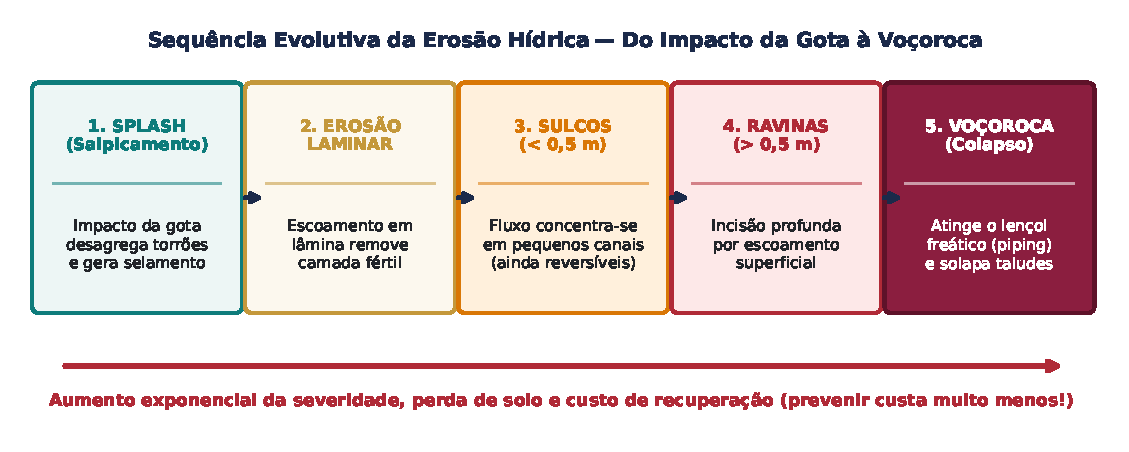
\includegraphics[width=0.94\textwidth]{figures/fig10_evolucao_erosao_linear.pdf}
  \caption{Sequência evolutiva dos processos erosivos hídricos, do impacto da gota (\textit{splash}) ao colapso por voçorocamento, evidenciando o aumento exponencial da severidade e do custo de recuperação.}
  \label{fig:evolucao_erosao_linear}
\end{figure}

Cada estágio possui diagnóstico morfológico e mecânico próprio:
\begin{enumerate}[leftmargin=1.8em, itemsep=3pt]
  \item \textbf{Impacto da gota (\textit{splash}) e selamento superficial:} quando o solo perde cobertura vegetal e serapilheira, as gotas de chuva atingem diretamente os agregados superficiais, rompendo-os e lançando partículas finas (argila e silte) em suspensão. Essas partículas obstruem os poros superficiais, formando uma crosta delgada (\textbf{selamento superficial}) que reduz drasticamente a taxa de infiltração básica.
  \item \textbf{Erosão laminar (entressulcos):} com a infiltração bloqueada pelo selamento ou pela compactação, a água acumula-se e escoa em lâmina difusa sobre a vertente, removendo silenciosamente a camada mais fértil do horizonte A (matéria orgânica, sementes e nutrientes). Por não abrir grandes cicatrizes visíveis no início, costuma passar despercebida até que aflorem raízes, cascalhos ou horizontes subsuperficiais mais claros.
  \item \textbf{Sulcos erosivos ($< 0{,}5\text{ m}$ de profundidade):} irregularidades microtopográficas, marcas de pneus ou linhas de plantio morro abaixo concentram a lâmina d'água em filetes de maior velocidade e tensão cisalhante. Os canais rasos assim abertos são denominados sulcos e, em geral, ainda podem ser corrigidos por práticas conservacionistas e manejo superficial do solo.
  \item \textbf{Ravinas ($> 0{,}5\text{ m}$ de profundidade, sem atingir o lençol freático):} se o escoamento superficial concentrado não for dissipado, os sulcos aprofundam-se e alargam-se, tornando-se incisões permanentes que não são eliminadas por preparo comum do solo. O agente dominante na ravina ainda é o \textbf{escoamento superficial concentrado}, que excava o leito e expande o canal remontantemente (de jusante para montante).
  \item \textbf{Voçorocas (estágio de colapso integrado):} representam a forma mais avançada e destrutiva da erosão linear. Diferenciam-se das ravinas não apenas pelas dimensões métricas, mas sobretudo pelo \textbf{processo hidrogeomorfológico}: a incisão atinge o \textbf{lençol freático} (ou zonas de fluxo subsuperficial saturado). Passam então a atuar simultaneamente o escoamento superficial, a erosão subsuperficial em túneis (\textbf{\textit{piping}}) e a exfiltração na base das paredes, provocando \textbf{solapamento} e escorregamentos sucessivos dos taludes laterais e da cabeceira, mesmo em períodos sem chuva intensa.
\end{enumerate}

\begin{figure}[H]
  \centering
  \begin{minipage}[t]{0.48\textwidth}
    \centering
    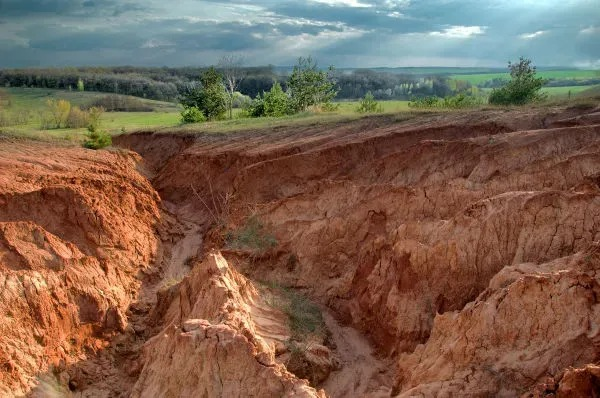
\includegraphics[width=\textwidth,height=4.3cm,keepaspectratio]{figures/foto_vocoroca_severa.jpg}
    \par\small\textbf{(A)} Voçoroca profunda com exposição de horizontes subsuperficiais.
  \end{minipage}\hfill
  \begin{minipage}[t]{0.48\textwidth}
    \centering
    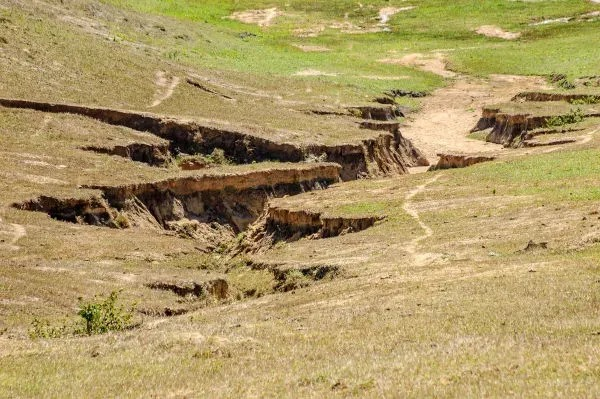
\includegraphics[width=\textwidth,height=4.3cm,keepaspectratio]{figures/foto_pastagem_ravinas.jpg}
    \par\small\textbf{(B)} Cabeceiras erosivas escalonadas em pastagem degradada.
  \end{minipage}
  \caption{\textbf{Registros empíricos de erosão linear severa em vertentes degradadas.} \textit{O que observar:} no painel A, a incisão profunda expõe o perfil pedológico e promove o desmoronamento das paredes laterais por solapamento. No painel B, o avanço regressivo das cabeceiras fragmenta a encosta e intensifica a conectividade de sedimentos para o fundo de vale. Fonte: Acervo didático CHF662.}
  \label{fig:fotos_erosao_linear}
\end{figure}


\section{Instabilidade de Margens Fluviais, Degradação Ripária e Assoreamento}

Na escala da bacia hidrográfica, a erosão das vertentes articula-se diretamente à dinâmica dos canais fluviais e das Áreas de Preservação Permanente (APPs) marginais:
\begin{itemize}[leftmargin=1.5em, itemsep=2.5pt]
  \item \textbf{Degradação ripária e colapso de margens:} a supressão da mata ciliar elimina a malha radicular que confere coesão mecânica aos barrancos (tema aprofundado na bioengenharia do Capítulo 13) e expõe a margem ao impacto direto da corrente fluvial. A erosão na base do talude marginal (\textit{undercutting}) gera quedas em bloco e alargamento desordenado da calha.
  \item \textbf{Assoreamento de canais, açudes e reservatórios:} quando o aporte de sedimentos oriundo das vertentes e margens excede a capacidade de transporte do curso d'água, ocorre deposição no leito. No Semiárido Baiano, o assoreamento reduz rapidamente o volume útil de açudes, barreiros e pequenos barramentos comunitários, agrava a vulnerabilidade hídrica nas estiagens e eleva a turbidez da água.
\end{itemize}

\section{Equação Universal de Perda de Solo (USLE)}

Desenvolvida por Wischmeier e Smith (1978) a partir de milhares de parcelas experimentais e amplamente calibrada para condições tropicais e brasileiras, a \textbf{Equação Universal de Perda de Solo (USLE)} estima a perda média anual de solo por erosão laminar e em sulcos a partir do produto de seis fatores físicos e de manejo.

\begin{boxFormula}[Equação Universal de Perda de Solo (USLE) e Conversão para Rebaixamento]
\[
A = R \cdot K \cdot L \cdot S \cdot C \cdot P
\]
\begin{itemize}[leftmargin=1.4em, itemsep=2pt]
  \item $A$: perda média anual estimada de solo ($\text{t}\cdot\text{ha}^{-1}\cdot\text{ano}^{-1}$).
  \item $R$: fator de \textbf{erosividade da chuva} ($\text{MJ}\cdot\text{mm}\cdot\text{ha}^{-1}\cdot\text{h}^{-1}\cdot\text{ano}^{-1}$); expressa a energia cinética e intensidade máxima das precipitações ao longo do ano.
  \item $K$: fator de \textbf{erodibilidade do solo} ($\text{t}\cdot\text{ha}\cdot\text{h}\cdot\text{ha}^{-1}\cdot\text{MJ}^{-1}\cdot\text{mm}^{-1}$); reflete a suscetibilidade intrínseca do solo à erosão (textura, matéria orgânica, estrutura e permeabilidade).
  \item $L$ e $S$: fatores topográficos de \textbf{comprimento de rampa ($L$)} e \textbf{declividade ($S$)} (adimensionais, frequentemente agrupados como fator $LS$). Quanto maior e mais íngreme a vertente, maior o valor de $LS$.
  \item $C$: fator de \textbf{uso, manejo e cobertura vegetal} (adimensional, entre $\approx 0{,}001$ em floresta densa e $1{,}00$ em solo continuamente descoberto e mobilizado).
  \item $P$: fator de \textbf{práticas conservacionistas} (adimensional, de $1{,}00$ em plantio morro abaixo até $\approx 0{,}50$ em plantio em contorno ou $0{,}20$--$0{,}40$ com terraceamento e cordões vegetados).
\end{itemize}

\textbf{Relação entre Perda de Massa ($A$) e Rebaixamento Superficial ($h$):}
Como $1\text{ ha} = 10.000\text{ m}^2$, uma lâmina de $1\text{ mm}$ ($0{,}001\text{ m}$) de solo em $1\text{ ha}$ possui volume de $10\text{ m}^3$. Multiplicando pela densidade do solo ($D_s$ em $\text{t}\cdot\text{m}^{-3} = \text{g}\cdot\text{cm}^{-3}$), cada $1\text{ mm}$ corresponde a $10 \cdot D_s$ toneladas por hectare:
\[
h\,(\text{mm}\cdot\text{ano}^{-1}) = \frac{A\,(\text{t}\cdot\text{ha}^{-1}\cdot\text{ano}^{-1})}{10 \cdot D_s} \qquad \Longleftrightarrow \qquad A = 10 \cdot D_s \cdot h
\]
\end{boxFormula}

É fundamental destacar duas características essenciais da USLE: (1) o produto $R \cdot K \cdot L \cdot S$ representa o \textbf{potencial natural de erosão} (o solo completamente descoberto e sem práticas conservacionistas); e (2) os fatores $C$ e $P$ são os elementos sobre os quais a gestão territorial e o manejo atuam diretamente, podendo reduzir as perdas em mais de $95\%$, conforme ilustrado na Figura~\ref{fig:usle_sensibilidade}. Além disso, a USLE \textbf{não modela erosão em ravinas profundas, voçorocas ou margens fluviais}, nem quantifica diretamente a deposição na base da vertente. Para estimar o sedimento que chega a um reservatório, associa-se a USLE à Razão de Aporte de Sedimentos ($SDR$).

\begin{figure}[H]
  \centering
  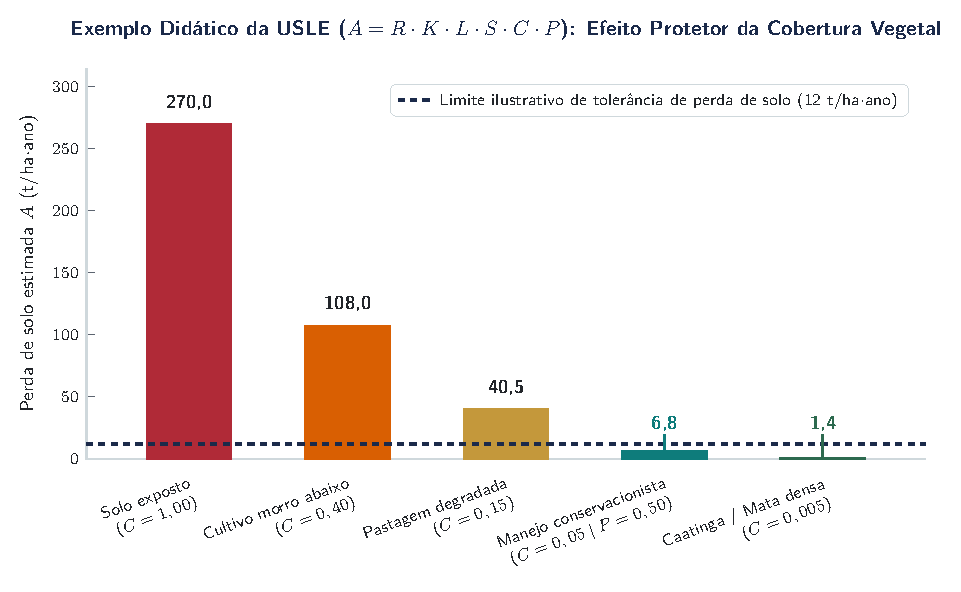
\includegraphics[width=0.88\textwidth]{figures/fig11_usle_sensibilidade.pdf}
  \caption{Análise de sensibilidade da Equação Universal de Perda de Solo ($R = 6.000$, $K = 0{,}03$, $LS = 1{,}5$, potencial natural de $270\text{ t}\cdot\text{ha}^{-1}\cdot\text{ano}^{-1}$) sob cinco cenários de cobertura e manejo frente ao limite ilustrativo de tolerância ($12\text{ t}\cdot\text{ha}^{-1}\cdot\text{ano}^{-1}$).}
  \label{fig:usle_sensibilidade}
\end{figure}

\section{Protocolos Quantitativos de Diagnóstico e Monitoramento em Campo}

Modelos como a USLE fornecem estimativas de planejamento, mas o diagnóstico rigoroso de processos ativos em campo requer medições diretas e rastreáveis:
\begin{enumerate}[leftmargin=1.8em, itemsep=2.5pt]
  \item \textbf{Método dos Pinos de Erosão:} consiste na cravação vertical de vergalhões metálicos ou pinos rígidos (tipicamente de $30$ a $50\text{ cm}$ de comprimento) dispostos em malha ou transectos ao longo da vertente ou talude, deixando uma altura inicial exposta padronizada (ex.: $150\text{ mm}$) marcada com anilha ou pintura. Após cada evento chuvoso ou ciclo anual, mede-se novamente a altura exposta com paquímetro ou régua milimetrada: aumento na altura exposta ($\Delta h > 0$) registra \textbf{rebaixamento erosivo}; diminuição ($\Delta h < 0$) indica \textbf{deposição local de sedimentos}.
  \item \textbf{Estacas de Monitoramento de Recuo de Cabeceira e Bordas:} em ravinas e voçorocas ativas, instalam-se estacas fixas externas a distâncias conhecidas (ex.: $2{,}0$ a $5{,}0\text{ m}$ além da borda instável) em alinhamentos radiais. Medições periódicas da distância entre cada estaca e a borda do talude permitem calcular a taxa de avanço remontante ($\text{m}\cdot\text{ano}^{-1}$).
  \item \textbf{Perfis Transversais de Ravinas e Voçorocas:} em seções fixas espaçadas regularmente pela distância $L_{\text{seg}}$ ao longo do canal erosivo, mede-se a largura superior ($B$), a largura de fundo ($b$) e a profundidade vertical média ($h_{\text{rav}}$) a partir de uma linha de referência nivelada (trena esticada entre estacas), estimando a área da seção trapezoidal por $A = \frac{B + b}{2}\cdot h_{\text{rav}}$. Integrando as áreas transversais ($A_1, A_2, \dots$) pelo método da média das áreas, obtém-se o volume de solo mobilizado ($V = \frac{A_1 + A_2}{2}\cdot L_{\text{seg}}$) e sua massa ($M = V \cdot D_s$).
  \item \textbf{Fichas Padronizadas de Avaliação Visual:} complementam as medições métricas registrando coordenadas geográficas, posição na vertente, cobertura vegetal estimada, presença de selamento, exfiltração subsuperficial (surgências na parede da voçoroca), conectividade com cursos d'água e registro fotográfico com escala métrica.
\end{enumerate}

\etapa{4}{Estudos de Caso e Exemplos Resolvidos Passo a Passo}

\begin{boxExemplo}{12.1 (Básico)}{Aplicação da USLE e Comparação de Cenários de Manejo (Figura~\ref{fig:usle_sensibilidade})}
\passoEnunciado{Uma vertente no Semiárido Baiano apresenta os seguintes fatores físicos naturais: erosividade da chuva $R = 6.000\text{ MJ}\cdot\text{mm}\cdot\text{ha}^{-1}\cdot\text{h}^{-1}\cdot\text{ano}^{-1}$, erodibilidade do solo $K = 0{,}03\text{ t}\cdot\text{ha}\cdot\text{h}\cdot\text{ha}^{-1}\cdot\text{MJ}^{-1}\cdot\text{mm}^{-1}$ e fator topográfico combinado $LS = 1{,}5$. O limite ilustrativo de tolerância de perda de solo adotado para o local é $T = 12{,}0\text{ t}\cdot\text{ha}^{-1}\cdot\text{ano}^{-1}$.}
\passoDados{Cinco cenários de uso e manejo: (1) solo exposto ($C = 1{,}00$; $P = 1{,}00$); (2) cultivo morro abaixo ($C = 0{,}40$; $P = 1{,}00$); (3) pastagem degradada ($C = 0{,}15$; $P = 1{,}00$); (4) manejo conservacionista em contorno ($C = 0{,}05$; $P = 0{,}50$); e (5) Caatinga densa preservada ($C = 0{,}005$; $P = 1{,}00$).}
\passoPedido{Calcular a perda anual estimada ($A$) em cada cenário, verificar quais atendem ao limite de tolerância ($A \le 12{,}0$) e calcular a redução percentual promovida pelo manejo conservacionista em relação ao cultivo morro abaixo.}
\passoMetodo{Cálculo prévio do potencial natural de erosão ($PNE = R \cdot K \cdot LS$) seguido da multiplicação pelos fatores $C$ e $P$ de cada cenário.}
\passoContas{
\textbf{Etapa 1, Potencial Natural de Erosão ($PNE$):}
\[
PNE = R \cdot K \cdot LS = 6.000 \times 0{,}03 \times 1{,}5 = 180 \times 1{,}5 = 270{,}0\text{ t}\cdot\text{ha}^{-1}\cdot\text{ano}^{-1}
\]
Note que as unidades de $\text{MJ}$, $\text{mm}$, $\text{h}$ e um fator $\text{ha}$ cancelam-se rigorosamente entre $R$ e $K$, restando $\text{t}\cdot\text{ha}^{-1}\cdot\text{ano}^{-1}$.

\textbf{Etapa 2, Perda de solo ($A$) nos cinco cenários:}
\begin{align*}
  A_1\; (\text{solo exposto}) &= 270{,}0 \times 1{,}00 \times 1{,}00 = 270{,}0\text{ t}\cdot\text{ha}^{-1}\cdot\text{ano}^{-1} \quad (> 12\text{, crítico}) \\
  A_2\; (\text{cultivo morro abaixo}) &= 270{,}0 \times 0{,}40 \times 1{,}00 = 108{,}0\text{ t}\cdot\text{ha}^{-1}\cdot\text{ano}^{-1} \quad (> 12\text{, insustentável}) \\
  A_3\; (\text{pastagem degradada}) &= 270{,}0 \times 0{,}15 \times 1{,}00 = 40{,}5\text{ t}\cdot\text{ha}^{-1}\cdot\text{ano}^{-1} \quad (> 12\text{, acima do limite}) \\
  A_4\; (\text{manejo conservacionista}) &= 270{,}0 \times 0{,}05 \times 0{,}50 = 6{,}75\text{ t}\cdot\text{ha}^{-1}\cdot\text{ano}^{-1} \quad (\le 12\text{, sustentável}) \\
  A_5\; (\text{Caatinga densa}) &= 270{,}0 \times 0{,}005 \times 1{,}00 = 1{,}35\text{ t}\cdot\text{ha}^{-1}\cdot\text{ano}^{-1} \quad (\le 12\text{, referência})
\end{align*}
\textbf{Etapa 3, Redução do manejo conservacionista ($A_4$) frente ao cultivo morro abaixo ($A_2$):}
\[
\text{Redução} = \frac{108{,}0 - 6{,}75}{108{,}0}\times 100\% = \frac{101{,}25}{108{,}0}\times 100\% = 93{,}75\%
\]}
\passoResposta{Perdas: $270{,}0$ (solo exposto), $108{,}0$ (morro abaixo), $40{,}5$ (pastagem degradada), $6{,}75$ (manejo conservacionista) e $1{,}35\text{ t}\cdot\text{ha}^{-1}\cdot\text{ano}^{-1}$ (Caatinga). Apenas os cenários 4 e 5 atendem ao limite $T = 12\text{ t}\cdot\text{ha}^{-1}\cdot\text{ano}^{-1}$; o manejo conservacionista reduz a erosão em $93{,}75\%$.}
\passoVerificacao{Os valores coincidem integralmente com as barras da Figura~\ref{fig:usle_sensibilidade} (onde $6{,}75$ e $1{,}35$ aparecem arredondados para uma casa decimal: $6{,}8$ e $1{,}4$) e demonstram que a cobertura do solo ($C$) exerce impacto decisivo no controle da erosão.}
\end{boxExemplo}

\begin{boxExemplo}{12.2 (Intermediário)}{Conversão de Perda de Solo (USLE) em Espessura de Rebaixamento Superficial}
\passoEnunciado{Para comunicar a agricultores e gestores o significado físico da perda de solo obtida no cenário de cultivo morro abaixo do Exemplo~12.1 ($A = 108{,}0\text{ t}\cdot\text{ha}^{-1}\cdot\text{ano}^{-1}$), converta essa taxa em espessura anual de solo removido e estime quanto do horizonte A será perdido em $25$ anos.}
\passoDados{$A = 108{,}0\text{ t}\cdot\text{ha}^{-1}\cdot\text{ano}^{-1}$; densidade do solo da camada superficial $D_s = 1{,}35\text{ g}\cdot\text{cm}^{-3} = 1{,}35\text{ t}\cdot\text{m}^{-3}$; horizonte temporal de análise $= 25\text{ anos}$.}
\passoPedido{Calcular a taxa anual de rebaixamento $h$ ($\text{mm}\cdot\text{ano}^{-1}$) e a espessura acumulada removida em $25$ anos (em $\text{cm}$).}
\passoMetodo{Aplicação da relação geométrica $h = A / (10 \cdot D_s)$ e multiplicação pelo horizonte de $25$ anos.}
\passoContas{
\textbf{Etapa 1, Massa correspondente a $1\text{ mm}$ de solo em $1\text{ ha}$:}
\[
M_{1\text{mm}} = 10 \cdot D_s = 10 \times 1{,}35 = 13{,}5\text{ t}\cdot\text{ha}^{-1}\cdot\text{mm}^{-1}
\]
\textbf{Etapa 2, Rebaixamento anual:}
\[
h = \frac{108{,}0}{13{,}5} = 8{,}00\text{ mm}\cdot\text{ano}^{-1}
\]
\textbf{Etapa 3, Rebaixamento acumulado em $25$ anos:}
\[
H_{25} = 8{,}00\text{ mm}\cdot\text{ano}^{-1} \times 25\text{ anos} = 200{,}0\text{ mm} = 20{,}0\text{ cm}
\]}
\passoResposta{Taxa de rebaixamento de $8{,}00\text{ mm}\cdot\text{ano}^{-1}$, removendo $20{,}0\text{ cm}$ de solo superficial em apenas $25$ anos.}
\passoVerificacao{Em solos rasos do Semiárido Baiano (como Neossolos Litólicos e Luvissolos com horizonte A entre $15$ e $25\text{ cm}$), perder $20\text{ cm}$ em um quarto de século significa eliminar completamente a camada biologicamente ativa e expor o horizonte B ou a rocha alterada, processo clássico de desertificação edáfica.}
\end{boxExemplo}

\begin{boxExemplo}{12.3 (Intermediário)}{Monitoramento de Talude pelo Método dos Pinos de Erosão}
\passoEnunciado{Cinco pinos de erosão foram instalados ao longo de um perfil de talude exposto próximo à estrada de acesso de um empreendimento, todos com altura inicial exposta padronizada de $150\text{ mm}$. Após um ciclo hidrológico de $12$ meses, novas leituras foram coletadas com paquímetro.}
\passoDados{Altura inicial exposta em todos os pinos: $h_0 = 150\text{ mm}$. Leituras após $12$ meses (do topo à base do talude): Pino 1 $= 168\text{ mm}$; Pino 2 $= 174\text{ mm}$; Pino 3 $= 162\text{ mm}$; Pino 4 $= 156\text{ mm}$; Pino 5 (sopé do talude) $= 140\text{ mm}$. Densidade do solo local: $D_s = 1{,}40\text{ g}\cdot\text{cm}^{-3}$.}
\passoPedido{Calcular a variação $\Delta h_i$ em cada pino, o balanço líquido médio de rebaixamento ($\Delta \bar{h}$) e a perda líquida equivalente de solo em $\text{t}\cdot\text{ha}^{-1}\cdot\text{ano}^{-1}$.}
\passoMetodo{Cálculo individual $\Delta h_i = h_{1,i} - h_0$ (respeitando sinais positivos para erosão e negativos para deposição), média aritmética e conversão via $A = 10 \cdot D_s \cdot \Delta \bar{h}$.}
\passoContas{
\textbf{Etapa 1, Variação em cada pino:}
\begin{align*}
  \Delta h_1 &= 168 - 150 = +18\text{ mm} \quad (\text{erosão}) \\
  \Delta h_2 &= 174 - 150 = +24\text{ mm} \quad (\text{erosão máxima no terço médio}) \\
  \Delta h_3 &= 162 - 150 = +12\text{ mm} \quad (\text{erosão}) \\
  \Delta h_4 &= 156 - 150 = +6\text{ mm} \quad (\text{erosão moderada}) \\
  \Delta h_5 &= 140 - 150 = -10\text{ mm} \quad (\text{deposição no sopé})
\end{align*}
\textbf{Etapa 2, Balanço líquido médio ($\Delta \bar{h}$):}
\[
\Delta \bar{h} = \frac{18 + 24 + 12 + 6 + (-10)}{5} = \frac{50}{5} = +10{,}0\text{ mm}\cdot\text{ano}^{-1}
\]
\textbf{Etapa 3, Perda líquida equivalente de solo:}
\[
A_{\text{pinos}} = 10 \times 1{,}40 \times 10{,}0 = 140{,}0\text{ t}\cdot\text{ha}^{-1}\cdot\text{ano}^{-1}
\]}
\passoResposta{Rebaixamento líquido médio de $10{,}0\text{ mm}\cdot\text{ano}^{-1}$, correspondente a uma perda líquida equivalente de $140{,}0\text{ t}\cdot\text{ha}^{-1}\cdot\text{ano}^{-1}$.}
\passoVerificacao{O sinal negativo no Pino 5 ($-10\text{ mm}$) é fisicamente esperado em encostas: parte do sedimento removido dos segmentos superiores e médios deposita-se no sopé com a redução da declividade. Desconsiderar o sinal negativo superestimaria o balanço líquido da encosta.}
\end{boxExemplo}

\begin{boxExemplo}{12.4 (Avançado)}{Cubagem de Solo Mobilizado em Ravina por Perfis Transversais}
\passoEnunciado{Para dimensionar estruturas de contenção em uma ravina ativa com $40{,}0\text{ m}$ de extensão, uma equipe levantou duas seções transversais representativas (Seção 1 a montante e Seção 2 a jusante), ambas aproximadas por geometria trapezoidal.}
\passoDados{Comprimento do trecho entre seções: $L = 40{,}0\text{ m}$. Seção 1: largura de topo $B_1 = 3{,}2\text{ m}$, largura de fundo $b_1 = 1{,}2\text{ m}$, profundidade $h_1 = 1{,}5\text{ m}$. Seção 2: $B_2 = 4{,}0\text{ m}$, $b_2 = 1{,}6\text{ m}$, profundidade $h_2 = 2{,}0\text{ m}$. Densidade média do solo do perfil: $D_s = 1{,}45\text{ t}\cdot\text{m}^{-3}$.}
\passoPedido{Calcular a área de cada seção ($A_1$ e $A_2$), o volume total de solo escavado ($V$) pelo método da média das áreas e a massa total mobilizada ($M$).}
\passoMetodo{Área do trapézio $A = \frac{B + b}{2}\cdot h$, volume prismoidal simplificado $V = \frac{A_1 + A_2}{2}\cdot L$ e conversão para massa $M = V \cdot D_s$.}
\passoContas{
\textbf{Etapa 1, Área das seções transversais:}
\[
A_1 = \frac{3{,}2 + 1{,}2}{2}\times 1{,}5 = \frac{4{,}4}{2}\times 1{,}5 = 2{,}2 \times 1{,}5 = 3{,}30\text{ m}^2
\]
\[
A_2 = \frac{4{,}0 + 1{,}6}{2}\times 2{,}0 = \frac{5{,}6}{2}\times 2{,}0 = 2{,}8 \times 2{,}0 = 5{,}60\text{ m}^2
\]
\textbf{Etapa 2, Volume total mobilizado no trecho de $40\text{ m}$:}
\[
V = \frac{3{,}30 + 5{,}60}{2}\times 40{,}0 = \frac{8{,}90}{2}\times 40{,}0 = 4{,}45 \times 40{,}0 = 178{,}0\text{ m}^3
\]
\textbf{Etapa 3, Massa total de solo mobilizada:}
\[
M = 178{,}0\text{ m}^3 \times 1{,}45\text{ t}\cdot\text{m}^{-3} = 258{,}1\text{ t}
\]}
\passoResposta{$A_1 = 3{,}30\text{ m}^2$, $A_2 = 5{,}60\text{ m}^2$, volume escavado $V = 178{,}0\text{ m}^3$ e massa mobilizada de $258{,}1\text{ toneladas}$ de solo.}
\passoVerificacao{Para visualizar a magnitude do impacto, $178\text{ m}^3$ equivalem a aproximadamente $15$ a $18$ caminhões basculantes convencionais carregados de solo removidos de uma única ravina de $40\text{ m}$, grande parte dos quais segue diretamente para drenagens e açudes a jusante.}
\end{boxExemplo}

\begin{boxExemplo}{12.5 (Avançado)}{Estimativa de Assoreamento de Reservatório por USLE e Razão de Aporte ($SDR$)}
\passoEnunciado{Uma microbacia rural de $250\text{ ha}$ no Semiárido Baiano drena para um açude comunitário com capacidade inicial de armazenamento de $160.000\text{ m}^3$. Estudos anteriores estimaram perda média de solo pela USLE de $A = 32{,}0\text{ t}\cdot\text{ha}^{-1}\cdot\text{ano}^{-1}$ na microbacia e Razão de Aporte de Sedimentos $SDR = 0{,}25$ (isto é, $25\%$ do solo erodido nas vertentes atinge o reservatório).}
\passoDados{Área da microbacia: $250\text{ ha}$; perda média USLE: $A = 32{,}0\text{ t}\cdot\text{ha}^{-1}\cdot\text{ano}^{-1}$; $SDR = 0{,}25$; densidade aparente do sedimento depositado no fundo do açude: $\rho_{\text{sed}} = 1{,}25\text{ t}\cdot\text{m}^{-3}$; capacidade útil inicial: $V_0 = 160.000\text{ m}^3$.}
\passoPedido{Calcular (a) a produção anual de sedimentos que chega ao açude ($Y$, em $\text{t}\cdot\text{ano}^{-1}$); (b) o volume assoreado por ano ($V_{\text{sed}}$); e (c) o percentual da capacidade inicial perdido em $20$ anos caso não haja conservação na microbacia.}
\passoMetodo{Cálculo do aporte de sedimentos $Y = A \cdot \text{Área} \cdot SDR$, conversão para volume ($V_{\text{sed}} = Y / \rho_{\text{sed}}$) e projeção linear de $20$ anos frente ao volume inicial.}
\passoContas{
\textbf{Etapa 1, Aporte anual de sedimentos no reservatório ($Y$):}
\[
Y = 32{,}0\text{ t}\cdot\text{ha}^{-1}\cdot\text{ano}^{-1} \times 250\text{ ha} \times 0{,}25 = 8.000 \times 0{,}25 = 2.000{,}0\text{ t}\cdot\text{ano}^{-1}
\]
\textbf{Etapa 2, Volume anual de assoreamento ($V_{\text{sed}}$):}
\[
V_{\text{sed}} = \frac{2.000{,}0\text{ t}\cdot\text{ano}^{-1}}{1{,}25\text{ t}\cdot\text{m}^{-3}} = 1.600{,}0\text{ m}^3\cdot\text{ano}^{-1}
\]
\textbf{Etapa 3, Volume assoreado em $20$ anos e perda percentual de capacidade:}
\[
V_{20} = 1.600{,}0 \times 20 = 32.000{,}0\text{ m}^3
\]
\[
\text{Perda percentual} = \frac{32.000{,}0}{160.000{,}0}\times 100\% = 20{,}0\%
\]}
\passoResposta{Aporte anual de $2.000{,}0\text{ t}\cdot\text{ano}^{-1}$ ($1.600{,}0\text{ m}^3\cdot\text{ano}^{-1}$), provocando perda de $20{,}0\%$ da capacidade de armazenamento do açude em $20$ anos.}
\passoVerificacao{O resultado demonstra a conexão indissociável entre manejo de solos nas vertentes e segurança hídrica no Semiárido: sem controle erosivo na microbacia (redução de $C$ e $P$ e recomposição ripária), um quinto do volume do reservatório desaparece em duas décadas.}
\end{boxExemplo}

\etapa{5}{Erros Mais Comuns e Como Evitá-los}

\begin{boxErro}[Erro 1: Chamar Qualquer Canal Erosivo Profundo de Voçoroca]
\textbf{Equívoco frequente:} Classificar qualquer incisão com mais de $1\text{ m}$ de profundidade automaticamente como voçoroca sem investigar a presença de água subsuperficial.\par
\textbf{Correção técnica:} A distinção geomorfológica entre \textbf{ravina} e \textbf{voçoroca} baseia-se no mecanismo dominante: ravinas são escavadas exclusivamente por escoamento superficial concentrado; voçorocas interceptam o lençol freático ou fluxos subsuperficiais concentrados, apresentando \textit{piping}, surgências de água e solapamento de taludes. Esse diagnóstico muda radicalmente o projeto de recuperação (voçorocas exigem drenagem subsuperficial além do desvio de águas superficiais).
\end{boxErro}

\begin{boxErro}[Erro 2: Aplicar a USLE para Estimar Erosão em Voçorocas ou Margens Fluviais]
\textbf{Equívoco frequente:} Usar $A = R \cdot K \cdot L \cdot S \cdot C \cdot P$ como se o resultado englobasse toda a produção de sedimentos de uma bacia com voçorocas ativas e desmoronamento de margens.\par
\textbf{Correção técnica:} A USLE foi calibrada exclusivamente para \textbf{erosão laminar e em sulcos} nas vertentes. Processos lineares profundos (ravinas e voçorocas) e erosão marginal devem ser quantificados separadamente por perfis transversais, estacas de recuo, levantamento topográfico ou fotogrametria com drone.
\end{boxErro}

\begin{boxErro}[Erro 3: Misturar Unidades Métricas e Inglesas nos Fatores $R$ e $K$ da USLE]
\textbf{Equívoco frequente:} Multiplicar um fator $R$ no Sistema Internacional ($\text{MJ}\cdot\text{mm}\cdot\text{ha}^{-1}\cdot\text{h}^{-1}\cdot\text{ano}^{-1}$) por um fator $K$ retirado de tabelas antigas em unidades norte-americanas sem conversão.\par
\textbf{Correção técnica:} Confira sempre a análise dimensional de $R \cdot K$: no Sistema Internacional, o produto $R \cdot K$ deve resultar diretamente em $\text{t}\cdot\text{ha}^{-1}\cdot\text{ano}^{-1}$. Divergências de ordem de grandeza ($10\times$ ou $100\times$) quase sempre denunciam incompatibilidade de unidades entre $R$ e $K$.
\end{boxErro}

\begin{boxErro}[Erro 4: Ignorar Pinos com Valores Negativos (Deposição) no Balanço de Vertente]
\textbf{Equívoco frequente:} Descartar ou tomar em módulo as leituras de pinos parcialmente soterrados na base de uma encosta.\par
\textbf{Correção técnica:} Pinos com $\Delta h < 0$ registram redistribuição interna de sedimentos (deposição). Para estimar o balanço líquido da vertente, preserva-se o sinal algébrico na média; para analisar separadamente a zona de perda máxima, reportam-se ambos os valores (erosão bruta nos segmentos de perda e balanço líquido total).
\end{boxErro}

\etapa{6}{Exercícios de Fixação}

\subsection*{Nível Básico (Processos Erosivos, Morfologia e Conceitos)}

\begin{enumerate}[leftmargin=1.8em, itemsep=6pt]
  \item Descreva o papel do \textbf{impacto da gota de chuva (\textit{splash})} na formação do selamento superficial e explique como esse fenômeno acelera o surgimento da erosão laminar.
  \espacoResolucao[1.8cm]

  \item Estabeleça a diferença técnica entre \textbf{sulco}, \textbf{ravina} e \textbf{voçoroca} quanto aos processos hidrológicos atuantes e à reversibilidade por manejo convencional.
  \espacoResolucao[1.8cm]

  \item O que é \textbf{\textit{piping}} e por que sua identificação em campo é decisiva antes de propor obras de estabilização em uma encosta?
  \espacoResolucao[1.8cm]

  \item Explique o significado físico de cada um dos seis fatores da Equação Universal de Perda de Solo ($A = R \cdot K \cdot L \cdot S \cdot C \cdot P$) e indique quais dois fatores podem ser diretamente modificados pelo manejo conservacionista.
  \espacoResolucao[1.8cm]

  \item Explique como a degradação de áreas ripárias (matas ciliares) contribui simultaneamente para a instabilidade de margens fluviais e para o assoreamento de reservatórios.
  \espacoResolucao[1.8cm]
\end{enumerate}

\subsection*{Nível Intermediário (Cálculos de USLE, Pinos, Perfis e Assoreamento)}

\begin{enumerate}[leftmargin=1.8em, itemsep=6pt, resume]
  \item Uma área agrícola apresenta $R = 5.000\text{ MJ}\cdot\text{mm}\cdot\text{ha}^{-1}\cdot\text{h}^{-1}\cdot\text{ano}^{-1}$, $K = 0{,}025\text{ t}\cdot\text{ha}\cdot\text{h}\cdot\text{ha}^{-1}\cdot\text{MJ}^{-1}\cdot\text{mm}^{-1}$, $LS = 2{,}0$ e fator de manejo $C = 0{,}20$. Calcule a perda anual de solo ($A$) sob plantio morro abaixo ($P = 1{,}00$) e sob plantio em contorno ($P = 0{,}50$).
  \espacoResolucao[2.2cm]

  \item Uma vertente submetida a uso intensivo registra perda anual estimada de $A = 70{,}0\text{ t}\cdot\text{ha}^{-1}\cdot\text{ano}^{-1}$ em um solo com densidade $D_s = 1{,}40\text{ g}\cdot\text{cm}^{-3}$. Calcule o rebaixamento anual da superfície ($h$, em $\text{mm}\cdot\text{ano}^{-1}$) e a espessura acumulada perdida em $20$ anos (em $\text{cm}$).
  \espacoResolucao[2.2cm]

  \item Quatro pinos de erosão instalados em uma encosta registraram, após um ano, as seguintes variações de altura exposta ($\Delta h$): $+14\text{ mm}$, $+18\text{ mm}$, $+10\text{ mm}$ e $-2\text{ mm}$. Sabendo que a densidade do solo é $D_s = 1{,}30\text{ g}\cdot\text{cm}^{-3}$, calcule o rebaixamento líquido médio ($\Delta \bar{h}$) e a perda líquida equivalente em $\text{t}\cdot\text{ha}^{-1}\cdot\text{ano}^{-1}$.
  \espacoResolucao[2.2cm]

  \item Uma ravina com $30{,}0\text{ m}$ de extensão teve duas seções transversais trapezoidais medidas: Seção 1 ($B_1 = 2{,}4\text{ m}$; $b_1 = 0{,}8\text{ m}$; $h_1 = 1{,}0\text{ m}$) e Seção 2 ($B_2 = 3{,}6\text{ m}$; $b_2 = 1{,}2\text{ m}$; $h_2 = 1{,}5\text{ m}$). Considerando $D_s = 1{,}50\text{ t}\cdot\text{m}^{-3}$, calcule o volume total ($V$) e a massa ($M$) de solo mobilizado.
  \espacoResolucao[2.2cm]

  \item Uma microbacia de $400\text{ ha}$ apresenta perda média de solo $A = 25{,}0\text{ t}\cdot\text{ha}^{-1}\cdot\text{ano}^{-1}$ e $SDR = 0{,}20$, drenando para um açude de $80.000\text{ m}^3$ de capacidade útil inicial. Adotando $\rho_{\text{sed}} = 1{,}25\text{ t}\cdot\text{m}^{-3}$, calcule o volume anual assoreado e o percentual de capacidade perdido em $10$ anos.
  \espacoResolucao[2.2cm]
\end{enumerate}

\subsection*{Nível Aplicado (Questões Objetivas A--E)}

\begin{enumerate}[leftmargin=1.8em, itemsep=6pt, resume]
  \item Na sequência evolutiva da erosão hídrica (Guerra; Cunha, 1996), a transição de uma ravina para uma voçoroca caracteriza-se fundamentalmente por:
  \begin{alternativas}
    \item Interrupção completa do escoamento superficial durante os eventos de chuva.
    \item Interseção da incisão com o lençol freático ou fluxos subsuperficiais concentrados, desencadeando \textit{piping} e solapamento de taludes.
    \item Reversibilidade imediata por uma única operação de aração rasa do solo.
    \item Deposição contínua de matéria orgânica que fecha naturalmente o canal em poucos meses.
    \item Ausência de recuo remontante na cabeceira da feição erosiva.
  \end{alternativas}

  \item A respeito das limitações metodológicas da Equação Universal de Perda de Solo (USLE), assinale a alternativa correta:
  \begin{alternativas}
    \item A USLE quantifica diretamente o volume escavado em grandes voçorocas causadas por \textit{piping}.
    \item O fator $K$ representa a energia cinética das chuvas e depende exclusivamente do regime climático regional.
    \item A USLE estima a perda média anual por erosão laminar e em sulcos nas vertentes, não computando diretamente erosão em voçorocas, margens fluviais nem deposição ao longo do trajeto sem o uso do $SDR$.
    \item A redução do fator $C$ por meio de cobertura vegetal aumenta proporcionalmente a perda de solo $A$.
    \item O produto $C \cdot P$ representa o potencial natural de erosão de uma bacia independente da ação humana.
  \end{alternativas}

  \item Uma parcela experimental apresenta $R = 4.000\text{ MJ}\cdot\text{mm}\cdot\text{ha}^{-1}\cdot\text{h}^{-1}\cdot\text{ano}^{-1}$, $K = 0{,}04\text{ t}\cdot\text{ha}\cdot\text{h}\cdot\text{ha}^{-1}\cdot\text{MJ}^{-1}\cdot\text{mm}^{-1}$, $LS = 1{,}5$, $C = 0{,}10$ e $P = 0{,}50$. A perda média anual de solo ($A$) estimada pela USLE é:
  \begin{alternativas}
    \item $6{,}0\text{ t}\cdot\text{ha}^{-1}\cdot\text{ano}^{-1}$.
    \item $12{,}0\text{ t}\cdot\text{ha}^{-1}\cdot\text{ano}^{-1}$.
    \item $24{,}0\text{ t}\cdot\text{ha}^{-1}\cdot\text{ano}^{-1}$.
    \item $48{,}0\text{ t}\cdot\text{ha}^{-1}\cdot\text{ano}^{-1}$.
    \item $240{,}0\text{ t}\cdot\text{ha}^{-1}\cdot\text{ano}^{-1}$.
  \end{alternativas}

  \item No monitoramento de processos erosivos em campo, o método mais adequado para mensurar a taxa anual de recuo remontante da cabeceira de uma voçoroca ativa é:
  \begin{alternativas}
    \item Determinação de pH e saturação por bases em laboratório.
    \item Instalação de estacas fixas de referência externas à borda instável com medições periódicas de distância até a escarpa.
    \item Uso isolado de infiltrômetro de anel dentro do leito alagado do rio principal.
    \item Cálculo exclusivo do fator $R$ a partir da precipitação média mensal.
    \item Estimativa visual sem marco fixo nem registro de data.
  \end{alternativas}

  \item Em uma parcela monitorada com quatro pinos de erosão durante $12$ meses, as variações de altura exposta foram $+12\text{ mm}$, $+8\text{ mm}$, $+16\text{ mm}$ e $+4\text{ mm}$. Adotando $D_s = 1{,}25\text{ g}\cdot\text{cm}^{-3}$, a perda de solo equivalente no período é:
  \begin{alternativas}
    \item $10{,}0\text{ t}\cdot\text{ha}^{-1}\cdot\text{ano}^{-1}$.
    \item $50{,}0\text{ t}\cdot\text{ha}^{-1}\cdot\text{ano}^{-1}$.
    \item $100{,}0\text{ t}\cdot\text{ha}^{-1}\cdot\text{ano}^{-1}$.
    \item $125{,}0\text{ t}\cdot\text{ha}^{-1}\cdot\text{ano}^{-1}$.
    \item $150{,}0\text{ t}\cdot\text{ha}^{-1}\cdot\text{ano}^{-1}$.
  \end{alternativas}
\end{enumerate}

\etapa{7}{Questões no Estilo ENADE e Concursos Ambientais}

\begin{boxDica}[Integração entre Diagnóstico (Módulo 4) e Intervenção (Módulo 5)]
Em concursos e no ENADE, o diagnóstico da forma erosiva (laminar, sulco, ravina ou voçoroca) aparece quase sempre acoplado à escolha da técnica de controle. Lembre a regra de ouro: prevenir com cobertura ($C$) e conservação ($P$) custa uma fração mínima do custo necessário para estabilizar uma voçoroca instalada.
\end{boxDica}

\begin{enumerate}[leftmargin=1.8em, itemsep=7pt]
  \item \textbf{[Questão Autoral, Estilo ENADE / Geografia]} Durante o diagnóstico ambiental de uma microbacia rural no interior baiano, observou-se uma grande incisão linear com $4{,}2\text{ m}$ de profundidade, paredes subverticais com marcas de escorregamento rotacional, dutos subterrâneos drenando água na base do talude mesmo após $20$ dias sem chuva e forte assoreamento de um riacho a jusante. Com base na geomorfologia da erosão linear, conclui-se que a feição corresponde a:
  \begin{alternativas}
    \item Erosão laminar incipiente, controlável apenas com adubação química superficial.
    \item Sulco raso efêmero, gerado exclusivamente por impacto direto da gota (\textit{splash}).
    \item Ravina rasa desconectada do sistema hidrogeológico local.
    \item Voçoroca ativa com atuação combinada de fluxo superficial, exfiltração do lençol freático, \textit{piping} e solapamento de taludes, demandando drenagem superficial e subsuperficial associada à estabilização de taludes.
    \item Processo natural de equilíbrio ecodinâmico estável segundo Tricart (1977), sem necessidade de intervenção.
  \end{alternativas}

  \item \textbf{[Questão Autoral, Estilo Concurso Analista Ambiental]} Um gestor público dispõe de recursos limitados para reduzir o assoreamento de um açude abastecedor no Semiárido. Simulações com a USLE indicaram que duas sub-bacias possuem igual área e igual clima ($R$), porém a Sub-bacia 1 possui solo exposto ($C = 0{,}80$; $P = 1{,}00$) sobre vertentes íngremes ($LS = 2{,}5$), enquanto a Sub-bacia 2 possui Caatinga conservada ($C = 0{,}01$; $P = 1{,}00$) em relevo suave ($LS = 0{,}5$). Considerando igual erodibilidade $K$, a razão entre a perda de solo estimada na Sub-bacia 1 e na Sub-bacia 2 ($A_1 / A_2$) é igual a:
  \begin{alternativas}
    \item $4$ vezes maior.
    \item $40$ vezes maior.
    \item $80$ vezes maior.
    \item $200$ vezes maior.
    \item $400$ vezes maior.
  \end{alternativas}

  \item \textbf{[Questão Autoral, Estilo Concurso Geógrafo / Órgão Estadual de Meio Ambiente]} Ao elaborar o diagnóstico de áreas degradadas para um Relatório Ambiental, qual combinação de ferramentas garante simultaneamente avaliação da erosão difusa nas vertentes, monitoramento direto de rebaixamento em taludes e quantificação do volume de solo mobilizado em ravinas?
  \begin{alternativas}
    \item Apenas entrevista com moradores locais e consulta à precipitação média anual.
    \item USLE aplicada às vertentes, malha de pinos de erosão em taludes expostos e levantamento de perfis transversais georreferenciados nas ravinas.
    \item Apenas análise química de $V\%$ e pH no fundo do reservatório assoreado.
    \item Cálculo isolado do fator $R$ sem considerar uso da terra nem declividade.
    \item Medição única da densidade de partículas ($D_p$) em laboratório.
  \end{alternativas}
\end{enumerate}

\clearpage
\etapa{8}{Gabarito Comentado do Capítulo 12}

\begin{boxGabarito}[Resoluções Completas: Exercícios de Fixação (1 a 15)]
\begin{enumerate}[leftmargin=1.6em, itemsep=4pt]
  \item O impacto direto das gotas de chuva (\textit{splash}) sobre solo desprotegido desagrega torrões e libera argila e silte em suspensão. Essas partículas finas entopem os poros da superfície, criando uma crosta de baixa permeabilidade (\textbf{selamento superficial}). Com a infiltração drasticamente reduzida, a água acumula-se na superfície e escoa em lâmina difusa, iniciando a erosão laminar.
  \item \textbf{Sulco:} incisão rasa ($<0{,}5\text{ m}$) gerada por concentração inicial do escoamento superficial, ainda reversível por manejo e práticas conservacionistas. \textbf{Ravina:} incisão profunda ($>0{,}5\text{ m}$) permanente, dominada por escoamento superficial concentrado, que não pode ser eliminada por preparo comum. \textbf{Voçoroca:} estágio de colapso em que a incisão atinge o lençol freático ou fluxos subsuperficiais, combinando escoamento superficial, \textit{piping} e solapamento de taludes.
  \item \textbf{\textit{Piping}} é a erosão subsuperficial tubular produzida pelo carreamento interno de partículas finas pela água em percolação concentrada. Sua identificação é crucial porque obras apenas superficiais (sem drenagem profunda adequada) falham quando o solo continua sendo escavado por baixo, causando desabamento das estruturas.
  \item $R$: erosividade da chuva; $K$: erodibilidade intrínseca do solo; $L$: comprimento de rampa; $S$: declividade da vertente; $C$: uso, manejo e cobertura vegetal; $P$: práticas conservacionistas de suporte. Os fatores diretamente modificáveis pelo manejo são \textbf{$C$} (cobertura vegetal, plantio direto, revegetação) e \textbf{$P$} (plantio em contorno, terraceamento, cordões vegetados).
  \item A remoção da vegetação ripária elimina o reforço mecânico das raízes nos barrancos (favorecendo solapamento e queda de margens) e destrói o filtro físico que retinha sedimentos oriundos das vertentes, aumentando a carga sólida transportada até canais e reservatórios (assoreamento).
  \item \textbf{Passo a passo:}
  $PNE = 5.000 \times 0{,}025 \times 2{,}0 = 250{,}0\text{ t}\cdot\text{ha}^{-1}\cdot\text{ano}^{-1}$.
  Morro abaixo ($C = 0{,}20$, $P = 1{,}00$): $A_1 = 250{,}0 \times 0{,}20 \times 1{,}00 = \mathbf{50{,}0\text{ t}\cdot\text{ha}^{-1}\cdot\text{ano}^{-1}}$.
  Em contorno ($C = 0{,}20$, $P = 0{,}50$): $A_2 = 250{,}0 \times 0{,}20 \times 0{,}50 = \mathbf{25{,}0\text{ t}\cdot\text{ha}^{-1}\cdot\text{ano}^{-1}}$.
  \item \textbf{Passo a passo:}
  $h = \frac{A}{10 \cdot D_s} = \frac{70{,}0}{10 \times 1{,}40} = \frac{70{,}0}{14{,}0} = \mathbf{5{,}00\text{ mm}\cdot\text{ano}^{-1}}$.
  Em $20$ anos: $5{,}00 \times 20 = 100{,}0\text{ mm} = \mathbf{10{,}0\text{ cm}}$.
  \item \textbf{Passo a passo:}
  $\Delta \bar{h} = \frac{14 + 18 + 10 + (-2)}{4} = \frac{40}{4} = \mathbf{+10{,}0\text{ mm}\cdot\text{ano}^{-1}}$.
  Perda equivalente: $A = 10 \times 1{,}30 \times 10{,}0 = \mathbf{130{,}0\text{ t}\cdot\text{ha}^{-1}\cdot\text{ano}^{-1}}$.
  \item \textbf{Passo a passo:}
  $A_1 = \frac{2{,}4 + 0{,}8}{2}\times 1{,}0 = 1{,}60\text{ m}^2$.
  $A_2 = \frac{3{,}6 + 1{,}2}{2}\times 1{,}5 = 3{,}60\text{ m}^2$.
  Volume: $V = \frac{1{,}60 + 3{,}60}{2}\times 30{,}0 = 2{,}60 \times 30{,}0 = \mathbf{78{,}0\text{ m}^3}$.
  Massa: $M = 78{,}0 \times 1{,}50 = \mathbf{117{,}0\text{ t}}$.
  \item \textbf{Passo a passo:}
  Aporte anual: $Y = 400 \times 25{,}0 \times 0{,}20 = 2.000{,}0\text{ t}\cdot\text{ano}^{-1}$.
  Volume assoreado anual: $V_{\text{sed}} = 2.000{,}0 / 1{,}25 = \mathbf{1.600{,}0\text{ m}^3\cdot\text{ano}^{-1}}$.
  Em $10$ anos: $16.000{,}0\text{ m}^3$. Perda percentual: $(16.000 / 80.000)\times 100\% = \mathbf{20{,}0\%}$.
  \item \textbf{Gabarito: (B).} O critério geomorfológico central da passagem de ravina para voçoroca é a interseção com o lençol freático ou fluxos subsuperficiais, ativando \textit{piping} e solapamento dos taludes.
  \item \textbf{Gabarito: (C).} A USLE estima erosão laminar e em sulcos nas vertentes; para aportes em bacias, requer $SDR$, e processos lineares profundos ou marginais exigem medições específicas.
  \item \textbf{Gabarito: (B).} $A = 4.000 \times 0{,}04 \times 1{,}5 \times 0{,}10 \times 0{,}50 = 160 \times 1{,}5 \times 0{,}05 = 240 \times 0{,}05 = \mathbf{12{,}0\text{ t}\cdot\text{ha}^{-1}\cdot\text{ano}^{-1}}$.
  \item \textbf{Gabarito: (B).} Estacas fixas externas posicionadas fora da zona de ruptura fornecem referência estável para medir com trena o recuo anual da cabeceira da voçoroca.
  \item \textbf{Gabarito: (D).} Média dos pinos: $(12 + 8 + 16 + 4)/4 = 40/4 = 10{,}0\text{ mm}\cdot\text{ano}^{-1}$. Conversão: $A = 10 \times 1{,}25 \times 10{,}0 = \mathbf{125{,}0\text{ t}\cdot\text{ha}^{-1}\cdot\text{ano}^{-1}}$.
\end{enumerate}
\end{boxGabarito}

\begin{boxGabarito}[Resoluções Completas: Questões ENADE e Concursos (1 a 3)]
\begin{enumerate}[leftmargin=1.6em, itemsep=4pt]
  \item \textbf{Gabarito: (D).} A presença de água emergindo em dutos na base do talude mesmo após $20$ dias sem chuva comprova interceptação do lençol freático e \textit{piping}, definindo inequivocamente uma \textbf{voçoroca ativa}.
  \item \textbf{Gabarito: (E).} Como $R$, $K$ e $P$ são idênticos, a razão simplifica-se para:
  \[
  \frac{A_1}{A_2} = \frac{LS_1 \cdot C_1}{LS_2 \cdot C_2} = \frac{2{,}5 \times 0{,}80}{0{,}5 \times 0{,}01} = \frac{2{,}00}{0{,}005} = \mathbf{400}\text{ vezes maior.}
  \]
  \item \textbf{Gabarito: (B).} Apenas a combinação de USLE (erosão laminar e em sulcos), pinos de erosão (rebaixamento direto em taludes) e perfis transversais (cubagem de ravinas) cobre integralmente os três processos citados.
\end{enumerate}
\end{boxGabarito}

\begin{boxResumo}
\begin{itemize}[leftmargin=1.4em, itemsep=2.5pt]
  \item \textbf{Sequência evolutiva:} \textit{splash} + selamento $\rightarrow$ erosão laminar $\rightarrow$ sulcos ($<0{,}5\text{ m}$) $\rightarrow$ ravinas ($>0{,}5\text{ m}$, fluxo superficial) $\rightarrow$ voçorocas (lençol freático, \textit{piping} e solapamento).
  \item \textbf{USLE ($A = R \cdot K \cdot L \cdot S \cdot C \cdot P$):} separa o potencial natural ($R\cdot K\cdot LS$) do efeito protetor do manejo ($C\cdot P$). Conversão de massa para espessura: $h\,(\text{mm}\cdot\text{ano}^{-1}) = A / (10 \cdot D_s)$.
  \item \textbf{Monitoramento em campo:} pinos de erosão (balanço líquido $\Delta \bar{h}$), estacas externas (recuo de cabeceira), perfis transversais ($V = \frac{A_1+A_2}{2}\cdot L$) e aporte a reservatórios ($Y = A \cdot \text{Área} \cdot SDR$).
\end{itemize}
\end{boxResumo}

\begin{boxTeste}
Responda com \textbf{V} (Verdadeiro) ou \textbf{F} (Falso) e confira abaixo:
\begin{enumerate}[leftmargin=1.6em, itemsep=3pt]
  \item ( \quad ) O selamento superficial causado pelo impacto direto das gotas de chuva (\textit{splash}) reduz a taxa de infiltração e intensifica o escoamento superficial.
  \item ( \quad ) A USLE inclui em seu resultado o volume total de solo escavado por \textit{piping} em voçorocas profundas.
  \item ( \quad ) Em uma malha de pinos de erosão, uma leitura final de altura exposta menor que a leitura inicial ($\Delta h < 0$) indica deposição local de sedimentos.
  \item ( \quad ) Para uma mesma taxa de perda de solo $A = 140\text{ t}\cdot\text{ha}^{-1}\cdot\text{ano}^{-1}$ e densidade $D_s = 1{,}40\text{ g}\cdot\text{cm}^{-3}$, a superfície do terreno sofre rebaixamento médio de $10\text{ mm}\cdot\text{ano}^{-1}$.
\end{enumerate}
\vspace{4pt}
{\footnotesize\textbf{Gabarito do Checkpoint:} 1-\V \quad|\quad 2-\F\ (a USLE modela apenas erosão laminar e em sulcos) \quad|\quad 3-\V \quad|\quad 4-\V\ ($140 / (10 \times 1{,}40) = 10\text{ mm}\cdot\text{ano}^{-1}$).}
\end{boxTeste}

\clearpage
\phantomsection
\addcontentsline{toc}{chapter}{Simulado e Revisão Integrada do Módulo 4}
\chapter*{Simulado e Revisão Integrada: Módulo 4}
\markboth{SIMULADO DO MÓDULO 4}{SIMULADO DO MÓDULO 4}

\noindent\tagCampo\ \tagPratica
\vspace{6pt}

\begin{boxConceito}[Instruções do Simulado Integrado (Capítulos 10, 11 e 12)]
Este simulado integra os conteúdos das Semanas 11 a 13 (Indicadores Ambientais e PEIR no Semiárido Baiano, Qualidade do Solo e Diagnóstico de Erosão Linear/USLE), compondo a base técnica direta do seu Trabalho Prático Final.
\begin{itemize}[leftmargin=1.5em, itemsep=2pt]
  \item \textbf{Tempo sugerido:} $90$ minutos sem consulta ao gabarito.
  \item \textbf{Estrutura:} $8$ questões objetivas autorais no estilo ENADE e concursos ambientais (valor: $0{,}75$ ponto cada $= 6{,}0$ pontos) e $2$ questões dissertativas aplicadas (valor: $2{,}0$ pontos cada $= 4{,}0$ pontos).
  \item Ao concluir, confira o \textbf{Gabarito Comentado}, o \textbf{Espelho Dissertativo} e preencha a \textbf{Tabela de Diagnóstico de Revisão} na página seguinte.
\end{itemize}
\end{boxConceito}

\section*{Parte I: Questões Objetivas (Estilo ENADE e Concursos Ambientais)}

\begin{enumerate}[leftmargin=1.8em, itemsep=8pt]
  \item \textbf{[Cap. 10, Critérios de Indicadores]} Na estruturação de um plano de monitoramento ambiental conforme OECD (2003), Fidalgo (2003) e IBGE (2018), um técnico propôs substituir um protocolo laboratorial de altíssimo custo e baixa periodicidade por medições semestrais padronizadas de cobertura vegetal e densidade de focos erosivos por quilômetro de estrada. Essa substituição fortalece principalmente qual critério de seleção de indicadores?
  \begin{alternativas}
    \item Subjetividade interpretativa.
    \item Mensurabilidade e viabilidade operacional de acompanhamento temporal.
    \item Esteticismo paisagístico.
    \item Independência frente às metas de gestão.
    \item Exclusividade para áreas urbanas impermeabilizadas.
  \end{alternativas}

  \item \textbf{[Cap. 10, Modelo PEIR e Campo no Semiárido]} No diagnóstico integrado de um complexo eólico na região de Canudos (BA), associaram-se corretamente os quatro compartimentos do modelo PEIR. Assinale a alternativa em que há correspondência técnica exata:
  \begin{alternativas}
    \item Pressão: colisão de aves; Estado: PRAD executado; Impacto: velocidade dos ventos alísios; Resposta: supressão vegetal.
    \item Pressão: terraplenagem de platôs e abertura de acessos na Caatinga; Estado: aumento da fração de solo exposto e da densidade do solo; Impacto: erosão linear em taludes e fragmentação de rotas da avifauna; Resposta: drenagem pluvial, bioengenharia e zonas de exclusão para aves ameaçadas.
    \item Pressão: zonas de exclusão para avifauna; Estado: ravinas profundas; Impacto: abertura de acessos; Resposta: solo exposto.
    \item Pressão: chuvas convectivas naturais; Estado: PRAD; Impacto: densidade viária; Resposta: assoreamento de barreiros.
    \item Pressão: geração de energia elétrica; Estado: conflitos fundiários; Impacto: cobertura vegetal nativa; Resposta: terraplenagem de novos platôs.
  \end{alternativas}

  \item \textbf{[Cap. 10, Eixo Energético do Submédio São Francisco]} Em relação ao eixo territorial que compreende Sobradinho, Casa Nova, Sento Sé, Juazeiro, Rodelas e Paulo Afonso, é correto afirmar que:
  \begin{alternativas}
    \item A expansão eólica nessa faixa ocorreu de forma desvinculada da rede de transmissão construída historicamente a partir das usinas hidrelétricas do São Francisco.
    \item Os impactos hidrelétricos restringem-se ao local exato das barragens, sem afetar o pulso natural de cheias, a agricultura de vazante ou os usos múltiplos da água a jusante.
    \item A convivência entre matriz hidrelétrica, parques eólicos, perímetros irrigados e comunidades locais demanda indicadores ambientais integrados que articulem gestão hídrica, conservação da Caatinga e ordenamento territorial.
    \item O bioma predominante nesse eixo é a Floresta Ombrófila Densa, o que impede a ocorrência de déficits hídricos sazonais.
    \item A regularização de vazões elimina todos os conflitos entre geração de energia e agricultura irrigada durante estiagens prolongadas.
  \end{alternativas}

  \item \textbf{[Cap. 11, Física e Química do Solo]} Uma amostra indeformada coletada em anel de $100\text{ cm}^3$ apresentou massa seca de $159\text{ g}$ (adote $D_p = 2{,}65\text{ g}\cdot\text{cm}^{-3}$), e a análise química indicou teor de matéria orgânica $MO = 17{,}24\text{ g}\cdot\text{kg}^{-1}$. Os valores de porosidade total ($P_t$) e de carbono orgânico total ($CO$, pelo fator de van Bemmelen $1{,}724$) são, respectivamente:
  \begin{alternativas}
    \item $30{,}0\%$ e $10{,}0\text{ g}\cdot\text{kg}^{-1}$.
    \item $40{,}0\%$ e $10{,}0\text{ g}\cdot\text{kg}^{-1}$.
    \item $40{,}0\%$ e $29{,}7\text{ g}\cdot\text{kg}^{-1}$.
    \item $60{,}0\%$ e $10{,}0\text{ g}\cdot\text{kg}^{-1}$.
    \item $60{,}0\%$ e $29{,}7\text{ g}\cdot\text{kg}^{-1}$.
  \end{alternativas}

  \item \textbf{[Cap. 11, Normalização e IQS]} Em uma área sob recuperação ambiental, mediram-se quatro indicadores de qualidade do solo comparados a uma referência local:
  \begin{itemize}[leftmargin=1.4em, itemsep=1.5pt]
    \item $MO$ (maior melhor): $24\text{ g}\cdot\text{kg}^{-1}$ (referência: $30\text{ g}\cdot\text{kg}^{-1}$);
    \item $TIB$ (maior melhor): $30\text{ mm}\cdot\text{h}^{-1}$ (referência: $60\text{ mm}\cdot\text{h}^{-1}$);
    \item $D_s$ (menor melhor): $1{,}50\text{ g}\cdot\text{cm}^{-3}$ (referência: $1{,}20\text{ g}\cdot\text{cm}^{-3}$);
    \item $DMP$ de agregados (maior melhor): $1{,}50\text{ mm}$ (referência: $3{,}00\text{ mm}$).
  \end{itemize}
  O Índice de Qualidade do Solo simples ($\text{IQS}_{\text{simples}}$) dessa área é igual a:
  \begin{alternativas}
    \item $0{,}500$.
    \item $0{,}600$.
    \item $0{,}650$.
    \item $0{,}725$.
    \item $0{,}800$.
  \end{alternativas}

  \item \textbf{[Cap. 12, Processos Erosivos Lineares]} Durante vistoria em uma encosta degradada, o geógrafo registrou: (i) crosta superficial fina e impermeabilizada nas áreas de solo nu; (ii) pequenos canais rasos de $0{,}25\text{ m}$ de profundidade ao longo de trilhas; e (iii) no terço inferior, uma grande fenda de $3{,}8\text{ m}$ de profundidade com surgência contínua de água subterrânea e blocos de solo desabando nas paredes. Os três fenômenos observados correspondem, respectivamente, a:
  \begin{alternativas}
    \item \textit{Piping}, voçoroca e erosão laminar.
    \item Selamento superficial, sulcos erosivos e voçoroca ativa.
    \item Assoreamento fluvial, ravina e salpicamento.
    \item Compactação profunda, voçoroca e sulco efêmero.
    \item Selamento superficial, voçoroca e ravina estável.
  \end{alternativas}

  \item \textbf{[Cap. 12, Equação Universal de Perda de Solo]} Uma encosta cultivada possui $R = 5.500\text{ MJ}\cdot\text{mm}\cdot\text{ha}^{-1}\cdot\text{h}^{-1}\cdot\text{ano}^{-1}$, $K = 0{,}02\text{ t}\cdot\text{ha}\cdot\text{h}\cdot\text{ha}^{-1}\cdot\text{MJ}^{-1}\cdot\text{mm}^{-1}$ e $LS = 2{,}0$. Atualmente, sob manejo convencional morro abaixo ($C = 0{,}30$; $P = 1{,}00$), a área sofre forte degradação. Caso seja implantado sistema conservacionista com cobertura permanente e plantio em contorno ($C = 0{,}05$; $P = 0{,}50$), a perda de solo anual passará de:
  \begin{alternativas}
    \item $66{,}0$ para $5{,}5\text{ t}\cdot\text{ha}^{-1}\cdot\text{ano}^{-1}$ (redução de $91{,}67\%$).
    \item $66{,}0$ para $11{,}0\text{ t}\cdot\text{ha}^{-1}\cdot\text{ano}^{-1}$ (redução de $83{,}33\%$).
    \item $110{,}0$ para $5{,}5\text{ t}\cdot\text{ha}^{-1}\cdot\text{ano}^{-1}$ (redução de $95{,}00\%$).
    \item $220{,}0$ para $11{,}0\text{ t}\cdot\text{ha}^{-1}\cdot\text{ano}^{-1}$ (redução de $95{,}00\%$).
    \item $33{,}0$ para $5{,}5\text{ t}\cdot\text{ha}^{-1}\cdot\text{ano}^{-1}$ (redução de $83{,}33\%$).
  \end{alternativas}

  \item \textbf{[Cap. 12, Protocolos de Campo]} Sobre os métodos quantitativos de monitoramento erosivo em campo, assinale a alternativa \textbf{INCORRETA}:
  \begin{alternativas}
    \item No método dos pinos de erosão, o aumento da altura exposta do pino ao longo do tempo indica rebaixamento erosivo do terreno.
    \item Perfis transversais repetidos em seções fixas de uma ravina permitem calcular o volume de solo mobilizado entre campanhas.
    \item Estacas externas posicionadas fora da borda de ruptura permitem monitorar a velocidade de recuo remontante da cabeceira de voçorocas.
    \item O fator $SDR$ (Razão de Aporte de Sedimentos) permite estimar que fração do solo erodido nas vertentes efetivamente chega ao reservatório ou exutório da bacia.
    \item A medição de apenas um pino isolado no topo da encosta dispensa réplicas espaciais e representa com exatidão o balanço de sedimentos de toda a bacia hidrográfica.
  \end{alternativas}
\end{enumerate}

\section*{Parte II: Questões Dissertativas Aplicadas}

\begin{enumerate}[leftmargin=1.8em, itemsep=8pt, start=9]
  \item \textbf{[Integração Caps. 10 e 11, PEIR e Qualidade do Solo no Semiárido]} Imagine que você foi contratado(a) para elaborar o diagnóstico ambiental dos acessos internos de um parque eólico recém-instalado sobre Caatinga na região de Canudos (BA).
  \begin{enumerate}[label=(\alph*), leftmargin=1.6em, itemsep=2pt]
    \item Estruture uma cadeia causal completa no modelo \textbf{PEIR} (Pressão, Estado, Impacto e Resposta) com pelo menos um indicador mensurável por componente.
    \item Selecione um \textbf{Conjunto Mínimo de Dados (MDS)} com $3$ indicadores de qualidade do solo (um físico, um químico e um biológico), explicando por que cada um deve ser comparado a uma área de referência na mesma classe de solo.
  \end{enumerate}
  \espacoResolucao[4.0cm]

  \item \textbf{[Integração Cap. 12, USLE, Rebaixamento e Erosão Linear]} Uma área de solo exposto ($C = 1{,}00$; $P = 1{,}00$) em uma vertente agrícola apresenta $R = 6.000\text{ MJ}\cdot\text{mm}\cdot\text{ha}^{-1}\cdot\text{h}^{-1}\cdot\text{ano}^{-1}$, $K = 0{,}03\text{ t}\cdot\text{ha}\cdot\text{h}\cdot\text{ha}^{-1}\cdot\text{MJ}^{-1}\cdot\text{mm}^{-1}$, $LS = 2{,}0$ e densidade do solo $D_s = 1{,}50\text{ g}\cdot\text{cm}^{-3}$. Além da erosão difusa, há uma ravina com $1{,}8\text{ m}$ de profundidade avançando sobre o terço médio da encosta.
  \begin{enumerate}[label=(\alph*), leftmargin=1.6em, itemsep=2pt]
    \item Calcule a perda anual de solo atual pela USLE ($A_1$) e a espessura correspondente de rebaixamento superficial ($h_1$, em $\text{mm}\cdot\text{ano}^{-1}$).
    \item Calcule a nova perda estimada ($A_2$) e a redução percentual caso se adote revegetação/manejo conservacionista com $C = 0{,}04$ e $P = 0{,}50$.
    \item Explique por que a USLE, isoladamente, não contabiliza o volume escavado na ravina de $1{,}8\text{ m}$ e indique qual protocolo de campo deve ser adotado para monitorá-la.
  \end{enumerate}
  \espacoResolucao[4.2cm]
\end{enumerate}

\clearpage
\section*{Gabarito Comentado e Espelho de Correção: Simulado do Módulo 4}

\begin{boxGabarito}[Gabarito Comentado: Parte I (Questões Objetivas 1 a 8)]
\begin{enumerate}[leftmargin=1.6em, itemsep=4pt]
  \item \textbf{(b)}, A troca de um protocolo financeiramente inviável por medições padronizadas e repetíveis atende diretamente ao critério de \textbf{mensurabilidade} (OECD, 2003; IBGE, 2018), assegurando continuidade da série histórica.
  \item \textbf{(b)}, Apenas (B) respeita o nexo causal correto: ação de obra (\textbf{P}) $\rightarrow$ alteração do solo (\textbf{E}) $\rightarrow$ danos erosivos e à fauna (\textbf{I}) $\rightarrow$ obras de controle, bioengenharia e ordenamento (\textbf{R}).
  \item \textbf{(c)}, O eixo Sobradinho--Paulo Afonso concentra múltiplas infraestruturas sobre o bioma Caatinga, exigindo indicadores integrados de água, solo, biota e conflitos territoriais.
  \item \textbf{(b)}, $D_s = 159 / 100 = 1{,}59\text{ g}\cdot\text{cm}^{-3}$; $P_t = (1 - 1{,}59 / 2{,}65)\times 100\% = (1 - 0{,}60)\times 100\% = \mathbf{40{,}0\%}$. Pelo fator de van Bemmelen: $CO = 17{,}24 / 1{,}724 = \mathbf{10{,}0\text{ g}\cdot\text{kg}^{-1}}$.
  \item \textbf{(c)}, Pontuações normalizadas: $S_{MO} = 24/30 = 0{,}80$; $S_{TIB} = 30/60 = 0{,}50$; $S_{D_s} = 1{,}20/1{,}50 = 0{,}80$ (menor melhor); $S_{DMP} = 1{,}50/3{,}00 = 0{,}50$. Média: $\text{IQS}_{\text{simples}} = (0{,}80 + 0{,}50 + 0{,}80 + 0{,}50)/4 = 2{,}60 / 4 = \mathbf{0{,}650}$.
  \item \textbf{(b)}, Crosta impermeável em solo nu = \textbf{selamento superficial}; canais rasos ($0{,}25\text{ m} < 0{,}5\text{ m}$) = \textbf{sulcos erosivos}; fenda profunda com surgência subterrânea e desabamento = \textbf{voçoroca ativa}.
  \item \textbf{(a)}, Potencial natural: $PNE = 5.500 \times 0{,}02 \times 2{,}0 = 220{,}0\text{ t}\cdot\text{ha}^{-1}\cdot\text{ano}^{-1}$. Cenário atual: $A_1 = 220{,}0 \times 0{,}30 \times 1{,}00 = \mathbf{66{,}0\text{ t}\cdot\text{ha}^{-1}\cdot\text{ano}^{-1}}$. Cenário conservacionista: $A_2 = 220{,}0 \times 0{,}05 \times 0{,}50 = \mathbf{5{,}5\text{ t}\cdot\text{ha}^{-1}\cdot\text{ano}^{-1}}$. Redução: $(66{,}0 - 5{,}5)/66{,}0 \times 100\% = 60{,}5/66{,}0 \times 100\% = \mathbf{91{,}67\%}$.
  \item \textbf{(E)}, Incorreta. A erosão apresenta elevada variabilidade espacial (zonas de perda e deposição); um único pino no topo não representa o balanço de sedimentos de toda a bacia, exigindo malha amostral distribuída.
\end{enumerate}
\end{boxGabarito}

\begin{boxGabarito}[Espelho de Correção: Parte II (Questões Dissertativas 9 e 10)]
\textbf{Questão 9 (2,0 pontos):}
\begin{itemize}[leftmargin=1.4em, itemsep=2.5pt]
  \item \textbf{Item (a), Cadeia PEIR (1,0 pt):} deve apresentar sequência lógica sem trocar papéis. Exemplo pleno: \textbf{P} = área de Caatinga suprimida ($\text{ha}$) e densidade viária ($D_v$, $\text{km}\cdot\text{km}^{-2}$); \textbf{E} = percentual de solo exposto ($\%$) e densidade do solo ($D_s$, $\text{g}\cdot\text{cm}^{-3}$); \textbf{I} = densidade de focos erosivos ativos ($\text{focos}\cdot\text{km}^{-1}$) e taxa corrigida de mortalidade de avifauna ($\text{aves}\cdot\text{torre}^{-1}\cdot\text{ano}^{-1}$); \textbf{R} = percentual de taludes revegetados em PRAD, obras de drenagem/bioengenharia executadas e monitoramento faunístico.
  \item \textbf{Item (b), MDS e área de referência (1,0 pt):} propor três indicadores complementares (por exemplo, físico como $D_s$, $P_{\text{macro}}$ ou $TIB$; químico como $CO$/$MO$, pH ou $V\%$; e biológico como $C\text{-BM}$, cobertura vegetal/serapilheira ou fauna edáfica) e justificar que a comparação com vegetação nativa sobre a \textbf{mesma classe pedológica e textura} isola a degradação antrópica das características inerentes do solo.
\end{itemize}

\textbf{Questão 10 (2,0 pontos):}
\begin{itemize}[leftmargin=1.4em, itemsep=2.5pt]
  \item \textbf{Item (a), Cálculo atual e rebaixamento (0,8 pt):}
  $A_1 = 6.000 \times 0{,}03 \times 2{,}0 \times 1{,}00 \times 1{,}00 = \mathbf{360{,}0\text{ t}\cdot\text{ha}^{-1}\cdot\text{ano}^{-1}}$.
  Rebaixamento: $h_1 = \frac{360{,}0}{10 \times 1{,}50} = \frac{360{,}0}{15{,}0} = \mathbf{24{,}0\text{ mm}\cdot\text{ano}^{-1}}$ ($2{,}4\text{ cm}\cdot\text{ano}^{-1}$).
  \item \textbf{Item (b), Novo cenário e redução percentual (0,6 pt):}
  $A_2 = 360{,}0 \times 0{,}04 \times 0{,}50 = \mathbf{7{,}2\text{ t}\cdot\text{ha}^{-1}\cdot\text{ano}^{-1}}$.
  Redução: $\frac{360{,}0 - 7{,}2}{360{,}0}\times 100\% = \frac{352{,}8}{360{,}0}\times 100\% = \mathbf{98{,}0\%}$.
  \item \textbf{Item (c), Limite da USLE e monitoramento da ravina (0,6 pt):} explicar que a USLE estima apenas erosão laminar e em sulcos rasos, não modelando erosão linear profunda em ravinas e voçorocas. Para monitorar a ravina de $1{,}8\text{ m}$, devem-se empregar \textbf{perfis transversais periódicos} em seções fixas (cubagem de volume $V$ e massa $M$) e \textbf{estacas de referência externas} para medir o recuo remontante da cabeceira, além de ficha visual para verificar eventual surgimento de \textit{piping}.
\end{itemize}
\end{boxGabarito}

\section*{Tabela de Diagnóstico de Revisão do Módulo 4}

Registre seu desempenho no simulado para direcionar a revisão antes de avançar para o Módulo 5 (Bioengenharia de Água e Solo, Legislação Ambiental e PRAD):

\begin{center}
\renewcommand{\arraystretch}{1.35}
\small
\begin{tabularx}{\textwidth}{@{}p{2.2cm} p{4.2cm} c c >{\raggedright\arraybackslash}X@{}}
  \toprule
  \rowcolor{uefsNavy}
  \textcolor{white}{\bfseries Capítulo} & \textcolor{white}{\bfseries Eixo Avaliado} & \textcolor{white}{\bfseries Questões} & \textcolor{white}{\bfseries Acertos} & \textcolor{white}{\bfseries Ação Recomendada se Abaixo de 70\%} \\
  \midrule
  \textbf{Cap. 10} & Critérios OCDE, PEIR e Campo no Semiárido & Q1, Q2, Q3, Q9a & \quad / 4 & Refazer Exemplos 10.1 a 10.4 e revisar a Figura~\ref{fig:modelo_peir_semiarido}. \\
  \rowcolor{bgGray}
  \textbf{Cap. 11} & Física/Química do Solo, van Bemmelen e IQS & Q4, Q5, Q9b & \quad / 3 & Refazer Exemplos 11.1, 11.2 e 11.5 e revisar normalização (``menor melhor''). \\
  \textbf{Cap. 12} & Erosão Linear, USLE, Pinos e Perfis & Q6, Q7, Q8, Q10 & \quad / 4 & Refazer Exemplos 12.1 a 12.4 e revisar a Figura~\ref{fig:evolucao_erosao_linear}. \\
  \bottomrule
\end{tabularx}
\end{center}


% --- MÓDULO 5 — BIOENGENHARIA, LEGISLAÇÃO, PRAD E DIAGNÓSTICO FINAL ---
\aberturaModulo{MÓDULO 5}{BIOENGENHARIA DE ÁGUA E SOLO, LEGISLAÇÃO, PRAD E DIAGNÓSTICO FINAL}{Semanas 14 a 16 $\bullet$ Recuperação de Áreas Degradadas e Trabalho Prático Final (50\% da Nota)}{%
Este módulo encerra a disciplina CHF662 articulando o diagnóstico físico-ambiental construído ao longo do semestre com \textbf{soluções técnicas baseadas na natureza, arcabouço jurídico-institucional e síntese profissional aplicada}. Os três capítulos e o simulado final preparam diretamente a entrega e a defesa do Trabalho Prático Final:
\begin{itemize}[leftmargin=1.5em, itemsep=3pt]
  \item \textbf{Capítulo 13, Bioengenharia de Água e Solo Aplicada à Recuperação Ambiental (Semana 14):} princípios da Engenharia Natural (Gray; Sotir, 1996; Schiechtl; Stern, 1996; Durlo; Sutili, 2005), reforço radicular na equação de Mohr-Coulomb, efeitos mecânicos e hidrológicos da vegetação, dimensionamento de paliçadas permeáveis, biomantas biodegradáveis de sisal e coco, retentores de sedimentos e comparação com obras cinzas rígidas.
  \item \textbf{Capítulo 14, Legislação Ambiental, APPs, Licenciamento, PRAD e Instrumentos de Gestão (Semana 15):} Política Nacional do Meio Ambiente (Lei n\textsuperscript{o} 6.938/1981), SISNAMA, Licenciamento Trifásico (LP, LI, LO, EIA/RIMA, CONAMA 001/1986 e 237/1997, IBAMA/INEMA), Código Florestal (Lei n\textsuperscript{o} 12.651/2012, abrangendo APPs, Reserva Legal, CAR e PRA), estrutura técnica de PRAD e Tríplice Responsabilidade Ambiental (Lei n\textsuperscript{o} 9.605/1998).
  \item \textbf{Capítulo 15, Diagnóstico Ambiental Integrado e Elaboração do Trabalho Prático Final (Semana 16):} roteiro completo de integração dos dados da viagem de campo e da microbacia, matriz de impactos, seleção de indicadores, prescrição de medidas de bioengenharia e redação de parecer técnico conclusivo.
  \item \textbf{Simulado e Revisão Integrada do Módulo 5:} oito questões objetivas autorais no estilo ENADE e concursos ambientais, duas questões dissertativas aplicadas, gabarito comentado, espelho de correção e quadro de autoavaliação.
\end{itemize}
}

\chapter{Bioengenharia de Água e Solo Aplicada à Recuperação Ambiental}
\label{cap:bioengenharia_agua_solo}

\noindent\tagPratica
\vspace{4pt}

\begin{capObjetivos}
Ao concluir este capítulo, você será capaz de:
\begin{itemize}[leftmargin=1.5em, itemsep=2.5pt]
  \item Explicar os fundamentos conceituais da Bioengenharia de Solos (Engenharia Natural) e o papel estruturante de plantas vivas combinadas a materiais inertes biodegradáveis.
  \item Quantificar o reforço mecânico das raízes ($\Delta c_r$) na equação de Mohr-Coulomb e distinguir os efeitos mecânicos (tração, ancoragem, arqueamento) dos efeitos hidrológicos (interceptação, rugosidade superficial, infiltração e evapotranspiração).
  \item Dimensionar paliçadas e barragens permeáveis para controle de ravinas e voçorocas, calculando o espaçamento entre estruturas ($E = h/S$) e o volume da cunha de sedimentos retidos ($V = \frac{1}{2}\cdot L_m \cdot h \cdot b$).
  \item Selecionar técnicas vegetativas (estacas vivas, fascinas, trançados vivos) e coberturas biodegradáveis (biomantas de sisal, fibra de coco, taboa e juta) adequadas a taludes, margens fluviais e áreas degradadas do Semiárido Baiano.
  \item Comparar técnica, ecológica e economicamente soluções de bioengenharia frente a obras cinzas rígidas em projetos de recuperação ambiental e PRAD.
\end{itemize}
\end{capObjetivos}

\begin{capRevisao}
Para dominar o dimensionamento e a seleção das técnicas deste capítulo, retome os seguintes conteúdos dos módulos anteriores:
\begin{itemize}[leftmargin=1.5em, itemsep=2.5pt]
  \item \textbf{Dinâmica de vertentes e infiltração (Capítulos 7 e 8):} a remoção da cobertura vegetal reduz a rugosidade superficial e a porosidade estrutural, acelerando o escoamento concentrado nas encostas e nos taludes de estradas.
  \item \textbf{Qualidade do solo e matéria orgânica (Capítulo 11):} solos degradados apresentam baixa estabilidade de agregados, alta densidade aparente e déficit de carbono orgânico, dificultando a revegetação espontânea sem proteção inicial da superfície.
  \item \textbf{Erosão linear e monitoramento (Capítulo 12):} sulcos, ravinas e voçorocas evoluem por energia cinética de enxurrada e solapamento de base; pinos de erosão e perfis transversais medem a perda de solo antes e após as intervenções corretivas.
\end{itemize}
\end{capRevisao}

\etapa{3}{Fundamentação Teórica: Princípios, Mecânica Radicular e Técnicas de Bioengenharia}

\begin{boxSimbolo}[Vocabulário Técnico e Símbolos do Capítulo 13]
A \textbf{Bioengenharia de Solos (Engenharia Natural)} designa a disciplina técnica que emprega plantas vivas, isoladas ou associadas a materiais inertes como madeira, fibras vegetais e rocha, atuando como elementos estruturais vivos na estabilização de taludes, no controle erosivo e na recuperação de margens. Na mecânica dos solos vegetados, a resistência ao cisalhamento no plano potencial de ruptura é representada por $\tau$ ($\text{kPa}$), resultando da combinação entre a coesão efetiva intrínseca do solo $c'$ ($\text{kPa}$), a coesão aparente adicional conferida pela malha de raízes sob tração $c_r$ ou $\Delta c_r$ ($\text{kPa}$), a tensão normal efetiva $\sigma'$ ($\text{kPa}$) e o ângulo de atrito interno efetivo do solo $\phi'$ (em graus).

No dimensionamento hidráulico e geométrico de estruturas lineares de contenção em ravinas e voçorocas, $E$ indica o espaçamento longitudinal entre paliçadas consecutivas ($\text{m}$), $h$ representa a altura útil da paliçada acima do leito ($\text{m}$) e $S$ expressa a declividade longitudinal do canal ou ravina ($\text{m}\cdot\text{m}^{-1}$). Associam-se a esses parâmetros o comprimento da cunha de sedimentos acumulada a montante da paliçada $L_m$ ($\text{m}$), a largura média do canal $b$ ($\text{m}$) e o volume retido $V$ ($\text{m}^3$).
\end{boxSimbolo}

\section{Princípios da Bioengenharia de Solos e Engenharia Natural}

A estabilização duradoura de taludes rodoviários, margens de cursos d'água, áreas mineradas e platôs terraplenados demanda a integração entre suporte físico imediato e regeneração biológica contínua. Quando a erosão já superou a capacidade de recuperação espontânea da paisagem, o solo exposto perde umidade, nutrientes e propágulos a cada evento chuvoso, dificultando o estabelecimento de plântulas sem proteção prévia. Na fronteira entre a engenharia geotécnica, a hidrologia de encostas e a ecologia aplicada, a \textbf{Bioengenharia de Solos} (também denominada \textbf{Engenharia Natural}) oferece soluções que conciliam estabilidade mecânica e funcionalidade ecossistêmica (GRAY; SOTIR, 1996; SCHIECHTL; STERN, 1996; DURLO; SUTILI, 2005).

O princípio construtivo dessas intervenções baseia-se na transição gradual de funções ao longo do tempo. Na etapa inicial, estruturas leves ou materiais biodegradáveis, como biomantas de fibra vegetal, paliçadas de madeira e fascinas, assumem a proteção física imediata contra o impacto das gotas de chuva e o arraste pela enxurrada. À medida que esses elementos inertes se decompõem gradualmente e incorporam matéria orgânica ao substrato, o sistema radicular e a parte aérea das plantas crescem, consolidam os agregados e assumem em definitivo a função estabilizadora, tornando a obra autossustentável e integrada à dinâmica hidrológica da vertente.

Segundo Durlo e Sutili (2005) e Gray e Sotir (1996), projetos consistentes de Bioengenharia apoiam-se em quatro pilares operacionais integrados que orientam desde o preparo do terreno até o estabelecimento da vegetação. A \textbf{proteção superficial imediata} intercepta o impacto direto das gotas de chuva (\textit{splash}) desde o primeiro dia pós-obra por meio de coberturas mortas, biomantas ou geotêxteis naturais, preservando a porosidade superficial. Em paralelo, a \textbf{dissipação da energia hidráulica} reduz a velocidade e a tensão cisalhante do escoamento concentrado mediante barreiras permeáveis escalonadas, como paliçadas, retentores e fascinas, que mantêm a permeabilidade do leito. Essa proteção inicial viabiliza o \textbf{reforço vivo crescente}, alcançado pela seleção de espécies rústicas, nativas ou adaptadas ao bioma local, como arbustos da Caatinga e gramíneas cespitosas de enraizamento profundo, cuja resistência mecânica amplia-se com o tempo. De modo complementar, o emprego de insumos regionais de baixa pegada energética estimula a \textbf{sucessão ecológica e o baixo impacto ambiental}, favorecendo o retorno da fauna edáfica, a infiltração hídrica e a recomposição da vegetação ciliar ou de encosta.

\section{Efeitos Mecânicos e Hidrológicos da Vegetação na Estabilidade}

A vegetação atua simultaneamente sobre os dois lados do equilíbrio geotécnico de um talude ou margem fluvial, elevando a \textbf{resistência mecânica} da massa de solo e atenuando as \textbf{solicitações hidrológicas} que desencadeiam escorregamentos e incisões erosivas. Enquanto solos desnudos sofrem selamento superficial, saturação rápida e escoamento acelerado, solos vegetados conservam uma matriz porosa estruturada e armada por fibras biológicas vivas (Figura~\ref{fig:efeitos_raizes_solo}).

\begin{figure}[H]
  \centering
  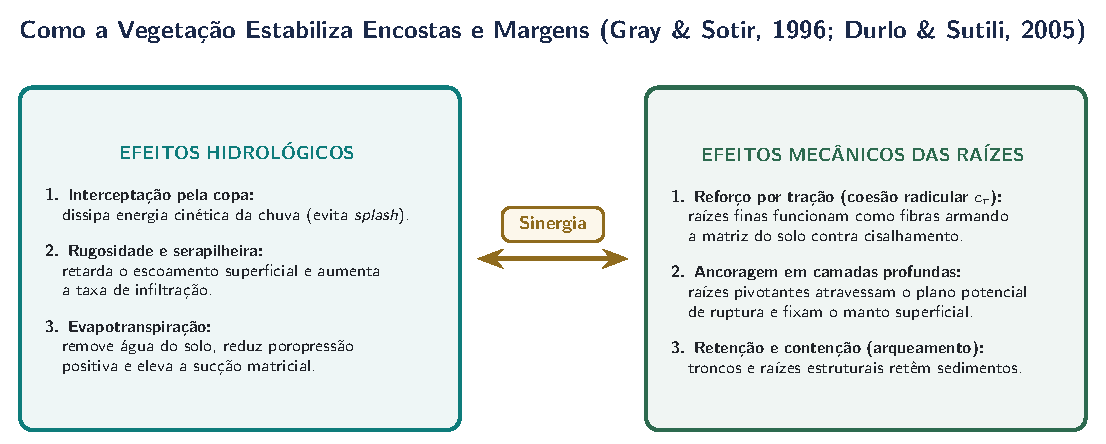
\includegraphics[width=0.92\textwidth]{figures/fig13_efeitos_raizes_solo.pdf}
  \caption{Integração dos efeitos mecânicos (tração radicular, ancoragem em camadas estáveis e arqueamento lateral) e efeitos hidrológicos (interceptação da copa, rugosidade superficial, infiltração e evapotranspiração) da vegetação na estabilização de encostas e margens.}
  \label{fig:efeitos_raizes_solo}
\end{figure}

No plano mecânico, conforme sistematizam Gray e Sotir (1996), as raízes estabilizam o solo por três mecanismos físicos complementares (Figura~\ref{fig:efeitos_raizes_solo}). Embora o solo possua elevada resistência à compressão, sua resistência à tração é reduzida; nesse contexto, as raízes finas e médias funcionam como fibras flexíveis de alta resistência à tração distribuídas na matriz terrosa, de modo que, quando uma zona potencial de cisalhamento tende a se deslocar, as raízes que atravessam esse plano são tensionadas e transferem parte do esforço para porções adjacentes estáveis, gerando o \textbf{reforço por tração radicular ($\Delta c_r$)}. Ao mesmo tempo, raízes pivotantes profundas atravessam horizontes superficiais mais friáveis e penetram em camadas subsuperficiais mais coesas ou fraturas do saprolito, promovendo \textbf{ancoragem em horizontes firmes} de modo análogo a microestacas naturais. Ademais, sistemas radiculares densos de árvores e arbustos distribuídos na vertente formam núcleos de maior rigidez que redistribuem as tensões laterais por \textbf{efeito de arqueamento}, restringindo o deslocamento de cunhas de solo entre os troncos.

No plano hidrológico, a cobertura vegetal protege o talude por uma sequência integrada de processos hidráulicos e edáficos. Inicialmente, as copas e a camada de serapilheira promovem a \textbf{interceptação} da chuva, amortecendo a energia cinética das gotas antes do contato com os agregados do solo e evitando a desagregação por salpicamento. Em seguida, os colmos, touceiras e detritos orgânicos aumentam a \textbf{rugosidade superficial} do terreno (elevando o coeficiente de rugosidade de Manning $n$), o que reduz a velocidade média do escoamento laminar e concentrado e diminui sua capacidade de arraste sólido. Ao longo do perfil, os bioporos abertos por raízes senescentes e pela fauna edáfica estimulam a \textbf{infiltração} e a recarga subsuperficial, ao passo que a \textbf{evapotranspiração} consome água da zona radicular entre eventos chuvosos, rebaixando o grau de saturação e a poropressão positiva ($u$) no interior do maciço.

\begin{boxFormula}[Critério de Mohr-Coulomb com Reforço Radicular ($\Delta c_r$)]
\begin{align}
  \tau &= (c' + c_r) + \sigma' \tan\phi' \qquad \text{com} \quad \sigma' = \sigma - u \\[4pt]
  FS &= \frac{\tau}{\tau_{\text{sol}}}
\end{align}
Nessa expressão, $\tau$ representa a resistência ao cisalhamento disponível no plano potencial de ruptura ($\text{kPa}$), $c'$ é a coesão efetiva intrínseca do solo ($\text{kPa}$, próxima de zero em solos arenosos puros), $c_r$ ($\Delta c_r$) traduz o reforço adicional conferido pelas raízes tracionadas ($\text{kPa}$), $\sigma'$ indica a tensão normal efetiva resultante da diferença entre a tensão total $\sigma$ e a pressão da água nos poros $u$ ($\text{kPa}$), e $\phi'$ expressa o ângulo de atrito interno efetivo (em graus). A razão $FS$ define o Fator de Segurança simplificado frente à tensão cisalhante solicitante $\tau_{\text{sol}}$.
\end{boxFormula}

Em projetos aplicados de controle erosivo, o reforço geotécnico das raízes na vertente e nos taludes articula-se diretamente ao disciplinamento hidráulico do talvegue (Figura~\ref{fig:mohr_coulomb_palicadas}). Enquanto a vegetação eleva a resistência ao cisalhamento $\tau_f$ ao acrescentar $c_r$ e reduzir a poropressão $u$ por sucção e evapotranspiração (Painel a), alcançando patamares de segurança superiores a $FS > 1{,}30$ sem impermeabilizar o terreno, as paliçadas permeáveis escalonadas pela regra pé-à-crista reduzem a declividade hidráulica efetiva do canal erodido e desaceleram o escoamento concentrado (Painel b).

\begin{figure}[H]
  \centering
  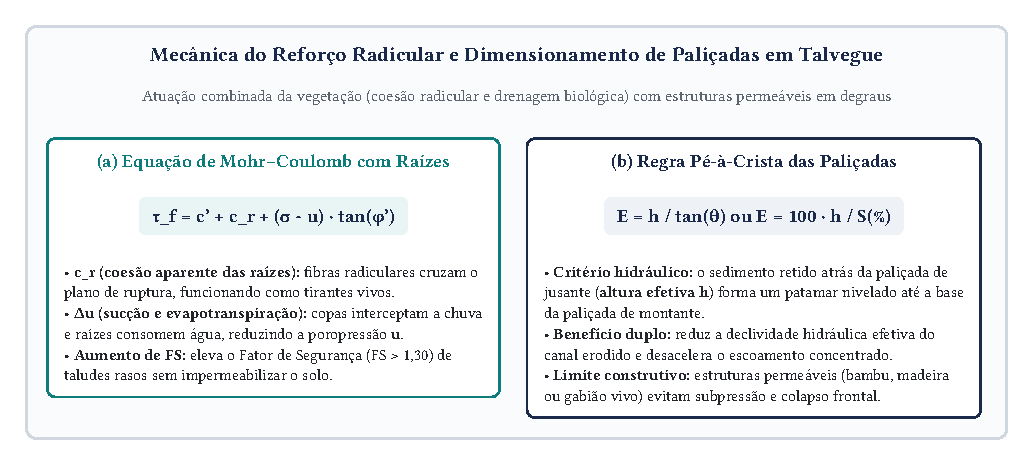
\includegraphics[width=0.94\textwidth]{figures/fig_cap13_mohr_coulomb_palicadas.pdf}
  \caption{Integração geotécnica e hidráulica na Bioengenharia de Solos, reunindo (a) os mecanismos da equação de Mohr-Coulomb vegetada e (b) a regra pé-à-crista de dimensionamento de paliçadas permeáveis em talvegue.}
  \label{fig:mohr_coulomb_palicadas}
\end{figure}

O Exemplo 13.1 quantifica exatamente como um incremento de coesão radicular $c_r$ altera o Fator de Segurança de um talude de corte exposto no Semiárido Baiano.

\begin{boxExemplo}{13.1 (Básico)}{Reforço Radicular na Equação de Mohr-Coulomb em Talude Degradado}
\passoEnunciado{Durante o diagnóstico de um talude de corte em solo argilo-arenoso ao longo de uma estrada de acesso no Semiárido Baiano, avalia-se o ganho de estabilidade proporcionado pela implantação de vegetação de enraizamento denso em comparação ao solo exposto.}
\passoDados{Coesão efetiva do solo $c' = 8{,}0\text{ kPa}$; ângulo de atrito efetivo $\phi' = 28^\circ$ ($\tan 28^\circ \approx 0{,}5317$); tensão normal efetiva no plano potencial de ruptura $\sigma' = 25{,}0\text{ kPa}$; reforço radicular medido para a espécie implantada $c_r = 6{,}5\text{ kPa}$; tensão cisalhante solicitante durante chuva intensa $\tau_{\text{sol}} = 23{,}0\text{ kPa}$.}
\passoPedido{Calcule a resistência ao cisalhamento sem vegetação ($\tau_0$) e com vegetação ($\tau_1$), o ganho percentual de resistência e o Fator de Segurança ($FS = \tau / \tau_{\text{sol}}$) nos dois cenários.}
\passoMetodo{Aplicação direta do critério de Mohr-Coulomb modificado pelo reforço radicular (Gray; Sotir, 1996), $\tau = (c' + c_r) + \sigma'\tan\phi'$.}
\passoContas{%
\textbf{Etapa 1, Parcela de atrito interno e resistência sem raízes ($c_r = 0$):}
\[
  \sigma' \tan\phi' = 25{,}0 \times 0{,}5317 = 13{,}29\text{ kPa} \qquad\qquad \tau_0 = 8{,}0 + 13{,}29 = 21{,}29\text{ kPa}
\]
\textbf{Etapa 2, Resistência com reforço radicular ($c_r = 6{,}5\text{ kPa}$) e ganho relativo:}
\[
  \tau_1 = (8{,}0 + 6{,}5) + 13{,}29 = 27{,}79\text{ kPa} \qquad\qquad \Delta_{\%} = \frac{27{,}79 - 21{,}29}{21{,}29} \times 100\% \approx 30{,}53\%
\]
\textbf{Etapa 3, Fator de Segurança ($FS$) nos dois cenários:}
\[
  FS_0 = \frac{21{,}29}{23{,}0} \approx 0{,}93 \quad (\text{instável, } FS < 1{,}0) \qquad\qquad FS_1 = \frac{27{,}79}{23{,}0} \approx 1{,}21 \quad (\text{estável, } FS > 1{,}0)
\]}
\passoResposta{Sem vegetação, $\tau_0 = 21{,}29\text{ kPa}$ ($FS_0 = 0{,}93$); com reforço radicular, $\tau_1 = 27{,}79\text{ kPa}$ ($FS_1 = 1{,}21$), representando ganho de $30{,}53\%$ na resistência ao cisalhamento.}
\passoVerificacao{O resultado é coerente com a física do solo, pois um incremento modesto de coesão radicular ($6{,}5\text{ kPa}$) converte um talude superficialmente instável ($FS < 1{,}0$) em estável ($FS > 1{,}2$) sob condição chuvosa crítica.}
\end{boxExemplo}

\section{Técnicas Vegetativas, Paliçadas Permeáveis e Biomantas Biodegradáveis}

A seleção das técnicas de bioengenharia depende da declividade da vertente, da presença de fluxo concentrado, da profundidade da incisão erosiva e das condições climáticas regionais. Em ambientes semiáridos, como a área de estudo da disciplina CHF662 na Bahia, o projeto deve considerar chuvas convectivas de alta intensidade seguidas por longos períodos de déficit hídrico, exigindo espécies e materiais capazes de resistir ao estresse hídrico inicial.

\subsection{Técnicas vegetativas lineares e de cobertura: estacas vivas, fascinas e trançados}

Entre as soluções que utilizam diretamente propágulos vegetativos lenhosos, as \textbf{estacas vivas (\textit{live stakes})} consistem em segmentos lenhosos ou semilenhosos de espécies com elevada capacidade de brotação, como gliricídia, sabiá, salgueiro em áreas úmidas ou espécies nativas propagáveis por estaquia, cravados perpendicularmente à superfície do talude ou levemente inclinados para jusante. Essas estacas funcionam como pinos biológicos que drenam o excesso de umidade superficial e ancoram mecanicamente os primeiros $0{,}4\text{ m}$ a $0{,}8\text{ m}$ de solo.

Quando há necessidade de barrar o transporte sólido ao longo da rampa, empregam-se \textbf{fascinas vivas (\textit{live fascines})}, formadas por feixes cilíndricos alongados de ramos vivos amarrados com arame ou corda de sisal e enterrados parcialmente em valas abertas em curva de nível na encosta ou na base de margens fluviais. Dispostas transversalmente ao escoamento, as fascinas atuam como pequenos terraços permeáveis contínuos que fragmentam o comprimento de rampa, retêm sedimentos finos e emitem raízes e brotos ao longo de todo o feixe. Em vertentes mais instáveis ou com maior mobilização superficial de solo, recorre-se aos \textbf{trançados vivos (\textit{wattle fences})}, que são cercas baixas construídas com estacas cravadas verticalmente e ramos flexíveis entrelaçados horizontalmente em curvas de nível, retendo o material erodido a montante e formando patamares de menor declividade favoráveis ao estabelecimento de mudas. O Exemplo 13.4 ilustra o dimensionamento integrado de estacas vivas e fascinas em um trecho de margem fluvial degradada.

\begin{boxExemplo}{13.4 (Intermediário)}{Dimensionamento de Estacas Vivas e Fascinas em Margem Fluvial}
\passoEnunciado{Um trecho de margem fluvial degradada apresenta solapamento na base e exposição do talude marginal. O projeto de recuperação combina fascinas vivas na zona de variação do nível d'água com plantio de estacas vivas na rampa superior.}
\passoDados{Extensão da margem $L = 180\text{ m}$; largura da faixa de rampa tratada com estacas vivas $w = 4{,}0\text{ m}$ (área $= 720\text{ m}^2$); espaçamento das estacas na rampa igual a $0{,}80\text{ m} \times 0{,}80\text{ m}$ ($0{,}64\text{ m}^2$ por estaca); $3$ linhas contínuas de fascinas na base ($3 \times 180 = 540\text{ m}$ lineares), fixadas por $1$ estaca a cada $0{,}75\text{ m}$; taxa média de pegamento esperada em campo igual a $75\%$.}
\passoPedido{Calcule o número de estacas na rampa, o número de estacas de fixação das fascinas, o total de estacas necessárias e a quantidade estimada de plantas vivas estabelecidas após o primeiro ciclo chuvoso.}
\passoMetodo{Razão entre área ou comprimento e espaçamento unitário, seguida da aplicação da taxa de sobrevivência.}
\passoContas{%
\textbf{Etapa 1, Estacas vivas na rampa ($720\text{ m}^2$) e ancoragem das fascinas ($540\text{ m}$):}
\[
  N_{\text{rampa}} = \frac{720}{0{,}64} = 1.125\text{ estacas} \qquad\qquad N_{\text{fasc}} = \frac{540}{0{,}75} = 720\text{ estacas}
\]
\textbf{Etapa 2, Total de estacas e estimativa de sobrevivência ($75\%$ de pegamento):}
\[
  N_{\text{total}} = 1.125 + 720 = 1.845\text{ estacas} \qquad\qquad N_{\text{vivas}} = 1.845 \times 0{,}75 = 1.383{,}75 \approx 1.384\text{ plantas vivas}
\]}
\passoResposta{São necessárias $1.125$ estacas na rampa e $720$ nas fascinas (total de $1.845$ estacas), resultando em aproximadamente $1.384$ plantas vivas estabelecidas.}
\passoVerificacao{Mesmo com $25\%$ de mortalidade inicial, permanecem cerca de $1{,}17\text{ planta}\cdot\text{m}^{-2}$ na rampa ($844/720$) e $3{,}0\text{ estacas}\cdot\text{m}^{-1}$ nas fascinas ao longo da margem ($540/180$), densidades adequadas para formar cobertura contínua na zona crítica.}
\end{boxExemplo}

Na escolha do material propagativo para essas técnicas vivas, a seleção botânica deve respeitar a ecologia da bacia hidrográfica e as exigências normativas de restauração.

\begin{boxErro}[Erro 1: Usar Espécies Exóticas Invasoras por Facilidade de Pegamento]
Fechar os taludes com espécies exóticas agressivas (como leucena ou gramíneas africanas invasoras) apenas pelo crescimento rápido compromete a sucessão ecológica nativa e viola diretrizes de PRAD em Áreas de Preservação Permanente. A escolha deve priorizar espécies nativas regionais ou coberturas anuais que cedam espaço às nativas.
\end{boxErro}

\subsection{Paliçadas e barragens permeáveis no controle de ravinas e voçorocas}

Quando a erosão já escavou sulcos profundos, ravinas ou voçorocas, coberturas superficiais isoladas perdem eficiência diante da energia cinética do fluxo concentrado. Nessa condição, implantam-se \textbf{paliçadas} (ou pequenas \textbf{barragens permeáveis} construídas com madeira, bambu, estacas vivas ou sacaria biodegradável preenchida com solo local), cuja disposição escalonada em série encontra-se representada na Figura~\ref{fig:bioengenharia_palicada_talude}. Ao permitir a passagem controlada da água pelos interstícios da estrutura enquanto retém as partículas sólidas transportadas por arraste e saltação, a paliçada reduz o empuxo hidrostático a montante e previne o colapso por pressão de água observado em barreiras impermeáveis.

\begin{figure}[H]
  \centering
  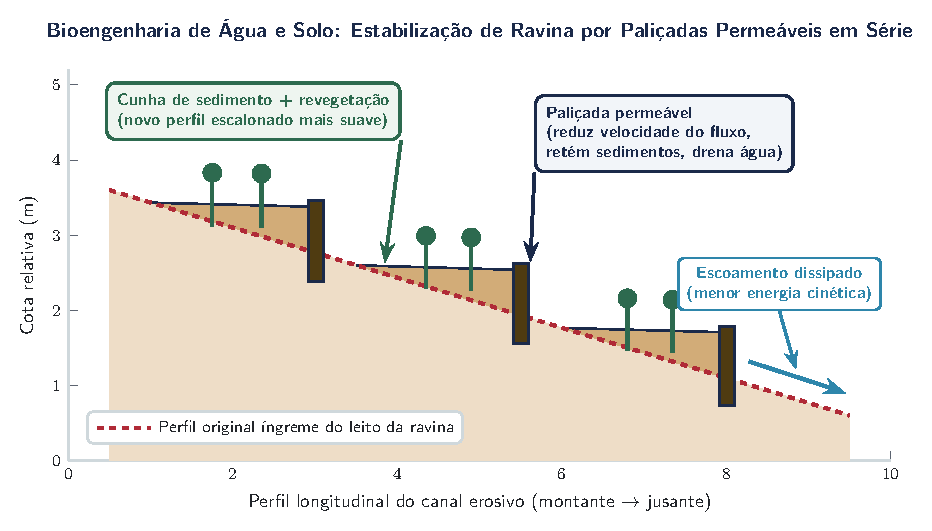
\includegraphics[width=0.94\textwidth]{figures/fig12_bioengenharia_palicada_talude.pdf}
  \caption{Esquema técnico de controle de erosão linear com paliçadas permeáveis escalonadas em série, evidenciando o espaçamento $E = h/S$, a cunha de sedimentos retidos a montante e o revestimento complementar de talude com biomanta e estacas vivas.}
  \label{fig:bioengenharia_palicada_talude}
\end{figure}

O acúmulo progressivo de sedimentos a montante de cada paliçada (Figura~\ref{fig:bioengenharia_palicada_talude}) reduz a declividade efetiva do leito da ravina, originando patamares estabilizados em forma de degraus vegetados que diminuem a velocidade da enxurrada e viabilizam a colonização vegetal no interior da antiga incisão, enquanto os taludes laterais recebem proteção complementar com biomanta e estacas vivas. Em solos muito friáveis ou trechos de curvas sinuosas, recomenda-se reduzir o espaçamento teórico em $15\%$ a $20\%$ como margem de segurança construtiva, verificando também a fundação e o engastamento lateral nas margens.

\begin{boxFormula}[Dimensionamento de Paliçadas: Espaçamento ($E$) e Cunha de Sedimentos ($V$)]
\begin{align}
  E &= \frac{h}{S} \qquad\qquad V = \frac{1}{2} \cdot L_m \cdot h \cdot b \qquad\qquad M = V \cdot \rho_s
\end{align}
Nessa formulação, $E$ expressa o espaçamento longitudinal entre paliçadas consecutivas ($\text{m}$) sob o critério pé-à-crista, $h$ é a altura útil da paliçada acima do leito ($\text{m}$) e $S$ indica a declividade longitudinal do canal em razão decimal ($\text{m}\cdot\text{m}^{-1}$, equivalente a $S(\%)/100$). Para o prisma triangular de sedimentos retidos a montante, $V$ representa o volume máximo retido por estrutura ($\text{m}^3$), $L_m$ indica o comprimento da cunha ($L_m = E$ no nivelamento teórico), $b$ é a largura média do canal ($\text{m}$), $\rho_s$ expressa a densidade aparente seca do sedimento ($\text{t}\cdot\text{m}^{-3}$) e $M$ fornece a massa de solo retida ($\text{t}$).
\end{boxFormula}

O Exemplo 13.2 demonstra o dimensionamento completo de uma série de paliçadas em uma ravina instalada a jusante de um bueiro rodoviário.

\begin{boxExemplo}{13.2 (Intermediário)}{Dimensionamento de Paliçadas Permeáveis e Volume de Sedimentos Retidos}
\passoEnunciado{Uma ravina ativa formada a jusante de um bueiro rodoviário apresenta risco de evoluir para voçoroca e assorear um riacho intermitente. A equipe técnica propõe instalar paliçadas de madeira e bambu em série ao longo do trecho mais íngreme.}
\passoDados{Comprimento total do trecho a tratar $L_t = 45{,}0\text{ m}$; declividade longitudinal média do leito da ravina $S = 8\%$ ($0{,}08\text{ m}\cdot\text{m}^{-1}$); altura útil adotada para cada paliçada $h = 0{,}60\text{ m}$; largura média da seção da ravina $b = 2{,}50\text{ m}$; densidade aparente do sedimento retido $\rho_s = 1{,}35\text{ t}\cdot\text{m}^{-3}$.}
\passoPedido{Determine o espaçamento teórico entre paliçadas ($E$), a quantidade de estruturas necessárias no trecho ($n$), o volume da cunha de sedimentos retido por paliçada ($V_1$), o volume total ($V_{\text{total}}$) e a massa total de sedimentos retida ($M$).}
\passoMetodo{Cálculo geométrico de perfil nivelado em degraus ($E = h/S$) e volume prismático triangular de cunha sedimentar ($V = \frac{1}{2}\cdot L_m \cdot h \cdot b$, com $L_m = E$).}
\passoContas{%
\textbf{Etapa 1, Espaçamento longitudinal ($E$) e número de paliçadas ($n$):}
\[
  E = \frac{h}{S} = \frac{0{,}60}{0{,}08} = 7{,}50\text{ m} \qquad\qquad n = \frac{L_t}{E} = \frac{45{,}0}{7{,}50} = 6\text{ paliçadas}
\]
\textbf{Etapa 2, Volume por paliçada ($L_m = E = 7{,}50\text{ m}$), volume total e massa retida:}
\[
  V_1 = \frac{1}{2} \cdot 7{,}50 \cdot 0{,}60 \cdot 2{,}50 = 5{,}625\text{ m}^3 \qquad V_{\text{total}} = 6 \times 5{,}625 = 33{,}75\text{ m}^3 \qquad M = 33{,}75 \times 1{,}35 = 45{,}56\text{ t}
\]}
\passoResposta{Espaçamento $E = 7{,}50\text{ m}$; $n = 6$ paliçadas; $V_1 = 5{,}625\text{ m}^3$ por estrutura; volume total retido $V_{\text{total}} = 33{,}75\text{ m}^3$, equivalente a $45{,}56\text{ t}$ de sedimentos.}
\passoVerificacao{Seis estruturas de $0{,}60\text{ m}$ de altura acumulam um desnível total de $6 \times 0{,}60 = 3{,}60\text{ m}$, igual ao desnível natural do trecho de $45{,}0\text{ m}$ a $8\%$ ($45{,}0 \times 0{,}08 = 3{,}60\text{ m}$), fechando geometricamente o escalonamento.}
\end{boxExemplo}

Na implantação em campo, um dos erros executivos mais destrutivos consiste em vedar completamente a seção da paliçada, convertendo-a em uma barreira estanque sujeita a transbordamento lateral.

\begin{boxErro}[Erro 2: Construir Paliçadas Impermeáveis Sem Dissipação de Energia]
Fechar totalmente a seção da ravina com chapas rígidas, alvenaria sem drenos ou lonas plásticas cria empuxo hidrostático excessivo a montante e transbordamento concentrado pelas laterais, provocando erosão regressiva nas ombreiras e destruição da obra logo na primeira enxurrada intensa. Paliçadas devem ser \textbf{permeáveis} e devidamente engastadas nas paredes laterais da ravina.
\end{boxErro}

\subsection{Biomantas, geotêxteis biodegradáveis e evidências experimentais de campo}

Em taludes recém-conformados, platôs de obras lineares ou áreas submetidas a hidrossemeadura, as \textbf{biomantas} e os \textbf{geotêxteis biodegradáveis} oferecem proteção imediata ao solo exposto por meio de mantas tecidas ou costuradas com fibras vegetais naturais. Na realidade produtiva do Nordeste brasileiro, a \textbf{fibra de sisal (\textit{Agave sisalana})}, amplamente disponível na Bahia, destaca-se pela boa resistência mecânica inicial e decomposição moderada entre $12$ e $24$ meses, integrando a bioengenharia à economia regional do Semiárido. Em taludes mais íngremes e margens submetidas a fluxos intermitentes mais energéticos, recomenda-se a \textbf{fibra de coco (\textit{Cocos nucifera})}, cuja elevada proporção de lignina assegura longevidade funcional entre $24$ e $48$ meses. Já as mantas de \textbf{fibra de taboa (\textit{Typha domingensis}) e juta} constituem materiais leves e altamente higroscópicos, indicados para reter umidade na camada superficial em climas secos e proteger encostas de baixa a média declividade até a germinação do estrato herbáceo. Associam-se às biomantas os \textbf{retentores de sedimentos} (biorretentores cilíndricos preenchidos com palha, fibra de coco ou casca de arroz, dispostos em curvas de nível ou na base de taludes) e a \textbf{revegetação estratificada}, combinando gramíneas de cobertura rápida, leguminosas fixadoras de nitrogênio e espécies arbustivo-arbóreas nativas.

A eficácia desses geomateriais depende diretamente da arquitetura das fibras e da continuidade do contato com o substrato mineral (Figura~\ref{fig:geocomposito_estrutura}). Em um geocompósito trilayer de fibras naturais estudado experimentalmente por Santos e colaboradores, a trama estruturada estabiliza o núcleo fibroso e mantém contato íntimo com os agregados do solo, evitando o escoamento concentrado sob a manta e os descolamentos durante a degradação em campo.

\begin{figure}[H]
  \centering
  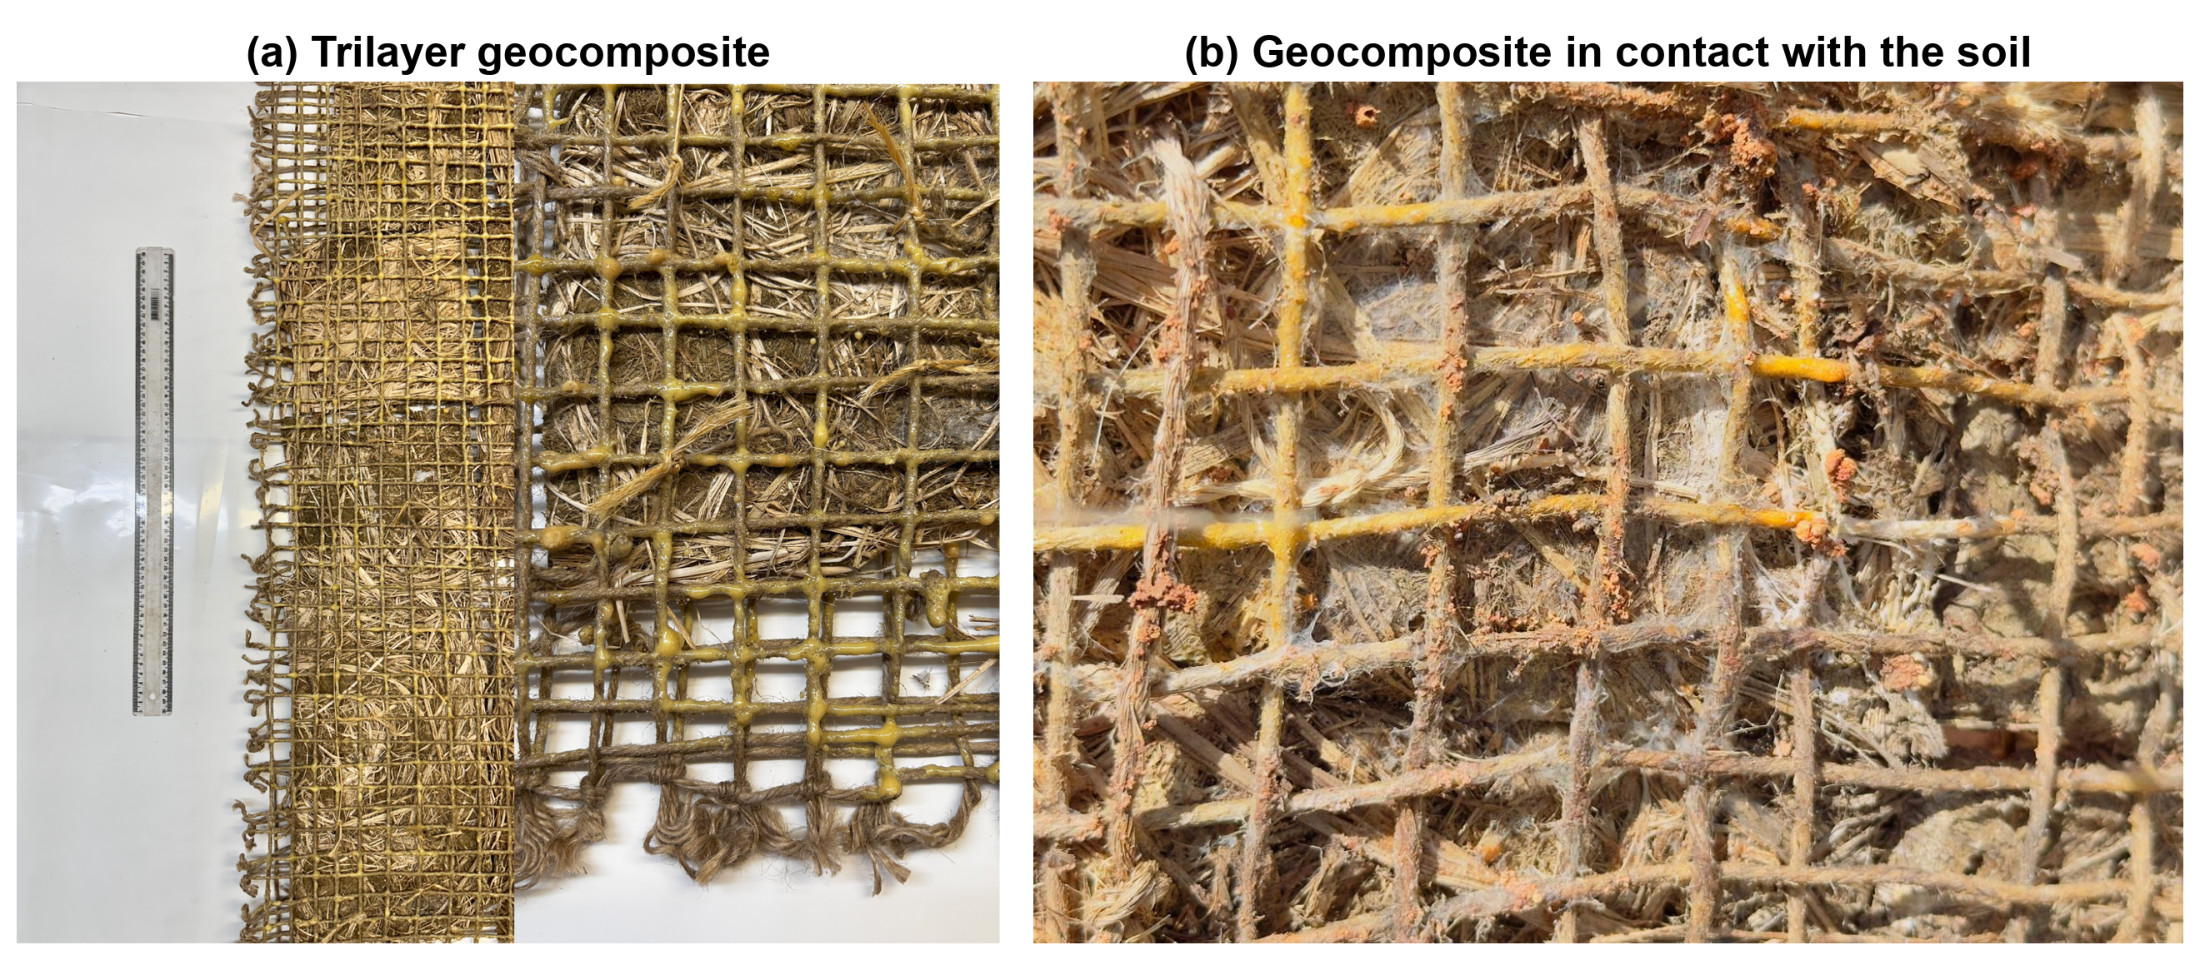
\includegraphics[width=0.90\textwidth]{figures/artigo_geocomposito_estrutura.jpg}
  \caption{Arquitetura de geocompósito trilayer de fibras naturais (a) e interface de contato direto com a superfície do solo (b). Fonte: Reprodução didática de estudo experimental em campo com vetiver e geocompósito trilayer (acervo fornecido pelos autores).}
  \label{fig:geocomposito_estrutura}
\end{figure}

Quando associados ao estabelecimento de gramíneas cespitosas de enraizamento profundo, como o capim-vetiver em parcelas experimentais delimitadas com coletores de enxurrada e sedimentos na base do talude (Figura~\ref{fig:geocomposito_campo}), esses sistemas permitem quantificar conjuntamente a integridade do geomaterial, a taxa de sobrevivência vegetal e a redução de carga sólida frente a eventos reais de precipitação.

\begin{figure}[H]
  \centering
  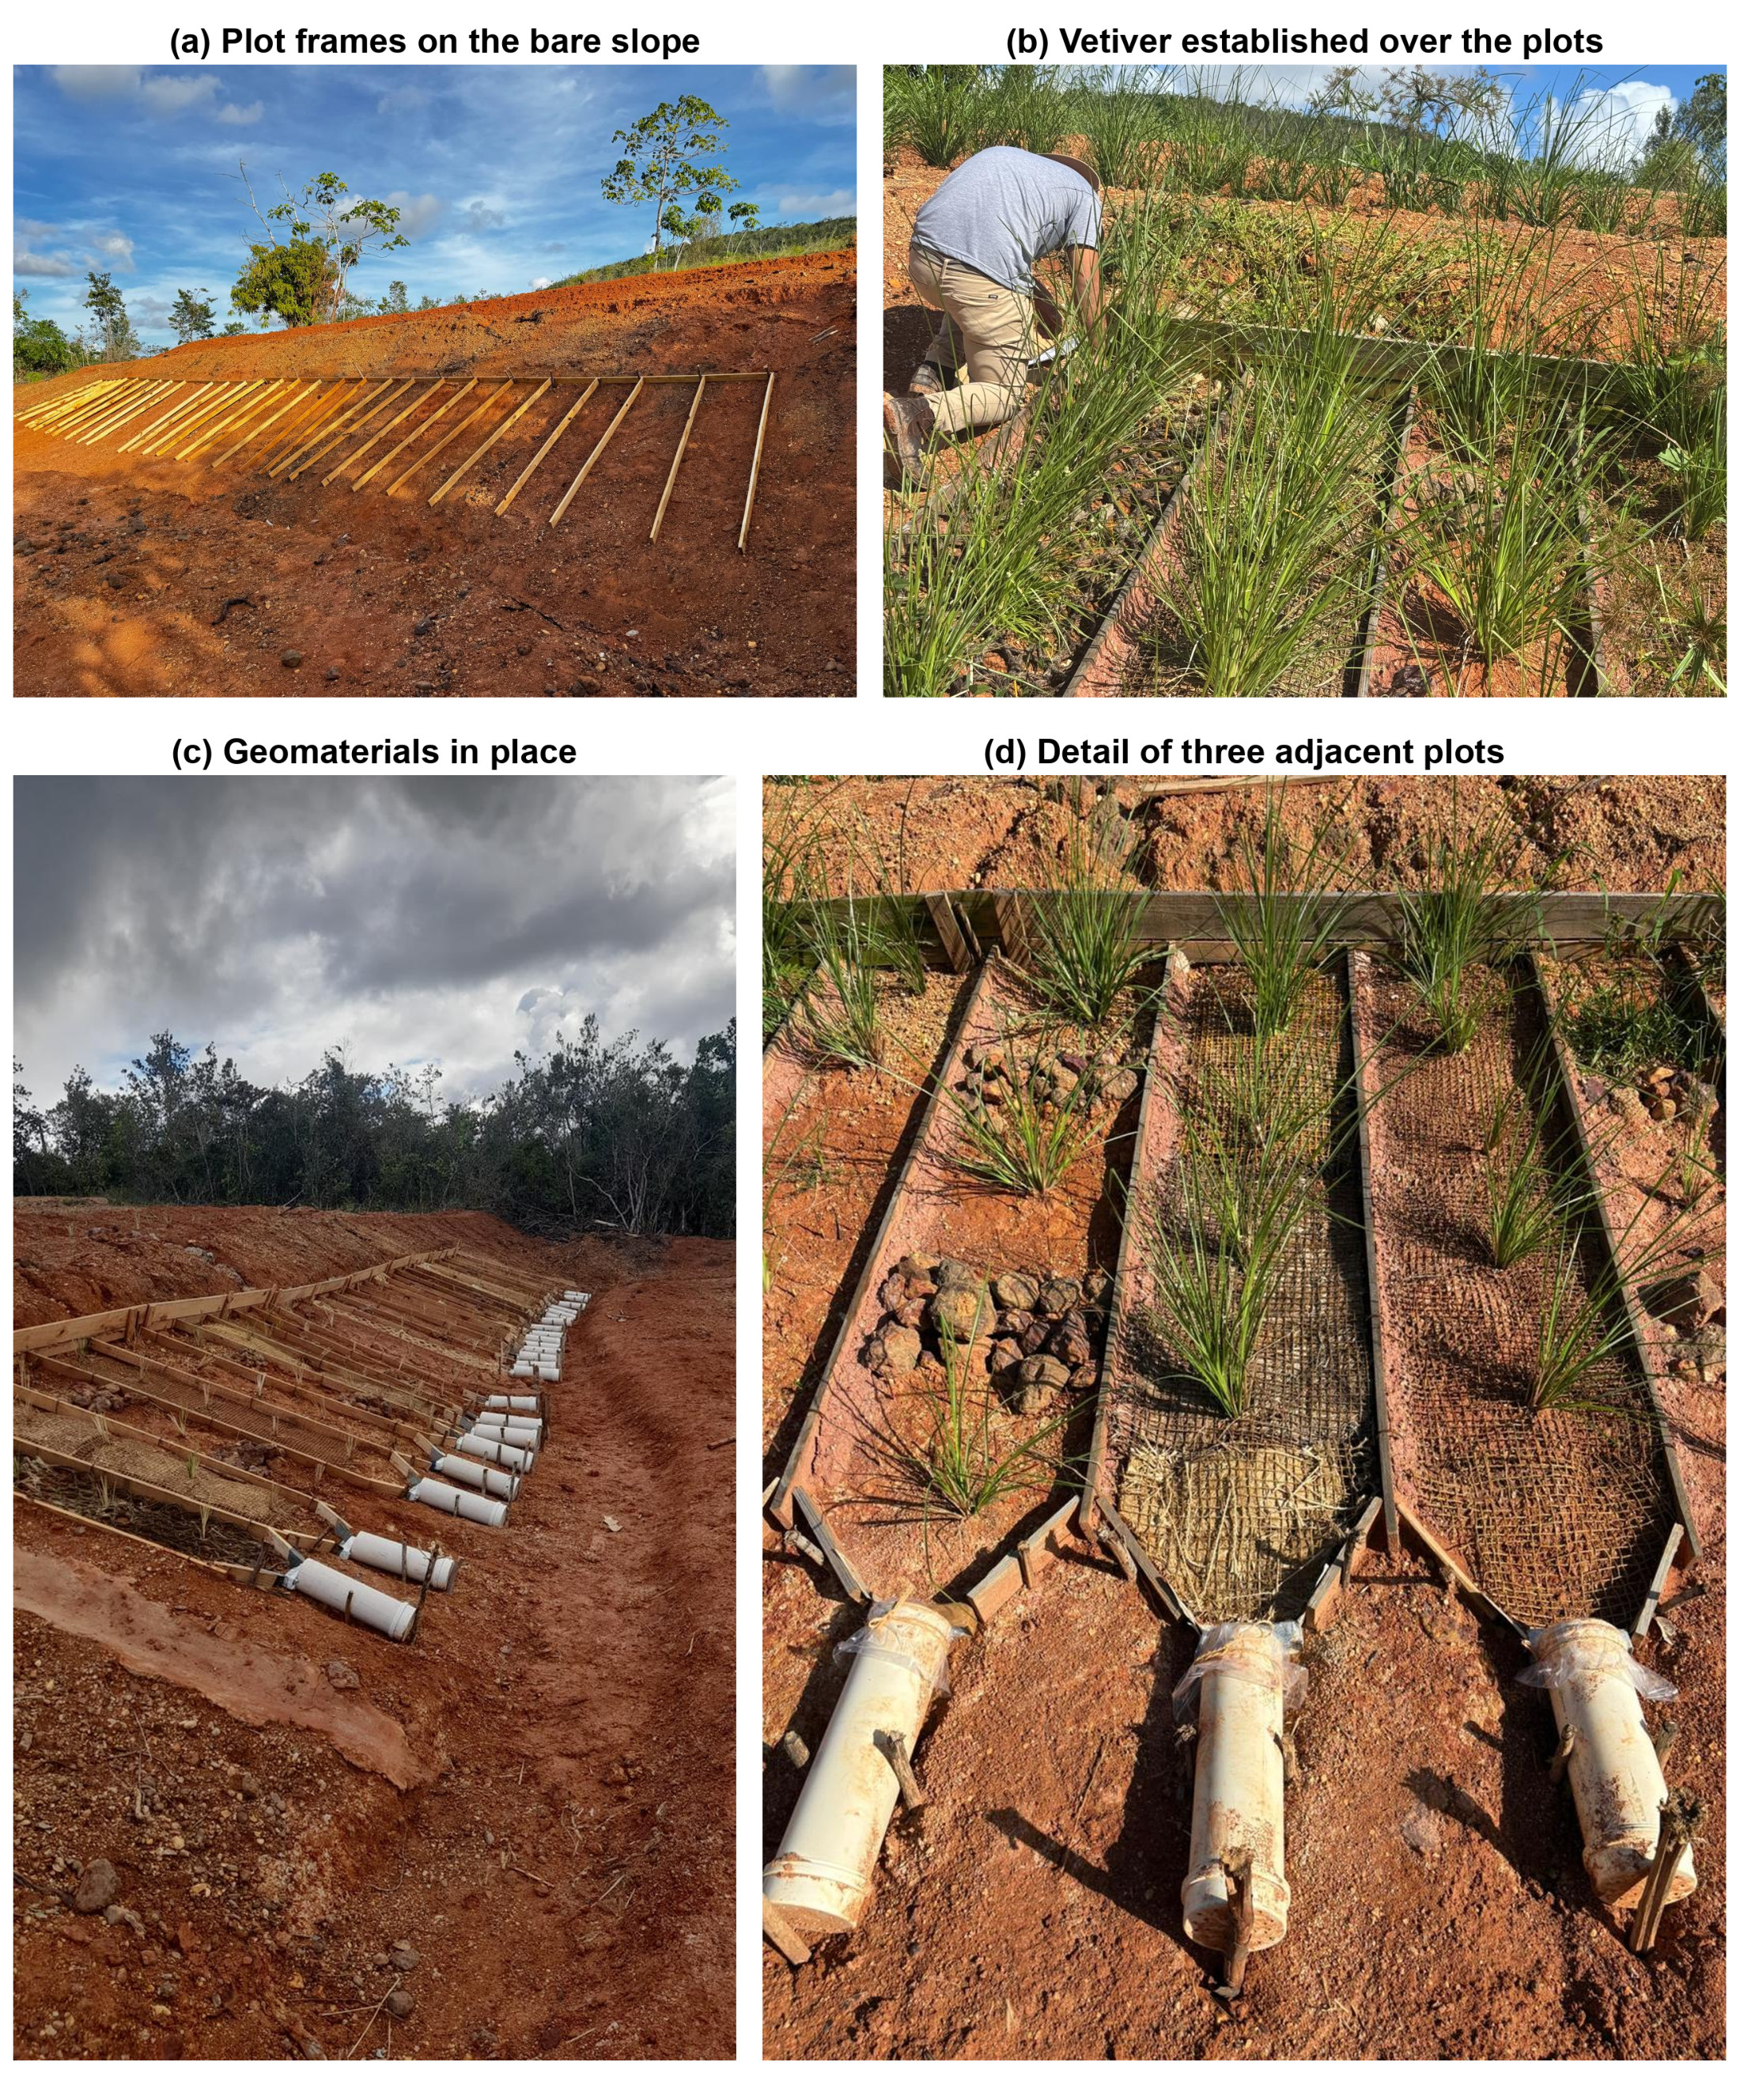
\includegraphics[width=0.88\textwidth]{figures/artigo_geocomposito_campo.jpg}
  \caption{Implantação de parcelas experimentais em talude degradado com capim-vetiver, geomateriais biodegradáveis e coletores hidrossedimentológicos. Fonte: Reprodução didática de estudo experimental em campo com vetiver e geocompósito trilayer (acervo fornecido pelos autores; painéis originais preservados).}
  \label{fig:geocomposito_campo}
\end{figure}

O Exemplo 13.3 mostra como dimensionar a aquisição de rolos de biomanta de sisal e estimar a massa anual de solo retida em um talude de corte no Semiárido.

\begin{boxExemplo}{13.3 (Intermediário)}{Proteção Superficial com Biomanta de Sisal e Redução de Perda de Solo}
\passoEnunciado{Um talude de corte recém-terraplenado em um empreendimento eólico no Semiárido apresenta perda de solo acentuada nos primeiros meses chuvosos. Para conter a erosão laminar e viabilizar o estabelecimento de gramíneas e leguminosas, prescreve-se a aplicação de biomanta de fibra de sisal associada à hidrossemeadura.}
\passoDados{Área do talude $A = 1.200\text{ m}^2$ ($0{,}12\text{ ha}$); taxa de perda de solo sem proteção medida por pinos de erosão igual a $45{,}0\text{ t}\cdot\text{ha}^{-1}\cdot\text{ano}^{-1}$; eficiência de redução da perda de solo pela biomanta de sisal igual a $85\%$; dimensões comerciais do rolo de biomanta iguais a $2{,}0\text{ m} \times 25{,}0\text{ m}$ ($50{,}0\text{ m}^2$ por rolo), exigindo $10\%$ de acréscimo de área para sobreposição das emendas.}
\passoPedido{Calcule a perda anual de solo sem proteção e com biomanta (em $\text{t}\cdot\text{ano}^{-1}$), a massa de solo retida anualmente na encosta e o número mínimo inteiro de rolos de biomanta a adquirir.}
\passoMetodo{Conversão de área para hectares, aplicação do fator de atenuação erosiva ($1 - 0{,}85 = 0{,}15$) e dimensionamento de cobertura com sobreposição.}
\passoContas{%
\textbf{Etapa 1, Perda sem proteção ($P_0$), perda residual ($P_1$) e massa retida ($\Delta P$):}
\begin{align*}
  P_0 &= 0{,}12 \times 45{,}0 = 5{,}40\text{ t}\cdot\text{ano}^{-1} \qquad P_1 = 5{,}40 \times 0{,}15 = 0{,}81\text{ t}\cdot\text{ano}^{-1} \\
  \Delta P &= 5{,}40 - 0{,}81 = 4{,}59\text{ t}\cdot\text{ano}^{-1}
\end{align*}
\textbf{Etapa 2, Área efetiva com $10\%$ de sobreposição e quantidade de rolos:}
\begin{align*}
  A_{\text{ef}} &= 1.200 \times 1{,}10 = 1.320\text{ m}^2 \\
  N_{\text{rolos}} &= \frac{1.320}{50{,}0} = 26{,}4 \rightarrow \mathbf{27\text{ rolos}}
\end{align*}}
\passoResposta{A perda cai de $5{,}40\text{ t}\cdot\text{ano}^{-1}$ para $0{,}81\text{ t}\cdot\text{ano}^{-1}$ (retenção de $4{,}59\text{ t}\cdot\text{ano}^{-1}$); devem ser adquiridos $27$ rolos de biomanta de sisal.}
\passoVerificacao{O arredondamento para cima ($27$ rolos) garante que não falte material nas bordas de ancoragem em valas de coroamento e pé de talude, prática obrigatória em especificações executivas.}
\end{boxExemplo}

Na instalação dessas coberturas em taludes, o desempenho medido em experimentos só se repete em obras reais quando o substrato é previamente regularizado e grampeado de forma contínua.

\begin{boxErro}[Erro 3: Aplicar Biomanta Sem Contato Íntimo com o Solo Preparado]
Estender biomantas sobre superfície irregular cheia de torrões, pedras soltas ou sulcos não regularizados deixa bolsões de ar sob a manta. A água da chuva escoa por baixo da biomanta, escava o solo invisivelmente e impede que as raízes das sementes germinadas alcancem o substrato mineral. O preparo, a regularização e o grampeamento firme ao solo são obrigatórios.
\end{boxErro}

\section{Comparação Técnica e Econômica com Obras Cinzas Rígidas}

A escolha entre soluções baseadas na natureza e obras convencionais de engenharia civil pauta-se por critérios técnicos, geotécnicos e econômicos objetivos. Em encostas com risco geotécnico imediato sobre edificações críticas ou em gargantas fluviais submetidas a velocidades hidráulicas extremas, estruturas rígidas de concreto ou alvenaria mostram-se indispensáveis. Entretanto, na maior parte das áreas degradadas rurais, faixas de domínio e margens fluviais, a bioengenharia apresenta vantagens estruturais e ecológicas consistentes ao longo do ciclo de vida do projeto.

No que toca à \textbf{evolução do desempenho e à interação hidrológica}, soluções de bioengenharia exibem resistência crescente com o tempo, pois o desenvolvimento radicular amplia $\Delta c_r$ e a cobertura aérea amortece o salpicamento, enquanto estruturas rígidas sofrem fadiga, fissuração e solapamento progressivo sem capacidade de autorreparação. Além disso, sistemas vegetados mantêm a permeabilidade do substrato, favorecem a infiltração, aliviam poropressões ($u$) e atenuam picos de cheia a jusante, ao passo que revestimentos impermeáveis exigem redes complexas de drenos e tendem a transferir energia cinética erosiva para trechos inferiores.

Sob a perspectiva de \textbf{custo, manutenção e conformidade legal}, obras de bioengenharia reduzem em $30\%$ a $75\%$ o investimento inicial em taludes e ravinas por mobilizarem mão de obra e insumos vegetais locais, dispensando escavações profundas, aço e concreto. Embora demandem maior atenção nos primeiros $12$ a $24$ meses para irrigação de pegamento, replantio e controle de formigas cortadeiras, sua longevidade restaura funções ecossistêmicas, conectividade ripária e metas legais de PRAD em APPs. O acompanhamento pós-obra deve registrar sobrevivência, cobertura vegetal, integridade dos materiais e alteração das seções em referências fixas após eventos de chuva, distinguindo deposição temporária de estabilização definitiva.

\etapa{4}{Síntese Aplicada: Análise Comparativa de Custo e Desempenho}

Para fechar a avaliação de viabilidade de um projeto de recuperação, o analista ambiental confronta o orçamento de implantação e manutenção das alternativas frente aos benefícios hidrológicos e ecológicos esperados na área de intervenção, como exemplificado a seguir.

\begin{boxExemplo}{13.5 (Avançado)}{Análise Comparativa de Custo e Desempenho: Bioengenharia vs. Obra Cinza}
\passoEnunciado{A prefeitura de um município baiano precisa estabilizar $100\text{ m}$ de talude marginal de uma estrada vicinal que dá acesso a uma área de captação de água, evitando o assoreamento do manancial.}
\passoDados{Extensão do trecho $L = 100\text{ m}$; altura do talude $h = 3{,}0\text{ m}$. Alternativa A (obra cinza rígida em muro de concreto ou gabião argamassado) com custo unitário de $\reais{1.850{,}00}\cdot\text{m}^{-1}$. Alternativa B (bioengenharia com retentores de sedimentos na base, biomanta de coco e estacas vivas nativas) com custo de implantação de $\reais{420{,}00}\cdot\text{m}^{-1}$ mais plano de manutenção de $2$ anos orçado em $\reais{8.000{,}00}$ no total.}
\passoPedido{Calcule o custo total de cada alternativa, a economia financeira absoluta e percentual proporcionada pela bioengenharia e justifique a escolha sob a ótica hidrogeomorfológica.}
\passoMetodo{Orçamentação linear direta e comparação relativa de custos associada à análise de serviços ecossistêmicos.}
\passoContas{%
\textbf{Etapa 1, Custo total da Alternativa A ($C_A$) e da Alternativa B ($C_B$):}
\[
  C_A = 100 \times 1.850{,}00 = \reais{185.000{,}00} \qquad\qquad C_B = (100 \times 420{,}00) + 8.000{,}00 = \reais{50.000{,}00}
\]
\textbf{Etapa 2, Economia financeira absoluta ($\Delta C$) e percentual ($\Delta C_{\%}$):}
\[
  \Delta C = 185.000{,}00 - 50.000{,}00 = \reais{135.000{,}00} \qquad\qquad \Delta C_{\%} = \frac{135.000{,}00}{185.000{,}00} \times 100\% \approx 72{,}97\%
\]}
\passoResposta{Alternativa A de $\reais{185.000{,}00}$ e Alternativa B de $\reais{50.000{,}00}$. A bioengenharia gera economia de $\reais{135.000{,}00}$ ($72{,}97\%$), além de preservar a infiltração na zona de recarga do manancial.}
\passoVerificacao{A economia de $72{,}97\%$ é compatível com a literatura de Engenharia Natural para taludes de média altura ($3{,}0\text{ m}$) sem cargas estruturais de edificações no coroamento.}
\end{boxExemplo}

\etapa{5}{Armadilha Conceitual e Materiais Audiovisuais de Apoio}

Mesmo quando o dimensionamento geotécnico e hidráulico está correto, a descontinuidade nos tratos culturais iniciais pode comprometer todo o estabelecimento vegetal em regiões sujeitas a veranicos prolongados.

\begin{boxErro}[Erro 4: Ignorar o Esforço de Manutenção Pós-Plantio no Semiárido]
Em regiões de baixa pluviosidade irregular, abandonar estacas, mudas ou biomantas sem controle de formigas cortadeiras, proteção contra pisoteio de rebanhos e irrigação de salvamento nos primeiros meses leva a taxas de mortalidade superiores a $80\%$, anulando o investimento inicial antes que o reforço radicular $c_r$ se estabeleça.
\end{boxErro}

Para aprofundar o estudo das práticas vegetativas, estruturas permeáveis e Soluções Baseadas na Natureza, assista às videoaulas selecionadas na página da disciplina, iniciando por \textit{Erosão Hídrica e Processos da Erosão} (\url{https://www.youtube.com/watch?v=6cjHYL6yuzE}), \textit{Práticas para o controle da erosão hídrica - Parte 1} (\url{https://www.youtube.com/watch?v=vsKm_cG8KkI}) e \textit{Uso do Solo, Erosão e Técnicas de Conservação} (\url{https://www.youtube.com/watch?v=0w_ZhulcorU}), e complementando com \textit{Soluções Baseadas na Natureza (SbN)} (\url{https://www.youtube.com/watch?v=Cvd2roRDY40}) e \textit{Medidas Estruturais de Baixo Impacto: Soluções Baseadas na Natureza} (\url{https://www.youtube.com/watch?v=vQtOYoXyNOI}).

\etapa{6}{Exercícios de Fixação (15 Questões)}

\subsection*{Bloco A: Questões Conceituais Básicas (1 a 5)}
\begin{enumerate}[leftmargin=1.8em, itemsep=6pt]
  \item Explique o princípio da substituição gradual de funções entre materiais inertes biodegradáveis e elementos vivos na Bioengenharia de Solos.
  \espacoResolucao[1.8cm]

  \item Diferencie o papel mecânico do reforço por tração radicular ($c_r$) do mecanismo de ancoragem profunda das raízes em uma encosta inclinada.
  \espacoResolucao[1.8cm]

  \item Descreva três efeitos hidrológicos da vegetação que contribuem para aumentar a estabilidade de um talude e reduzir o escoamento superficial.
  \espacoResolucao[1.8cm]

  \item Compare as finalidades construtivas de estacas vivas, fascinas e trançados vivos na recuperação de vertentes degradadas.
  \espacoResolucao[1.8cm]

  \item Cite três vantagens ambientais e econômicas das biomantas de fibra de sisal ou coco em comparação com o revestimento rígido em concreto projetado.
  \espacoResolucao[1.8cm]
\end{enumerate}

\subsection*{Bloco B: Questões Intermediárias e Quantitativas (6 a 10)}
\begin{enumerate}[leftmargin=1.8em, itemsep=6pt, start=6]
  \item Um solo apresenta coesão efetiva $c' = 6{,}0\text{ kPa}$, tensão normal efetiva $\sigma' = 20{,}0\text{ kPa}$ e $\tan\phi' = 0{,}50$. Calcule a resistência ao cisalhamento sem vegetação ($\tau_0$) e com reforço radicular $c_r = 5{,}0\text{ kPa}$ ($\tau_1$), indicando o ganho percentual obtido.
  \espacoResolucao[2.1cm]

  \item Uma ravina com declividade longitudinal $S = 0{,}10\text{ m}\cdot\text{m}^{-1}$ ($10\%$) será estabilizada com paliçadas de madeira de altura útil $h = 0{,}50\text{ m}$ e largura média $b = 2{,}00\text{ m}$. Calcule o espaçamento teórico $E$ entre as paliçadas e o volume de sedimentos retido na cunha de uma paliçada ($L_m = E$).
  \espacoResolucao[2.1cm]

  \item Em um trecho de $36{,}0\text{ m}$ de uma voçoroca com declividade $S = 0{,}05\text{ m}\cdot\text{m}^{-1}$, deseja-se instalar paliçadas com altura útil $h = 0{,}45\text{ m}$ e largura média $b = 1{,}80\text{ m}$. Determine o espaçamento $E$, o número de paliçadas necessárias e a massa total de sedimentos retida considerando $\rho_s = 1{,}40\text{ t}\cdot\text{m}^{-3}$.
  \espacoResolucao[2.1cm]

  \item Um talude de $2.500\text{ m}^2$ será protegido com biomanta de fibra de coco vendida em rolos de $2{,}0\text{ m} \times 30{,}0\text{ m}$ ($60\text{ m}^2$ por rolo), prevendo-se $8\%$ de perda por sobreposição de emendas e ancoragem em valas. Calcule a quantidade mínima inteira de rolos necessários.
  \espacoResolucao[2.1cm]

  \item Uma faixa de margem fluvial de $120\text{ m}$ de extensão e $5{,}0\text{ m}$ de largura ($600\text{ m}^2$) receberá estacas vivas no espaçamento de $1{,}0\text{ m} \times 0{,}60\text{ m}$ ($0{,}60\text{ m}^2$ por estaca). Sabendo que a sobrevivência esperada é de $80\%$, quantas estacas devem ser plantadas e quantas plantas vivas deverão permanecer estabelecidas?
  \espacoResolucao[2.1cm]
\end{enumerate}

\subsection*{Bloco C: Questões Objetivas de Múltipla Escolha (11 a 15)}
\begin{enumerate}[leftmargin=1.8em, itemsep=6pt, start=11]
  \item Na equação de Mohr-Coulomb modificada para solos vegetados, $\tau = (c' + c_r) + \sigma'\tan\phi'$, o termo $c_r$ representa:
  \begin{alternativas}
    \item A pressão neutra da água acumulada nos poros do solo durante a chuva.
    \item A redução do ângulo de atrito interno causada pelo crescimento radicular.
    \item A coesão aparente adicional conferida pela resistência à tração das raízes que cruzam o plano de ruptura.
    \item O peso próprio da copa das árvores atuando como sobrecarga vertical.
    \item A impermeabilização superficial gerada pela serapilheira em decomposição.
  \end{alternativas}
  \espacoResolucao[1.2cm]

  \item Uma ravina com declividade $S = 12\%$ ($0{,}12$) será tratada com paliçadas permeáveis de altura útil $h = 0{,}60\text{ m}$. O espaçamento teórico $E$ entre duas paliçadas consecutivas é:
  \begin{alternativas}
    \item $2{,}00\text{ m}$.
    \item $3{,}60\text{ m}$.
    \item $5{,}00\text{ m}$.
    \item $7{,}20\text{ m}$.
    \item $12{,}00\text{ m}$.
  \end{alternativas}
  \espacoResolucao[1.2cm]

  \item Considerando uma paliçada com altura útil $h = 0{,}50\text{ m}$, largura do canal $b = 2{,}40\text{ m}$ e comprimento da cunha retida a montante $L_m = 6{,}00\text{ m}$, o volume máximo de sedimentos retido por essa estrutura é:
  \begin{alternativas}
    \item $1{,}80\text{ m}^3$.
    \item $3{,}60\text{ m}^3$.
    \item $5{,}40\text{ m}^3$.
    \item $7{,}20\text{ m}^3$.
    \item $14{,}40\text{ m}^3$.
  \end{alternativas}
  \espacoResolucao[1.2cm]

  \item Sobre as fibras vegetais empregadas em biomantas e geotêxteis biodegradáveis no Brasil, assinale a alternativa correta:
  \begin{alternativas}
    \item A fibra de coco possui menor teor de lignina que a palha de arroz e degrada-se em menos de 30 dias.
    \item O sisal (\textit{Agave sisalana}) é uma fibra regionalmente estratégica no Semiárido Baiano e protege o solo contra o impacto das gotas até o estabelecimento da vegetação.
    \item As biomantas dispensam qualquer contato com o solo, devendo permanecer suspensas a $20\text{ cm}$ da superfície.
    \item Geotêxteis biodegradáveis impedem totalmente a infiltração da água pluvial, comportando-se como lonas de polietileno.
    \item A aplicação de biomantas é tecnicamente incompatível com hidrossemeadura ou plantio de mudas.
  \end{alternativas}
  \espacoResolucao[1.2cm]

  \item Em comparação com muros rígidos de concreto armado utilizados na contenção de margens fluviais rurais, uma solução de bioengenharia com fascinas vivas e estacas vivas caracteriza-se por:
  \begin{alternativas}
    \item Apresentar resistência estrutural decrescente desde o primeiro mês após a implantação.
    \item Impedir a troca de água entre o canal fluvial e o lençol freático marginal.
    \item Exigir maior consumo de cimento e aço por metro linear de margem protegida.
    \item Aumentar progressivamente a estabilidade com o enraizamento, manter a permeabilidade da margem e restaurar o habitat ripário.
    \item Eliminar a necessidade de qualquer cuidado com espécies invasoras ou formigas cortadeiras nos primeiros meses.
  \end{alternativas}
  \espacoResolucao[1.2cm]
\end{enumerate}

\etapa{7}{Questões no Estilo ENADE e Concursos Ambientais}

\begin{boxDica}[Foco de Provas, ENADE e Concursos Ambientais]
Bancas como CESPE/Cebraspe, FGV e o exame do ENADE valorizam a integração entre processo físico (erosão, cisalhamento, poropressão) e escolha da técnica de recuperação. Ao analisar estudos de caso, verifique se a técnica proposta atua sobre a causa hidrológica e mecânica do processo.
\end{boxDica}

\begin{enumerate}[leftmargin=1.8em, itemsep=7pt]
  \item \textbf{[Questão Autoral, Estilo ENADE / Geografia]} Após a implantação de um parque eólico em área de chapada semiárida, verificou-se a abertura de ravinas em taludes de corte de estradas de acesso, com carreamento de sedimentos para um riacho intermitente. Como solução, um técnico propôs substituir um projeto de canaletas e muros de concreto por um arranjo de bioengenharia combinando biomantas de sisal nos taludes, retentores de sedimentos no pé das rampas e paliçadas permeáveis escalonadas nas incisões. Considerando os princípios da Engenharia Natural, avalie as asserções:
  \begin{itemize}[leftmargin=1.4em, itemsep=2pt]
    \item[I.] A biomanta de sisal reduz imediatamente a energia cinética do salpicamento (\textit{splash}) e mantém a umidade superficial necessária à germinação de sementes nativas.
    \item[II.] As paliçadas permeáveis dissipam a energia do fluxo concentrado sem gerar empuxo hidrostático excessivo e formam patamares de sedimentos favoráveis à revegetação interna da ravina.
    \item[III.] A substituição de obras cinzas por bioengenharia elimina completamente a necessidade de drenagem de águas pluviais oriundas da pista compactada da estrada.
  \end{itemize}
  É correto o que se afirma em:
  \begin{alternativas}
    \item I, apenas.
    \item III, apenas.
    \item I e II, apenas.
    \item II e III, apenas.
    \item I, II e III.
  \end{alternativas}

  \item \textbf{[Questão Autoral, Estilo Concurso Analista Ambiental / INEMA-BA]} Em um projeto de recuperação de área degradada (PRAD) em margem fluvial de bacia hidrográfica baiana, deseja-se aumentar a estabilidade do talude marginal contra escorregamentos rasos durante cheias sazonais. À luz da equação $\tau = (c' + c_r) + (\sigma - u)\tan\phi'$, qual combinação de mecanismos explica corretamente o efeito benéfico da vegetação ripária estabelecida?
  \begin{alternativas}
    \item As raízes anulam a coesão efetiva $c'$ e elevam a poropressão $u$, reduzindo o atrito interno $\phi'$.
    \item O reforço radicular acrescenta coesão aparente $c_r$ por resistência à tração das fibras no plano de corte, enquanto a evapotranspiração e a drenagem radicular contribuem para reduzir a poropressão $u$ e elevar a tensão normal efetiva $\sigma'$.
    \item A copa das árvores aumenta o impacto direto da gota de chuva sobre o solo nu, compactando a camada superficial.
    \item O peso das árvores sempre reduz o ângulo de atrito $\phi'$ para zero, substituindo o atrito pelo peso da água nos poros.
    \item A vegetação impede a infiltração e transforma todo o escoamento subsuperficial em enxurrada laminar acelerada.
  \end{alternativas}

  \item \textbf{[Questão Autoral, Estilo Concurso Analista Ambiental / IBAMA]} Uma equipe de campo precisa estabilizar um trecho de $60{,}0\text{ m}$ de uma ravina com declividade média de $10\%$ ($S = 0{,}10\text{ m}\cdot\text{m}^{-1}$) e largura média de $2{,}0\text{ m}$, utilizando paliçadas permeáveis com altura útil $h = 0{,}60\text{ m}$. Adotando o critério geométrico $E = h/S$ e $V = \frac{1}{2}\cdot L_m \cdot h \cdot b$ (com $L_m = E$), a quantidade de paliçadas e o volume total teórico de sedimentos retidos pelo conjunto são, respectivamente:
  \begin{alternativas}
    \item $6$ paliçadas e $18{,}0\text{ m}^3$.
    \item $10$ paliçadas e $36{,}0\text{ m}^3$.
    \item $10$ paliçadas e $72{,}0\text{ m}^3$.
    \item $12$ paliçadas e $36{,}0\text{ m}^3$.
    \item $15$ paliçadas e $45{,}0\text{ m}^3$.
  \end{alternativas}
\end{enumerate}

\clearpage
\etapa{8}{Gabarito Comentado do Capítulo 13}

\begin{boxGabarito}[Resoluções Completas: Exercícios de Fixação (1 a 15)]
\begin{enumerate}[leftmargin=1.6em, itemsep=4pt]
  \item Na Bioengenharia de Solos, materiais inertes biodegradáveis (biomantas, madeira, fibras) fornecem proteção mecânica e hidráulica imediata logo após a obra, quando as plantas ainda são pequenas. À medida que esses materiais se decompõem, o sistema radicular e a cobertura vegetal crescem e assumem permanentemente a função de ancoragem e controle erosivo.
  \item O \textbf{reforço por tração radicular ($c_r$)} resulta da rede densa de raízes finas e médias que cruzam a zona de cisalhamento e trabalham tracionadas como fibras na matriz do solo. A \textbf{ancoragem} ocorre quando raízes pivotantes profundas atravessam o solo superficial instável e se fixam em horizontes mais coesos ou fraturas rochosas subjacentes.
  \item Três efeitos hidrológicos principais: (1) \textbf{interceptação} da chuva pela copa e serapilheira, reduzindo o salpicamento; (2) aumento da \textbf{rugosidade superficial}, desacelerando a enxurrada; (3) \textbf{evapotranspiração} e abertura de bioporos, drenando o solo e reduzindo a poropressão positiva ($u$) no interior do talude.
  \item \textbf{Estacas vivas:} peças lenhosas cravadas isoladamente em malha para atuar como pinos biológicos de drenagem e ancoragem superficial. \textbf{Fascinas:} feixes cilíndricos enterrados em valas em curva de nível que quebram o comprimento de rampa e retêm umidade. \textbf{Trançados vivos:} pequenas cercas entrelaçadas em degraus que retêm sedimentos mobilizados a montante.
  \item Três vantagens: (1) permitem infiltração de água e trocas gasosas no solo; (2) incorporam matéria orgânica e favorecem a sucessão vegetal nativa; (3) apresentam custo de implantação e pegada de carbono muito inferiores ao concreto projetado, além de valorizarem cadeias produtivas regionais como a do sisal na Bahia.
  \item \textbf{Desenvolvimento:}
  $\sigma'\tan\phi' = 20{,}0 \times 0{,}50 = 10{,}0\text{ kPa}$.
  Sem vegetação: $\tau_0 = 6{,}0 + 10{,}0 = \mathbf{16{,}0\text{ kPa}}$.
  Com reforço radicular: $\tau_1 = (6{,}0 + 5{,}0) + 10{,}0 = \mathbf{21{,}0\text{ kPa}}$.
  Ganho percentual: $(21{,}0 - 16{,}0)/16{,}0 \times 100\% = 5{,}0/16{,}0 \times 100\% = \mathbf{31{,}25\%}$.
  \item \textbf{Desenvolvimento:}
  Espaçamento: $E = h / S = 0{,}50 / 0{,}10 = \mathbf{5{,}00\text{ m}}$.
  Volume retido por paliçada ($L_m = E = 5{,}00\text{ m}$): $V = 0{,}5 \times 5{,}00 \times 0{,}50 \times 2{,}00 = \mathbf{2{,}50\text{ m}^3}$.
  \item \textbf{Desenvolvimento:}
  Espaçamento: $E = 0{,}45 / 0{,}05 = \mathbf{9{,}00\text{ m}}$.
  Número de paliçadas: $n = 36{,}0 / 9{,}00 = \mathbf{4\text{ paliçadas}}$.
  Volume por paliçada: $V_1 = 0{,}5 \times 9{,}00 \times 0{,}45 \times 1{,}80 = 3{,}645\text{ m}^3$.
  Volume total: $V_{\text{total}} = 4 \times 3{,}645 = 14{,}58\text{ m}^3$.
  Massa retida: $M = 14{,}58 \times 1{,}40 = \mathbf{20{,}412\text{ t}}$ ($\approx 20{,}41\text{ t}$).
  \item \textbf{Desenvolvimento:}
  Área com $8\%$ de sobreposição: $A_{\text{ef}} = 2.500 \times 1{,}08 = 2.700\text{ m}^2$.
  Rolos necessários: $2.700 / 60 = \mathbf{45\text{ rolos}}$.
  \item \textbf{Desenvolvimento:}
  Estacas plantadas: $600 / 0{,}60 = \mathbf{1.000\text{ estacas}}$.
  Plantas estabelecidas ($80\%$ de sobrevivência): $1.000 \times 0{,}80 = \mathbf{800\text{ plantas vivas}}$.
  \item \textbf{Gabarito: (C).} O termo $c_r$ expressa a coesão aparente adicional conferida pela resistência à tração das raízes que cruzam o plano de cisalhamento.
  \item \textbf{Gabarito: (C).} $E = h / S = 0{,}60 / 0{,}12 = \mathbf{5{,}00\text{ m}}$.
  \item \textbf{Gabarito: (B).} $V = \frac{1}{2} \cdot 6{,}00 \cdot 0{,}50 \cdot 2{,}40 = \mathbf{3{,}60\text{ m}^3}$.
  \item \textbf{Gabarito: (B).} O sisal é cultura tradicional no Semiárido Baiano, possui resistência adequada para proteção contra o salpicamento e permite a germinação e o desenvolvimento vegetal através de sua trama aberta.
  \item \textbf{Gabarito: (D).} Soluções de bioengenharia aumentam sua resistência ao longo do tempo com o desenvolvimento radicular, preservam a permeabilidade hidráulica e reconstituem a função ecológica da margem.
\end{enumerate}
\end{boxGabarito}

\begin{boxGabarito}[Resoluções Completas: Questões ENADE e Concursos (1 a 3)]
\begin{enumerate}[leftmargin=1.6em, itemsep=4pt]
  \item \textbf{Gabarito: (C).} As afirmações I e II descrevem corretamente os mecanismos protetores de biomantas e paliçadas permeáveis. A afirmação III é incorreta porque obras de bioengenharia devem ser integradas a dispositivos de drenagem disciplinada da pista (valetas, bacias de contenção ou descidas d'água), mantendo o controle conjunto do escoamento.
  \item \textbf{Gabarito: (B).} A vegetação ripária eleva a resistência ao cisalhamento por dois caminhos simultâneos previstos na equação: aumenta a parcela coesiva via reforço radicular ($c_r$) e reduz a poropressão ($u$) via evapotranspiração e melhoria da estrutura drenante, elevando $\sigma' = \sigma - u$.
  \item \textbf{Gabarito: (B).} Espaçamento: $E = 0{,}60 / 0{,}10 = 6{,}0\text{ m}$. Número de paliçadas: $n = 60{,}0 / 6{,}0 = \mathbf{10}$. Volume por paliçada: $V_1 = 0{,}5 \times 6{,}0 \times 0{,}60 \times 2{,}0 = 3{,}6\text{ m}^3$. Volume total: $10 \times 3{,}6 = \mathbf{36{,}0\text{ m}^3}$.
\end{enumerate}
\end{boxGabarito}

\begin{boxResumo}
\begin{itemize}[leftmargin=1.4em, itemsep=2.5pt]
  \item \textbf{Princípio da Bioengenharia (Gray; Sotir, 1996; Durlo; Sutili, 2005):} integrar materiais inertes biodegradáveis (proteção imediata) e plantas vivas (reforço estrutural crescente e autossustentável).
  \item \textbf{Equação de Mohr-Coulomb vegetada:} $\tau = (c' + c_r) + \sigma'\tan\phi'$, somando o reforço por tração radicular ($c_r$) aos efeitos hidrológicos de interceptação, rugosidade, infiltração e evapotranspiração.
  \item \textbf{Paliçadas permeáveis:} dissipam energia sem impermeabilizar o leito; dimensionadas por $E = h/S$ e $V = \frac{1}{2}\cdot L_m \cdot h \cdot b$.
  \item \textbf{Coberturas e comparação técnica:} biomantas de sisal, coco, taboa e juta protegem contra o salpicamento e retêm umidade; frente às obras cinzas rígidas, a bioengenharia apresenta menor custo, maior permeabilidade e integração ecológica direta a PRADs.
\end{itemize}
\end{boxResumo}

\begin{boxTeste}
Avalie cada afirmação com \textbf{V} (Verdadeiro) ou \textbf{F} (Falso) antes de conferir o gabarito abaixo:
\begin{enumerate}[leftmargin=1.6em, itemsep=3pt]
  \item ( \quad ) Na equação $\tau = (c' + c_r) + \sigma'\tan\phi'$, o reforço radicular $c_r$ eleva a resistência ao cisalhamento do solo superficial ao atuar sob tração no plano de ruptura.
  \item ( \quad ) Paliçadas permeáveis devem ser construídas com paredes totalmente estanques e sem frestas, de modo a impedir qualquer passagem de água para jusante.
  \item ( \quad ) Quanto maior a declividade longitudinal $S$ da ravina para uma mesma altura útil $h$, menor deve ser o espaçamento $E$ entre paliçadas consecutivas.
  \item ( \quad ) A fibra de coco decompõe-se lentamente devido ao alto teor de lignina, sendo indicada para taludes que exigem proteção prolongada até a consolidação da vegetação.
\end{enumerate}
\vspace{4pt}
{\footnotesize\textbf{Gabarito do Checkpoint:} 1-\V \quad|\quad 2-\F\ (a permeabilidade é indispensável para aliviar o empuxo hidrostático e reter apenas os sedimentos) \quad|\quad 3-\V\ (como $E = h/S$, maior $S$ resulta em menor $E$) \quad|\quad 4-\V.}
\end{boxTeste}

\chapter{Legislação Ambiental, APPs, Licenciamento, PRAD e Instrumentos de Gestão}
\label{cap:legislacao_apps_licenciamento_prad}

\noindent\tagPratica
\vspace{4pt}

\begin{capObjetivos}
Ao concluir este capítulo, você será capaz de:
\begin{itemize}[leftmargin=1.5em, itemsep=2.5pt]
  \item Explicar os objetivos, os princípios, a estrutura institucional do SISNAMA e os instrumentos da Política Nacional do Meio Ambiente (Lei n\textsuperscript{o} 6.938/1981).
  \item Distinguir as fases do Licenciamento Ambiental Trifásico (LP, LI e LO), os critérios de exigibilidade do EIA/RIMA (Resoluções CONAMA 001/1986 e 237/1997) e a repartição de competências entre IBAMA e órgãos estaduais como o INEMA.
  \item Aplicar integralmente os parâmetros do Código Florestal (Lei n\textsuperscript{o} 12.651/2012) para delimitação e cálculo de Áreas de Preservação Permanente (APPs), percentuais de Reserva Legal por bioma ($80\%$, $35\%$ e $20\%$), CAR e PRA.
  \item Estruturar tecnicamente um Plano de Recuperação de Áreas Degradadas (PRAD), dimensionando densidade de plantio, grupos ecológicos de recomposição e indicadores de monitoramento.
  \item Diferenciar a Tríplice Responsabilidade Ambiental (civil objetiva, administrativa e penal, Lei n\textsuperscript{o} 9.605/1998) na atuação pericial e na gestão ambiental.
\end{itemize}
\end{capObjetivos}

\begin{capRevisao}
Para articular corretamente a base legal aos procedimentos técnicos de diagnóstico, retome os seguintes conceitos vistos nos módulos anteriores:
\begin{itemize}[leftmargin=1.5em, itemsep=2.5pt]
  \item \textbf{AIA e hierarquia da mitigação (Capítulo 5):} a Avaliação de Impacto Ambiental e o EIA/RIMA constituem o suporte técnico-decisório que fundamenta a emissão de licenças ambientais e a definição de condicionantes.
  \item \textbf{Bacias hidrográficas e zonas ripárias (Capítulos 7 e 8):} a delimitação de calhas regulares, nascentes, topos de morro e encostas íngremes conecta diretamente a morfopedologia de vertentes às restrições espaciais do Código Florestal.
  \item \textbf{Bioengenharia e controle erosivo (Capítulo 13):} as técnicas vegetativas e estruturais leves aprendidas anteriormente compõem o arsenal executivo central de um PRAD em áreas alteradas e APPs.
\end{itemize}
\end{capRevisao}

\etapa{3}{Fundamentação Teórica: Arcabouço Legal, Licenciamento, Código Florestal e PRAD}

\begin{boxSimbolo}[Vocabulário Técnico e Símbolos do Capítulo 14]
Na base jurídica da gestão ambiental brasileira, a sigla \textbf{PNMA} refere-se à Política Nacional do Meio Ambiente (Lei n\textsuperscript{o} 6.938/1981), operacionalizada pelo Sistema Nacional do Meio Ambiente (\textbf{SISNAMA}). No rito ordinário de licenciamento, \textbf{LP}, \textbf{LI} e \textbf{LO} designam respectivamente a Licença Prévia, a Licença de Instalação e a Licença de Operação. No ordenamento territorial florestal, \textbf{APP} identifica a Área de Preservação Permanente (de função ambiental rígida na proteção hídrica, edáfica e ecológica) e \textbf{RL} indica a Reserva Legal (percentual mínimo de cobertura nativa no imóvel rural), registradas no Cadastro Ambiental Rural (\textbf{CAR}) e regularizadas por meio do Programa de Regularização Ambiental (\textbf{PRA}). Para reabilitação ecológica e geomorfológica de áreas impactadas, elabora-se o Plano de Recuperação de Áreas Degradadas (\textbf{PRAD}). Nos cálculos espaciais deste capítulo, $A_{\text{APP}}$ e $A_{\text{RL}}$ representam a área total de APP e a área mínima exigida de Reserva Legal (em $\text{ha}$), enquanto $L$, $w$ e $r$ expressam a extensão do curso d'água dentro do imóvel ($\text{m}$), a largura da faixa marginal de APP ($\text{m}$) e o raio de proteção ao redor de nascente ($\text{m}$).
\end{boxSimbolo}

\section{Política Nacional do Meio Ambiente (Lei n\textsuperscript{o} 6.938/1981) e SISNAMA}

A \textbf{Lei n\textsuperscript{o} 6.938, de 31 de agosto de 1981}, instituiu a \textbf{Política Nacional do Meio Ambiente (PNMA)}, marco fundador da gestão ambiental moderna no Brasil e posteriormente recepcionada pelo artigo 225 da Constituição Federal de 1988. Seu objetivo central visa à preservação, melhoria e recuperação da qualidade ambiental propícia à vida, assegurando condições ao desenvolvimento socioeconômico, aos interesses da segurança nacional e à proteção da dignidade da vida humana (Art. 2\textsuperscript{o}).

Entre seus princípios estruturantes figuram a ação governamental na manutenção do equilíbrio ecológico, a racionalização do uso do solo, do subsolo, da água e do ar, o planejamento e a fiscalização do uso dos recursos ambientais, a proteção dos ecossistemas e o controle de atividades potencial ou efetivamente poluidoras. Para operacionalizar esses objetivos em escala nacional, a lei estruturou o \textbf{Sistema Nacional do Meio Ambiente (SISNAMA)}, concebido como uma rede federativa integrada por órgãos e entidades da União, dos Estados, do Distrito Federal e dos Municípios.

No topo dessa arquitetura institucional situa-se o Conselho de Governo, que atua como órgão superior no assessoramento direto à Presidência da República. A função consultiva e deliberativa recai sobre o Conselho Nacional do Meio Ambiente (\textbf{CONAMA}), responsável por editar resoluções normativas e estabelecer padrões ambientais de abrangência nacional, enquanto o Ministério do Meio Ambiente e Mudança do Clima (\textbf{MMA}) exerce o papel de órgão central encarregado de planejar, coordenar e supervisionar a política ambiental. Na esfera executiva federal atuam o \textbf{IBAMA}, voltado ao licenciamento e à fiscalização em âmbito federal, e o \textbf{ICMBio}, dedicado à gestão das Unidades de Conservação federais. Em nível estadual, os órgãos seccionais executam programas e conduzem o licenciamento estadual, a exemplo do Instituto do Meio Ambiente e Recursos Hídricos (\textbf{INEMA}) na Bahia, cabendo aos órgãos locais, representados pelas secretarias e conselhos municipais, a atuação sobre impactos de âmbito estritamente local.

Para converter princípios jurídicos em gestão territorial efetiva, a PNMA articula instrumentos preventivos, corretivos, informacionais e econômicos previstos em seu Art. 9\textsuperscript{o}. O planejamento preventivo apoia-se no estabelecimento de padrões de qualidade ambiental e no \textbf{Zoneamento Ambiental} (Zoneamento Ecológico-Econômico), complementados pela \textbf{Avaliação de Impactos Ambientais (AIA)} e pelo \textbf{Licenciamento} e revisão de atividades efetiva ou potencialmente poluidoras. No campo da proteção territorial, o poder público institui espaços territoriais especialmente protegidos, como Unidades de Conservação e APPs. A transparência técnica apoia-se no Sistema Nacional de Informações sobre o Meio Ambiente (\textbf{SINIMA}), no Cadastro Técnico Federal e na prestação de informações ambientais à sociedade, ao passo que a dimensão coercitiva envolve penalidades disciplinares ou compensatórias diante do descumprimento das medidas de preservação ou correção da degradação ambiental.

\section{Licenciamento Ambiental Trifásico, EIA/RIMA e Competências}

O \textbf{Licenciamento Ambiental} consiste no procedimento administrativo pelo qual o órgão ambiental competente licencia a localização, instalação, ampliação e operação de empreendimentos e atividades utilizadoras de recursos ambientais considerados efetiva ou potencialmente poluidores, ou capazes de causar degradação ambiental (Resolução CONAMA n\textsuperscript{o} 237/1997; BRASIL/MMA, 2016; SÁNCHEZ, 2013). A promulgação da Lei n\textsuperscript{o} 15.190/2025 acrescentou novas referências ao marco nacional de licenciamento, exigindo que o analista consulte seu texto atualizado e o articule às competências definidas na Lei Complementar n\textsuperscript{o} 140/2011, preservando o rito trifásico como base conceitual de estudo.

No rito ordinário brasileiro, esse processo organiza-se em três etapas sucessivas e interdependentes, conhecidas como \textbf{Licenciamento Trifásico}. Na primeira etapa, concede-se a \textbf{Licença Prévia (LP)} durante a fase preliminar do planejamento do empreendimento, aprovando sua \textbf{localização e concepção}, atestando sua \textbf{viabilidade ambiental} e fixando os requisitos básicos e condicionantes para as fases seguintes. Como a LP possui caráter exclusivamente locacional e conceitual (com validade máxima legal de até $5$ anos), ela restringe-se ao planejamento prévio e aguarda a etapa seguinte para autorizar obras no terreno. Somente após o cumprimento dessas exigências emite-se a \textbf{Licença de Instalação (LI)}, cuja validade máxima legal alcança $6$ anos, autorizando a implantação do empreendimento ou atividade, incluindo supressão vegetal autorizada, terraplenagem, canteiro de obras e construção civil, em estrita conformidade com os planos e programas executivos aprovados.

Concluídas as obras e verificado o efetivo cumprimento das condicionantes anteriores, o órgão emite a \textbf{Licença de Operação (LO)}, que autoriza o funcionamento do empreendimento sob medidas contínuas de controle e monitoramento ambiental. A LO possui validade legal entre o mínimo de $4$ anos e o máximo de $10$ anos, devendo sua renovação ser requerida com antecedência mínima de $120$ dias antes da expiração do prazo de validade (Art. 18, \S 4\textsuperscript{o}, CONAMA 237/1997 e Art. 14, \S 4\textsuperscript{o}, LC 140/2011), condição que assegura prorrogação automática da licença até a manifestação definitiva do órgão ambiental.

Para obras e atividades causadoras de \textbf{significativa degradação ambiental} (como rodovias, hidrelétricas, linhas de transmissão de alta tensão, mineração de grande porte, complexos eólicos em áreas sensíveis ou distritos industriais), a Constituição Federal e a \textbf{Resolução CONAMA n\textsuperscript{o} 001/1986} exigem a elaboração prévia do \textbf{Estudo de Impacto Ambiental (EIA)} e de seu respectivo \textbf{Relatório de Impacto Ambiental (RIMA)}, submetidos a audiência pública antes da decisão sobre a LP. Enquanto o EIA constitui o documento técnico-científico aprofundado (com diagnóstico dos meios físico, biótico e socioeconômico, análise de impactos, alternativas locacionais e programas ambientais), o RIMA traduz suas conclusões em linguagem objetiva, gráfica e acessível à sociedade.

A repartição de competências administrativas entre União (\textbf{IBAMA}), Estados (\textbf{INEMA} na Bahia) e Municípios é regida pela \textbf{Lei Complementar n\textsuperscript{o} 140/2011}, segundo o critério predominante de abrangência do impacto e titularidade da área. Empreendimentos localizados em dois ou mais Estados, no mar territorial, em terras indígenas ou em unidades de conservação federais competem ao IBAMA; impactos de âmbito local tipificados pelos conselhos estaduais competem aos municípios; e a regra geral residual dos demais empreendimentos compete aos órgãos estaduais. Na condução prática desses processos, a confusão entre a etapa de viabilidade preliminar e a autorização executiva de obras gera autuações graves.

\begin{boxErro}[Erro 1: Iniciar Obras Apenas com a Licença Prévia (LP)]
A Licença Prévia atesta somente a viabilidade locacional e ambiental do projeto. Realizar supressão vegetal, abertura de acessos ou terraplenagem com base apenas na LP constitui instalação sem licença válida, gerando embargo imediato da obra, multa administrativa e crime ambiental (Art. 60 da Lei n\textsuperscript{o} 9.605/1998).
\end{boxErro}

\section{Código Florestal (Lei n\textsuperscript{o} 12.651/2012): APPs, Reserva Legal, CAR e PRA}

A \textbf{Lei n\textsuperscript{o} 12.651, de 25 de maio de 2012} (Novo Código Florestal), estabelece normas gerais sobre a proteção da vegetação nativa no Brasil, definindo dois regimes espaciais distintos nos imóveis rurais e urbanos, representados pelas \textbf{Áreas de Preservação Permanente (APPs)} e pela \textbf{Reserva Legal (RL)}.

\subsection{Áreas de Preservação Permanente (APPs: Art. 4\textsuperscript{o})}

Define-se APP como área protegida, coberta ou não por vegetação nativa, com a função ambiental de preservar os recursos hídricos, a paisagem, a estabilidade geológica e a biodiversidade, facilitar o fluxo gênico de fauna e flora, proteger o solo e assegurar o bem-estar das populações humanas. Na caracterização técnica, o relatório deve distinguir a regra geral de proteção das disposições específicas aplicáveis a áreas rurais consolidadas ou reservatórios artificiais, indicando o dispositivo legal adotado na delimitação cartográfica. As principais tipologias gerais e suas faixas mínimas de proteção encontram-se reunidas na Tabela~\ref{tab:apps_codigo_florestal}.

\begin{table}[H]
\centering
\caption{Principais tipologias e faixas mínimas de Área de Preservação Permanente segundo o Art. 4\textsuperscript{o} da Lei n\textsuperscript{o} 12.651/2012.}
\label{tab:apps_codigo_florestal}
\renewcommand{\arraystretch}{1.18}
\small
\begin{tabularx}{\textwidth}{@{}p{4.3cm} >{\raggedright\arraybackslash}X p{4.2cm}@{}}
  \toprule
  \rowcolor{uefsNavy}
  \textcolor{white}{\bfseries Tipologia de APP (Art. 4\textsuperscript{o})} & \textcolor{white}{\bfseries Critério Espacial e Largura Mínima} & \textcolor{white}{\bfseries Referência de Medição} \\
  \midrule
  \textbf{Curso d'água natural ($< 10\text{ m}$)} & Faixa de \textbf{30 m} em cada margem (perenes e intermitentes; excluídos os efêmeros). & Borda da calha do leito regular. \\
  \rowcolor{bgGray}
  \textbf{Curso d'água ($10\text{ a } 50\text{ m}$)} & Faixa de \textbf{50 m} em cada margem. & Borda da calha do leito regular. \\
  \textbf{Curso d'água ($50\text{ a } 200\text{ m}$)} & Faixa de \textbf{100 m} em cada margem. & Borda da calha do leito regular. \\
  \rowcolor{bgGray}
  \textbf{Curso d'água ($200\text{ a } 600\text{ m}$)} & Faixa de \textbf{200 m} em cada margem. & Borda da calha do leito regular. \\
  \textbf{Curso d'água ($> 600\text{ m}$)} & Faixa de \textbf{500 m} em cada margem. & Borda da calha do leito regular. \\
  \rowcolor{bgGray}
  \textbf{Nascentes e olhos d'água perenes} & Raio mínimo de \textbf{50 m} em qualquer situação topográfica. & Ponto de afloramento hídrico. \\
  \textbf{Lagos e lagoas naturais} & Zona rural ($> 20\text{ ha}$), \textbf{100 m}; zona rural ($\le 20\text{ ha}$), \textbf{50 m}; zona urbana, \textbf{30 m}. & Margem do corpo de água. \\
  \rowcolor{bgGray}
  \textbf{Reservatórios artificiais} & Faixa definida na licença ambiental (decorrentes de barramento de curso natural). & Contorno do nível máximo operativo normal. \\
  \textbf{Encostas íngremes e veredas} & Encostas com declividade $> 45^\circ$ ($> 100\%$); veredas com faixa mínima de \textbf{50 m}. & Linha de maior declive / limite brejoso. \\
  \rowcolor{bgGray}
  \textbf{Topos de morro, serras, restingas e manguezais} & Terço superior (altura $\ge 100\text{ m}$ e inclinação $> 25^\circ$); restingas fixadoras e manguezais em toda a extensão. & Curva a $2/3$ da altura da base / limite costeiro. \\
  \bottomrule
\end{tabularx}
\end{table}

Na aplicação espacial dessas faixas de proteção (Figura~\ref{fig:faixas_app_codigo_florestal}), a largura marginal escalonada em cinco patamares ($30\text{ m}$ a $500\text{ m}$) mede-se sempre a partir da borda da calha do leito regular, somando-se às nascentes de raio mínimo de $50\text{ m}$, às encostas superiores a $45^\circ$, aos topos de morro e às restingas fixadoras. Em empreendimentos sujeitos a controle ambiental, essa malha legal articula-se diretamente à sequência institucional do licenciamento (LP, LI e LO) e à regularização contínua de passivos via CAR e PRA.

\begin{figure}[H]
  \centering
  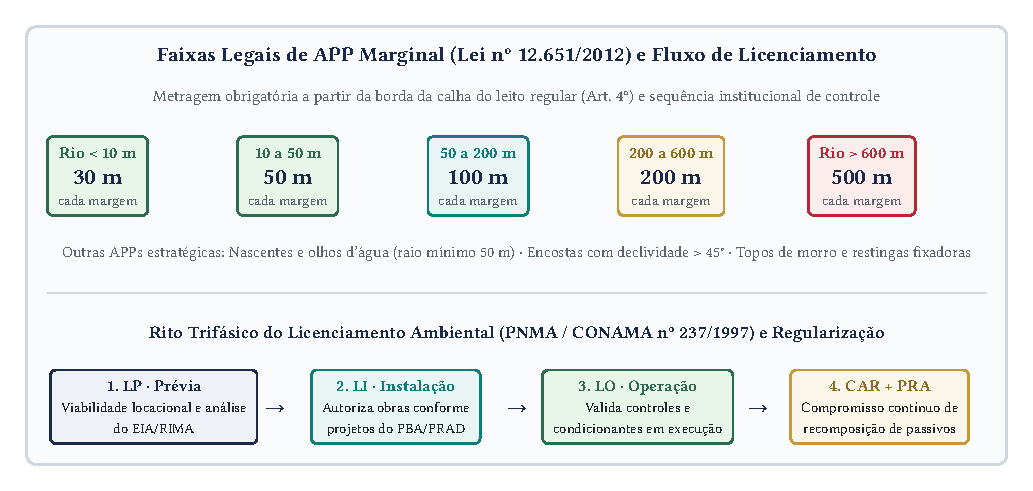
\includegraphics[width=0.95\textwidth]{figures/fig_cap14_faixas_app_codigo_florestal.pdf}
  \caption{Escalonamento das faixas legais de APP marginal conforme a largura do curso d'água (Lei n\textsuperscript{o} 12.651/2012) e articulação com o rito trifásico de licenciamento e regularização (CAR e PRA).}
  \label{fig:faixas_app_codigo_florestal}
\end{figure}

\subsection{Reserva Legal (Art. 12), CAR e PRA}

A \textbf{Reserva Legal (RL)} corresponde à área localizada no interior de uma propriedade ou posse rural que deve ser mantida com cobertura de vegetação nativa, permitindo o manejo sustentável mediante plano aprovado. Os percentuais mínimos exigidos sobre a área total do imóvel variam conforme o bioma e a região. Na Amazônia Legal, exigem-se \textbf{$80\%$} para imóveis situados em áreas de \textbf{florestas}, \textbf{$35\%$} em áreas de \textbf{cerrado} e \textbf{$20\%$} em áreas de \textbf{campos gerais}; nos \textbf{demais biomas e regiões do país} (incluindo Caatinga, Mata Atlântica e Cerrado na Bahia), o percentual mínimo legal é de \textbf{$20\%$}.

O Art. 15 do Código Florestal admite o cômputo das APPs no cálculo do percentual da Reserva Legal apenas quando o benefício previsto mantiver preservadas as áreas existentes sem nova conversão para uso alternativo do solo, a área a ser computada estiver conservada ou em processo de recuperação e o proprietário houver efetuado a inscrição no \textbf{Cadastro Ambiental Rural (CAR)}. O CAR é o registro público eletrônico nacional obrigatório que reúne o perímetro georreferenciado do imóvel, suas APPs, RL, remanescentes de vegetação nativa e áreas consolidadas, servindo como porta de entrada para o \textbf{Programa de Regularização Ambiental (PRA)}, mediante assinatura de Termo de Compromisso para recomposição ou compensação de passivos.

\begin{boxFormula}[Cálculo Espacial de APPs e Reserva Legal em Imóvel Rural]
\begin{align}
  A_{\text{marg}} &= \frac{n_m \cdot L \cdot w}{10.000} \qquad\qquad A_{\text{nasc}} = \frac{\pi \cdot r^2}{10.000} \qquad\qquad A_{\text{RL}} = f_{\text{bioma}} \cdot A_{\text{imóvel}}
\end{align}
Nessas expressões em hectares ($\text{ha}$), $A_{\text{marg}}$ representa a área da APP marginal do curso d'água, em que $n_m \in \{1, 2\}$ indica se o rio margeia apenas um lado ($n_m = 1$) ou atravessa o imóvel com ambas as margens dentro da propriedade ($n_m = 2$), $L$ é a extensão longitudinal do rio ($\text{m}$) e $w$ corresponde à largura da faixa legal ($\text{m}$). Para nascentes perenes ($A_{\text{nasc}}$), o raio mínimo $r = 50\text{ m}$ resulta em $\approx 0{,}7854\text{ ha}$ por nascente isolada. Já $A_{\text{RL}}$ define a área mínima de Reserva Legal exigida para a área total $A_{\text{imóvel}}$, aplicando-se $f_{\text{bioma}} \in \{0{,}80;\, 0{,}35;\, 0{,}20\}$.
\end{boxFormula}

Na prática da Análise Ambiental, a espacialização conjunta das faixas marginais, nascentes, encostas íngremes, topos de morro e Reserva Legal sobre o imóvel rural compatibiliza as condicionantes cartográficas do CAR com as etapas do licenciamento ambiental trifásico (Figura~\ref{fig:licenciamento_apps}).

\begin{figure}[H]
  \centering
  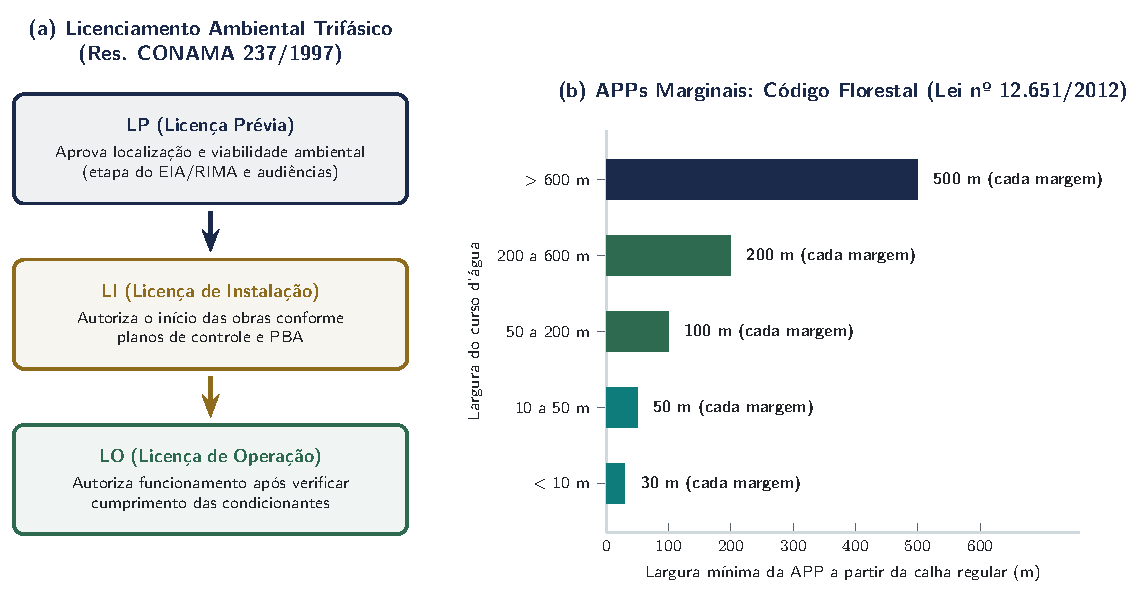
\includegraphics[width=0.95\textwidth]{figures/fig14_licenciamento_apps.pdf}
  \caption{Integração esquemática entre o rito do Licenciamento Ambiental Trifásico (LP, LI, LO) e a espacialização legal das Áreas de Preservação Permanente e Reserva Legal em imóvel rural.}
  \label{fig:licenciamento_apps}
\end{figure}

O Exemplo 14.1 aplica essas relações geométricas ao levantamento fundiário de uma propriedade rural situada na Caatinga baiana.

\begin{boxExemplo}{14.1 (Básico)}{Delimitação de APPs e Reserva Legal em Imóvel Rural na Bahia}
\passoEnunciado{Durante a análise ambiental de uma propriedade rural localizada no interior da Bahia (bioma Caatinga, fora da Amazônia Legal), necessita-se quantificar a área total de APP e a área mínima de Reserva Legal para conferência do CAR.}
\passoDados{Área total do imóvel $A_{\text{imóvel}} = 250{,}0\text{ ha}$; o imóvel é margeado em apenas um dos lados ($n_m = 1$) por um rio perene de $35\text{ m}$ de largura ao longo de $1.200\text{ m}$ de extensão; no interior da propriedade existe ainda $1$ nascente perene isolada (sem sobreposição espacial com a faixa do rio).}
\passoPedido{Calcule a área da APP marginal ($A_{\text{marg}}$), a área da APP de nascente ($A_{\text{nasc}}$), a área total de APP do imóvel e a área mínima exigida de Reserva Legal ($A_{\text{RL}}$).}
\passoMetodo{Aplicação dos parâmetros do Art. 4\textsuperscript{o} e Art. 12 da Lei n\textsuperscript{o} 12.651/2012 e conversão de $\text{m}^2$ para hectares ($1\text{ ha} = 10.000\text{ m}^2$).}
\passoContas{%
\textbf{Etapa 1, Largura legal ($w = 50\text{ m}$ para rio entre $10$ e $50\text{ m}$) e APP marginal ($n_m = 1$):}
\[
  A_{\text{marg}} = \frac{1 \times 1.200 \times 50}{10.000} = \frac{60.000}{10.000} = 6{,}00\text{ ha}
\]
\textbf{Etapa 2, APP da nascente ($r = 50\text{ m}$) e total de APP no imóvel:}
\[
  A_{\text{nasc}} = \frac{\pi \cdot 50^2}{10.000} \approx 0{,}79\text{ ha} \qquad\qquad A_{\text{APP}} = 6{,}00 + 0{,}79 = 6{,}79\text{ ha}
\]
\textbf{Etapa 3, Reserva Legal mínima exigida na Bahia ($f_{\text{bioma}} = 0{,}20$):}
\[
  A_{\text{RL}} = 0{,}20 \times 250{,}0 = 50{,}00\text{ ha}
\]}
\passoResposta{$A_{\text{marg}} = 6{,}00\text{ ha}$; $A_{\text{nasc}} = 0{,}79\text{ ha}$; $A_{\text{APP}} = 6{,}79\text{ ha}$; Reserva Legal mínima $A_{\text{RL}} = 50{,}00\text{ ha}$.}
\passoVerificacao{O rio de $35\text{ m}$ enquadra-se na faixa de $10\text{ m}$ a $50\text{ m}$ (APP de $50\text{ m}$), e a Bahia situa-se integralmente fora da Amazônia Legal, aplicando-se o percentual de $20\%$ de Reserva Legal.}
\end{boxExemplo}

Em cursos d'água intermitentes ou sazonais do Semiárido, a escolha da referência física correta na margem evita erros severos de subdimensionamento da faixa protegida.

\begin{boxErro}[Erro 2: Medir a APP Marginal a Partir do Espelho d'Água da Estiagem]
No Semiárido e em rios sazonais, o espelho d'água reduz-se drasticamente na seca ou desaparece nos trechos intermitentes. O Art. 4\textsuperscript{o} do Código Florestal determina que a faixa de APP seja medida a partir da \textbf{borda da calha do leito regular}, independentemente do nível reduzido do filete d'água na estação seca.
\end{boxErro}

Quando um imóvel apresenta déficit parcial de Reserva Legal fora de APP, o Art. 15 permite verificar se a vegetação nativa preservada nas APPs supre o percentual legal exigido (Exemplo 14.2).

\begin{boxExemplo}{14.2 (Intermediário)}{Verificação do Cômputo de APP na Reserva Legal (Art. 15 do Código Florestal)}
\passoEnunciado{Um imóvel rural de $400{,}0\text{ ha}$ situado em área de cerrado dentro da Amazônia Legal (percentual legal de Reserva Legal de $35\%$) busca regularização ambiental no CAR/PRA sem realizar novas supressões.}
\passoDados{Área total $= 400{,}0\text{ ha}$; percentual de RL exigido $= 35\%$; área de APP integralmente conservada $= 60{,}0\text{ ha}$; área de vegetação nativa conservada fora da APP $= 90{,}0\text{ ha}$. O proprietário manteve intacta a cobertura remanescente e inscreveu o imóvel no CAR.}
\passoPedido{Calcule a área de RL exigida, verifique o déficit existente sem cômputo da APP e avalie se o cômputo previsto no Art. 15 da Lei n\textsuperscript{o} 12.651/2012 regulariza o imóvel.}
\passoMetodo{Cálculo da RL exigida ($0{,}35 \cdot A_{\text{imóvel}}$) e soma condicionada da APP conservada à vegetação nativa remanescente.}
\passoContas{%
\textbf{Etapa 1, Reserva Legal exigida ($35\%$) e balanço sem cômputo da APP:}
\[
  A_{\text{RL, exigida}} = 0{,}35 \times 400{,}0 = 140{,}0\text{ ha} \qquad\qquad \text{Déficit} = 140{,}0 - 90{,}0 = 50{,}0\text{ ha}
\]
\textbf{Etapa 2, Balanço com cômputo da APP (Art. 15) e saldo excedente:}
\[
  A_{\text{RL, computada}} = 90{,}0 + 60{,}0 = 150{,}0\text{ ha} \quad (37{,}5\% > 35\%) \qquad \text{Excedente} = 150{,}0 - 140{,}0 = 10{,}0\text{ ha}
\]}
\passoResposta{Sem cômputo, haveria déficit de $50{,}0\text{ ha}$; aplicando o Art. 15, o imóvel soma $150{,}0\text{ ha}$ ($37{,}5\%$), cumprindo os $140{,}0\text{ ha}$ exigidos com $10{,}0\text{ ha}$ excedentes.}
\passoVerificacao{O cômputo da APP mantém a área sob proteção integral do Art. 4\textsuperscript{o} para preservação hídrica e edáfica, apenas contribuindo para o atingimento do percentual mínimo de RL quando cumpridas todas as exigências legais.}
\end{boxExemplo}

Diferenciar as regras de compensação da Reserva Legal das exigências estritas aplicáveis às APPs evita interpretações jurídicas inválidas em perícias e processos de regularização.

\begin{boxErro}[Erro 3: Confundir Recuperação de APP com Compensação em Outro Imóvel]
Enquanto o passivo de Reserva Legal pode ser compensado fora do imóvel (via Cota de Reserva Ambiental ou área equivalente no mesmo bioma), passivos em \textbf{Áreas de Preservação Permanente} exigem recomposição física \textit{in loco} na própria área protegida, pois sua função hidrogeomorfológica é intransferível.
\end{boxErro}

\section{PRAD e Tríplice Responsabilidade Ambiental}

O \textbf{Plano de Recuperação de Áreas Degradadas (PRAD)} é o instrumento técnico-executivo exigido tanto em processos de licenciamento e regularização (PRA) quanto em condenações administrativas ou judiciais para recompor funções ecológicas, hidrológicas e edáficas de áreas alteradas. Todo PRAD consistente precisa atuar sobre o processo causal da degradação, pois a revegetação de uma superfície onde a enxurrada continua se concentrando tende a fracassar nos primeiros ciclos chuvosos. Embora modelos simplificados variem entre órgãos (IBAMA, INEMA), a estrutura técnica completa de um PRAD articula cinco blocos sequenciais e interdependentes. O projeto inicia-se pela \textbf{identificação e caracterização da área}, reunindo delimitação cartográfica georreferenciada, histórico da degradação, diagnóstico de solo, relevo, drenagem e cobertura vegetal remanescente. Em seguida, executa-se o \textbf{isolamento dos fatores de degradação} mediante cercamento contra gado, controle de incêndios, fechamento de acessos clandestinos e eliminação de fontes de poluição.

Superada a fase de isolamento, passa-se ao \textbf{preparo físico e controle erosivo} com técnicas de bioengenharia, compreendendo reconformação de taludes, drenagem superficial, instalação de paliçadas, biomantas e correção física ou química do substrato. A etapa seguinte concentra-se na \textbf{recomposição vegetal}, definindo o método adequado (condução da regeneração natural, semeadura direta ou plantio de mudas em área total ou enriquecimento), a escolha de espécies nativas regionais distribuídas em grupos sucessionais (pioneiras de recobrimento e secundárias tardias de diversidade), o cálculo do número de mudas e a reserva técnica para replantio (Exemplo 14.3). Para assegurar a efetividade das ações, o PRAD encerra-se com um \textbf{cronograma e plano de monitoramento} de $24$ a $60$ meses apoiado em metas de execução (o que foi implantado) e metas ambientais verificáveis por indicadores objetivos, tais como taxa de sobrevivência de mudas, cobertura de copa, estabilização de sulcos e recuperação da qualidade do solo.

\begin{boxExemplo}{14.3 (Intermediário)}{Dimensionamento de Mudas e Grupos Ecológicos em PRAD}
\passoEnunciado{Para cumprir um Termo de Compromisso no PRA, elabora-se o PRAD de uma área degradada em APP de margem fluvial que será recuperada por plantio total de espécies nativas regionais.}
\passoDados{Área a recuperar $A = 4{,}50\text{ ha}$ ($45.000\text{ m}^2$); espaçamento adotado entre mudas de $3{,}0\text{ m} \times 2{,}0\text{ m}$ ($6{,}0\text{ m}^2$ por muda); composição florística composta por $60\%$ de espécies de recobrimento (pioneiras e secundárias iniciais) e $40\%$ de espécies de diversidade (secundárias tardias e clímax); reserva técnica de $15\%$ sobre o plantio inicial para replantio de falhas.}
\passoPedido{Calcule o número base de mudas para o plantio inicial, a quantidade destinada a cada grupo ecológico, a reserva de replantio e o total de mudas a adquirir no viveiro.}
\passoMetodo{Divisão da área total pela área útil por cova e repartição proporcional por grupo sucessional.}
\passoContas{%
\textbf{Etapa 1, Quantidade base de mudas e repartição por grupo ecológico:}
\begin{align*}
  N_{\text{base}} &= \frac{45.000}{6{,}0} = 7.500\text{ mudas} \\
  N_{\text{recobrimento}} &= 7.500 \times 0{,}60 = 4.500\text{ mudas} \qquad N_{\text{diversidade}} = 7.500 \times 0{,}40 = 3.000\text{ mudas}
\end{align*}
\textbf{Etapa 2, Reserva técnica de $15\%$ e total geral de mudas:}
\begin{align*}
  N_{\text{replantio}} &= 7.500 \times 0{,}15 = 1.125\text{ mudas} \\
  N_{\text{total}} &= 7.500 + 1.125 = 8.625\text{ mudas}
\end{align*}}
\passoResposta{Plantio inicial de $7.500$ mudas ($4.500$ de recobrimento e $3.000$ de diversidade), acrescido de $1.125$ mudas para replantio, totalizando $8.625$ mudas.}
\passoVerificacao{A densidade de $1.667\text{ mudas}\cdot\text{ha}^{-1}$ ($7.500 / 4{,}5$) corresponde exatamente ao padrão clássico de $3{,}0\text{ m} \times 2{,}0\text{ m}$ adotado em projetos de restauração florestal.}
\end{boxExemplo}

O descumprimento das normas ambientais submete o infrator (pessoa física ou jurídica) à \textbf{Tríplice Responsabilidade Ambiental}, consagrada no Art. 225, \S 3\textsuperscript{o} da Constituição Federal e regulamentada pela \textbf{Lei de Crimes Ambientais (Lei n\textsuperscript{o} 9.605/1998)} e pelo Decreto n\textsuperscript{o} 6.514/2008. Na esfera \textbf{civil}, a responsabilidade é \textbf{objetiva e \textit{propter rem}}, impondo a obrigação de reparar integralmente o dano ambiental ou indenizá-lo independentemente da comprovação de culpa ou dolo, bastando o nexo causal entre a atividade e o dano; além disso, a obrigação de recompor APP e RL acompanha o imóvel, transferindo-se ao sucessor em caso de venda. De forma independente e cumulativa, a esfera \textbf{administrativa} abrange sanções aplicadas pelo poder de polícia ambiental (IBAMA, INEMA, municípios), como advertência, multa simples ou diária, apreensão de equipamentos, embargo de obra ou atividade e suspensão de licenças, enquanto a esfera \textbf{penal} prevê penas privativas de liberdade, restritivas de direitos ou multa criminal a pessoas físicas e jurídicas por condutas tipificadas como crimes ambientais, a exemplo de desmatar APP sem autorização, poluir mananciais ou operar empreendimento potencialmente poluidor sem licença válida (Exemplo 14.4).

\begin{boxExemplo}{14.4 (Intermediário)}{Análise de Responsabilidade Administrativa e Civil por Supressão em APP}
\passoEnunciado{Durante vistoria fiscalizatória em uma propriedade rural, constatou-se o desmatamento não autorizado de vegetação nativa em APP marginal para implantação de pastagem.}
\passoDados{Área suprimida irregularmente $= 3{,}60\text{ ha}$; valor-base didático de multa administrativa adotado no exercício $= \reais{5.000{,}00}\cdot\text{ha}^{-1}$, acrescido de $50\%$ por incidir especificamente em APP; custo unitário estimado de execução e monitoramento de PRAD por $3$ anos $= \reais{18.000{,}00}\cdot\text{ha}^{-1}$.}
\passoPedido{Calcule o valor da multa administrativa, o custo da reparação civil via PRAD e o desembolso financeiro total estimado, explicando a relação com a esfera penal.}
\passoMetodo{Aplicação independente das esferas administrativa e civil segundo o princípio da Tríplice Responsabilidade Ambiental (Art. 225, \S 3\textsuperscript{o} da CF/88 e Lei n\textsuperscript{o} 9.605/1998).}
\passoContas{%
\textbf{Etapa 1, Multa administrativa com acréscimo de $50\%$ e custo do PRAD (esfera civil):}
\[
  M_{\text{adm}} = 3{,}60 \times 5.000{,}00 \times 1{,}50 = \reais{27.000{,}00} \qquad\qquad C_{\text{PRAD}} = 3{,}60 \times 18.000{,}00 = \reais{64.800{,}00}
\]
\textbf{Etapa 2, Desembolso financeiro total nas duas esferas:}
\[
  C_{\text{total}} = 27.000{,}00 + 64.800{,}00 = \reais{91.800{,}00}
\]}
\passoResposta{Multa administrativa de $\reais{27.000{,}00}$ e custo de PRAD de $\reais{64.800{,}00}$, somando $\reais{91.800{,}00}$, sem prejuízo da eventual responsabilização penal (Art. 38 da Lei n\textsuperscript{o} 9.605/1998).}
\passoVerificacao{O pagamento da multa administrativa mantém íntegra a obrigação civil de recuperar a APP, pois as três esferas atuam de forma independente e cumulativa.}
\end{boxExemplo}

\etapa{4}{Síntese Aplicada: Auditoria de Prazos e Etapas no Licenciamento Trifásico}

A articulação entre conformidade jurídica, execução física de programas ambientais (como PRADs e medidas de bioengenharia) e validade das licenças exige controle rigoroso de prazos administrativos. O Exemplo 14.5 sintetiza a auditoria do rito trifásico e a contagem legal para renovação da Licença de Operação junto ao INEMA.

\begin{boxExemplo}{14.5 (Avançado)}{Auditoria de Prazos e Etapas no Licenciamento Ambiental Trifásico}
\passoEnunciado{Um empreendimento energético de médio impacto ambiental na Bahia obteve sua Licença de Operação (LO) junto ao órgão estadual competente (INEMA) após cumprir o rito trifásico.}
\passoDados{Data de emissão da LO igual a $10/08/2026$; prazo de validade concedido na LO igual a $6$ anos (vencimento em $10/08/2032$).}
\passoPedido{Indique as atividades permitidas em cada fase anterior (LP e LI), verifique se o prazo de $6$ anos está dentro do intervalo legal da LO e determine a data limite para protocolar o pedido de renovação da LO com prorrogação automática.}
\passoMetodo{Confronto com os limites da Resolução CONAMA n\textsuperscript{o} 237/1997 (Art. 18) e da Lei Complementar n\textsuperscript{o} 140/2011 (Art. 14, \S 4\textsuperscript{o}).}
\passoContas{%
\textbf{Etapa 1, Verificação do prazo legal da LO:} a legislação fixa o intervalo de $4$ a $10$ anos para a LO, logo a validade de $6$ anos enquadra-se na faixa permitida.

\textbf{Etapa 2, Contagem regressiva dos $120$ dias para protocolo de renovação:} partindo de $10/08/2032$, subtraem-se $10$ dias de agosto (restam $110$ dias), $31$ dias de julho (restam $79$ dias), $30$ dias de junho (restam $49$ dias) e $31$ dias de maio (restam $18$ dias). Em abril ($30$ dias), alcança-se $30 - 18 = 12$, fixando a data limite em \textbf{12/04/2032}.}
\passoResposta{A LP aprova apenas concepção e localização e a LI autoriza a obra; o prazo de $6$ anos da LO é válido ($4$ a $10$ anos); o pedido de renovação deve ser protocolado até \textbf{12/04/2032} para garantir a prorrogação automática.}
\passoVerificacao{Caso o empreendedor protocole após o prazo de $120$ dias e a licença vença sem análise, a operação torna-se irregular, sujeitando o responsável a embargo e autuação.}
\end{boxExemplo}

\etapa{5}{Armadilha Conceitual e Materiais Audiovisuais de Apoio}

Mesmo quando um empreendimento ou propriedade cumpre uma sanção administrativa imediata, a obrigação de reparar integralmente o passivo ambiental permanece exigível pelas demais esferas jurídicas.

\begin{boxErro}[Erro 4: Tratar a Tríplice Responsabilidade como Alternativa (``Paga Multa ou Recupera'')]
Um equívoco frequente é supor que o pagamento de multa administrativa encerra o problema ambiental. Na realidade, as esferas civil, administrativa e penal são independentes, de modo que o infrator paga a multa (administrativa), continua obrigado a recuperar integralmente a área via PRAD (civil) e pode responder a processo criminal (penal).
\end{boxErro}

Para aprofundar o entendimento sobre a Política Nacional do Meio Ambiente, o Código Florestal e o arcabouço normativo brasileiro, assista às videoaulas selecionadas na página da disciplina, iniciando por \textit{Gestão Ambiental - Legislação e Certificação Ambiental} (\url{https://www.youtube.com/watch?v=L-WEcC2IlbA}), prosseguindo com \textit{Direito Ambiental: Código Florestal} (\url{https://www.youtube.com/watch?v=ApidLjWC4Dc}) e concluindo com \textit{Legislação Ambiental Brasileira} (\url{https://www.youtube.com/watch?v=gC4uHPJDiVA}).

\etapa{6}{Exercícios de Fixação (15 Questões)}

\subsection*{Bloco A: Questões Conceituais Básicas (1 a 5)}
\begin{enumerate}[leftmargin=1.8em, itemsep=6pt]
  \item Cite os objetivos principais da Política Nacional do Meio Ambiente (Lei n\textsuperscript{o} 6.938/1981) e explique a função do CONAMA e dos órgãos executores/seccionais (IBAMA e INEMA) dentro do SISNAMA.
  \espacoResolucao[1.8cm]

  \item Diferencie o escopo técnico e jurídico da Licença Prévia (LP), da Licença de Instalação (LI) e da Licença de Operação (LO).
  \espacoResolucao[1.8cm]

  \item Explique a diferença entre o EIA (Estudo de Impacto Ambiental) e o RIMA (Relatório de Impacto Ambiental), indicando em qual etapa do licenciamento são analisados.
  \espacoResolucao[1.8cm]

  \item Distinga a função ambiental e o regime jurídico da Área de Preservação Permanente (APP) em relação à Reserva Legal (RL) no Código Florestal.
  \espacoResolucao[1.8cm]

  \item Descreva os cinco blocos técnicos mínimos que estruturam um Plano de Recuperação de Áreas Degradadas (PRAD).
  \espacoResolucao[1.8cm]
\end{enumerate}

\subsection*{Bloco B: Questões Intermediárias e Quantitativas (6 a 10)}
\begin{enumerate}[leftmargin=1.8em, itemsep=6pt, start=6]
  \item Uma propriedade rural de $180{,}0\text{ ha}$ na Bahia é atravessada por um riacho de $6{,}0\text{ m}$ de largura média (ambas as margens no interior do imóvel, $n_m = 2$) ao longo de $800\text{ m}$ de extensão, possuindo ainda $2$ nascentes perenes isoladas. Calcule a área total de APP do imóvel e a área mínima exigida de Reserva Legal.
  \espacoResolucao[2.1cm]

  \item Um imóvel de $500{,}0\text{ ha}$ situado em área de floresta na Amazônia Legal possui $310{,}0\text{ ha}$ de vegetação nativa fora de APP e $100{,}0\text{ ha}$ de APP conservada. Determine a RL exigida ($80\%$), verifique se há déficit sem o cômputo da APP e avalie se o cômputo do Art. 15 supre integralmente a exigência legal.
  \espacoResolucao[2.1cm]

  \item Para recuperar uma área alterada de $3{,}00\text{ ha}$ ($30.000\text{ m}^2$) em APP, um PRAD especifica plantio de mudas nativas no espaçamento $2{,}5\text{ m} \times 2{,}0\text{ m}$ ($5{,}0\text{ m}^2$ por muda), com $50\%$ de pioneiras/secundárias iniciais e $50\%$ de secundárias tardias/clímax, além de $10\%$ de reserva para replantio. Calcule o total de mudas a adquirir.
  \espacoResolucao[2.1cm]

  \item Uma indústria recebeu sua Licença de Instalação (LI) com validade de $4$ anos e, após concluir a obra, obteve a LO em $15/05/2027$ com validade de $5$ anos. Indique a data de vencimento da LO e a data limite para protocolar o pedido de renovação com antecedência mínima de $120$ dias.
  \espacoResolucao[2.1cm]

  \item Um empreendimento suprimiu irregularmente $2{,}50\text{ ha}$ de vegetação nativa fora de APP, sofrendo multa didática de $\reais{4.000{,}00}\cdot\text{ha}^{-1}$ e obrigação de executar PRAD orçado em $\reais{14.000{,}00}\cdot\text{ha}^{-1}$. Calcule o custo total nas esferas administrativa e civil.
  \espacoResolucao[2.1cm]
\end{enumerate}

\subsection*{Bloco C: Questões Objetivas de Múltipla Escolha (11 a 15)}
\begin{enumerate}[leftmargin=1.8em, itemsep=6pt, start=11]
  \item No âmbito do SISNAMA (Lei n\textsuperscript{o} 6.938/1981), o órgão consultivo e deliberativo responsável por estabelecer normas e padrões ambientais nacionais mediante resoluções é o:
  \begin{alternativas}
    \item IBAMA.
    \item CONAMA.
    \item INEMA.
    \item ICMBio.
    \item Ministério Público Federal.
  \end{alternativas}
  \espacoResolucao[1.2cm]

  \item De acordo com a Lei n\textsuperscript{o} 12.651/2012 (Art. 4\textsuperscript{o}), a faixa mínima de Área de Preservação Permanente para um curso d'água natural com $75\text{ m}$ de largura de calha regular e para uma nascente perene são, respectivamente:
  \begin{alternativas}
    \item $50\text{ m}$ e $30\text{ m}$.
    \item $100\text{ m}$ e $50\text{ m}$.
    \item $200\text{ m}$ e $50\text{ m}$.
    \item $100\text{ m}$ e $100\text{ m}$.
    \item $30\text{ m}$ e $50\text{ m}$.
  \end{alternativas}
  \espacoResolucao[1.2cm]

  \item Os percentuais mínimos de Reserva Legal exigidos pelo Código Florestal para imóveis situados na Amazônia Legal em áreas de floresta, cerrado e campos gerais são, respectivamente:
  \begin{alternativas}
    \item $80\%$, $35\%$ e $20\%$.
    \item $80\%$, $50\%$ e $20\%$.
    \item $50\%$, $35\%$ e $20\%$.
    \item $80\%$, $20\%$ e $20\%$.
    \item $35\%$, $20\%$ e $20\%$.
  \end{alternativas}
  \espacoResolucao[1.2cm]

  \item Sobre a Tríplice Responsabilidade Ambiental no ordenamento jurídico brasileiro, é correto afirmar que:
  \begin{alternativas}
    \item A responsabilidade civil ambiental é subjetiva, exigindo sempre a prova de intenção dolosa do degradador.
    \item O pagamento da multa administrativa extingue automaticamente a obrigação de reparar o dano em PRAD.
    \item As sanções administrativas, civis e penais podem incidir cumulativamente sobre o mesmo fato danoso, sendo objetiva a obrigação civil de reparar o dano.
    \item Pessoas jurídicas não podem ser responsabilizadas na esfera penal por crimes ambientais no Brasil.
    \item A obrigação de recompor a Reserva Legal desaparece quando o imóvel rural é vendido a terceiros.
  \end{alternativas}
  \espacoResolucao[1.2cm]

  \item No Licenciamento Ambiental Trifásico (Resolução CONAMA n\textsuperscript{o} 237/1997), a licença que autoriza o início efetivo das obras civis e da instalação dos equipamentos, mediante atendimento às condicionantes da fase preliminar, é a:
  \begin{alternativas}
    \item Licença Prévia (LP).
    \item Licença de Instalação (LI).
    \item Licença de Operação (LO).
    \item Outorga Preventiva de Uso da Água.
    \item Certidão de Cadastro Ambiental Rural (CAR).
  \end{alternativas}
  \espacoResolucao[1.2cm]
\end{enumerate}

\etapa{7}{Questões no Estilo ENADE e Concursos Ambientais}

\begin{boxDica}[Foco de Provas, ENADE e Concursos (IBAMA / INEMA / Perícia)]
Questões de concursos e do ENADE frequentemente apresentam situações reais de campo em que um proprietário ou empreendedor confunde fases do licenciamento, mede APPs de forma equivocada ou tenta compensar APP fora do imóvel. Domine os números exatos da Lei n\textsuperscript{o} 12.651/2012 e a independência das três esferas de responsabilidade.
\end{boxDica}

\begin{enumerate}[leftmargin=1.8em, itemsep=7pt]
  \item \textbf{[Questão Autoral, Estilo ENADE / Geografia]} Durante visita técnica a uma propriedade rural localizada no Semiárido Baiano, estudantes da disciplina Análise Ambiental observaram que um trecho de $600\text{ m}$ da margem de um rio perene de $15\text{ m}$ de largura encontrava-se desmatado e com sulcos erosivos ativos. O proprietário afirmou que não havia necessidade de recomposição porque: (1) a faixa desmatada media $30\text{ m}$ de largura a partir do espelho d'água atual na estação seca; e (2) ele pretendia comprar uma área de Caatinga preservada em outro município para ``compensar a APP'' desmatada. À luz da Lei n\textsuperscript{o} 12.651/2012, avalie as afirmações:
  \begin{itemize}[leftmargin=1.4em, itemsep=2pt]
    \item[I.] Para um curso d'água de $15\text{ m}$ de largura, a APP marginal mínima é de $50\text{ m}$ medidos a partir da borda da calha do leito regular, excluído o espelho d'água da estiagem.
    \item[II.] A compensação em outro imóvel rural aplica-se a déficits de Reserva Legal, não substituindo a obrigação de recompor fisicamente a APP degradada no próprio imóvel.
    \item[III.] Por se tratar de propriedade situada na Bahia, o percentual mínimo de Reserva Legal exigido é de $35\%$.
  \end{itemize}
  É correto o que se afirma em:
  \begin{alternativas}
    \item I, apenas.
    \item III, apenas.
    \item I e II, apenas.
    \item II e III, apenas.
    \item I, II e III.
  \end{alternativas}

  \item \textbf{[Questão Autoral, Estilo Concurso Analista Ambiental / INEMA-BA]} Um empreendimento com potencial de significativa degradação ambiental protocolou pedido de licenciamento junto ao órgão estadual competente. Considerando a Resolução CONAMA n\textsuperscript{o} 001/1986 e a Resolução CONAMA n\textsuperscript{o} 237/1997, assinale a sequência correta de procedimentos administrativos:
  \begin{alternativas}
    \item Emissão da LI para abertura do canteiro de obras $\rightarrow$ elaboração do EIA/RIMA durante a operação $\rightarrow$ emissão da LP ao final da vida útil.
    \item Elaboração do EIA/RIMA e realização de audiência pública $\rightarrow$ análise e emissão da LP (viabilidade locacional) $\rightarrow$ aprovação dos projetos executivos e emissão da LI (autorização de obras) $\rightarrow$ verificação das condicionantes e emissão da LO (funcionamento).
    \item Inscrição no CAR $\rightarrow$ dispensa de LP e LI $\rightarrow$ emissão direta da LO por autodeclaração.
    \item Emissão simultânea de LP, LI e LO sem vistoria prévia para qualquer obra energética de grande porte.
    \item Elaboração apenas do RIMA simplificado sem EIA técnico, sendo facultativa a apresentação de alternativas locacionais.
  \end{alternativas}

  \item \textbf{[Questão Autoral, Estilo Concurso Analista Ambiental / IBAMA]} Em razão de vazamento de efluentes industriais não licenciados que provocou mortandade de peixes e contaminação de margem fluvial, o órgão ambiental lavrou auto de infração com multa, o Ministério Público ajuizou ação civil pública exigindo PRAD e indenização, e foi instaurado processo criminal com base na Lei n\textsuperscript{o} 9.605/1998. A defesa da empresa alegou que não houve intenção de poluir e que o pagamento da multa administrativa já impediria outras cobranças. Sob o ponto de vista jurídico-ambiental brasileiro, a tese da defesa é:
  \begin{alternativas}
    \item Procedente, pois a responsabilidade civil ambiental exige comprovação de dolo específico.
    \item Procedente, pois o princípio da unicidade impede a cumulação de multa administrativa com ação penal.
    \item Improcedente, pois a responsabilidade civil ambiental é objetiva (independe de culpa ou dolo) e as esferas civil, administrativa e penal são independentes e cumulativas.
    \item Parcialmente procedente, pois empresas privadas não podem sofrer sanções administrativas, apenas pessoas físicas.
    \item Improcedente apenas quanto à multa, mas procedente quanto ao PRAD, que é sempre facultativo em áreas industriais.
  \end{alternativas}
\end{enumerate}

\clearpage
\etapa{8}{Gabarito Comentado do Capítulo 14}

\begin{boxGabarito}[Resoluções Completas: Exercícios de Fixação (1 a 15)]
\begin{enumerate}[leftmargin=1.6em, itemsep=4pt]
  \item A PNMA visa preservar, melhorar e recuperar a qualidade ambiental propícia à vida e ao desenvolvimento sustentável. No SISNAMA, o \textbf{CONAMA} atua como órgão consultivo e deliberativo (editando normas e resoluções), enquanto \textbf{IBAMA} (federal) e \textbf{INEMA} (estadual na Bahia) executam o licenciamento, a fiscalização e o controle ambiental em suas respectivas esferas de competência.
  \item \textbf{LP:} atesta viabilidade ambiental e aprova localização/concepção (sem autorizar obra). \textbf{LI:} autoriza a instalação e construção do empreendimento segundo projetos executivos aprovados. \textbf{LO:} autoriza o início da operação após verificação do cumprimento das condicionantes anteriores.
  \item O \textbf{EIA} é o estudo técnico-científico multidisciplinar completo (diagnóstico, prognóstico, impactos, alternativas e programas); o \textbf{RIMA} é sua síntese acessível ao público e aos conselhos. Ambos integram a fase preliminar de avaliação que subsidia a decisão sobre a \textbf{LP}.
  \item A \textbf{APP} tem função ambiental rígida vinculada a feições sensíveis (rios, nascentes, encostas, topos de morro), exigindo preservação integral e recuperação \textit{in loco} quando degradada. A \textbf{Reserva Legal} é um percentual da área do imóvel rural ($20\%$, $35\%$ ou $80\%$) destinado à conservação da vegetação nativa com possibilidade de manejo sustentável e compensação legal em caso de passivo consolidado.
  \item Os cinco blocos são: (1) identificação e diagnóstico da área; (2) isolamento dos fatores de degradação; (3) preparo físico e obras de controle erosivo/bioengenharia; (4) recomposição vegetal estratificada; (5) cronograma executivo e monitoramento por indicadores.
  \item \textbf{Desenvolvimento:}
  Riacho de $6{,}0\text{ m}$ ($< 10\text{ m}$): APP de $w = 30\text{ m}$ em cada margem ($n_m = 2$).
  APP marginal: $A_{\text{marg}} = (2 \times 800 \times 30) / 10.000 = 48.000 / 10.000 = 4{,}80\text{ ha}$.
  APP das $2$ nascentes ($r = 50\text{ m}$): $A_{\text{nasc}} = 2 \times (\pi \cdot 50^2 / 10.000) \approx 2 \times 0{,}7854 = 1{,}57\text{ ha}$.
  APP total: $4{,}80 + 1{,}57 = \mathbf{6{,}37\text{ ha}}$.
  Reserva Legal mínima na Bahia ($20\%$): $A_{\text{RL}} = 0{,}20 \times 180{,}0 = \mathbf{36{,}00\text{ ha}}$.
  \item \textbf{Desenvolvimento:}
  RL exigida ($80\%$ em floresta na Amazônia Legal): $0{,}80 \times 500{,}0 = \mathbf{400{,}0\text{ ha}}$.
  Sem cômputo da APP: déficit de $400{,}0 - 310{,}0 = \mathbf{90{,}0\text{ ha}}$.
  Com cômputo da APP (Art. 15): $310{,}0 + 100{,}0 = \mathbf{410{,}0\text{ ha}}$ ($82{,}0\% > 80\%$), suprindo integralmente a exigência com $10{,}0\text{ ha}$ excedentes.
  \item \textbf{Desenvolvimento:}
  Mudas base: $30.000 / 5{,}0 = 6.000$ mudas ($3.000$ pioneiras/secundárias iniciais e $3.000$ secundárias tardias/clímax).
  Reserva de replantio ($10\%$): $6.000 \times 0{,}10 = 600$ mudas.
  Total a adquirir: $6.000 + 600 = \mathbf{6.600\text{ mudas}}$.
  \item \textbf{Desenvolvimento:}
  Vencimento da LO: \textbf{15/05/2032} ($5$ anos após $15/05/2027$).
  Contagem regressiva de $120$ dias (lembrando que 2032 é ano bissexto, mas fevereiro já ficou antes da contagem):
  Maio ($15$ dias: $01$ a $15/05$, restam $105$); Abril ($30$ dias, restam $75$); Março ($31$ dias, restam $44$); Fevereiro de 2032 ($29$ dias, restam $15$); Janeiro ($31 - 15 = 16 \rightarrow$ \textbf{16/01/2032}). (Em anos convencionais seria 15/01; em 2032, bissexto, $16/01/2032$ completa exatamente $120$ dias até $15/05/2032$.)
  \item \textbf{Desenvolvimento:}
  Multa administrativa: $2{,}50 \times 4.000{,}00 = \reais{10.000{,}00}$.
  Custo do PRAD (esfera civil): $2{,}50 \times 14.000{,}00 = \reais{35.000{,}00}$.
  Total nas duas esferas: $10.000{,}00 + 35.000{,}00 = \mathbf{\reais{45.000{,}00}}$.
  \item \textbf{Gabarito: (B).} O CONAMA é o órgão consultivo e deliberativo do SISNAMA.
  \item \textbf{Gabarito: (B).} Cursos d'água entre $50\text{ m}$ e $200\text{ m}$ de largura exigem $100\text{ m}$ de APP marginal; nascentes perenes exigem raio de $50\text{ m}$.
  \item \textbf{Gabarito: (A).} Art. 12 da Lei n\textsuperscript{o} 12.651/2012: $80\%$ (florestas), $35\%$ (cerrado) e $20\%$ (campos gerais) na Amazônia Legal.
  \item \textbf{Gabarito: (C).} A responsabilidade civil ambiental é objetiva (baseada no risco integral e no nexo causal) e coexiste de forma independente com as sanções administrativas e penais.
  \item \textbf{Gabarito: (B).} A Licença de Instalação (LI) é o ato administrativo que autoriza a execução física das obras e a instalação do empreendimento.
\end{enumerate}
\end{boxGabarito}

\begin{boxGabarito}[Resoluções Completas: Questões ENADE e Concursos (1 a 3)]
\begin{enumerate}[leftmargin=1.6em, itemsep=4pt]
  \item \textbf{Gabarito: (C).} As afirmações I e II estão corretas: rio de $15\text{ m}$ exige $50\text{ m}$ de APP medidos da borda da calha regular, e APP degradada deve ser recuperada no local, sem possibilidade de compensação externa. A afirmação III é falsa porque a Bahia está fora da Amazônia Legal, aplicando-se $20\%$ de Reserva Legal.
  \item \textbf{Gabarito: (B).} Apenas (B) respeita a ordem cronológica e legal do licenciamento trifásico para obras sujeitas a EIA/RIMA: estudos e audiência pública prévios à LP, projetos executivos e autorização de obras na LI, e funcionamento autorizado na LO.
  \item \textbf{Gabarito: (C).} A tese da defesa é improcedente em ambos os pontos: no Brasil, a obrigação civil de reparar o dano ambiental é objetiva (dispensa prova de dolo ou culpa) e as três esferas (civil, administrativa e penal) atuam de forma independente e cumulativa.
\end{enumerate}
\end{boxGabarito}

\begin{boxResumo}
\begin{itemize}[leftmargin=1.4em, itemsep=2.5pt]
  \item \textbf{PNMA (Lei n\textsuperscript{o} 6.938/1981):} institui o SISNAMA (CONAMA, MMA, IBAMA, ICMBio, órgãos estaduais como INEMA e órgãos municipais) e instrumentos como AIA, licenciamento, zoneamento e SINIMA.
  \item \textbf{Licenciamento Trifásico (CONAMA 237/1997 e 001/1986):} LP (viabilidade e localização; até $5$ anos), LI (instalação e obras; até $6$ anos) e LO (operação; $4$ a $10$ anos, renovação com $120$ dias de antecedência); EIA/RIMA obrigatório para significativa degradação.
  \item \textbf{Código Florestal (Lei n\textsuperscript{o} 12.651/2012):} APPs marginais de $30\text{ m}$ a $500\text{ m}$, nascentes de $50\text{ m}$, encostas $> 45^\circ$, topos de morro, restingas e manguezais; Reserva Legal de $80\%$, $35\%$ ou $20\%$; regularização via CAR e PRA.
  \item \textbf{PRAD e Tríplice Responsabilidade:} recomposição técnica com isolamento, bioengenharia, plantio estratificado e monitoramento; responsabilização civil objetiva, administrativa e penal cumulativas (Lei n\textsuperscript{o} 9.605/1998).
\end{itemize}
\end{boxResumo}

\begin{boxTeste}
Avalie cada afirmação com \textbf{V} (Verdadeiro) ou \textbf{F} (Falso) antes de conferir o gabarito abaixo:
\begin{enumerate}[leftmargin=1.6em, itemsep=3pt]
  \item ( \quad ) A Licença Prévia (LP) autoriza o empreendedor a realizar a supressão vegetal e a terraplenagem inicial do terreno enquanto conclui os projetos executivos para a LI.
  \item ( \quad ) Em um curso d'água natural de $40\text{ m}$ de largura, a APP marginal mínima prevista no Código Florestal é de $50\text{ m}$ em cada margem a partir da borda da calha do leito regular.
  \item ( \quad ) Na Bahia, o percentual mínimo de Reserva Legal exigido para imóveis rurais é de $20\%$, podendo a APP conservada ser computada apenas quando atendidos os requisitos cumulativos do Art. 15 da Lei n\textsuperscript{o} 12.651/2012.
  \item ( \quad ) A obrigação civil de reparar o dano ambiental independe da comprovação de dolo ou culpa do agente, coexistindo com eventuais multas administrativas e sanções penais.
\end{enumerate}
\vspace{4pt}
{\footnotesize\textbf{Gabarito do Checkpoint:} 1-\F\ (a instalação e a supressão dependem da LI) \quad|\quad 2-\V \quad|\quad 3-\V \quad|\quad 4-\V.}
\end{boxTeste}

\chapter{Manual Prático do Diagnóstico Ambiental Aplicado e Produtos Técnicos}
\label{cap:diagnostico_final_pratico}

\noindent\tagPratica
\vspace{4pt}

\begin{capObjetivos}
Ao concluir este capítulo, você será capaz de:
\begin{itemize}[leftmargin=1.5em, itemsep=2.5pt]
  \item Delimitar com rigor geográfico e cartográfico o recorte espacial do \textbf{Trabalho Prático Final} (Semana 16 do Plano CHF662, correspondente a $50\%$ da nota semestral), selecionando microbacia, encosta, margem fluvial, Área de Preservação Permanente (APP) ou área degradada compatível com a escala de análise (IBGE, 2018; Cavalcanti, 2006).
  \item Levantar, compatibilizar em ambiente SIG (QGIS) e validar bases cartográficas e dados abertos oficiais (MapBiomas, SRTM/TOPODATA, SICAR/CAR, IBGE e INEMA/SEI-BA) sob o sistema de referência geodésico oficial \textbf{SIRGAS 2000}.
  \item Integrar a caracterização físico-biótica e socioespacial ao mapeamento de processos de degradação e à montagem da \textbf{Matriz de Indicadores} (combinando o modelo PEIR, a qualidade do solo e a fragilidade ambiental de Ross).
  \item Calcular o \textbf{Índice Composto de Priorização de Intervenção ($IPI$)} para hierarquizar setores críticos e dimensionar propostas preliminares de conservação, bioengenharia e PRAD (Vital et al., 2020).
  \item Elaborar os produtos técnicos exigidos (mapas temáticos com elementos cartográficos obrigatórios e relatório técnico interpretativo) e auditar o trabalho pelo \textbf{Checklist de Entrega e Rubrica de Avaliação} ($5{,}0$ pontos) antes da socialização na Semana 16.
\end{itemize}
\end{capObjetivos}

\begin{capRevisao}
Este capítulo integra todos os módulos da disciplina CHF662 em um roteiro único de execução profissional:
\begin{itemize}[leftmargin=1.5em, itemsep=2.5pt]
  \item \textbf{Fundamentos e AIA (Módulos 1 e 2):} a distinção entre atividade, aspecto e impacto ambiental (Sánchez, 2013), o olhar socioambiental (Mendonça, 2001) e a articulação entre escalas espaciais e temporais orientam o recorte do diagnóstico.
  \item \textbf{Bacia, Morfopedologia e Ross (Módulo 3):} a microbacia hidrográfica (Capítulos 7 e 8) e os graus de Fragilidade Potencial e Emergente (Ross, 1994, Capítulo 9) formam a base territorial do mapeamento.
  \item \textbf{Indicadores, Solo e Degradação (Módulo 4):} o modelo PEIR (Capítulo 10), o Índice de Qualidade do Solo ($IQS$, Capítulo 11) e o diagnóstico de erosão linear e USLE (Capítulo 12) fornecem as métricas auditáveis.
  \item \textbf{Bioengenharia, Legislação e PRAD (Capítulos 13 e 14):} as técnicas de estabilização vegetativa e estrutural leve, o Código Florestal (Lei nº 12.651/2012) e as diretrizes do PRAD convertem o diagnóstico em proposta técnica exequível.
\end{itemize}
\end{capRevisao}

\etapa{3}{Guia Operacional do Trabalho Prático Final (Semana 16: 5,0 Pontos)}

\begin{boxSimbolo}[Vocabulário Técnico e Símbolos do Capítulo 15]
Para padronizar a comunicação técnica do Trabalho Prático Final, o \textbf{Recorte Espacial ($A_{\text{rec}}$)} designa a unidade territorial delimitada para o diagnóstico, correspondendo preferencialmente a uma microbacia hidrográfica, sub-bacia, vertente completa ou trecho de APP e área degradada. Todos os projetos em QGIS e os mapas finais devem adotar o \textbf{SIRGAS 2000} (Sistema de Referência Geocêntrico para as Américas), datum geodésico oficial do Brasil. Na definição da escala cartográfica, $A_{\min}$ indica a \textbf{área mínima mapeável} no terreno correspondente a $4\text{ mm}^2$ no mapa impresso, calculada por $A_{\min} = 4 \times 10^{-6} \cdot E^2\text{ m}^2$, em que $E$ é o denominador da escala $1:E$.

Na etapa de síntese quantitativa, a \textbf{Matriz de Indicadores} organiza os dados cruzando Pressão, Estado, Impacto e Resposta (PEIR) com atributos de qualidade do solo ($IQS$) e fragilidade emergente ($FE$). Desse cruzamento deriva-se o \textbf{Índice Composto de Priorização de Intervenção ($IPI$)}, parâmetro adimensional entre $0$ e $1$ empregado para ranquear setores críticos na alocação de bioengenharia e PRAD, enquanto $CE$ representa o \textbf{Custo-Efetividade} de uma intervenção, medido em $\text{t}\cdot\text{ano}^{-1}$ de sedimentos retidos por $\reais{1.000,00}$ investidos.
\end{boxSimbolo}

O Trabalho Prático Final da disciplina CHF662 representa $50\%$ da avaliação semestral ($5{,}0$ pontos) e simula a entrega de um diagnóstico técnico profissional em Análise Ambiental. O fluxo metodológico articula sete etapas encadeadas, partindo da delimitação espacial e do levantamento de bases abertas até a matriz de indicadores, os produtos cartográficos, a proposta de intervenção e a socialização dos resultados (Figura~\ref{fig:fluxo_diagnostico_final}).

\begin{figure}[H]
  \centering
  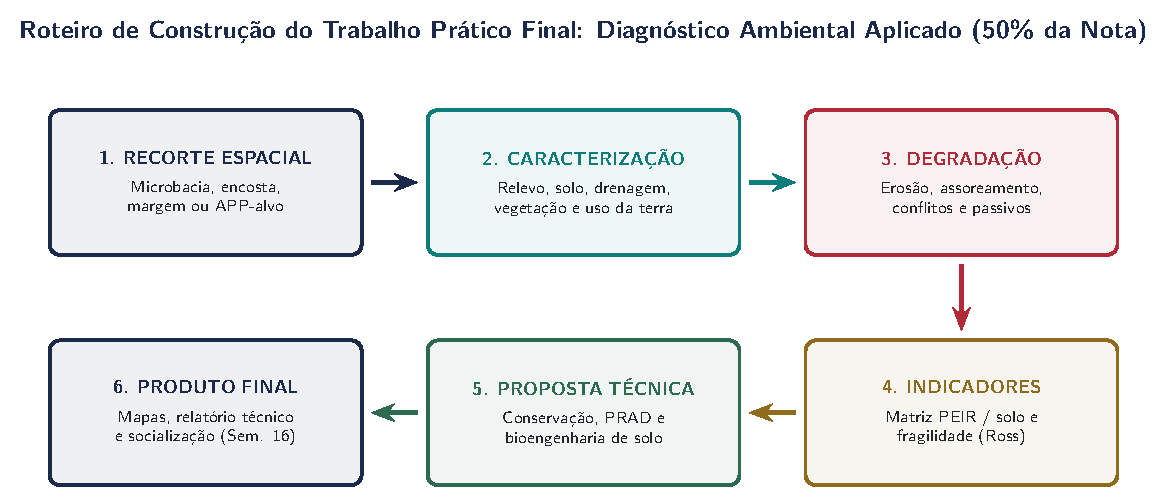
\includegraphics[width=0.94\textwidth]{figures/fig15_fluxo_diagnostico_final.pdf}
  \caption{Fluxograma operacional das sete etapas do Diagnóstico Ambiental Aplicado (Trabalho Prático Final da disciplina CHF662, Semana 16), integrando bases abertas, matriz de indicadores, produtos cartográficos e proposta de intervenção.}
  \label{fig:fluxo_diagnostico_final}
\end{figure}

\section{Etapa 1: Escolha e Delimitação do Recorte Espacial}

A escolha da área de estudo deve equilibrar \textbf{relevância socioambiental} e \textbf{viabilidade de levantamento} no prazo semestral (IBGE, 2018; Cavalcanti, 2006). Entre as possibilidades de recorte, a \textbf{microbacia hidrográfica} constitui a unidade preferencial por integrar divisores de água, rede de drenagem, conectividade hidrossedimentológica e uso da terra, recomendando-se áreas entre $1\text{ km}^2$ e $50\text{ km}^2$. Quando o foco recai sobre processos erosivos lineares (sulcos, ravinas e voçorocas) ou movimentos de massa em áreas urbanas e rurais, a delimitação pode concentrar-se em uma \textbf{encosta ou vertente representativa}. De modo complementar, diagnósticos voltados a passivo florestal (Lei nº 12.651/2012), assoreamento de açudes, antigas cascalheiras ou acessos de empreendimentos energéticos (como observado no campo do Semiárido) ajustam-se bem ao recorte de uma \textbf{margem de curso d'água, APP ou área degradada pontual}.

Qualquer que seja o recorte selecionado, a delimitação deve ser vetorizada em polígono fechado no QGIS (formato GeoPackage `.gpkg` ou Shapefile `.shp`), acompanhada de justificativa clara dos critérios naturais (divisores topográficos) ou legais e administrativos (limites de APP ou poligonal de empreendimento) adotados.

\section{Etapa 2: Levantamento de Bases Cartográficas e Dados Abertos}

Todo diagnóstico ambiental auditável depende de fontes públicas rastreáveis, organizadas em um banco geográfico padronizado em \textbf{SIRGAS 2000}, adotando-se coordenadas geográficas para contextualização regional e projeção UTM (fuso 24S para a maior parte da Bahia) nos cálculos de área e comprimento. As plataformas oficiais e suas aplicações diretas no trabalho final estão sistematizadas na Tabela~\ref{tab:bases_abertas_tpf}.

\begin{table}[H]
\centering
\caption{Principais bases cartográficas e dados abertos oficiais aplicados ao Trabalho Prático Final em CHF662.}
\label{tab:bases_abertas_tpf}
\renewcommand{\arraystretch}{1.20}
\small
\begin{tabularx}{\textwidth}{@{}p{2.9cm} p{3.8cm} >{\raggedright\arraybackslash}X@{}}
  \toprule
  \rowcolor{uefsNavy}
  \textcolor{white}{\bfseries Base / Plataforma} & \textcolor{white}{\bfseries Dados Extraídos} & \textcolor{white}{\bfseries Aplicação Direta no Trabalho Final} \\
  \midrule
  \textbf{IBGE} & Limites municipais, malha censitária, hidrografia e pedologia & Contextualização territorial, caracterização socioespacial e classes de solo. \\
  \rowcolor{bgGray}
  \textbf{SRTM / TOPODATA (INPE)} & Modelo Digital de Elevação ($30\text{ m}$), declividade e curvas de nível & Delimitação automática da microbacia, perfil de vertente, fator $LS$ e mapa clinográfico (Ross). \\
  \textbf{MapBiomas} & Séries anuais de uso e cobertura da terra ($30\text{ m}$) & Análise multitemporal (por exemplo, $1985\text{--}2024$), supressão de vegetação nativa e fator $C$ da USLE. \\
  \rowcolor{bgGray}
  \textbf{SICAR / CAR} & Perímetros de imóveis rurais, APPs e Reserva Legal declaradas & Verificação de passivo ambiental em APPs marginais e nascentes (Lei nº 12.651/2012). \\
  \textbf{INEMA / SEI-BA} & Outorgas, licenças ambientais, bacias estaduais e dados climáticos & Identificação de empreendimentos licenciados, conflitos hídricos e erosividade regional ($R$). \\
  \bottomrule
\end{tabularx}
\end{table}

Definidas as bases cartográficas de entrada, a equipe precisa compatibilizar a escala de apresentação dos mapas finais com o tamanho das feições erosivas e legais analisadas no terreno (Exemplo 15.1).

\begin{boxExemplo}{15.1 (Básico)}{Escolha da Escala Cartográfica e Área Mínima Mapeável ($A_{\min}$)}
\passoEnunciado{Uma equipe escolheu uma microbacia de $12{,}5\text{ km}^2$ no Piemonte do Paraguaçu (BA) para o Trabalho Prático Final, onde existem voçorocas com cerca de $0{,}40\text{ ha}$ de área em planta e trechos de APP marginal com $30\text{ m}$ de largura. Os discentes precisam decidir entre produzir os mapas temáticos finais na escala $1:25.000$ ou na escala regional $1:100.000$.}
\passoDados{Critério cartográfico padrão de área mínima mapeável no papel igual a $a_{\text{papel}} = 4\text{ mm}^2 = 4 \times 10^{-6}\text{ m}^2$; Escala 1 com $E_1 = 25.000$; Escala 2 com $E_2 = 100.000$; área da feição erosiva alvo de $A_{\text{alvo}} = 0{,}40\text{ ha} = 4.000\text{ m}^2$.}
\passoPedido{Calcular a área mínima mapeável no terreno ($A_{\min}$) para ambas as escalas e justificar qual escala atende ao diagnóstico da microbacia.}
\passoMetodo{Conversão quadrática da área no papel para o terreno pela relação $A_{\min} = a_{\text{papel}} \cdot E^2$, seguida da conversão de $\text{m}^2$ para hectares ($1\text{ ha} = 10.000\text{ m}^2$).}
\passoContas{%
\textbf{Etapa 1, Escala $1:25.000$:}
\[
A_{\min,1} = 4 \times 10^{-6} \times (25.000)^2 = 4 \times 10^{-6} \times 6{,}25 \times 10^8 = 2.500\text{ m}^2 = \mathbf{0{,}25\text{ ha}}
\]
\textbf{Etapa 2, Escala $1:100.000$:}
\[
A_{\min,2} = 4 \times 10^{-6} \times (100.000)^2 = 4 \times 10^{-6} \times 10^{10} = 40.000\text{ m}^2 = \mathbf{4{,}00\text{ ha}}
\]
Comparando com a voçoroca alvo ($0{,}40\text{ ha}$), na escala $1:25.000$ tem-se $0{,}40\text{ ha} > 0{,}25\text{ ha}$ (feição representável em polígono), enquanto em $1:100.000$ tem-se $0{,}40\text{ ha} < 4{,}00\text{ ha}$, deixando a feição $10$ vezes abaixo do limite legível.}
\passoResposta{Deve-se adotar a escala \textbf{$1:25.000$} (ou mais detalhada, como $1:15.000$), pois $A_{\min} = 0{,}25\text{ ha}$ permite cartografar a voçoroca de $0{,}40\text{ ha}$, ao passo que $1:100.000$ ($A_{\min} = 4{,}00\text{ ha}$) ocultaria o processo erosivo.}
\passoVerificacao{Além da área mínima, uma faixa de APP de $30\text{ m}$ mede $1{,}2\text{ mm}$ em $1:25.000$ (visível), mas apenas $0{,}3\text{ mm}$ em $1:100.000$ (espessura inferior a uma linha padrão de impressão). A escolha é cartograficamente consistente.}
\end{boxExemplo}

Na preparação dos layouts e no cálculo de áreas no QGIS, dois descuidos cartográficos costumam comprometer a validade técnica dos mapas e das tabelas finais.

\begin{boxErro}[Erro 1: Produzir Mapas sem Datum, Escala Gráfica ou Grade de Coordenadas]
\textbf{Equívoco frequente:} Exportar layouts do QGIS apenas com o desenho colorido da microbacia, omitindo o sistema de referência (SIRGAS 2000), a barra de escala, a seta Norte ou a fonte dos dados.\par
\textbf{Correção técnica:} Mapa sem elementos cartográficos obrigatórios perde validade técnica e sofre desconto imediato na rubrica de avaliação. Utilize um modelo padronizado no Compositor de Impressão do QGIS com os seis elementos conferidos antes de exportar em PDF ou PNG de alta resolução ($300\text{ dpi}$).
\end{boxErro}

De modo análogo, calcular polígonos e comprimentos de canais sem reprojeção métrica distorce todos os indicadores derivados do SIG.

\begin{boxErro}[Erro 2: Calcular Áreas e Comprimentos em Graus Decimais (Coordenadas Geográficas)]
\textbf{Equívoco frequente:} Deixar as camadas em SIRGAS 2000 geográfico (EPSG:4674) ao calcular áreas de APPs ou comprimentos de canais na calculadora de campo do QGIS.\par
\textbf{Correção técnica:} Reprojete sempre as camadas de trabalho para o sistema métrico plano \textbf{SIRGAS 2000 / UTM} (por exemplo, Fuso 24S, EPSG:31984, na maior parte da Bahia) antes de mensurar hectares, perímetros ou densidades de drenagem.
\end{boxErro}

\section{Etapa 3: Caracterização Integrada Físico-Biótica e Socioespacial}

Seguindo a abordagem sistêmica de Cavalcanti (2006) e IBGE (2018), o texto diagnóstico articula os compartimentos naturais e sociais explicando suas \textbf{interações causais}. No âmbito do \textbf{meio físico-biótico}, essa leitura integrada relaciona o regime pluviométrico (especialmente a concentração sazonal das chuvas), os compartimentos do relevo (topo, meia encosta, sopé e planície), as classes de solo (espessura, textura e suscetibilidade erosiva) e a fisionomia vegetal remanescente (Caatinga, Mata Atlântica, Cerrado ou vegetação ripária). Em conexão direta com essa base física, a análise da \textbf{dinâmica socioespacial} associa as formas de uso e ocupação da terra (pecuária extensiva, agricultura de sequeiro, expansão urbana, infraestrutura energética ou mineração) à estrutura fundiária, às pressões sobre os recursos hídricos e à percepção e vulnerabilidade das comunidades locais.

\section{Etapa 4: Identificação e Mapeamento de Processos de Degradação}

Com apoio de imagens de alta resolução (Google, Bing ou CBERS-4A no QGIS) e, quando viável, verificação de campo com registro fotográfico georreferenciado e escala métrica, realiza-se o inventário espacial dos processos ativos na área de estudo. A investigação abrange inicialmente os processos de \textbf{erosão hídrica}, identificando áreas com selamento superficial, erosão laminar, sulcos ($<0{,}5\text{ m}$), ravinas ($>0{,}5\text{ m}$) e voçorocas (com eventual exfiltração e \textit{piping}). Em paralelo, mapeiam-se a \textbf{degradação física do solo} decorrente da compactação em trilhas, estradas não pavimentadas e áreas de pisoteio intenso, bem como a \textbf{degradação ripária e fluvial}, expressa pela supressão de mata ciliar em APPs, pelo solapamento de margens e pelo assoreamento de córregos, barreiros ou açudes. Quando presentes no recorte, incluem-se ainda os \textbf{passivos de resíduos ou contaminação}, como disposição irregular de resíduos sólidos, efluentes domésticos ou rejeitos minerários sem contenção.

\section{Etapa 5: Montagem da Matriz de Indicadores e Índice de Priorização}

Para conferir rigor analítico e evitar diagnósticos puramente descritivos, o Trabalho Prático Final exige uma \textbf{Matriz de Indicadores} que integre o modelo \textbf{PEIR} (Capítulo 10), os atributos de \textbf{Qualidade do Solo} (Capítulo 11) e a \textbf{Fragilidade Emergente de Ross} (Capítulo 9). Quando houver múltiplos setores ou subunidades na área de estudo, aplica-se o Índice Composto de Priorização de Intervenção ($IPI$) para hierarquizar onde agir primeiro.

\begin{boxFormula}[Índice Composto de Priorização de Intervenção ($IPI$)]
\[
IPI = w_F \cdot F_{\text{norm}} + w_S \cdot (1 - IQS) + w_P \cdot P_{\text{norm}} \qquad \text{com} \quad F_{\text{norm}} = \frac{FE - 1}{4}
\]
Nessa equação normalizada no intervalo $[0,\,1]$, $F_{\text{norm}}$ converte a Fragilidade Emergente de Ross ($FE \in \{1, 2, 3, 4, 5\}$) para a escala de $0{,}00$ a $1{,}00$, $(1 - IQS)$ expressa o déficit de qualidade do solo a partir do Índice de Qualidade do Solo ($IQS \in [0,\,1]$), e $P_{\text{norm}} \in [0,\,1]$ quantifica a pressão ou o impacto antrópico normalizado na matriz PEIR. Os pesos técnicos respeitam $w_F + w_S + w_P = 1{,}00$, com padrão sugerido de $w_F = 0{,}35$, $w_S = 0{,}35$ e $w_P = 0{,}30$.
\end{boxFormula}

A arquitetura analítica do $IPI$ sintetiza de forma transparente três dimensões diagnósticas complementares (Figura~\ref{fig:matriz_ipi_priorizacao}). Enquanto o componente físico ($35\%$) capta a suscetibilidade morfopedológica e erosiva herdada dos Módulos 3 e 4, o déficit edáfico ($35\%$) reflete a perda de funcionalidade do solo por compactação, queda de porosidade e redução de matéria orgânica, e a pressão PEIR ($30\%$) traduz a intensidade dos vetores antrópicos sobre o recorte. Embora uma síntese visual simplificada possa agrupar o índice em três grandes patamares ($<0{,}35$, $0{,}35\text{--}0{,}65$ e $\ge 0{,}65$), a matriz operacional adotada nos cálculos da disciplina desdobra a faixa superior em quatro classes graduais (Tabela~\ref{tab:faixas_ipi}) para distinguir intervenções preventivas de ações emergenciais em voçorocas.

\begin{figure}[H]
  \centering
  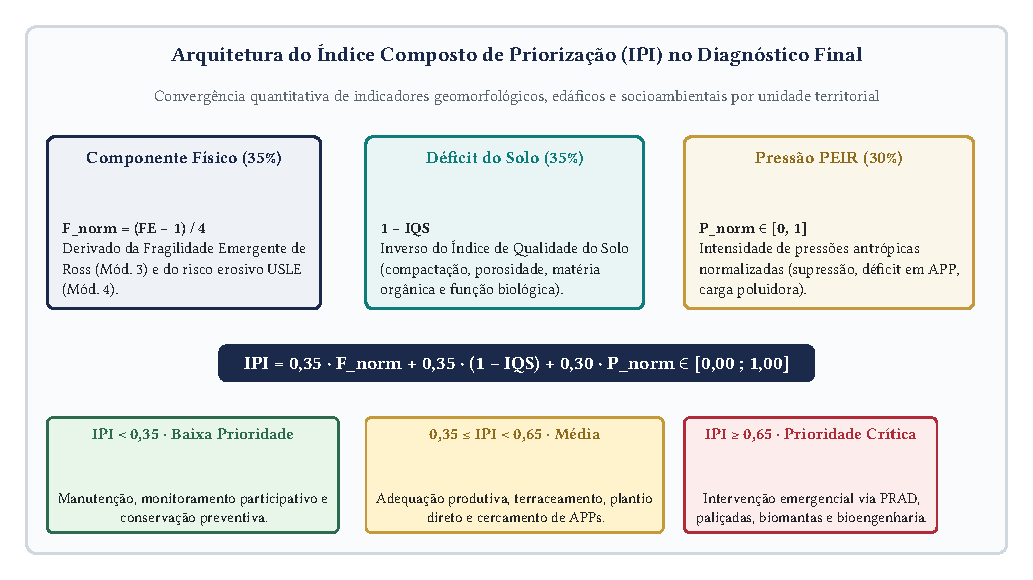
\includegraphics[width=0.94\textwidth]{figures/fig_cap15_matriz_ipi_priorizacao.pdf}
  \caption{Arquitetura conceitual do Índice Composto de Priorização de Intervenção ($IPI$), articulando o componente físico ($F_{\text{norm}}$), o déficit do solo ($1 - IQS$) e a pressão PEIR ($P_{\text{norm}}$) em faixas de decisão.}
  \label{fig:matriz_ipi_priorizacao}
\end{figure}

As quatro faixas operacionais empregadas na classificação detalhada dos setores da microbacia constam da Tabela~\ref{tab:faixas_ipi}, orientando desde o monitoramento preventivo em remanescentes conservados até obras integradas de drenagem e bioengenharia nos setores críticos.

\begin{table}[H]
\centering
\caption{Faixas operacionais de priorização do $IPI$ e diretrizes de gestão correspondentes.}
\label{tab:faixas_ipi}
\renewcommand{\arraystretch}{1.15}
\small
\begin{tabularx}{\textwidth}{@{}c l >{\raggedright\arraybackslash}X@{}}
  \toprule
  \rowcolor{uefsNavy}
  \textcolor{white}{\bfseries Intervalo de $IPI$} & \textcolor{white}{\bfseries Classe de Prioridade} & \textcolor{white}{\bfseries Diretriz de Gestão e Intervenção} \\
  \midrule
  $0{,}00 \le IPI < 0{,}35$ & \textbf{Baixa} & Conservação preventiva e monitoramento periódico. \\
  \rowcolor{bgGray}
  $0{,}35 \le IPI < 0{,}60$ & \textbf{Média} & Práticas conservacionistas ($C$ e $P$) e manejo sustentável. \\
  $0{,}60 \le IPI < 0{,}80$ & \textbf{Alta} & Bioengenharia leve (biomantas, estacas vivas) e recomposição de APP. \\
  \rowcolor{bgGray}
  $0{,}80 \le IPI \le 1{,}00$ & \textbf{Crítica} & Intervenção imediata integrada (PRAD, paliçadas, drenagem e isolamento). \\
  \bottomrule
\end{tabularx}
\end{table}

Na organização prática do relatório, os indicadores levantados em SIG, campo e laboratório articulam-se em uma matriz integrada que vincula diretamente cada métrica mensurada à respectiva resposta corretiva de PRAD ou bioengenharia (Tabela~\ref{tab:matriz_integrada_ipi}). O Exemplo 15.2 demonstra o cálculo passo a passo do $IPI$ para três setores contrastantes de uma microbacia.

\begin{table}[H]
\centering
\caption{Estrutura de referência da Matriz Integrada de Indicadores para o Trabalho Prático Final.}
\label{tab:matriz_integrada_ipi}
\renewcommand{\arraystretch}{1.18}
\small
\begin{tabularx}{\textwidth}{@{}p{2.0cm} p{2.8cm} p{2.8cm} p{2.6cm} >{\raggedright\arraybackslash}X@{}}
  \toprule
  \rowcolor{uefsNavy}
  \textcolor{white}{\bfseries Dimensão} & \textcolor{white}{\bfseries Indicador Medido} & \textcolor{white}{\bfseries Fonte / Método} & \textcolor{white}{\bfseries Valor / Classe} & \textcolor{white}{\bfseries Papel na Resposta (PRAD)} \\
  \midrule
  \textbf{PEIR (P)} & Déficit de APP marginal & SICAR + MapBiomas & $35\%$ suprimido & Recomposição legal obrigatória (Lei 12.651/12). \\
  \rowcolor{bgGray}
  \textbf{PEIR (E) / Solo} & Densidade do solo ($D_s$) e $IQS$ & Anel volumétrico / MDS & $IQS = 0{,}42$ (Baixo) & Descompactação e aporte de matéria orgânica. \\
  \textbf{Ross (FE)} & Fragilidade Emergente & Cruzamento decliv., solo e uso & $FE = 4$ (Forte) & Restrição de uso e cobertura permanente. \\
  \rowcolor{bgGray}
  \textbf{PEIR (I)} & Focos erosivos lineares & Campo / Imagem alta res. & $4\text{ ravinas/km}^2$ & Paliçadas permeáveis e dissipadores de energia. \\
  \bottomrule
\end{tabularx}
\end{table}

\begin{boxExemplo}{15.2 (Intermediário)}{Montagem da Matriz Integrada e Cálculo do $IPI$ por Setor}
\passoEnunciado{Ao organizar a Matriz de Indicadores do Trabalho Final, uma equipe dividiu uma microbacia em três setores homogêneos e levantou, por meio de QGIS, campo e análise de solo, os valores de Fragilidade Emergente ($FE$), Índice de Qualidade do Solo ($IQS$) e Pressão/Impacto PEIR normalizado ($P_{\text{norm}}$).}
\passoDados{\textbf{Setor A (Cabeceira com voçoroca):} $FE = 5$, $IQS = 0{,}36$, $P_{\text{norm}} = 0{,}90$. \textbf{Setor B (Meia encosta com pastagem):} $FE = 3$, $IQS = 0{,}60$, $P_{\text{norm}} = 0{,}50$. \textbf{Setor C (Remanescente de Caatinga/APP):} $FE = 2$, $IQS = 0{,}88$, $P_{\text{norm}} = 0{,}10$. Pesos adotados iguais a $w_F = 0{,}35$, $w_S = 0{,}35$ e $w_P = 0{,}30$.}
\passoPedido{Calcular $F_{\text{norm}}$, $(1 - IQS)$ e o Índice Composto de Priorização ($IPI$) para cada setor, classificando a prioridade de intervenção.}
\passoMetodo{Normalização de $FE$ por $F_{\text{norm}} = (FE - 1)/4$ e aplicação da soma ponderada $IPI = 0{,}35\,F_{\text{norm}} + 0{,}35\,(1 - IQS) + 0{,}30\,P_{\text{norm}}$.}
\passoContas{%
\textbf{Setor A:} $F_{\text{norm}} = (5 - 1)/4 = 1{,}00$ e $(1 - IQS) = 1 - 0{,}36 = 0{,}64$:
\begin{align*}
IPI_A &= 0{,}35(1{,}00) + 0{,}35(0{,}64) + 0{,}30(0{,}90) \\
      &= 0{,}350 + 0{,}224 + 0{,}270 = \mathbf{0{,}844}\quad(\text{Prioridade Crítica})
\end{align*}
\textbf{Setor B:} $F_{\text{norm}} = (3 - 1)/4 = 0{,}50$ e $(1 - IQS) = 1 - 0{,}60 = 0{,}40$:
\begin{align*}
IPI_B &= 0{,}35(0{,}50) + 0{,}35(0{,}40) + 0{,}30(0{,}50) \\
      &= 0{,}175 + 0{,}140 + 0{,}150 = \mathbf{0{,}465}\quad(\text{Prioridade Média})
\end{align*}
\textbf{Setor C:} $F_{\text{norm}} = (2 - 1)/4 = 0{,}25$ e $(1 - IQS) = 1 - 0{,}88 = 0{,}12$:
\begin{align*}
IPI_C &= 0{,}35(0{,}25) + 0{,}35(0{,}12) + 0{,}30(0{,}10) \\
      &= 0{,}0875 + 0{,}0420 + 0{,}0300 = \mathbf{0{,}1595}\approx \mathbf{0{,}160}\quad(\text{Prioridade Baixa})
\end{align*}}
\passoResposta{$IPI_A = \mathbf{0{,}844}$ (Crítica, PRAD e bioengenharia imediatos); $IPI_B = \mathbf{0{,}465}$ (Média, manejo conservacionista); $IPI_C = \mathbf{0{,}160}$ (Baixa, manutenção e monitoramento).}
\passoVerificacao{Todos os valores permanecem dentro do intervalo teórico $[0,\,1]$, e a ordenação ($A > B > C$) reflete fielmente o gradiente de degradação observado.}
\end{boxExemplo}

\section{Etapa 6: Produtos Técnicos Obrigatórios e Proposta de Intervenção}

O trabalho entregue deve conter três produtos técnicos articulados entre si. O primeiro produto consiste no \textbf{conjunto de mapas temáticos}, composto por no mínimo três cartas principais, sendo elas o Mapa de Localização e Delimitação do Recorte Espacial, o Mapa de Uso e Cobertura da Terra e APPs, e o Mapa de Fragilidade Ambiental e Pontos de Degradação; todos os layouts devem apresentar os \textbf{seis elementos cartográficos obrigatórios} (título informativo, orientação com seta Norte, escala gráfica e numérica, grade de coordenadas com indicação do datum \textbf{SIRGAS 2000}, legenda legível e quadro de fontes e autoria).

O segundo produto corresponde ao \textbf{relatório técnico interpretativo}, redigido de forma estruturada com introdução e objetivos, localização e métodos, resultados integrados (apoiados em tabelas, gráficos e matriz de indicadores) e discussão crítica fundamentada na bibliografia da disciplina. Articulando-se diretamente a esse diagnóstico, o terceiro produto reúne a \textbf{proposta preliminar de conservação, bioengenharia ou PRAD}, vinculando cada medida aos indicadores críticos diagnosticados (Vital et al., 2020) mediante especificação das técnicas selecionadas (paliçadas, biomantas, plantio em contorno, isolamento de APP e espécies nativas), cronograma físico simplificado e metas mensuráveis de monitoramento pós-implantação, como taxa de sobrevivência $\ge 80\%$ e redução do recuo de borda erosiva.

Toda recomendação técnica deve indicar qual processo físico será alterado e por qual mecanismo, respeitando o percurso da água entre fontes a montante, caminhos de escoamento e áreas receptoras a jusante. Além disso, cada conclusão precisa manter vínculo verificável com os dados coletados, explicitando o alcance descritivo de evidências fotográficas frente a medições instrumentais (como densidade do solo, infiltração e perfis transversais), justificando os pesos adotados na matriz de prioridade e registrando dados ausentes e eventuais incertezas sobre a decisão. Os Exemplos 15.3 e 15.4 ilustram, respectivamente, a quantificação do passivo em APP para o dimensionamento de mudas e a seleção de intervenções por custo-efetividade ($CE$).

\begin{boxExemplo}{15.3 (Intermediário)}{Quantificação de Passivo em APP Marginal e Demanda de Mudas}
\passoEnunciado{Na sobreposição entre a hidrografia vetorial, o SICAR e o MapBiomas, uma equipe diagnosticou um trecho de $2.000\text{ m}$ de curso d'água com $12\text{ m}$ de largura regular, no qual a mata ciliar foi parcialmente substituída por pastagem degradada.}
\passoDados{Comprimento do trecho $L = 2.000\text{ m}$; largura do rio de $12\text{ m}$ (pela Lei nº 12.651/2012, cursos d'água entre $10\text{ m}$ e $50\text{ m}$ exigem APP mínima de $50\text{ m}$ em cada margem); percentual degradado diagnosticado nas duas margens de $35\%$; espaçamento adotado no PRAD de $2{,}5\text{ m} \times 2{,}0\text{ m}$ ($5{,}0\text{ m}^2$ por muda, equivalente a $2.000\text{ mudas}\cdot\text{ha}^{-1}$), prevendo $10\%$ adicionais para replantio.}
\passoPedido{Calcular a área total de APP legal no trecho, o passivo ambiental em hectares a ser recomposto e o número total de mudas nativas necessário.}
\passoMetodo{Cálculo geométrico da área retangular equivalente das duas faixas marginais, aplicação do percentual de déficit e multiplicação pela densidade de plantio ajustada para replantio.}
\passoContas{%
\textbf{Etapa 1, Área total de APP legal (duas margens) e passivo a recompor ($35\%$):}
\[
A_{\text{APP}} = 2 \times 50\text{ m} \times 2.000\text{ m} = 200.000\text{ m}^2 = \mathbf{20{,}0\text{ ha}} \qquad A_{\text{passivo}} = 0{,}35 \times 20{,}0 = \mathbf{7{,}0\text{ ha}}
\]
\textbf{Etapa 2, Quantidade inicial de mudas e total com $10\%$ de replantio:}
\[
N_{\text{inicial}} = 7{,}0 \times 2.000 = 14.000\text{ mudas} \qquad\qquad N_{\text{total}} = 14.000 \times 1{,}10 = \mathbf{15.400\text{ mudas}}
\]}
\passoResposta{APP total $= \mathbf{20{,}0\text{ ha}}$; passivo a recompor $= \mathbf{7{,}0\text{ ha}}$; demanda total do viveiro $= \mathbf{15.400\text{ mudas nativas}}$.}
\passoVerificacao{Para $7{,}0\text{ ha}$, o número inicial de $14.000$ mudas equivale exatamente a $1$ muda a cada $5\text{ m}^2$ ($70.000 / 5 = 14.000$), e o acréscimo de $10\%$ ($1.400$ mudas) garante a reposição de eventuais perdas no primeiro ciclo seco.}
\end{boxExemplo}

Quando múltiplas alternativas técnicas atendem ao mesmo diagnóstico, a comparação financeira pela retenção anual de sedimentos orienta a alocação eficiente de recursos no relatório final (Exemplo 15.4).

\begin{boxExemplo}{15.4 (Avançado)}{Seleção de Alternativa de Intervenção por Custo-Efetividade ($CE$)}
\passoEnunciado{Para conter o aporte de sedimentos em uma ravina crítica ($IPI = 0{,}84$) identificada no Trabalho Final, a equipe comparou duas propostas preliminares de intervenção, confrontando o Pacote 1 (paliçadas permeáveis de bambu, biomanta e revegetação com espécies nativas) com o Pacote 2 (enrocamento com gabiões de pedra e canaleta rígida de concreto).}
\passoDados{\textbf{Pacote 1 (Bioengenharia e PRAD):} custo estimado $= \reais{18.000,00}$; retenção anual estimada $= 180\text{ t}\cdot\text{ano}^{-1}$ de sedimentos. \textbf{Pacote 2 (Obra Rígida Convencional):} custo estimado $= \reais{45.000,00}$; retenção anual estimada $= 225\text{ t}\cdot\text{ano}^{-1}$ de sedimentos.}
\passoPedido{Calcular o Custo-Efetividade ($CE$) de cada pacote em $\text{t}\cdot\text{ano}^{-1}$ retidas por $\reais{1.000,00}$ investidos e justificar a recomendação técnica no relatório.}
\passoMetodo{Divisão da massa anual de sedimentos retida pelo custo total expresso em milhares de reais.}
\passoContas{%
\textbf{Etapa 1, Pacote 1 (Bioengenharia) e Pacote 2 (Obra Rígida):}
\begin{align*}
CE_1 &= \frac{180\text{ t}\cdot\text{ano}^{-1}}{18{,}0\text{ mil reais}} = \mathbf{10{,}0\text{ t}\cdot\text{ano}^{-1}\text{ por }\reais{1.000,00}} \\
CE_2 &= \frac{225\text{ t}\cdot\text{ano}^{-1}}{45{,}0\text{ mil reais}} = \mathbf{5{,}0\text{ t}\cdot\text{ano}^{-1}\text{ por }\reais{1.000,00}}
\end{align*}}
\passoResposta{$CE_1 = \mathbf{10{,}0\text{ t}\cdot\text{ano}^{-1}\text{ por }\reais{1.000,00}}$ e $CE_2 = \mathbf{5{,}0\text{ t}\cdot\text{ano}^{-1}\text{ por }\reais{1.000,00}}$. O Pacote 1 (Bioengenharia e PRAD) é \textbf{duas vezes mais custo-efetivo}, além de restabelecer funções ecológicas e infiltração.}
\passoVerificacao{O Pacote 2 retém $25\%$ a mais de sedimentos ($225$ contra $180\text{ t}\cdot\text{ano}^{-1}$), porém custa $2{,}5$ vezes mais ($\reais{45.000}$ contra $\reais{18.000}$), indicando vantagem técnica e econômica da bioengenharia em ravinas de pequeno e médio porte.}
\end{boxExemplo}

Esse encadeamento entre diagnóstico espacial, matriz quantitativa e prescrição executiva previne propostas genéricas desconectadas das evidências de campo.

\begin{boxErro}[Erro 3: Apresentar Diagnóstico Desconectado da Proposta de Intervenção]
\textbf{Equívoco frequente:} Descrever no relatório uma voçoroca ativa com \textit{piping} e compactação severa, mas propor na conclusão apenas ``conscientização ambiental'' ou ``plantio aleatório de mudas'' sem controle de escoamento.\par
\textbf{Correção técnica:} Cada medida da proposta de PRAD ou bioengenharia deve responder diretamente a um indicador crítico da Matriz de Indicadores ($IPI$), articulando controle hidráulico a montante, estabilização mecânica (paliçadas ou biomantas) e recomposição vegetal adaptada ao bioma.
\end{boxErro}

\section{Etapa 7: Checklist de Entrega e Rubrica Oficial de Avaliação (5,0 Pontos)}

Na Semana 16, o trabalho é entregue e socializado em apresentação oral breve. Utilize a rubrica oficial apresentada na Tabela~\ref{tab:rubrica_tpf} para auditar seu projeto antes da submissão final.

\begin{table}[H]
\centering
\caption{Rubrica oficial de avaliação do Trabalho Prático Final da disciplina CHF662 (Semana 16, $5{,}0$ pontos).}
\label{tab:rubrica_tpf}
\renewcommand{\arraystretch}{1.20}
\small
\begin{tabularx}{\textwidth}{@{}p{3.6cm} c >{\raggedright\arraybackslash}X@{}}
  \toprule
  \rowcolor{uefsNavy}
  \textcolor{white}{\bfseries Critério Avaliativo} & \textcolor{white}{\bfseries Peso (pts)} & \textcolor{white}{\bfseries Descritor de Desempenho Pleno (100\%)} \\
  \midrule
  \textbf{1. Delimitação e Bases Cartográficas} & $1{,}0$ & Recorte espacial justificado; bases abertas validadas (IBGE, TOPODATA, MapBiomas, SICAR); todos os mapas em SIRGAS 2000 com os 6 elementos obrigatórios. \\
  \rowcolor{bgGray}
  \textbf{2. Caracterização Integrada e Degradação} & $1{,}0$ & Articulação físico-biótica e socioespacial sem fragmentação; processos erosivos e passivos em APP corretamente classificados e georreferenciados. \\
  \textbf{3. Matriz de Indicadores ($IPI$ / PEIR / Solo / Ross)} & $1{,}0$ & Matriz completa e coerente, sem inversão de categorias PEIR; cálculos de $IQS$, Ross e $IPI$ auditáveis e interpretados. \\
  \rowcolor{bgGray}
  \textbf{4. Produtos Técnicos e Proposta de PRAD/Bioengenharia} & $1{,}2$ & Proposta tecnicamente compatível com os processos diagnosticados (Vital et al., 2020), respeitando a Lei nº 12.651/2012 e com metas de monitoramento. \\
  \textbf{5. Redação Técnica e Socialização (Semana 16)} & $0{,}8$ & Clareza, norma culta, citações padronizadas (ABNT) e defesa oral objetiva, respeitando o tempo e respondendo com domínio conceitual. \\
  \midrule
  \textbf{TOTAL GERAL} & $\mathbf{5{,}0}$ & \textbf{Correspondente a $50\%$ da média semestral de CHF662.} \\
  \bottomrule
\end{tabularx}
\end{table}

\etapa{4}{Síntese Aplicada: Auditoria Pré-Entrega pela Rubrica Oficial}

Antes de submeter a versão definitiva do relatório e dos mapas na Semana 16, recomenda-se executar uma auditoria interna com base nos cinco critérios da rubrica, identificando onde ajustes objetivos geram o maior ganho de qualidade técnica (Exemplo 15.5).

\begin{boxExemplo}{15.5 (Aplicado)}{Auditoria Pré-Entrega pela Rubrica Oficial CHF662 ($5{,}0$ Pontos)}
\passoEnunciado{Uma semana antes da socialização da Semana 16, um grupo realizou uma simulação de autoavaliação de seu rascunho de Trabalho Prático Final utilizando a Rubrica Oficial de $5{,}0$ pontos da disciplina CHF662.}
\passoDados{Notas parciais diagnosticadas na pré-auditoria: Critério 1 (Delimitação e bases, máx. $1{,}0$) igual a $0{,}70$ por ausência de datum SIRGAS 2000 e escala gráfica em um dos mapas; Critério 2 (Caracterização e degradação, máx. $1{,}0$) igual a $0{,}90$; Critério 3 (Matriz de Indicadores, máx. $1{,}0$) igual a $1{,}00$; Critério 4 (Produtos técnicos e PRAD, máx. $1{,}2$) igual a $0{,}85$ por ausência de metas mensuráveis de monitoramento no PRAD; e Critério 5 (Redação e socialização, máx. $0{,}8$) igual a $0{,}75$.}
\passoPedido{Calcular a pontuação atual do rascunho, o percentual atingido sobre os $5{,}0$ pontos e identificar quais duas correções rápidas recuperam o maior ganho de nota antes da entrega.}
\passoMetodo{Soma ponderada direta das notas obtidas nos cinco critérios e cálculo do déficit por critério.}
\passoContas{%
\textbf{Etapa 1, Pontuação atual do rascunho e percentual sobre $5{,}0$ pontos:}
\[
N_{\text{atual}} = 0{,}70 + 0{,}90 + 1{,}00 + 0{,}85 + 0{,}75 = \mathbf{4{,}20\text{ pontos}} \qquad\qquad \frac{4{,}20}{5{,}00} \times 100\% = \mathbf{84{,}0\%}
\]
\textbf{Etapa 2, Maiores déficits identificados na rubrica:} Critério 4 ($1{,}20 - 0{,}85 = 0{,}35\text{ pt}$) e Critério 1 ($1{,}00 - 0{,}70 = 0{,}30\text{ pt}$).}
\passoResposta{Pontuação atual $= \mathbf{4{,}20\text{ pts}}$ ($84{,}0\%$). Inserir metas mensuráveis de monitoramento no PRAD ($+0{,}35\text{ pt}$) e completar o datum SIRGAS 2000 e a escala gráfica no mapa ($+0{,}30\text{ pt}$) eleva o trabalho para $4{,}85\text{ pts}$ ($97{,}0\%$).}
\passoVerificacao{A soma das perdas totais ($0{,}30 + 0{,}10 + 0{,}00 + 0{,}35 + 0{,}05 = 0{,}80\text{ pt}$) fecha exatamente com $5{,}00 - 4{,}20 = 0{,}80\text{ pt}$.}
\end{boxExemplo}

\etapa{5}{Armadilha Conceitual e Materiais Audiovisuais de Apoio}

Mesmo com mapas bem elaborados e cálculos corretos, a inversão causal entre os compartimentos da Matriz de Indicadores invalida a coerência entre diagnóstico e proposta de recuperação.

\begin{boxErro}[Erro 4: Confundir Indicadores de Pressão, Estado, Impacto e Resposta na Matriz]
\textbf{Equívoco frequente:} Listar a execução do PRAD como ``Impacto'' ou classificar a declividade natural do relevo como ``Pressão antrópica''.\par
\textbf{Correção técnica:} Lembre a cadeia causal do modelo PEIR. O compartimento \textbf{P} reúne o vetor ou atividade humana modificadora; \textbf{E} retrata a condição atual do meio; \textbf{I} traduz o efeito físico, ecológico ou social mensurável; e \textbf{R} expressa a ação corretiva, legal ou de manejo proposta pelo poder público ou empreendedor.
\end{boxErro}

\begin{sloppypar}
Para revisar a articulação entre legislação ambiental, Código Florestal e instrumentos de gestão aplicados ao Trabalho Prático Final, assista às videoaulas selecionadas na página da disciplina, iniciando por \textit{Gestão Ambiental - Legislação e Certificação Ambiental} (\url{https://www.youtube.com/watch?v=L-WEcC2IlbA}), prosseguindo com \textit{Direito Ambiental: Código Florestal} (\url{https://www.youtube.com/watch?v=ApidLjWC4Dc}) e concluindo com \textit{Legislação Ambiental Brasileira} (\url{https://www.youtube.com/watch?v=gC4uHPJDiVA}).
\end{sloppypar}

\etapa{6}{Exercícios de Fixação}

\subsection*{Nível Básico (Conceitos, Bases Abertas e Fluxo do Trabalho Final)}

\begin{enumerate}[leftmargin=1.8em, itemsep=6pt]
  \item Explique por que a \textbf{microbacia hidrográfica} é considerada a unidade espacial preferencial para o Trabalho Prático Final da disciplina CHF662, citando ao menos duas vantagens analíticas em relação a recortes puramente administrativos.
  \espacoResolucao[1.8cm]

  \item Relacione as cinco plataformas abertas (\textbf{IBGE}, \textbf{TOPODATA/SRTM}, \textbf{MapBiomas}, \textbf{SICAR/CAR} e \textbf{INEMA/SEI-BA}) ao tipo específico de dado que cada uma fornece para o diagnóstico ambiental.
  \espacoResolucao[1.8cm]

  \item Liste os \textbf{seis elementos cartográficos obrigatórios} que devem constar em todos os mapas temáticos do Trabalho Prático Final e explique qual datum oficial deve ser adotado no Brasil.
  \espacoResolucao[1.8cm]

  \item Diferencie \textbf{diagnóstico descritivo fragmentado} de \textbf{caracterização integrada físico-biótica e socioespacial}, exemplificando com uma relação causal entre uso da terra e processo erosivo.
  \espacoResolucao[1.8cm]

  \item Descreva os três componentes integrados na fórmula do \textbf{Índice Composto de Priorização de Intervenção ($IPI$)} e explique por que um setor com $IPI \ge 0{,}80$ demanda ação imediata.
  \espacoResolucao[1.8cm]
\end{enumerate}

\subsection*{Nível Intermediário (Escala, Matriz $IPI$, Passivo de APP e Rubrica)}

\begin{enumerate}[leftmargin=1.8em, itemsep=6pt, resume]
  \item Considerando o critério cartográfico de área mínima legível no papel de $4\text{ mm}^2$, calcule a área mínima mapeável no terreno ($A_{\min}$, em $\text{m}^2$ e em $\text{ha}$) para as escalas $1:15.000$ e $1:50.000$.
  \espacoResolucao[2.2cm]

  \item Uma vertente analisada no Trabalho Final apresentou Fragilidade Emergente de Ross $FE = 4$, Índice de Qualidade do Solo $IQS = 0{,}48$ e Pressão/Impacto normalizado $P_{\text{norm}} = 0{,}80$. Adotando os pesos padrão ($w_F = 0{,}35$, $w_S = 0{,}35$, $w_P = 0{,}30$), calcule o $IPI$ e classifique a prioridade de intervenção.
  \espacoResolucao[2.2cm]

  \item Um córrego com $8\text{ m}$ de largura atravessa $1.500\text{ m}$ de uma microbacia (APP legal de $30\text{ m}$ em cada margem). Verificou-se que $40\%$ da APP da margem esquerda e $20\%$ da APP da margem direita estão degradadas. Calcule a área total a recompor (em $\text{ha}$) e o número de mudas necessário no espaçamento de $2{,}5\text{ m} \times 2{,}0\text{ m}$ ($2.000\text{ mudas}\cdot\text{ha}^{-1}$), sem considerar replantio adicional.
  \espacoResolucao[2.2cm]

  \item Para estabilizar uma margem fluvial, o Pacote A (estacas vivas + biomanta) custa $\reais{12.000,00}$ e retém $144\text{ t}\cdot\text{ano}^{-1}$ de sedimentos, enquanto o Pacote B (muro de concreto) custa $\reais{25.000,00}$ e retém $200\text{ t}\cdot\text{ano}^{-1}$. Calcule o Custo-Efetividade ($CE$) de ambos em $\text{t}\cdot\text{ano}^{-1}$ por $\reais{1.000,00}$ e indique o mais vantajoso.
  \espacoResolucao[2.2cm]

  \item Na avaliação da Semana 16, um grupo obteve as seguintes notas nos cinco critérios da rubrica oficial: $0{,}90$ (Critério 1), $0{,}80$ (Critério 2), $0{,}80$ (Critério 3), $1{,}00$ (Critério 4) e $0{,}70$ (Critério 5). Calcule a nota final do Trabalho Prático (de $0$ a $5{,}0$) e o percentual de aproveitamento.
  \espacoResolucao[2.2cm]
\end{enumerate}

\subsection*{Nível Aplicado (Questões Objetivas A--E)}

\begin{enumerate}[leftmargin=1.8em, itemsep=6pt, resume]
  \item Na elaboração de mapas temáticos em QGIS para o Diagnóstico Ambiental Aplicado no Estado da Bahia, o procedimento correto para calcular áreas de uso da terra e extensão de APPs em hectares e metros é:
  \begin{alternativas}
    \item Manter as camadas em graus decimais sem projeção plana e multiplicar graus por $100$.
    \item Reprojetar as camadas vetoriais e matriciais para o sistema de coordenadas planas métricas \textbf{SIRGAS 2000 / UTM} correspondente ao fuso local.
    \item Utilizar apenas o sistema norte-americano NAD27 em milhas quadradas.
    \item Desenhar o polígono manualmente sobre uma captura de tela sem escala.
    \item Omitir a grade de coordenadas e o datum para simplificar o layout.
  \end{alternativas}

  \item Para mapear o relevo, extrair curvas de nível, delimitar automaticamente uma microbacia e calcular o mapa de declividades da matriz de Ross em um diagnóstico com dados abertos, a fonte prioritária é:
  \begin{alternativas}
    \item Apenas o censo demográfico decenal do IBGE.
    \item Modelos Digitais de Elevação gratuitos como \textbf{SRTM} ou \textbf{TOPODATA/INPE}.
    \item Exclusivamente entrevistas orais sem base altimétrica.
    \item Somente boletins de balneabilidade de praias oceânicas.
    \item Plantas arquitetônicas internas de edificações urbanas.
  \end{alternativas}

  \item Na etapa de verificação de passivos florestais em propriedades rurais dentro da microbacia de estudo, o cruzamento de dados abertos mais indicado é:
  \begin{alternativas}
    \item Rede viária federal cruzada com dados de radiação solar.
    \item Perímetros do \textbf{SICAR/CAR} e hidrografia oficial cruzados com as séries de uso e cobertura da terra do \textbf{MapBiomas}.
    \item Apenas mapas geológicos na escala $1:5.000.000$.
    \item Exclusivamente dados de arrecadação tributária municipal.
    \item Cartas náuticas oceânicas cruzadas com limites de bairros metropolitanos.
  \end{alternativas}

  \item Um setor de uma microbacia recebeu Fragilidade Emergente $FE = 5$, Índice de Qualidade do Solo $IQS = 0{,}40$ e Pressão/Impacto normalizado $P_{\text{norm}} = 0{,}70$. Usando os pesos padrão ($w_F = 0{,}35$, $w_S = 0{,}35$, $w_P = 0{,}30$), o valor de $IPI$ e sua classe de prioridade são:
  \begin{alternativas}
    \item $0{,}560$ (Prioridade Média).
    \item $0{,}665$ (Prioridade Alta).
    \item $0{,}770$ (Prioridade Alta).
    \item $0{,}840$ (Prioridade Crítica).
    \item $0{,}910$ (Prioridade Crítica).
  \end{alternativas}

  \item Sobre a estrutura dos produtos técnicos e a rubrica de avaliação da Semana 16 (CHF662), assinale a alternativa \textbf{INCORRETA}:
  \begin{alternativas}
    \item O Trabalho Prático Final corresponde a $5{,}0$ pontos ($50\%$ da média semestral) e inclui entrega técnica e socialização oral.
    \item A Matriz de Indicadores deve articular o modelo PEIR, a qualidade do solo e a fragilidade ambiental de Ross.
    \item A proposta preliminar de intervenção (PRAD/bioengenharia) deve conter metas mensuráveis de monitoramento pós-implantação.
    \item Os mapas temáticos devem trazer título, Norte, escala, coordenadas/datum, legenda e fonte.
    \item A rubrica atribui $100\%$ da nota apenas à quantidade de páginas do relatório, dispensando coerência entre diagnóstico, legislação e proposta técnica.
  \end{alternativas}
\end{enumerate}

\etapa{7}{Questões no Estilo ENADE e Concursos Ambientais}

\begin{boxDica}[Da Universidade para a Prática Profissional]
Em editais de Analista Ambiental (IBAMA, ICMBio, INEMA) e no ENADE de Geografia, exige-se que o candidato saiba encadear base cartográfica, indicador mensurável, enquadramento legal e técnica de recuperação. Esse fluxo completo fundamenta tanto o Trabalho Prático Final quanto a atuação profissional em consultoria e gestão pública.
\end{boxDica}

\begin{enumerate}[leftmargin=1.8em, itemsep=7pt]
  \item \textbf{[Questão Autoral, Estilo ENADE / Geografia]} Ao coordenar um diagnóstico ambiental aplicado em uma microbacia rural do Semiárido baiano (IBGE, 2018; Cavalcanti, 2006), um geógrafo constatou que os dados altimétricos tinham resolução de $30\text{ m}$ (TOPODATA), o uso da terra provinha do MapBiomas ($30\text{ m}$) e as feições erosivas críticas (ravinas de $2\text{ m}$ de largura) foram georreferenciadas em campo com GPS e fotografadas com escala métrica. A postura metodológica mais rigorosa ao integrar essas fontes no relatório final é:
  \begin{alternativas}
    \item Descartar os dados de campo para manter apenas pixels de $30\text{ m}$, ainda que ocultem ravinas estreitas.
    \item Apresentar os mapas de bacia e uso na escala compatível com as bases regionais ($1:25.000$ a $1:50.000$), explicitando suas limitações de resolução, e representar as ravinas por pontos/linhas georreferenciados em escala de detalhe no diagnóstico local.
    \item Redimensionar artificialmente o raster de $30\text{ m}$ para $0{,}10\text{ m}$ e afirmar no relatório que o satélite possui precisão centimétrica.
    \item Omitir a escala gráfica e a fonte dos dados para evitar questionamentos metodológicos.
    \item Misturar camadas em SIRGAS 2000 geográfico e UTM sem reprojeção, aceitando distorções de área.
  \end{alternativas}

  \item \textbf{[Questão Autoral, Estilo Concurso Analista Ambiental / PRAD]} Em um diagnóstico integrado para subsidiar um PRAD (Vital et al., 2020), identificaram-se três problemas simultâneos em uma área degradada: (i) solo superficial compactado ($D_s = 1{,}66\text{ g}\cdot\text{cm}^{-3}$); (ii) escoamento pluvial concentrado descendo de uma estrada vicinal sem drenagem; e (iii) ausência de vegetação em $45\text{ m}$ de APP marginal. Qual sequência de ações respeita a lógica física e legal da recuperação ambiental?
  \begin{alternativas}
    \item Plantar árvores de grande porte dentro da estrada vicinal sem desviar a enxurrada e deixar o solo compactado.
    \item Aplicar apenas herbicida na margem do rio e aguardar a regeneração espontânea sem controle hidráulico.
    \item Implantar primeiro o disciplinamento e desvio das águas pluviais da estrada (dissipadores e terraços), realizar escarificação e incorporação de matéria orgânica no solo compactado, instalar contenções leves (paliçadas e biomantas) nos pontos críticos e executar o plantio de espécies nativas na APP com monitoramento periódico.
    \item Substituir toda a APP por pavimentação asfáltica para impedir a infiltração da água da chuva.
    \item Solicitar dispensa automática do PRAD alegando que estradas vicinais não produzem sedimentos.
  \end{alternativas}

  \item \textbf{[Questão Autoral, Estilo Concurso Geógrafo / Gestão Territorial]} Um órgão ambiental estadual recebeu dois relatórios de diagnóstico para análise. O Relatório X apresentou apenas descrições gerais do município, sem delimitação de bacia, sem indicadores quantitativos e sem proposta de monitoramento. O Relatório Y delimitou a microbacia em SIRGAS 2000/UTM, integrou matriz PEIR, IQS e Fragilidade de Ross, quantificou o déficit de APP pelo Código Florestal e propôs técnicas de bioengenharia com metas semestrais auditáveis. Sob a ótica da Análise Ambiental (Sánchez, 2013; IBGE, 2018), o Relatório Y distingue-se por assegurar:
  \begin{alternativas}
    \item Subjetividade estética sem vínculo com parâmetros físicos ou legais.
    \item Rastreabilidade metodológica, mensurabilidade de indicadores, conformidade jurídica e viabilidade de fiscalização das respostas propostas.
    \item Substituição completa do trabalho de campo por opiniões informais.
    \item Isenção de responsabilidade técnica do autor pela ausência de números.
    \item Impossibilidade de comparação temporal futura em razão do uso de indicadores numéricos.
  \end{alternativas}
\end{enumerate}

\clearpage
\etapa{8}{Gabarito Comentado do Capítulo 15}

\begin{boxGabarito}[Resoluções Completas: Exercícios de Fixação (1 a 15)]
\begin{enumerate}[leftmargin=1.6em, itemsep=4pt]
  \item A microbacia possui limites físicos naturais definidos pelos divisores topográficos e integra em um único sistema os fluxos de água, sedimentos, nutrientes e usos da terra. Duas vantagens: (a) permite fechar balanços hídricos e hidrossedimentológicos (erosão na vertente $\rightarrow$ assoreamento no exutório); e (b) evidencia interdependências entre propriedades a montante e a jusante que recortes municipais ou de lotes isolados ocultam.
  \item \textbf{IBGE:} limites territoriais, malha censitária, hidrografia e pedologia; \textbf{TOPODATA/SRTM:} MDE ($30\text{ m}$), declividade, curvas de nível e delimitação de bacias; \textbf{MapBiomas:} séries históricas anuais de uso e cobertura da terra; \textbf{SICAR/CAR:} limites de imóveis rurais, APPs e Reserva Legal declaradas; \textbf{INEMA/SEI-BA:} outorgas, licenciamento, dados climáticos e informações socioeconômicas estaduais.
  \item Os seis elementos obrigatórios são: (1) título informativo; (2) orientação (seta Norte); (3) escala gráfica e numérica; (4) grade de coordenadas com indicação do datum; (5) legenda; e (6) quadro de fontes e autoria. O datum oficial obrigatório no Brasil é o \textbf{SIRGAS 2000}.
  \item Um diagnóstico descritivo fragmentado lista clima, solo, vegetação e população em seções isoladas sem explicar suas conexões. Já a caracterização integrada indica relações causais, como explicar de que modo a substituição da Caatinga por pastagem extensiva (dinâmica socioespacial) reduz a cobertura vegetal, eleva a compactação superficial e acelera o ravinamento em vertentes de Neossolo (meio físico-biótico).
  \item O $IPI$ combina: (1) Fragilidade Emergente de Ross normalizada ($F_{\text{norm}}$); (2) Déficit de Qualidade do Solo ($1 - IQS$); e (3) Pressão/Impacto antrópico da matriz PEIR ($P_{\text{norm}}$). Valores $IPI \ge 0{,}80$ indicam convergência de alta fragilidade físico-ecológica, solo severamente degradado e forte pressão antrópica, exigindo intervenção imediata (PRAD e bioengenharia) para evitar colapso irreversível.
  \item \textbf{Passo a passo:}
  Para $1:15.000$: $A_{\min} = 4 \times 10^{-6} \times (15.000)^2 = 4 \times 10^{-6} \times 2{,}25 \times 10^8 = \mathbf{900\text{ m}^2 = 0{,}09\text{ ha}}$. \\
  Para $1:50.000$: $A_{\min} = 4 \times 10^{-6} \times (50.000)^2 = 4 \times 10^{-6} \times 2{,}5 \times 10^9 = \mathbf{10.000\text{ m}^2 = 1{,}00\text{ ha}}$.
  \item \textbf{Passo a passo:}
  $F_{\text{norm}} = (4 - 1)/4 = 0{,}75$; $(1 - IQS) = 1 - 0{,}48 = 0{,}52$. \\
  $IPI = 0{,}35(0{,}75) + 0{,}35(0{,}52) + 0{,}30(0{,}80) = 0{,}2625 + 0{,}1820 + 0{,}2400 = \mathbf{0{,}6845}$ ($\approx \mathbf{0{,}685}$). \\
  Como $0{,}60 \le 0{,}6845 < 0{,}80$, classifica-se em \textbf{Prioridade Alta} (bioengenharia leve e recomposição).
  \item \textbf{Passo a passo:}
  Cada margem tem área de APP $= 30\text{ m} \times 1.500\text{ m} = 45.000\text{ m}^2 = 4{,}50\text{ ha}$ (total $= 9{,}00\text{ ha}$). \\
  Área degradada: margem esquerda $= 0{,}40 \times 4{,}50 = 1{,}80\text{ ha}$; margem direita $= 0{,}20 \times 4{,}50 = 0{,}90\text{ ha}$. Total a recompor $= 1{,}80 + 0{,}90 = \mathbf{2{,}70\text{ ha}}$. \\
  Mudas necessárias: $2{,}70\text{ ha} \times 2.000\text{ mudas}\cdot\text{ha}^{-1} = \mathbf{5.400\text{ mudas}}$.
  \item \textbf{Passo a passo:}
  $CE_A = 144 / 12 = \mathbf{12{,}0\text{ t}\cdot\text{ano}^{-1}\text{ por }\reais{1.000,00}}$. \\
  $CE_B = 200 / 25 = \mathbf{8{,}0\text{ t}\cdot\text{ano}^{-1}\text{ por }\reais{1.000,00}}$. \\
  O \textbf{Pacote A} (bioengenharia) é $50\%$ mais custo-efetivo ($12{,}0$ contra $8{,}0\text{ t}\cdot\text{ano}^{-1}$ por $\reais{1.000,00}$).
  \item \textbf{Passo a passo:}
  Nota final $= 0{,}90 + 0{,}80 + 0{,}80 + 1{,}00 + 0{,}70 = \mathbf{4{,}20\text{ pontos}}$ (de $5{,}00$). \\
  Aproveitamento $= (4{,}20 / 5{,}00) \times 100\% = \mathbf{84{,}0\%}$.
  \item \textbf{Gabarito: (B).} Medições métricas de área e comprimento exigem projeção plana métrica (SIRGAS 2000 / UTM) compatível com o fuso da área de estudo.
  \item \textbf{Gabarito: (B).} Modelos Digitais de Elevação abertos (SRTM e TOPODATA/INPE) permitem derivar drenagem, bacias, declividade e curvas de nível.
  \item \textbf{Gabarito: (B).} O cruzamento entre malhas fundiárias/APP (SICAR/CAR e hidrografia) e cobertura da terra (MapBiomas) quantifica déficits legais de vegetação.
  \item \textbf{Gabarito: (C).} $F_{\text{norm}} = (5 - 1)/4 = 1{,}00$; $(1 - IQS) = 1 - 0{,}40 = 0{,}60$; $IPI = 0{,}35(1{,}00) + 0{,}35(0{,}60) + 0{,}30(0{,}70) = 0{,}350 + 0{,}210 + 0{,}210 = \mathbf{0{,}770}$ (Prioridade Alta, pois $0{,}60 \le 0{,}770 < 0{,}80$).
  \item \textbf{Gabarito: (E).} Incorreta. A rubrica avalia rigor cartográfico, integração da matriz de indicadores, coerência técnica e legal do PRAD e clareza na socialização, desconsiderando a simples contagem de páginas.
\end{enumerate}
\end{boxGabarito}

\begin{boxGabarito}[Resoluções Completas: Questões ENADE e Concursos (1 a 3)]
\begin{enumerate}[leftmargin=1.6em, itemsep=4pt]
  \item \textbf{Gabarito: (B).} O rigor cartográfico exige respeitar a resolução nativa dos produtos orbitais ($30\text{ m}$), explicitar seus limites e complementar o diagnóstico com levantamentos de campo georreferenciados em escala de detalhe.
  \item \textbf{Gabarito: (C).} A recuperação efetiva atua na causa hidráulica primeiro (desvio e dissipação da enxurrada da estrada), corrige a compactação do solo, estabiliza fisicamente os pontos críticos e implanta a revegetação nativa na APP com monitoramento.
  \item \textbf{Gabarito: (B).} Apenas relatórios georreferenciados, apoiados em indicadores mensuráveis e metas auditáveis permitem análise técnica objetiva e fiscalização pelo órgão ambiental.
\end{enumerate}
\end{boxGabarito}

\begin{boxResumo}
\begin{itemize}[leftmargin=1.4em, itemsep=2.5pt]
  \item \textbf{Fluxo do Trabalho Final (Semana 16, $5{,}0$ pts):} (1) delimitação em microbacia, encosta ou APP; (2) bases abertas em SIRGAS 2000/UTM; (3) caracterização integrada; (4) mapeamento da degradação; (5) Matriz de Indicadores ($IPI = 0{,}35\,F_{\text{norm}} + 0{,}35\,(1-IQS) + 0{,}30\,P_{\text{norm}}$); (6) mapas + relatório + PRAD/bioengenharia; (7) auditoria pela rubrica e socialização.
  \item \textbf{Cartografia obrigatória:} todos os mapas devem exibir título, Norte, escala gráfica/numérica, coordenadas em SIRGAS 2000, legenda e fonte.
  \item \textbf{Coerência técnica:} cada medida de bioengenharia ou PRAD deve responder diretamente a um indicador crítico diagnosticado e respeitar a Lei nº 12.651/2012.
\end{itemize}
\end{boxResumo}

\begin{boxTeste}
Responda com \textbf{V} (Verdadeiro) ou \textbf{F} (Falso) e confira abaixo:
\begin{enumerate}[leftmargin=1.6em, itemsep=3pt]
  \item ( \quad ) O Trabalho Prático Final (Semana 16) corresponde a $50\%$ da nota da disciplina CHF662 e exige integração entre bases cartográficas abertas, Matriz de Indicadores e proposta preliminar de intervenção.
  \item ( \quad ) Para calcular áreas de APPs em hectares no QGIS, recomenda-se manter o projeto em coordenadas geográficas (graus decimais) sem reprojeção para UTM.
  \item ( \quad ) No Índice Composto de Priorização ($IPI$), quanto menor o Índice de Qualidade do Solo ($IQS$), maior é o déficit edáfico $(1 - IQS)$ e maior a prioridade de intervenção.
  \item ( \quad ) Mapas temáticos entregues sem escala, sem seta Norte e sem indicação de datum atendem integralmente aos critérios cartográficos da rubrica oficial.
\end{enumerate}
\vspace{4pt}
{\footnotesize\textbf{Gabarito do Checkpoint:} 1-\V \quad|\quad 2-\F\ (cálculos métricos exigem projeção plana SIRGAS 2000 / UTM) \quad|\quad 3-\V \quad|\quad 4-\F\ (os 6 elementos cartográficos e o datum SIRGAS 2000 são obrigatórios).}
\end{boxTeste}

\clearpage
\phantomsection
\addcontentsline{toc}{chapter}{Simulado e Revisão Integrada do Módulo 5}
\chapter*{Simulado e Revisão Integrada: Módulo 5}
\markboth{SIMULADO DO MÓDULO 5}{SIMULADO DO MÓDULO 5}

\noindent\tagPratica\ \tagEmenta
\vspace{6pt}

\begin{boxConceito}[Instruções do Simulado Integrado (Capítulos 13, 14 e 15)]
Este simulado integra os conteúdos das Semanas 14 a 16 (Bioengenharia de Água e Solo, Legislação Ambiental/Código Florestal/Licenciamento/PRAD e Manual Prático do Diagnóstico Ambiental Aplicado), consolidando o encerramento da disciplina CHF662.
\begin{itemize}[leftmargin=1.5em, itemsep=2pt]
  \item \textbf{Tempo sugerido:} $90$ minutos sem consulta ao gabarito.
  \item \textbf{Estrutura:} $8$ questões objetivas autorais no estilo ENADE e concursos ambientais (valor: $0{,}75$ ponto cada $= 6{,}0$ pontos) e $2$ questões dissertativas aplicadas (valor: $2{,}0$ pontos cada $= 4{,}0$ pontos).
  \item Ao concluir, confira o \textbf{Gabarito Comentado}, o \textbf{Espelho Dissertativo} e preencha a \textbf{Tabela de Diagnóstico de Revisão} na página seguinte.
\end{itemize}
\end{boxConceito}

\section*{Parte I: Questões Objetivas (Estilo ENADE e Concursos Ambientais)}

\begin{enumerate}[leftmargin=1.8em, itemsep=8pt]
  \item \textbf{[Cap. 13, Bioengenharia e Critério de Mohr--Coulomb]} Na estabilização de taludes e margens fluviais por meio da bioengenharia de água e solo (Gray; Sotir, 1996; Durlo; Sutili, 2005), as raízes das plantas contribuem diretamente para o aumento da resistência ao cisalhamento do solo segundo o critério de Mohr--Coulomb ($\tau = c' + c_r + \sigma'\tan\phi'$). A parcela $c_r$ e um efeito hidrológico benéfico típico da cobertura vegetal correspondem, respectivamente, a:
  \begin{alternativas}
    \item Pressão neutra positiva dos poros e aumento da velocidade do escoamento superficial.
    \item Coesão adicional conferida pela malha radicular e interceptação da chuva associada à redução da poropressão via evapotranspiração.
    \item Peso próprio do dossel arbóreo sobre a crista do talude e selamento impermeável do horizonte A.
    \item Redução do ângulo de atrito interno ($\phi'$) e impermeabilização completa da zona vadosa.
    \item Substituição da tensão efetiva ($\sigma'$) por escoamento laminar concentrado.
  \end{alternativas}

  \item \textbf{[Cap. 13, Dimensionamento de Paliçadas Permeáveis]} Para conter o aprofundamento de uma ravina com extensão longitudinal $L = 45{,}0\text{ m}$, largura média de seção $b = 1{,}5\text{ m}$ e declividade longitudinal do leito $S = 8\%$ ($0{,}08\text{ m/m}$), projetaram-se paliçadas permeáveis de madeira e bambu com altura útil do vertedouro $h = 0{,}60\text{ m}$. Adotando o espaçamento horizontal geométrico $E = h / S$ e aproximando cada cunha de sedimento retida por um prisma triangular ($V_{\text{cunha}} = \tfrac{1}{2}\,b\,h\,E$), o espaçamento $E$, o número de estruturas ($n = L / E$) e o volume total de sedimentos retido ($V_{\text{total}} = n \cdot V_{\text{cunha}}$) são, respectivamente:
  \begin{alternativas}
    \item $E = 5{,}0\text{ m}$, $n = 9$ paliçadas e $V_{\text{total}} = 20{,}25\text{ m}^3$.
    \item $E = 7{,}5\text{ m}$, $n = 6$ paliçadas e $V_{\text{total}} = 13{,}50\text{ m}^3$.
    \item $E = 7{,}5\text{ m}$, $n = 6$ paliçadas e $V_{\text{total}} = 20{,}25\text{ m}^3$.
    \item $E = 12{,}0\text{ m}$, $n = 4$ paliçadas e $V_{\text{total}} = 40{,}50\text{ m}^3$.
    \item $E = 6{,}0\text{ m}$, $n = 7$ paliçadas e $V_{\text{total}} = 18{,}90\text{ m}^3$.
  \end{alternativas}

  \item \textbf{[Cap. 13, Biomantas, Geotêxteis e Espécies Nativas]} Em um talude de corte com solo exposto e elevada declividade no Semiárido Baiano, recomenda-se a aplicação de biomanta biodegradável associada a semeadura de gramíneas/leguminosas e estacas vivas adaptadas. A função imediata da biomanta nas primeiras semanas após a implantação é:
  \begin{alternativas}
    \item Substituir permanentemente o sistema radicular das árvores adultas durante décadas sem necessidade de germinação vegetal.
    \item Absorver a energia cinética do impacto das gotas de chuva (\textit{splash}), reduzir o escoamento superficial, reter umidade/sementes e proteger o solo até o estabelecimento da vegetação.
    \item Impedir totalmente a infiltração da água da chuva no solo, promovendo escoamento hortoniano máximo.
    \item Eliminar o lençol freático profundo por impermeabilização asfáltica da superfície.
    \item Introduzir espécies exóticas invasoras de alta inflamabilidade para acelerar a degradação do solo.
  \end{alternativas}

  \item \textbf{[Cap. 14, PNMA e Licenciamento Ambiental Trifásico]} À luz da Política Nacional do Meio Ambiente (Lei nº 6.938/1981) e da sistemática brasileira de licenciamento ambiental trifásico (Sánchez, 2013), assinale a alternativa \textbf{correta}:
  \begin{alternativas}
    \item A responsabilidade civil pela reparação de danos ambientais no Brasil é subjetiva, exigindo comprovação de dolo do empreendedor para obrigar à recuperação da área degradada.
    \item A Licença de Operação (LO) é emitida antes da Licença Prévia (LP) para agilizar a supressão vegetal de áreas prioritárias.
    \item A Licença Prévia (LP) atesta a viabilidade ambiental da localização e concepção do empreendimento; a Licença de Instalação (LI) autoriza o início das obras conforme projetos aprovados; e a Licença de Operação (LO) autoriza o funcionamento após verificação do cumprimento das condicionantes anteriores.
    \item A Licença de Instalação (LI) dispensa qualquer programa de monitoramento ambiental ou PRAD durante a fase de obras.
    \item O Estudo de Impacto Ambiental (EIA/RIMA) deve ser elaborado somente após a conclusão integral das obras e o encerramento das atividades do empreendimento.
  \end{alternativas}

  \item \textbf{[Cap. 14, Código Florestal: APP e Reserva Legal]} Um imóvel rural de $100{,}0\text{ ha}$ situado no bioma Caatinga (fora da Amazônia Legal) é atravessado em linha reta por um curso d'água natural perene com $8\text{ m}$ de largura regular ao longo de $1.000\text{ m}$ de extensão, com ambas as margens dentro da propriedade. Considerando o Código Florestal (Lei nº 12.651/2012, Arts. 4º e 12) e sem computar a APP no percentual de Reserva Legal (Art. 15), a largura da APP em cada margem, a área total de APP marginal nesse trecho e a área mínima de Reserva Legal (RL) do imóvel são, respectivamente:
  \begin{alternativas}
    \item $15\text{ m}$ em cada margem; $3{,}0\text{ ha}$ de APP; e $20{,}0\text{ ha}$ de Reserva Legal ($20\%$).
    \item $30\text{ m}$ em cada margem; $6{,}0\text{ ha}$ de APP; e $20{,}0\text{ ha}$ de Reserva Legal ($20\%$).
    \item $50\text{ m}$ em cada margem; $10{,}0\text{ ha}$ de APP; e $35{,}0\text{ ha}$ de Reserva Legal ($35\%$).
    \item $30\text{ m}$ em cada margem; $3{,}0\text{ ha}$ de APP; e $80{,}0\text{ ha}$ de Reserva Legal ($80\%$).
    \item $100\text{ m}$ em cada margem; $20{,}0\text{ ha}$ de APP; e $20{,}0\text{ ha}$ de Reserva Legal ($20\%$).
  \end{alternativas}

  \item \textbf{[Cap. 14, Plano de Recuperação de Áreas Degradadas (PRAD)]} Sobre os conceitos e etapas operacionais de um PRAD (Brasil/MMA, 2016; Sánchez, 2013), assinale a alternativa \textbf{INCORRETA}:
  \begin{alternativas}
    \item A \textbf{restauração} busca aproximar o ecossistema degradado de sua composição e estrutura originais, enquanto a \textbf{reabilitação} visa restabelecer funções ecológicas e produtivas compatíveis com um uso sustentável, sem necessariamente retornar ao estado pré-distúrbio idêntico.
    \item O diagnóstico prévio da área degradada (solo, drenagem, erosão e remanescentes vegetais) é condição indispensável antes da definição do modelo de revegetação.
    \item Todo PRAD consistente deve incluir cronograma físico de execução e indicadores de monitoramento pós-implantação (como sobrevivência de mudas, cobertura do solo e estabilização erosiva).
    \item O isolamento da área contra fatores de degradação contínua (como fogo e pisoteio intensivo de gado) compõe a estratégia básica de proteção das mudas implantadas.
    \item A entrega do relatório inicial do PRAD ao órgão ambiental encerra definitivamente a responsabilidade do empreendedor, dispensando acompanhamento de campo ou replantio nos anos seguintes.
  \end{alternativas}

  \item \textbf{[Cap. 15, Bases Abertas e Cartografia do Trabalho Final]} Durante a elaboração dos mapas temáticos do Trabalho Prático Final (Semana 16) no QGIS, uma equipe precisa delimitar uma microbacia, avaliar sua declividade e cruzar com a cobertura vegetal histórica. O conjunto mais adequado de bases abertas e padrão cartográfico é:
  \begin{alternativas}
    \item MDE SRTM/TOPODATA para delimitação e declividade, MapBiomas para séries históricas de uso/cobertura, SICAR/CAR para perímetros rurais e projeção \textbf{SIRGAS 2000 / UTM} com os seis elementos cartográficos obrigatórios.
    \item Apenas croqui desenhado à mão livre sem coordenadas nem escala gráfica.
    \item Coordenadas geográficas em graus decimais sem projeção plana para calcular diretamente áreas de APP em metros quadrados.
    \item Exclusivamente dados censitários demográficos urbanos para estimar a declividade das vertentes.
    \item Mapas sem legenda, sem seta Norte e sem referência à fonte dos dados para economizar espaço na página.
  \end{alternativas}

  \item \textbf{[Cap. 15, Matriz de Indicadores e Cálculo do $IPI$]} Na Matriz de Indicadores do Trabalho Prático Final, um setor de encosta cultivada apresentou Fragilidade Emergente de Ross $FE = 4$, Índice de Qualidade do Solo $IQS = 0{,}52$ e Pressão/Impacto PEIR normalizado $P_{\text{norm}} = 0{,}70$. Adotando a equação $IPI = 0{,}35\,F_{\text{norm}} + 0{,}35\,(1 - IQS) + 0{,}30\,P_{\text{norm}}$, com $F_{\text{norm}} = (FE - 1)/4$, o valor do $IPI$ e sua classe de prioridade são:
  \begin{alternativas}
    \item $0{,}480$ (Prioridade Média).
    \item $0{,}585$ (Prioridade Média).
    \item $0{,}6405$ (Prioridade Alta).
    \item $0{,}7455$ (Prioridade Alta).
    \item $0{,}8250$ (Prioridade Crítica).
  \end{alternativas}
\end{enumerate}

\section*{Parte II: Questões Dissertativas Aplicadas}

\begin{enumerate}[leftmargin=1.8em, itemsep=8pt, start=9]
  \item \textbf{[Integração Caps. 13 e 14, Bioengenharia, Código Florestal e PRAD]} Um empreendimento rodoviário em processo de regularização ambiental causou supressão indevida de $40\text{ m}$ de mata ciliar na margem de um rio de $15\text{ m}$ de largura, desencadeando solapamento do barranco e erosão em sulcos no talude adjacente.
  \begin{enumerate}[label=(\alph*), leftmargin=1.6em, itemsep=2pt]
    \item Enquadre a faixa de APP exigida pelo Código Florestal (Lei nº 12.651/2012) para esse curso d'água e explique por que a obrigação de reparar o dano aplica-se independentemente da existência de culpa ou dolo (Lei nº 6.938/1981).
    \item Proponha um arranjo técnico de \textbf{bioengenharia de água e solo} e \textbf{PRAD} para estabilizar a margem e recompor a APP, citando pelo menos duas técnicas complementares e dois indicadores de monitoramento pós-implantação.
  \end{enumerate}
  \espacoResolucao[4.0cm]

  \item \textbf{[Integração Cap. 15, Diagnóstico Ambiental Aplicado e $IPI$]} Na preparação do Trabalho Prático Final (Semana 16, $5{,}0$ pontos), um grupo levantou os seguintes indicadores para dois setores de uma microbacia:
  \begin{itemize}[leftmargin=1.4em, itemsep=1.5pt]
    \item \textbf{Setor 1 (Cabeceira degradada):} $FE = 5$, $IQS = 0{,}32$ e $P_{\text{norm}} = 0{,}85$.
    \item \textbf{Setor 2 (Terço inferior com manejo parcial):} $FE = 2$, $IQS = 0{,}76$ e $P_{\text{norm}} = 0{,}30$.
  \end{itemize}
  \begin{enumerate}[label=(\alph*), leftmargin=1.6em, itemsep=2pt]
    \item Calcule o $IPI$ de cada setor (usando $w_F = 0{,}35$, $w_S = 0{,}35$, $w_P = 0{,}30$) e classifique ambos quanto à prioridade de intervenção.
    \item Indique três elementos cartográficos obrigatórios que não podem faltar nos mapas temáticos do grupo (em SIRGAS 2000/UTM) e explique qual técnica de intervenção é mais compatível com o Setor 1.
  \end{enumerate}
  \espacoResolucao[4.2cm]
\end{enumerate}

\clearpage
\section*{Gabarito Comentado e Espelho de Correção: Simulado do Módulo 5}

\begin{boxGabarito}[Gabarito Comentado: Parte I (Questões Objetivas 1 a 8)]
\begin{enumerate}[leftmargin=1.6em, itemsep=4pt]
  \item \textbf{(B)}, No critério de Mohr--Coulomb adaptado, $c_r$ representa a coesão adicional conferida pela resistência à tração da malha de raízes; hidrologicamente, a vegetação intercepta parte da chuva e reduz a poropressão da água nos poros por evapotranspiração.
  \item \textbf{(C)}, Espaçamento: $E = h / S = 0{,}60 / 0{,}08 = \mathbf{7{,}5\text{ m}}$. Número de estruturas: $n = 45{,}0 / 7{,}5 = \mathbf{6}$ paliçadas. Volume de cada cunha: $V_{\text{cunha}} = 0{,}5 \times 1{,}5 \times 0{,}60 \times 7{,}5 = 3{,}375\text{ m}^3$. Volume total retido: $V_{\text{total}} = 6 \times 3{,}375 = \mathbf{20{,}25\text{ m}^3}$.
  \item \textbf{(B)}, A biomanta atua como proteção superficial imediata contra o \textit{splash}, reduz a velocidade do escoamento, retém umidade e sementes e estabiliza o leito até que as raízes da vegetação implantada assumam o papel estrutural permanente.
  \item \textbf{(C)}, Apenas (C) descreve corretamente a sequência trifásica do licenciamento ambiental brasileiro: LP (viabilidade locacional e conceitual), LI (autorização de instalação/obra) e LO (autorização de funcionamento após atendimento das condicionantes).
  \item \textbf{(B)}, Pela Lei nº 12.651/2012 (Art. 4º, I), cursos d'água com menos de $10\text{ m}$ de largura exigem faixa marginal de \textbf{$30\text{ m}$} em cada margem. Área de APP nas duas margens: $2 \times 30\text{ m} \times 1.000\text{ m} = 60.000\text{ m}^2 = \mathbf{6{,}0\text{ ha}}$. Fora da Amazônia Legal (Caatinga), a Reserva Legal mínima é de $20\%$, logo $0{,}20 \times 100{,}0 = \mathbf{20{,}0\text{ ha}}$.
  \item \textbf{(E)}, Incorreta. A execução de um PRAD envolve implantação, manutenção, controle de invasoras, replantio de falhas e monitoramento contínuo até a comprovação do estabelecimento ecológico e estabilização física exigidos pelo órgão ambiental.
  \item \textbf{(A)}, Combina corretamente as bases abertas oficiais (TOPODATA/SRTM, MapBiomas, SICAR/CAR) com o sistema plano métrico SIRGAS 2000/UTM e os elementos cartográficos obrigatórios.
  \item \textbf{(C)}, $F_{\text{norm}} = (4 - 1)/4 = 0{,}75$; $(1 - IQS) = 1 - 0{,}52 = 0{,}48$. Logo: $IPI = 0{,}35(0{,}75) + 0{,}35(0{,}48) + 0{,}30(0{,}70) = 0{,}2625 + 0{,}1680 + 0{,}2100 = \mathbf{0{,}6405}$ (Prioridade Alta, pois $0{,}60 \le 0{,}6405 < 0{,}80$).
\end{enumerate}
\end{boxGabarito}

\begin{boxGabarito}[Espelho de Correção: Parte II (Questões Dissertativas 9 e 10)]
\textbf{Questão 9 (2,0 pontos):}
\begin{itemize}[leftmargin=1.4em, itemsep=2.5pt]
  \item \textbf{Item (a), Enquadramento legal (1,0 pt):} informar que, para rio de $15\text{ m}$ de largura (faixa de $10\text{ m}$ a $50\text{ m}$), a Lei nº 12.651/2012 (Art. 4º, I, ``b'') exige \textbf{$50\text{ m}$} de APP em cada margem. Explicar que a Lei nº 6.938/1981 (Art. 14, § 1º) adota a \textbf{responsabilidade civil objetiva} (teoria do risco integral), bastando a comprovação do dano e do nexo causal para obrigar o poluidor/empreendedor à reparação integral, independentemente de culpa ou dolo.
  \item \textbf{Item (b), Bioengenharia e PRAD (1,0 pt):} propor controle prévio do escoamento a montante, retaludamento suave ou proteção da base da margem (ex.: feixes vivos, estacas vivas e biomanta biodegradável no talude) associado ao plantio de espécies nativas ripárias adaptadas e isolamento contra pisoteio. Citar ao menos dois indicadores de monitoramento: taxa de sobrevivência de mudas ($\ge 80\%$), cobertura vegetal do solo ($\%$), variação de pinos de erosão ($\Delta h$) ou estabilidade de perfil transversal.
\end{itemize}

\textbf{Questão 10 (2,0 pontos):}
\begin{itemize}[leftmargin=1.4em, itemsep=2.5pt]
  \item \textbf{Item (a), Cálculo e classificação do $IPI$ (1,0 pt):}
  \textbf{Setor 1:} $F_{\text{norm}} = (5 - 1)/4 = 1{,}00$; $(1 - IQS) = 1 - 0{,}32 = 0{,}68$.
  $IPI_1 = 0{,}35(1{,}00) + 0{,}35(0{,}68) + 0{,}30(0{,}85) = 0{,}350 + 0{,}238 + 0{,}255 = \mathbf{0{,}843}$ (\textbf{Prioridade Crítica}, pois $IPI_1 \ge 0{,}80$). \\
  \textbf{Setor 2:} $F_{\text{norm}} = (2 - 1)/4 = 0{,}25$; $(1 - IQS) = 1 - 0{,}76 = 0{,}24$.
  $IPI_2 = 0{,}35(0{,}25) + 0{,}35(0{,}24) + 0{,}30(0{,}30) = 0{,}0875 + 0{,}0840 + 0{,}0900 = \mathbf{0{,}2615} \approx \mathbf{0{,}262}$ (\textbf{Prioridade Baixa}, pois $IPI_2 < 0{,}35$).
  \item \textbf{Item (b), Cartografia e proposta para o Setor 1 (1,0 pt):} citar ao menos três dos seis elementos cartográficos obrigatórios (título informativo, seta Norte, escala gráfica/numérica, grade de coordenadas com datum SIRGAS 2000, legenda e quadro de fontes/autoria) e recomendar intervenção imediata integrada para o Setor 1 (desvio/dissipação de escoamento a montante, paliçadas permeáveis ou biomanta, descompactação/adubação orgânica e revegetação com monitoramento).
\end{itemize}
\end{boxGabarito}

\section*{Tabela de Diagnóstico de Revisão do Módulo 5}

Registre seu desempenho no simulado para direcionar a revisão final antes da entrega do Trabalho Prático (Semana 16) e do Simulado Geral Final:

\begin{center}
\renewcommand{\arraystretch}{1.35}
\small
\begin{tabularx}{\textwidth}{@{}p{2.2cm} p{4.2cm} c c >{\raggedright\arraybackslash}X@{}}
  \toprule
  \rowcolor{uefsNavy}
  \textcolor{white}{\bfseries Capítulo} & \textcolor{white}{\bfseries Eixo Avaliado} & \textcolor{white}{\bfseries Questões} & \textcolor{white}{\bfseries Acertos} & \textcolor{white}{\bfseries Ação Recomendada se Abaixo de 70\%} \\
  \midrule
  \textbf{Cap. 13} & Bioengenharia, Mohr--Coulomb e Paliçadas & Q1, Q2, Q3, Q9b & \quad / 4 & Refazer exemplos de dimensionamento de paliçadas e revisar efeitos hidrológicos e mecânicos das raízes. \\
  \rowcolor{bgGray}
  \textbf{Cap. 14} & PNMA, Código Florestal, Licenciamento e PRAD & Q4, Q5, Q6, Q9a & \quad / 4 & Revisar faixas de APP (Art. 4º), Reserva Legal (Art. 12), LP/LI/LO e etapas do PRAD. \\
  \textbf{Cap. 15} & Diagnóstico Aplicado, Cartografia e $IPI$ & Q7, Q8, Q10 & \quad / 3 & Refazer Exemplos 15.1 a 15.5 e auditar seu Trabalho Prático Final pela rubrica de $5{,}0$ pontos. \\
  \bottomrule
\end{tabularx}
\end{center}


% ============================================================================
% ENCERRAMENTO: AVALIAÇÃO GERAL INTEGRADA, FORMULÁRIO, GLOSSÁRIO E REFERÊNCIAS
% ============================================================================
% ============================================================================
% AVALIAÇÃO GERAL INTEGRADA — SIMULADO FINAL COMPLETO (CHF662 — DCHF/UEFS)
% ============================================================================
\clearpage
\phantomsection
\addcontentsline{toc}{chapter}{Avaliação Geral Integrada — Simulado Final Completo (CHF662)}
\chapter*{Avaliação Geral Integrada — Simulado Final Completo}
\markboth{AVALIAÇÃO GERAL INTEGRADA}{AVALIAÇÃO GERAL INTEGRADA}

\begin{tcolorbox}[
  breakable, enhanced,
  colback=bgSoft, colframe=uefsNavy,
  borderline west={4pt}{0pt}{uefsGold},
  boxrule=0.8pt, arc=3pt,
  title={\bfseries CABEÇALHO DE SIMULADO PRESENCIAL — CHF662 ANÁLISE AMBIENTAL (DCHF/UEFS)},
  coltitle=white, colbacktitle=uefsNavy,
  left=10pt, right=10pt, top=7pt, bottom=7pt
]
\small
\begin{tabularx}{\textwidth}{@{}X p{4.2cm}@{}}
  \textbf{Discente:} \hrulefill & \textbf{Matrícula:} \hrulefill \\[5pt]
  \textbf{Curso:} Geografia (DCHF/UEFS) \quad\textbf{Semestre:} 2026/2 & \textbf{Data:} \underline{\hspace{0.9cm}}/\underline{\hspace{0.9cm}}/2026 \\[5pt]
  \textbf{Tempo sugerido:} 3h00 (180 min) & \textbf{Pontuação:} 10,0 pts (Obj.: 6,0 $|$ Diss.: 4,0) \\
\end{tabularx}
\vspace{4pt}

{\footnotesize\color{uefsMuted}\textbf{Instruções gerais:} Este simulado abrange os \textbf{5 Módulos} e os \textbf{15 Capítulos} da disciplina CHF662. A \textbf{Parte I} contém 15 questões objetivas (0,4 ponto cada; apenas uma alternativa correta por questão), no padrão do ENADE e de concursos públicos para Geógrafo e Analista Ambiental (IBAMA, INEMA e órgãos estaduais). A \textbf{Parte II} contém 5 questões dissertativas integradoras (0,8 ponto cada), no padrão da prova presencial da UEFS. Realize o exame sem consulta ao gabarito, marque suas respostas na Folha de Respostas imprimível e, somente ao final, utilize o Gabarito Comentado, o Espelho de Correção e o Painel de Diagnóstico Final.}
\end{tcolorbox}

% ============================================================================
\section*{Parte I — Questões Objetivas Integradoras (Módulos 1 a 5)}
\addcontentsline{toc}{section}{Parte I — Questões Objetivas Integradoras (Q01–Q15)}
% ============================================================================

\subsection*{Módulo 1 — Fundamentos Epistemológicos e Conceituais (Capítulos 1 a 4)}

\noindent\textbf{Questão 01} {\footnotesize\color{uefsMuted}[Inédita autoral — estilo ENADE / Geografia $\bullet$ Caps. 1 e 2]}\par
A crise ambiental contemporânea levou autores como Enrique Leff (2001) e Carlos Walter Porto-Gonçalves (2006) a questionarem o modelo clássico de ciência moderna herdado da Revolução Industrial. Em uma audiência pública sobre a implantação de um polo minerário no Semiárido baiano, um parecer técnico afirmou que ``os conflitos pela água decorrem unicamente da escassez climática natural, cabendo apenas à engenharia hidráulica resolver o problema de forma neutra''. À luz da epistemologia ambiental e da análise crítica da relação sociedade--natureza, essa afirmação é metodologicamente inadequada porque:
\begin{alternativas}
  \item desconsidera que a natureza possui leis físicas imutáveis, razão pela qual o planejamento ambiental deve restringir-se exclusivamente às variáveis climáticas e hidrológicas.
  \item reduz a questão ambiental a um conflito de interesses puramente jurídicos, omitindo a obrigatoriedade de obras estruturais de transposição de bacias hidrográficas.
  \item naturaliza problemas socioambientais historicamente produzidos e ignora que a apropriação desigual dos recursos hídricos envolve racionalidade econômica, poder territorial e saberes plurais.
  \item contraria a separação necessária entre Geografia Física e Geografia Humana, que impede o geógrafo de opinar sobre obras hidráulicas e projetos econômicos.
  \item superestima a influência das comunidades locais sobre o regime de chuvas do Semiárido, atribuindo à ação humana variações que dependem apenas da circulação atmosférica.
\end{alternativas}

\vspace{6pt}
\noindent\textbf{Questão 02} {\footnotesize\color{uefsMuted}[Inédita autoral — estilo Concurso Analista Ambiental / INEMA $\bullet$ Cap. 3]}\par
Na análise integrada da paisagem proposta por Georges Bertrand (2004), o sistema tripolar \textbf{GTP} articula três entradas conceituais complementares para superar a fragmentação entre o meio físico-biótico e a dinâmica social, dialogando diretamente com a Geografia Socioambiental discutida por Francisco Mendonça (2001). Assinale a alternativa que associa \textbf{corretamente} cada polo do sistema GTP à sua dimensão analítica predominante.
\begin{alternativas}
  \item \textbf{Geossistema}: dinâmica natural e funcionamento físico-ecológico; \textbf{Território}: apropriação, gestão, recurso econômico e relações de poder; \textbf{Paisagem}: dimensão cultural, perceptiva e identitária do espaço.
  \item \textbf{Geossistema}: apenas o relevo e a geologia estrutural; \textbf{Território}: cobertura vegetal nativa sem uso humano; \textbf{Paisagem}: exclusivamente a representação cartográfica em escala de detalhe.
  \item \textbf{Geossistema}: zoneamento jurídico instituído por lei; \textbf{Território}: bacia hidrográfica fechada sem interferência antrópica; \textbf{Paisagem}: soma aleatória de elementos abióticos independentes.
  \item \textbf{Geossistema}: percepção estética da comunidade local; \textbf{Território}: equilíbrio químico dos horizontes pedológicos; \textbf{Paisagem}: infraestrutura rodoviária e malha urbana.
  \item \textbf{Geossistema}: substituto definitivo dos conceitos de território e região; \textbf{Território}: unidade estritamente biológica; \textbf{Paisagem}: sinônimo técnico de bioma na escala continental.
\end{alternativas}

\vspace{6pt}
\noindent\textbf{Questão 03} {\footnotesize\color{uefsMuted}[Inédita autoral — estilo Concurso IBAMA / Analista Ambiental $\bullet$ Cap. 4]}\par
Em um diagnóstico preliminar de riscos geomorfológicos em encostas periurbanas, uma equipe aplicou a distinção conceitual de Sánchez (2013) entre \textit{atividade}, \textit{aspecto ambiental} e \textit{impacto ambiental}, bem como a matriz conceitual de risco $R = P \times V$, na qual o Perigo ($P$) e a Vulnerabilidade ($V$) variam de $1$ (baixo) a $4$ (muito alto/crítico), classificando o risco como Baixo ($1$ a $3$), Médio ($4$ a $6$), Alto ($8$ a $9$) e Crítico ($12$ a $16$). Foram avaliados três setores ocupados:
\begin{itemize}[leftmargin=1.8em, itemsep=1.5pt, topsep=3pt]
  \item \textbf{Setor A:} corte irregular de talude com $P = 4$ e $V = 3$;
  \item \textbf{Setor B:} encosta de média declividade com drenagem parcial, $P = 3$ e $V = 2$;
  \item \textbf{Setor C:} planície marginal sujeita a alagamento sazonal, $P = 2$ e $V = 4$.
\end{itemize}
Suponha que um programa de drenagem, estabilização e reassentamento preventivo reduza a vulnerabilidade do \textbf{Setor A} de $V = 3$ para $V = 1$, mantendo-se a ameaça física natural ($P = 4$). Considerando esses dados e a cadeia causal da análise de impactos, é \textbf{correto} afirmar que:
\begin{alternativas}
  \item antes da intervenção, o Setor C apresentava risco superior ao do Setor A, pois a vulnerabilidade tem peso quadrático na equação de risco.
  \item o corte irregular do talude é o impacto ambiental, enquanto o deslizamento sobre moradias corresponde ao aspecto ambiental da ocupação.
  \item mesmo após a redução da vulnerabilidade do Setor A para $V = 1$, o risco permanecerá na classe Alto ($R = 8$), exigindo a interdição total da bacia.
  \item inicialmente o Setor A possui risco Crítico ($R = 12$), seguido pelo Setor C ($R = 8$, Alto) e pelo Setor B ($R = 6$, Médio); após a intervenção no Setor A, seu risco cai para $R = 4$ (Médio), redução relativa de $66,7\%$.
  \item a exposição do solo às chuvas intensas e o assoreamento do córrego a jusante são ambos classificados como atividades humanas primárias na cadeia causal.
\end{alternativas}

% ----------------------------------------------------------------------------
\subsection*{Módulo 2 — AIA e Análise Ambiental Integrada (Capítulos 5 e 6)}

\noindent\textbf{Questão 04} {\footnotesize\color{uefsMuted}[Inédita autoral — estilo Concurso IBAMA / Analista Ambiental $\bullet$ Cap. 5]}\par
Na Avaliação de Impacto Ambiental (AIA), conforme Sánchez (2013) e as diretrizes da Resolução CONAMA nº 001/1986, a definição das medidas de controle ambiental deve obedecer rigorosamente à \textbf{hierarquia de mitigação}. Durante o licenciamento de uma linha de transmissão que inicialmente cruzaria um remanescente contínuo de mata ciliar e uma vereda, a equipe técnica apresentou quatro propostas distintas para análise do órgão ambiental:
\begin{enumerate}[label=\Roman*., leftmargin=2.0em, itemsep=1.5pt, topsep=3pt]
  \item alterar o traçado da linha para desviar completamente da vereda e da mata ciliar;
  \item executar o apoio à criação de uma Unidade de Conservação equivalente pelos impactos residuais inevitáveis;
  \item implantar técnicas de lançamento de cabos por drones e controle rigoroso de drenagem nas praças de montagem para reduzir a área suprimida;
  \item recuperar a cobertura vegetal nas áreas temporariamente afetadas pela instalação das torres por meio de PRAD e bioengenharia.
\end{enumerate}
A sequência que ordena essas medidas da \textbf{maior para a menor prioridade} na hierarquia de mitigação (Evitar $\to$ Minimizar $\to$ Recuperar/Reabilitar $\to$ Compensar) é:
\begin{alternativas}
  \item III -- I -- IV -- II.
  \item I -- III -- IV -- II.
  \item I -- IV -- III -- II.
  \item II -- IV -- III -- I.
  \item IV -- I -- III -- II.
\end{alternativas}

\vspace{6pt}
\noindent\textbf{Questão 05} {\footnotesize\color{uefsMuted}[Inédita autoral — estilo Concurso Órgão Ambiental Estadual $\bullet$ Cap. 5]}\par
Para reduzir a subjetividade na etapa de valoração de impactos de um Estudo de Impacto Ambiental (EIA), adotou-se uma matriz ponderada em que o Índice de Significância ($I_S$) de cada impacto negativo é calculado por $I_S = \sum_{j=1}^{4} w_j \cdot n_j$, sendo as notas $n_j$ atribuídas de $1$ (menor severidade) a $4$ (maior severidade) nos critérios: \textbf{Magnitude} ($w_1 = 0,35$), \textbf{Abrangência espacial} ($w_2 = 0,25$), \textbf{Duração} ($w_3 = 0,20$) e \textbf{Irreversibilidade} ($w_4 = 0,20$). Dois impactos adversos de uma obra rodoviária receberam as seguintes notas:
\begin{center}
\renewcommand{\arraystretch}{1.15}
\small
\begin{tabular}{@{}lcccc@{}}
  \toprule
  \textbf{Impacto ambiental avaliado} & \textbf{Magnitude} ($0,35$) & \textbf{Abrangência} ($0,25$) & \textbf{Duração} ($0,20$) & \textbf{Irreversib.} ($0,20$) \\
  \midrule
  $I_1$: Erosão linear e assoreamento de córrego & $4$ & $3$ & $4$ & $3$ \\
  $I_2$: Elevação temporária de ruído na obra & $2$ & $1$ & $2$ & $1$ \\
  \bottomrule
\end{tabular}
\end{center}
Com base na classificação técnica adotada pelo estudo (Baixa: $1,00 \le I_S < 2,00$; Média: $2,00 \le I_S < 3,00$; e Alta: $3,00 \le I_S \le 4,00$), os valores exatos de $I_S(I_1)$ e $I_S(I_2)$ e suas respectivas classes de significância são:
\begin{alternativas}
  \item $I_S(I_1) = 3,50$ (Alta) e $I_S(I_2) = 1,50$ (Baixa).
  \item $I_S(I_1) = 3,45$ (Alta) e $I_S(I_2) = 1,65$ (Baixa).
  \item $I_S(I_1) = 3,60$ (Alta) e $I_S(I_2) = 1,45$ (Baixa).
  \item $I_S(I_1) = 2,95$ (Média) e $I_S(I_2) = 1,55$ (Baixa).
  \item $I_S(I_1) = 3,55$ (Alta) e $I_S(I_2) = 1,55$ (Baixa).
\end{alternativas}

\vspace{6pt}
\noindent\textbf{Questão 06} {\footnotesize\color{uefsMuted}[Inédita autoral — estilo ENADE / Geografia $\bullet$ Cap. 6]}\par
Ao analisar sistemas ambientais abertos (Bertalanffy, 2010; Drew, 1989) e a gestão do espaço geográfico (Arruda, 2013; Castro; Lemos, 2016), um relatório técnico sobre uma microbacia do Recôncavo Baiano descreveu o seguinte processo: a remoção da vegetação em encostas reduziu a infiltração, elevou o escoamento superficial concentrado, ampliou a erosão e reduziu ainda mais a retenção de umidade do solo, dificultando a regeneração natural e intensificando as perdas de solo nas chuvas seguintes. Esse encadeamento caracteriza um mecanismo de \textbf{retroalimentação} e demanda uma distinção clara entre planejamento e ordenamento territorial. Assinale a alternativa \textbf{correta}.
\begin{alternativas}
  \item Trata-se de retroalimentação \textbf{positiva} (que amplifica o desequilíbrio inicial do sistema); além disso, o planejamento territorial corresponde ao processo contínuo de diagnóstico, definição de diretrizes e metas, enquanto o ordenamento territorial expressa a normatização espacial dos usos e ocupações no território.
  \item Trata-se de retroalimentação \textbf{negativa}, pois o sistema sempre corrige espontaneamente o desmatamento em escala de evento chuvoso; ademais, planejamento e ordenamento territorial são sinônimos estritos sem diferença operacional.
  \item Trata-se de um sistema \textbf{fechado} sem troca de energia ou matéria, no qual a escala espacial de parcela ($1\ \text{m}^2$) é idêntica à escala temporal geológica de evolução de biomas.
  \item Trata-se de retroalimentação \textbf{positiva}, o que significa que o processo é ambientalmente benéfico e indica maior resiliência do geossistema frente às chuvas intensas.
  \item Trata-se de retroalimentação \textbf{negativa}, pois a perda de solo reduz a altitude da vertente, sendo o ordenamento territorial um instrumento exclusivo do setor privado sem vinculação ao poder público.
\end{alternativas}

% ----------------------------------------------------------------------------
\subsection*{Módulo 3 — Bacias, Morfopedologia, Geossistemas e Fragilidade (Capítulos 7 a 9)}

\noindent\textbf{Questão 07} {\footnotesize\color{uefsMuted}[Inédita autoral — estilo Concurso Geógrafo / Recursos Hídricos $\bullet$ Cap. 7]}\par
No diagnóstico hidrogeomorfológico de uma microbacia rural utilizada para abastecimento local, levantaram-se os seguintes parâmetros morfométricos (Christofoletti, 1981; Botelho; Silva, 2004):
\begin{itemize}[leftmargin=1.8em, itemsep=1.5pt, topsep=3pt]
  \item Área da bacia: $A = 25,0\ \text{km}^2$; \quad Perímetro: $P = 22,0\ \text{km}$;
  \item Comprimento total da rede de drenagem: $L_t = 60,0\ \text{km}$;
  \item Altitude máxima: $H_{\max} = 620\ \text{m}$; \quad Altitude mínima no exutório: $H_{\min} = 260\ \text{m}$;
  \item Comprimento axial da bacia: $L_a = 8,0\ \text{km}$.
\end{itemize}
Empregando as expressões clássicas $D_d = L_t / A$, $K_c = 0,28\,P/\sqrt{A}$, $I_c = 12,57\,A/P^2$ e $R_r = (H_{\max} - H_{\min})/L_a$, os valores calculados e a interpretação hidrológica correta sobre a forma dessa microbacia são:
\begin{alternativas}
  \item $D_d = 0,42\ \text{km/km}^2$, $K_c = 1,75$, $I_c = 0,32$ e $R_r = 18,0\ \text{m/km}$, indicando bacia muito alongada e baixa propensão a picos rápidos de cheia.
  \item $D_d = 2,40\ \text{km/km}^2$, $K_c = 1,68$, $I_c = 0,38$ e $R_r = 36,0\ \text{m/km}$, indicando bacia fortemente alongada com escoamento lento e disperso.
  \item $D_d = 2,40\ \text{km/km}^2$, $K_c = 1,23$, $I_c = 0,65$ e $R_r = 45,0\ \text{m/km}$, indicando bacia de formato tendendo a compacto/circular e maior suscetibilidade a picos rápidos de cheia.
  \item $D_d = 2,73\ \text{km/km}^2$, $K_c = 1,23$, $I_c = 0,65$ e $R_r = 77,5\ \text{m/km}$, indicando ausência de risco de cheias rápidas por causa do valor de $K_c$ superior a $1,0$.
  \item $D_d = 2,40\ \text{km/km}^2$, $K_c = 0,81$, $I_c = 0,92$ e $R_r = 45,0\ \text{m/km}$, sendo fisicamente possível obter $K_c < 1,0$ em bacias naturais bem drenadas.
\end{alternativas}

\vspace{6pt}
\noindent\textbf{Questão 08} {\footnotesize\color{uefsMuted}[Inédita autoral — estilo Concurso Analista Ambiental / Geografia Física $\bullet$ Cap. 8]}\par
Em um levantamento morfopedológico de vertente (Casseti, 2007; Guerra, 2018; Ross, 2006), mediu-se um segmento retilíneo de meia encosta que apresenta desnível altimétrico $\Delta H = 90\ \text{m}$ ao longo de uma distância horizontal projetada $L_h = 300\ \text{m}$. Sabendo que $\arctan(0,30) \approx 16,7^\circ$, assinale a alternativa que apresenta corretamente a declividade percentual $S(\%)$, o ângulo de inclinação $\theta$, a classe de relevo (EMBRAPA) e o comportamento morfopedológico esperado nesse segmento de encosta.
\begin{alternativas}
  \item $S = 3,3\%$, $\theta = 30,0^\circ$, relevo suave ondulado, predomínio de solos muito profundos (Latossolos) e infiltração máxima sem risco erosivo.
  \item $S = 30,0\%$, $\theta = 30,0^\circ$, relevo montanhoso, predomínio de Gleissolos hidromórficos em função da estagnação de água na meia encosta.
  \item $S = 30,0\%$, $\theta = 45,0^\circ$, relevo escarpado, no qual a pedogênese supera amplamente a morfogênese independentemente da cobertura vegetal.
  \item $S = 16,7\%$, $\theta = 30,0^\circ$, relevo ondulado, com baixa velocidade de escoamento superficial e deposição predominante de aluviões arenosos.
  \item $S = 30,0\%$, $\theta \approx 16,7^\circ$, relevo forte ondulado ($20\%$ a $45\%$), com alta energia de escoamento superficial, tendência a solos menos espessos (Neossolos/Cambissolos) e elevado potencial erosivo quando desprotegido.
\end{alternativas}

\vspace{6pt}
\noindent\textbf{Questão 09} {\footnotesize\color{uefsMuted}[Inédita autoral — estilo ENADE / Concurso Geógrafo $\bullet$ Cap. 9]}\par
Na metodologia de Fragilidade Ambiental de Jurandyr Ross (1994), fundamentada nos princípios da Ecodinâmica de Jean Tricart (1977), a \textbf{Fragilidade Potencial (FP)} expressa a vulnerabilidade intrínseca do meio físico (relevo/declividade, solos e clima), enquanto a \textbf{Fragilidade Emergente (FE)} integra o grau de proteção conferido pelo uso e cobertura da terra. Considere uma vertente no Semiárido com as seguintes classes de entrada (escala de $1$ = Muito Fraca a $5$ = Muito Forte):
\begin{itemize}[leftmargin=1.8em, itemsep=1.5pt, topsep=3pt]
  \item Declividade entre $20\%$ e $30\%$ $\to$ \textbf{Classe 4} (Forte);
  \item Solo raso e pedregoso (Neossolo Litólico) $\to$ \textbf{Classe 5} (Muito Forte);
  \item Regime pluviométrico concentrado em poucos meses $\to$ \textbf{Classe 3} (Média).
\end{itemize}
Adotando a média aritmética das três variáveis físicas para estimar a Fragilidade Potencial ($FP$) e cruzando o resultado com a matriz de Fragilidade Emergente de Ross (em que $FP = 4$ sob \textbf{Mata densa} [proteção classe 1] resulta em $FE = 2$, enquanto $FP = 4$ sob \textbf{Solo exposto} [proteção classe 5] resulta em $FE = 5$), assinale a afirmação \textbf{correta}.
\begin{alternativas}
  \item A Fragilidade Potencial é igual a $3$ (Média), razão pela qual a retirada total da cobertura vegetal não altera o balanço entre pedogênese e morfogênese.
  \item A Fragilidade Potencial é igual a $4$ (Forte); sob solo exposto, a Fragilidade Emergente atinge a classe $5$ (Muito Forte), caracterizando um meio fortemente instável na concepção de Tricart, com nítido predomínio da morfogênese sobre a pedogênese.
  \item A Fragilidade Emergente é uma propriedade exclusivamente natural que independe do manejo agrícola, sendo igual a $4$ tanto sob mata densa quanto sob solo exposto.
  \item Na Ecodinâmica de Tricart (1977), o cenário de solo exposto com $FE = 5$ corresponde a um meio estável, pois a erosão rápida estabiliza imediatamente o perfil pedológico.
  \item A conservação de mata densa sobre essa vertente eleva a Fragilidade Potencial para classe $5$, pois o peso das árvores desestabiliza os Neossolos Litólicos.
\end{alternativas}

% ----------------------------------------------------------------------------
\subsection*{Módulo 4 — Indicadores, Qualidade do Solo e Degradação (Capítulos 10 a 12)}

\noindent\textbf{Questão 10} {\footnotesize\color{uefsMuted}[Inédita autoral — estilo Concurso Analista Ambiental / Semiárido $\bullet$ Cap. 10]}\par
Durante o trabalho de campo no eixo energético do Semiárido baiano (região de Canudos e complexos eólicos na Caatinga), os estudantes organizaram um painel de monitoramento ambiental segundo o modelo \textbf{PEIR} (OECD, 2003; IBGE, 2018; Fidalgo, 2003), listando quatro indicadores:
\begin{enumerate}[label=\arabic*., leftmargin=2.0em, itemsep=1.5pt, topsep=3pt]
  \item Extensão (em $\text{km}$) de novos acessos abertos e área de Caatinga suprimida para platôs de aerogeradores;
  \item Percentual de cobertura vegetal remanescente e densidade de solo exposto na microbacia;
  \item Volume de sedimentos erodidos na base das torres e taxa de mortalidade de avifauna por colisão;
  \item Percentual de áreas degradadas efetivamente recuperadas via PRAD, drenagem e bioengenharia.
\end{enumerate}
A correspondência \textbf{correta} dos indicadores 1, 2, 3 e 4 às categorias do modelo PEIR é, respectivamente:
\begin{alternativas}
  \item Estado -- Pressão -- Resposta -- Impacto.
  \item Impacto -- Estado -- Pressão -- Resposta.
  \item Pressão -- Impacto -- Estado -- Resposta.
  \item Pressão -- Estado -- Impacto -- Resposta.
  \item Resposta -- Pressão -- Estado -- Impacto.
\end{alternativas}

\vspace{6pt}
\noindent\textbf{Questão 11} {\footnotesize\color{uefsMuted}[Inédita autoral — estilo Concurso Analista de Solos / IBAMA $\bullet$ Cap. 11]}\par
Para avaliar a Qualidade do Solo (Doran; Parkin, 1994; Karlen et al., 1997; Vezzani; Mielniczuk, 2009) em uma pastagem degradada com pisoteio intensivo, coletou-se uma amostra indeformada com anel volumétrico de volume $V = 100,0\ \text{cm}^3$, cuja massa de solo seco em estufa a $105\,^\circ\text{C}$ foi $m_s = 165,0\ \text{g}$. Em análise química complementar, determinou-se o teor de Carbono Orgânico total $CO = 10,0\ \text{g/kg}$. Adotando a densidade de partículas padrão $D_p = 2,65\ \text{g/cm}^3$, as relações $D_s = m_s / V$, $P_t(\%) = (1 - D_s / D_p)\times 100$ e o fator de conversão de Van Bemmelen ($MO = 1,724 \times CO$), os valores obtidos e o diagnóstico físico do solo em comparação a uma área de referência de Caatinga conservada ($D_{s,\text{ref}} = 1,15\ \text{g/cm}^3$; $P_{t,\text{ref}} = 56,60\%$) são:
\begin{alternativas}
  \item $D_s = 1,65\ \text{g/cm}^3$, $P_t = 62,26\%$ e $MO = 10,00\ \text{g/kg}$, indicando excelente aeração e ausência de compactação.
  \item $D_s = 1,65\ \text{g/cm}^3$, $P_t = 37,74\%$ e $MO = 17,24\ \text{g/kg}$, evidenciando forte compactação e redução de $18,87$ pontos percentuais na porosidade total em relação à área de referência.
  \item $D_s = 0,61\ \text{g/cm}^3$, $P_t = 37,74\%$ e $MO = 5,80\ \text{g/kg}$, indicando solo extremamente poroso e rico em matéria orgânica.
  \item $D_s = 1,65\ \text{g/cm}^3$, $P_t = 43,40\%$ e $MO = 17,24\ \text{g/kg}$, revelando ganho de macroporosidade provocado pelo pisoteio animal.
  \item $D_s = 2,65\ \text{g/cm}^3$, $P_t = 37,74\%$ e $MO = 26,50\ \text{g/kg}$, demonstrando que a densidade do solo independe do arranjo estrutural dos poros.
\end{alternativas}

\vspace{6pt}
\noindent\textbf{Questão 12} {\footnotesize\color{uefsMuted}[Inédita autoral — estilo Concurso Engenharia / Geografia Ambiental $\bullet$ Cap. 12]}\par
Em uma parcela agrícola inclinada no interior baiano, estimou-se a perda média anual de solo pela Equação Universal de Perda de Solo ($A = R \cdot K \cdot L \cdot S \cdot C \cdot P$) sob dois cenários de manejo, mantendo-se constantes os fatores naturais: erosividade da chuva $R = 5.000\ \text{MJ}\cdot\text{mm}\cdot\text{ha}^{-1}\cdot\text{h}^{-1}\cdot\text{ano}^{-1}$, erodibilidade do solo $K = 0,030\ \text{t}\cdot\text{h}\cdot\text{MJ}^{-1}\cdot\text{mm}^{-1}$ e fator topográfico combinado $LS = 2,0$.
\begin{itemize}[leftmargin=1.8em, itemsep=1.5pt, topsep=3pt]
  \item \textbf{Cenário 1 (atual — cultivo convencional morro abaixo):} $C_1 = 0,40$ e $P_1 = 1,00$;
  \item \textbf{Cenário 2 (proposto — plantio direto com cobertura morta e plantio em nível):} $C_2 = 0,05$ e $P_2 = 0,50$.
\end{itemize}
Considerando um limite de tolerância de perda de solo $T = 12,0\ \text{t}\cdot\text{ha}^{-1}\cdot\text{ano}^{-1}$ e as limitações conceituais da USLE (Guerra; Cunha, 1996), é \textbf{correto} afirmar que:
\begin{alternativas}
  \item a perda de solo cai de $120,0\ \text{t}\cdot\text{ha}^{-1}\cdot\text{ano}^{-1}$ para $7,5\ \text{t}\cdot\text{ha}^{-1}\cdot\text{ano}^{-1}$ (redução de $93,75\%$), trazendo a parcela para abaixo da tolerância $T$; contudo, a USLE estima erosão laminar e em sulcos, não modelando diretamente o colapso de voçorocas por \textit{piping}.
  \item a perda de solo cai de $300,0\ \text{t}\cdot\text{ha}^{-1}\cdot\text{ano}^{-1}$ para $15,0\ \text{t}\cdot\text{ha}^{-1}\cdot\text{ano}^{-1}$ (redução de $95,0\%$), permanecendo acima da tolerância $T$.
  \item a perda de solo cai de $120,0\ \text{t}\cdot\text{ha}^{-1}\cdot\text{ano}^{-1}$ para $15,0\ \text{t}\cdot\text{ha}^{-1}\cdot\text{ano}^{-1}$ (redução de $87,5\%$), pois o fator $P$ não multiplica o produto dos demais fatores.
  \item a perda de solo cai de $60,0\ \text{t}\cdot\text{ha}^{-1}\cdot\text{ano}^{-1}$ para $7,5\ \text{t}\cdot\text{ha}^{-1}\cdot\text{ano}^{-1}$, e a USLE calcula exatamente o volume de sedimentos produzido por solapamento do lençol freático em voçorocas.
  \item a perda de solo aumenta com a redução dos fatores $C$ e $P$, porque o plantio em nível concentra o escoamento superficial ao longo da linha de maior declive.
\end{alternativas}

% ----------------------------------------------------------------------------
\subsection*{Módulo 5 — Bioengenharia, Legislação, PRAD e Diagnóstico Final (Capítulos 13 a 15)}

\noindent\textbf{Questão 13} {\footnotesize\color{uefsMuted}[Inédita autoral — estilo Concurso Analista Ambiental / Recuperação de Áreas $\bullet$ Cap. 13]}\par
Para estabilizar uma ravina com comprimento longitudinal $L = 60,0\ \text{m}$, largura média $b = 2,0\ \text{m}$ e declividade longitudinal do leito $S = 10\%$ ($0,10\ \text{m/m}$), um projeto de bioengenharia de água e solo (Gray; Sotir, 1996; Schiechtl; Stern, 1996; Durlo; Sutili, 2005) prevê a instalação de paliçadas permeáveis de bambu e madeira tratada com altura útil do vertedouro $h = 0,60\ \text{m}$, combinadas a estacas vivas. Utilizando o critério geométrico básico de espaçamento horizontal $E = h / S$ (de modo que o topo da cunha de sedimento retido alcance o pé da paliçada imediatamente a montante) e aproximando cada cunha retida por um prisma triangular de volume $V_{\text{cunha}} = \tfrac{1}{2}\,b\,h\,E$, o espaçamento $E$, o número de trechos/estruturas ao longo dos $60\ \text{m}$ ($n = L / E$) e a capacidade total de retenção de sedimentos ($V_{\text{total}} = n \cdot V_{\text{cunha}}$) são, respectivamente:
\begin{alternativas}
  \item $E = 0,60\ \text{m}$, $n = 100$ paliçadas e $V_{\text{total}} = 36,0\ \text{m}^3$.
  \item $E = 3,00\ \text{m}$, $n = 20$ paliçadas e $V_{\text{total}} = 18,0\ \text{m}^3$.
  \item $E = 6,00\ \text{m}$, $n = 10$ paliçadas e $V_{\text{total}} = 72,0\ \text{m}^3$.
  \item $E = 12,00\ \text{m}$, $n = 5$ paliçadas e $V_{\text{total}} = 36,0\ \text{m}^3$.
  \item $E = 6,00\ \text{m}$, $n = 10$ paliçadas e $V_{\text{total}} = 36,0\ \text{m}^3$.
\end{alternativas}

\vspace{6pt}
\noindent\textbf{Questão 14} {\footnotesize\color{uefsMuted}[Inédita autoral — estilo Concurso IBAMA / Direito e Gestão Ambiental $\bullet$ Cap. 14]}\par
Um imóvel rural de $150,0\ \text{ha}$, localizado no bioma \textbf{Caatinga} (fora da Amazônia Legal), é integralmente atravessado por um curso d'água natural perene cuja calha regular mede $35\ \text{m}$ de largura, ao longo de uma extensão de $1.200\ \text{m}$ (com ambas as margens situadas dentro da propriedade). À luz do Código Florestal Brasileiro (Lei nº 12.651/2012, Arts. 4º e 12) e sem considerar o cômputo excepcional da APP na Reserva Legal previsto no Art. 15, a largura mínima da Área de Preservação Permanente (APP) em cada margem, a área total de APP marginal nesse trecho e a área mínima de Reserva Legal (RL) exigida para o imóvel correspondem, respectivamente, a:
\begin{alternativas}
  \item $30\ \text{m}$ em cada margem; $7,2\ \text{ha}$ de APP marginal; e $30,0\ \text{ha}$ de Reserva Legal ($20\%$).
  \item $50\ \text{m}$ em cada margem; $6,0\ \text{ha}$ de APP marginal; e $52,5\ \text{ha}$ de Reserva Legal ($35\%$).
  \item $50\ \text{m}$ em cada margem; $12,0\ \text{ha}$ de APP marginal; e $30,0\ \text{ha}$ de Reserva Legal ($20\%$).
  \item $100\ \text{m}$ em cada margem; $24,0\ \text{ha}$ de APP marginal; e $30,0\ \text{ha}$ de Reserva Legal ($20\%$).
  \item $50\ \text{m}$ em cada margem; $12,0\ \text{ha}$ de APP marginal; e $120,0\ \text{ha}$ de Reserva Legal ($80\%$).
\end{alternativas}

\vspace{6pt}
\noindent\textbf{Questão 15} {\footnotesize\color{uefsMuted}[Inédita autoral — estilo ENADE / Trabalho Prático Profissional $\bullet$ Cap. 15]}\par
Na elaboração de um Diagnóstico Ambiental Aplicado e de um Plano de Recuperação de Áreas Degradadas (PRAD) para uma microbacia degradada (Vital; Carvalho; Pinto, 2020; IBGE, 2018; Sánchez, 2013), a coerência metodológica entre diagnóstico, indicadores e intervenção é condição decisiva para aprovação em órgãos licenciadores. Considere uma equipe que diagnosticou voçorocamento em cabeceira de drenagem, solo compactado ($D_s = 1,68\ \text{g/cm}^3$) e supressão de APP ripária. A proposta técnica \textbf{mais consistente} do ponto de vista da Análise Ambiental integrada é:
\begin{alternativas}
  \item plantar diretamente mudas arbóreas de crescimento lento dentro da voçoroca ativa sem desvio das águas pluviais a montante, dispensando monitoramento pós-plantio.
  \item apresentar apenas um levantamento fotográfico qualitativo sem delimitação de bacia, sem indicadores mensuráveis e sem cronograma físico de execução.
  \item substituir integralmente o solo natural por concreto armado em toda a microbacia, desconsiderando a recarga hídrica e a legislação de APPs.
  \item articular recorte espacial da microbacia, controle prévio do escoamento a montante (terraços/canais divergentes), obras de bioengenharia (paliçadas permeáveis, retaludamento suave, biomanta e revegetação com espécies nativas adaptadas) e matriz de indicadores monitoráveis de solo, sedimentos e sobrevivência vegetal.
  \item limitar o PRAD à compensação financeira em outro município, mantendo aberta a erosão ativa na cabeceira de drenagem sem medidas de contenção local.
\end{alternativas}

% ============================================================================
\clearpage
\section*{Parte II — Questões Dissertativas Integradoras (Padrão Prova UEFS)}
\addcontentsline{toc}{section}{Parte II — Questões Dissertativas Integradoras (D1–D5)}
% ============================================================================

\noindent Responda às cinco questões dissertativas a seguir com rigor conceitual, clareza argumentativa e articulação explícita entre os fundamentos teóricos e os instrumentos técnicos trabalhados na disciplina CHF662 (0,8 ponto cada; total: 4,0 pontos).

\vspace{6pt}
\noindent\textbf{Dissertativa 1 (Módulo 1 — Epistemologia, Sociedade--Natureza e Conceitos-Chave):}\par
Explique por que a Geografia Socioambiental (Mendonça, 2001) e a crítica epistemológica de Leff (2001) e Porto-Gonçalves (2006) rejeitam a visão naturalista estrita dos problemas ambientais. Em seguida, diferencie com precisão \textbf{perigo}, \textbf{vulnerabilidade}, \textbf{risco} e \textbf{resiliência ambiental}, ilustrando com uma situação concreta do Semiárido ou de áreas urbanas baianas.
\espacoResolucao[3.2cm]

\noindent\textbf{Dissertativa 2 (Módulo 2 — AIA, Escalas e Planejamento Ambiental):}\par
Descreva o encadeamento lógico das etapas da Avaliação de Impacto Ambiental (Sánchez, 2013), destacando a diferença funcional entre \textbf{diagnóstico ambiental} (linha de base) e \textbf{prognóstico} (comparação de cenários com e sem projeto). Justifique por que o descompasso entre escalas espaciais e temporais pode invalidar um Estudo de Impacto Ambiental e comprometer o ordenamento territorial.
\espacoResolucao[3.2cm]

\noindent\textbf{Dissertativa 3 (Módulo 3 — Bacias Hidrográficas, Morfopedologia e Fragilidade):}\par
Analise por que a \textbf{bacia hidrográfica} constitui a unidade espacial mais adequada para a Análise Ambiental integrada (Botelho; Silva, 2004). Articule em sua resposta: (i) a variação morfopedológica ao longo de uma vertente (topo, meia encosta, sopé e fundo de vale); (ii) o balanço morfogênese versus pedogênese de Tricart (1977); e (iii) a passagem da Fragilidade Potencial para a Fragilidade Emergente no método de Ross (1994).
\espacoResolucao[3.2cm]

\noindent\textbf{Dissertativa 4 (Módulo 4 — Indicadores PEIR, Qualidade do Solo e Erosão Linear):}\par
Discuta a importância de integrar indicadores físicos, químicos e biológicos na avaliação da Qualidade do Solo (Doran; Parkin, 1994; Vezzani; Mielniczuk, 2009), explicando como a perda de matéria orgânica e o aumento da densidade do solo desencadeiam a sequência evolutiva da erosão hídrica (do salpicamento à voçoroca). Indique como o modelo PEIR pode organizar o monitoramento de uma área degradada na Caatinga.
\espacoResolucao[3.2cm]

\noindent\textbf{Dissertativa 5 (Módulo 5 — Bioengenharia, Legislação Ambiental e PRAD):}\par
Compare os efeitos \textbf{hidrológicos} e \textbf{mecânicos} da vegetação na estabilização de taludes e margens fluviais (Gray; Sotir, 1996; Durlo; Sutili, 2005), referindo-se explicitamente à coesão radicular ($c_r$) no critério de Mohr--Coulomb. Em seguida, relacione a aplicação de técnicas de bioengenharia às exigências legais de recuperação de APPs no Código Florestal (Lei nº 12.651/2012) e às fases do licenciamento ambiental trifásico (LP, LI e LO).
\espacoResolucao[3.2cm]

% ============================================================================
\clearpage
\section*{Folha de Respostas Imprimível — Parte I (Questões Q01 a Q15)}
\addcontentsline{toc}{section}{Folha de Respostas Imprimível (Q01–Q15)}
% ============================================================================

\noindent Preencha totalmente a letra escolhida para cada questão antes de conferir o Gabarito Comentado na página seguinte.

\vspace{6pt}
\begin{center}
\renewcommand{\arraystretch}{1.45}
\small
\begin{tabularx}{\textwidth}{|c|c|*{5}{>{\centering\arraybackslash}X|}c|}
  \hline
  \rowcolor{uefsNavy}
  \textcolor{white}{\bfseries Questão} & \textcolor{white}{\bfseries Módulo / Cap.} &
  \textcolor{white}{\bfseries A} & \textcolor{white}{\bfseries B} & \textcolor{white}{\bfseries C} & \textcolor{white}{\bfseries D} & \textcolor{white}{\bfseries E} &
  \textcolor{white}{\bfseries Acerto?} \\
  \hline
  \textbf{Q01} & Mód. 1 (Caps. 1--2) & ( \quad ) & ( \quad ) & ( \quad ) & ( \quad ) & ( \quad ) & [ \quad ] \\ \hline
  \rowcolor{bgGray}
  \textbf{Q02} & Mód. 1 (Cap. 3)     & ( \quad ) & ( \quad ) & ( \quad ) & ( \quad ) & ( \quad ) & [ \quad ] \\ \hline
  \textbf{Q03} & Mód. 1 (Cap. 4)     & ( \quad ) & ( \quad ) & ( \quad ) & ( \quad ) & ( \quad ) & [ \quad ] \\ \hline
  \rowcolor{bgGray}
  \textbf{Q04} & Mód. 2 (Cap. 5)     & ( \quad ) & ( \quad ) & ( \quad ) & ( \quad ) & ( \quad ) & [ \quad ] \\ \hline
  \textbf{Q05} & Mód. 2 (Cap. 5)     & ( \quad ) & ( \quad ) & ( \quad ) & ( \quad ) & ( \quad ) & [ \quad ] \\ \hline
  \rowcolor{bgGray}
  \textbf{Q06} & Mód. 2 (Cap. 6)     & ( \quad ) & ( \quad ) & ( \quad ) & ( \quad ) & ( \quad ) & [ \quad ] \\ \hline
  \textbf{Q07} & Mód. 3 (Cap. 7)     & ( \quad ) & ( \quad ) & ( \quad ) & ( \quad ) & ( \quad ) & [ \quad ] \\ \hline
  \rowcolor{bgGray}
  \textbf{Q08} & Mód. 3 (Cap. 8)     & ( \quad ) & ( \quad ) & ( \quad ) & ( \quad ) & ( \quad ) & [ \quad ] \\ \hline
  \textbf{Q09} & Mód. 3 (Cap. 9)     & ( \quad ) & ( \quad ) & ( \quad ) & ( \quad ) & ( \quad ) & [ \quad ] \\ \hline
  \rowcolor{bgGray}
  \textbf{Q10} & Mód. 4 (Cap. 10)    & ( \quad ) & ( \quad ) & ( \quad ) & ( \quad ) & ( \quad ) & [ \quad ] \\ \hline
  \textbf{Q11} & Mód. 4 (Cap. 11)    & ( \quad ) & ( \quad ) & ( \quad ) & ( \quad ) & ( \quad ) & [ \quad ] \\ \hline
  \rowcolor{bgGray}
  \textbf{Q12} & Mód. 4 (Cap. 12)    & ( \quad ) & ( \quad ) & ( \quad ) & ( \quad ) & ( \quad ) & [ \quad ] \\ \hline
  \textbf{Q13} & Mód. 5 (Cap. 13)    & ( \quad ) & ( \quad ) & ( \quad ) & ( \quad ) & ( \quad ) & [ \quad ] \\ \hline
  \rowcolor{bgGray}
  \textbf{Q14} & Mód. 5 (Cap. 14)    & ( \quad ) & ( \quad ) & ( \quad ) & ( \quad ) & ( \quad ) & [ \quad ] \\ \hline
  \textbf{Q15} & Mód. 5 (Cap. 15)    & ( \quad ) & ( \quad ) & ( \quad ) & ( \quad ) & ( \quad ) & [ \quad ] \\ \hline
\end{tabularx}
\end{center}

\vspace{10pt}
\begin{tcolorbox}[colback=bgGold, colframe=uefsGold, arc=3pt, boxrule=0.7pt, title={\bfseries Registro Rápido de Pontuação Final}, coltitle=white, colbacktitle=uefsGold]
\small
\begin{tabularx}{\textwidth}{@{}X X X@{}}
  \textbf{Acertos Parte I:} \underline{\hspace{1.2cm}} / 15 &
  \textbf{Nota Parte I} ($\times 0,4$): \underline{\hspace{1.2cm}} / 6,0 &
  \textbf{Nota Parte II:} \underline{\hspace{1.2cm}} / 4,0 \\[6pt]
  \multicolumn{3}{@{}l}{\textbf{Nota Geral Estimada no Simulado (Parte I + Parte II):} \underline{\hspace{2.0cm}} / 10,0}
\end{tabularx}
\end{tcolorbox}

% ============================================================================
\clearpage
\section*{Gabarito Integralmente Comentado — Parte I (Q01 a Q15)}
\addcontentsline{toc}{section}{Gabarito Comentado, Espelho de Correção e Diagnóstico Final}
% ============================================================================

\begin{center}
\renewcommand{\arraystretch}{1.25}
\small
\begin{tabular}{|*{15}{c|}}
  \hline
  \rowcolor{uefsNavy}
  \textcolor{white}{\bfseries 01} & \textcolor{white}{\bfseries 02} & \textcolor{white}{\bfseries 03} &
  \textcolor{white}{\bfseries 04} & \textcolor{white}{\bfseries 05} & \textcolor{white}{\bfseries 06} &
  \textcolor{white}{\bfseries 07} & \textcolor{white}{\bfseries 08} & \textcolor{white}{\bfseries 09} &
  \textcolor{white}{\bfseries 10} & \textcolor{white}{\bfseries 11} & \textcolor{white}{\bfseries 12} &
  \textcolor{white}{\bfseries 13} & \textcolor{white}{\bfseries 14} & \textcolor{white}{\bfseries 15} \\
  \hline
  \textbf{C} & \textbf{A} & \textbf{D} & \textbf{B} & \textbf{E} &
  \textbf{A} & \textbf{C} & \textbf{E} & \textbf{B} & \textbf{D} &
  \textbf{B} & \textbf{A} & \textbf{E} & \textbf{C} & \textbf{D} \\
  \hline
\end{tabular}
\end{center}

\begin{boxGabarito}[Resolução Passo a Passo e Análise dos Distratores (Q01 a Q15)]
\small
\begin{enumerate}[leftmargin=1.8em, itemsep=5pt]
  \item \textbf{Gabarito: (C).} Na epistemologia ambiental (Leff, 2001) e na crítica à modernidade de Porto-Gonçalves (2006), a crise ambiental é uma crise de civilização e de racionalidade, não um defeito meramente técnico ou climático. Atribuir conflitos hídricos exclusivamente à seca naturaliza desigualdades de acesso e oculta interesses econômicos e territoriais. \textit{Distratores:} (A) e (D) reforçam o reducionismo fisicalista e a dicotomia geográfica; (B) reduz a questão ao plano jurídico e defende solução única tecnocrática; (E) distorce o argumento imputando controle climático às comunidades.

  \item \textbf{Gabarito: (A).} No sistema GTP (Bertrand, 2004), \textit{Geossistema} trata da dinâmica natural e das fontes físico-ecológicas; \textit{Território} aborda a apropriação social, econômica e político-institucional; e \textit{Paisagem} expressa a dimensão cultural, simbólica e perceptiva do espaço. \textit{Distratores:} (B) e (C) restringem ou invertem os três polos; (D) troca o conteúdo de Geossistema e Paisagem; (E) afirma erroneamente que o geossistema elimina território e região.

  \item \textbf{Gabarito: (D).} Aplicando $R = P \times V$:
  \begin{itemize}[leftmargin=1.4em, itemsep=1pt, topsep=2pt]
    \item Setor A (inicial): $R_A = 4 \times 3 = 12$ (\textbf{Crítico}, intervalo $12$ a $16$);
    \item Setor B: $R_B = 3 \times 2 = 6$ (\textbf{Médio}, intervalo $4$ a $6$);
    \item Setor C: $R_C = 2 \times 4 = 8$ (\textbf{Alto}, intervalo $8$ a $9$);
    \item Setor A (após redução de $V$ para $1$): $R_{A,\text{novo}} = 4 \times 1 = 4$ (\textbf{Médio});
    \item Redução relativa: $\frac{12 - 4}{12} \times 100 = \frac{8}{12} \times 100 \approx 66,7\%$.
  \end{itemize}
  \textit{Distratores:} (A) erra ao atribuir peso quadrático a $V$ e ao inverter a ordem de A e C; (B) inverte atividade/aspecto com impacto (corte de talude é atividade, desestabilização/exposição é aspecto, deslizamento sobre moradias é impacto); (C) erra o produto $4 \times 1 = 4$; (E) confunde aspecto (exposição do solo) e impacto (assoreamento) com atividades primárias.

  \item \textbf{Gabarito: (B).} A hierarquia de mitigação prioriza: 1º \textbf{Evitar} na origem (I — mudar traçado para desviar da vereda e da mata ciliar); 2º \textbf{Minimizar} a magnitude (III — cabos por drones e controle de drenagem); 3º \textbf{Recuperar/Reabilitar} áreas afetadas (IV — PRAD e bioengenharia); e 4º \textbf{Compensar} somente o impacto residual inevitável (II — apoio à Unidade de Conservação). Portanto: \textbf{I -- III -- IV -- II}. \textit{Distratores:} (A), (C), (D) e (E) subvertem a ordem preventiva ao colocar minimização, recuperação ou compensação antes de evitar o dano.

  \item \textbf{Gabarito: (E).} Calculando $I_S = 0,35\,n_1 + 0,25\,n_2 + 0,20\,n_3 + 0,20\,n_4$:
  \begin{itemize}[leftmargin=1.4em, itemsep=1pt, topsep=2pt]
    \item $I_S(I_1) = (0,35 \times 4) + (0,25 \times 3) + (0,20 \times 4) + (0,20 \times 3) = 1,40 + 0,75 + 0,80 + 0,60 = 3,55$ (\textbf{Alta}, pois $3,00 \le 3,55 \le 4,00$);
    \item $I_S(I_2) = (0,35 \times 2) + (0,25 \times 1) + (0,20 \times 2) + (0,20 \times 1) = 0,70 + 0,25 + 0,40 + 0,20 = 1,55$ (\textbf{Baixa}, pois $1,00 \le 1,55 < 2,00$).
  \end{itemize}
  \textit{Distratores:} (A) corresponde à média aritmética simples sem ponderação ($14/4 = 3,50$ e $6/4 = 1,50$); (B), (C) e (D) resultam de trocas nos pesos atribuídos a Magnitude e Abrangência.

  \item \textbf{Gabarito: (A).} Quando a saída do sistema (erosão e perda de infiltração) reforça a causa inicial e intensifica a degradação, tem-se \textbf{retroalimentação positiva} (autorreforço, não juízo de valor ``bom''). Na distinção de Arruda (2013) e Castro e Lemos (2016), planejamento territorial é o processo técnico-político de diagnóstico e definição de diretrizes, enquanto ordenamento territorial corresponde à materialização normativa da distribuição dos usos no território. \textit{Distratores:} (B) e (E) confundem retroalimentação positiva com negativa e distorcem o papel do Estado; (C) erra ao chamar a bacia de sistema fechado e igualar escalas incompatíveis; (D) confunde ``positivo'' (amplificação matemática) com ``benéfico''.

  \item \textbf{Gabarito: (C).} Calculando cada índice passo a passo:
  \begin{itemize}[leftmargin=1.4em, itemsep=1pt, topsep=2pt]
    \item Densidade de drenagem: $D_d = \frac{L_t}{A} = \frac{60,0}{25,0} = 2,40\ \text{km/km}^2$;
    \item Coeficiente de compacidade: $K_c = 0,28 \cdot \frac{P}{\sqrt{A}} = 0,28 \cdot \frac{22,0}{\sqrt{25,0}} = 0,28 \cdot \frac{22,0}{5,0} = 0,28 \times 4,40 = 1,232 \approx 1,23$;
    \item Índice de circularidade: $I_c = 12,57 \cdot \frac{A}{P^2} = 12,57 \cdot \frac{25,0}{22,0^2} = \frac{314,25}{484,0} \approx 0,649 \approx 0,65$;
    \item Relação de relevo: $R_r = \frac{H_{\max} - H_{\min}}{L_a} = \frac{620 - 260}{8,0} = \frac{360}{8,0} = 45,0\ \text{m/km}$.
  \end{itemize}
  Como $K_c = 1,23$ aproxima-se da unidade ($K_c = 1,0$ seria um círculo perfeito) e $I_c = 0,65 > 0,51$, a bacia tende ao formato compacto/circular, favorecendo concentração simultânea do deflúvio no exutório e maior propensão a cheias rápidas. \textit{Distratores:} (A) inverte $A/L_t$ para $D_d$; (B) erra $K_c$, $I_c$ e $R_r$; (D) usa $H_{\max}/L_a$ em vez de $\Delta H/L_a$ e erra a interpretação de $K_c$; (E) viola o teorema isoperimétrico, pois nenhuma figura plana tem $K_c < 1,0$.

  \item \textbf{Gabarito: (E).} A declividade percentual é a razão entre o desnível vertical e a distância horizontal multiplicada por $100$:
  \[
    S(\%) = \frac{\Delta H}{L_h}\times 100 = \frac{90}{300}\times 100 = 30,0\%, \qquad
    \theta = \arctan\!\left(\frac{90}{300}\right) = \arctan(0,30) \approx 16,7^\circ.
  \]
  Na classificação EMBRAPA, $30,0\%$ situa-se na faixa de relevo \textbf{forte ondulado} ($20\%$ a $45\%$), típico de meias encostas íngremes com escoamento veloz, solos rasos/jovens (Neossolos e Cambissolos) e elevado risco erosivo sem cobertura vegetal. \textit{Distratores:} (A) inverte a razão ($\Delta H/L_h$) e confunde $\%$ com grau; (B) comete o erro clássico de igualar $30\%$ a $30^\circ$ e associa Gleissolos à meia encosta; (C) iguala $30\%$ a $45^\circ$ (que corresponde a $100\%$); (D) troca os valores de $S(\%)$ e $\theta$.

  \item \textbf{Gabarito: (B).} Calculando a média das três variáveis físicas:
  \[
    FP = \frac{4 + 5 + 3}{3} = \frac{12}{3} = 4 \quad (\text{Classe 4 — Forte}).
  \]
  Cruzando $FP = 4$ com \textbf{Solo exposto} (proteção mínima, classe 5) na matriz de Ross (1994), obtém-se $FE = 5$ (\textbf{Muito Forte}), correspondendo na Ecodinâmica de Tricart (1977) a um \textbf{meio fortemente instável}, no qual os processos morfogenéticos (erosão e remoção de material) superam a pedogênese. \textit{Distratores:} (A) erra a média aritmética; (C) confunde Fragilidade Potencial (natural) com Emergente (que inclui o uso da terra); (D) inverte meio estável com fortemente instável; (E) desconhece o papel protetor da cobertura florestal em encostas.

  \item \textbf{Gabarito: (D).} No modelo PEIR (OECD, 2003; IBGE, 2018): (1) abertura de acessos e supressão vegetal são ações antrópicas geradoras de estresse $\to$ \textbf{Pressão (P)}; (2) percentual de cobertura remanescente e solo exposto retratam a condição atual do ambiente $\to$ \textbf{Estado (E)}; (3) volume erodido e mortalidade da avifauna expressam consequências sobre ecossistemas e infraestrutura $\to$ \textbf{Impacto (I)}; e (4) áreas recuperadas por PRAD e bioengenharia representam intervenções corretivas da sociedade $\to$ \textbf{Resposta (R)}. \textit{Distratores:} (A), (B), (C) e (E) permutam incorretamente as categorias causais do ciclo PEIR.

  \item \textbf{Gabarito: (B).} Efetuando cada cálculo passo a passo:
  \begin{itemize}[leftmargin=1.4em, itemsep=1pt, topsep=2pt]
    \item Densidade do solo: $D_s = \frac{m_s}{V} = \frac{165,0\ \text{g}}{100,0\ \text{cm}^3} = 1,65\ \text{g/cm}^3$;
    \item Porosidade total: $P_t = \left(1 - \frac{1,65}{2,65}\right)\times 100 = (1 - 0,62264)\times 100 \approx 37,74\%$;
    \item Matéria orgânica: $MO = 1,724 \times CO = 1,724 \times 10,0 = 17,24\ \text{g/kg}$;
    \item Redução absoluta de porosidade em relação à referência ($P_{t,\text{ref}} = 56,60\%$): $56,60 - 37,74 = 18,86 \approx 18,87$ pontos percentuais (diferença exata usando valores não arredondados: $56,6038 - 37,7358 = 18,8679\ \text{p.p.}$).
  \end{itemize}
  \textit{Distratores:} (A) usa $D_s/D_p = 62,26\%$ em vez de $1 - D_s/D_p$ e omite o fator $1,724$; (C) inverte $V/m_s$ e divide $CO$ por $1,724$; (D) calcula $1 - 1,50/2,65$ e inverte o efeito do pisoteio; (E) confunde $D_s$ com $D_p$.

  \item \textbf{Gabarito: (A).} Primeiro obtém-se o potencial natural de erosão ($R \cdot K \cdot LS$):
  \[
    R \cdot K \cdot LS = 5.000 \times 0,030 \times 2,0 = 300,0\ \text{t}\cdot\text{ha}^{-1}\cdot\text{ano}^{-1}.
  \]
  Aplicando os fatores de uso e manejo nos dois cenários:
  \begin{itemize}[leftmargin=1.4em, itemsep=1pt, topsep=2pt]
    \item Cenário 1: $A_1 = 300,0 \times 0,40 \times 1,00 = 120,0\ \text{t}\cdot\text{ha}^{-1}\cdot\text{ano}^{-1}$ ($10$ vezes acima de $T = 12,0$);
    \item Cenário 2: $A_2 = 300,0 \times 0,05 \times 0,50 = 7,5\ \text{t}\cdot\text{ha}^{-1}\cdot\text{ano}^{-1}$ (abaixo de $T = 12,0$);
    \item Redução percentual: $\frac{120,0 - 7,5}{120,0} \times 100 = \frac{112,5}{120,0}\times 100 = 93,75\%$.
  \end{itemize}
  Além disso, a USLE foi calibrada para erosão laminar e em sulcos rasos, não simulando erosão subsuperficial (\textit{piping}) ou solapamento de taludes em voçorocas. \textit{Distratores:} (B) e (C) omitem $C_1$ ou $P_2$; (D) erra $A_1$ e atribui à USLE capacidade de modelar \textit{piping}; (E) inverte o efeito de $C$ e $P$.

  \item \textbf{Gabarito: (E).} Aplicando as fórmulas geométricas de dimensionamento de paliçadas em série:
  \begin{itemize}[leftmargin=1.4em, itemsep=1pt, topsep=2pt]
    \item Espaçamento horizontal: $E = \frac{h}{S} = \frac{0,60\ \text{m}}{0,10} = 6,00\ \text{m}$;
    \item Número de trechos/estruturas ao longo de $L = 60,0\ \text{m}$: $n = \frac{L}{E} = \frac{60,0}{6,00} = 10\ \text{paliçadas}$;
    \item Volume de sedimento retido por cunha: $V_{\text{cunha}} = \tfrac{1}{2}\,b\,h\,E = 0,5 \times 2,0 \times 0,60 \times 6,00 = 3,60\ \text{m}^3$;
    \item Capacidade total de retenção: $V_{\text{total}} = 10 \times 3,60 = 36,0\ \text{m}^3$.
  \end{itemize}
  \textit{Distratores:} (A) usa $S = 10$ em vez de $0,10$; (B) divide $E$ por $2$; (C) esquece o fator $\tfrac{1}{2}$ do prisma triangular ($b \cdot h \cdot E = 7,2\ \text{m}^3$ por estrutura); (D) dobra erroneamente o espaçamento para $12,0\ \text{m}$.

  \item \textbf{Gabarito: (C).} Pela Lei nº 12.651/2012:
  \begin{itemize}[leftmargin=1.4em, itemsep=1pt, topsep=2pt]
    \item \textbf{Art. 4º, I, \textit{b}:} para cursos d'água com largura de $10\ \text{m}$ a $50\ \text{m}$ (caso dos $35\ \text{m}$), a largura mínima da APP marginal é de \textbf{$50\ \text{m}$ em cada margem};
    \item \textbf{Área de APP marginal} (considerando as duas margens ao longo de $1.200\ \text{m}$):
    \[
      A_{\text{APP}} = 2 \times 50\ \text{m} \times 1.200\ \text{m} = 120.000\ \text{m}^2 = \frac{120.000}{10.000} = 12,0\ \text{ha};
    \]
    \item \textbf{Art. 12, II (Reserva Legal):} imóveis situados nas demais regiões do país fora da Amazônia Legal (incluindo o bioma Caatinga) devem manter \textbf{$20\%$} de Reserva Legal:
    \[
      A_{\text{RL}} = 0,20 \times 150,0\ \text{ha} = 30,0\ \text{ha}.
    \]
  \end{itemize}
  \textit{Distratores:} (A) aplica a faixa de rios $<10\ \text{m}$ ($30\ \text{m}$); (B) contabiliza apenas uma margem ($6,0\ \text{ha}$) e aplica $35\%$ (Cerrado na Amazônia Legal); (D) aplica a faixa de rios de $50$ a $200\ \text{m}$ ($100\ \text{m}$); (E) aplica $80\%$ (floresta na Amazônia Legal).

  \item \textbf{Gabarito: (D).} Um Diagnóstico Ambiental Aplicado e um PRAD tecnicamente defensáveis integram a escala da microbacia, removem a causa hidráulica da erosão antes da revegetação (drenagem e controle do escoamento a montante), empregam bioengenharia compatível com a intensidade do processo e definem indicadores verificáveis para monitoramento. \textit{Distratores:} (A) planta dentro de voçoroca ativa sem controle de fluxo (alta mortalidade das mudas); (B) carece de rigor quantitativo e cronograma; (C) impermeabiliza a bacia, agravando o escoamento e violando a função ecológica da APP; (E) substitui a recuperação obrigatória do passivo local por compensação externa inadequada.
\end{enumerate}
\end{boxGabarito}

% ============================================================================
\section*{Espelho de Correção das Questões Dissertativas (D1 a D5)}
% ============================================================================

\begin{boxConceito}[Critérios e Tópicos-Chave Esperados — Padrão Prova Presencial UEFS (0,8 pt cada)]
\small
\begin{enumerate}[leftmargin=1.6em, itemsep=5pt]
  \item \textbf{Dissertativa 1 (Módulo 1 — 0,8 pt):}
  \begin{itemize}[leftmargin=1.4em, itemsep=1pt, topsep=2pt]
    \item \textbf{Crítica epistemológica (0,3 pt):} explicitar que natureza e sociedade são indissociáveis; a crise ambiental decorre da racionalidade instrumental/econômica e da apropriação desigual dos recursos (Leff, 2001; Porto-Gonçalves, 2006), exigindo abordagem socioambiental (Mendonça, 2001).
    \item \textbf{Diferenciação conceitual (0,35 pt):} \textit{Perigo} = ameaça física potencial; \textit{Vulnerabilidade} = grau de exposição e fragilidade socioeconômica/estrutural de pessoas e bens; \textit{Risco} = combinação entre perigo e vulnerabilidade ($R = P \times V$); \textit{Resiliência} = capacidade do sistema de absorver perturbações e reorganizar suas funções.
    \item \textbf{Exemplificação contextualizada (0,15 pt):} caso concreto coerente na Bahia/Semiárido (ex.: secas prolongadas vs. vulnerabilidade hídrica rural; chuvas extremas em encostas urbanas ocupadas).
  \end{itemize}

  \item \textbf{Dissertativa 2 (Módulo 2 — 0,8 pt):}
  \begin{itemize}[leftmargin=1.4em, itemsep=1pt, topsep=2pt]
    \item \textbf{Etapas da AIA (0,25 pt):} triagem e escopo (Termo de Referência), diagnóstico, identificação/previsão/valoração de impactos, prognóstico, mitigação/compensação (PBA), decisão e monitoramento (Sánchez, 2013).
    \item \textbf{Diagnóstico vs. Prognóstico (0,3 pt):} diagnóstico retrata a linha de base atual dos meios físico, biótico e socioeconômico; prognóstico projeta e compara a evolução futura nos cenários \textit{com projeto} e \textit{sem projeto}.
    \item \textbf{Escalas e ordenamento (0,25 pt):} mostrar que fenômenos locais rápidos (erosão em parcela) acoplam-se a respostas regionais lentas (assoreamento de reservatórios), e que recortes espaciais/temporais subdimensionados mascaram impactos cumulativos e sinérgicos.
  \end{itemize}

  \item \textbf{Dissertativa 3 (Módulo 3 — 0,8 pt):}
  \begin{itemize}[leftmargin=1.4em, itemsep=1pt, topsep=2pt]
    \item \textbf{Bacia como unidade funcional (0,2 pt):} limites topográficos claros (divisores), convergência de água, sedimentos e solutos para um exutório comum e integração direta com o uso da terra (Botelho; Silva, 2004).
    \item \textbf{Morfopedologia de vertente (0,2 pt):} relação topo (infiltração/Latossolos) $\to$ meia encosta (escoamento/Neossolos e Cambissolos) $\to$ sopé (colúvios/Argissolos e Planossolos) $\to$ fundo de vale (aluviões/Gleissolos).
    \item \textbf{Tricart e Ross (0,4 pt):} articular meios estáveis (pedogênese > morfogênese), intergrades (equilíbrio dinâmico) e fortemente instáveis (morfogênese > pedogênese) à transição da Fragilidade Potencial (fatores físicos intrínsecos) para a Fragilidade Emergente (inserção do grau de proteção do uso e cobertura da terra).
  \end{itemize}

  \item \textbf{Dissertativa 4 (Módulo 4 — 0,8 pt):}
  \begin{itemize}[leftmargin=1.4em, itemsep=1pt, topsep=2pt]
    \item \textbf{Integração de indicadores do solo (0,3 pt):} justificar por que atributos físicos ($D_s$, $P_t$, infiltração, agregação), químicos ($CO/MO$, pH, CTC) e biológicos (atividade microbiana, fauna edáfica) avaliam de forma complementar as funções ecológicas do solo (Doran; Parkin, 1994; Vezzani; Mielniczuk, 2009).
    \item \textbf{Cadeia erosiva (0,25 pt):} perda de $MO$ e compactação reduzem estabilidade de agregados e infiltração $\to$ elevação do escoamento superficial $\to$ salpicamento (\textit{splash}) $\to$ erosão laminar $\to$ sulcos $\to$ ravinas $\to$ voçorocas (com eventual \textit{piping} ao atingir o lençol freático).
    \item \textbf{Aplicação do PEIR na Caatinga (0,25 pt):} propor ao menos um indicador mensurável coerente para Pressão, Estado, Impacto e Resposta.
  \end{itemize}

  \item \textbf{Dissertativa 5 (Módulo 5 — 0,8 pt):}
  \begin{itemize}[leftmargin=1.4em, itemsep=1pt, topsep=2pt]
    \item \textbf{Efeitos hidrológicos e mecânicos (0,35 pt):} hidrológicos (interceptação pela copa, serapilheira/rugosidade, infiltração e evapotranspiração que reduz poropressão $u$); mecânicos (reforço por tração de raízes finas elevando a coesão efetiva para $c' + c_r$ na equação $\tau_f = (c' + c_r) + (\sigma - u)\tan\phi'$, ancoragem profunda e contenção).
    \item \textbf{Bioengenharia, Código Florestal e Licenciamento (0,45 pt):} relacionar paliçadas, biomantas e estacas vivas à recomposição de APPs degradadas (Lei nº 12.651/2012) via PRAD e explicar sua vinculação às fases de LP (viabilidade e EIA/RIMA), LI (autorização de obras e PBA/medidas preventivas) e LO (operação condicionada ao monitoramento e cumprimento das condicionantes).
  \end{itemize}
\end{enumerate}
\end{boxConceito}

% ============================================================================
\section*{Painel de Diagnóstico Final por Módulo e Capítulo}
% ============================================================================

\noindent Utilize o painel abaixo para mapear seu desempenho por módulo e planejar a revisão direcionada para a Avaliação Teórica presencial e para a defesa do Trabalho Prático Final:

\begin{center}
\renewcommand{\arraystretch}{1.28}
\small
\begin{tabularx}{\textwidth}{@{}p{2.9cm} c c >{\raggedright\arraybackslash}X@{}}
  \toprule
  \rowcolor{uefsNavy}
  \textcolor{white}{\bfseries Módulo} & \textcolor{white}{\bfseries Questões} & \textcolor{white}{\bfseries Seu Acerto} & \textcolor{white}{\bfseries Rota de Revisão Prioritária (se $< 2/3$ obj. ou $< 0,5$ diss.)} \\
  \midrule
  \textbf{Mód. 1} \newline Fundamentos & Q01, Q02, Q03 \newline + D1 & \underline{\hspace{0.5cm}}/3 obj. \newline \underline{\hspace{0.5cm}}/0,8 & Revisar Caps. 1--4: epistemologia (Leff; Porto-Gonçalves), GTP (Bertrand), cadeia aspecto--impacto e matriz $R = P \times V$. \\
  \rowcolor{bgGray}
  \textbf{Mód. 2} \newline AIA e Integrada & Q04, Q05, Q06 \newline + D2 & \underline{\hspace{0.5cm}}/3 obj. \newline \underline{\hspace{0.5cm}}/0,8 & Revisar Caps. 5--6: etapas da AIA, hierarquia de mitigação, matriz ponderada $I_S$, retroalimentação e escalas. \\
  \textbf{Mód. 3} \newline Bacias e Ross & Q07, Q08, Q09 \newline + D3 & \underline{\hspace{0.5cm}}/3 obj. \newline \underline{\hspace{0.5cm}}/0,8 & Revisar Caps. 7--9: morfometria ($D_d, K_c, I_c, R_r$), declividade ($S\%, \theta^\circ$), Tricart e matriz de Ross. \\
  \rowcolor{bgGray}
  \textbf{Mód. 4} \newline Solo e Erosão & Q10, Q11, Q12 \newline + D4 & \underline{\hspace{0.5cm}}/3 obj. \newline \underline{\hspace{0.5cm}}/0,8 & Revisar Caps. 10--12: ciclo PEIR, cálculos de $D_s, P_t, MO$, normalização do IQS e sensibilidade da USLE. \\
  \textbf{Mód. 5} \newline Bioeng. e Leis & Q13, Q14, Q15 \newline + D5 & \underline{\hspace{0.5cm}}/3 obj. \newline \underline{\hspace{0.5cm}}/0,8 & Revisar Caps. 13--15: Mohr--Coulomb com $c_r$, paliçadas ($E = h/S$), APPs/RL (Lei 12.651/12), LP/LI/LO e PRAD. \\
  \midrule
  \multicolumn{4}{@{}l}{\textbf{Interpretação global:} \textbf{$\ge 8,0$ pts:} Domínio consolidado $\bullet$ \textbf{$6,0$ a $7,9$ pts:} Bom preparo (reforçar módulos abaixo de $70\%$) $\bullet$ \textbf{$< 6,0$ pts:} Retomar exemplos resolvidos (Etapa 4) e Formulário Técnico.} \\
  \bottomrule
\end{tabularx}
\end{center}

% ============================================================================
% FORMULÁRIO TÉCNICO, GLOSSÁRIO ALFABÉTICO E REFERÊNCIAS OFICIAIS (CHF662)
% ============================================================================
\clearpage
\phantomsection
\addcontentsline{toc}{chapter}{Formulário Técnico, Glossário e Referências Oficiais}
\chapter*{Formulário Técnico, Glossário e Referências Oficiais}
\markboth{FORMULÁRIO, GLOSSÁRIO E REFERÊNCIAS}{FORMULÁRIO, GLOSSÁRIO E REFERÊNCIAS}

Este capítulo de encerramento reúne em formato de consulta rápida as equações, escalas classificatórias, tabelas operacionais, verbetes conceituais e a bibliografia integral do componente curricular \textbf{CHF662, Análise Ambiental} (DCHF/UEFS). Utilize-o como guia de revisão para avaliações, atividades de campo no Semiárido e elaboração do Diagnóstico Ambiental Aplicado.

% ============================================================================
\section*{1. Formulário Técnico e Tabelas de Consulta Rápida}
\addcontentsline{toc}{section}{1. Formulário Técnico e Tabelas de Consulta Rápida}
% ============================================================================

\subsection*{(a) Risco Ambiental, AIA e Matriz Ponderada de Impactos (Caps. 4 e 5)}

\begin{center}
\renewcommand{\arraystretch}{1.28}
\small
\begin{tabularx}{\textwidth}{@{}p{3.4cm} p{4.6cm} >{\raggedright\arraybackslash}X@{}}
  \toprule
  \rowcolor{uefsNavy}
  \textcolor{white}{\bfseries Instrumento / Índice} & \textcolor{white}{\bfseries Expressão / Estrutura} & \textcolor{white}{\bfseries Significado e Critério de Interpretação} \\
  \midrule
  Cadeia Causal (Sánchez, 2013) & $\text{Atividade} \to \text{Aspecto} \to \text{Impacto}$ & \textit{Atividade}: ação humana; \textit{Aspecto}: mecanismo de interação com o meio; \textit{Impacto}: alteração (adversa ou benéfica) na qualidade ambiental. \\
  \rowcolor{bgGray}
  Risco Ambiental (Matriz $4 \times 4$) & $R = P \times V$ \newline ($P, V \in \{1, 2, 3, 4\}$) & $P$: Perigo/ameaça física; $V$: Vulnerabilidade de pessoas/bens. Classes: \textbf{Baixo} ($1$--$3$), \textbf{Médio} ($4$--$6$), \textbf{Alto} ($8$--$9$), \textbf{Crítico} ($12$--$16$). \\
  Índice de Significância Ponderado (AIA) & $I_S = \displaystyle\sum_{j=1}^{k} w_j \cdot n_j$, \quad $\displaystyle\sum_{j=1}^{k} w_j = 1$ & $w_j$: peso do critério $j$ (magnitude, abrangência, duração, reversibilidade); $n_j$: nota padronizada (ex.: $1$ a $4$). Permite hierarquizar impactos de forma auditável. \\
  \rowcolor{bgGray}
  Hierarquia de Mitigação & $\text{Evitar} > \text{Minimizar} > \text{Recuperar} > \text{Compensar}$ & Ordem obrigatória de prioridade na AIA: prevenir na origem (alternativa locacional/tecnológica) antes de mitigar, reabilitar ou compensar impactos residuais. \\
  \bottomrule
\end{tabularx}
\end{center}

\subsection*{(b) Morfometria de Bacias Hidrográficas e Declividade de Vertentes (Caps. 7 e 8)}

\begin{center}
\renewcommand{\arraystretch}{1.30}
\small
\begin{tabularx}{\textwidth}{@{}p{3.3cm} p{4.5cm} >{\raggedright\arraybackslash}X@{}}
  \toprule
  \rowcolor{uefsNavy}
  \textcolor{white}{\bfseries Parâmetro} & \textcolor{white}{\bfseries Fórmula Operacional} & \textcolor{white}{\bfseries Unidades e Interpretação Hidrogeomorfológica} \\
  \midrule
  Densidade de Drenagem ($D_d$) & $D_d = \dfrac{L_t}{A}$ & $\text{km/km}^2$ ($L_t$: soma dos comprimentos dos canais; $A$: área). Baixa ($< 0,5$), média ($0,5$--$2,0$), alta ($> 2,0$): reflete impermeabilidade/dissecação. \\
  \rowcolor{bgGray}
  Coeficiente de Compacidade ($K_c$) & $K_c = 0,28 \cdot \dfrac{P}{\sqrt{A}}$ & Adimensional ($P$: perímetro em km; $A$ em $\text{km}^2$). Sempre $K_c \ge 1,0$. Próximo de $1,0$: bacia circular (maior risco de cheias rápidas); $K_c > 1,5$: alongada. \\
  Índice de Circularidade ($I_c$) & $I_c = 12,57 \cdot \dfrac{A}{P^2}$ & Adimensional ($0 < I_c \le 1,0$). Valores $> 0,51$ indicam tendência circular e picos de vazão concentrados; valores baixos indicam bacia alongada. \\
  \rowcolor{bgGray}
  Amplitude Altimétrica ($H_m$ ou $\Delta H$) & $H_m = H_{\max} - H_{\min}$ & $\text{m}$. Diferença entre a cota mais elevada do divisor e a cota do exutório; expressa o potencial energético gravitacional da bacia. \\
  Relação de Relevo ($R_r$) & $R_r = \dfrac{H_{\max} - H_{\min}}{L_a}$ & $\text{m/km}$ ou $\text{m/m}$ ($L_a$: comprimento axial da bacia). Quanto maior $R_r$, maior a declividade média global e a energia erosiva. \\
  \rowcolor{bgGray}
  Hierarquia de Strahler e Razão de Bifurcação ($R_b$) & $1+1\to 2$; $2+2\to 3$; $2+1\to 2$ \newline $R_b = \dfrac{N_\omega}{N_{\omega+1}}$ & $N_\omega$: número de segmentos de ordem $\omega$. Valores típicos naturais: $R_b \approx 3,0$ a $5,0$ (valores maiores indicam forte controle estrutural/relevo). \\
  Declividade de Vertente ($S\%$ e $\theta^\circ$) & $S(\%) = \dfrac{\Delta H}{L_h}\times 100$ \newline $\theta = \arctan\!\left(\dfrac{\Delta H}{L_h}\right)$ & $\Delta H$: desnível vertical (m); $L_h$: distância horizontal (m). Atenção: $S = 100\% \iff \theta = 45^\circ$ (nunca confundir $\%$ com graus!). \\
  \bottomrule
\end{tabularx}
\end{center}

\noindent\textbf{Classes de Relevo (EMBRAPA) por declividade $S(\%)$:} Plano ($0$--$3\%$); Suave ondulado ($3$--$8\%$); Ondulado ($8$--$20\%$); Forte ondulado ($20$--$45\%$); Montanhoso ($45$--$75\%$); Escarpado ($> 75\%$).

\subsection*{(c) Ecodinâmica de Tricart (1977) e Fragilidade Ambiental de Ross (1994) (Cap. 9)}

\begin{center}
\renewcommand{\arraystretch}{1.22}
\small
\begin{tabularx}{\textwidth}{@{}p{2.9cm} p{3.6cm} >{\raggedright\arraybackslash}X@{}}
  \toprule
  \rowcolor{uefsNavy}
  \textcolor{white}{\bfseries Meio (Tricart)} & \textcolor{white}{\bfseries Balanço Dominante} & \textcolor{white}{\bfseries Características e Implicações para o Uso} \\
  \midrule
  \textbf{Estável} & $\text{Pedogênese} > \text{Morfogênese}$ & Cobertura vegetal fechada, relevo suave, solos evoluídos e baixa taxa de remoção superficial; admite usos conservacionistas planejados. \\
  \rowcolor{bgGray}
  \textbf{Intergrade} & $\text{Pedogênese} \approx \text{Morfogênese}$ & Transição dinâmica sensível a perturbações antrópicas; manejo inadequado desloca rapidamente o sistema para instabilidade. \\
  \textbf{Fortemente Instável} & $\text{Morfogênese} > \text{Pedogênese}$ & Relevo íngreme, solos rasos ou solo exposto, chuvas torrenciais e erosão/movimentos de massa ativos; exige preservação ou recuperação prioritária. \\
  \bottomrule
\end{tabularx}
\end{center}

\vspace{4pt}
\begin{center}
\renewcommand{\arraystretch}{1.20}
\small
\begin{tabularx}{\textwidth}{@{}c p{2.3cm} p{2.3cm} p{3.5cm} >{\raggedright\arraybackslash}X@{}}
  \toprule
  \rowcolor{uefsTeal}
  \textcolor{white}{\bfseries Classe} & \textcolor{white}{\bfseries Fragilidade (Ross)} & \textcolor{white}{\bfseries Declividade} & \textcolor{white}{\bfseries Solos Típicos (Exemplos)} & \textcolor{white}{\bfseries Grau de Proteção do Uso da Terra} \\
  \midrule
  \textbf{1} & Muito Fraca & $< 6\%$ & Latossolos muito profundos & Mata densa / floresta preservada (proteção muito alta) \\
  \rowcolor{bgGray}
  \textbf{2} & Fraca & $6\%$ a $12\%$ & Latossolos / Argissolos prof. & Capoeira / mata secundária / silvicultura densa \\
  \textbf{3} & Média & $12\%$ a $20\%$ & Argissolos / Planossolos & Pastagens bem manejadas / culturas perenes \\
  \rowcolor{bgGray}
  \textbf{4} & Forte & $20\%$ a $30\%$ & Cambissolos / solos médios & Cultivos anuais / pastagens degradadas \\
  \textbf{5} & Muito Forte & $> 30\%$ & Neossolos Litólicos / Quartzarênicos & Solo exposto / terraplenagem / mineração (proteção muito baixa) \\
  \bottomrule
\end{tabularx}
\end{center}

\noindent\textbf{Matriz de Cruzamento de Ross ($FP \times \text{Uso} \to FE$):} $FP$ sintetiza os fatores físicos (declividade, solos, clima); o cruzamento com a classe de proteção do uso da terra gera a Fragilidade Emergente ($FE$). Exemplo: $FP = 4$ sob mata densa (classe 1) atenua-se para $FE = 2$ (Fraca), mas sob solo exposto (classe 5) agrava-se para $FE = 5$ (Muito Forte).

\subsection*{(d) Indicadores de Qualidade do Solo e Equação Universal de Perda de Solo: USLE (Caps. 11 e 12)}

\begin{center}
\renewcommand{\arraystretch}{1.30}
\small
\begin{tabularx}{\textwidth}{@{}p{3.4cm} p{4.8cm} >{\raggedright\arraybackslash}X@{}}
  \toprule
  \rowcolor{uefsNavy}
  \textcolor{white}{\bfseries Indicador / Modelo} & \textcolor{white}{\bfseries Equação} & \textcolor{white}{\bfseries Parâmetros, Unidades e Referências} \\
  \midrule
  Densidade do Solo ($D_s$) & $D_s = \dfrac{m_s}{V}$ & $m_s$: massa de solo seco a $105\,^\circ\text{C}$ (g); $V$: volume do anel ($\text{cm}^3$). Em solos minerais, $D_s > 1,55\text{--}1,65\ \text{g/cm}^3$ indica compactação crítica. \\
  \rowcolor{bgGray}
  Porosidade Total ($P_t$) & $P_t(\%) = \left(1 - \dfrac{D_s}{D_p}\right)\times 100$ & $D_p$: densidade de partículas (padrão mineral $\approx 2,65\ \text{g/cm}^3$). Solos estruturados apresentam $P_t \approx 45\%$ a $60\%$. \\
  Conversão $CO \to MO$ & $MO = 1,724 \times CO$ & Fator de Van Bemmelen (assume $\approx 58\%$ de carbono na matéria orgânica). Expresso em $\text{g/kg}$ ou $\%$ ($1\% = 10\ \text{g/kg}$). \\
  \rowcolor{bgGray}
  Normalização Linear (IQS: $0$ a $1$) & \textbf{Maior melhor:} $S_i = \dfrac{x - x_{\min}}{x_{\max} - x_{\min}}$ \newline \textbf{Menor melhor:} $S_i = \dfrac{x_{\max} - x}{x_{\max} - x_{\min}}$ & Usada para compor o Índice de Qualidade do Solo ($\text{IQS} = \sum w_i S_i$ ou média simples). \textit{Maior melhor}: $MO, P_t$, infiltração; \textit{Menor melhor}: $D_s$, resistência à penetração. \\
  Equação Universal de Perda de Solo (USLE) & $A = R \cdot K \cdot L \cdot S \cdot C \cdot P$ & $A$: perda de solo ($\text{t}\cdot\text{ha}^{-1}\cdot\text{ano}^{-1}$); $R$: erosividade ($\text{MJ}\cdot\text{mm}\cdot\text{ha}^{-1}\cdot\text{h}^{-1}\cdot\text{ano}^{-1}$); $K$: erodibilidade ($\text{t}\cdot\text{h}\cdot\text{MJ}^{-1}\cdot\text{mm}^{-1}$); $L, S, C, P$: adimensionais (comprimento, declividade, cobertura/manejo e práticas conservacionistas). Comparar $A$ com a tolerância $T$ (geralmente $5$ a $12\ \text{t}\cdot\text{ha}^{-1}\cdot\text{ano}^{-1}$). \\
  \bottomrule
\end{tabularx}
\end{center}

\subsection*{(e) Bioengenharia de Água e Solo: Estabilidade de Taludes e Paliçadas (Cap. 13)}

\begin{center}
\renewcommand{\arraystretch}{1.30}
\small
\begin{tabularx}{\textwidth}{@{}p{3.4cm} p{4.8cm} >{\raggedright\arraybackslash}X@{}}
  \toprule
  \rowcolor{uefsNavy}
  \textcolor{white}{\bfseries Equação / Critério} & \textcolor{white}{\bfseries Expressão Matemática} & \textcolor{white}{\bfseries Variáveis e Aplicação Prática} \\
  \midrule
  Mohr--Coulomb com Coesão Radicular & $\tau_f = (c' + c_r) + (\sigma - u)\tan\phi'$ & $\tau_f$: resistência ao cisalhamento (kPa); $c'$: coesão efetiva do solo; $c_r$: acréscimo de coesão por raízes (kPa); $\sigma$: tensão normal; $u$: poropressão; $\phi'$: ângulo de atrito interno. \\
  \rowcolor{bgGray}
  Fator de Segurança ($FS$) & $FS = \dfrac{\text{Forças resistentes}}{\text{Forças solicitantes}}$ & $FS < 1,0$: ruptura iminente; $FS = 1,0$: equilíbrio limite; projeto estável exige $FS \ge 1,3$ a $1,5$ (elevado por $c_r$ e redução de $u$). \\
  Espaçamento de Paliçadas Permeáveis & $E = \dfrac{h}{S}$ \qquad e \qquad $n = \dfrac{L}{E}$ & $h$: altura útil do vertedouro (m); $S$: declividade longitudinal do canal em $\text{m/m}$ (ex.: $10\% = 0,10$); $L$: comprimento do trecho da ravina (m). \\
  \rowcolor{bgGray}
  Volume de Sedimento Retido (Cunha) & $V_{\text{cunha}} = \dfrac{1}{2}\,b\,h\,E$ \quad ($\text{m}^3$) & $b$: largura média da seção do canal (m); $h$: altura útil (m); $E$: comprimento da cunha retida (m). Capacidade total em série: $V_{\text{total}} = n \cdot V_{\text{cunha}}$. \\
  \bottomrule
\end{tabularx}
\end{center}

\subsection*{(f) Resumo Operacional do Código Florestal (Lei nº 12.651/2012) e Licenciamento (Cap. 14)}

\begin{center}
\renewcommand{\arraystretch}{1.22}
\small
\begin{tabularx}{\textwidth}{@{}p{4.3cm} p{4.0cm} >{\raggedright\arraybackslash}X@{}}
  \toprule
  \rowcolor{uefsForest}
  \textcolor{white}{\bfseries Categoria Legal} & \textcolor{white}{\bfseries Parâmetro Oficial} & \textcolor{white}{\bfseries Faixa / Percentual Mínimo (Lei nº 12.651/2012)} \\
  \midrule
  APP, Curso d'água natural (Art. 4º, I, a partir da calha regular) & Largura $< 10\ \text{m}$ \newline $10\ \text{m}$ a $50\ \text{m}$ \newline $50\ \text{m}$ a $200\ \text{m}$ \newline $200\ \text{m}$ a $600\ \text{m}$ \newline $> 600\ \text{m}$ & \textbf{$30\ \text{m}$} em cada margem \newline \textbf{$50\ \text{m}$} em cada margem \newline \textbf{$100\ \text{m}$} em cada margem \newline \textbf{$200\ \text{m}$} em cada margem \newline \textbf{$500\ \text{m}$} em cada margem \\
  \rowcolor{bgGray}
  APP, Outras feições (Art. 4º) & Nascentes / olhos d'água perenes \newline Encostas íngremes \newline Veredas (faixa marginal) & Raio mínimo de \textbf{$50\ \text{m}$} \newline Declividade superior a \textbf{$45^\circ$} ($> 100\%$) \newline Largura mínima de \textbf{$50\ \text{m}$} a partir do espaço brejoso \\
  Reserva Legal, RL (Art. 12) & Amazônia Legal, Florestas \newline Amazônia Legal, Cerrado \newline Demais regiões (incl. Caatinga/BA) & \textbf{$80\%$} da área do imóvel rural \newline \textbf{$35\%$} da área do imóvel rural \newline \textbf{$20\%$} da área do imóvel rural \\
  \rowcolor{bgGray}
  Licenciamento Trifásico (Res. CONAMA 237/1997) & \textbf{LP} (Licença Prévia) \newline \textbf{LI} (Licença de Instalação) \newline \textbf{LO} (Licença de Operação) & Aprova localização/viabilidade (fase de EIA/RIMA). \newline Autoriza início das obras conforme Plano Básico Ambiental (PBA) e controles. \newline Autoriza operação após checar cumprimento das condicionantes. \\
  \bottomrule
\end{tabularx}
\end{center}

% ============================================================================
\clearpage
\section*{2. Glossário Técnico Alfabético de Análise Ambiental}
\addcontentsline{toc}{section}{2. Glossário Técnico Alfabético de Análise Ambiental}
% ============================================================================

\begin{multicols}{2}
\small
\setlength{\parskip}{4pt}

\noindent\textbf{\color{uefsNavy}Ambiente:} Totalidade complexa, dinâmica e multiescalar resultante das interações entre componentes físico-bióticos, socioespaciais, técnicos, econômicos e institucionais.

\noindent\textbf{\color{uefsNavy}APP (Área de Preservação Permanente):} Área protegida nos termos da Lei nº 12.651/2012, coberta ou não por vegetação nativa, com a função ambiental de preservar recursos hídricos, paisagem, estabilidade geológica, biodiversidade e bem-estar humano.

\noindent\textbf{\color{uefsNavy}Aspecto Ambiental:} Elemento das atividades, produtos ou serviços de um empreendimento que pode interagir com o meio ambiente, atuando como mecanismo causador de impacto (Sánchez, 2013).

\noindent\textbf{\color{uefsNavy}Assoreamento:} Deposição excessiva de sedimentos erodidos nas vertentes no leito de rios, lagoas e reservatórios, reduzindo a calha, a capacidade de armazenamento e a qualidade da água.

\noindent\textbf{\color{uefsNavy}Avaliação de Impacto Ambiental (AIA):} Instrumento preventivo de política e gestão ambiental destinado a identificar, prever, valorar e mitigar as consequências ambientais de projetos, planos ou programas antes da tomada de decisão.

\noindent\textbf{\color{uefsNavy}Bacia Hidrográfica:} Unidade espacial delimitada por divisores topográficos que drena água, sedimentos e solutos para um único ponto de saída (exutório), constituindo a célula fundamental do planejamento ambiental integrado.

\noindent\textbf{\color{uefsNavy}Bioengenharia de Água e Solo:} Conjunto de técnicas que combinam materiais vegetais vivos (estacas, mudas, sementes) e estruturas inertes leves ou biodegradáveis para estabilizar taludes, margens e canais erosivos.

\noindent\textbf{\color{uefsNavy}Biomanta:} Manta confeccionada com fibras naturais biodegradáveis (coco, sisal, palha ou juta) fixada sobre solo exposto para dissipar a energia das gotas de chuva, reter umidade e favorecer o estabelecimento da vegetação.

\noindent\textbf{\color{uefsNavy}Coesão Radicular ($c_r$):} Acréscimo de resistência ao cisalhamento conferido ao solo pela malha de raízes finas que trabalham sob tração, elevando a estabilidade mecânica de taludes.

\noindent\textbf{\color{uefsNavy}Conectividade Hidrossedimentológica:} Grau de acoplamento físico entre fontes produtoras de escoamento e sedimentos nas vertentes e a rede de drenagem fluvial a jusante.

\noindent\textbf{\color{uefsNavy}Degradação Ambiental:} Alteração adversa das características físicas, químicas ou biológicas do ambiente que reduz sua produtividade, diversidade ou capacidade de prestar serviços ecossistêmicos.

\noindent\textbf{\color{uefsNavy}Ecodinâmica:} Abordagem sistêmica proposta por Jean Tricart (1977) que classifica as unidades da paisagem em meios estáveis, intergrades e fortemente instáveis segundo o balanço entre pedogênese e morfogênese.

\noindent\textbf{\color{uefsNavy}EIA/RIMA:} Estudo de Impacto Ambiental (documento técnico multidisciplinar completo) e seu respectivo Relatório de Impacto Ambiental (síntese acessível à sociedade), exigidos para atividades de significativa degradação (Res. CONAMA 001/1986).

\noindent\textbf{\color{uefsNavy}Erosão Laminar:} Remoção relativamente uniforme de finas camadas superficiais de solo pelo escoamento difuso em lençol; embora pouco visível no início, acarreta severa perda de fertilidade.

\noindent\textbf{\color{uefsNavy}Estaca Viva:} Estaca lenhosa de espécie com alta capacidade de brotação vegetativa cravada diretamente em taludes ou margens para enraizar, reforçar o solo e recompor a cobertura vegetal.

\noindent\textbf{\color{uefsNavy}Fragilidade Ambiental:} Grau de suscetibilidade do ambiente a processos degradacionais; divide-se em \textit{Potencial} (fatores naturais: relevo, solo, clima) e \textit{Emergente} (incorporação do uso e cobertura da terra, segundo Ross, 1994).

\noindent\textbf{\color{uefsNavy}Geossistema:} Unidade espacial dinâmica que integra potencial ecológico (abiótico), exploração biológica (biótico) e ação antrópica em interação contínua de matéria e energia (Bertrand, 2004).

\noindent\textbf{\color{uefsNavy}Geotêxtil:} Material têxtil permeável (natural ou sintético) empregado em engenharia e bioengenharia para filtração, drenagem, separação de camadas e proteção superficial contra erosão.

\noindent\textbf{\color{uefsNavy}Impacto Ambiental:} Qualquer alteração das propriedades físicas, químicas ou biológicas do meio ambiente resultante de atividades humanas, podendo ser adversa (negativa) ou benéfica (positiva).

\noindent\textbf{\color{uefsNavy}Indicador Ambiental:} Parâmetro mensurável ou índice agregado selecionado para sintetizar, monitorar e comunicar o estado, as pressões, os impactos ou as respostas de um sistema ambiental.

\noindent\textbf{\color{uefsNavy}Licenciamento Ambiental:} Procedimento administrativo pelo qual o órgão ambiental competente licencia a localização, instalação, ampliação e operação de empreendimentos potencialmente poluidores (LP, LI e LO).

\noindent\textbf{\color{uefsNavy}Morfopedologia:} Estudo integrado das relações genéticas e funcionais entre as formas do relevo, os materiais de origem, os solos e a dinâmica hídrica ao longo das vertentes.

\noindent\textbf{\color{uefsNavy}Ordenamento Territorial:} Ação normativa e estratégica do poder público voltada à organização espacial dos usos, ocupações e funções do território conforme aptidões e restrições socioambientais.

\noindent\textbf{\color{uefsNavy}Paliçada Permeável:} Barreira transversal construída com madeira, bambu ou galharia no interior de sulcos e ravinas para desacelerar o escoamento, reter sedimentos em degraus e permitir a drenagem da água sem sobrepressão.

\noindent\textbf{\color{uefsNavy}PEIR (Modelo):} Matriz conceitual Pressão--Estado--Impacto--Resposta adotada pela OCDE e pelo IBGE para estruturar indicadores ambientais de forma causal e orientada à tomada de decisão.

\noindent\textbf{\color{uefsNavy}Piping (Erosão Interna):} Remoção subsuperficial de partículas do solo pelo fluxo concentrado de água subterrânea em dutos, provocando colapso de paredes e avanço remontante de voçorocas.

\noindent\textbf{\color{uefsNavy}PRAD:} Plano de Recuperação de Áreas Degradadas; instrumento técnico-legal que estabelece diagnóstico do passivo, medidas corretivas, cronograma, orçamento e metas monitoráveis de restauração.

\noindent\textbf{\color{uefsNavy}Qualidade do Solo:} Capacidade funcional do solo de sustentar produtividade biológica, regular fluxos hídricos e manter a qualidade ambiental nos limites do ecossistema (Doran; Parkin, 1994).

\noindent\textbf{\color{uefsNavy}Ravina:} Incisão erosiva linear profunda (geralmente $> 0,5\ \text{m}$) gerada pela concentração do escoamento superficial, não mais eliminável por preparo agrícola convencional, sem ainda interceptar o lençol freático.

\noindent\textbf{\color{uefsNavy}Reserva Legal (RL):} Parcela do imóvel rural que deve ser mantida com cobertura de vegetação nativa para assegurar uso econômico sustentável, conservação da biodiversidade e abrigo de fauna (20\%, 35\% ou 80\%, conforme região/bioma).

\noindent\textbf{\color{uefsNavy}Resiliência Ambiental:} Capacidade de um sistema socioambiental absorver distúrbios, manter suas funções essenciais e reorganizar-se após perturbações naturais ou antrópicas.

\noindent\textbf{\color{uefsNavy}Risco Ambiental:} Probabilidade de ocorrência de danos humanos, materiais ou ecológicos em decorrência da interação entre uma ameaça/perigo ($P$) e a vulnerabilidade ($V$) de elementos expostos ($R = P \times V$).

\noindent\textbf{\color{uefsNavy}Topossequência:} Sequência ordenada de solos distribuídos ao longo de um perfil de vertente (do topo ao fundo de vale), refletindo variações de declividade, drenagem e espessura do manto pedológico.

\noindent\textbf{\color{uefsNavy}USLE:} Equação Universal de Perda de Solo ($A = R \cdot K \cdot L \cdot S \cdot C \cdot P$), modelo empírico utilizado para estimar a taxa média anual de erosão hídrica laminar e em sulcos.

\noindent\textbf{\color{uefsNavy}Voçoroca:} Estágio mais severo da erosão linear, caracterizado por incisões profundas que atingem o lençol freático, combinando escoamento superficial, \textit{piping} e solapamento de taludes.

\noindent\textbf{\color{uefsNavy}Vulnerabilidade:} Grau de suscetibilidade física, social, econômica ou institucional de uma população, infraestrutura ou ecossistema sofrer danos diante de uma ameaça ambiental.

\noindent\textbf{\color{uefsNavy}ZEE (Zoneamento Ecológico-Econômico):} Instrumento da Política Nacional do Meio Ambiente que compartimenta o território em zonas segundo potencialidades e fragilidades para subsidiar políticas públicas e o ordenamento territorial.
\end{multicols}

% ============================================================================
\clearpage
\section*{3. Referências Bibliográficas Oficiais da Disciplina CHF662}
\addcontentsline{toc}{section}{3. Referências Bibliográficas Oficiais da Disciplina CHF662}
% ============================================================================

\noindent Relação integral das \textbf{33 referências oficiais} constantes do Plano de Disciplina \textbf{CHF662, Análise Ambiental} (DCHF/UEFS, 2026/2), seguida das normas jurídicas complementares citadas ao longo da apostila.

\vspace{6pt}
\subsection*{Referências Oficiais do Plano de Disciplina CHF662}

\begin{list}{}{%
  \setlength{\leftmargin}{1.6em}%
  \setlength{\itemindent}{-1.6em}%
  \setlength{\itemsep}{4.5pt}%
  \setlength{\parsep}{0pt}%
  \setlength{\topsep}{4pt}%
}
\small
  \item ARRUDA, A. G. F. ``Planejamento territorial'' e ``ordenamento territorial'': uma busca da compreensão usual e epistemológica na gestão do território. \textit{Akrópolis}, Umuarama, v. 21, n. 2, p. 125--132, jul./dez. 2013.

  \item BERTALANFFY, Ludwig von. \textit{Teoria geral dos sistemas}: fundamentos, desenvolvimento e aplicações. 5. ed. Petrópolis: Vozes, 2010.

  \item BERTRAND, Georges. Paisagem e geografia física global: esboço metodológico. \textit{RA'E GA: O Espaço Geográfico em Análise}, Curitiba, n. 8, p. 141--152, 2004. DOI: \texttt{10.5380/raega.v8i0.3389}.

  \item BOTELHO, Rosangela Garrido Machado; SILVA, Antônio Soares da. Bacia hidrográfica e qualidade ambiental. In: VITTE, Antônio Carlos; GUERRA, Antônio José Teixeira (org.). \textit{Reflexões sobre a geografia física no Brasil}. Rio de Janeiro: Bertrand Brasil, 2004.

  \item BRASIL. Lei nº 6.938, de 31 de agosto de 1981. Dispõe sobre a Política Nacional do Meio Ambiente. Brasília, DF: Presidência da República, 1981.

  \item BRASIL. Lei nº 12.651, de 25 de maio de 2012. Dispõe sobre a proteção da vegetação nativa. Brasília, DF: Presidência da República, 2012.

  \item BRASIL. Instituto Brasileiro de Geografia e Estatística. \textit{Análise ambiental e gestão do território}: contribuições teórico-metodológicas. Organização de Fabio Giusti Azevedo de Britto, Letícia de Carvalho Giannella e Rogério dos Santos Seabra. Rio de Janeiro: IBGE, 2018.

  \item BRASIL. Ministério do Meio Ambiente. \textit{Procedimentos de licenciamento ambiental do Brasil}. Organização de Marco Aurélio Belmont e Pablo Ramos Andrade Villanueva. Brasília, DF: MMA, 2016.

  \item CASSETI, Valter. \textit{Geomorfologia}. Goiânia: UFG, 2007.

  \item CASTRO, Cleber Marques de; LEMOS, Clara Carvalho de. \textit{Planejamento ambiental}. Rio de Janeiro: Fundação Cecierj, 2016.

  \item CAVALCANTI, Agostinho Paula Brito. \textit{Métodos e técnicas da análise ambiental}: guia para estudos do meio ambiente. Teresina: UFPI/CCHL/DGH, 2006.

  \item CHRISTOFOLETTI, Antônio. \textit{Geomorfologia fluvial}. São Paulo: Edgard Blücher, 1981.

  \item DORAN, John W.; PARKIN, Timothy B. Defining and assessing soil quality. In: DORAN, John W. et al. \textit{Defining soil quality for a sustainable environment}. Madison: Soil Science Society of America, 1994. p. 3--21. DOI: \texttt{10.2136/sssaspecpub35.c1}.

  \item DREW, David. \textit{Processos interativos homem-meio ambiente}. Rio de Janeiro: Bertrand Brasil, 1989.

  \item DURLO, Miguel Antão; SUTILI, Fabrício Jaques. \textit{Bioengenharia}: manejo biotécnico de cursos de água. Porto Alegre: EST Edições, 2005.

  \item FIDALGO, Elaine Cristina Cardoso. \textit{Critérios para a análise de métodos e indicadores ambientais usados na etapa de diagnóstico de planejamentos ambientais}. 2003. 239 f. Tese (Doutorado em Engenharia Agrícola), Faculdade de Engenharia Agrícola, Universidade Estadual de Campinas, Campinas, 2003.

  \item GRAY, Donald H.; SOTIR, Robbin B. \textit{Biotechnical and soil bioengineering slope stabilization}: a practical guide for erosion control. New York: John Wiley \& Sons, 1996.

  \item GUERRA, Antônio José Teixeira. Geomorfologia e planejamento ambiental: conceitos e aplicações. \textit{Revista de Geografia}, Recife, v. 35, n. 4, p. 1--23, 2018.

  \item GUERRA, Antônio José Teixeira; CUNHA, Sandra Baptista da (org.). \textit{Geomorfologia e meio ambiente}. Rio de Janeiro: Bertrand Brasil, 1996.

  \item KARLEN, Douglas L. et al. Soil quality: a concept, definition, and framework for evaluation. \textit{Soil Science Society of America Journal}, Madison, v. 61, n. 1, p. 4--10, 1997. DOI: \texttt{10.2136/sssaj1997.03615995006100010001x}.

  \item LEFF, Enrique. \textit{Epistemologia ambiental}. São Paulo: Cortez, 2001.

  \item MENDONÇA, Francisco. Geografia socioambiental. \textit{Terra Livre}, São Paulo, n. 16, p. 139--158, 2001.

  \item OECD. \textit{Environmental indicators}: development, measurement and use. Paris: Organisation for Economic Co-operation and Development, 2003.

  \item PORTO-GONÇALVES, Carlos Walter. \textit{Os (des)caminhos do meio ambiente}. 14. ed. São Paulo: Contexto, 2006.

  \item RODRIGUEZ, José Manuel Mateo; SILVA, Edson Vicente da; CAVALCANTI, Agostinho Paula Brito. \textit{Geoecologia das paisagens}: uma visão geossistêmica da análise ambiental. 5. ed. Fortaleza: Edições UFC, 2017.

  \item ROSS, Jurandyr Luciano Sanches. Análise empírica da fragilidade dos ambientes naturais e antropizados. \textit{Revista do Departamento de Geografia}, São Paulo, n. 8, p. 63--74, 1994. DOI: \texttt{10.7154/RDG.1994.0008.0006}.

  \item ROSS, Jurandyr Luciano Sanches. \textit{Ecogeografia do Brasil}: subsídios para planejamento ambiental. São Paulo: Oficina de Textos, 2006.

  \item SÁNCHEZ, Luis Enrique. \textit{Avaliação de impacto ambiental}: conceitos e métodos. 2. ed. São Paulo: Oficina de Textos, 2013.

  \item SCHIECHTL, Hugo Meinhard; STERN, Roland. \textit{Water bioengineering techniques for watercourse bank and shoreline protection}. Oxford: Blackwell Science, 1996.

  \item TAUK-TORNISIELO, Sâmia Maria. \textit{Análise ambiental}: uma visão multidisciplinar. 2. ed. São Paulo: Editora UNESP, 1996.

  \item TRICART, Jean. \textit{Ecodinâmica}. Rio de Janeiro: Diretoria Técnica da SUPREN/IBGE, 1977.

  \item VEZZANI, Fabiane Machado; MIELNICZUK, João. Uma visão sobre qualidade do solo. \textit{Revista Brasileira de Ciência do Solo}, Viçosa, v. 33, n. 4, p. 743--755, 2009. DOI: \texttt{10.1590/S0100-06832009000400001}.

  \item VITAL, Marcos H. F.; CARVALHO, Frederico C.; PINTO, Marco A. C. \textit{Metodologias e técnicas para análise ambiental de projetos de investimento}. Rio de Janeiro: BNDES, 2020.
\end{list}

\vspace{8pt}
\subsection*{Normas Jurídicas Complementares Citadas na Apostila}

\begin{list}{}{%
  \setlength{\leftmargin}{1.6em}%
  \setlength{\itemindent}{-1.6em}%
  \setlength{\itemsep}{4.5pt}%
  \setlength{\parsep}{0pt}%
  \setlength{\topsep}{4pt}%
}
\small
  \item BRASIL. Lei nº 9.605, de 12 de fevereiro de 1998. Dispõe sobre as sanções penais e administrativas derivadas de condutas e atividades lesivas ao meio ambiente, e dá outras providências (Lei de Crimes Ambientais). Brasília, DF: Presidência da República, 1998.

  \item BRASIL. Conselho Nacional do Meio Ambiente (CONAMA). Resolução nº 001, de 23 de janeiro de 1986. Dispõe sobre critérios básicos e diretrizes gerais para a avaliação de impacto ambiental. Brasília, DF: \textit{Diário Oficial da União}, 17 fev. 1986.

  \item BRASIL. Conselho Nacional do Meio Ambiente (CONAMA). Resolução nº 237, de 19 de dezembro de 1997. Dispõe sobre a revisão e complementação dos procedimentos e critérios utilizados para o licenciamento ambiental. Brasília, DF: \textit{Diário Oficial da União}, 22 dez. 1997.
\end{list}


\end{document}
